% Options for packages loaded elsewhere
\PassOptionsToPackage{unicode}{hyperref}
\PassOptionsToPackage{hyphens}{url}
%
\documentclass[
]{book}
\usepackage{lmodern}
\usepackage{amssymb,amsmath}
\usepackage{ifxetex,ifluatex}
\ifnum 0\ifxetex 1\fi\ifluatex 1\fi=0 % if pdftex
  \usepackage[T1]{fontenc}
  \usepackage[utf8]{inputenc}
  \usepackage{textcomp} % provide euro and other symbols
\else % if luatex or xetex
  \usepackage{unicode-math}
  \defaultfontfeatures{Scale=MatchLowercase}
  \defaultfontfeatures[\rmfamily]{Ligatures=TeX,Scale=1}
\fi
% Use upquote if available, for straight quotes in verbatim environments
\IfFileExists{upquote.sty}{\usepackage{upquote}}{}
\IfFileExists{microtype.sty}{% use microtype if available
  \usepackage[]{microtype}
  \UseMicrotypeSet[protrusion]{basicmath} % disable protrusion for tt fonts
}{}
\makeatletter
\@ifundefined{KOMAClassName}{% if non-KOMA class
  \IfFileExists{parskip.sty}{%
    \usepackage{parskip}
  }{% else
    \setlength{\parindent}{0pt}
    \setlength{\parskip}{6pt plus 2pt minus 1pt}}
}{% if KOMA class
  \KOMAoptions{parskip=half}}
\makeatother
\usepackage{xcolor}
\IfFileExists{xurl.sty}{\usepackage{xurl}}{} % add URL line breaks if available
\IfFileExists{bookmark.sty}{\usepackage{bookmark}}{\usepackage{hyperref}}
\hypersetup{
  pdftitle={List of symbols},
  pdfauthor={Lauren B. Buckley, Bryan Briones Ortiz, Aji John, Ofir Levy, Yutaro Sakairi},
  hidelinks,
  pdfcreator={LaTeX via pandoc}}
\urlstyle{same} % disable monospaced font for URLs
\usepackage{color}
\usepackage{fancyvrb}
\newcommand{\VerbBar}{|}
\newcommand{\VERB}{\Verb[commandchars=\\\{\}]}
\DefineVerbatimEnvironment{Highlighting}{Verbatim}{commandchars=\\\{\}}
% Add ',fontsize=\small' for more characters per line
\usepackage{framed}
\definecolor{shadecolor}{RGB}{248,248,248}
\newenvironment{Shaded}{\begin{snugshade}}{\end{snugshade}}
\newcommand{\AlertTok}[1]{\textcolor[rgb]{0.94,0.16,0.16}{#1}}
\newcommand{\AnnotationTok}[1]{\textcolor[rgb]{0.56,0.35,0.01}{\textbf{\textit{#1}}}}
\newcommand{\AttributeTok}[1]{\textcolor[rgb]{0.77,0.63,0.00}{#1}}
\newcommand{\BaseNTok}[1]{\textcolor[rgb]{0.00,0.00,0.81}{#1}}
\newcommand{\BuiltInTok}[1]{#1}
\newcommand{\CharTok}[1]{\textcolor[rgb]{0.31,0.60,0.02}{#1}}
\newcommand{\CommentTok}[1]{\textcolor[rgb]{0.56,0.35,0.01}{\textit{#1}}}
\newcommand{\CommentVarTok}[1]{\textcolor[rgb]{0.56,0.35,0.01}{\textbf{\textit{#1}}}}
\newcommand{\ConstantTok}[1]{\textcolor[rgb]{0.00,0.00,0.00}{#1}}
\newcommand{\ControlFlowTok}[1]{\textcolor[rgb]{0.13,0.29,0.53}{\textbf{#1}}}
\newcommand{\DataTypeTok}[1]{\textcolor[rgb]{0.13,0.29,0.53}{#1}}
\newcommand{\DecValTok}[1]{\textcolor[rgb]{0.00,0.00,0.81}{#1}}
\newcommand{\DocumentationTok}[1]{\textcolor[rgb]{0.56,0.35,0.01}{\textbf{\textit{#1}}}}
\newcommand{\ErrorTok}[1]{\textcolor[rgb]{0.64,0.00,0.00}{\textbf{#1}}}
\newcommand{\ExtensionTok}[1]{#1}
\newcommand{\FloatTok}[1]{\textcolor[rgb]{0.00,0.00,0.81}{#1}}
\newcommand{\FunctionTok}[1]{\textcolor[rgb]{0.00,0.00,0.00}{#1}}
\newcommand{\ImportTok}[1]{#1}
\newcommand{\InformationTok}[1]{\textcolor[rgb]{0.56,0.35,0.01}{\textbf{\textit{#1}}}}
\newcommand{\KeywordTok}[1]{\textcolor[rgb]{0.13,0.29,0.53}{\textbf{#1}}}
\newcommand{\NormalTok}[1]{#1}
\newcommand{\OperatorTok}[1]{\textcolor[rgb]{0.81,0.36,0.00}{\textbf{#1}}}
\newcommand{\OtherTok}[1]{\textcolor[rgb]{0.56,0.35,0.01}{#1}}
\newcommand{\PreprocessorTok}[1]{\textcolor[rgb]{0.56,0.35,0.01}{\textit{#1}}}
\newcommand{\RegionMarkerTok}[1]{#1}
\newcommand{\SpecialCharTok}[1]{\textcolor[rgb]{0.00,0.00,0.00}{#1}}
\newcommand{\SpecialStringTok}[1]{\textcolor[rgb]{0.31,0.60,0.02}{#1}}
\newcommand{\StringTok}[1]{\textcolor[rgb]{0.31,0.60,0.02}{#1}}
\newcommand{\VariableTok}[1]{\textcolor[rgb]{0.00,0.00,0.00}{#1}}
\newcommand{\VerbatimStringTok}[1]{\textcolor[rgb]{0.31,0.60,0.02}{#1}}
\newcommand{\WarningTok}[1]{\textcolor[rgb]{0.56,0.35,0.01}{\textbf{\textit{#1}}}}
\usepackage{longtable,booktabs}
% Correct order of tables after \paragraph or \subparagraph
\usepackage{etoolbox}
\makeatletter
\patchcmd\longtable{\par}{\if@noskipsec\mbox{}\fi\par}{}{}
\makeatother
% Allow footnotes in longtable head/foot
\IfFileExists{footnotehyper.sty}{\usepackage{footnotehyper}}{\usepackage{footnote}}
\makesavenoteenv{longtable}
\usepackage{graphicx}
\makeatletter
\def\maxwidth{\ifdim\Gin@nat@width>\linewidth\linewidth\else\Gin@nat@width\fi}
\def\maxheight{\ifdim\Gin@nat@height>\textheight\textheight\else\Gin@nat@height\fi}
\makeatother
% Scale images if necessary, so that they will not overflow the page
% margins by default, and it is still possible to overwrite the defaults
% using explicit options in \includegraphics[width, height, ...]{}
\setkeys{Gin}{width=\maxwidth,height=\maxheight,keepaspectratio}
% Set default figure placement to htbp
\makeatletter
\def\fps@figure{htbp}
\makeatother
\setlength{\emergencystretch}{3em} % prevent overfull lines
\providecommand{\tightlist}{%
  \setlength{\itemsep}{0pt}\setlength{\parskip}{0pt}}
\setcounter{secnumdepth}{5}
\usepackage{booktabs}
\usepackage{amsthm}
\makeatletter
\def\thm@space@setup{%
  \thm@preskip=8pt plus 2pt minus 4pt
  \thm@postskip=\thm@preskip
}
\makeatother
\usepackage[]{natbib}
\bibliographystyle{apalike}

\title{List of symbols}
\author{Lauren B. Buckley, Bryan Briones Ortiz, Aji John, Ofir Levy, Yutaro Sakairi}
\date{March 19, 2020}

\begin{document}
\maketitle

{
\setcounter{tocdepth}{1}
\tableofcontents
}
\hypertarget{foreward}{%
\chapter*{Foreward}\label{foreward}}
\addcontentsline{toc}{chapter}{Foreward}

Species and ecosystems continue to respond to climate change in unexpected ways-- for example, shifting their distributions and abundances in directions opposite that expected. Such surprises highlight the need to translate our physical metrics of climates and climate change into how organisms are experiencing their environments. Differences in shape, coloration, and composition can lead two organisms to experience their shared environments very differently. Such differences shape patterns of thermal stress and the interactions of organisms.

The tools for achieving the translation have long lingered in books such as Gates' Biophysical Ecology and Campbell and Norman's Environmental Biophysics, but it is easy to loose sight of the goal of understanding how organisms experience their environment among the myriad of constants, variables, and equations. I launched the Translating Environmental Change (TrEnCh) project (\url{https://trenchproject.github.io}) to build accessible computational and visualization tools for translating environmental change into organismal responses. Our TrenchR package encompasses the tools to build biophysical models, which apply physical and chemical to understand the mechanisms by which organisms interact with their environment. The concept of balancing the exchange of energy and resources between organisms and their environment is simple but the implementation is much less so. The potential complexity is evidenced by the many years that Warren Porter from the University of Wisconsin has dedicated to building increasingly complex biophysical models. While biophysical models have been influentuial in ecology and evolution, their implementation has been hindered by limited accessibility and documentation. This landscape is changing with the availability of computational tools that facilitate more open and reproducible science. In particular, Michael Kearney from the University of Melbourne has been working with Warren Porter to document and release biophysical models through the NicheMapR package. The TrenchR package is complementary to NicheMapR in that its focus is on simple biophysical models that aid understanding and transparency.

As I begun to develop tutorials for the TrenchR package, I stumbled on a series of instructional modules as grainy scans of typed pages stored in a government repository. I was surprised to find that some of the most accessible introductions I had seen to the field of biophysical ecology were from a course at my own university and that I had never heard of them. The modules were from a course in Physical Processes in Terestrial and Aquatic Ecosystems that was initially taught in February 1979 by the University of Washington (UW) Center for Quantitative Science (CQS) in Forestry, Fisheries and Wildlife (\url{https://quantitative.uw.edu/}). The modules covered much of the material I was hoping to include in tutorials, so colleagues and I embarked on updating the modules with the support of the current CQS director, Tim Essington, and the author of many of the modules, RD ``Swifty'' Stevenson. Swifty authored the modules as a UW graduate student and is now a professor of Animal Physiology at the University of Massachusetts Boston.

The modules were likely transformative at the time (shortly after the punched card era of programming) in that they introduced concepts and then provided practice implementing the concepts using programming. Needless to say, the text and examples have held up much better than the computer code, so our revisions have focused on updating the text and problems to use the R coding language, which is widely used in the life sciences. Much of the programming involves scripting examples, but we cover the availability of the modelling approaches in the TrenchR package. The modules are designed for mid-level undergraduate students with some familiarity with ecology but they assume only minimal familiarity with the R language.

Some familiarity with differential calculus and algebra is helpful. Biophysics often involves quantifying rates of change of quantities of interest (e.g., energy, resources), rather than the quantities themselves. So derivatives and integrals are particularly relevant. We provide a primer aimed at reviewing the mathematics required for the ecological applications. The following books are helpful resources for reviewing the relevant math: Otto and Day, A Biologist's Guide to Mathematical Modeling in Ecology and Evolution; Claudia Neuhauser, Calculus for Biology and Medicine.

We have only minimally updated the examples in the text. We have added notes indicating recent bodies of research where possible. Many of the cited examples have become classics and the modules thus serve to introduce foundational ecological research. We recommend locating recent studies that build upon the cited research as an extension exercise for the modules. An comphrehensive source for recent research is the book Thermal Adaptation by Michael Angilletta. The relevance of the introduced concepts has increased through recent decades as climate change transforms ecosystems. Considering the impact of climate change on the presented examples is an additional recommended exercise.

We intend (as did the original coordinators and authors) for the modules to provide an accessible introduction to biophysical approaches in ecology and evolution for life science students. Texts including Gates' Biophysical Ecology and Campbell and Norman's Environmental Biophysics are indispensible sources of additional detail and more complex approaches.

The development of the modules was supported by a National Science Foundation Training Grant (No.~GZ-2980). The course was coordinated by and Ben Jayne and XXX from the University of Washington and David Gates from the University of Michigan served as an advisor. Graduate students and others contributed modules. The TrEnCh project and the update of the modules is supported by a National Science Foundation (NSF) Advances in Biological Informatics CAREER grant (DBI-1349865).

We thank Swifty Stevenson and Tim Essington for encouragement for and assistance with updating the modules. Thanks to all the authors who originally partnered with the CQS to author the modules. Thanks to the following individuals who assisted with the update: Bryan Briones Ortiz transfered the modules from PDF to R markdown and led the reformatting effort; Yutaro Sakairi also transferred and reformatted the modules and located figures; and Ray Huey and Joel Kingsolver offered advice and guidance. A particular thank you to Michael Kearney for his work disseminating NicheMapR and sharing three modules which we have added to the series.

-Lauren Buckley

Department of Biology and Center for Quantitative Science,
University of Washington, Seattle, WA

\hypertarget{calcint}{%
\chapter{Calculus-Integration.}\label{calcint}}

author: Hertzberg, R. H.

\hypertarget{preface}{%
\section{PREFACE}\label{preface}}

Frequently in the application of calculus to ecological problems, relationships between measured quantities involve rates of change of the quantities of interest, rather than the quantities themselves. Stated in mathematical terms, it is possible to determine derivatives of functions instead of the functions themselves. It is then necessary to use an inverse operation on the derivative to determine the desired function. This operation is called integration. Each function's behavior used in this module is comparable to characteristics of the ecosystem it represents. Topics are introduced and extended in the problem sets and computer exercises.

\hypertarget{introduction}{%
\section{INTRODUCTION}\label{introduction}}

Most applications of calculus to ecological problems involve the determination of specific relationships between measured quantities. Frequently, the obvious relations involve rates of change of the quantities of interest, and not the quantities themselves. In mathematical terms, we often can determine equations involving the derivatives of functions instead of the functions themselves. We then need to use an inverse operation on the derivative to determine the desired function. This operation is called \textbf{integration} and its field of mathematical study is called integral calculus.

For example, we may wish to know the blood level of a toxic material that is absorbed through the skin during a certain time period. However, the mathematical model may be based on the rate of absorption through the skin and rate of excretion via the urine. Thus we wish to know the magnitude of a quantity (body level of pollutant) when we know only the rate of change of that quantity (rate of increase by absorption and rate of decrease by excretion).

\hypertarget{fundamentals}{%
\section{FUNDAMENTALS}\label{fundamentals}}

The inverse operation to differentiation is called \textbf{antidifferentiation} or, more commonly, \textbf{integration}. In models of exponential growth we assume that the growth \textbf{rate} is proportional to the population size.

\begin{equation}
\frac{dN}{dt} = kN
\label{eq:calcint-1}
\end{equation}

where \(N\) is the population size, \(t\) is time and \(k\) is a proportionality constant. We could solve for \(N\) as a function of time by integrating the derivative. However, we know that the exponential function is the only function which equals its derivative.

\[\frac{d(e^t)}{dt} = e^t\]

Thus, we can modify the function to give the solution

\[N = N_0 e^{kt}\]

since differentiating \(N_0 e^{kt}\) gives eqn. \eqref{eq:calcint-1}.

\[\frac{dN}{dt} = \frac{d(N_0 e^{kt})}{dt} = kN_0 e^{kt} = kN \]

If we write eqn. \eqref{eq:calcint-1} as

\begin{equation}
\frac{dN}{dt} = kN_0 e^{kt}
\label{eq:calcint-2}
\end{equation}

then the ``antidifferentiation'' becomes more obvious: find \(N\) so that its derivative equals \(kN_0 e^{kt}\). If we define

\[g(t) = kN_0 e^{kt}, \;\;\;\;\;f(t) = N_0 e^{kt} \]

then eqn. \eqref{eq:calcint-2} becomes

\[g(t) = df/dt\]

Thus \(g(t)\) is the derivative of \(f(t)\) and, conversely, \(f(t)\) is an \textbf{antiderivative} of \(g(t)\). But there is a slight problem. The antiderivative is not unique. If we define

\[x(t) = N_0 e^{kt} + 10, \;\;\;\;y(t) = N_ e^{kt} +354  \]

then \(x(t)\) and \(y(t)\) are also antiderivatives of \(g(t)\), as can be checked by differentiating: \(dx/dt = g(t), dy/dt = g(t)\). One interpretation of this is that the graphs of \(x(t)\) and \(y(t)\) have the same slope (derivative) for any given value of \(t\). Since the functions differ by only a constant, we can write the general form of the antiderivative as \(f(t) + C\) where \(C\) can be any constant. We usually write the antiderivative as the \textbf{indefinite integral}

\begin{equation}
\int g(t)dt = f(t) + C
\label{eq:calcint-3}
\end{equation}

and call \(C\) the \textbf{integration constant}. Recall that the term ``\(dt\)'' identifies the variable of integration just as it does the variable of differentiation in the derivative \(df/dt\).

\begin{center}\rule{0.5\linewidth}{0.5pt}\end{center}

\hypertarget{the-definite-integral}{%
\section{THE DEFINITE INTEGRAL}\label{the-definite-integral}}

The integration constant does not appear if the integral is a \textbf{definite integral}, written as

\[A = \int^b_a g(x)dx\]
where \(a\), \(g\) are called the \textbf{limits} of the integral. In this case, the integral is determined by evaluating the antiderivative of \(g(x)\) at the values \(x = b\), \(x = a\) and subtracting. Thus, as with eqn. \eqref{eq:calcint-3}, if

\[\frac{df}{dx} = g(x)\]

then

\begin{align*}
\int^b_a g(x)dx &= [f(x)]^b_a \\
&= f(b) - f(a)
\end{align*}

Note that the integration constant is not written since it is eliminated through subtraction. If \(g(x) = 2x^2\), then \(\int g(x)dx = f(x) + C = 2x^3/3 + C\) and

\begin{align*}
\int^b_ag(x)dx = \int^b_a 2x^2dx &= (2b^3 / 3 + C ) - (2a^3/3 + C) \\ 
&= 2b^3/3 - 2a^3/3 + C - C \\
&= f(b) - f(a) \\
\end{align*}

\hypertarget{area-under-the-curve}{%
\subsection{Area Under the Curve}\label{area-under-the-curve}}

Whereas the derivative can be used to represent the slope of a curve, the definite integral can represent the area under the curve (specifically, the area between the curve and the horizontal axis). For a curve given by \(y = g(x)\), the area (\(A\)) under the curve from \(x = a\) to \(x = b\) is written (see fig.~\ref{fig:fig-calcint-1}).

\[ A = \int^b_a g(x) dx\]

\begin{figure}
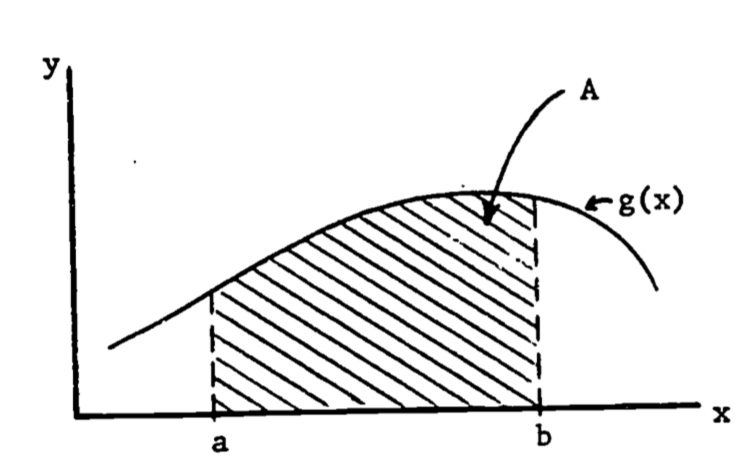
\includegraphics[width=0.75\linewidth]{figures/fig-calcint-1} \caption{Area under the curve g(x).}\label{fig:fig-calcint-1}
\end{figure}

This use of the definite integral has strong intuitive appeal. Consider the case where \(g(x) = 1\) as in figure \ref{fig:fig-calcint-2}.

\begin{figure}
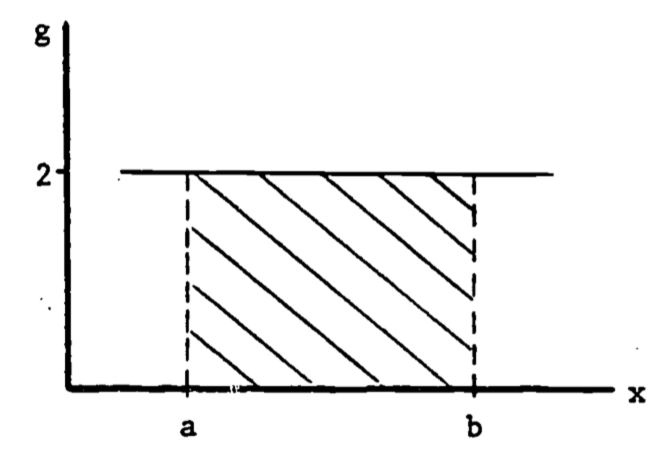
\includegraphics[width=0.75\linewidth]{figures/fig-calcint-2} \caption{Area of Rectangle.}\label{fig:fig-calcint-2}
\end{figure}

The area under \(g(x)\) is then

\[A = \int^b_a g(x)dx = \int^b_a 2 dx = 2 \int^b_a dx = 2(b-a)\]

Thus \(\int^b_a dx\) represents the width and \(g(x)\) is the height. Thus the definite a integral as area has intuitive meaning: area = height \(\times\) width. In general, the same visual identification applies:

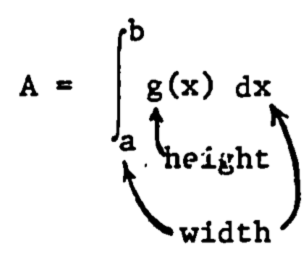
\includegraphics[width=0.25\linewidth]{figures/fig-calcint-p5}

\textbf{Example 1}

Diffusion of a gas across a membrane is often described by Fick's Law which states that the rate of transport is proportional to the product of the surface area of the membrane and the concentration gradient. Thus knowledge of the surface area is important. Certain leaves have nearly parabolic edges (fig.~\ref{fig:fig-calcint-3}). The area of the top surface available for transport of water is then found by integrating the parabola function. If the dimensions of the leaf are length = 2a, width = 2b, then the parabola describing one edge is written

\[y(x) = -bx^2/a^2 + b\]

\begin{figure}
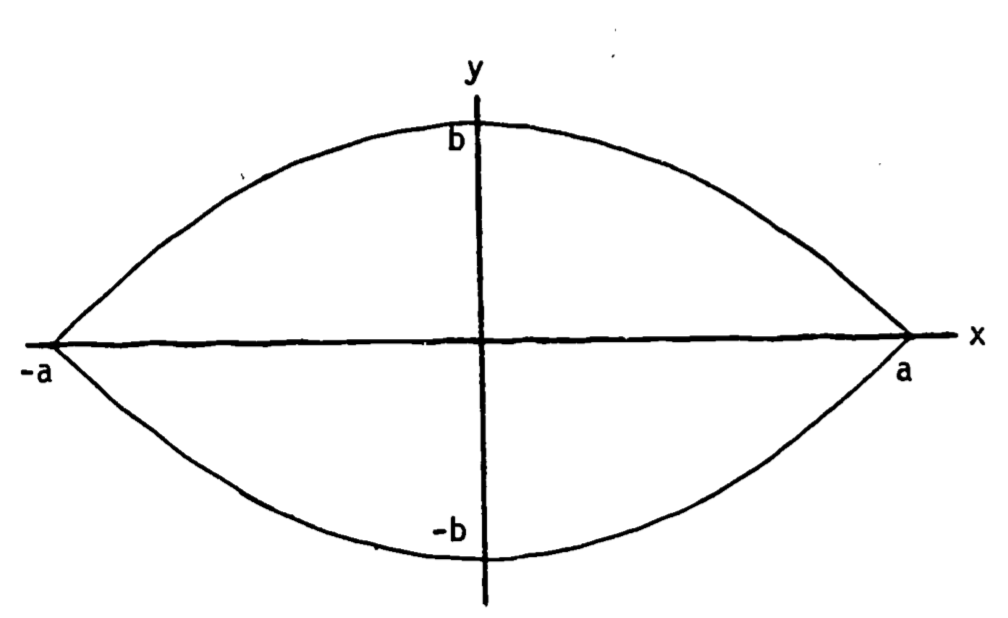
\includegraphics[width=0.75\linewidth]{figures/fig-calcint-3} \caption{Leaf with parabolic edge contours.}\label{fig:fig-calcint-3}
\end{figure}

The area of half the leaf is

\[ \frac{A}{2} = \int^a_{-a} (-bx^2/a^2 + b)dx \]

i.e., the area between the x-axis and the upper curve. Thus we calculate

\begin{align*}
A &= 2 \int^a_{-a} (-bx^2/a^2 + b)dx \\
  &= 2[-(b/a^2)x^3/3+bx]^a_{-a} \\
  &= 2[(-ab/3 + ab ) - (ab/3 - ab)] \\
  &= 8ab/3 \\
\end{align*}

\hypertarget{improper-integrals}{%
\subsection{Improper Integrals}\label{improper-integrals}}

Occasionally we are interested in long term behavior of a measured quantity. For example, when raw sewage and other chemical pollutants are continually dumped into a lake, one effect is the rapid increase in the number of microorganisms. The resultant high level of organic oxidation from metabolism of the sewage can lead to extreme oxygen depletion of the lake, with obvious detrimental effects on other aquatic life (Dugan 1972). If we know something about the rate of oxygen consumption by the microorganisms, then we obtain the amount of oxygen consumed during a time period \(T\) by integrating the rate over that time period, i.e., using, a definite integral with limits 0, \(T\). We then estimate the maximum oxygen depletion by integrating over an infinite time interval. Such a definite integral with at least one infinite limit is called an \textbf{improper integral}.

\textbf{Example 2}

Assume that self-inhibition by the microorganism population causes the oxygen depletion to taper off as time becomes large. One model might be

\begin{equation}
\frac{dC}{dt} = te^{-t^2} + e^{-t}
\label{eq:calcint-4}
\end{equation}

where \(C\) represents the quantity of oxygen consumed. A graph of \(dC/dt\) looks like figure \ref{fig:fig-calcint-4}.

\begin{figure}
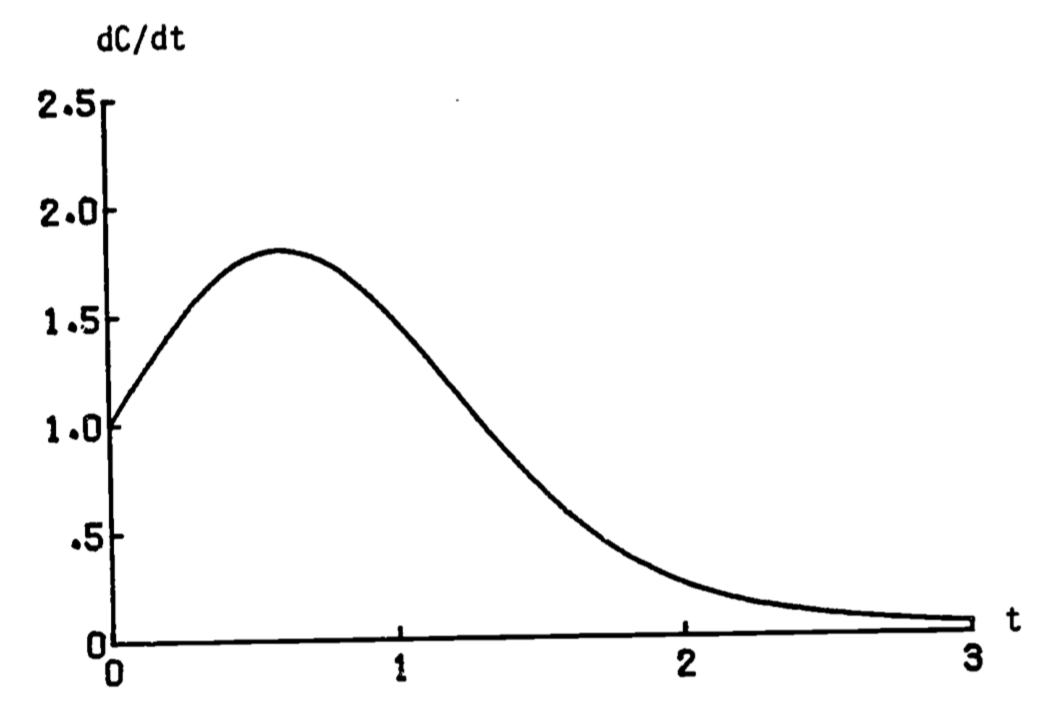
\includegraphics[width=0.75\linewidth]{figures/fig-calcint-4} \caption{Rate of oxygen consumption.}\label{fig:fig-calcint-4}
\end{figure}

The total amount of oxygen consumed by time \(T\) is then found by integrating eqn. \eqref{eq:calcint-4}.

\[C(T) = \int^T_0 (te^{-t^2} + e^{-t}) dt \]

The maximum depletion is then found by letting \(T\) increase to \(\infty\).

\[C(\infty) = \lim_{T \rightarrow \infty} \int^T_0 (te^{-t^2} + e^{-t}) dt \]
With most nicely behaved models, we can evaluate \(C(\infty)\) directly. The above integral is then written

\begin{equation}
C(\infty) = \int^\infty_0 (te^{-t^2} + e^{-t}) dt
\label{eq:calcint-5}
\end{equation}

and is evaluated as with previous definite integrals.

Some functions are not ``nicely behaved'' and certain integrals cannot be evaluated directly. If we desired to evaluate the circumference \(C\) of a tube with circular cross-section by using.an integral (instead of the well-known formula \(C = 2 \pi r\)) we can encounter difficulties. For one-quarter of the circle (fig.~\ref{fig:fig-calcint-5}) the arc-length is given by (Schwartz 1974, p.~634)

\[ L = \int^r_0 \frac{r}{\sqrt{r^2-x^2}} dx\]

where \(r\) is the radius. The integrand is infinite at \(x=r\) (fig.~\ref{fig:fig-calcint-6}). However, we can evaluate the integral by taking the limit of another integral:

\begin{align*}
L &= \lim_{a \rightarrow r} \int^q_0 \frac{r}{\sqrt{r^2-x^2}} dx \\
&= \lim_{a \rightarrow r} [r \sin^{-1} (x/r) ]^a_0 \\
&= \lim_{a \rightarrow r} [r \sin^{-1} (a/r) ] = r\pi/2 \\
\end{align*}

\begin{figure}
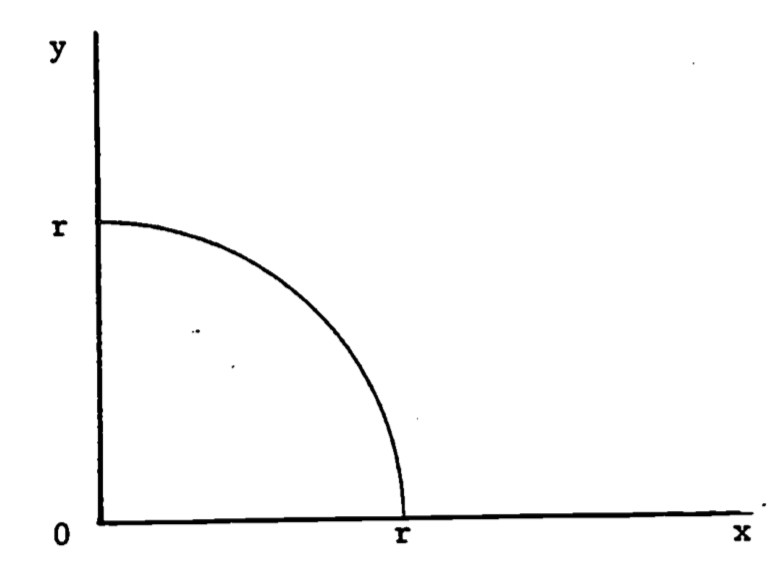
\includegraphics[width=0.75\linewidth]{figures/fig-calcint-5} \caption{The quarter-circle, $y=\sqrt{r^2 -x^2}$}\label{fig:fig-calcint-5}
\end{figure}

\begin{figure}
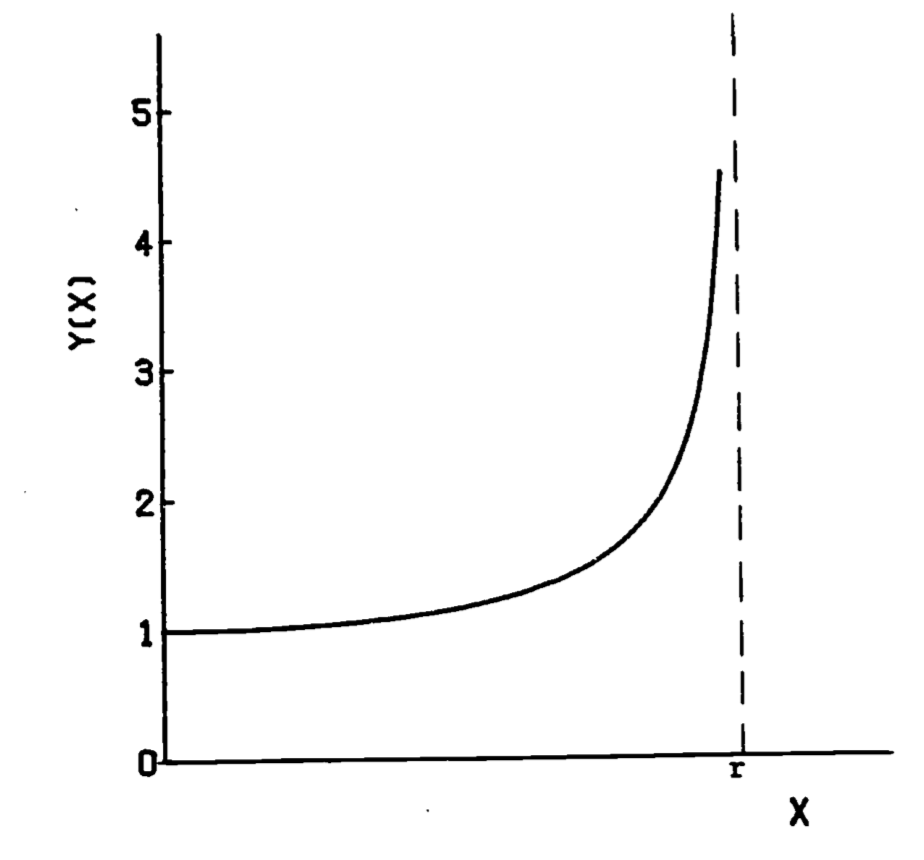
\includegraphics[width=0.75\linewidth]{figures/fig-calcint-6} \caption{Integrand of arc-length formula, $y=r/ \sqrt{(r^2 -x^2)}$}\label{fig:fig-calcint-6}
\end{figure}

\begin{center}\rule{0.5\linewidth}{0.5pt}\end{center}

\hypertarget{methods-of-integration}{%
\section{METHODS OF INTEGRATION}\label{methods-of-integration}}

Since there are no foolproof formulae that can be used for all integrals (as there are for derivatives), the following integration methods all attempt to change a difficult integral into a simpler one. All examples use definite integrals.

\hypertarget{substitution}{%
\subsection{Substitution}\label{substitution}}

This method substitutes each part of a definite integral with a counterpart so that the result is kept the same. With the substitution \(u = h(x)\), the integral

\[\int^b_a f(x)dx\]

becomes transformed into

\[\int^{h(b)}_{h(a)}g(u)du\]
where \(g(u)du = f(x)dx\). Thus the integrand, \(dx\), and the limits have been transformed into equivalent counterparts. We obtain \(g(u)\) by finding the inverse function \(h^{-1} (u)\) so that

\begin{align*}
x &= h^{-1}(u) \\
dx &= \frac{d[h^{-1}(u)]}{du} du \\
g(u)du &= [f(x)][dx] \\
g(u) &= [f(h^{-1}(u))][\frac{dh^{-1}(u)}{du}] \\
\end{align*}

Often, \(h(x)\) appears explicitly in the integrand so that \(u\) is substituted directly.

\textbf{Example 3}

The problem presented above on the oxygen depletion due to sewage dumping can now be solved. The integral in eqn. \eqref{eq:calcint-5} is first separated.

\begin{equation}
\int^{\infty}_0(te^{-t^2} +e^{-t}) dt = \int^{\infty}_0 te^{-t^2}dt + \int^{\infty}_0|e^{-t}dt
\label{eq:calcint-6}
\end{equation}

The antiderivative of \(te^{-t^2}\) is not obvious, so we substitute a new function into the integral. Let \(u = t^2\). Then the differential \(du\) is

\[du = (du/dt)dt = 2tdt\]
so that
\[\frac{du}{2} = tdt\]
The limits remain, since \(u = 0\) when \(t = 0\) and \(u = \infty\) when \(t = \infty\). Direct substitution then gives

\begin{align*}
\int^{\infty}_0 te^{-t^2}dt &= \int^{\infty}_0e^{-t^2}(tdt) \\
&= \int^{\infty}_0 e^{-u} (\frac{du}{2}) = \frac{1}{2} \int^{\infty}_0 e^{-u}du \\
&= \frac{1}{2} [-e^{-u}]^{\infty}_0 = \frac{1}{2}[0-(-1)] \\
&= \frac{1}{2} \\
\end{align*}

Since the second term in eqn. \eqref{eq:calcint-6} is now obvious \(\int^{\infty}_0 e^{-u}du = \int^{\infty}_0 e^{-t}dt=1\), we obtain the solution to eqn. \eqref{eq:calcint-5} of
\[C(\infty) = 1/2 + 1 = 3/2\]

\hypertarget{integration-by-parts}{%
\subsection{Integration by Parts}\label{integration-by-parts}}

This method utilizes a relation from differential calculus concerning the total differential. Recall that the differential of a product of two functions \(u(x)\), \(v(x)\) can be written
\[d(uv) = udv + vdu\]
If we evaluate antiderivatives, we obtain

\begin{equation}
uv = \int udv + \int vdu
\label{eq:calcint-7}
\end{equation}

Rearrangement of eqn. \eqref{eq:calcint-7} gives the integration by parts formula
\[\int udv = uv - \int vdu\]
With definite integrals, we usually write this formula as

\begin{equation}
\int^b_a [u(x)\frac{dv}{dx}]dx = [uv]^b_a - \int^b_a [v(x)\frac{du}{dx}]dx
\label{eq:calcint-8}
\end{equation}

Again, the goal is to change a difficult integral, the left side of eqn. \eqref{eq:calcint-8}, into a simpler one, the right side of eqn. \eqref{eq:calcint-8}. An example is presented later.

\hypertarget{partial-fractions}{%
\subsection{Partial Fractions}\label{partial-fractions}}

When the integrand is a ratio of two polynomials, it often can be decomposed into a sum of simpler terms. Only the case of non-repeated linear terms in the denominator is treated here. For more complicated cases in an ecological setting, see Clow and Urquhart (1974) p.~559.

The integrand is assumed to be of the form \(F(x)/G(x)\) where \(F(x)\) and \(G(x)\) are polynomial functions and where \(G(x)\) is the product of linear factors. For example,
\[G(x) = (1 + 2x)(2 + 2x)(1+x)\]
is a polynomial composed of factors linear in \(x\). The partial fraction technique replaces the single rational expression by a sum of terms where each denomination is one of the linear factors of \(G(x)\). If we have two linear factors,
\[G(x) = A(x)B(x)\]
then a partial fractions decomposition gives
\[\frac{F(x)}{G(x)} = \frac{F(x)}{A(x)B(x)} = \frac{C_1}{A(x)} + \frac{C_2}{B(x)}\]
where \(C_1\) and \(C_2\) are constants. Multiplication by \(A(x)B(x)\) gives

\begin{equation}
F(x) = C_1B(x) + C_2A(x)
\label{eq:calcint-9}
\end{equation}

Let \(r_1, r_2\) be zeros of \(A(x), B(x)\), respectively, i.e.~\(A(r_1 ) = B(r_2 ) = 0\). Then, with \(x = r_1\), eqn. \eqref{eq:calcint-9} is
\[F(r_1) = C_1 B(r_1)\]

and with \(x = r_2\), eqn. \eqref{eq:calcint-9} becomes
\[F(r_2) = C_2 A(r_2)\]
so that \(C_1,C_2\) can be easily determined.

\textbf{Example 4}

The logistic growth model for animal populations is represented as a differential equation
\[\frac{dN}{dt} = rN(1 - N/K), \;\;\;\text{where }\; r,K = \mbox{constant}\]

Separating variables (see the section, Differential Equations) gives, using the differentials \(dN\) and \(dt\),
\[\frac{dN}{N(1 - N/K)} = rdt\]
which is integrated to yield the equation

\begin{equation}
\int \frac{dN}{N(1 - N/K)} = \int rdt
\label{eq:calcint-10}
\end{equation}

The right side of eqn. \eqref{eq:calcint-10} is easily integrated. The left side, however, must be reworked. First rewrite the integral as
\[\frac{1}{N(1 - N/K)} = \frac{K}{N(K-N)}\]

Now expand in partial fractions as
\[\frac{K}{N(K-N)} = \frac{a_1}{N} + \frac{a_2}{K-N}\]
Multiplying both sides by \(N(K - N)\) gives

\begin{equation}
K = a_1(K - N) + a_2N
\label{eq:calcint-11}
\end{equation}

Since \eqref{eq:calcint-11} must hold for all values of \(N\) (Clow and Urquhart 1974, p.~562), then setting \(N = 0\) gives
\[a_1 = 1\]
and \(N = K\) gives

\[a_2 = 1\]
so that\\
\[\frac{K}{N(K-N)} = \frac{1}{N} + \frac{1}{K-N}\]
Then eqn. \eqref{eq:calcint-10} is
\[\int \frac{dN}{N} + \int \frac{dN}{K-N} = \int rdt\]
which integrates to

\[ln N - ln (K-N) = rt + C\]

\begin{center}\rule{0.5\linewidth}{0.5pt}\end{center}

\hypertarget{applications-of-definite-integrals}{%
\section{APPLICATIONS OF DEFINITE INTEGRALS}\label{applications-of-definite-integrals}}

Direct applications of integrals generally fall into discrete categories in contrast to applications of derivatives which usually are based on slopes. The first group discussed below uses the integral as the accumulation of changes in the function. The second category uses the integral as an area or generalized volume. The last application is more mathematical, although it actually relies on the accumulation concept, and uses the integral to estimate the error in a given approximation.

\hypertarget{accumulation-of-changes-in-the-function}{%
\subsection{Accumulation of Changes in the Function}\label{accumulation-of-changes-in-the-function}}

The integral as a total accumulation has been presented before in example 2 on oxygen depletion. This use of the integral is actually fairly intuitive. Let us call our quantity of interest \(F(x)\). Then \(F'(x) = dF/dx\) is certainly the rate of change of \(F(x)\) and \(F(x)\) is certainly the antiderivative of \(F'(x)\). Then integrating the \textbf{rate} of change of \(F\) gives the \textbf{total} change in \(F\).

\[\int^b_a F'(x)dx = F(x)]^b_a =  F(b) - F(a)\]
Thus the definite integral

\[\int^b_a F'(x)dx\]
is the total change in \(F(x)\) as \(x\) changes from \(a\) to \(b\).

\hypertarget{average-change}{%
\subsection{Average Change}\label{average-change}}

The average change in \(F(x)\) is then found by dividing by the change in \(x\), since the average is the change in \(F\) \textbf{per unit change} in \(x\). Note that this formula can be shown graphically as the average height of the function. For a given curve, the area under the curve equals the average height multiplied by the width. Thus the average height \(\overline y\) of a curve \(y = f(x)\) is the area \(A\) divided by the width.
\[A = \int^b_a f(x)dx = (b-a)\overline y\]
\[\overline y = \frac{A}{b-a} = \frac{1}{b-a} \int^b_a f(x)dx\]

\textbf{Example 5}

An interesting example is a study (Fisher 1963 in Warren 1971, pp.~161-163) of the effects of dissolved oxygen content and food ration on the growth rate of Coho salmon. The data appear in figure \ref{fig:fig-calcint-7}. The upper curve is well approximated by

\begin{equation}
y = 7.3 (x + 3.5) e^{-0.05x}
\label{eq:calcint-12}
\end{equation}

The lower curve is the straight line
\[y = 28\]
here \(y\) = growth rate, \(x\) = dissolved oxygen. A simple comparison of the effect of diet (restricted vs.~unrestricted ration) on growth rate is to compare the average growth rates (\(\overline y\)) for the two diets. Since the lower curve has a constant growth rate, we must have \(\overline y = 28\).

\begin{figure}
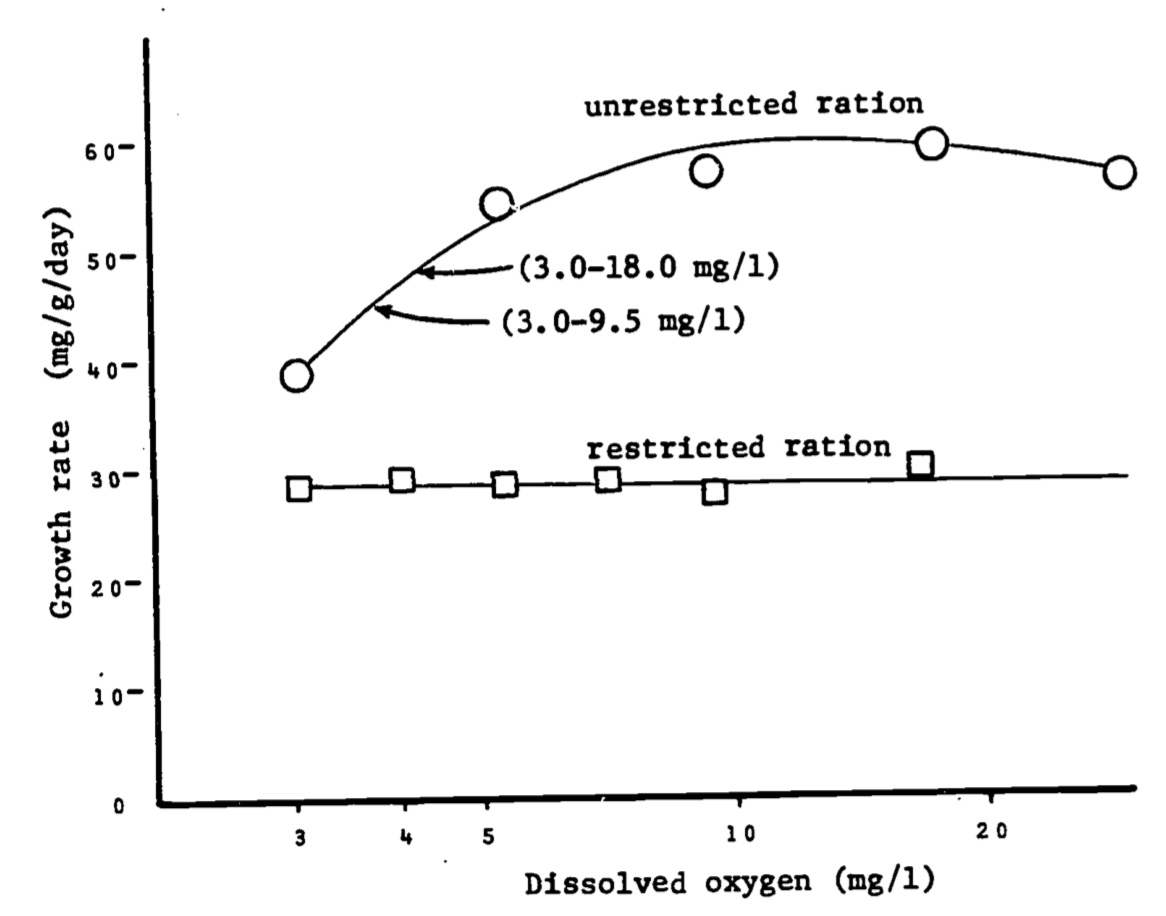
\includegraphics[width=0.75\linewidth]{figures/fig-calcint-7} \caption{Relationships between dissolved oxygen concentration and growth rate of juvenile coho salmon when food was unlimited and when it was limited. Arrows indicate growth of fish when held at oxygen concentrations fluctuating diurnally between levels specified. Data of Fisher (1963), in Warren, 1971, p. 162.}\label{fig:fig-calcint-7}
\end{figure}

\begin{align*}
\overline y = \frac{1}{27} \int^{30}_3 28dx &= \frac{1}{27}[28x]^{30}_3 = \frac{1}{27}[(28)(30)-(28(3))] \\
&= \frac{1}{27}(28)(27)=28 \\
\end{align*}

For the upper curve,
\begin{align*}
\overline y &= \frac{1}{27} \int^{30}_3 7.3(x + 3.5)e^{-0.5x}dx \\
&= \frac{7.3}{27} \int^{30}_3 3.5e^{-0.5x}dx + {\frac{7.3}{27}}\int^{30}_3 xe^{-0.05x}dx \\
&= 0.95 \int^{30}_3 e^{-0.5x}dx + 0.27\int^{30}_3 xe^{-0.05x}dx \\
\end{align*}

The first integral is the same form as in previous examples.
\[0.95 \int^{30}_3 3.5e^{-0.5x}dx = 0.95[-\frac{1}{0.05} e^{-.05x}]^{30}_3\]
\[= 19(-e^{-0.05(30)}+e^{-0.05(3)}) =12.07\]

Rather than finding the second integral in tables, we will evaluate it using \textbf{integration by parts}.

With \(dv(x)\) representing the differential of \(v(x)\), the second integral can be written
\[\int^{30}_3 xe^{-0.05x}dx = \int^{30}_3 u(x)dv(x)\]
where \(u(x) = x, dv(x) = e^{-0.05x}dx\).

Recall that integration by parts uses the formula
\[\int udv = uv - \int vdu\]
Since \(du = dx\), and \(v = \int dv = -e^{-0.05x}/0.05\), we get

\begin{align*}
\int^{30}_3 xe^{-0.05x}dx &= [{\frac{-xe^{-0.05x}}{0.05}}]^{30}_3 - \int^{30}_3 \frac{-e^{-0.05x}}{0.05}dx \\
&= \frac{1}{0.05} \bigg([-30e^{-1.5}+3e^{-0.15}]-[{\frac {e^{-0.05x}}{0.05}}]^{30}_3\bigg) \\
&= 20[-30e^{-1.5}+3e^{-0.15} + \frac{e^{-0.15}}{0.05} - \frac{e^{-1.5}}{0.05}] \\
&= 173.04 \\
\end{align*}

Thus,
\[\overline y =  12.07 + 0.27(173.04) = 58.8\]
In summary, we have the averages:

\begin{longtable}[]{@{}cc@{}}
\toprule
\textbf{ration} & \textbf{average growth rate}\tabularnewline
\midrule
\endhead
restricted & 29.3\tabularnewline
unrestricted & 58.8\tabularnewline
\bottomrule
\end{longtable}

It is somewhat surprising that the average unrestricted ration rate is over twice that of the rate for the restricted ration. The data is deceptive visually due to the close values near \(x = 3 mg/l\) and the distorted logarithmic scale.

\hypertarget{distance}{%
\subsection{Distance}\label{distance}}

Velocity is defined as the rate of change of position. Since the distance covered is the total change in position, it must equal the integral of the velocity.

For a free-falling object, the velocity is given by \(v(t) = g \cdot t\) where \(g\) is the acceleration due to gravity and \(t\) is time elapsed. The distance \(S\) covered after \(T\) seconds is given by \(S = \frac{1}{2} gT^2\) which is merely the integral of velocity.

\begin{align*}
S &= \int^T_0 v(t)dt = \int^T_0 (gt)dt \\
&= g \int^T_0 t \, dt = g[t^2/2]^T_0 \\
&= \frac{1}{2}gT^2 \\
\end{align*}

\hypertarget{volumes}{%
\subsection{Volumes}\label{volumes}}

Volumes and areas of complicated regions are also evaluated using the definite integral. Previously, the area under a curve was bounded by three straight perpendicular lines. When the bottom is not the base axis, the integration is still simple. For a region shown in figure \ref{fig:fig-calcint-8} the area is the difference between the area under curve \(f\) and the area under curve \(g\). Thus

\begin{align*}
A &= \int^b_a f(x)dx - \int^b_a g(x)dx \\
&= \int^a_b [f(x)-g(x)]dx \\
\end{align*}

Note that \([f(x)-g(x)]\) is merely the height of the region at the point \(x\), so the height times width interpretation is still applicable.

\begin{figure}
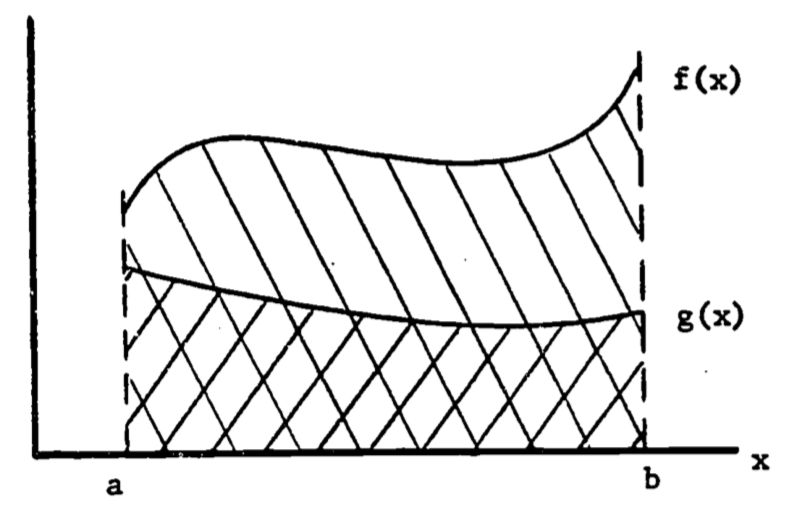
\includegraphics[width=0.75\linewidth]{figures/fig-calcint-8} \caption{Area between two curves.}\label{fig:fig-calcint-8}
\end{figure}

\hypertarget{surface-area-of-revolution}{%
\subsection{Surface Area of Revolution}\label{surface-area-of-revolution}}

When the region is not planar, the evaluation of its area must take into account the changes in the third dimension. If the surface is obtained by revolving a curve around a straight line, the evaluation needs only a single integral. The following example illustrates the method.

\textbf{Example 6}

One study of temperature regulation in mammals requires knowledge of the surface area exposed to the sun. The model views the torso of the animal as symmetric with respect to a longitudinal axis. Each vertical cross-section is then a circle. The simplest such approximation is a cylinder:

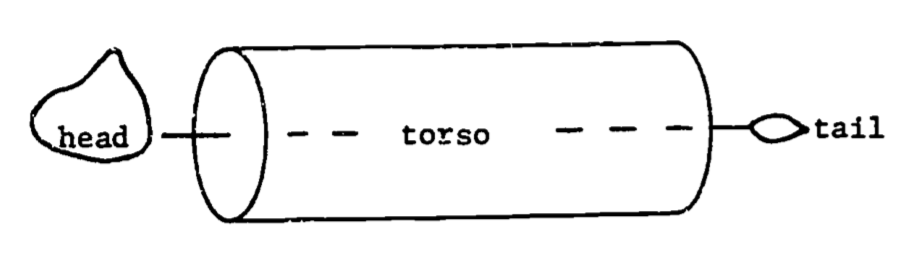
\includegraphics[width=0.5\linewidth]{figures/fig-calcint-8a}

The cylinder can be described by revolving a straight line around the axis, as in figure \ref{fig:fig-calcint-9}.

\begin{figure}
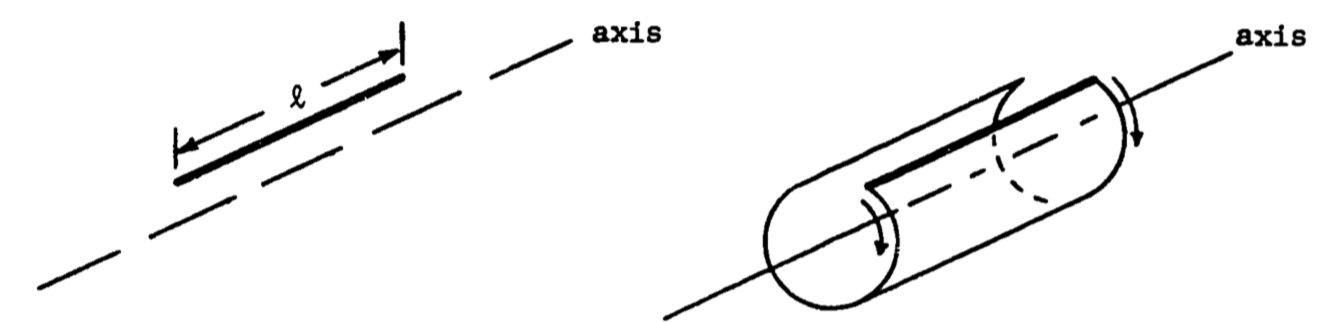
\includegraphics[width=0.75\linewidth]{figures/fig-calcint-9} \caption{Surface area of revolution: a cylinder.}\label{fig:fig-calcint-9}
\end{figure}

Unrolling the surface gives a rectangle whose width equals the circumference of the circular end face of the cylinder. This \textbf{surface area of revolution} equals the line length multiplied by the width, thus \(A=2\pi r\:l\) (fig.~\ref{fig:fig-calcint-10})

\begin{figure}
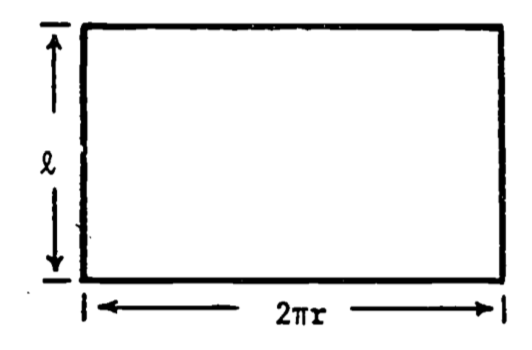
\includegraphics[width=0.25\linewidth]{figures/fig-calcint-10} \caption{Surface of unrolled cylinder.}\label{fig:fig-calcint-10}
\end{figure}

As with the area under a curve, the general formula for a surface area of revolution must be intuitive, i.e., must visually appear as length times circumference. Let the torso have a profile of varying radius:

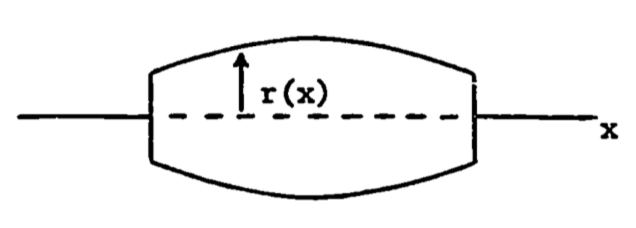
\includegraphics[width=0.5\linewidth]{figures/fig-calcint-10a}

Assume the line to be revolved is graphed as follows,

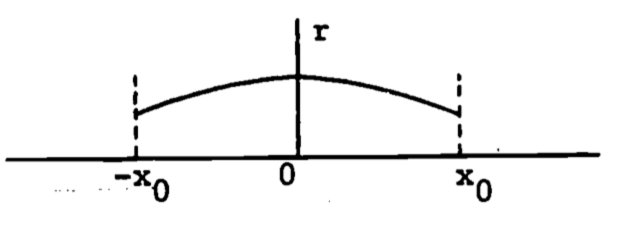
\includegraphics[width=0.5\linewidth]{figures/fig-calcint-10b}

and is represented by \(r = a - bx^2\), \(a\) and \(b\) positive constants. The radius then changes with \(x\), and the integral must be used:

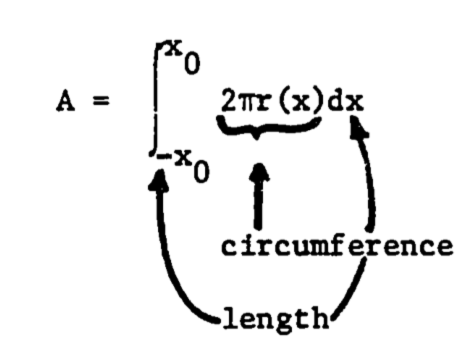
\includegraphics[width=0.25\linewidth]{figures/fig-calcint-10c}

In this example, let \(x_0 = 0.5m\), \(a = 0.28\), \(b = 0.24\). The total surface area is

\begin{align*}
A &= \int^{0.5}_{-0.5} 2 \pi(0.28-0.24x^2)dx \\
&= 2 \pi [0.28x - \frac{0.24}{3} x^3]^{0.5}_{-0.5} \\
&= 1.63 m^2 \\
\end{align*}

Note that any function will work in the formula, as long as the area desired is a surface area of revolution. The only problem might be in using a function which is difficult to integrate.

\hypertarget{volume-of-revolution}{%
\subsection{Volume of Revolution}\label{volume-of-revolution}}

The volume of a solid generated by revolving a curve around an axis can be derived as an intuitive extension of the surface area of revolution. The area and volume formulae for the cylinder and the general revolved solid (figure \ref{fig:fig-calcint-11}) are seen to be analogous.

\begin{longtable}[]{@{}lll@{}}
\toprule
& Cylinder & Revolved solid\tabularnewline
\midrule
\endhead
Surface area & \(2\pi r^2 l\) & \(\int^l_0 2\pi f(y)dy\)\tabularnewline
Volume & \(\pi r^2 l\) & \(\int^l_0 \pi[f(y)]^2 dy\)\tabularnewline
\bottomrule
\end{longtable}

\begin{figure}
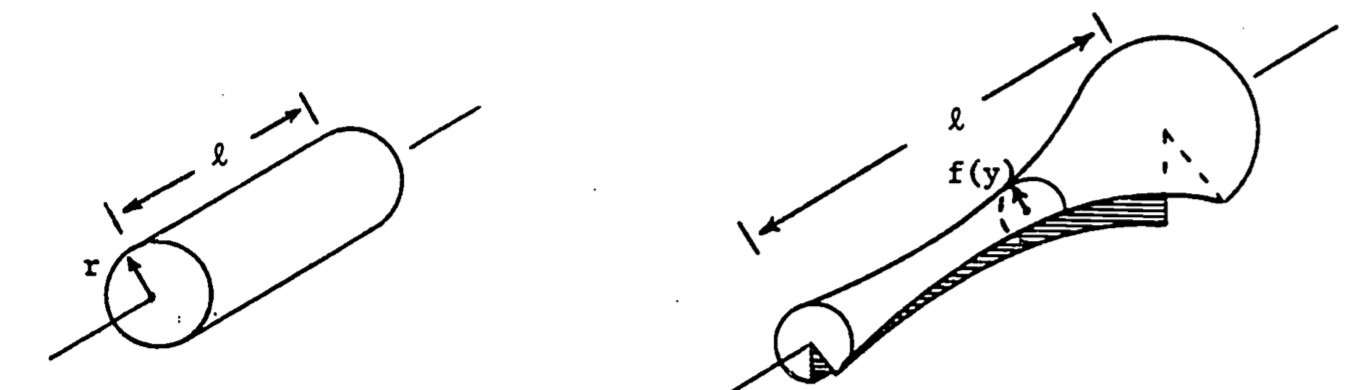
\includegraphics[width=0.75\linewidth]{figures/fig-calcint-11} \caption{Solids of revolution.}\label{fig:fig-calcint-11}
\end{figure}

Now we develop the general volume formula by expressing the integral as a limit of sums of pieces of the solid. Consider a curve \(z = f(y)\) and the region \(R\) under the curve (figure \ref{fig:fig-calcint-12}). We revolve the region \(R\) around the y-axis (figure \ref{fig:fig-calcint-13}) to obtain the solid.

\begin{figure}
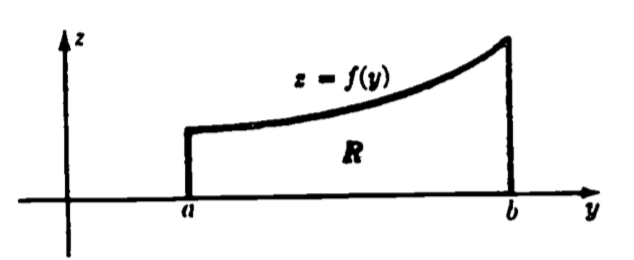
\includegraphics[width=0.5\linewidth]{figures/fig-calcint-12} \caption{The function f(y).}\label{fig:fig-calcint-12}
\end{figure}

\begin{figure}
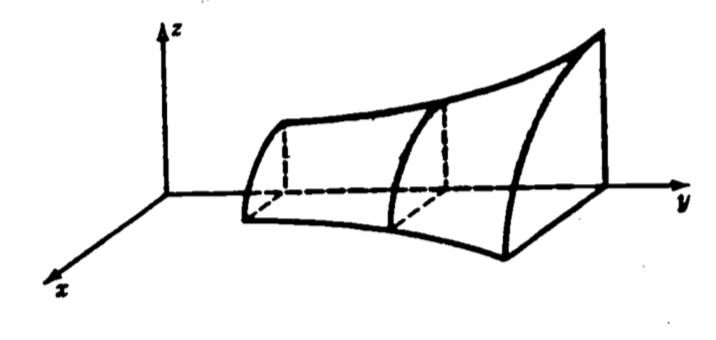
\includegraphics[width=0.5\linewidth]{figures/fig-calcint-13} \caption{The solid obtained by revolving f(y).}\label{fig:fig-calcint-13}
\end{figure}

Suppose we divide the interval \([a,b]\) into many subintervals, each of width \(dy\). Then, if \(dy\) is sufficiently small, the area of the subregion \(R_i\) is well approximated by a rectangle of width \(dy\) and height \(f(y_i)\), as figure \ref{fig:fig-calcint-14} indicates. By revolving \(R_i\) about the y-axis, we sweep out a circular slab with radius \(f(y_i)\) and thickness \(dy\) (figure \ref{fig:fig-calcint-15}).

\begin{figure}
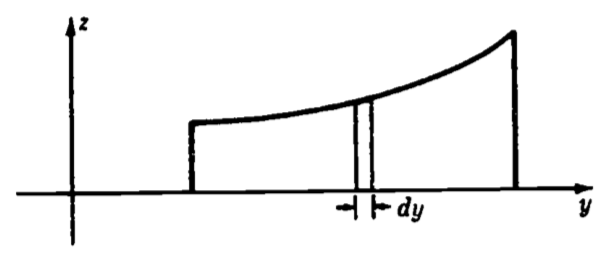
\includegraphics[width=0.5\linewidth]{figures/fig-calcint-14} \caption{The area increment dy.}\label{fig:fig-calcint-14}
\end{figure}

\begin{figure}
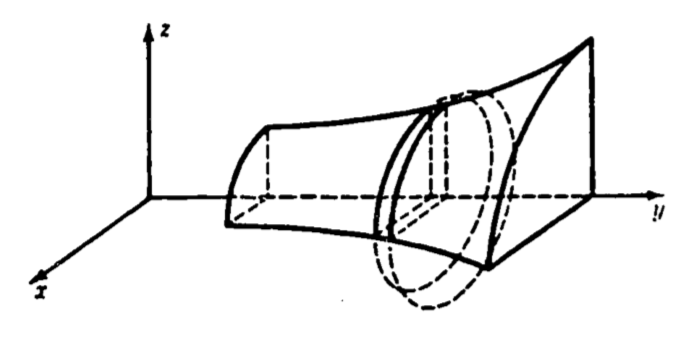
\includegraphics[width=0.5\linewidth]{figures/fig-calcint-15} \caption{The volume element obtained by revolving dy.}\label{fig:fig-calcint-15}
\end{figure}

The volume of each slab is \(\pi (radius)^2(length) = \pi f(y_i)^2dy\). Thus we have volume \(V\) of the solid as

\begin{align*}
V &= \lim_{dy \rightarrow 0} \sum^N_{i=1} \pi f(y_i)^2dy, \;\;\;\;\;\; N= (b-a)/dy \\
&= \int^b_a \pi f(y)^2 dy \\
\end{align*}

\hypertarget{general-surface-areas}{%
\subsection{General Surface Areas}\label{general-surface-areas}}

When the surface is more irregular and is not axially symmetric, its area can still be found. The surface must now, however, be described by a three dimensional function which gives the height as a function of the length and width coordinate: \(z = f(x,y)\).

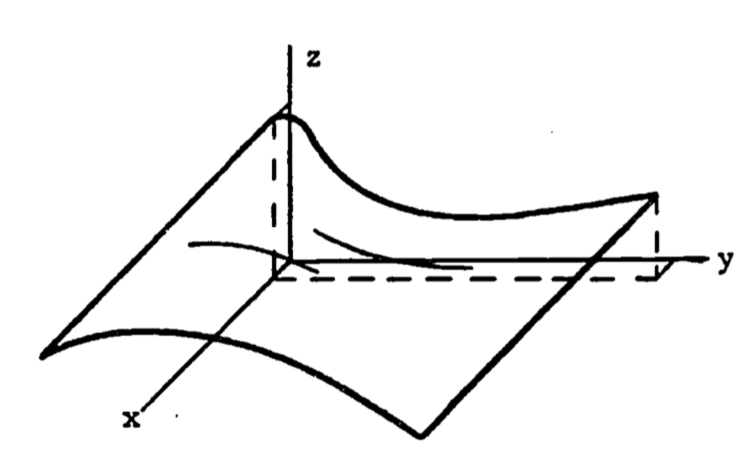
\includegraphics[width=0.5\linewidth]{figures/fig-calcint-15a}

The dependence on two variables requires two integrals, and the method used is called \textbf{double integration}.

Given a function of two variables, say \(z = f(x,y)\), we can write a \textbf{double integral} of \(z\) over a region \(R\) as:
\[F = \int_R \int f(x,y)dA \]
with \(A\) representing the area coordinates from the region \(R\). This integral is more often evaluated by writing it as an \textbf{iterated double integral}:

\[F = \int^b_a \int^{h(x)}_{g(x)} f(x,y) dy dx = \int^b_a \bigg[ \int^{h(x)}_{g(x)} f(x,y)dy \bigg] dx\]

Evaluation of the ``inner'' integral yields a function of \(x\), which becomes the integrand of the ``outer'' integral. \footnote{Note that the order of integration can be reversed when \(f(x,y)\) is continuous in \(x\) and \(y\).}

When the surface is described by \(z = f(x,y)\), its area is found using an iterated integral. The limits of integration are found by projecting the boundary of the surface onto the x,y plane. The formula for the surface area is \footnote{see Ayres (1964), p.319.}
\[A = \int^b_a \int^{h(x)}_{g(x)} [1 + (\frac{\partial z}{\partial x})^2 +(\frac{\partial z}{\partial y})^2]^{\frac{1}{2}} dy dx \]

and is best illustrated by example.

\textbf{Example 7}

If the animal is again considered to look like a cylinder, one improvement would be to account for the neck rising at an angle from the shoulder. To keep the calculations simple, we assume the neck rises vertically, and is also cylindrical (figure \ref{fig:fig-calcint-16}).

\begin{figure}
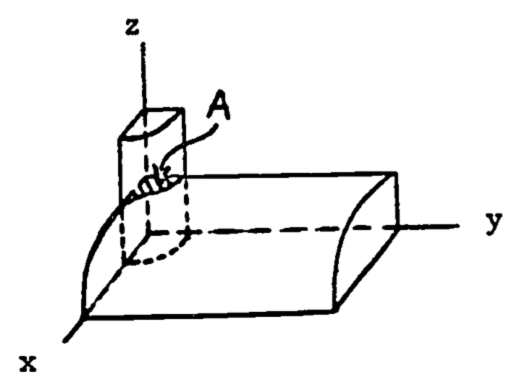
\includegraphics[width=0.75\linewidth]{figures/fig-calcint-16} \caption{Half of the upper surface.}\label{fig:fig-calcint-16}
\end{figure}

We determine the area of the torso by subtracting the ``back'' area inside the vertical cylinder, \(A\), from the area of the horizontal cylinder, which we found was \(0.25 \pi\). The equation for the ``back'' surface is \(x^2 + z^2 = (0.25)^2\). The vertical cylinder is defined by \(x^2 + y^2 = (0.10)^2\). The projection is then half a circle of radius 0.10 (figure \ref{fig:fig-calcint-17}), and is given by \(y = \sqrt {0.10^x - x^2}\).

\begin{figure}
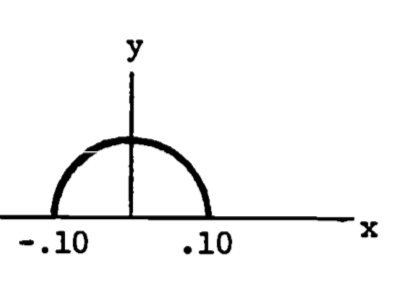
\includegraphics[width=0.5\linewidth]{figures/fig-calcint-17} \caption{Projection of the "neck" region.}\label{fig:fig-calcint-17}
\end{figure}

For a given \(x\), \(y\) varies from 0 up to \(\sqrt {0.10^x - x^2}\) . The limits on \(x\) are -0.10 to 0.10. The equation for the surface of the back yields the required partial derivatives:
\[ \frac{\partial z}{\partial x} = - \frac{x}{\sqrt{0.25^2 - x^2}},\;\;\; \frac{\partial z}{\partial y} = 0  \]
\[A = \int^{0.10}_{-0.10} \int^{\sqrt{0.10^2-x^2}}_0 [1 + \frac{x^2}{0.25^2 - x^2} + 0] dy \, dx\]
This strange formula still has visual intuitive appeal since the limits on \(y\) are obtained from the \textbf{width} in the \(y\) direction (for a given \(x\)) and the limits on \(x\) are from the \textbf{length} in the \(x\) direction. The quantity in brackets accounts for the changing height of the surface. The remaining parts of the problem are left as an exercise.

\hypertarget{error-estimation}{%
\subsection{Error Estimation}\label{error-estimation}}

The integral can be used to develop approximate solutions to certain equations or approximate models of given data. The integral provides a qualitative error estimate for the approximation. The most well known application is the least squares fit of a line through a set of data points. One of the most recent applications is the residual norm as an error indicator for approximate solutions to partial differential equations. In each example discussed below, a function is integrated over a domain of interest. If this function represents the difference between the approximate and true solution, then the value of the integral decreases as the approximation improves. The integral is then minimized to provide the ``best'' approximation.

\hypertarget{least-squares}{%
\subsubsection{Least Squares}\label{least-squares}}

Many experiments produce data as pairs of numbers
\[(x_1,y_1),(x_2,y_2), \ldots, (x_n,y_n)\]
The underlying relationship is often assumed to be linear, that is, the model is assumed to be
\[y = Ax + B, \text{ where }A,B = \text{constants}\]
The points (\(x_i,y_i\)) are usually not collinear (see figure \ref{fig:fig-calcint-18}) due to experimental error, inaccuracies in the model, round-off error during measurement, etc. Thus the problem is to choose the constants \(A,B\) so the line matches the data points as closely as possible. The method of least squares uses the sum of squared deviations for the error function, \(E^2\) (see figure \ref{fig:fig-calcint-18}):

\begin{equation}
E^2 = \sum^n_{i=1} [y(x_i)-y_i]^2
\label{eq:calcint-13}
\end{equation}

where \(y(x_i) = Ax_i + B\). The goal is then to choose \(A\), \(B\) so that \(E^2\) is minimal. By writing \(E^2\) as a function of the parameters \(A\), \(B\), we minimize \(E^2\) by setting the partial derivatives equal to zero:
\[\frac{\partial E^2}{\partial A} = 0,\;\; \frac{\partial E^2}{\partial B} = 0\]

\begin{figure}
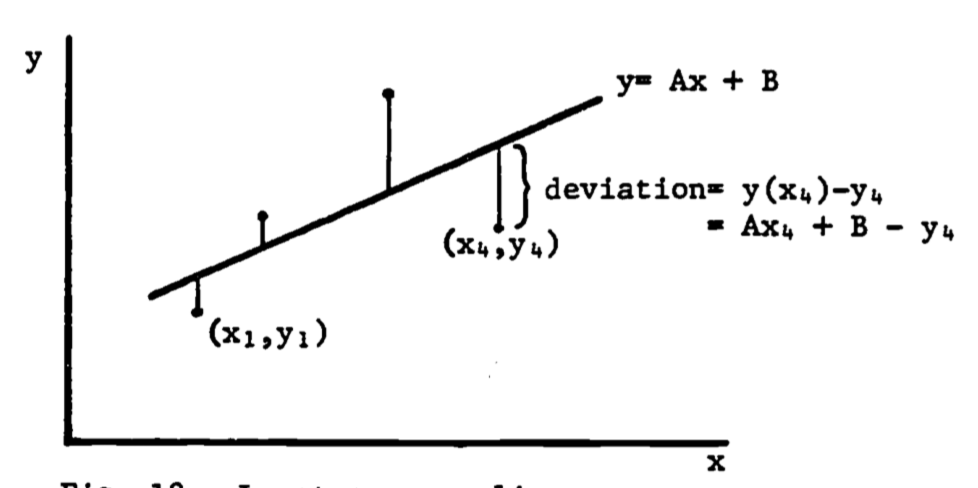
\includegraphics[width=0.75\linewidth]{figures/fig-calcint-18} \caption{Least-squares line.}\label{fig:fig-calcint-18}
\end{figure}

We then obtain two linear equations in \(A\), \(B\) which are easily solved (see problem 5) and can be shown to give the line with the least sum of squared deviations (see problem 6).

\hypertarget{norms}{%
\subsubsection{Norms}\label{norms}}

The squared deviation used in the least squares method is an example of a \textbf{norm}. A norm of a function \(f(x)\), denoted \(\|f(x)\|\), is a function (Pearson 1974, p.~946) such that, for any scalar \(\alpha\), and any functions \(f(x), g(x)\),
\[\|f(x)\| \ge 0\]
\[\|f(x)\| = 0\]
if and only if \(f(x) = 0\)
\[\| f (x) \| = |\alpha| \cdot \| f (x) \|\]
\[\| f (x) + g(x) \| \le \| f (x) \| + \|g(x) \| \]

When a curve \(y = f(x)\) is approximated by a least-squares straight line \(y = Ax + B\) over the interval \([a,b]\), we choose \(A\), \(B\) to minimize the error norm \(E\) defined by

\begin{equation}
 E^2 = \int^b_a [Ax + B - f(x)]^2 dx
\label{eq:calcint-14}
\end{equation}

Note that equation \eqref{eq:calcint-13} is a discrete analog of equation \eqref{eq:calcint-14}.

The norm can be used for evaluating the closeness of fit of one curve to another, or for obtaining a qualitative estimate of the accuracy of an approximate solution to an equation. The \(L_p\) norm of a function \(f(x)\) is defined as
\[L_p (f(x)) = \| f(x)\|_\rho = \bigg[\int^b_a |f(x)|^P dx\bigg]^{1/p}   \]

The least squares norm \(E\) is in fact \(L_2 (f(x))\), since
\[\| f(x) \|_2 = \bigg[ \int^b_a |f(x)|^2 dx\bigg]^{1/2}\]
and thus
\[E^2 = [\|f(x)\|_2]^2 = [L_2(f(x))]^2\]

\textbf{Example 8}

An interesting comparison is between the line fitted to the data points of example 5 and the line fitted to the smooth exponential curve of eqn. \eqref{eq:calcint-12}, rewritten as follows.

\begin{equation}
y_1 = 7.3 (x + 3.5) e^{-0.05x}
\label{eq:calcint-15}
\end{equation}

We can approximate this function with a linear function,

\begin{equation}
y_2 = Ax + B
\label{eq:calcint-16}
\end{equation}

by choosing \(A\) and \(B\) to minimize the \(L_2\) (least squares) norm of the difference between them, \(y_1 - y_2\). Denote the norm by
\[E = \|y_1 - y_2\|_2 = [\int^{30}_3 (y_1-y_2) dx]^{1/2}\]
Substituting eqns. \eqref{eq:calcint-15} and \eqref{eq:calcint-16} yields

\begin{equation}
E = [\int^{30}_{3} (7.3[x+3.5]e^{-0.05x} - Ax - B)^2dx]^{1/2}
\label{eq:calcint-17}
\end{equation}

We now minimize \(E\) by taking partial derivatives with respect to \(A\) and \(B\) (see Hertzberg 1977 for a review of differentiation). One first derivative will now be calculated, with the remainder of the minimization left as computer exercise 2.

First, note that the minimum of \(E\) occurs at the same values of \(A\) and \(B\) which minimize \(E_2\), since \(E\) is positive. The derivative of \(E_2\) with respect to \(A\) is now attempted. First, we write
\[\frac{\partial(E^2)}{\partial A} = \frac{\partial}{\partial A} \bigg[ \int^{30}_3 f(A,B,x)dx\bigg] \]
where
\[ f(A,B,x) = (7.3[x+3.5]e^{-0.05x}-Ax - B)^2\]
Then the derivative is calculated after the integration is completed, which is not a simple task. It may be easier to differentiate under the integral sign first, and then integrate the result.

\textbf{Theorem} (Pearson 1974, p.~100).

Let \(f(x,y)\) be an integrable function of \(x\) for each \(y\), and let \(\partial f / \partial y\) be continuous over \(a \le x \le b, c \le y \le d\). Then
\[\frac{d}{dy} \int^b_a f(x,y)dx = \int^b_a (\partial f / \partial y)dx\]

Thus we evaluate:

\begin{equation}
\frac{\partial (E^2)}{\partial A} = \int^{30}_3 \frac{\partial f}{\partial A} dx \\ 
 = \int^{30}_3 2(7.3[x+3.5]e^{-0.05x}-Ax-B)(-x)dx
\label{eq:calcint-18}
\end{equation}

which can now be integrated (computer exercise 2).

No justification has yet been given for the constants in eqn. \eqref{eq:calcint-15}. These, too, may be determined by a least squares norm. See computer exercise 1 for details.

The norm can also be used to estimate qualitatively the relative accuracies of approximate solutions to a differential equation. The limits are determined as above by the interval in which the accuracy is to be judged. An example is presented in the next section.

\begin{center}\rule{0.5\linewidth}{0.5pt}\end{center}

\hypertarget{differential-equations}{%
\section{DIFFERENTIAL EQUATIONS}\label{differential-equations}}

As was previously mentioned, the integral is also used to solve a differential equation. In the simplest form, if an equation is written as
\[\frac{dx}{dt} = f(t)\]
then the solution (general solution) is
\[x(t) = \int f(t)dt\]
If we know the value of \(x\) at \(t = 0\), the \textbf{initial condition}, then the differential equation has a unique solution given by
\[x(t) = \int^t_0 f(\tau)d \tau + x(0)\]

\hypertarget{separation-of-variables}{%
\subsection{Separation of Variables}\label{separation-of-variables}}

When the differential equation also involves \(x\) on the right-hand side, the solution is not so easily represented. Other techniques must then be employed to represent the problem by a set of integrals whose integrands are functions of only the variable of integration. One such technique is separation of variables.

\textbf{Example 9}

Let us return to example 4. The equation is

\begin{equation}
\frac{dN}{dt} = rN(1 - N/K)
\label{eq:calcint-19}
\end{equation}

The simple representation given above fails here:
\[N(t) = \int rN(1 - N/K)dt\]
To integrate, we need to know \(N\) as an explicit function of \(t\), which of course we do not know. However, by multiplying both sides of eqn. \eqref{eq:calcint-19} by the differential \(dt\), we obtain
\[dN = rN(1 - N/K)dt\]

and by dividing by \(N(1 - N/K)\) we successfully separate the variables \(N\), \(t\) on either side of the equality:
\[\frac{dN}{N(1- N/K)} = rdt\]

Integration is now possible since each integrand is a function of just the variable of integration.
\[\int \frac{1}{N(1- N/K)} dN = \int rdt\]

How are initial conditions incorporated now? Since the indefinite integral produces an integration constant, the constant is determined by the initial condition, making the general solution unique.

\textbf{Example 10}

A recent study on water purification (Dickson, et al, 1977) included the mortality of fish due to intermittent chlorination. The following data were obtained (Table A) where frequency is the number of doses per 24 hours.

\begin{quote}
Table A. Fish Mortality Due to Intermittent Chlorination
\end{quote}

\begin{longtable}[]{@{}ccc@{}}
\toprule
Mortality & Frequency & Duration (hr)\tabularnewline
\midrule
\endhead
0.01 & 1 & 1.5\tabularnewline
& 2 & 0.7\tabularnewline
& 4 & 0.3\tabularnewline
0.10 & 1 & 3.2\tabularnewline
& 2 & 1.4\tabularnewline
& 4 & 0.7\tabularnewline
0.20 & 1 & 4.3\tabularnewline
& 2 & 2.0\tabularnewline
& 4 & 0.9\tabularnewline
0.50 & 1 & 7.5\tabularnewline
& 2 & 3.4\tabularnewline
& 4 & 1.6\tabularnewline
\bottomrule
\end{longtable}

A mathematical model has been devised which shows the effect of duration (\(T\)) and frequency (\(F\)) on mortality (\(M\)) using two differential equations:

\begin{equation}
\partial M / \partial T = a_1T^{1.5}
\label{eq:calcint-20}
\end{equation}

\begin{equation}
\partial M / \partial F = a_2 F^{1.8}
\label{eq:calcint-21}
\end{equation}

where \(a_1\) is a function of \(F\) and \(a_2\) is a function of \(T\). Another model was derived by curve fitting, using Table A and is quite different. For a given \(M\),

\begin{equation}
ln(T)=b_1 - b_2 \ln F
\label{eq:calcint-22}
\end{equation}

where it is now assumed that \(b_1\) is a function of \(M\):
\[b_1 = 2.16 + 0.40 \ln M\]

Can both of these models hold? Are they consistent? We can answer this by integrating the first model to derive a single expression for \(M\) as a function of \(F, T\). Each equation \eqref{eq:calcint-20}, \eqref{eq:calcint-21} involves a single partial derivative, so that one of the variables can be assumed constant. By holding \(F\) constant, we integrate eqn. \eqref{eq:calcint-20} to obtain
\[M = (a_1/1.5)T^{2.5} + C_1\]
which is more precisely written, with \(a_1\) as a function of \(F\), as

\begin{equation}
M = \frac{a_1(F)}{1.5}T^{2.5}+C_1
\label{eq:calcint-23}
\end{equation}

Similarly, we integrate eqn. \eqref{eq:calcint-21} with respect to \(F\), holding \(T\) constant.

\begin{align*}
M &= \int a_2 F^{1.8} dF = (a_2 / 1.8) F^{2.8} + C_2 \\
&= \frac{a_2(T)}{1.8} F^{2.8} +C_2 \\
\end{align*}

Thus
\[\frac{a_1(F)}{1.5} T^{2.5} +C_1 = \frac{a_2(T)}{1.8}F^{2.8} +C_2\]

We assume no observable mortality if no chlorination occurs, so that, if \(F = 0\) or \(T = 0\), then \(M = 0\). Thus \(C_1= C_2 =0\).
\[\frac{a_1(F)}{1.5} T^{2.5} = \frac{a_2(T)}{1.8} F^{2.8}\]
Therefore, we must conclude that
\[a_1(F) = 1.5C F^{2.8}\]
\[a_2(T) = 1.8C T^{2.5}\]
where \(C\) is some proportionality constant. From eqn. \eqref{eq:calcint-23} we have

\begin{equation}
M = C F^{2.8} T^{2.5}
\label{eq:calcint-24}
\end{equation}

It is now straightforward to manipulate eqn. \eqref{eq:calcint-22} to look like eqn: \eqref{eq:calcint-24}.
\[\ln T = (2.16 + 0.40 \ln M) - b_2 \ln F\]
\[\frac{\ln T + b_2 \ln F - 2.16}{0.40} = \ln M\]
\[\frac{\ln T + ln(F^{b_2}) - \ln(e^{2.16})}{0.40} = \ln M\]
\[2.5 \ln (TF^{b_2}/8.7) = lnM\]
\[\ln[(TF^{b_2} /8.7)^{2.5} ] = \ln M\]
\[T^{2.5} F^{2.5b_2} /(8.7^{2.5} ) = M\]
Thus, \(b_2 = 2.8/2.5 = 1.1, \;\;C = 1/(8.7)^{2.5} = 0.0045\) and the models agree.

\hypertarget{residual-norm}{%
\subsection{Residual Norm}\label{residual-norm}}

Often a differential equation cannot be solved by any standard methods and an approximate solution is developed. In some cases, bounds on the error in the approximation can be derived. Too often, however, calculating the error bounds is as complicated as determining the solution itself. A recent idea is to use the least-squares norm (or occasionally some other norm) as a gauge of the accuracy of the approximation. With only the differential equation at hand, a new type of norm, the residual norm, is used.

Consider a differential equation written as
\[\frac{dx}{dt} = f(x,t)\]

with initial condition \(x(0) = x_0\). If the equation is rewritten as
\[dx/dt - f(x,t) = 0\]

then we obtain an expression which vanishes when the exact solution is used. In operator notation the equation is
\[L(x,t) = 0\]
where \(L\) is the differential operator defined by
\[L(x,t) = dx/dt - f(x,t)\]
If \(L\) operates on an approximate solution, \(\overset\sim x (t)\), then \(L(\overset\sim x) \neq 0\), and its value is the \textbf{residual}. Yet we would expect \(L(\overset\sim x)\) to be small if \(x\) is a good approximation. The final step is to decide on some interval over which the approximation's accuracy is to be judged, say \([a,b]\). Then the least-squares residual norm for the approximate solution \(\overset\sim x (t)\) is
\[\| R(\overset\sim x) \|_2 = [\int^b_a (L(\overset\sim x,t))^2 dt]^{1/2} \]

Note that \(\| R(\overset\sim x) \|_2 = 0\) if the exact solution is used, since \(L\) is then 0. This limiting behavior suggests the residual norm as a \textbf{qualitative} indicator of the accuracy of an approximate solution. No theory exists, however, for estimating the \textbf{actual} error from the value of the residual norm.

\textbf{Example 11}

A deer population is threatened by severe storms as well as reduced grazing area due to a small fire. Consequently, a moratorium on deer hunting is imposed until the deer population returns to 60\% of the carrying capacity for the area. How long should the moratorium be imposed?

Assumptions are now presented which allow us to model the population dynamics of the deer and estimate the duration of the moratorium. Let the logistic growth model be used:
\[\frac{dn}{dt} = Rn(1-n/K)\]

Assume that the current population size is 400, the carrying capacity (\(K\)) is 2000, the intrinsic growth rate (\(R\)) is 1.0 and that the approximate solutions should be fairly accurate for the first three years. Assume also that the moratorium is not obeyed immediately, so that hunting pressure gradually tapers off. Let the growth model with the ``harvesting'' (i.e.~hunting) term be

\begin{equation}
\frac{dn}{dt} = Rn(1-n/K) - e^{-t}n
\label{eq:calcint-25}
\end{equation}

with initial condition \(n(0)-n_0\).

Assume also that you do not have access to either a programmable calculator or a computer. This equation cannot be solved by separation of variables (try it), so some approximation must be made. From previous studies, you learn that the following two models have been used fairly successfully to model short term population growth.

\begin{equation}
n_1(t) = (K-n_0)(1-e^{-Rt/5} ) + n_0
\label{eq:calcint-26}
\end{equation}

\begin{equation}
n_2(t) = n_0 e^{Rt/3}
\label{eq:calcint-27}
\end{equation}

Note that \(n_1(t)\) tapers off at the carrying capacity, but \(n_2(t)\) is exponential growth for \(n_2 \approx 0\); both are properties the exact solution must possess. Which approximation is better? We compare \(n_1\) and \(n_2\) by evaluating their least-squares residual norms. Rewrite eqn.\eqref{eq:calcint-25} as \(L(n) = 0\), where \(L(n)\) represents the differential operator acting on \(n\):
\[L(n) = dn/dt - Rn(1-n/K) + e^{-t}n = 0 \]

We expect a good approximate solution, \(n_a\), to give
\[L(n_a) \approx 0\]
and thus its residual norm should also be small:
\[ \| R(n_a) \|_2 \equiv [\int^T_0 (L(n_a))^2 dt]^{1/2} \approx 0\]
Intuitively, the smaller \(\| R \|_2\) is, the better the approximation should be. For this example, assume the following values:
\[K = 2000, \; R=1, \; n_0=400, \; T=3\]

The integrands in \(\| R(n_1) \|_2\) and \(\| R(n_2) \|_2\) are now calculated. From eqn. \eqref{eq:calcint-26} we obtain, after a few steps,

\begin{equation}
[L(n_1)]^2 = (2000 e^{-t}- 1600 e^{-1.2t} + 1280 e^{-0.4t} -2800 e^{-0.2t} +1600)^2
\label{eq:calcint-28}
\end{equation}

From eqn. \eqref{eq:calcint-27} we obtain

\begin{equation}
[L(n_2)]^2=[ (400/3) e^{t/3} - (1-400 e^{t/3}/2000 -e^{-t}) 400 e^{t/3}]2
\label{eq:calcint-29}
\end{equation}

After multiplying out the square in each equation and collecting terms, we can write both \eqref{eq:calcint-28} and \eqref{eq:calcint-29} as sums of exponential functions, and thus both can be integrated by hand easily (but tediously). The results are, upon integrating over the interval \([0,3]\):
\[\| R(n_1) \|_2 = 661.8\]
\[\| R(n_2) \|_2 = 172.3\]
Figure \ref{fig:fig-calcint-19} shows the accuracy of the two approximate solutions as compared to a numerical solution to the original differential equation \eqref{eq:calcint-25}. It appears that, for the chosen values of \(R\), \(K\) and \(n_0\), the approximation \(n_2(t)\) is better, and the residual norm for \(n_2\) supports this evaluation. The 60\% of carrying capacity, i.e.~1200, is reached in 3.30 years using \(n_2(t)\), and in 3.08 years according to the numerical solution \(n(t)\). It is interesting that, without the term for hunting (curve \(n_0(t)\) in fig.~\ref{fig:fig-calcint-19}), the population reaches the 60\% level in only 1.79 years.

\begin{figure}
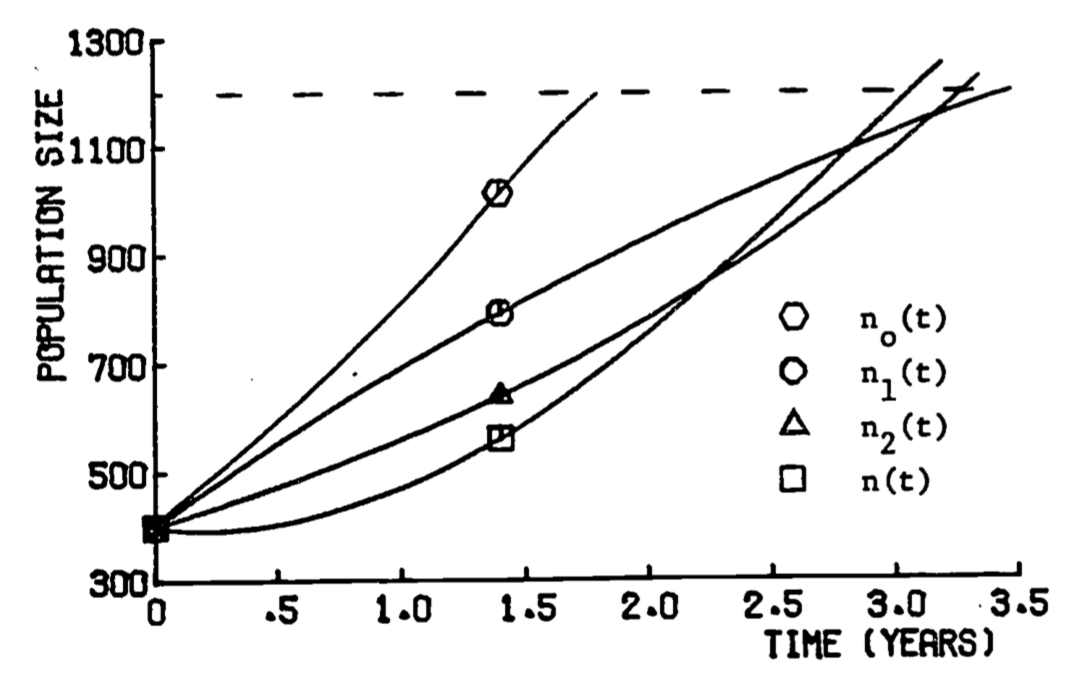
\includegraphics[width=0.75\linewidth]{figures/fig-calcint-19} \caption{Approximate growth functions}\label{fig:fig-calcint-19}
\end{figure}

\begin{center}\rule{0.5\linewidth}{0.5pt}\end{center}

\hypertarget{references-and-recommended-texts}{%
\section{REFERENCES AND RECOMMENDED TEXTS}\label{references-and-recommended-texts}}

\textbf{Calculus}

Allen, R. C.,Jr.~and Wing, G. M. 1973. Problems for a computer-oriented course. Prentice-Hall, Englewood Cliffs, N. J., 206 pp.

Ayres, F., Jr.~1964. Theory and problems of differential and integralsecond ed., Schaum's Outline Series, McGraw-Hill, New York

Baxter, W. E. and Sloyer, C. W. 1973. Calculus with probability for the life management sciences, Addison-Wesley, Reading, Ma. 648 pp.

Bittinger, M. L. 1976. Calculus: A modeling approach, Addison-Wesley,Reading, Ma.

Clow, D. J. and Urquhart, N. S. 1974. Mathematics in biology, Norton, NewYork, 727 pp.

Coughlin, R. F. 1976. Applied, calculus, Allyn and Bacon, Boston, Ma.

Hertzberg, R. C. 1979. Calculus-differentiation. An instructional module: Physical processes in terrestrial and aquatic ecosystems. Ctr. Quantitative Sci., Univ. Washington, Seattle, 64 pp.

Keisler, H. J. 1971. Elementary calculus: An approach using infinitesimals, Prindle, Weber and Schmidt, Boston, Ma.

Schwartz, A. 1974. Calculus and analytical geometry. Third ed., Holt, Rinehart and Winston, New York, 1140 pp.

Sternberg, W., Walker, R. J. et al.~1968. Calculus, a computer oriented presentation, The Center for Research in College Instruction in Science and Mathematics (CRICISAM), Florida State University, Tallahassee.

\textbf{General}

Dickson, K., Cairns, J., Jr., et al.~1977. Effects of intermittent chlorination on aquatic organisms and communities. J. Water Poll. Control Fed., 49, 35-44.

Dugan, P. R. 1972. Biochemical ecology of water pollution. Plenum Press, New York, 159 pp.

Gales, L. 1979. User's guide for subroutine PRNT3D. An instructional module: Physical processes in terrestrial and aquatic ecosystems. Ctr. Quantitative Sci., Univ. Washington, Seattle, 27 pp.

Gold, H. 1977. Mathematicalmodelingof biological systems. Wiley-Interscience,New York, 357 pp.

Handbook of applied mathematics. 1974. C. Pearson, ed.~Van NostrandReinhold, New York, 1265 pp.

Warren, C. E. 1971. Biology and water pollution control. W. B. Saunders, Philadelphia, 434 pp.

\textbf{Tables}

Handbook of Mathematical Functions, 1964. Abramowitz, M. and Stegun, I., eds., National Bureau of Standards, Applied Mathematics Series, 55, Washington, D.C.

Handbook of Mathematical Tables, 1964. Weast, R. C., Selby, M. and Hodgman, C. D., eds., The Chemical Rubber Co., Cleveland.

\begin{center}\rule{0.5\linewidth}{0.5pt}\end{center}

\hypertarget{problem-set}{%
\section{PROBLEM SET}\label{problem-set}}

\textbf{General}

\begin{enumerate}
\def\labelenumi{\arabic{enumi}.}
\tightlist
\item
  An application of both the definite integral and exponential growth is modelling demand for natural resources. Assume \(P(t)\) represents the rate of use of a resource at time \(t\geq0\), and \(P(t)\) represents the rate of consumption at time \(t = 0\). The exponential model then gives \(P(t) = P_0 e^{kt}\). The constant \(k\) can be defined as the rate of increase in the use of this resource. Let \(A(T)\) represent the amount of resource used during the interval \([0,T]\), \(T\geq0\).
\end{enumerate}

\begin{enumerate}
\def\labelenumi{\alph{enumi}.}
\tightlist
\item
  Write the definite integral representing \(A(T)\) in terms of a general function \(P(t)\).
\item
  Evaluate the integral for general \(T\geq0\) by substituting the above exponential function for \(P(t)\).
\item
  In 1973 (say \(t = 0\)), the world use of copper was estimated to be 6.99 x 10\textsuperscript{9} kg, and the demand was increasing at an exponential rate of 8\% per year. How many tons of copper will then be used from 1973 to 1983? (Hint: First find \(P_0\), \(k\), \(T\) and then use your answer to b.)
\item
  If the rate of growth in demand for copper remains at 8\% and no new reserves are discovered, when will the world supply of copper be exhausted? Assume the reserves in 1973 are 336 x 10\textsuperscript{9} kg, and no recycling occurs.
\end{enumerate}

\begin{enumerate}
\def\labelenumi{\arabic{enumi}.}
\setcounter{enumi}{1}
\tightlist
\item
  Five thousand trout, each weighing 80 grams, are planted in a lake. The population size, \(N(t)\), declines exponentially according to the equation \(N(t) = 5000e^{-0.5t}\) where \(t\) is measured in months. Each fish grows according to the formula \(W(t) = 10000 (1 - 0.8e^{-0.05t})^3\) where \(W\) is the weight in grams.
\end{enumerate}

\begin{enumerate}
\def\labelenumi{\alph{enumi}.}
\tightlist
\item
  Check that both \(N(t)\) and \(W(t)\) satisfy the given initial conditions.
\item
  Write the formula for the biomass (total weight of all the planted trout) in the lake as a function of \(t\), and calculate the biomass at 12 months.
\item
  What is the average biomass for the first 12 months? What was the initial biomass? Sketch how you think the graph of biomass versus time would appear. Mark on the vertical axis the initial, final and average biomass values.
\end{enumerate}

\begin{enumerate}
\def\labelenumi{\arabic{enumi}.}
\setcounter{enumi}{2}
\tightlist
\item
  Assume that a radioactive element disintegrates so that the number (\(N\)) of atoms present at a given time (\(t\)) decreases at a rate proportional to \(N\) itself. Let \(k\) be the constant of proportionality and \(N_0\) be the number of atoms present at \(t = 0\) (thus \(N(0) = N_0\)).
\end{enumerate}

\begin{enumerate}
\def\labelenumi{\alph{enumi}.}
\tightlist
\item
  With the derivative representing the rate of change of \(N\), use the above defined parameters and variables to write an equation for the rate of decrease in the number of radioactive atoms with passing time.
\item
  Solve this differential equation for \(N(t)\) so that the solution satisfies the initial condition, \(N(0) = N_0\). (Hint: first separate variables. Do not forget the integration constant!)
\item
  Determine the ``half-life'' : the time (\(t_1\)) such that \(N(t_1) = 0.5 N_0\). At \(t =t_1\), half of the original number of radioactive atoms have disintegrated (decayed).
\item
  We now make certain assumptions which will allow us to estimate the age of a piece of wood by radiocarbon dating:
\end{enumerate}

\begin{enumerate}
\def\labelenumi{\roman{enumi})}
\tightlist
\item
  living organic material contains the carbon isotopes \(C^{12}\) and in a fixed proportion independent of time,
\item
  the \(C^{12}\) atoms do not disintegrate,
\item
  the \(C^{14}\) atoms disintegrate radioactively with a half-life of 5568 years, and
\item
  the \(C^{12}\) and \(C^{14}\) atoms are not replaced once the organism dies, even though the \(C^{14}\) atoms are being lost through disintegration.
  A sample of wood in an American Indian cliff dwelling is measured to have 87\% of the \(C^{14}\) isotope expected in living wood. Estimate the age of the sample.
\end{enumerate}

\begin{enumerate}
\def\labelenumi{\arabic{enumi}.}
\setcounter{enumi}{3}
\tightlist
\item
  The survival and health of intertidal organisms often depend on the amount of time they are exposed, i.e.~not covered by sea water. A given position on the beach can be identified by its tidal height: the height of the tide when the water's edge just touches that spot. A model of tidal height as a function of time can then be used to approximate the length of time between successive high and low tides (or vice versa) during which a position on the beach is exposed.
\end{enumerate}

The following data were taken from tide tables for Port Townsend, Washington for the day of maximum tide difference for daylight low tides.

\begin{longtable}[]{@{}cc@{}}
\toprule
Time & Height (m)\tabularnewline
\midrule
\endhead
4:35 & 2.47\tabularnewline
11:49 & -0.82\tabularnewline
19:40 & 2.77\tabularnewline
\bottomrule
\end{longtable}

For each of the two times intervals 4:35-11:49, 11:49-19:40, the model uses the following cosine function fitted to the tide data:
\[H = a \cos (b(T-T_h)) + H_a,\: H_a=\frac{high\:tide + low\:tide}{2}\]

\begin{enumerate}
\def\labelenumi{\alph{enumi}.}
\item
  Sketch by hand a graph of the cosine function with the maximum at the high tide level and a minimum at the low tide level for the first time interval to aid in interpreting the equation. Consider the general form of a cosine function: \(y=a \cos(bx+c)+d\), where the amplitude is \(|a|\); the period is \(2\pi/b\); the phase shift in \(-c/b\); and the vertical shift in \(d\). Use this information to determine what the constants a, b, \(T_h\) represent in the provides tidal cosine function? Calculate these constants and \(H_a\) for each of the two time intervals.
\item
  The constant \(H_a\) seems to be the average tide height. Verify this for the first time interval by evaluating the appropriate definite integral. Prove that the average height \(\overline H\) for the two intervals combined can be written as the weighted average of the average heights \(\overline H_1\), \(\overline H_2\) for both subintervals. That is, show that (using decimal hours)
\end{enumerate}

\[\overline H= \frac{1}{15.09} \int^{19.67}_{4.58} H(t)dt= \frac{7.24}{15.09} \overline {H_1} + \frac{7.85}{15.09} \overline H_2\]

\begin{enumerate}
\def\labelenumi{\alph{enumi}.}
\setcounter{enumi}{2}
\tightlist
\item
  For a point on the beach at the 0.0 meter tide level, how long is it exposed between these successive high tides? (Hint: find the inverse function T=g(H), but be careful with the second interval.)
\end{enumerate}

\textbf{Least Squares}

\begin{enumerate}
\def\labelenumi{\arabic{enumi}.}
\setcounter{enumi}{4}
\item
  Write equation \eqref{eq:calcint-13} using \(y(x_i) = Ax_i + B\). Evaluate the two first partial derivatives and, by setting both equal to zero, obtain two linear equations in A and B.
\item
  \begin{enumerate}
  \def\labelenumii{\alph{enumii}.}
  \tightlist
  \item
    For the following data, derive the ``least squares'' line and prove that for your choices for A and B, the sum of squares is at a true minimum:
    \[f(x,y) \text{ is at a minimum at } x_o, y_o \text{ if, for } x=x_0, y=y_0 \]
  \end{enumerate}
\end{enumerate}

\begin{enumerate}
\def\labelenumi{\roman{enumi})}
\tightlist
\item
  \(\frac{\partial f}{\partial x}=\frac{\partial f}{\partial y}=0\),
\item
  \(\frac{\partial^2 f}{\partial x^2}-\frac{\partial^2 f}{\partial y^2}>0\), and
\item
  \(\frac{\partial^2 f}{\partial^2 x}>0\).
\end{enumerate}

Data from figure \ref{fig:fig-calcint-8} in text

\begin{Shaded}
\begin{Highlighting}[]
\NormalTok{x=}\KeywordTok{c}\NormalTok{(}\DecValTok{3}\NormalTok{,}\FloatTok{5.3}\NormalTok{,}\FloatTok{9.6}\NormalTok{,}\DecValTok{18}\NormalTok{,}\DecValTok{30}\NormalTok{)}
\NormalTok{y=}\KeywordTok{c}\NormalTok{(}\DecValTok{39}\NormalTok{,}\DecValTok{55}\NormalTok{,}\FloatTok{57.5}\NormalTok{,}\DecValTok{60}\NormalTok{,}\DecValTok{57}\NormalTok{)}
\end{Highlighting}
\end{Shaded}

\begin{enumerate}
\def\labelenumi{\alph{enumi}.}
\setcounter{enumi}{1}
\tightlist
\item
  Now determine a ``best'' exponential fit to the above data. First transform the desired function \(y = Axe^{Bx}\) into a linear function (with respect to \(x\)): \(h(x,y) = f(A,B) + g(A,B)x\). A neater format is \(h= f + gx\). Make a table of values for \(x\) and \(h\). Determine the least squares line through this new data set and, in the process, calculate \(f\), \(g\), and thus \(A\), \(B\).
\end{enumerate}

\hypertarget{answers-to-the-problem-set}{%
\section{ANSWERS TO THE PROBLEM SET}\label{answers-to-the-problem-set}}

\textbf{General}

\begin{enumerate}
\def\labelenumi{\arabic{enumi}.}
\tightlist
\item
  \(A(T)\) represents the total change in the resource. Thus the rate of change, \(P(t)\), is integrated:
  \[A(T)=\int^T_0 P(t)dt \]
\end{enumerate}

\begin{enumerate}
\def\labelenumi{\alph{enumi}.}
\setcounter{enumi}{1}
\tightlist
\item
  With \(P(t) = P_0 e^{kt}\),
  \[A(T)=\int^T_0 P_0 e^{kt} dt= (P_0/k)(e^{kT}-1) \]
\item
  The initial use rate in \(P_0\), the rate of increase is \(k\), and the time interval ends at 1983-1973 = 10 years. Thus
\end{enumerate}

\begin{Shaded}
\begin{Highlighting}[]
\NormalTok{P0=}\StringTok{ }\FloatTok{6.99} \OperatorTok{*}\StringTok{ }\DecValTok{10}\OperatorTok{\^{}}\DecValTok{9} \CommentTok{\#kg}
\NormalTok{k=}\FloatTok{0.08}
\NormalTok{T=}\FloatTok{10.0} \CommentTok{\#years}


\CommentTok{\#Estimate A(T) in kg}
\NormalTok{(P0}\OperatorTok{/}\NormalTok{k)}\OperatorTok{*}\NormalTok{(}\KeywordTok{exp}\NormalTok{(k}\OperatorTok{*}\NormalTok{T)}\OperatorTok{{-}}\DecValTok{1}\NormalTok{)}
\end{Highlighting}
\end{Shaded}

\begin{verbatim}
## [1] 107081638627
\end{verbatim}

\begin{enumerate}
\def\labelenumi{\alph{enumi}.}
\setcounter{enumi}{3}
\tightlist
\item
  We solve for \(T\). The total change equals the current reserves (at \(t=0\)); thus, the parameters are
\end{enumerate}

\begin{Shaded}
\begin{Highlighting}[]
\KeywordTok{require}\NormalTok{(}\StringTok{"stats"}\NormalTok{)}
\KeywordTok{library}\NormalTok{(stats)}

\NormalTok{P0=}\StringTok{ }\FloatTok{6.99} \OperatorTok{*}\StringTok{ }\DecValTok{10}\OperatorTok{\^{}}\DecValTok{9} \CommentTok{\#kg}
\NormalTok{k=}\FloatTok{0.08}
\NormalTok{A\_T=}\StringTok{ }\DecValTok{336} \OperatorTok{*}\StringTok{ }\DecValTok{10}\OperatorTok{\^{}}\DecValTok{9} \CommentTok{\#kg}

\CommentTok{\#Using A(T)= (P0/k)*(exp(k*T){-}1)}
\CommentTok{\#Solve T in years}
\NormalTok{Tsolve=}\StringTok{ }\ControlFlowTok{function}\NormalTok{(T) (P0}\OperatorTok{/}\NormalTok{k)}\OperatorTok{*}\NormalTok{(}\KeywordTok{exp}\NormalTok{(k}\OperatorTok{*}\NormalTok{T)}\OperatorTok{{-}}\DecValTok{1}\NormalTok{) }\OperatorTok{{-}}\StringTok{ }\NormalTok{A\_T}
\KeywordTok{uniroot}\NormalTok{(Tsolve, }\DataTypeTok{interval=}\KeywordTok{c}\NormalTok{(}\DecValTok{0}\NormalTok{, }\DecValTok{100}\NormalTok{))}\OperatorTok{$}\NormalTok{root}
\end{Highlighting}
\end{Shaded}

\begin{verbatim}
## [1] 19.72562
\end{verbatim}

2a. Check the initial conditions: N(0)=5000, W(0)=80.

\begin{Shaded}
\begin{Highlighting}[]
\NormalTok{N\_t=}\StringTok{ }\ControlFlowTok{function}\NormalTok{(time) }\DecValTok{5000}\OperatorTok{*}\KeywordTok{exp}\NormalTok{(}\OperatorTok{{-}}\FloatTok{0.5}\OperatorTok{*}\NormalTok{time)}
\KeywordTok{N\_t}\NormalTok{(}\DecValTok{0}\NormalTok{)}
\end{Highlighting}
\end{Shaded}

\begin{verbatim}
## [1] 5000
\end{verbatim}

\begin{Shaded}
\begin{Highlighting}[]
\NormalTok{W\_t=}\StringTok{ }\ControlFlowTok{function}\NormalTok{(time) }\DecValTok{10000}\OperatorTok{*}\NormalTok{(}\DecValTok{1}\FloatTok{{-}0.8}\OperatorTok{*}\KeywordTok{exp}\NormalTok{(}\OperatorTok{{-}}\FloatTok{0.05}\OperatorTok{*}\NormalTok{time))}\OperatorTok{\^{}}\DecValTok{3}
\KeywordTok{W\_t}\NormalTok{(}\DecValTok{0}\NormalTok{)}
\end{Highlighting}
\end{Shaded}

\begin{verbatim}
## [1] 80
\end{verbatim}

\begin{enumerate}
\def\labelenumi{\alph{enumi}.}
\setcounter{enumi}{1}
\tightlist
\item
\end{enumerate}

\begin{Shaded}
\begin{Highlighting}[]
\CommentTok{\#Biomass B(t)=N(t)*W(t)}
\CommentTok{\#Calculate biomass at 12 months}
\NormalTok{B\_t=}\StringTok{ }\ControlFlowTok{function}\NormalTok{(time) }\DecValTok{5000}\OperatorTok{*}\KeywordTok{exp}\NormalTok{(}\OperatorTok{{-}}\FloatTok{0.5}\OperatorTok{*}\NormalTok{time) }\OperatorTok{*}\StringTok{ }\DecValTok{10000}\OperatorTok{*}\NormalTok{(}\DecValTok{1}\FloatTok{{-}0.8}\OperatorTok{*}\KeywordTok{exp}\NormalTok{(}\OperatorTok{{-}}\FloatTok{0.05}\OperatorTok{*}\NormalTok{time))}\OperatorTok{\^{}}\DecValTok{3}
\KeywordTok{B\_t}\NormalTok{(}\DecValTok{12}\NormalTok{)}
\end{Highlighting}
\end{Shaded}

\begin{verbatim}
## [1] 21876.47
\end{verbatim}

\begin{enumerate}
\def\labelenumi{\alph{enumi}.}
\setcounter{enumi}{2}
\tightlist
\item
  Average biomass (g) for the first 12 months, \(\overline B(12)\) uses the definite integral.
  \[\overline B(12)= (1/12) \int^{12}_0 B(t)dt \]
  Substitution for \(B(T)\) gives
  \[\overline B(12)= (1/12) \int^{12}_0 5.0*10^7 e^{-0.5t} (1-0.8e^{-0.05t})^3 dt \]
  \[\overline B(12)= 4.17 \times 10^6 \int^{12}_0 e^{-0.5t}(1-0.8e^{-0.05t})^3 dt\]
  Integrate by parts where \(u=(1-0.8e^{-0.05t})^3\) and \(dv= e^{-0.5t} dt\)
  \[\int^{12}_0 e^{-0.5t}(1-0.8e^{-0.05t})^3 dt\]
\end{enumerate}

\[= \frac{e^{-0.5t}}{-0.5}(1-0.8e^{-0.05t})^3 \Biggr|^{12}_0 - \int^{12}_0 \frac{e^{-0.5t}}{-0.5}(3)(1-0.8e^{-0.05t})^2(0.04)e^{-0.05t}dt \]
\[=(-0.00496)(0.177)+0.016+0.24 \int^{12}_0 e^{-0.55t}(1-0.8e^{-0.05t})^2 dt\]
Integrate by parts again with \(u=(1-0.8e^{-0.05t})^2\) and \(dv= e^{-0.55t} dt\)
An intermediate stage is (two steps skipped), with the left side included,
\[\int^{12}_0 e^{-0.5t}(1-0.8e^{-0.05t})^3 dt= 0.0324 +0.0349 \int^{12}_0 e^{-0.60t}(1-0.8e^{-0.05t}) dt\]
\[= 0.0324 +0.0349 \int^{12}_0 e^{-0.60t}-0.8e^{-0.65t} dt = 0.0324 + 0.0349(0.4353)=0.0476\]

\begin{Shaded}
\begin{Highlighting}[]
\CommentTok{\#Biomass B(t)=N(t)*W(t)}

\CommentTok{\#Calculate average biomass (g) for the first 12 months}
\NormalTok{(}\FloatTok{4.17}\OperatorTok{*}\DecValTok{10}\OperatorTok{\^{}}\DecValTok{6}\NormalTok{)}\OperatorTok{*}\NormalTok{(}\FloatTok{0.0476}\NormalTok{)}
\end{Highlighting}
\end{Shaded}

\begin{verbatim}
## [1] 198492
\end{verbatim}

\begin{Shaded}
\begin{Highlighting}[]
\NormalTok{B\_t=}\StringTok{ }\ControlFlowTok{function}\NormalTok{(time)\{}\DecValTok{5000} \OperatorTok{*}\StringTok{ }\KeywordTok{exp}\NormalTok{(}\OperatorTok{{-}}\FloatTok{0.5} \OperatorTok{*}\StringTok{ }\NormalTok{time) }\OperatorTok{*}\StringTok{ }\DecValTok{10000} \OperatorTok{*}\StringTok{ }
\StringTok{  }\NormalTok{(}\DecValTok{1} \OperatorTok{{-}}\StringTok{ }\FloatTok{0.8} \OperatorTok{*}\StringTok{ }\KeywordTok{exp}\NormalTok{(}\OperatorTok{{-}}\FloatTok{0.05} \OperatorTok{*}\StringTok{ }\NormalTok{time))}\OperatorTok{\^{}}\DecValTok{3}\NormalTok{\}}

\CommentTok{\#Initial biomass in g}
\KeywordTok{B\_t}\NormalTok{(}\DecValTok{0}\NormalTok{)}
\end{Highlighting}
\end{Shaded}

\begin{verbatim}
## [1] 4e+05
\end{verbatim}

\begin{Shaded}
\begin{Highlighting}[]
\CommentTok{\#Plot the graph of biomass over time. }
\KeywordTok{plot}\NormalTok{(}\DecValTok{0}\OperatorTok{:}\DecValTok{12}\NormalTok{, }\KeywordTok{B\_t}\NormalTok{(}\DecValTok{0}\OperatorTok{:}\DecValTok{12}\NormalTok{)}\OperatorTok{/}\DecValTok{10}\OperatorTok{\^{}}\DecValTok{3}\NormalTok{, }\DataTypeTok{ylab=}\StringTok{"Production (kg)"}\NormalTok{, }
     \DataTypeTok{xlab=} \StringTok{"Time (months)"}\NormalTok{, }\DataTypeTok{type=}\StringTok{\textquotesingle{}l\textquotesingle{}}\NormalTok{)}
\end{Highlighting}
\end{Shaded}

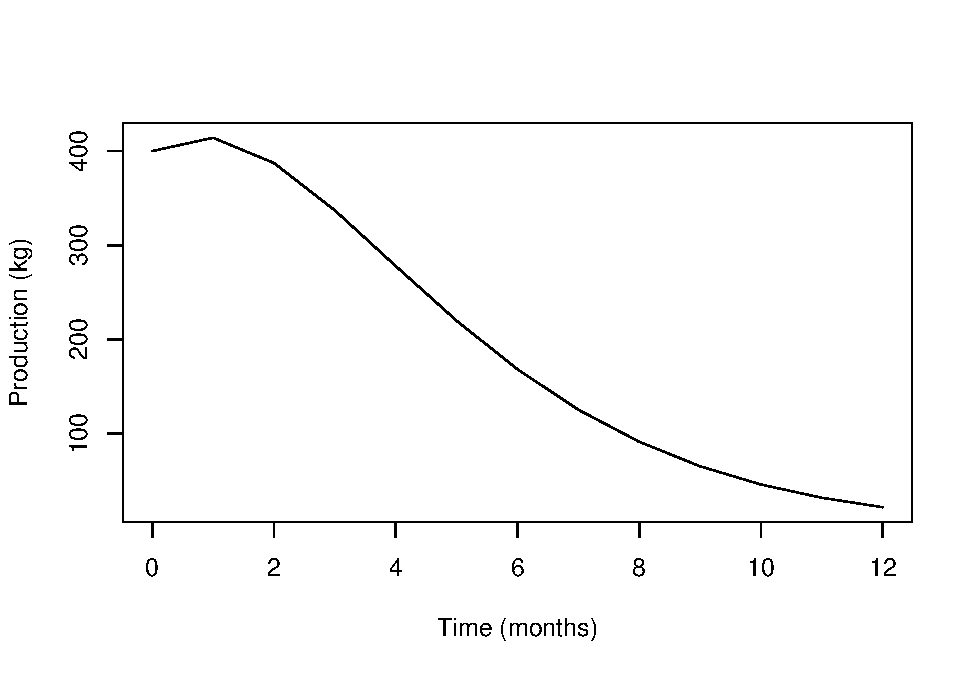
\includegraphics{Physical_Processes_In_Ecosystems_files/figure-latex/unnamed-chunk-6-1.pdf}

3a. The rate of change of \(N\) is a decrease (i.e.~negative) and proportional to \(N\). For \(k > 0\), we have \(\frac{dN}{dt}=-kN\).

\begin{enumerate}
\def\labelenumi{\alph{enumi}.}
\setcounter{enumi}{1}
\item
  Separate variables
  \[\frac{dN}{N}=-kdt\]
  \[\int \frac{dN}{N}= \int -kdt\]
  \(\ln N= -kt+C\), \(C\) = integration constant
  \[N= e^{-kt}e^{C}\]
  But \(N(0)=N_0\). Thus \(N(0)=N_0=e^0 e^C=e^C\)
  and the solution is \(N(t)= N_0e^{-kt}\).
\item
  Substitute into the solution equation.
  \begin{align*}
  N(t_1)=N_0e^{-kt_1} \\
  0.5 N_0= N_0e^{-kt_1}  \\
  \ln(0.5)=-kt_1 \\
  t_1= -(\ln(0.5))/k \\
  = (\ln 2)/k
  \end{align*}
\item
  Let N(t) be the number of \(C^{14}\) atoms in the wood. Then \(N(t)/N_0 = 0.87\). The half life of 5568 gives \((\ln2)/k=5568\), \(k= (\ln 2)/5568=0.0001245\).
  The equation for N(t) then gives
  \begin{align*}
  N(t)/N_0=e^{-kt} \\
  0.87 = exp(-0.0001245t)\\
  \ln(0.87) = -0.0001245t\\
  t=1119 years
  \end{align*}
\end{enumerate}

\begin{enumerate}
\def\labelenumi{\arabic{enumi}.}
\setcounter{enumi}{3}
\tightlist
\item
  a is the amplitude (half the total change in tidal height); b is \(2\pi/p\) where p=period=\(2|T_{high}-T_{low}|\); and \(T_h\) is the phase shift or lag. The simple cosine function begins at \(t=0\) so the lag is the time of high tide. \(H_a\) is the vertical shift.
\end{enumerate}

\begin{Shaded}
\begin{Highlighting}[]
\CommentTok{\#first interval}
\NormalTok{h\_h=}\StringTok{ }\FloatTok{2.47}
\NormalTok{h\_l=}\StringTok{ }\FloatTok{{-}0.82}
\NormalTok{time\_h=}\StringTok{ }\DecValTok{4}\OperatorTok{+}\DecValTok{35}\OperatorTok{/}\DecValTok{60}
\NormalTok{time\_l=}\StringTok{ }\DecValTok{11}\OperatorTok{+}\DecValTok{40}\OperatorTok{/}\DecValTok{60}

\CommentTok{\#second interval}
\NormalTok{h\_h=}\StringTok{ }\FloatTok{2.77}
\NormalTok{h\_l=}\StringTok{ }\FloatTok{{-}0.82}
\NormalTok{time\_h=}\StringTok{ }\DecValTok{19}\OperatorTok{+}\DecValTok{40}\OperatorTok{/}\DecValTok{60}
\NormalTok{time\_l=}\StringTok{ }\DecValTok{11}\OperatorTok{+}\DecValTok{40}\OperatorTok{/}\DecValTok{60}
  
\NormalTok{a=}\StringTok{ }\NormalTok{(h\_h}\OperatorTok{{-}}\NormalTok{h\_l)}\OperatorTok{/}\DecValTok{2}
\NormalTok{p=}\StringTok{ }\DecValTok{2}\OperatorTok{*}\KeywordTok{abs}\NormalTok{(time\_h}\OperatorTok{{-}}\NormalTok{time\_l)}
\NormalTok{b=}\DecValTok{2}\OperatorTok{*}\NormalTok{pi}\OperatorTok{/}\NormalTok{p}
\NormalTok{time\_h=}\StringTok{ }\NormalTok{time\_h }\CommentTok{\#phase lag, time of high tide}
\NormalTok{Ha=}\StringTok{ }\NormalTok{(h\_h}\OperatorTok{+}\NormalTok{h\_l)}\OperatorTok{/}\DecValTok{2}

\NormalTok{a; p; b; time\_h; Ha}
\end{Highlighting}
\end{Shaded}

\begin{verbatim}
## [1] 1.795
\end{verbatim}

\begin{verbatim}
## [1] 16
\end{verbatim}

\begin{verbatim}
## [1] 0.3926991
\end{verbatim}

\begin{verbatim}
## [1] 19.66667
\end{verbatim}

\begin{verbatim}
## [1] 0.975
\end{verbatim}

\begin{Shaded}
\begin{Highlighting}[]
\NormalTok{H=}\ControlFlowTok{function}\NormalTok{(a,b,time, time\_h, Ha) a}\OperatorTok{*}\KeywordTok{cos}\NormalTok{(b}\OperatorTok{*}\NormalTok{(time}\OperatorTok{{-}}\NormalTok{time\_h))}\OperatorTok{+}\NormalTok{Ha}
\KeywordTok{plot}\NormalTok{(}\DecValTok{1}\OperatorTok{:}\DecValTok{24}\NormalTok{, }\KeywordTok{H}\NormalTok{(}\DataTypeTok{a=}\NormalTok{a,}\DataTypeTok{b=}\NormalTok{b,}\DataTypeTok{time=}\DecValTok{1}\OperatorTok{:}\DecValTok{24}\NormalTok{, }\DataTypeTok{time\_h=}\NormalTok{time\_h, }\DataTypeTok{Ha=}\NormalTok{Ha), }\DataTypeTok{type=}\StringTok{\textquotesingle{}l\textquotesingle{}}\NormalTok{, }
     \DataTypeTok{xlab=}\StringTok{"Tide height (m)"}\NormalTok{, }\DataTypeTok{ylab=}\StringTok{"Time (hours)"}\NormalTok{)}
\end{Highlighting}
\end{Shaded}

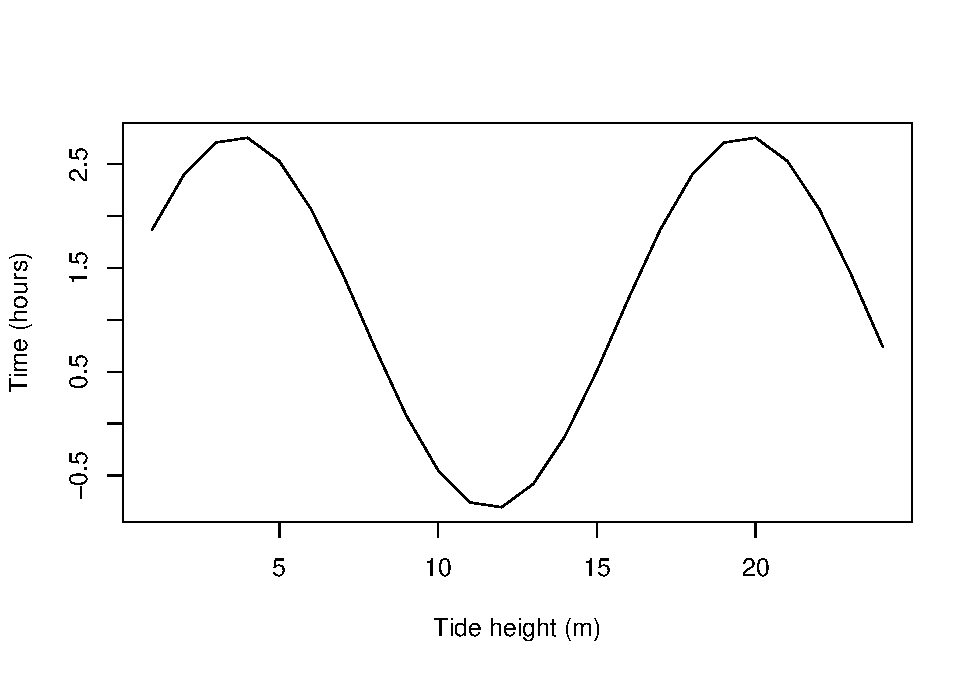
\includegraphics{Physical_Processes_In_Ecosystems_files/figure-latex/unnamed-chunk-7-1.pdf}
b. \(\overline H\)= average height, first interval = 7.24 hours.
\begin{align*}
\overline H&= \frac{1}{7.24} \int^{11.82}_{4.58}a \cos(bT-bT_h)+H_a dt \\
&= \frac{1}{7.24} (-a/b)(\sin(11.82b-4.58b)-sin(4.58b-4.58b)) + \frac{1}{7.24} (H_a)(11.82-4.58)\\
&=-\frac{a}{7.24b}(\sin(7.24(2\pi/2(7.24)))-0)+H_a\\
&=H_a \text{, since } \sin \pi=0.
\end{align*}

For the two intervals combined, we must weight the average height in each interval by the length of the time interval.
\begin{align*}
\overline H&= \frac{1}{15.09} \int^{19.67}_{4.58}H(t)dt=\frac{1}{15.09}\int^{11.82}_{4.58}H(t)dt +\frac{1}{15.09}\int^{19.67}_{11.82}H(t)dt\\
&=\frac{7.24}{15.09}\frac{1}{7.24}\int^{11.82}_{4.58}H(t)dt +\frac{7.85}{15.09}\frac{1}{7.85}\int^{19.67}_{11.82}H(t)dt\\
&=\frac{7.24}{15.09} \overline H_1 +\frac{7.85}{15.09} \overline H_2\\
\end{align*}

\begin{enumerate}
\def\labelenumi{\alph{enumi}.}
\setcounter{enumi}{2}
\tightlist
\item
  We need the times of day when the 0.0 tide level is reached. The easiest way is to invert the function \(H(t)\) for each subinterval.
  \begin{align*}
  &H= a \cos(b(T-T_h))+H_a\\
  &(H-H_a)/a= \cos(b(T-T_h))\\
  &\cos^{-1}((H-H_a)/a)=b(T-T_h)\\
  &(1/b) \cos^{-1}((H-H_a)/a)+T_h=T\\
  \end{align*}
  Now substitute the appropriate constants and 0 for \(H\).
\end{enumerate}

\begin{Shaded}
\begin{Highlighting}[]
\CommentTok{\#first interval}
\NormalTok{h\_h=}\StringTok{ }\FloatTok{2.47}
\NormalTok{h\_l=}\StringTok{ }\FloatTok{{-}0.82}
\NormalTok{time\_h=}\StringTok{ }\DecValTok{4}\OperatorTok{+}\DecValTok{35}\OperatorTok{/}\DecValTok{60}
\NormalTok{time\_l=}\StringTok{ }\DecValTok{11}\OperatorTok{+}\DecValTok{40}\OperatorTok{/}\DecValTok{60}

\CommentTok{\#second interval}
\NormalTok{h\_h=}\StringTok{ }\FloatTok{2.77}
\NormalTok{h\_l=}\StringTok{ }\FloatTok{{-}0.82}
\NormalTok{time\_h=}\StringTok{ }\DecValTok{19}\OperatorTok{+}\DecValTok{40}\OperatorTok{/}\DecValTok{60}
\NormalTok{time\_l=}\StringTok{ }\DecValTok{11}\OperatorTok{+}\DecValTok{40}\OperatorTok{/}\DecValTok{60}
  
\NormalTok{a=}\StringTok{ }\NormalTok{(h\_h}\OperatorTok{{-}}\NormalTok{h\_l)}\OperatorTok{/}\DecValTok{2}
\NormalTok{p=}\StringTok{ }\DecValTok{2}\OperatorTok{*}\KeywordTok{abs}\NormalTok{(time\_h}\OperatorTok{{-}}\NormalTok{time\_l)}
\NormalTok{b=}\DecValTok{2}\OperatorTok{*}\NormalTok{pi}\OperatorTok{/}\NormalTok{p}
\NormalTok{time\_h=}\StringTok{ }\NormalTok{time\_h }\CommentTok{\#phase lag, time of high tide}
\NormalTok{Ha=}\StringTok{ }\NormalTok{(h\_h}\OperatorTok{+}\NormalTok{h\_l)}\OperatorTok{/}\DecValTok{2}

\NormalTok{H=}\DecValTok{0}

\CommentTok{\#Estimate T}
\NormalTok{(}\DecValTok{1}\OperatorTok{/}\NormalTok{b)}\OperatorTok{*}\KeywordTok{acos}\NormalTok{((H}\OperatorTok{{-}}\NormalTok{Ha)}\OperatorTok{/}\NormalTok{a)}\OperatorTok{+}\NormalTok{time\_h}
\end{Highlighting}
\end{Shaded}

\begin{verbatim}
## [1] 25.12889
\end{verbatim}

This answer is obviously wrong since the 0.0 height must be attained sometime between low tide (11.82 hours) and the next high tide (19.67 hours). The fallacy is in treating the ``arcos x'' as an inverse function. It is one-to-one only when the domain of ``cos x'' is restricted to \([0,\pi]\); i.e., arcos x always has \([0,\pi]\) as its range. Thus the first term is
\[\frac{1}{0.400}\cos^{-1}(-0.975/1.795)\]
correctly tells how far the maximum (\(T_h\)) is from the desired time \(T\), but now whether \(T\) lies above or below \(T_h\). With the second subinterval, \(T\) is obviously below \(T_h\) and hence we subtract from \(T_h\):

\begin{Shaded}
\begin{Highlighting}[]
\FloatTok{19.67}\DecValTok{{-}1}\OperatorTok{/}\FloatTok{0.400}\OperatorTok{*}\KeywordTok{acos}\NormalTok{(}\OperatorTok{{-}}\FloatTok{0.975}\OperatorTok{/}\FloatTok{1.795}\NormalTok{)}
\end{Highlighting}
\end{Shaded}

\begin{verbatim}
## [1] 14.30747
\end{verbatim}

\begin{enumerate}
\def\labelenumi{\arabic{enumi}.}
\setcounter{enumi}{4}
\tightlist
\item
\end{enumerate}

\begin{align*}
\frac{\partial E}{\partial B} &=\sum^n_{i=1}2[Ax_i+B-y_i] \\
E&= \sum^n_{i=1}[Ax_i+B-y_i]^2\\
\frac{\partial E}{\partial A} &= \sum^n_{i=1}[Ax_i+B-y_i]x_i\\
\end{align*}
Set equal to zero:
\begin{align}
\sum^n_{i=1}2[Ax_i+B-y_i]x_i=0 \notag \\
\sum^n_{i=1}[Ax_i+B-y_i]x_i=0 \notag \\
\frac{\partial E}{\partial B} =\sum^n_{i=1}2[Ax_i+B-y_i]
\label{eq:calcint-a}
\end{align}

Equate to 0 and divide by 2:
\begin{equation}
\sum^n_{i=1}[Ax_i+B-y_i]=0
\label{eq:calcint-b}
\end{equation}
Thus we have two equations which are linear in A and B. This is more easily seen if we rework them. From (\eqref{eq:calcint-a})

\begin{equation}
A(\sum^n_{i=1}x_i^2)+B(\sum^n_{i=1}x_i)-(\sum^n_{i=1}x_iy_i)=0
\label{eq:calcint-a2}
\end{equation}

And (\eqref{eq:calcint-b}) becomes
\begin{equation}
A(\sum^n_{i=1}x_i^2)+nB-(\sum^n_{i=1}y_i)=0
\label{eq:calcint-b2}
\end{equation}

\begin{enumerate}
\def\labelenumi{\arabic{enumi}.}
\setcounter{enumi}{5}
\tightlist
\item
\end{enumerate}

\begin{enumerate}
\def\labelenumi{\alph{enumi}.}
\tightlist
\item
  Eq. \eqref{eq:calcint-a2} is:
  \[A(1353.25) + B(65.90) - (3750.50) = 0\]
  Eq. \eqref{eq:calcint-b2} is:
  \[A(65.90) + 5B - (268.50) = 0\]
\end{enumerate}

We solve for A and B.

\begin{align*}
B &= (268.50 - 65.90A)/5 \\
A &= (3750.50 - 65.90B)/(1353.25) \\
&= 2.771 - 2.615 + 0.642A = 0.156 + 0.642A \\
\end{align*}

Thus

\begin{align*}
A &= 0.156/(1 - 0.642) = 0.436 \\
B &= (268.50 - 65.90(0.436))/5 = 47.95 \\
\end{align*}

To prove that these values for \(A\), \(B\) do give a minimum sum of
squares, we must show that, for \(A\) = 0.44, \(B\) = 47.95,

\begin{enumerate}
\def\labelenumi{\roman{enumi})}
\tightlist
\item
  \(\partial f/\partial A=\partial f/\partial B = 0\)
\item
  \((\partial^2f/\partial A^2)(\partial^2f/\partial B^2)-(\partial^2f/\partial A\partial B)^2 > 0\)
\item
  \(\partial^2f/\partial A^2 > 0\),
\end{enumerate}

where \(f\) is the sum of squares
\[f=\sum_i(y_i-Ax_i-B)^2\]
We have
\begin{align*}
\partial f/\partial A &= -2\sum_i(y_i-Ax_i-B)x_i \\
\partial f/\partial B &= -2\sum_i(y_i-Ax_i-B) \\
\end{align*}

Since \(A\), \(B\) were calculated by setting these derivatives to zero, we do not need to check (i).
\begin{align*}
\partial^2f/\partial A^2 &= 2\sum_ix^2_i,\;\;\partial^2f/\partial B^2 = 2n \\
\partial^2f/\partial A\partial B &= 2 \sum_ix_i \\
\end{align*}

Substituting into (ii) gives
\[(2\sum_ix^2_i)(2n)-4(\sum_ix_i)^2=20\sum_ix^2_i-4(\sum_ix_i)^2\]
\[ = 20(1353.25) - 4(65.90)^2\]
\[=9693.76 > 0\]
Note that (iii) is obviously satisfied so we have a minimum for \(f\).

\begin{enumerate}
\def\labelenumi{\alph{enumi}.}
\setcounter{enumi}{1}
\tightlist
\item
  Begin with
  \[y = Axe^{Bx}\]
  Divide by \(x\) to isolate the exponential function.
  \[y/x=Ae^{Bx}\]
  Now take logarithms of both sides.
  \[ln(y/x)=lnA+Bx\]
  Thus, in the form \(h=f+gx\), we have
  \begin{align*}
  h &= ln(y/x) \\
  f &= ln A \\
  g &= B \\
  \end{align*}
\end{enumerate}

The transformed table is below.

\begin{longtable}[]{@{}cc@{}}
\toprule
\(x\) & \(h\)\tabularnewline
\midrule
\endhead
3.0 & 2.565\tabularnewline
5.3 & 2.340\tabularnewline
9.6 & 1.790\tabularnewline
18.0 & 1.204\tabularnewline
30.0 & 0.642\tabularnewline
\bottomrule
\end{longtable}

The least squares calculations give the transformed equation

\[h = 2.642 - 0.071x\]

and thus

\[y = 14.041x e^{-0.071x}\]

\begin{enumerate}
\def\labelenumi{\alph{enumi}.}
\setcounter{enumi}{2}
\tightlist
\item
  The following graph (fig.~4A) compares the least squares line and exponential curve of parts (a) and (b) with the data and the exponential curve in the text (eqn. \eqref{eq:calcint-12}). The fit of eqn. (\eqref{eq:calcint-12}) seems superior to that of the curve from (b).
  However, the fit of
\end{enumerate}

\[h = 2.642 - 0.071x\]

to the transformed data is quite good, as shown by fig.~5A. Thus we conclude that a good least squares fit to transformed data does not necessarily imply a good curve fit to the original data.

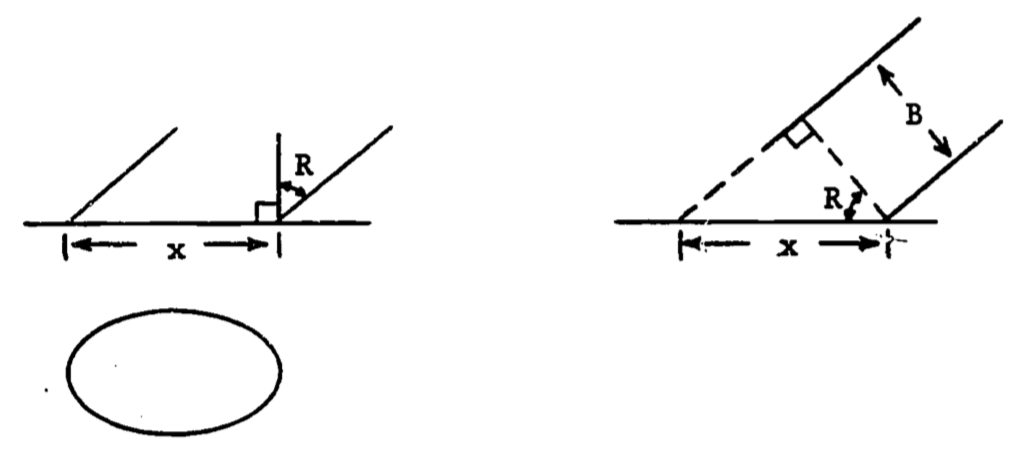
\includegraphics[width=0.75\linewidth]{figures/fig-calcint-p72}

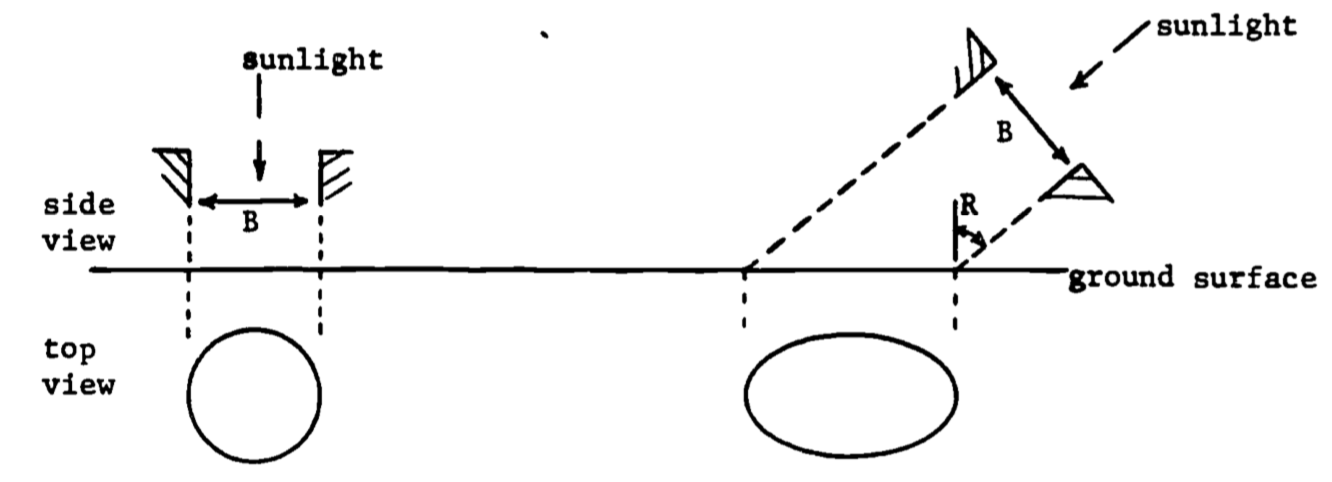
\includegraphics[width=0.75\linewidth]{figures/fig-calcint-p69}

\hypertarget{additional-problems}{%
\section{ADDITIONAL PROBLEMS}\label{additional-problems}}

\begin{enumerate}
\def\labelenumi{\arabic{enumi}.}
\tightlist
\item
  One way to use least-squares is to approximate one function by another. Here we approximate the curve
  \[y = 6.1(x+5.0)e^{-0.045x}\]
  by a straight line
  \[ y = Ax + B\]
\end{enumerate}

Evaluate both \(\partial (E^2)/\partial A\) and \(\partial (E^2)/\partial B\), then set both equal to zero to obtain two equations in A and B. The goal is to minimize:
\[E^2 = \int^{30}_3[6.1(x+5.0)e^{-0.045x}-Ax-B]^2dx\]
(Hint: when evaluating \(\partial E^2/\partial A\) and \(\partial E^2/\partial B\), differentiate under the integral sign.)

Solve your equations for A and B and the least squares integral.

\begin{enumerate}
\def\labelenumi{\arabic{enumi}.}
\setcounter{enumi}{1}
\tightlist
\item
  The stomates in leaves are small pores which permit the exchange of gases and water vapor. The stomates change shape from a near circle to a slit in order to adjust this exchange in response to varying environmental conditions. Each stomate is roughly elliptical in shape with constant perimeter throughout the shape change. The area of the opening is then given by
  \[A= \frac{2b}{a}\int^a_{-a}(a^2-x^2)^{1/2}dx\]
  where \(2a\), \(2b\) are the lengths of the major and minor axes, respectively, of the ellipse.
\end{enumerate}

\begin{enumerate}
\def\labelenumi{\alph{enumi}.}
\item
  First evaluate this integral using either of two trigonometric substitutions: let \(x = a cos \theta\) or let \(x = a sin \theta\). Be sure to check the limits on \(\theta\) and the sign of each trig function in the transformed integrand. Your result must be non-negative since the area is non-negative. For a fixed perimeter, say \(35 \mu\), the area should be maximal when the hole is a circle, i.e.~\(a=b\). Demonstrate this by evaluating the area when \(a=b=5.57\), and when \(a=5\), \(b=6.09\). (The perimeter formula is \(P = 2\pi\sqrt{(a^2+b^2)/2}\).)
\item
  Use your area formula (the answer to part a) to investigate the dilution of the sun's energy flux due to the angle at which the rays strike the earth's surface. The dilution is caused by a fixed amount of solar energy being spread over a larger area (as the rays become more horizontal) and thus the energy per unit area decreases as compared to the energy density of vertical rays. The situation is pictured below, giving a top and side view for two inclination angles. The sunlight passes through a circular hole in an opaque sheet and strikes the earth at an angle \(R\) from the perpendicular.
\end{enumerate}

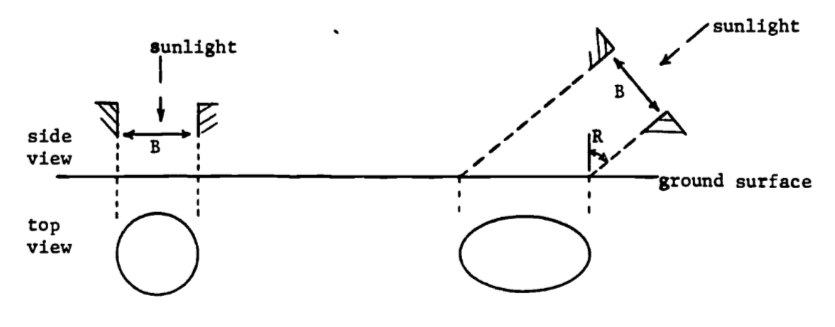
\includegraphics[width=0.75\linewidth]{figures/fig-calcint-c3}

The illuminated area changes from a circle (\(R=0\)) to an elongated ellipse (as \(R\) increases). For a given diameter \(B\), write the illuminated area \(A\) as a function of the angle of inclination \(R\). Check your result by choosing values for \(B\) and \(R\) and calculating the dilution \(D\), which equals the circle's area divided by the ellipse's area. Does \(D = 0.6\) mean more dilution (less energy density) than \(D = 0.3\) or vice versa? The inclination angle in Minnesota changes from about 20° in summer to 65° in winter. What is the resulting change in energy density, measured by \(D\)?

\hypertarget{solution-to-the-additional-problems}{%
\section{SOLUTION TO THE ADDITIONAL PROBLEMS}\label{solution-to-the-additional-problems}}

\begin{enumerate}
\def\labelenumi{\arabic{enumi}.}
\tightlist
\item
  First partial derivatives:
  \begin{align*}
  \frac{\partial E^2}{\partial A} &= \int^{30}_3\frac{\partial}{\partial A}(6.1(x+5.0)e^{-0.045x}-Ax-B)^2dx \\
  &= 2 \int^{30}_3(6.1(x+5.0)e^{-0.045x}-Ax-B)(-x)dx
  \end{align*}
  Equating to zero and dividing by 2 gives
  \[0 = -\int^{30}_36.1(x-2+5x)e^{-0.045x}dx +\int^{30}_3Ax^2+Bxdx\]
  Successive integration by parts (for the first integral) and direct integration (for the second integral) yield the first equation:
  \[0 = 8991.0A + 445.5B - 25984.9\]
  \begin{align*}
  \frac{\partial E^2}{\partial B} &= \int^{30}_3\frac{\partial}{\partial B}(6.1(x+5.0)e^{-0.045x}-Ax-B)^2dx \\
  &= -2 \int^{30}_3(6.1(x+5.0)e^{-0.045x}-Ax-B)dx
  \end{align*}
\end{enumerate}

Equating to zero, dividing by 2 and solving yields the second equation:
\[0 = 445.5A + 27.0B - 1568.8\]

The solutions are \(A= 0.061\), \(B = 57.1\). The least squares integral using the approximation \(Y = 0.061x + 57.1\)
is 546.452.

\begin{enumerate}
\def\labelenumi{\arabic{enumi}.}
\setcounter{enumi}{1}
\tightlist
\item
\end{enumerate}

\begin{enumerate}
\def\labelenumi{\alph{enumi}.}
\tightlist
\item
  Let \(x=a\:sin\theta\). The limits of integration are then changed as follows
  \[-a \le x \le a\]
  \[ -a \le asin\theta \le a\]
  \[ -1 \le sin\theta \le 1\]
\end{enumerate}

There are many options for the range of \(\theta\). We first change the integrand to see which range is suitable. We know the integrand is non-negative since \(x^2 \le a^2\). Substitution gives
\[x = asin\theta\]
\[dx = acos\theta\:d\theta\]
\[\sqrt{a^2-x^2}dx = \sqrt{a^2 - a^2sin^2\theta}\cdot acos\theta \:d\theta\]
The integrand is then non-negative when the positive square root is used and when \(cos \theta\) is non-negative. Thus, we choose the limits of integration to be \(-\frac{\pi}{2}\), \(\frac{\pi}{2}\) since \(sin(-\frac{\pi}{2}) = 1, sin(\frac{\pi}{2}=1)\) and \(cos\theta \le0\) if \(-\frac{\pi}{2} \le \theta \le \frac{\pi}{2}\).\\
The integral is then
\[\int^{\pi/2}_{-\pi/2}\sqrt{a^2-a^2sin^2\theta}acos\theta \:d\theta = a^2\int^{\pi/2}_{-\pi/2}\sqrt{1-sin^2\theta}cos\theta\:d\theta\]
\begin{align*}
&= a^2\int^{\pi/2}_{-\pi/2}cos^2\theta\:d\theta=a^2[\frac{\theta}{2}+\frac{sin2\theta}{4}]^{\pi/2}_{-\pi/2} \\
&= a^2[\pi/4+(1/4)(0)-(-\pi/4)-(1/4)(0)] =\pi a^2/2
\end{align*}
Thus
\[A=\frac{2b}{a}\int^a_{-a}\sqrt{a^2-x^2}dx = \pi ab\]
When \(a = b = 5.57\), \(A = 97.47\).\\
When \(a = 5\), \(b = 6.09\), \(A = 95.66\).

\begin{enumerate}
\def\labelenumi{\alph{enumi}.}
\setcounter{enumi}{1}
\tightlist
\item
\end{enumerate}

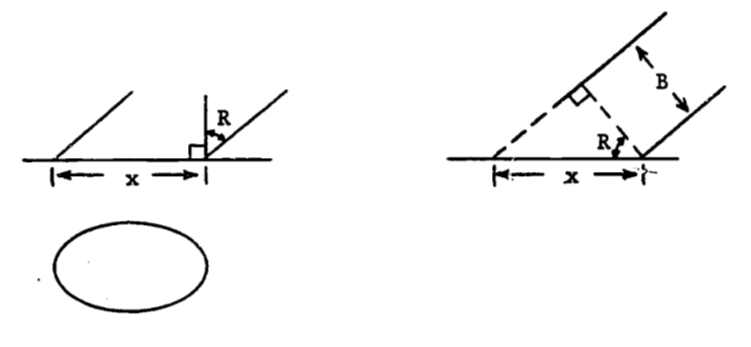
\includegraphics[width=0.75\linewidth]{figures/fig-calcint-cs3}

From the right-hand diagram, we have
\[cosR = B/x\]
and thus
\[x=B/cosR\]
The minor axis is then the circle's diameter, \(B\). In the answer to part ``a'', we replace \(2a\) by \(B/cos R\) and \(2b\) by \(B\).

\begin{align*}
A &= \pi ab = \pi(B/2cosR)(B/2) \\
&= \pi B^2 / (4 cosR)
\end{align*}

Since the area of the circle is \(\pi B^2/4\),the dilution coefficient is
\[D = \frac{\pi B^2/4}{\pi B^2/4cosR} = cosR\]
Thus \(D=0.6\) means less dilution than \(D=0.3\), and \(D=1.0\) means no dilution at all. For Minnesota, the coefficients are\\
\(D=0.94\) for \(R=20°\)\\
\(D=0.42\) for \(R=65°\)

\hypertarget{calcdiff}{%
\chapter{Calculus-Differentiation.}\label{calcdiff}}

author: Hertzberg, R. H.

\hypertarget{preface-1}{%
\section{PREFACE}\label{preface-1}}

This module is used to introduce the biology student to differential calculus, a branch of mathematics that is often used in ecological and physiological models. Since biological systems are dynamic, their mathematical models must describe rates of change of relevant variables,a process which requires calculus. The module introduces modeling in biology by reviewing differential calculus and using only examples from life sciences. A problem set reviews information in the text proper and presents additional information not included in the text. The module uses computer programming to graphically check the user's own calculations and to demonstrate the validity of general solutions.

\hypertarget{introduction-1}{%
\section{INTRODUCTION}\label{introduction-1}}

Differential calculus is being used more often in recent ecological and physiological models as data become more precise and the processes become better understood. Since most biological systems are dynamic, their mathematical models must describe rates of change, not just current values, of the relevant variables. Although most models consider changes over time, the techniques of calculus depend only on the mathematical function involved and thus any independent variable may be used, such as spatial dimensions, organism weight, temperature, etc. As a result, the implications from a model of one process may be applied to the model of a different process as long as the mathematical functions involved are the same.

\hypertarget{functions-of-one-variable}{%
\section{FUNCTIONS OF ONE VARIABLE}\label{functions-of-one-variable}}

\hypertarget{rates-of-change}{%
\subsection{Rates of Change}\label{rates-of-change}}

The simplest graph of a dynamic relationship is a straight line. The equation for a straight line is

\begin{equation}
y = mx+ b
\label{eq:calcdiff-1}
\end{equation}

where \(y\) and \(x\) are variables, \(m\) and \(b\) are constants. An example of this relation is the oxygen uptake by the lobster. The oxygen consumption \((y)\) depends on the oxygen concentration \((x)\) in the surrounding environment, so that \(y\) is a function of \(x\). A typical graph of this function shown in Figure \ref{fig:fig-calcdiff-1}.

\begin{figure}
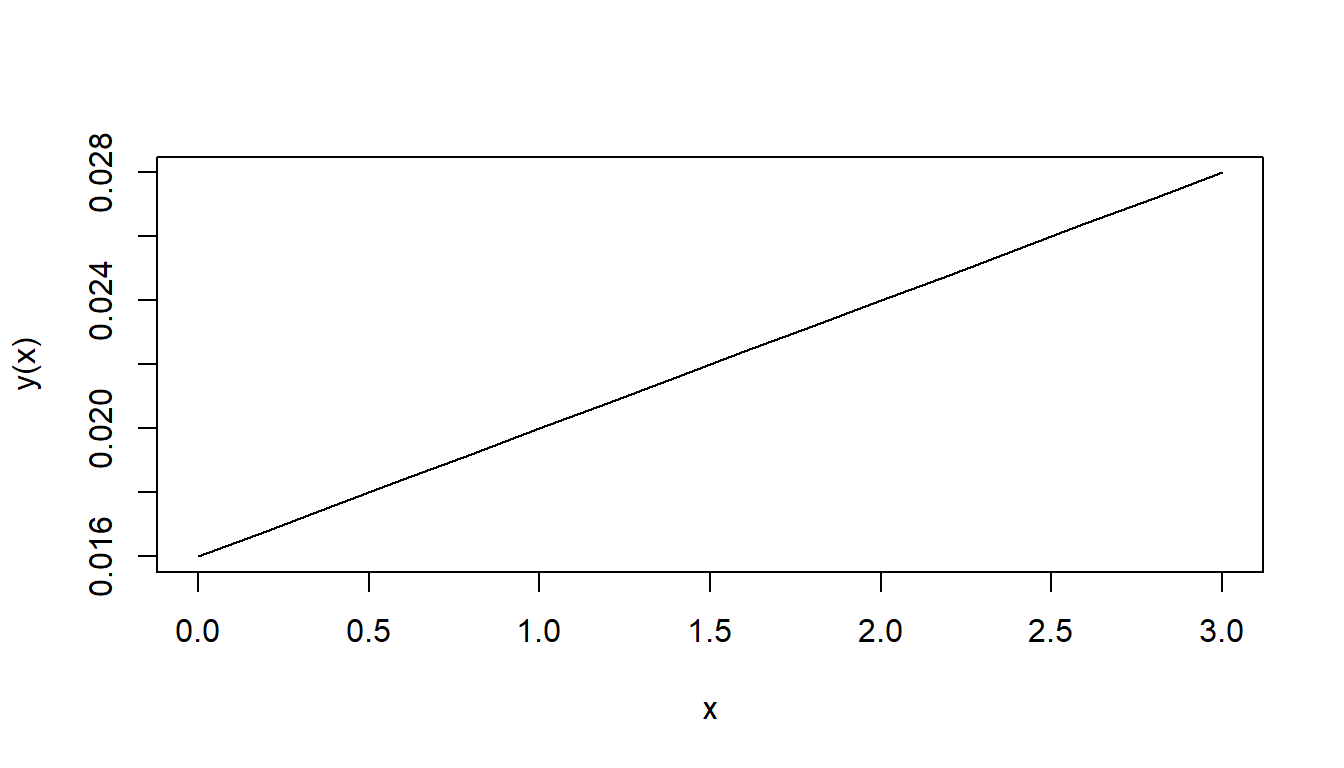
\includegraphics[width=0.75\linewidth]{Physical_Processes_In_Ecosystems_files/figure-latex/fig-calcdiff-1-1} \caption{Oxygen consumption.}\label{fig:fig-calcdiff-1}
\end{figure}

The equation for this function is
\[y(x)=0.004x+0.016\]
The number 0.004 represents the slope of the line; that is, the ratio of the change in \(y\) to the change in \(x\). When \(x\) changes by 1 unit, \(y\) changes by 0.004 units. In this particular application, when the water O\textsubscript{2} concentration increases by one ml/l, the lobster O\textsubscript{2} consumption increases by 0.004 ml per hour-gm body weight. The slope (\(m\) in Equation \eqref{eq:calcdiff-1}) then represents the rate of change of \(y\) with \(x\).

When the graph is not a straight line, the function it represents is more complex than above and the rate of change cannot be expressed so easily. Note that for each unit change in \(x\) in Fig. \ref{fig:fig-calcdiff-1}, \(y\) changes by 0.004, regardless of the value of \(x\). The rate of change is then constant. In the graph of Fig. \ref{fig:fig-calcdiff-2}, the rate of change is not constant. To see this, approximate Fig. \ref{fig:fig-calcdiff-2} by two connected tangent lines (Fig. \ref{fig:fig-calcdiff-3}a) and note that the slope differs with each line. As the approximation improves (Fig. \ref{fig:fig-calcdiff-3}b), it uses more lines and thus presents more slopes. Using an infinite number of lines, we would duplicate the curve (in Fig. \ref{fig:fig-calcdiff-2}) and have a slope that changes with each value of \(x\). The slope then depends on \(x\) and clearly is not constant. In fact, one definition of the slope of a curve at a point is the slope of the tangent line at that point.

Note that the slope is ambiguous at the points where two straight lines meet (Figure \ref{fig:fig-calcdiff-3}a). We say the slope is ``undefined'' at such ``corner'' points.

\begin{figure}
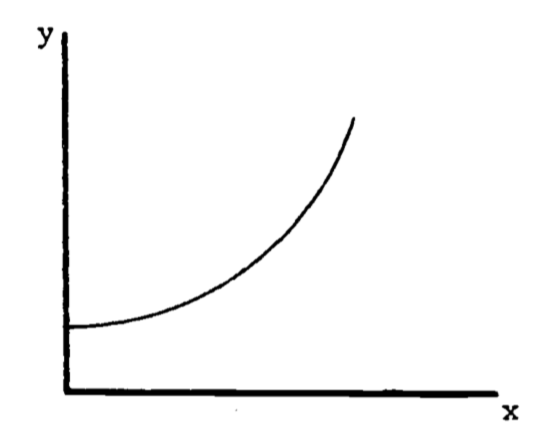
\includegraphics[width=0.5\linewidth]{figures/fig-calcdiff-2} \caption{Example of a function with a changing slope.}\label{fig:fig-calcdiff-2}
\end{figure}

\begin{figure}
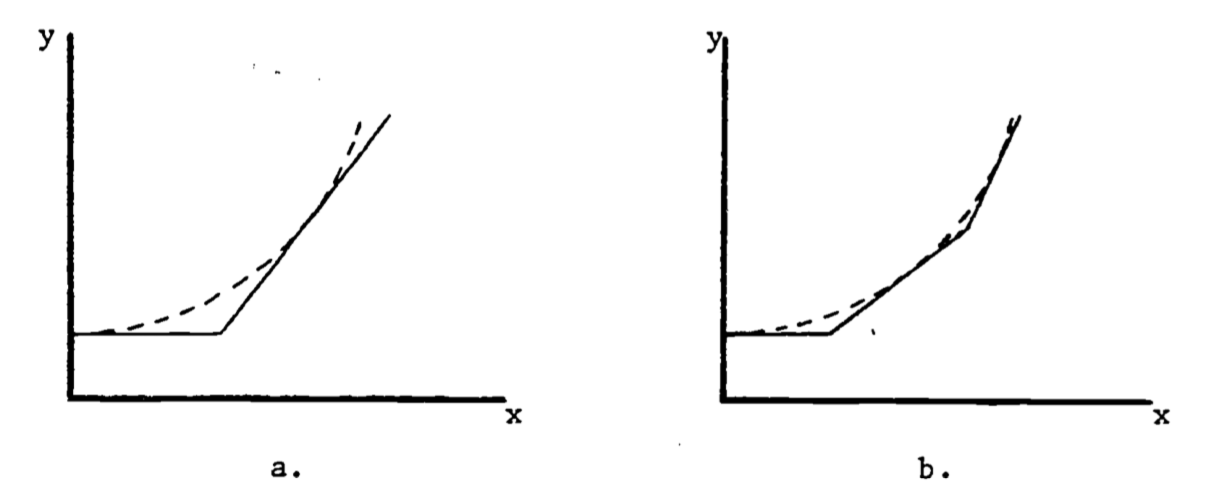
\includegraphics[width=0.75\linewidth]{figures/fig-calcdiff-3} \caption{Approximations to the curve in Figure 2.}\label{fig:fig-calcdiff-3}
\end{figure}

In general, the rate of change of a function is also a function of \(x\) and possesses its own equation. The rate of change is denoted to \(\frac{dy}{dx}\) reflect the ratio of the change in \(y\) to the change in \(x\). When the graph is a straight line, the equation for \(y\) is
\[y(x) = mx + b\]
and the rate of change is
\[\frac{dy}{dx}=m\]
The rate of change is called the \textbf{derivative}. Its functional form depends on the equation for \(y\). For example, an empirical relation between oxygen consumption \((Q)\) and body weight \((W)\) is
\[Q=3W^2\]
The derivative of this function is
\[\frac{dQ}{dW}=(3)(2W)=6W\]
The graph of \(Q = 3W^2\) is given in Fig. \ref{fig:fig-calcdiff-4}a. The derivative at \(W = 1\) represents the slope of the line tangent to the curve at the point where \(W = 1\), as shown in Figure 4b. At \(W = 1\), the slope is calculated to be
\[\frac{dQ}{dW}=6(1)=6\]

\begin{figure}
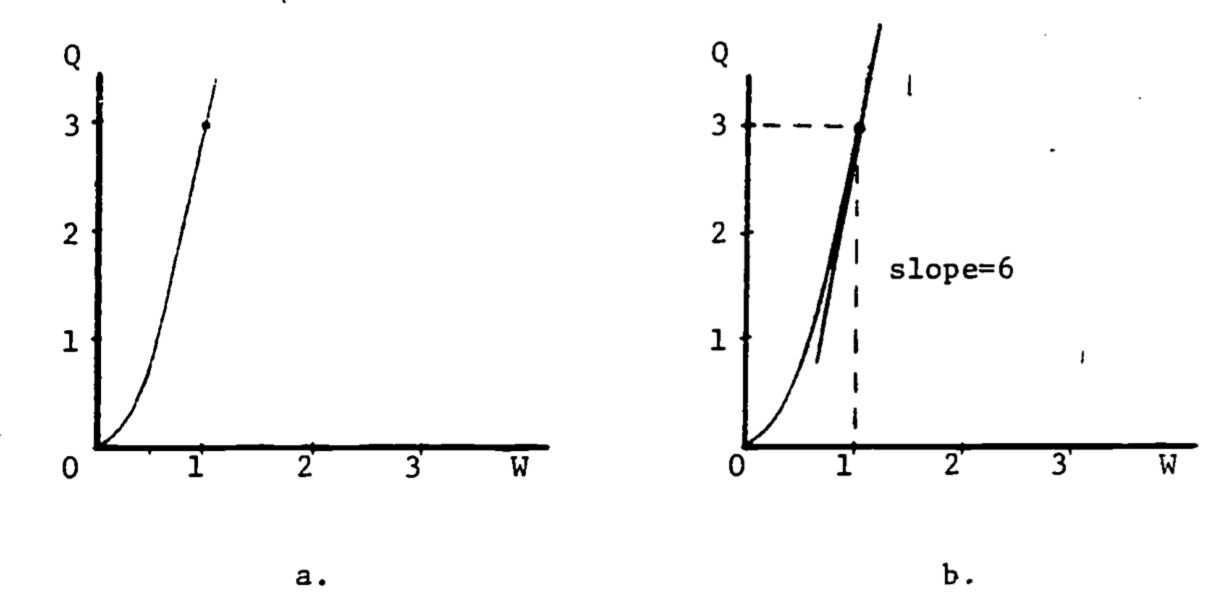
\includegraphics[width=0.75\linewidth]{figures/fig-calcdiff-4} \caption{Derivative as the slope of the tangent line.}\label{fig:fig-calcdiff-4}
\end{figure}

The number ``\(3\)'' in the formula \(Q = 3W^2\), as well as the ``\(2\)'' in the exponent, are empirically determined and differ with body size and species. The general formula is
\begin{equation}
Q=aW^b
\label{eq:calcdiff-2}
\end{equation}
The derivative of this power function is
\[\frac{dQ}{dW}=a\cdot b\cdot W^{b-1}\]
Table 1 gives the more common functions and their derivatives. For a more complete table, see any calculus text, or any math handbook (see Bibliography).

\begin{quote}
Table 1. Derivatives of Elementary Functions
\end{quote}

\begin{longtable}[]{@{}cc@{}}
\toprule
\(y(x)\) & \(dy/dx\)\tabularnewline
\midrule
\endhead
\(x^n\) & \(nx^{n-1}\)\tabularnewline
\(e^x\) & \(e^x\)\tabularnewline
\(ln\:x\) & \(1/x\)\tabularnewline
sin \(x\) & cos \(x\)\tabularnewline
cos \(x\) & -sin \(x\)\tabularnewline
\bottomrule
\end{longtable}

\hypertarget{composite-functions}{%
\subsection{Composite Functions}\label{composite-functions}}

When a function is composed of several simple functions its derivative can be evaluated in stages. In the simple cases where \(y\) equals the sum or product of two functions, \(f(x)\), \(g(x)\), the rules for differentiation (finding the derivative) are:
\[y(x)=f(x)+g(x),\;\;\;\;\frac{dy}{dx}=\frac{df}{dx}+\frac{dg}{dx}\]
\[y(x)=f(x)g(x),\;\;\;\;\frac{dy}{dx}=f(x)\frac{dg}{dx}+g(x)\frac{df}{dx}\]
For example, if \(y(x)=x^2(x-1)+2x\), then
\begin{align*}
\frac{dy}{dx}&=x^2\frac{d(x-1)}{dx}+(x-1)\frac{d(x^2)}{dx}+2 \\
&= x^2(1)+(x-1)(2x)+2 \\
\end{align*}
When \(y\) is a function of a function, the \textbf{chain rule} provides the differentiation method:
\[\frac{dy}{dx}=\frac{dy}{du}\frac{du}{dx}\]
For the composite exponential function \(y=e^{2x}\), we have
\[u(x)=2x,\;\;\;\;y(u)=e^u\]
\[\frac{dy}{du}=e^u, \;\;\;\;\frac{du}{dx}=2\]
Therefore
\[\frac{dy}{dx}=2e^u=2e^{2x}\]
The Gompertz growth curve is used occasionally to describe the population size \((N)\) of some species as a function of time \((t)\), and is given by the equation
\[N(t)=ae^{-be^{-kt}}\]
where \(a\), \(b\), \(k\) are constants. The derivative \(dN/dt\) then represents the rate of growth of the population. Here the chain rule is applied twice:
\[N(t)=ae^{u(t)},\;\;\;\;u(t)=-be^{-kt}\]
\[\frac{dN}{du}=ae^u\]
Write \(u(t)\) as \(u=-be^{v(t)}\) where \(v=-kt\). Then
\[\frac{dv}{dt}=-k,\;\;\;\;\frac{du}{dt}=\frac{du}{dv}\frac{dv}{dt}=-be^v(-k)\]
\[\frac{dN}{dt}=\frac{dN}{du}\frac{du}{dv}\frac{dv}{dt}=ae^u(-be^v)(-k)=abke^{-be^{-kt}}\cdot e^{-kt}\]

\hypertarget{higher-derivatives}{%
\subsection{Higher Derivatives}\label{higher-derivatives}}

The derivative \(dy/dx\) of a function \(y(x)\) is called the \textbf{first derivative} of \(y(x)\). If we write
\[\frac{dy}{dx}=g(x)\]
then differentiating \(g(x)\) produces
\[\frac{dg}{dx}=h(x)\]
which is called the \textbf{second derivative} of \(y(x)\), and is written \(\frac{d^2y}{dx^2}\).

Other notation used for the first derivative includes \(y'\) and \(\dot{y}\), for the second derivative, \(y''\) and \(\ddot{y}\). Since the second derivative is also a function, it too can be differentiated to give the third derivative, and so on. The \(n^{th}\) derivative is written (there is no general dot notation)
\[\frac{d^ny}{dx^n},\;\;\;\; y^{[n]}\]

\hypertarget{critical-points}{%
\subsection{Critical Points}\label{critical-points}}

The first and second derivatives can be used to determine three special points on the graph of the function, namely, the relative maxima, relative minima and the inflection points. The relative maximum is easily visualized: the curve rises, reaches a peak, and then falls. The peak is the relative maximum. It is \textbf{relative} because the curve may rise even higher in a different place on the graph. Similarly, the relative minimum constitutes a low point on the curve. An inflection point is best illustrated by an example.

The logistic growth function describing population size is
\[N=N_0\frac{1+b}{a+be^{-kt}}=N_0(1+b)(1+be^{-kt})^{-1}\]
where \(k\) is a growth coefficient, \(N_o\) is the population size at \(t=0\) and \(N_0(1+b)\) represents the carrying capacity of the environment. The growth \textbf{rate} is then
\begin{align*}
\frac{dN}{dt}&=N_0(1+b)(-1)(1+be^{-kt})^{-2}(be^{-kt})(-k) \\
&=N_0(1+b)bke^{-kt}(1+be^{-kt})^{-2} \\
\end{align*}
The coefficient \(k\) is always positive. In this example, we restrict \(b\) to be greater than 1.

At a relative maximum, the tangent line is horizontal so the slope is zero. Then the maximum growth rate occurs when the derivative of the growth rate equals zero.
\[\frac{d(dN/dt)}{dt}=0\]
or equivalently,
\[\frac{d^2N}{dt^2}=0\]

\begin{figure}
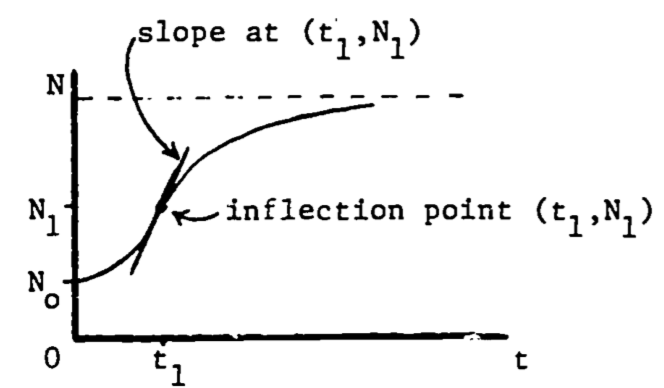
\includegraphics[width=0.75\linewidth]{figures/fig-calcdiff-5} \caption{Maximum growth rate at the inflection point.}\label{fig:fig-calcdiff-5}
\end{figure}

The second derivative of a function equals zero at the point of inflection, where the curvature changes from curving upward to curving downward, or vice versa. Then the maximum growth rate occurs when the population function \(N(t)\) is at its inflection point (see Fig. \ref{fig:fig-calcdiff-5}). Since the slope is decreasing (leveling off) \textbf{following} the inflection point, and increasing \textbf{before} the inflection point, it is certainly maximal (steepest) \textbf{at} that point. This point can also be viewed as the relative maximum on the graph of the growth rate, \(dN/dt\) (see Fig. \ref{fig:fig-calcdiff-6}).

\begin{figure}
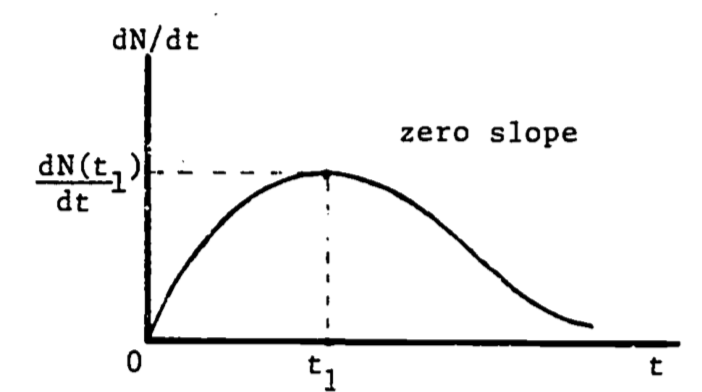
\includegraphics[width=0.75\linewidth]{figures/fig-calcdiff-6} \caption{Growth rate as a function of time.}\label{fig:fig-calcdiff-6}
\end{figure}

We now locate this point of maximum growth:
\[0=\frac{d^2N}{dt^2}\;\;\;\;\;\mbox{at } (t_1, N_1)\]
\[0=\frac{d}{dt}[N_0(1+b)bke^{-kt}(1+be^{-kt})^{-2}]\;\;\;\;\mbox{at }(t_1, N_1)\]
\[0=N_0(1+b)bk^2e^{-kt_1}(be^{-kt_1}-1)(1+be^{-kt_1})^{-3}\]
Since all factors are positive except \((be^{-kt_1}-1)\), then
\[0=be^{-kt_1}-1\]
Solving for \(t_1\) gives
\[t_1=(\frac{1}{k})ln\:b\]
and then substituting into the original expression for \(N\),
\[N_1=N_0(1+b)(1+be^{-k(\frac{1}{k}ln\,b)})^{-1}=N_0(1+b)/2\]
this says that the growth rate is highest when the population is one-half of the carrying capacity.

\hypertarget{functions-of-several-variables}{%
\section{FUNCTIONS OF SEVERAL VARIABLES}\label{functions-of-several-variables}}

\hypertarget{partial-derivatives}{%
\subsection{Partial Derivatives}\label{partial-derivatives}}

The models treated thus far involve functions of one variable. Oxygen uptake is given as a function of just the surrounding oxygen concentration. The population size depends only on time. A more complicated model, however, may involve many variables. Growth certainly depends on available food supply in addition to time. Oxygen consumption also depends on more factors than ambient oxygen concentration. One such model is discussed by Bayne, Thompson and Widdows (1973).

The model begins with the equation
\begin{equation}
\frac{dC}{dt}=aW^b
\label{eq:calcdiff-3}
\end{equation}

where \(C\) is the amount of oxygen consumed up to time \(t\), and \(a\), \(b\) and \(W\) are constants. The notation \(dC/dt\) demands that we may be able to consider \(C\) \textbf{only} as a function of \(t\). This is not always the case. Bayne, et al., studied mussels (\emph{Mytilus}) with regard to the effects of food and temperature on oxygen consumption. One of their data sets gives values for the coefficients \(a\) and \(b\) for winter vs.~summer at two activity levels:

\begin{quote}
Table 2. Oxygen consumption for Mytilus edulis
\end{quote}

\begin{longtable}[]{@{}cccc@{}}
\toprule
& & \textbf{Activity} &\tabularnewline
\midrule
\endhead
Parameter & Season & standard & routine\tabularnewline
a & Winter & 1.76 & 2.66\tabularnewline
& Summer & 1.87 & 2.64\tabularnewline
b & Winter & 0.724 & 0.774\tabularnewline
& Summer & 0.67 & 0.702\tabularnewline
\bottomrule
\end{longtable}

Standard activity represents the resting state. Routine refers to the post-feeding time period where some filtration (i.e.~muscle activity) is occurring. From table 2, we recognize significant dependence of ``\(a\)'' on the level of activity and dependence of ``\(b\)'' on both activity and season. Let season and activity be denoted \(s\) and \(m\), respectively. Then, in place of ``\(a\)'' and ``\(b\)'' we write \(a(m)\) and \(b(s,m)\) to show the dependence on the variables \(m\) and \(s\). Now
\(C\), \(a\) and \(b\) are dependent variables and \(W\), \(s\), \(m\) and \(t\) are the independent variables. We must now write \eqref{eq:calcdiff-3} as
\begin{equation}
\frac{\partial C}{\partial t}=a(m)W^{b(s,m)}
\label{eq:calcdiff-4}
\end{equation}

The derivative notation is different from that in \eqref{eq:calcdiff-3} to indicate more than one independent variable. This derivative is called a \textbf{partial derivative} and represents the rate of change of \(C\) with time while all other variables are held constant. Note that by holding all of the independent variables (except \(t\)) constant, we also hold \(a\) and \(b\) constant. So this partial derivative is obtained by differentiating the function \(C\) with respect to \(t\) and treating all of the remaining independent variables as constants.

As a simple example, consider the function
\begin{equation}
y=xt^2
\label{eq:calcdiff-5}
\end{equation}
Then
\[\frac{\partial y}{\partial x}=t^2\;\;\;\mbox{(t held constant)}\]
and
\[\frac{\partial y}{\partial t}=x\cdot 2t\;\;\;\mbox{(x held constant)}\]

\begin{figure}
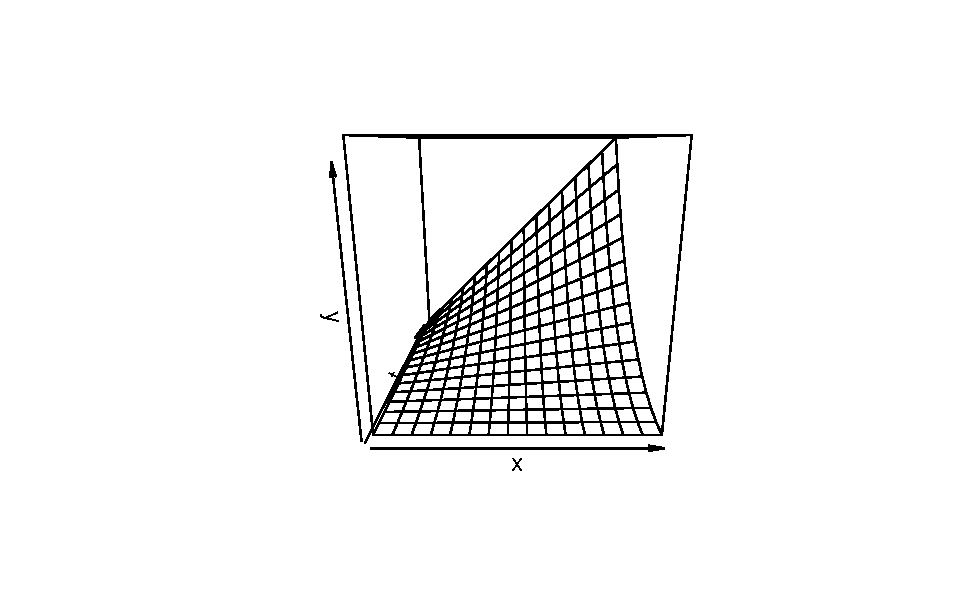
\includegraphics[width=0.75\linewidth]{Physical_Processes_In_Ecosystems_files/figure-latex/fig-calcdiff-7-1} \caption{The function $y=xt^2$.}\label{fig:fig-calcdiff-7}
\end{figure}

A partial derivative is by nature merely one simple relation (of many) extracted from a complicated function. In \eqref{eq:calcdiff-5}, when both \(x\) and \(t\) vary, the graph of \(y\) vs.~\(x\) vs.~\(t\) is a three-dimensional surface (figure \ref{fig:fig-calcdiff-7}). When \(t\) is held constant, the graph (\(y\) vs.~\(x\)) is a straight line (with slope \(t^2\) ); when \(x\) is held constant, the graph (\(y\) vs.~\(t\)) is a parabola, as shown in Figures \ref{fig:fig-calcdiff-8} and \ref{fig:fig-calcdiff-9}. These latter two graphs are much simpler than the surface of figure \ref{fig:fig-calcdiff-7}. Note that the straight line (\(y\) vs.~\(x\)) is the far edge of figure \ref{fig:fig-calcdiff-7}a, and the parabola (\(y\) vs.~\(t\)) is the near edge of figure \ref{fig:fig-calcdiff-7}c.

\begin{figure}
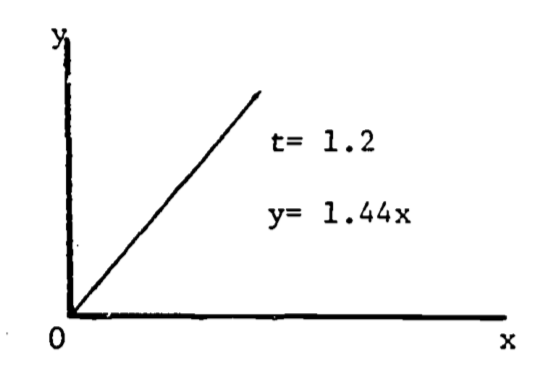
\includegraphics[width=0.75\linewidth]{figures/fig-calcdiff-8} \caption{$dy/dx=t^2$.}\label{fig:fig-calcdiff-8}
\end{figure}

\begin{figure}
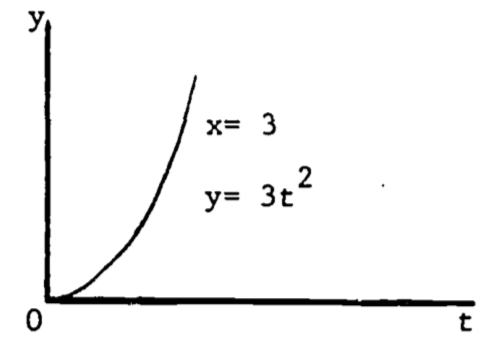
\includegraphics[width=0.75\linewidth]{figures/fig-calcdiff-9} \caption{$dy/dt=2xt$.}\label{fig:fig-calcdiff-9}
\end{figure}

A more complicated example is the complete expression for equation \eqref{eq:calcdiff-4} . The level of activity is based on the fraction of the maximal filtration rate. Then \(m=0\) represents the ``standard'' state, \(m=1\) gives the ``active'' state, and \(m=0.4\) is the ``routine'' state . Consider oxygen consumption during summer.\\
Then
\[a(m)=1.87(m+1)\]
and \eqref{eq:calcdiff-3} becomes
\begin{equation}
\frac{\partial C}{\partial t}=1.87(m+1)W^{(0.7)}
\label{eq:calcdiff-6}
\end{equation}
Changes in ``\(b\)'' are not significant so that an average value, 0.7, can be used. Since \eqref{eq:calcdiff-6} involves four variables, and thus cannot be plotted, we revert to the notation of \eqref{eq:calcdiff-2}, i.e., \(Q=\frac{\partial C}{\partial t}\). Then
\begin{equation}
Q=1.87(m+1)W^{(0.7)}
\label{eq:calcdiff-7}
\end{equation}
This last expression is similar in form to \eqref{eq:calcdiff-5} and its graph has a similar shape. Problem 3 discusses \eqref{eq:calcdiff-7} in more detail.

\hypertarget{critical-points-in-three-dimensions}{%
\subsection{Critical Points in Three Dimensions}\label{critical-points-in-three-dimensions}}

The extension of a critical point to functions of two variables is quite natural. A point \(P=(x_0,\;y_0,\;z_0)\) is a critical point for the function
\[z=f(x,y)\]
if
\[\frac{\partial f}{\partial x}=\frac{\partial f}{\partial y}=0\]
at the point \(P\). The classification of the critical point is, however, more complicated. Since there are \textbf{three} second derivatives, many cases could be considered:
\[\frac{\partial^2 f}{\partial x^2}=\frac{\partial(\partial f/\partial x)}{\partial x}\;\;\;\;\;\frac{\partial^2f}{\partial y^2}=\frac{\partial(\partial f/\partial y)}{\partial y}\]
\[\frac{\partial^2f}{\partial x\partial y}\equiv\frac{\partial(\partial f/\partial y)}{\partial x}=\frac{\partial(\partial f/\partial x)}{\partial y}\equiv\frac{\partial^2f}{\partial y\partial x}\]
This last ``mixed'' second derivative can be evaluated in either order \textbf{only if} the function \(f(x,y)\) is continuous in \(x\) and \(y\). The functions used in the examples which follow are continuous so that the order of differentiation is arbitrary. Rather than considering all combinations of sign (+, 0, -) in the second derivatives, we treat only three, which classify a relative maximum, relative minimum, and a saddle point. Define
\[L=f_{xx}(x_0,y_0)\cdot f_{yy}(x_0,y_0)-f_{xy}^2(x_0,y_0)\]
where
\[f_{xx}=\frac{\partial^2 f}{\partial x^2},\;\;\;\;\mbox{etc.}\]
P is a relative maximum if \(L > 0\) and \(f_{xx}(x_0,y_0)<0\).\\
P is a relative minimum if \(L > 0\) and \(f_{xx}(x_0,y_0)>0\).\\
P is a saddle point if \(L<0\).\\
When \(L = 0\), the situation is ``undetermined'' since its resolution is beyond the scope of this module.

An interesting example is the function
\[z=x^3+y^3-3xy+15\]
which seems to describe some of the properties of water falling across a rock face (Clow and Urquhart, 1974). Some of these properties are well known. The water will often dig potholes in the rock, especially if it falls onto a ledge. The corners and edges of the ledge eventually become rounded. We would then use a function which drops rapidly, levels off then drops steeply again. Figure \ref{fig:fig-calcdiff-10} shows a three-dimensional computer plot of this function, looking across the origin into the positive octant (\(x>0\), \(y>0\), \(z>0\)). The required shape is evident, with the pothole just beginning to form. In fact, the function does possess a relative minimum at the point \((x, y, z) = (1, 1, 14)\). This model is discussed further in problem 6.

The saddle point in the waterfall model is located at the point \((0, 0, 15)\). The region around the saddle point represents the front part of the ledge. It is displayed in the computer-drawn graph of figure \ref{fig:fig-calcdiff-11}, expanded vertically to highlight the saddle shape. Some basic features of derivatives are shown here:\\
a) The slope changes from point to point.\\
b) The slope depends on the orientation of the tangent line. Thus, at a given point, the slope found by \(\partial z/\partial x\) may be different from the slope found using \(\partial z/\partial y\).\\
c) The slope at a relative maximum or relative minimum is zero, i.e.~horizontal.

\begin{figure}
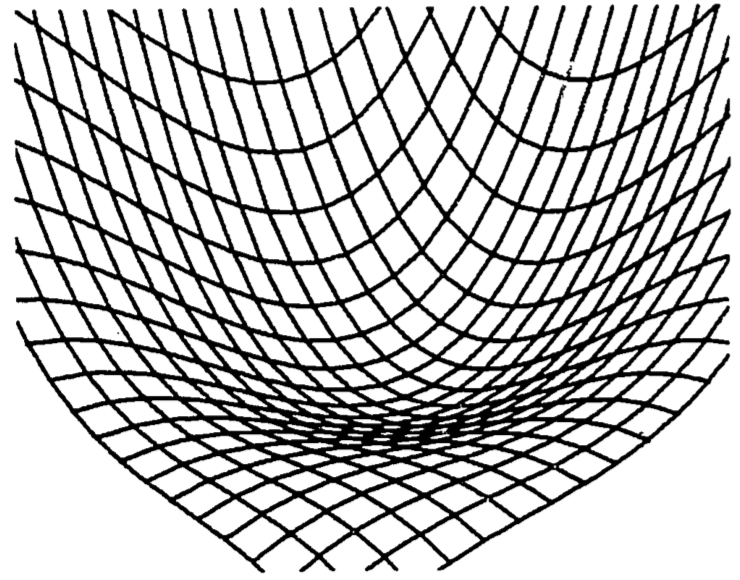
\includegraphics[width=0.4\linewidth]{figures/fig-calcdiff-10} \caption{Waterfall function.}\label{fig:fig-calcdiff-10}
\end{figure}

\begin{figure}
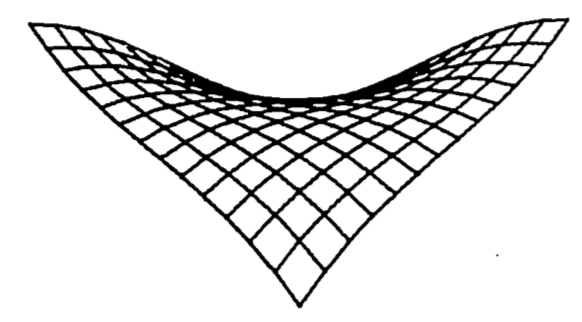
\includegraphics[width=0.4\linewidth]{figures/fig-calcdiff-11} \caption{Saddle point of a waterfall function.}\label{fig:fig-calcdiff-11}
\end{figure}

\hypertarget{bibliography}{%
\section{BIBLIOGRAPHY}\label{bibliography}}

\textbf{CALCULUS}

Ayres, F., Jr., 1964. Theory and Problems of Differential and Integral Calculus, second ed., Schaum's Outline Series, McGraw-Hill, New York.

Clow, D. J. and Urquhart, N. S., 1974. Mathematics in Biology, Norton, New York.

Keisler, H. J., 1971. Elementar Calculus: An A roach Usin: Infinitesimals, Prindle, Weber and Schmidt, Boston.

Sternberg, W., Walker, R. J. et al., 1968. Calculus, A Computer Oriented Presentation, The Center for Research in College Instruction in Science and Mathematics (CRICISAM), Florida State University, Tallahassee.

Thomas, G. B., Jr., 1968. Calculus and Analytic Geometry, fourth ed., Addison-Wesley, Reading, Massachusetts.

\textbf{TABLES}

Handbook of Mathematical Functions, 1964. Abramowitz, M. and I. Stegun, eds., National Bureau of Standards, Applied Mathematics Series, 55, Washington, D.C.

Handbook of Mathematical Tables, 1964. Weast, R. C., Selby, S. M. and C. D. Hodgman, eds., The Chemical Rubber Co., Cleveland. GENERAL

Alexander, R. M., 1968. Animal Mechanics, University of Washington Press, Seattle.

Bayne, B. L., Thompson, R. J. and J. Widdows, 1973. ``Some Effects of Temperature and Food on the Rate of Oxygen Consumption by Mytilus edulis L.,'' in Effects of Temperature on Ectothermic Organisms, Wieser, E., ed., Springer-Verlag, New York.

Caughley, G., 1970a. Ecology 51:53.

Caughley, G., 1970b. N.Z. J. Sci. 13:209.

de Vries, D. A., 1975. ``Heat Transfer in Soils,'' in Heat and Mass Transfer in the Biosphere, Part I, de Vries, D. A. and N. H. Afgan, eds., John Wiley and Sons, New York.

Goldberg, S., 1958. Difference Equations, Wiley, New York.

Long, C., 1976. MAA Monthly, 83:370.

Nay, R., 1978. ``Mathematical Aspects of the Dynamics of Animal Populations,'' in Studies in Mathematical Biology, Part II, S. Levin, ed., Math. Assn. of America.

Sladen,13. 1969. ``The Ecology of Animal Communities,'' in Biology of Populations, Sladen, B. and F. Bang, eds., Elsevier, New York.

\hypertarget{problem-set-1}{%
\section{PROBLEM SET}\label{problem-set-1}}

\begin{enumerate}
\def\labelenumi{\arabic{enumi}.}
\item
  \begin{enumerate}
  \def\labelenumii{\alph{enumii}.}
  \tightlist
  \item
    The logistic population growth function satisfies the differential equation
    \[\frac{dx}{dt}=Ax(N-x)\]
    where \(x=x(t)\) is the population size and \(N\) is the carrying capacity of the environment. Use this equation to show that the maximum growth rate (max \(dx/dt\)) occurs at the inflection point \(x=N/2\). Assume \(A\) is positive. (HINT: write the equation with \(v = dx/dt\), and set \(dv/dx = 0\)).
  \end{enumerate}
\end{enumerate}

~~b. The ``relative growth rate'' is defined by
\[R=\frac{1}{x}(\frac{dx}{dt})\]
where \(dx/dt\) is as given in part (a). Let \(x\) be given in ``numbers of animals'' and evaluate the units of \(R\). The logistic curve is often used to describe ``crowding effects'' including intraspecies competition. Use the equation of part (a) to determine the value of \(x\) which maximizes \(R\), and explain this result in terms of crowding.

\begin{enumerate}
\def\labelenumi{\arabic{enumi}.}
\setcounter{enumi}{1}
\tightlist
\item
  Leaves usually have small openings called stomata to allow passage of gases between their interior and exterior. Through them carbon dioxide passes in for capture by photosynthesis and the resulting oxygen passes out. Water vapor also escapes through the stomata, sometimes leading to dehydration. Thus plants have guard cells around the stomata to regulate their size. Action of the guard cells varies the shape of stomatal openings from a long narrow slit to nearly a circle. Throughout most of this variation the opening has approximately the shape of an ellipse with a constant length perimeter, typically about 35 \(\mu\).\\
  A good approximation to the perimeter of an ellipse is
  \[P=2\pi\sqrt{(a^2+b^2)/2}\]
  The area is given by
  \[A=\pi ab\]
  Set \(P=35\) and evaluate the area, \(A\), in terms of just the width, \(b\). Show that the area reaches a maximum when a=b, i.e., when the stomatal opening is a circle.
\end{enumerate}

\begin{figure}
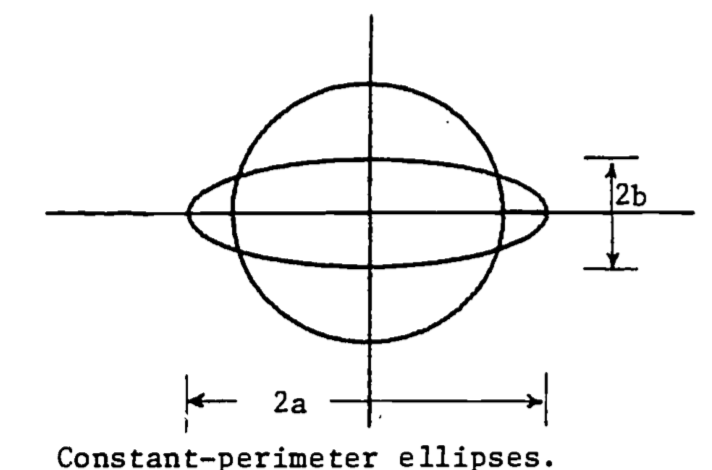
\includegraphics[width=0.75\linewidth]{figures/fig-calcdiff-p20} \caption{Constant-perimeter ellipses.}\label{fig:fig-calcdiff-p20}
\end{figure}

\begin{enumerate}
\def\labelenumi{\arabic{enumi}.}
\setcounter{enumi}{2}
\item
  In the O\textsubscript{2} consumption model represented by equation \eqref{eq:calcdiff-7}, the variable \(Q\) has units of \(\mu\)l/hr. Write \(Q\) in ml/hr and find \(\frac{\partial Q}{\partial m}\) for \(W\) = 1000 mg. What are the units of \(\frac{\partial Q}{\partial m}\)? What might this derivative represent biologically? That is, why would a biologist be interested in this derivative?
\item
  A study of shape changes in nemerteans and flatworms (Alexander, 1968) theorizes that a basement membrane encloses the body and contains fibers which run in helices around the body. From Figure b, if the length \(D\) of the fiber is fixed, then \(l = Dcos\theta\) and when the shape is cylindrical, the circumference and volume are \(2\pi r=Dsin\theta\), \(v=\pi r^2l\).
\end{enumerate}

\begin{figure}
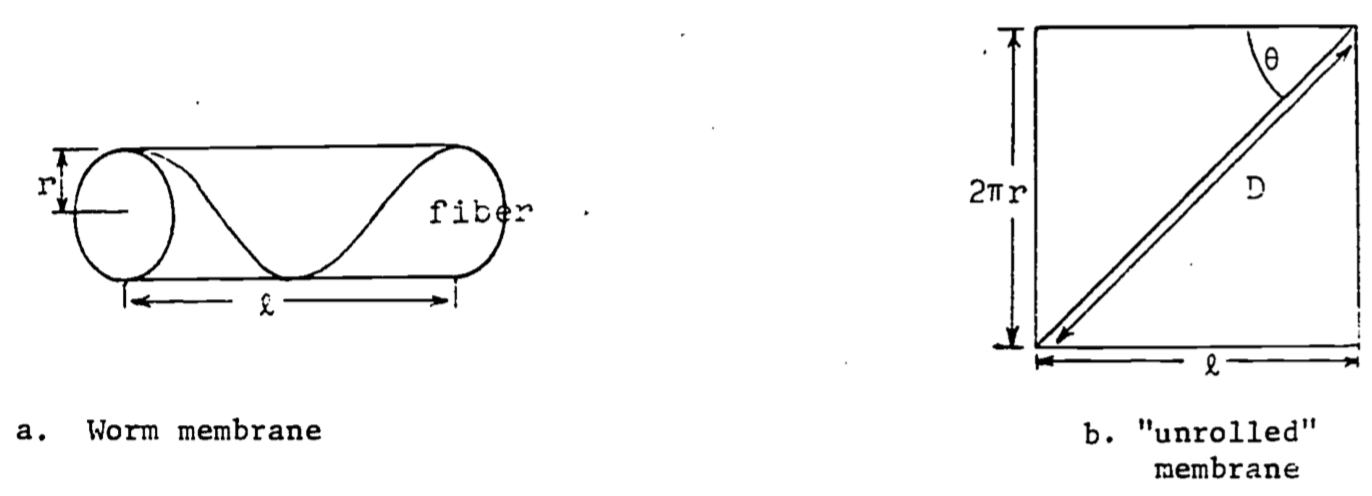
\includegraphics[width=0.75\linewidth]{figures/fig-calcdiff-p21} \end{figure}

~~a. Express \(v\) as a function of \(\theta\) (with \(D\) a parameter) and show \(v=0\) when \(\theta=0\) or \(\theta=\pi/2\) radians. What do these two cases mean physically?

~~b. Find \(\theta\) which gives a maximum for \(v\). Prove it is a relative maximum and not a relative minimum. Note that laboratory dissections show that in the relaxed worm the fibers run at about 55° to the axis of the body. Why would the relaxed worm have the maximum volume?

\begin{enumerate}
\def\labelenumi{\arabic{enumi}.}
\setcounter{enumi}{4}
\item
  Studies of insect flight (Alexander, 1968) use the theory of ``forced vibrations'' to explain the muscle action responding to nervous stimuli. If the ``forcing function'' is assumed to be
  \[Fsin(2\pi nt),\;\;\;\;t=\mbox{time},\;\;\;\;F=\mbox{constant},\]
  then the steady amplitude \(A\) (magnitude of the vibrations) is given by
  \[A=F[(s-4\pi^4n^2m)^2+(2\pi nK)^2]^{-1/2}\]
  where
  ~~~~\(K\) = viscous damping coefficient\\
  \hspace*{0.333em}\hspace*{0.333em}\hspace*{0.333em}\hspace*{0.333em}\(m\) = wing mass\\
  \hspace*{0.333em}\hspace*{0.333em}\hspace*{0.333em}\hspace*{0.333em}\(n\) = frequency\\
  \hspace*{0.333em}\hspace*{0.333em}\hspace*{0.333em}\hspace*{0.333em}\(s\) = stiffness of the vibrating medium\\
  Find the frequency \((n)\), called the \textbf{resonant} frequency, which gives the maximum amplitude.
\item
  This exercise verifies the location of the relative minimum in the example of ``water falling across a rock face''. The function is
  \[z=x^3+y^3-3xy+15\]
  Find all the critical points and determine which one is the relative minimum.
\item
  Heat transfer in soils depends on many factors; among them is the variation in the soil itself (de Vries, 1975).
\end{enumerate}

Since most of the variation is in the vertical direction, a simple mathematical model is the one dimensional diffusion equation,
\[C\frac{\partial T}{\partial t}=\frac{\partial}{\partial z}(\lambda\frac{\partial T}{\partial z})\]
where we define\\
\hspace*{0.333em}\hspace*{0.333em}\hspace*{0.333em}\hspace*{0.333em}\(T\) = temperature\\
\hspace*{0.333em}\hspace*{0.333em}\hspace*{0.333em}\hspace*{0.333em}\(t\) = time\\
\hspace*{0.333em}\hspace*{0.333em}\hspace*{0.333em}\hspace*{0.333em}\(z\) = vertical space coordinate\\
\hspace*{0.333em}\hspace*{0.333em}\hspace*{0.333em}\hspace*{0.333em}\(C\) = volumetric heat capacity\\
\hspace*{0.333em}\hspace*{0.333em}\hspace*{0.333em}\hspace*{0.333em}\(\lambda\) = thermal conductivity\\
When \(C\) and \(\lambda\) are uniform in depth and constant in time, we have the simple diffusion equation:
\[\frac{\partial T}{\partial t}=a\frac{\partial^2 T}{\partial z^2}\]
where \(a = \lambda/C\) is called the thermal diffusivity of the soil. The temperature As at the surface gives boundary conditions for the model. For sinusoidal variation of surface temperature, we can write the boundary conditions as
\[T(t,0)=T_a+\theta_0cos\omega t\]
\[T(t,\infty)=T_a=\mbox{constant}\]
Show that the solution to this model is given by the following function:
\[T(t,z)=T_a+\theta_0e^{-z/d}cos(\omega t-z/d)\]
with
\[d=(2a/\omega)^{1/2}\]
Be sure to verify that this function satisfies the diffusion equation \textbf{and} the boundary conditions.

\hypertarget{answers-to-the-problem-set-1}{%
\section{ANSWERS TO THE PROBLEM SET}\label{answers-to-the-problem-set-1}}

\begin{enumerate}
\def\labelenumi{\arabic{enumi}.}
\item
  \begin{enumerate}
  \def\labelenumii{\alph{enumii}.}
  \tightlist
  \item
    Find the \(x\) which gives max\((dx/dt)\). Differentiate \(dx/dt\) \textbf{with respect to \(x\)}, equate to zero and solve for \(x\):
    \[\frac{d}{dx}(\frac{dx}{dt})=A(N-2x)\]
    \[0=A(N-2x)\]
    \[x=N/2\]
    Since the second derivative is negative, i.e.
    \[\frac{d^2}{dx^2}(dx/dt)=-2A<0\]
    then at \(x=N/2\), \(dx/dt\) is maximal.
    ~~b. Find \(dR/dx\), set equal to zero, solve for \(x\):
    \[R=\frac{1}{x}[Ax(N-x)]=A(N-x)\]
  \end{enumerate}
\end{enumerate}

\[\frac{dR}{dx}=-A<0\]
So no relative max exists, and the maximum must be at the lower end of the domain of \(x\): since \(0\le x\le N\), then max \((R)\) occurs at \(x=0\). This model then implies that crowding effects are present whenever \textbf{any} animals exist.

\begin{enumerate}
\def\labelenumi{\arabic{enumi}.}
\setcounter{enumi}{1}
\item
  \[35=2\pi\sqrt{(a^2+b^2)/2}\]
  \[(\frac{35}{2\pi})^2=\frac{a^2+b^2}{2}\]
  \[a=(\frac{35^2}{2\pi^2}-b^2)^{1/2}\]
  The area \(A\) in terms of \(b\) is then
  \[A=\pi(\frac{35^2}{2\pi^2}-b^2)^{1/2}b=\pi(\frac{35^2b^2}{2\pi^2}-b^4)^{1/2}\]
  Maximize \(A(b)\):
  \begin{align*}
  \frac{dA}{db}&=\frac{\pi}{2}(\frac{35^2b^2}{2\pi^2}-b^4)^{-1/2}(\frac{35^2b}{\pi^2}-4b^3) \\
  0&=\frac{35^2b}{\pi^2}-4b^3,\;\;\;\;\mbox{assume }b\not=0 \\
  &=\frac{35^2}{\pi^2}-4b^2 \\
  b&=\frac{35}{2\pi},\;\;\;\;\mbox{since }b>0 \\
  a&=(\frac{35^2}{2\pi^2}-\frac{35^2}{4\pi^2})^{1/2}=\frac{35}{2\pi},\;\;\;\;\mbox{since }a>0
  \end{align*}
  Thus the maximum area occurs when \(a=b\), i.e.~a circle.
\item
  To convert \eqref{eq:calcdiff-7} so \(Q\) is in ml/hr, we divide by 1000:
  \[Q=1.87\times10^{-3}(m+1)W^{0.7}\]
  \begin{align*}
  \frac{\partial Q}{\partial m}&=1.87\times10^{-3}W^{0.7} \\
  &=0.234\;\;\;\;\mbox{for } W = 1000
  \end{align*}
  The units are then ml O\textsubscript{2} per hour per unit of activity.
\end{enumerate}

4.a. First solve for \(r(\theta)\):

\begin{align*}
&r=\frac{D}{2\pi}sin\theta \\
&v=(\frac{D}{2\pi}sin\theta)^2(Dcos\theta) \\
&v(\theta)=\frac{D^3}{4\pi}sin^2\theta cos\theta \\
&v(0) = 0\;\;\mbox{since}\;\;sin(0)=0 \\
&v(90^{\circ})= 0\;\;\mbox{since}\;\;cos(90^{\circ})=0
\end{align*}

~~b.

\begin{align*}
&\frac{dv}{d\theta}=\frac{D^3}{4\pi}\{2sin\theta cos^2\theta-sin^3\theta\} \\
&0=2sin\theta cos^2\theta-sin^3\theta\;\;\;\;\mbox{Assume }\;\theta > 0 \\
&0=2cos^2\theta - sin^2\theta \\
&sin^2\theta=2cos^2\theta \\
&tan\theta=\sqrt{2} \\
&\theta = 54.74^{\circ}
\end{align*}

\begin{enumerate}
\def\labelenumi{\arabic{enumi}.}
\setcounter{enumi}{4}
\tightlist
\item
  Maximize \(A\) by minimizing the denominator:
  \[0=\frac{d}{dn}[(s-4\pi^2n^2m)^2+(2\pi nK)^2]=2(s-4\pi^2n^2m)(-8\pi^2mn)+8\pi^2K^2n\]
  \[0=-2(ms-4\pi^2m^2n^2)+K^2\]
  \[2ms-K^2=8\pi^2m^2n^2\]
  \[n=\frac{2ms-K^2}{8\pi^2m^2}\]
\item
  First calculate the required partial derivatives:
  \[\frac{\partial z}{\partial x}=3x^2-3y,\;\;\;\;\frac{\partial z}{\partial y}=3y^2-3x\]
  \[\frac{\partial^2 z}{\partial x^2}=6x,\;\;\;\;\frac{\partial^2 z}{\partial x\partial y}=-3,\;\;\;\;\frac{\partial^2z}{\partial y^2}=6y\]
  Now find the critical point(s) by simultaneously solving
  \[\frac{\partial z}{\partial x}=0\;\;\;\mbox{and}\;\;\;\frac{\partial z}{\partial y}=0\]
\end{enumerate}

Thus
\[3x^2-3y=0\;\;\;\;3y^2-3x=0\]
From the first equation we obtain:
\[y=x^2\]
Substitute into the second equation and solve for \(x\):
\[3(x^2)^2-3x=0\]
\[3x(x^3-1)=0\]
Thus \(x=0,\;1\). The minimum is said to be at \((1,1)\).\\
With \(x=1\) we evaluate \(y\):
\[y=(1)^2=1\]
To classify this critical point, we evaluate
\[(\frac{\partial^2 z}{\partial x^2})(\frac{\partial^2z}{\partial y^2})-(\frac{\partial^2z}{\partial x\partial y})^2\;\;\;\mbox{at}\;\;\;(x,y)=(1,1)\]
\[(6\cdot1)(6\cdot1)-(-3)^2=36-9>0\]
Since
\[\frac{\partial^2 z}{\partial x^2}=6>0\;\;\;\mbox{at}\;\;\;(x,y)=(1,1)\]
then \((1,1)\) is indeed a relative minimum.

\begin{enumerate}
\def\labelenumi{\arabic{enumi}.}
\setcounter{enumi}{6}
\tightlist
\item
  First show the boundary conditions to be satisfied:
  \begin{align*}
  T(t,0)&=T_a+\theta_0e^{-0/d}cos(\omega t-0/d) \\
  &=T_a+\theta_0cos\omega t \\
  T(t,\infty)&=T_a+\theta_0e^{-\infty/d}cos(\omega t-\infty/d) \\
  &=T_a+0 \\
  &=T_a
  \end{align*}
  Now show that the diffusion equation is satisfied:
\end{enumerate}

\begin{align*}
\frac{\partial T}{\partial t}&=-\theta_0e^{-z/d}\omega sin(\omega t-z/d) \\
\frac{\partial T}{\partial z}&=-\frac{1}{d}\theta_0e^{-z/d}cos(\omega t-z/d)-\theta_0e^{-z/d}(-\frac{1}{d})sin(\omega t-z/d) \\
&=\frac{\theta_0e^{-z/d}}{d}[sin(\omega t-z/d)-cos(\omega t-z/d)] \\
\frac{\partial^2 T}{\partial z^2}&=(-\frac{1}{d})\frac{\theta_0}{d}e^{-z/d}[sin(\omega t-z/d)-cos(\omega t-z/d)] \\
&-(\frac{1}{d})\frac{\theta_0}{d}e^{-z/d}[cos(\omega t-z/d)+sin(\omega t-z/d)] \\
&=-\frac{2\theta_0}{d^2}e^{-z/d}sin(\omega t-z/d)
\end{align*}
Substituting into the diffusion equation:
\[-\theta_0e^{-z/d}\omega sin(\omega t-z/d)=-a\frac{2\theta_0}{d^2}e^{-z/d}sin({\omega t-z/d})\]
The equation is certainly true when \(sin(\omega t-z/d)=0\). Now assume that \(sin(\omega t-z/d)\not=0\) and divide both sides by \(-\theta_0e^{-z/d}sin(\omega t-z/d\):
\[\omega = 2a/d^2\]
Substituting for \(d\), we obtain
\[\omega = 2a/[(2a/\omega)^{1/2}]^2=\omega\]
Thus the equation is indeed satisfied.

\hypertarget{additional-problems-1}{%
\section{ADDITIONAL PROBLEMS}\label{additional-problems-1}}

\begin{enumerate}
\def\labelenumi{\arabic{enumi}.}
\tightlist
\item
  In the example in the text treating oxygen consumption(see also problem 3 above), the oxygen consumption \((Q)\) depended on both the activity level \((m)\) and the dry weight \((W)\):
  \[Q=0.00187(m+1)W^{0.7}\]
  where the units of \(Q\) are mlO\textsubscript{2}/hr. For this exercise, we use the correspondence
  \[Q \rightarrow z,\;m \rightarrow x,\;W\rightarrow y\]
  so that the equation is
  \[z=0.00187(x+1)y^{0.7}\]
\end{enumerate}

\begin{enumerate}
\def\labelenumi{\alph{enumi}.}
\item
  Evaluate the first partial derivative \(\partial z/\partial x\). If you plot \(\partial z/\partial x\) with increasing \(x\), is it supposed to be a straight line, concave upward, concave downward?
\item
  Now reverse the roles of \(x\), \(y\): evaluate \(\partial z/\partial y\).If you were to plot \(\partial z/\partial y\) against \(x\), is the shape supposed to be a straight line, circle, parabola \ldots{} ?
\end{enumerate}

\begin{enumerate}
\def\labelenumi{\arabic{enumi}.}
\setcounter{enumi}{1}
\item
  This exercise illustrates how different parameter values can affect the properties of a function and its critical points. Function 2 is used in this exercise and is a simple polynomial in two independent variables:
  \[z=(P1)x^2+(P2)y^2\]
  Calculate all the partial derivatives needed to locate and classify a critical point. Set values for \(P1\), \(P2\) and evaluate the critical point.
\item
  When a beam of rectangular cross-section is cut lengthwise from a log, its strength can sometimes be well described by the following function:
  \[S=kWD^2\]
  where\\
  \hspace*{0.333em}\hspace*{0.333em}\hspace*{0.333em}\hspace*{0.333em}\hspace*{0.333em}\hspace*{0.333em}\(S\) = strength of beam\\
  \hspace*{0.333em}\hspace*{0.333em}\hspace*{0.333em}\hspace*{0.333em}\hspace*{0.333em}\hspace*{0.333em}\(W\) = width of beam\\
  \hspace*{0.333em}\hspace*{0.333em}\hspace*{0.333em}\hspace*{0.333em}\hspace*{0.333em}\hspace*{0.333em}\(D\) = depth of beam\\
  as shown in Figure \ref{fig:fig-calcdiff-A}, and where \(k\) is a constant which depends on the type of tree used. Assume that the log is circular in cross-section and that the beam is cut so each corner reaches the outside of the log, as shown. Assume \(k\) = 0.1. Find the width and depth of the beam which give the maximum strength. Assume the radius of the log is \(r\).
\end{enumerate}

\begin{figure}
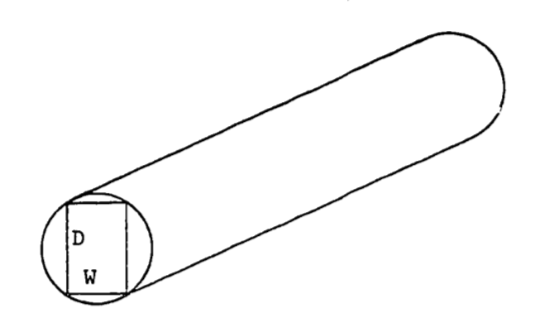
\includegraphics[width=0.75\linewidth]{figures/fig-calcdiff-A} \caption{Rectangular beam cut from a log.}\label{fig:fig-calcdiff-A}
\end{figure}

\begin{enumerate}
\def\labelenumi{\arabic{enumi}.}
\setcounter{enumi}{3}
\tightlist
\item
  Animal populations newly introduced into a region have been observed to increase rapidly in number and soon thereafter to fall drastically (Caughley 1970a, b) as indicated in Figure \ref{fig:fig-calcdiff-B}. One theory is that the population at first ``senses'' an infinite food supply and then reproduces rapidly to the point of overgrazing the area. The birth rate remains the same but the death rate (perhaps of young) dramatically increases until the population is low enough to match the food supply. The population then increases more slowly and seems to stabilize. Migration is also involved but is poorly understood. The second population rise to a ``steady-state'' suggests some adaptation or social ``learning'' by the population concerning their new environment.
\end{enumerate}

\begin{figure}
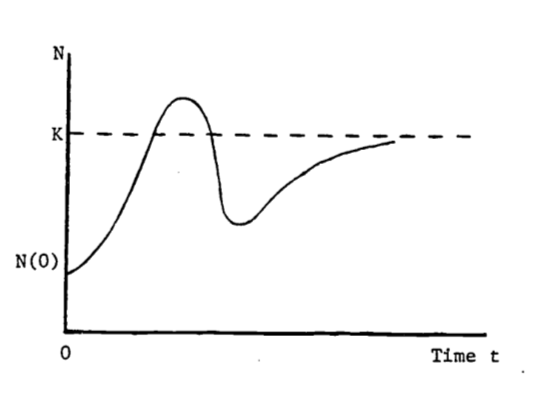
\includegraphics[width=0.75\linewidth]{figures/fig-calcdiff-B} \caption{Population dynamics of introduced species.}\label{fig:fig-calcdiff-B}
\end{figure}

\begin{enumerate}
\def\labelenumi{\alph{enumi}.}
\item
  Consider the logistic equation written as follows:
  \[N(t)=K(1+be^{-rt})^{-1}\]
  where \(K\), \(b\), \(r\) are positive constants, and \(N(0) < K\). In an attempt to describe the behavior in Figure B, one could modify the above logistic function by allowing \(r\) to vary over time, i.e.~\(r = r(t)\). Can the population ever exceed \(K\)? If not, then this modified logistic function is not a good model. Answer this for a general \(r(t)\) in any fashion: by examining the function \(N(t)\) itself, by evaluating the maximum of \(N(t)\), etc.
\item
  An alternate model is developed if the discreteness of the population is taken into account. The logistic function in part (a) assumes that the population size, \(N(t)\), will change \textbf{continuously} as time changes. In certain species, populations do not change size smoothly (see Sladen and Bang 1969). The breeding time is a short period, once a year so that many off-spring are born at the same time. The population size then increases in large jumps. This discrete change is not modeled well by differential equations. A closely related field is the study of ``difference equations'' (see Goldberg 1958) where discrete changes are allowed. The derivative of the logistic function satisfies the differential equation
  \[\frac{dN(t)}{dt}=rN(t)\Big(\frac{K-N(t)}{K}\Big)\]
  From this formulation, we see that the logistic model assumes that the population is always aware of how far from the carrying capacity is the current population size and so continuously adjusts for this difference. (Note that the derivative depends on this difference, \(K-N(t)\)). Actually, plentiful food one season may cause too many births the following season, with a definite time lag between abundant food and severe overpopulation and with few adjustments in between.
\end{enumerate}

The computer is used here to illustrate this inadequacy of differential calculus. The derivative above is replaced by a difference:
\[\frac{N(t+1)-N(t)}{(t+1)-t}=rN(t)\Big(\frac{K-N(t)}{K}\Big)\]
This model assumes the population changes only once per time period (e.g.~annually) and is unable to adjust in between. Is this more or less realistic than the original logistic model? How would you include social or genetic ``learning'' into the model? That is, once the population size rises and then falls, what parameters might change in the model so that the next rise would be more gradual?

\begin{enumerate}
\def\labelenumi{\arabic{enumi}.}
\setcounter{enumi}{4}
\tightlist
\item
  The reaction \((Y)\) of the body to a dose \((X)\) of drug can be represented by the function:
  \begin{align*}
  Y(X)&=X^2(P1/2-P2\cdot X/3) \\
  &=\frac{P1}{2}X^2-\frac{P2}{3}X^3 \\
  \end{align*}
\end{enumerate}

where \(P1\) and \(P2\) depend on certain body characteristics and on the maximum dosage which can be administered. \(Y\) indicates the strength of the reaction, measured in millimeters of mercury if blood pressure is being tested, or perhaps degrees Celsius if change in body temperature is being measured.

Find the dose that has ``maximum sensitivity,'' i.e.~where the \textbf{rate of increase} of \(Y\) is greatest. Is this ``critical point'' a maximum or minimum for \(Y\)"? What is this point called on the graph for \(Y\)?

\hypertarget{answers-to-the-additional-problems}{%
\section{ANSWERS TO THE ADDITIONAL PROBLEMS}\label{answers-to-the-additional-problems}}

\begin{enumerate}
\def\labelenumi{\arabic{enumi}.}
\item
  \(\partial z/\partial x=(0.00187y^{0.7})=\)constant for given \(y\).\\
  Exposed profile should be a straight line.\\
  \(\partial z/\partial y=(0.00187)(x+1)(0.7)y^{-0.3}\)\\
  Exposed profile curves upward with decreasing slope.
\item
  \(\partial z/\partial x=2(P1)x\), \(\partial z/\partial y=2(P2)y\)\\
  \(\partial^2 z/\partial x^2=2(P1)\), \(\partial^2z/\partial x\partial y=0\), \(\partial^2z/\partial y^2=2(P2)\)\\
  \(\partial z/\partial x=0\) if \(x=0\)\\
  \(\partial z/\partial y=0\) if \(y=0\)\\
  Thus \((x,y)=(0,0)\) is the only critical point.\\
  To classify the critical point, evaluate:
  \[\frac{\partial^2z}{\partial x^2}\frac{\partial^2z}{\partial y^2}-\Big(\frac{\partial^2 z}{\partial x\partial y}\Big)^2=4(P1)(P2)\]
  Pick \(P1=.6\), \(P2=1.0\)\\
  Then \(4(P1)(P2)>0\), \(\frac{\partial^2z}{\partial x^2}=2(P1)>0\) and the point is a relative minimum.
\item
  We use the Pythagorean theorem to obtain
\end{enumerate}

\[(2r)^2=W^2+D^2\]
Thus
\begin{align*}
D^2&=4r^2-W^2 \\
S&=(0.1)4r^2W-(0.1)W^3 \\
\frac{dS}{dW}&=(0.4)r^2-(0.3)W^2 \\
0&=(0.4)r^2-(0.3)W^2
\end{align*}

The critical point is then at \(W=\sqrt{4r^2/3}=2r/\sqrt{3}\)
We have
\[\frac{d^2S}{dW^2}=-0.6W<0\]
so that when \(W=2r/\sqrt{3}\), \(S\) is indeed at a maximum.\\
The depth is then
\begin{align*}
D&=\sqrt{4r^2-W^2} \\
&=\sqrt{4r^2-4r^2/3} \\
&=2\sqrt{2/3}r
\end{align*}

4.a. Even assuming \(r = r(t)\), N cannot exceed \(K\) if \(N(0) < K\). We see this by writing \(N\) as a fraction.
\[N(t)=\frac{K}{1+be^{-r(t)t}}\]
b. Treat \(r(t)\) in the difference equation model, with
\begin{align*}
r(0)&=r_0 \\
r(1)&=r_0/2 \\
r(2)&=r_0/3 \\
r(3)&=r(2)
\end{align*}
or some such scheme to decrease r as time increases.

\begin{enumerate}
\def\labelenumi{\arabic{enumi}.}
\setcounter{enumi}{4}
\tightlist
\item
  Evaluate the derivative.
  \[Y'=(P1)X-(P2)X^2\]
  The ``rate of increase'' of \(Y\) is greatest when \(Y'\) is maximal. Find, the max(\(Y'\)) by differentiating \(Y'\) and setting \(Y'' = 0\).
  \begin{align*}
  Y''&=\frac{d(Y')}{dx}=(P1)-(2)(P2)X \\
  0&=(P1)-(2)(P2)X \\
  X&=(P1)/(2(P2))
  \end{align*}
  The value for \(Y\) is then
  \[Y=\Big[\frac{P1}{2(P2)}\Big]^2\Big[\frac{P1}{2}-\frac{(P1)(P2)}{6(P2)}\Big]=\frac{(P1)^3}{12(P2)^2}\]
  This point is an inflection point on the graph \(Y\) versus \(X\).
\end{enumerate}

\hypertarget{dimmethods}{%
\chapter{Dimensional Methods.}\label{dimmethods}}

author: Fletcher, R. I.

\hypertarget{preface-2}{%
\section{PREFACE}\label{preface-2}}

This module is concerned with the conventional techniques such as concepts of measurement, fundamental and derived units, checking equations for dimensional consistency, and the metric system. Attention is directed almost exclusively to the dimensional necessities of scientific statements, and only incidentally to their scientific sufficiencies. The International System of Units, SI, is discussed and a problem set is used to provide practice with the metric system. The concept of dimensional homogeneity,i.e., that all terms of an equation must consist of like dimensions raised to like powers, is analyzed, and a related problem set is provided. Concepts presented in the module require knowledge of basic algebra.

\hypertarget{introduction.}{%
\section{INTRODUCTION.}\label{introduction.}}

The common objective in scientific research, whatever our particular field of interest, is to discover those exact relationships that exist among the measurable quantities of nature. And typically, when our perceptions of those relationships are confirmed by experiment to have sufficient generality, we look upon our perceptions as natural laws. Although we often accept apparent truths about the natural universe that are difficult to quantify (Darwin's thesis of evolution, for example), the absolutely necessary condition for ``exactness'' in a scientific law is that its formulation consist of measurable quantities whose definitions depend, in turn, entirely upon a set of dimensions. In this formal sense, such classical sciences as physics and chemistry--as well as much of modern biology--are said to be exact, but obviously, some topics of natural science (such as Darwin's thesis of evolution) are characteristically inexact.

Dimensional formalities do not, of course, insure scientific infallibility, and we sometimes originate dimensionally perfect formulae that turn out to be irrelevant, inaccurate, or erroneous, but dimensional completeness fulfills the necessary condition for exactness in a scientific statement and we cannot proceed to the more practical concerns of scientific sufficiency until we satisfy in our formulae the formalistic requirements of dimensional exactitude--otherwise our formulae are meaningless. We shall, in fact, be concerned here almost exclusively with the dimensional necessities of scientific statements and only incidentally with their sufficiencies. Unlike the self-consistent arguments of purely mathematical demonstrations, scientific sufficiency rests instead with empirical evidence. Although dimensional methods provide us with the means for determining the obligatory (the formally necessary) relationships among the quantities of a scientific formula, we should clearly understand that experimentation, observation, and insight really determine just which quantities go into the formula in the first place.

So as to distinguish between differing \emph{magnitudes} of a particular dimension, we must have access to a \emph{scale} (or \emph{unit}) of comparison. In saying ``the height of that tree is nine meters'' we imply that we have chosen \emph{length} as the dimension of definition and the \emph{meter} as the corresponding scale unit of comparison. In making the observation let us also note that ``length'' might have defined our concept of tallness but not necessarily our whole notion of the tree itself. This is not a trivial acknowledgement; it points up the fact that scientific definitions describe \emph{attributes} of natural entities or occurrences, not their ontological meanings or their elemental reasons for existence. While we might employ the universal law of gravitation, let us say, to quantify the attribute of attraction between bodies of mass, the law of gravitation consists wholly of dimensional relationships and tells us nothing of the ``essence'' of gravity, nor why every corporeal body in the universe should have a gravitational field in the first place. Although we may share an intense curiosity about such questions, their resolutions are usually reserved to inquiries external to science proper. Should perplexity exist over the \emph{scientific} description of some natural quantity, its origin should be sought not in some mysterious, hidden characteristic of the natural quantity, but rather in the ambiguity of the quantity's dimensional definition.

In view of these definitional objectives, we must accord to every kind of natural quantity its defining dimension, but these defining dimensions need not be wholly independent of one another. Since we desire that differing natural quantities be related through natural laws, then for simplicity and clarity of definition we should keep the number of \emph{independent} dimensions to a minimum. This minimum set of independent dimensions we shall call \emph{fundamental}, and all other dimensions derived from the fundamental set we shall call \emph{derived}. Similarly, the magnitudes (the scale units) corresponding to the fundamental dimensions are viewed as fundamental magnitudes, and those corresponding to the derived dimensions as derived magnitudes. An obvious example of a derived quantity would be that of velocity--the velocity, say, of an aircraft whose pilot reads derived units of velocity magnitude directly from the scale of his airspeed indicator. Irrespective of the particular scale system on the airspeed indicator, we perceive the velocity \emph{dimension} to be derived, in general, from the more fundamental set of dimensions, length and time, and with corresponding symbols \(V\), \(L\) ,\(T\) we can write that general dimensional relationship as

\[[V] \equiv [LT^{-1}]\]

read as ``the dimension \(V\) is defined as the ratio of dimensions \(L\) and \(T\).'' The particular scale measurement of, say, 500 kilometers per hour would correspond to 500 derived units of velocity magnitudes derived from the kilometer and the hour. We would write the scale relationship for this particular example as

\[v = 500 km\cdot hr^{-1}\]

with an obvious correspondence between fundamental unit magnitudes ``km'' and ``hr'' and the fundamental dimensions \(L\) and \(T\). The unit symbol ``km\(\cdot\)hr\textsuperscript{-1}'' is as much a part of the value of quantity \(v\) as is the numerical value ``500''. The conventions (the symbolic styles) employed in this example suggest the convenient fact that we can manipulate dimensional and scale symbols as algebraic entities.

There is a certain arbitrariness of choice in the number and nature of the ``fundamental'' dimensions, whether we are thinking of our needs in choosing dimensions for actual measurement purposes or for the more formalistic requirements of theoretical models (and there is also considerable latitude in the selection of the scale units we might regard as fundamental; those suited for one problem may not be suited for another). Because of the strong historical precedent of Newtonian mechanics, the three natural concepts of space, time, and mass are often regarded as being fundamental in the absolute sense, but, in fact, more than three fundamental dimensions are sometimes desirable, and we shall see that differing sets of fundamental dimensions can be selected, none of which need be regarded as absolutely fundamental.

\hypertarget{problem-set-1.}{%
\subsection{PROBLEM SET 1.}\label{problem-set-1.}}

\begin{enumerate}
\def\labelenumi{\arabic{enumi}.}
\item
  Employ the dimensional set \(M\) (mass), \(V\) (velocity), \(T\) (time), and do the following exercise. The attached solutions may be consulted if necessary.

  \begin{enumerate}
  \def\labelenumii{(\alph{enumii})}
  \tightlist
  \item
    The linear acceleration of a particle can be envisioned as the increase or decrease in the velocity of the particle, measured over a short time period. Write the dimensions of linear acceleration.\\
  \item
    The magnitude of force on a body wholly free to move can be calculated as the product of the body's mass and its linear acceleration. Write the dimensions of mechanical force.\\
  \item
    The instantaneous kinetic energy of a moving body is proportional to the mass of the body and to the square of its linear speed. Write the dimensional formula for kinetic energy.
  \end{enumerate}
\item
  Employ the dimensional set \(M\) (mass), \(L\) (length), \(T\) (time), and do (a), (b), (c) of Exercise 1.
\item
  Employ the dimensional set \(F\) (force), \(L\) (length), \(T\) (time), and do the following exercise.

  \begin{enumerate}
  \def\labelenumii{(\alph{enumii})}
  \tightlist
  \item
    Problem (c) of Exercise 1.\\
  \item
    The work done in moving the body of Problem 1(c) is equivalent to the product of the force acting on the body and the distance the body moves while the force is being applied. Write the dimensional formula for mechanical work.\\
  \item
    Power is defined as the time rate of energy expenditure (or, equivalently, as the rate at which work is done). Write the dimensional formula for the power of the agency that imparts the motion to the body of Problem 3(b).
  \end{enumerate}
\item
  Employ the dimensional set \(M\), \(L\), \(T\) and do (b), (c) of Exercise 3.
\item
  In the mks system of measurement, the meter (m) is the unit standard of length, the kilogram (kg) the unit standard of mass, and the second (sec) the unit standard of time. The derived unit of force in the mks system is called the ``newton'' (nt), the derived unit of energy is called the ``joule'', and the derived unit of power is called the ``watt''. Employ the mks system of measurement and write the unit magnitudes of the corresponding quantities described in Exercises 2, 3, 4.
\end{enumerate}

\hypertarget{si-units.}{%
\section{SI UNITS.}\label{si-units.}}

In the making of scientific syntheses, our mutual needs for clear thinking and precision of meaning--as well as the need for clarity in communications between us have an obvious dependence on the exactness of our reference standards and the precision we choose to employ in the characterizing of those natural quantities that ultimately enter our formulations as symbols. Our usages here shall conform, with little revision, to the conventions and standards known as the International System of Units (abbreviated SI for \emph{Systeme International}), supplemented where necessary by the practices of the National Bureau of Standards (NBS). In the SI system, the fundamental metric units associated with dimensions \(M\), \(L\), \(T\) are the kilogram, the meter, and the second (customarily called the ``mks system''). A variety of auxiliary metric units are employed in practice (such as the kilometer, the angstrom, the gamma, and so on), but the auxiliary or supplementary set of metric units most commonly associated with dimensions \(M\), \(L\), \(T\) are the gram, the centimeter, and the second (customarily called the ``cgs system'').

The following definitions for mechanical quantities have been abstracted from publications of NBS (1964,1968) and Cray (1972). For comprehensive tabulations of the quantities appropriate to optics, acoustics, and electricity, see the \emph{Handbook of the American Institute of Physics}, the \emph{Handbook of Chemistry and Physics} (Chemical Rubber Co.), or the
\emph{Handbook of the National Bureau of Standards}, which is edited and published annually.

\hypertarget{fundamental-mechanical-units}{%
\subsection{FUNDAMENTAL MECHANICAL UNITS}\label{fundamental-mechanical-units}}

\emph{Meter}. Unit of length mks system. Symbol m, dimension L. By international agreement (1960) defined to be 1,650,763.73 wavelengths of the orange-red line of krypton 86, which replaces the length standard based on the platinum-iridium meter bar in Paris.

\emph{Kilogram}. Unit of mass mks system. Symbol kg, dimension M. Defined to be the mass of a certain cylinder of platinum-iridium alloy, called the International Prototype Kilogram, preserved at the International Bureau of Weights and Measures in Paris.

\emph{Second}. Unit of time mks system. Symbol sec, dimension T. By international agreement (1960) defined to be 1/31,556,925.9747 of the tropical year 1900. (A ``tropical year'' is the interval of time between two successive passages of the sun through the vernal equinox.) A more recent international conference adopted provisionally a new definition of the second as the time corresponding to 9,192,631,770 oscillations of the cesium atom in the so-called atomic clock.

\hypertarget{temperature-scales}{%
\subsection{TEMPERATURE SCALES}\label{temperature-scales}}

In 1968 the International Committee on Weights and Measures officially adopted the ``International Practical Temperature Scale'', which is based on the concept of temperature (variable symbol 0, dimension 0) as being that of thermodynamic temperature. The unit magnitude of the International Scale is the degree Kelvin (symbol K). The degree Kelvin is the fraction 1/273.16 of the triple point of water. The Celsius temperature scale is defined in terms of the Kelvin scale as
\[\theta_c=\frac{1^{\circ}C}{1K}\Big(\theta_k-\theta_0\Big)\]
where \(\theta_c\) is the temperature magnitude on the Celsius scale, \(\theta_k\) the temperature magnitude on the Kelvin scale, and \(\theta_0\) = 273.15K (the ice point of water). The scale unit of the Celsius temperature is the degree Celsius (symbol \(^{\circ}\)C), equal in magnitude to the degree Kelvin. Reference point relationships between Kelvin, Celsius, and Fahrenheit scales are:

\begin{itemize}
\tightlist
\item
  0K = -273.15 \(^{\circ}\)C = -459.67\(^{\circ}\)F (``absolute'' zero),\\
\item
  273.15K = 0\(^{\circ}\)C = 32\(^{\circ}\)F (the ice point),\\
\item
  273.16K = 0.01\(^{\circ}\)C = 32.018\(^{\circ}\)F (equilibrium between solid, liquid, and vapor phases of water; the triple point),\\
\item
  373.15K = 100\(^{\circ}\)C = 212\(^{\circ}\)F (the boiling point of water).
\end{itemize}

The relationships between the Kelvin, Celsius, and Fahrenheit scales are linear and appear as straight lines when graphed.

\hypertarget{supplementary-mechanical-units-cgs-and-english-systems}{%
\subsection{SUPPLEMENTARY MECHANICAL UNITS (cgs and English systems)}\label{supplementary-mechanical-units-cgs-and-english-systems}}

\emph{Centimeter}. Unit of length cgs system. Symbol cm, dimension L. Defined to be 1/100 meter.

\emph{Gram}. Unit of mass cgs system. Symbol g, dimension M. Defined to be 1/1000 kilogram.

\emph{International Yard}. Unit of length. Symbol yd, dimension L. Defined by agreement between the United States and the British Commonwealth (1959) to be 0.9144 meter.

\emph{International Pound}. Unit of mass. Symbol lb, dimension M. Defined by agreement between the United States and the British Commonwealth (1959) to be 0.45359237 kilogram.

\emph{Angstrom}. Unit of length. Symbol \(\mathring{A}\), dimension L. Defined to be 10\(^{-8}\) cm. Gamma. See microgram.

\emph{Microgram}. Unit of mass. Symbol \(\mu\)g, dimension M. Defined to be 10\(^{-6}\) g.

\emph{Micrometer}. Unit of length. Symbol \(\mu\)m, dimension L. Defined to be 10\(^{-6}\) m (1/1000 cm). Equivalent to, but replaces, micron (symbol \(\mu\)).

\emph{Micron}. See micrometer.

\hypertarget{angular-units}{%
\subsection{ANGULAR UNITS}\label{angular-units}}

\emph{Degree}. Unit of angular measure. Symbol deg or \(^{\circ}\) (superscript), dimensionless, Defined as the angle subtended at the center by a circular arc 1/360 the circumference.

\emph{Radian}. Unit of angular measure. Symbol radian, dimensionless. Defined as the angle subtended at the center by a circular arc equal in length to the radius of the circle. 1 radian = 360/2\(\pi\) degrees angular measure.

\hypertarget{derived-units}{%
\subsection{DERIVED UNITS}\label{derived-units}}

\emph{Atmosphere}. Unit of pressure. Symbol atm, dimension FL\(^{-2}\) or ML\(^{-1}\)T\(^{-2}\). Defined to be the pressure exerted by dry atmosphere, 0\(^{\circ}\)C, at mean sea level. Equivalent to \(1.013250 \times 10^6 dyn\cdot cm^{-2}\) in cgs units.

\emph{Bar}. Unit of pressure. Symbol bar, dimension FL\(^{-2}\) or ML\(^{-1}\)T\(^{-2}\). Equal to \(10^5 nt\cdot m^{-2}\) in mks units.

\emph{British Thermal Unit (Mean)}. Unit of energy or quantity of heat. Symbol Btu, mechanical dimension ML\(^2\)T\(^{-2}\), thermal dimension H. Originally defined to be the quantity of heat energy required to raise the temperature of 1 lb mass of water 1\(^{\circ}\)F (averaged from 32\(^{\circ}\)F to 212\(^{\circ}\)F). Equivalent to 252.16038 gram calories.

\emph{Calorie (Mean)}. Unit of energy or quantity of heat. Symbol cal, mechanical dimension ML\(^2\)T\(^{-2}\), thermal dimension H. Originally defined to be the quantity of heat energy required to raise the temperature of 1 g mass of water 1\(^{\circ}\)C (averaged from 0\(^{\circ}\)C to 100\(^{\circ}\)C). Equivalent to 4.1840 joules.

\emph{Dyne}. Unit of force cgs system. Symbol dyn, dimension F or MLT\(^{-2}\), unit g\(\cdot\)cm\(\cdot\)sec\(^{-2}\). Force required to give 1 g mass an acceleration of 1 cm\(\cdot\)sec\(^{-2}\).

\emph{Erg}. Unit of work or energy cgs system. Symbol erg, dimension FL or ML\(^2\)T\(^{-2}\), unit dyn\(\cdot\)cm or g\(\cdot\)cm\(^2\cdot\)sec\(^{-2}\). Work done by a force of 1 dyne acting through a distance of 1 cm (10\(^7\) erg = 1 J).

\emph{Hertz}. Unit of frequency. Symbol Hz, dimension T\(^{-1}\), unit sec\(^{-1}\). Equivalent to, but replaces, unit cps (cycle per second).

\emph{Joule}. Unit of work or energy mks system. Symbol J, dimension FL or ML\(^2\)T\(^{-2}\), unit ntm or kg\(\cdot\)m\(^2\cdot\)sec\(^{-2}\). The work done by a force of 1 newton acting through a distance of 1 meter.

\emph{Liter}. Unit of volume (liquids and gases). Symbol 1, dimension L\(^3\). Originally defined to be the volume of 1 kg airfree \(H_2O\) at 4\(^{\circ}\)C (the maximum density temperature of water). Redefined by international agreement (1964) to be 1/1000 cubic meter (10\(^{-3}\)m\(^3\)) exactly.

\emph{Newton}. Unit of force mks system. Symbol N (alternate symbol nt), dimension F or MLT\(^{-2}\). Force required to give 1 kg mass an acceleration of 1 m\(\cdot\)sec\(^{-2}\).

\emph{Poise}. Unit of viscosity cgs system. Symbol P, dimension FL\(^{-2}\)T or ML\(^{-1}\)T\(^{-1}\), unit dyn\(\cdot\)cm\(^{-2}\cdot\)sec or g\(\cdot\)cm\(^{-1}\cdot\)sec\(^{-1}\). Shear viscosity, or resistance to flow, is defined as the ratio of shearing stress (tangential force per unit area) in a moving fluid and its associated rate of area deformation (\(dA/Adt\)). Shear viscosity is sometimes called the dynamic viscosity.

\emph{Poundal}. Unit of force. Symbol lbf (pound force), dimension F or MLT\(^{-2}\). Force required to give 1 lb mass an acceleration of 1 ft\(\cdot\)sec\(^{-2}\).

\emph{Stokes}. Unit of kinematic viscosity cgs system. Symbol St, dimension L\(^2\)T\(^{-1}\), unit cm\(^2\cdot\)sec\(^{-1}\). Kinematic viscosity in units of Stokes is defined to be the ratio of the dynamic viscosity (in poise) of a fluid to its cgs density (g\(\cdot\)cm\(^{-3}\)).

\emph{Torr}. Unit of pressure. Symbol torr, dimension FL\(^{-2}\) or ML\(^{-1}\)T\(^{-2}\). The pressure exerted by a column of mercury 1 mm in height, 0\(^{\circ}\)C. Equivalent to 13.3322 dyn\(\cdot\)cm\(^{-2}\) in cgs units.

\emph{Watt}. Unit of power or rate of work mks system. Symbol W, dimension FLT\(^{-1}\) or ML\(^2\)T\(^{-3}\), unit J\(\cdot\)sec\(^{-1}\) or nt\(\cdot\)m\(\cdot\)sec\(^{-1}\) or kg\(\cdot\)m\(^2\cdot\)sec\(^{-3}\). Work done or energy expended at the rate of l J\(\cdot\)sec\(^{-1}\).

An appendix summarizing the SI units and dimensions is attached.

\hypertarget{auxiliary-prefixes-of-the-metric-system-to-indicate-decimal-multiples-and-submultiples}{%
\subsection{AUXILIARY PREFIXES OF THE METRIC SYSTEM TO INDICATE DECIMAL MULTIPLES AND SUBMULTIPLES}\label{auxiliary-prefixes-of-the-metric-system-to-indicate-decimal-multiples-and-submultiples}}

\begin{longtable}[]{@{}cc@{}}
\toprule
Multiples and sub-multiples & Prefix\tabularnewline
\midrule
\endhead
10\textsuperscript{-18} & atto\tabularnewline
10\textsuperscript{-15} & femto\tabularnewline
10\textsuperscript{-12} & pico\tabularnewline
10\textsuperscript{-9} & nano\tabularnewline
10\textsuperscript{-6} & micro\tabularnewline
10\textsuperscript{-3} & milli\tabularnewline
10\textsuperscript{-2} & centi\tabularnewline
10\textsuperscript{-1} & deci\tabularnewline
10 & deka\tabularnewline
10\textsuperscript{2} & hecto\tabularnewline
10\textsuperscript{3} & kilo\tabularnewline
10\textsuperscript{6} & mega\tabularnewline
10\textsuperscript{9} & giga\tabularnewline
10\textsuperscript{12} & tera\tabularnewline
\bottomrule
\end{longtable}

\hypertarget{problem-set-2}{%
\subsection{PROBLEM SET 2}\label{problem-set-2}}

\begin{enumerate}
\def\labelenumi{\arabic{enumi}.}
\item
  Determine the number of 24-hour days in the tropical year 1900.
\item
  Write algebraic formulae for the relationships between

  \begin{enumerate}
  \def\labelenumii{(\alph{enumii})}
  \tightlist
  \item
    Kelvin and Fahrenheit temperature,\\
  \item
    Celsius and Fahrenheit temperature.
  \end{enumerate}
\item
  A molecule of water occupies a square cross-sectional area of about 10 \(\mathring{A}^2\). How many water molecules are needed to cover a square centimeter of surface?
\item
  Determine the kinetic energy in ergs of a molecule having a mass of \(2.0\times10^{-22}\)g and a velocity of \(4.0\times10^4\)cm\(\cdot\)sec\textsuperscript{-1}.
\item
  A red blood cell has a diameter of 7.5 microns; express its diameter in units of centimeter length.
\item
  Write as ordinary magnitudes of the units indicated:

  \begin{enumerate}
  \def\labelenumii{(\alph{enumii})}
  \tightlist
  \item
    3.5 milliliters of benzine
  \item
    3.5 deciliters of seawater
  \item
    1 kiloyear of Roman Empire
  \item
    0.04 megawatts of electrical power
  \item
    2 nanograms of a butterfly's breakfast
  \item
    0.002 nanograms of proton mass
  \item
    200.5 picograms of hydronium ion
  \item
    1.099 micromoles of H\textsubscript{2}SO\textsubscript{4}
  \item
    1 hectare of rice paddy
  \item
    10 square dekacentimeters of contiguous quadrat
  \end{enumerate}
\item
  Express the following quantities with appropriate metric prefixes:

  \begin{enumerate}
  \def\labelenumii{(\alph{enumii})}
  \tightlist
  \item
    7.35 \(\times\) 10\textsuperscript{9} liters
  \item
    7.35 \(\times\) 10\textsuperscript{-9} liters
  \item
    1,000,000 watts
  \item
    0.20 \(\times\) 10\textsuperscript{-5} moles
  \item
    8,575,000 microcuries
  \item
    2.10 \(\times\) 10\textsuperscript{3} calories per gram
  \item
    10\textsuperscript{-3} photons/cm\textsuperscript{2}
  \end{enumerate}
\end{enumerate}

\hypertarget{dimensional-homogeneity}{%
\section{DIMENSIONAL HOMOGENEITY}\label{dimensional-homogeneity}}

Should we reduce to its fundamental dimensions each of the quantities occurring in a valid physical equation, all \emph{terms} of the equation must then consist of like fundamental dimensions raised to like powers. The equation must be \emph{dimensionally homogeneous}. This is a truism for definitional equations, and for those equations of empirical basis it expresses a condition of physical necessity. The principle of dimensional homogeneity, or its equivalent, is the basic axiom for the operational rules in the general method of \emph{dimensional analysis}.

\hypertarget{the-dimensional-constraints-on-definitional-and-empirical-equations}{%
\subsection{THE DIMENSIONAL CONSTRAINTS ON DEFINITIONAL AND EMPIRICAL EQUATIONS}\label{the-dimensional-constraints-on-definitional-and-empirical-equations}}

The principle of homogeneity applies to equations of purely dimensional content, and it applies to equations that contain scale magnitudes and quantities of measurement. It excludes any equation that might be mathematically complete but physically meaningless. For example, the equation

\[x + y =x + y\]

where \(x + y\) sums to a quantity \(z\), is mathematically correct for numbers. But let \(x\) and \(y\) have dimensional content. Let \(x\), say, be the displacement of a uniformly accelerated body starting from rest, and let \(y\) be its velocity over time. Accordingly,
\[y=at\;\mbox{, }\;x=\frac{1}{2}at^2\]
\(a\) being the uniform acceleration and \(t\) the time variable. Our mathematically complete equation becomes
\[z=\frac{1}{2}at^2+at\]
which is physically meaningless since we have attempted to sum incompatible natural quantities (displacement and velocity). By reducing each term on the RHS to its fundamental dimensions, the violation of the homogeneity principle becomes obvious. Since \([a] = LT^{-2}\), then
\[[\frac{1}{2}at^2]=LT^{-2}T^2=L\]
\[[at]=LT^{-2}T=LT^{-1}\]
and obviously, the terms do not reduce to like dimensions.

Now let us suppose \(x\) and \(y\) to be some measured magnitudes of a body, say its length \(x\) = 1 meter and its mass \(y\) = 3 kilograms. By the definitions 1 m = 100 cm and 3 kg = 3000 g, we can write, in good mathematical faith,
\[1m + 3kg = 100cm + 3000g\]
or even
\[1m - 3000g = 100cm - 3kg\]
Terms on opposing sides are nicely balanced in the algebraic sense, but what does it mean to subtract 3000 grams of mass from 1 meter of length? The dimensions of the terms in the equation are
\[[1m]=[100cm]=L\]
\[[3kg]=[3000g] =M\]
and the homogeneity principle is again violated; we must reject the equation (and others like it) as having no physical significance. Common sense, of course, would lead us to such distinctions in the first place.

The assignment of dimensions to the elements of integrals, differential equations, difference equations, and integro-differential equations is just as straightforward (but perhaps not so obvious) as that of simple algebraic structures. For expositional purposes, let the symbol ``\(X\)'' in the following examples be the dimension of the quantity \(x\):\\
Differentials:\\
\begin{align*}
&[dx]=X \\
&[d^2x] = X \\
&[dx^2] = X^2 \\
\end{align*}

Differential operators:\\
\begin{align*}
&\Big[\frac{d}{dx}\Big]=X^{-1} \\
&\Big[\frac{dM}{dx}\Big]=[M]X^{-1} \\
&[\dot{x}]=\Big[\frac{dx}{dt}\Big]=XT^{-1} \\
&\Big[\frac{d^n}{dx^n}\Big]=X^{-n}\; \mbox{ (n a positive integer)} \\
&\Big[\frac{d^nM}{dx^n}\Big]=[M]X^{-n} \\
\end{align*}

\begin{align*}
&[\ddot{x}]=\Big[\frac{d^2x}{dt^2}\Big]=XT^{-2} \\
&\Big[\frac{\partial}{\partial x}\Big]=X^{-1} \\
&\Big[\frac{\partial M}{\partial x}\Big]=[M]X^{-1} \\
&\Big[\frac{\partial^n}{\partial x^n}\Big]=X^{-n} \\
&\Big[\frac{\partial^n M}{\partial x^n}\Big]=[M]X^{-n} \\
\end{align*}

Laplacian:\\
\begin{align*}
&[\nabla\phi]=\bigg[\frac{\partial^2\phi}{\partial x^2}+\frac{\partial^2\phi}{\partial y^2}+\frac{\partial^2\phi}{\partial z^2}\bigg]=[\phi]L^{-2}\;\;\mbox{each term}
\end{align*}

Difference operators:\\
\begin{align*}
&[\Delta x]=X \\
&[\Delta^2x]=X \\
&[\Delta^n x]=X \\
\end{align*}

Indexed differences:\\
\begin{align*}
&[x_{i+1}-x_i]=X
\end{align*}

Indefinite integrals:\\
\begin{align*}
&\bigg[\int f(x)dx\bigg]-[f(x)]X \\
&\bigg[\int\!\!\!\int f(x,y)dxdy\bigg]=[f(x,y)][dy][dx]=[f(x,y)][y]X \\
\end{align*}

Definite integrals:\\
\begin{align*}
&\bigg[\int_xf(t)dt\bigg]=[f(x)]X \\
&\bigg[\int\!\!\!\int_Rf(x,y)dxdy\bigg]=\bigg[\int_{y_1}dy\int_{x_1}[f(x,y)dx\bigg]=[f(x_1,y_1)][dy_1][dx_1]
\end{align*}

Let us use the following integro-differential equation to illustrate the homogeneity of analytical equations that have physical meaning. The equation arises from the principle of momentum conservation as applied to the two-dimensional steady flow of a viscous fluid at a boundary. The quantities \(u\), \(U\) are velocities, while \(x\), \(y\) are the two-dimensional space variables of displacement, and \(v\) is the kinematic viscosity of the fluid:
\[u\frac{\partial u}{\partial x}-\frac{\partial u}{\partial y}\bigg[\frac{\partial}{\partial y}\int_0^yudy\bigg]=U\frac{dU}{dx}+x\frac{\partial^2u}{\partial y^2}\]
The terms of the equation separately reduce to fundamental dimensions as follows. Note that the dimensional set \{\(L,V\)\} accommodates this equation equally as well as the set \{\(L,T\)\}.

\begin{align*}
&\Big[u\frac{\partial u}{\partial x}\Big]=V\frac{V}{L}=LT^{-1}LT^{-1}L^{-1}=LT^{-2} \\
&\Big[\frac{\partial u}{\partial y}\Big(\frac{\partial}{\partial x}\int_0^yudy\Big)\Big]=\Big[\frac{\partial u}{\partial y}\Big]\Big[\frac{\partial}{\partial x}\Big]\Big[u(y)\Big]\Big[dy\Big] \\
&= \frac{V}{L}\frac{1}{L}VL=LT^{-1}L^{-1}LT^{-1}L=LT^{-2} \\
&\Big[U\frac{dU}{dx}\Big]=LT^{-1}LT^{-1}L^{-1}=LT^{-2} \\
&\bigg[v\frac{\partial^2u}{\partial y^2}\bigg] = L^2T^{-1}\frac{LT^{-1}}{L^2} LT^{-2} \\
\end{align*}

Hence, our equation is dimensionally homogeneous; its dimensions are those of acceleration. We can also write the dimensions of any term as
\[LT^{-2}=\frac{MLT^{-2}}{M}=\frac{F}{M}\]
which are the dimensions of force per unit mass (of fluid).

\hypertarget{intensive-and-extensive-properties}{%
\subsection{INTENSIVE AND EXTENSIVE PROPERTIES}\label{intensive-and-extensive-properties}}

Properties that depend on the total quantity of matter (or total effect) being measured are called \textbf{extensive} properties. If we take twice as much matter of a given substance, for example, it will contain twice as much volume and twice as much mass, implying that mass and volume are to be regarded as extensive properties of a substance. Properties independent of the quantity of matter or total effect being measured are called \textbf{intensive} properties. The density of a substance and its temperature are examples of the intensive properties of the substance. The density of water, say, is the same--under similar conditions--whether we measure one cupful or one cubic kilometer. Intensive properties are properties of the substances themselves, and, like the density of water, can be used in the identification of a substance, since, generally speaking, unlike substances differ in their intensive properties. The name of an intensive property will often bear the prefix ``specific''. Examples are specific volume (the volume occupied by a unit mass of a substance) and specific luminous intensity (the luminous intensity per unit area of source).

Physical equations often contain a mixture of intensive and extensive quantities, but the principle of dimensional homogeneity still holds. When multiplied by density \(\rho\), for example, our last sample equation becomes
\[\rho u\frac{\partial u}{\partial x}-\rho \frac{\partial u}{\partial y}\bigg[\frac{\partial}{\partial x}\int_0^yudy\bigg]=\rho U\frac{dU}{dx}+\mu\frac{\partial^2u}{\partial y^2}\]
where \(\mu\) is now the dynamic viscosity of the fluid {[}\(v \equiv \mu/\rho\){]} being the definition of kinematic viscosity{]}. By dimensional reduction, the first term becomes
\[\Big[\rho u\frac{\partial u}{\partial x}\Big]=ML^{-3}LT^{-1}LT^{-1}L^{-1}=ML^{-2}T^{-2}\]
which, of course, is typical of all the terms. We can also write the term dimensions of each term as
\[ML^{-2}T^{-2}=MLL^{-3}T^{-2}=\frac{MLT^{-2}}{L^3}=\frac{F}{L^3}\]
which are the dimensions of force per unit volume (of fluid).

\hypertarget{conversion-factors}{%
\subsection{CONVERSION FACTORS}\label{conversion-factors}}

Very often the magnitude of a quantity must be transformed from one set of scale units to a different set of scale units (pounds to grams, miles per hour to meters per second, and so on). Such a transformation is commonly called a conversion of units, and conversions between two units can be made whenever the two units have the same dimensions (pounds and grams both have dimension \(M\), miles per hour and meters per second both have dimensions \(LT^{-1}\), and so on), and whenever we know the equation (the identity) that relates the two units. To convert, say, the magnitude of the mass of some object from units of pounds to units of kilograms, we make use of the identity
\[1 lb=0.45359237kg\]
or the identity
\[1kg=2.2046226lb\]
(where the number of significant figures we actually choose to employ depends, of course, on the accuracy appropriate to the application). From the first identity we can write the conversion factor
\[\frac{0.45359237kg}{1lb}=1\]
and from the second we can write the conversion factor
\[\frac{2.2046226lb}{1kg}=1\]
In either case, the factor is dimensionless and equal to unity. \emph{Any conversion factor is a dimensionless ratio of scale units identically equal to unity.}

For the sake of illustration, let us transform 4.2 pounds scale magnitude of mass to the equivalent magnitude in units of the kilogram. We start by making the obvious statement
\[4.2lb=4.2lb\]
and then operate on the RHS with the appropriate conversion factor. Since we want ``lb'' to cancel on the RHS (leaving ``kg''), we choose the factor that has ``lb'' in the denominator:
\[4.2lb=4.2\rlap{---}lb\bigg(\frac{0.454kg}{1\rlap{---} lb}\bigg)\]
Perform the necessary multiplication and get
\[4.2lb=1.907kg\]
We follow much the same procedure for conversions that require a combination of conversion factors. Suppose we desire to have the scale velocity of 30 miles per hour in units of the centimeter and the second. Accordingly, we are concerned here with essentially two chains of conversions, one for dimension L and one for dimension T.

L: mile \(\rightarrow\) foot \(\rightarrow\) inch \(\rightarrow\) centimeter.\\
T: hour \(\rightarrow\) minute \(\rightarrow\) second.

We write the required identities and apply them one by one.

For dimension L:\\
\hspace*{0.333em}\hspace*{0.333em}\hspace*{0.333em}\hspace*{0.333em}Identity: 1 mi = 5280 ft\\
\hspace*{0.333em}\hspace*{0.333em}\hspace*{0.333em}\hspace*{0.333em}Conversion factors: \(\frac{5280 ft}{1mi}=1\) or \(\frac{1mi}{5280ft}=1\)\\
\hspace*{0.333em}\hspace*{0.333em}\hspace*{0.333em}\hspace*{0.333em}Identity: 1 ft = 12 in\\
\hspace*{0.333em}\hspace*{0.333em}\hspace*{0.333em}\hspace*{0.333em}Conversion factors: \(\frac{12in}{1ft}\) or \(\frac{1ft}{12in}=1\)\\
\hspace*{0.333em}\hspace*{0.333em}\hspace*{0.333em}\hspace*{0.333em}Identity: 1 in = 2.54 cm\\
\hspace*{0.333em}\hspace*{0.333em}\hspace*{0.333em}\hspace*{0.333em}Conversion factors: \(\frac{2.54cm}{1in}=1\) or \(\frac{1in}{2.54cm}=1\)

For dimension T:\\
\hspace*{0.333em}\hspace*{0.333em}\hspace*{0.333em}\hspace*{0.333em}Identity: 1 hr = 60 min\\
\hspace*{0.333em}\hspace*{0.333em}\hspace*{0.333em}\hspace*{0.333em}Conversion factors: \(\frac{60min}{1hr}=1\) or \(\frac{1hr}{60min}=1\)\\
\hspace*{0.333em}\hspace*{0.333em}\hspace*{0.333em}\hspace*{0.333em}Identity: 1 min = 60 sec\\
\hspace*{0.333em}\hspace*{0.333em}\hspace*{0.333em}\hspace*{0.333em}Conversion factors: \(\frac{60sec}{1min}=1\) or \(\frac{1min}{60sec}=1\)\\
To proceed with the conversion we make the obvious statement
\[\frac{30mi}{1hr}=\frac{30mi}{1hr}\]
and convert the units for each dimension. Starting with L (as a matter of choice; we could start with T just as legitimately), we follow the chain mile \(\rightarrow\) foot \(\rightarrow\) \ldots, and employ the conversion factor that cancels the unit ``mi'':
\[\frac{30mi}{1hr}=\frac{30 \rlap{-----}mi}{1hr}\Big(\frac{5280ft}{1\rlap{-----}mi}\Big)\]
We continue the process and arrive at the unit ``cm'':
\[\frac{30mi}{1hr}=\frac{30 \rlap{-----}mi} {1hr}\Big(\frac{5280\rlap{----}ft} {1\rlap{-----}mi}\Big)\Big(\frac {12\rlap{---}in}{1\rlap{----}ft}\Big)\Big(\frac{2.54cm}{1\rlap{---}in}\Big)\]
Now we complete the process for units of T. Again we follow the, appropriate conversion chain (hour \(\rightarrow\) minute \(\rightarrow\) \ldots). Since ``hr'' appears in a denominator, we choose the hr \(\rightarrow\) min conversion that will cancel ``hr'', and so on:
\[\frac{30mi}{1hr}=\frac{30}{1\rlap{----}hr}\Big(\frac{5280}{1}\Big)\Big(\frac{12}{1}\Big)\Big(\frac{2.54}{1}\Big)\Big(\frac{1\rlap{----}hr}{60\rlap{------}min}\Big)\Big(\frac{1\rlap{------}min}{60sec}\Big)\]
And finally, we perform the necessary multiplication and get the desired conversion
\[30mi/hr=1340cm/sec\]
The rational operations of algebra extend with great convenience to the operations (and conversions) on scale units.

Example.\\
Convert the area magnitude of 1 square inch to units of square centimeters:\\
The identity between the inch and the centimeter is
\[1in=2.54cm\]
and by squaring both sides of the identity we get
\begin{align*}
(1in)^2&=(2.54cm)^2 \\
&=(2.54)^2cm^2 \\
1in^2&=6.4516cm^2 \\
\end{align*}

Example. Convert 20 in\textsuperscript{2} to units of cm\textsuperscript{2}:\\
Make the obvious statement
\[20in^2=20in^2\]
From the previous example we can write the conversion factor
\[\frac{6.4516cm^2}{1in^2}=1\]
and thus
\[20in^2=\frac{20\rlap{---}in^2}{1}\Big(\frac{6.4516cm^2}{1\rlap{---}in^2}\Big)\]
\[20in^2=129.032cm^2\]

Example. The density of CCl\textsubscript{4} at 0\(^{\circ}\)C is 1.600 grams per cubic centimeter. Convert this intensive property to units of the ounce and the cubic inch:\\
The units to be converted have dimensions M and L\textsuperscript{3}. The chains of conversions are

M: gram \(\rightarrow\) pound \(\rightarrow\) ounce,\\
L\textsuperscript{3}: cm\textsuperscript{3} \(\rightarrow\) in\textsuperscript{3}

Identities and conversion factors are\\
\hspace*{0.333em}\hspace*{0.333em}\hspace*{0.333em}\hspace*{0.333em}gram \(\rightarrow\) pound:\\
\hspace*{0.333em}\hspace*{0.333em}\hspace*{0.333em}\hspace*{0.333em}1 lb = 453.6 g ~~or ~~2.205 lb = 100 g (since 1 kg = 100 g),\\
\hspace*{0.333em}\hspace*{0.333em}\hspace*{0.333em}\hspace*{0.333em}\(\frac{453.6g}{1lb}=1\) ~~or ~~\(\frac{1lb}{453.6g} =1\) ~~or ~~\(\frac{2.205lb}{100g}=1\) ~~or ~~\(\frac{100g}{2.205lb}\).\\
\hspace*{0.333em}\hspace*{0.333em}\hspace*{0.333em}\hspace*{0.333em}pound \(\rightarrow\) ounce:\\
\hspace*{0.333em}\hspace*{0.333em}\hspace*{0.333em}\hspace*{0.333em}16 oz = 1 lb\\
\hspace*{0.333em}\hspace*{0.333em}\hspace*{0.333em}\hspace*{0.333em}\(\frac{16oz}{1lb}=1\) ~~or ~~\(\frac{1lb}{16oz}=1\).\\
\hspace*{0.333em}\hspace*{0.333em}\hspace*{0.333em}\hspace*{0.333em}cm\textsuperscript{3} \(\rightarrow\) in\textsuperscript{3}:\\
\hspace*{0.333em}\hspace*{0.333em}\hspace*{0.333em}\hspace*{0.333em}1 in = 2.54 cm\\
\hspace*{0.333em}\hspace*{0.333em}\hspace*{0.333em}\hspace*{0.333em}1 in\textsuperscript{3} = 16.387 cm\textsuperscript{3},\\
\hspace*{0.333em}\hspace*{0.333em}\hspace*{0.333em}\hspace*{0.333em}\(\frac{16.387cm^3}{1in^3}=1\) ~~or ~~\(\frac{1in^3}{16.387cm^3}=1\).

Make the obvious statement
\[\frac{1.600g}{1cm^3}=\frac{1.600g}{1cm^3}\]
Apply the chain of conversion factors, choosing those that cancel in succession:
\[\frac{1.600g}{1cm^3}=\frac{1.600\rlap{--}g}{1\rlap{-----}cm^3}\Big(\frac{1\rlap{---}lb}{453.6\rlap{--}g}\Big)\Big(\frac{16oz}{1\rlap{---}lb}\Big)\Big(\frac{16.387\rlap{-----}cm^3}{1in^3}\Big)\]
\[1.600g\cdot cm^{-3}=0.9248oz\cdot in^{-3}\]
which is the desired conversion.

\hypertarget{problem-set-3}{%
\subsection{PROBLEM SET 3}\label{problem-set-3}}

\begin{enumerate}
\def\labelenumi{\arabic{enumi}.}
\item
  Determine the dimensions of the following:\\
  (a)\(\int_{x_1}^{x_2}mv(x)dv\), where \(m\) is the mass of a body and \(v\) its velocity along a path from \(x_1\) to \(x_2\).\\
  (b)\(\frac{\partial}{\partial x}\int mvdv\)\\
  (c)Given \(R=\mu\int_xf(t)dt\), determine the dimensions of \(f(x)\) where \(R\) stands for frictional resistance, \(\mu\) is dynamic viscosity, and \(x\) is the Cartesian variable of location.
\item
  Given the Poisson equation \(\nabla^2\phi=f(x,y)\), where \(f(x,y)\) describes the distribution in a membrane of the ratio of load (force) per unit area to the tension (force) per unit length, determine the dimensions of the potential function \(\phi(x,y)\).
\item
  Given the equation of motion \(\ddot{x}+\omega^2x=f(t)\), determine the dimensions of \(\omega\) and \(f(t)\), where \(x\) is the measure of displacement.
\item
  Show that the equation
  \[-\rho\frac{\partial p}{\partial z}+\mu\frac{\partial^2\omega} {\partial z^2}=0\]
  is not correctly formulated, irrespective of its intended meaning, where \(\rho\) is fluid density, \(p\) is pressure, \(\mu\) is dynamic viscosity, \(\omega\) is fluid velocity, and \(z\) is the Cartesian dimension of displacement.
\item
  Employ the dimensions \(H\) (quantity of heat), \(\Theta\) (temperature), and \(M\) (mass).

  \begin{enumerate}
  \def\labelenumii{(\alph{enumii})}
  \tightlist
  \item
    Write the dimensional formula for specific heat, which is defined as the quantity of heat required to impart a unit increase in temperature to a unit mass of substance.\\
  \item
    Formulate a scale unit of specific heat in terms of the gram, the degree Kelvin, and the calorie.
  \end{enumerate}
\item
  In many circumstances, the transfer of heat by conduction can be described by Fourier's law
  \[\vec{q}=-k\nabla\theta\]
  where \(\vec{q}\) is the vector of heat current density (quantity of heat per unit area per unit time), \(\nabla\theta\) the temperature gradient vector, and \(k\) the \emph{coefficient of thermal conductivity} (whose magnitude depends on the nature of the conducting substance). Expand the equation into its component parts and do the following problems.

  \begin{enumerate}
  \def\labelenumii{(\alph{enumii})}
  \tightlist
  \item
    Employ the dimensional set \{\(H\), \(\Theta\), \(L\), \(T\)\} and write the dimensional formula for the coefficient of thermal conductivity. Define \(k\) in words.
  \item
    Employ the calorie, degree Celsius, centimeter, and second; write a scale unit for \(k\).\\
  \item
    Employ the joule, degree Kelvin, meter, and second; write a scale unit for \(k\).\\
  \item
    Employ the dimensional set \{\(M\), \(\Theta\), \(L\), \(T\)\} and write the dimensional formula for the mechanical equivalent of \(k\).\\
  \item
    Employ the gram, centimeter, degree Kelvin, and second; write a scale unit for \(k\).\\
  \item
    Employ the dimensional set \{\(F\), \(\Theta\), \(L\), \(T\)\} and write a dimensional formula for \(k\).\\
  \item
    Employ the newton, degree Kelvin, and second; write a scale unit for \(k\).\\
  \item
    Employ the watt, meter, and degree Kelvin; write a scale unit for k.\\
  \item
    Write a conversion factor between your units of (b) and (c).\\
  \item
    Write a conversion factor between your units of (c) and (e).
  \end{enumerate}
\item
  Determine the volume in cubic centimeters of a sphere of radius 1.5 ft.
\item
  The density of grain alcohol at 20\(^{\circ}\)C is 0.79 g\(\cdot\)cm\textsuperscript{-3}. Determine the mass of 30 ml of alcohol.
\item
  The blade of an ice skate makes contact with the ice over a length of about 15 cm and a width of 2.8 mm. Calculate the pressure on the ice produced by an ice-skater of 150 lbs mass. {[}The acceleration of gravity at the earth's surface is about 980 cm\(\cdot\)sec\textsuperscript{-2}.{]}
\item
  A phonograph needle makes contact with a record surface over a circular area of diameter 80 \(\mu\)m. Calculate the pressure on the record when the needle arm weighs 2 ounces.
\end{enumerate}

\hypertarget{answers-and-solutions}{%
\section{ANSWERS AND SOLUTIONS}\label{answers-and-solutions}}

PROBLEM SET 1

1(a) \(VT^{-1}\)\\
\hspace*{0.333em}(b) \(MVT^{-1}\)\\
\hspace*{0.333em}(c) \(MV^2\)\\
2(a) \(LT^{-2}\) (by substituting \(LT^{-1}\) for \(V\)).\\
\hspace*{0.333em}(b) \(MLT^{-2}\)\\
\hspace*{0.333em}(c) \(ML^2T^{-2}\)\\
3(a) \(FL\)\\
\hspace*{0.333em}(b) \(FL\)\\
\hspace*{0.333em}(c) \(FLT^{-1}\)\\
4(b) \(ML^2T^{-2}\)\\
\hspace*{0.333em}(c) \(ML^2T^{-3}\)\\
5. 2(a) 1 m\(\cdot\)sec\textsuperscript{-2}\\
\hspace*{0.333em}\hspace*{0.333em}\hspace*{0.333em}\hspace*{0.333em}\hspace*{0.333em}(b) 1 kg\(\cdot\)m\(\cdot\)sec\textsuperscript{-2}\\
\hspace*{0.333em}\hspace*{0.333em}\hspace*{0.333em}\hspace*{0.333em}\hspace*{0.333em}(c) 1 kg\(\cdot\)m\textsuperscript{2}\(\cdot\)sec\textsuperscript{-2}\\
\hspace*{0.333em}\hspace*{0.333em}\hspace*{0.333em}3(a) 1 nt\(\cdot\)m, or 1 joule\\
\hspace*{0.333em}\hspace*{0.333em}\hspace*{0.333em}\hspace*{0.333em}\hspace*{0.333em}(b) 1 nt\(\cdot\)m, or 1 joule\\
\hspace*{0.333em}\hspace*{0.333em}\hspace*{0.333em}\hspace*{0.333em}\hspace*{0.333em}(c) 1 nt\(\cdot\)m\(\cdot\)sec\textsuperscript{-1}, or 1 joule\(\cdot\)sec\textsuperscript{-1}, or 1 watt\\
\hspace*{0.333em}\hspace*{0.333em}\hspace*{0.333em}4(b) 1 kg\(\cdot\)m\textsuperscript{2}\(\cdot\)sec\textsuperscript{-2}, or 1 nt\(\cdot\)m, or 1 joule\\
\hspace*{0.333em}\hspace*{0.333em}\hspace*{0.333em}\hspace*{0.333em}\hspace*{0.333em}(c) 1 kg\(\cdot\)m\textsuperscript{2}\(\cdot\)sec\textsuperscript{-3}, or 1 nt\(\cdot\)m\(\cdot\)sec\textsuperscript{-1}, or 1 joule\(\cdot\)sec\textsuperscript{-1}, or 1 watt

PROBLEM SET 2

\begin{enumerate}
\def\labelenumi{\arabic{enumi}.}
\tightlist
\item
  Given \(1 sec=\frac{1}{31,556,925.9747}\)trop.yr\\
  31,556,925.9747 sec = 1 trop.yr\\
  and since 1 solar day (24 hrs) = 86400 sec, then\\
  \[(31556925.9747 sec)\frac{1\mbox{ solar day}}{86400 sec}=1\mbox{ trop.yr}\]
  365.2422 solar days = 1 trop.yr
\end{enumerate}

Note: The \emph{sidereal} year is the time required for the sun to go once around the ecliptic and resume its (apparent) original position among the stars. The sidereal year is 365.2564 mean solar days. The tropical and sidereal years would be of equal durations were it not for precession of the equinoxes, an effect owed primarily to the moon.

\begin{enumerate}
\def\labelenumi{\arabic{enumi}.}
\setcounter{enumi}{1}
\tightlist
\item
\end{enumerate}

\begin{enumerate}
\def\labelenumi{(\alph{enumi})}
\tightlist
\item
  \(\theta_k=\frac{5K}{9^{\circ}F}\theta_f+255.37K\)\\
\item
  \(\theta_c=\frac{5^{\circ}C}{9^{\circ}F}\theta_f-17.78^{\circ}C\)
\end{enumerate}

\begin{enumerate}
\def\labelenumi{\arabic{enumi}.}
\setcounter{enumi}{2}
\item
  By letting \(n\) be the number of molecules and a the area of each molecule, we want \(n\cdot a\) to be 1 square cm of area:
  \[n\cdot a=1cm^2\]
  We are given \(a=10\mathring{A}^2\), and knowing that \(1\mathring{A}=10^{-8}cm\), then
  \[a=10\mathring{A}^2=10(10^{-8}cm)^2=10\times10^{-16}cm^2=10^{-15}cm^2\]
  whence, by the first equation,
  \[n=\frac{1cm^2}{a}=\frac{1cm^2}{10^{-15}cm^2}=10^{15}\]
  a pure number since the units (cm\textsuperscript{2}/cm\textsuperscript{2}) cancel.
\item
\end{enumerate}

\begin{align*}
K.E. &= \frac{1}{2}mv^2 \\
&=\frac{1}{2}(2.0\times10^{-22}g)(4.0\times10^4cm\cdot sec^{-1})^2 \\
&=(1.0\times10^{-22}g)(16.0\times10^8cm^2\cdot sec^{-2}) \\
&=1.0\times16.0\times10^{-22}\times10^8g\cdot cm^2\cdot sec^{-2} \\
&=1.6\times 10^{-13}erg
\end{align*}

\begin{enumerate}
\def\labelenumi{\arabic{enumi}.}
\setcounter{enumi}{4}
\item
  1 micron = 10\textsuperscript{-6}m {[}but 1 m = 10\textsuperscript{2} cm{]}\\
  = 10\textsuperscript{-6}(10\textsuperscript{2} cm)\\
  = 10\textsuperscript{-4} cm\\
  7.5 microns = 7.5 \(\times\) 10\textsuperscript{-4} cm
\item
\end{enumerate}

\begin{enumerate}
\def\labelenumi{(\alph{enumi})}
\tightlist
\item
  \(3.5\times10^{-3}l = 0.0035l\)\\
\item
  \(3.5\times10^{-1} l = 0.35l\)\\
\item
  \(10^3yr=1000yr\)\\
\item
  \(0.04\times10^6W=4\times10^4W=40000W\)\\
\item
  \(2\times10^{-9}g=0.000000002g\)\\
\item
  \(0.002\times10^{-9}g=2\times10^{-12}g\)\\
\item
  \(200.5\times10^{-12}g=2.005\times10^{-10}g\)\\
\item
  \(1.099\times10^{-6}mol\)\\
\item
  \(10^2are=100are\) {[}1 are = 100 m\textsuperscript{2}, hence 1 hectare = 10000 m\textsuperscript{2}{]}\\
\item
  \(10 (dekacm)^2=10(10^2cm^2)=10^3cm^2=1000cm^2\), or, in meters\\
  \(10(dekacm)^2= 10(10\times10^{-2}m)^2 =10(10^{-1}m)^2=10(10^{-2}m^2) =10^{-1}m^2=0.1m^2\)
\end{enumerate}

\begin{enumerate}
\def\labelenumi{\arabic{enumi}.}
\setcounter{enumi}{6}
\tightlist
\item
\end{enumerate}

\begin{enumerate}
\def\labelenumi{(\alph{enumi})}
\tightlist
\item
  7.35 gigaliters\\
\item
  7.35 nanoliters\\
\item
  1 megawatt\\
\item
  0.20 \(\times\) 10\textsuperscript{-5} mol = 2.0 \(\times\) 10\textsuperscript{-6} mol = 2.0 micromoles\\
\item
  8.575 megamicrocuries = 8.575 (10\textsuperscript{6}\(\cdot\) 10\textsuperscript{-6} curies) = 8.575 curies\\
\item
  2.10 kilocalories per gram = 2.10 Kcal\(\cdot\) g\textsuperscript{-1}\\
\item
  1 milliphoton/cm\textsuperscript{2} = 1 mphot\(\cdot\)cm\textsuperscript{-2}
\end{enumerate}

PROBLEM SET 3

\begin{enumerate}
\def\labelenumi{\arabic{enumi}.}
\tightlist
\item
\end{enumerate}

\begin{enumerate}
\def\labelenumi{(\alph{enumi})}
\tightlist
\item
  \([m][v(x)][dv]=MV^2\) (dimensions of kinetic energy), or \(MV^2=M(LT^{-1})^2=ML^2T^{-2}=FL\) (the dimensions of mechanical work).\\
\item
  \(\Big[\frac{\partial}{\partial x}\Big][m][v][dv]=\frac{MV^2}{L}=MLT^{-2}=F\)\\
\item
  \([R]=[\mu][f(x)][dx]\), whence\\
  \hspace*{0.333em}\hspace*{0.333em}\hspace*{0.333em}\hspace*{0.333em}\hspace*{0.333em}\([f(x)]=\frac{[R]}{[\mu][dx]}\), and since frictional resistance has the dimensions of force, then\\
  \hspace*{0.333em}\hspace*{0.333em}\hspace*{0.333em}\hspace*{0.333em}\hspace*{0.333em}\([f(x)]=\frac{F}{FL^{-2}TL}=LT^{-1}=V\) (hence, the function \(f(x)\) is fluid velocity).
\end{enumerate}

\begin{enumerate}
\def\labelenumi{\arabic{enumi}.}
\setcounter{enumi}{1}
\item
  Given \([f(x,y)]=\frac{FL^{-2}}{FL^{-1}}=L^{-1}\), then \(\Big[\frac{\partial^2 \phi}{\partial x^2}\Big]=L^{-1}\) or \(\Big[\frac{\partial^2\phi}{\partial y^2}\Big]=L^{-1}\) (since the terms of the Laplacian must have like dimensions). Therefore,\\
  \[\Big[\frac{\partial^2\phi}{\partial x^2}\Big]=L^{-1}\]
  \[\frac{[\phi]}{L^2}=L^{-1}\]
  \[[\phi]=L\]
\item
  \([\ddot{x}]=[\omega^2x]=[f(t)]\) But \(\ddot{x}\equiv\frac{d^2x}{dt^2}\); therefore\\
  \hspace*{0.333em}\hspace*{0.333em}\(\frac{[d^2x]}{dt^2}=\frac{L}{T^2}\) (the dimensions of acceleration). Consequently,\\
  \hspace*{0.333em}\hspace*{0.333em}\([f(t)]=LT^{-2}\), and \([\omega^2][x]=LT^{-2}\)
  \[[\omega^2]=T^{-2}\]
  \[[\omega]=T^{-1}\]
\item
  \[\rho\frac{\partial p}{\partial z}[\rho]\frac{[p]}{[z]}= ML^{-3}\frac{MLT^{-2}/L}{L}=M^2L^{-5}T^{-2}\]
  \[\mu\frac{\partial^2\omega}{\partial z^2}=[\mu]\frac{[\omega]}{[z^2]}= ML^{-1}T^{-2}\frac{LT^{-1}}{L^2}=ML^{-2}T^{-2}\]
  ~~and because the equation is not dimensionally homogeneous, we conclude that it is not correctly formulated.
\item
\end{enumerate}

\begin{enumerate}
\def\labelenumi{(\alph{enumi})}
\tightlist
\item
  The concept of specific heat of a substance under conditions of constant pressure (\(C_p\)) permits of volumetric change, while the concept of specific heat of a substance under conditions of constant volume (\(C_v\)) permits of pressure change. In either case,
  \[[C_p]=[C_v]=\frac{H}{M\Theta}\]
\item
  cal\(\cdot\)g\textsuperscript{-1}\(\cdot\)K\textsuperscript{-1}. (calories per gram per degree Kelvin).
\end{enumerate}

\begin{enumerate}
\def\labelenumi{\arabic{enumi}.}
\setcounter{enumi}{5}
\tightlist
\item
\end{enumerate}

\begin{enumerate}
\def\labelenumi{(\alph{enumi})}
\item
  \[q_x\hat{i}+q_y\hat{j}+q_z\hat{k}=-k\Big(\frac{\partial\theta}{\partial x}\hat{i}+\frac{\partial\theta}{\partial y}\hat{j}+ \frac{\partial\theta}{\partial z}\hat{k}\Big)\]
  Because the equation must be dimensionally homogeneous in its terms, we can resolve the dimensional problem from any component. By taking the component in the x-direction,
  \[[q_x]=[k]\Big[\frac{\partial\theta}{\partial x}\Big]\]
  (signs have no influence on dimensions of terms)\\
  \(\frac{H}{L^2T}=[k]\frac{\Theta}{L}\)\\
  \([k]=\frac{H}{L\Theta T}\) (the quantity of heat transferred per unit thickness of substance per unit temperature difference per unit time).
\item
  \(cal\cdot cm^{-1}\cdot ^{\circ}C^{-1}\cdot sec^{-1}\)\\
\item
  \(J\cdot m^{-1}\cdot K^{-1}\cdot sec^{-1}\)\\
\item
  Since heat is energy, then \([k]=\frac{ML^2T^{-2}}{L\Theta T}=ML\Theta^{-1}T^{-3}\)\\
\item
  \(g\cdot cm\cdot K^{-1}\cdot sec^{-3}\)\\
\item
  \([k]=\frac{FL}{L\Theta T}=F\Theta^{-1}T^{-1}\)\\
\item
  \(nt\cdot K^{-1}\cdot sec^{-1}\)\\
\item
  \(W\cdot m^{-1}\cdot K^{-1}\)\\
\item
  Units are \(cal\cdot cm^{-1}\cdot ^{\circ}C^{-1}\cdot sec^{-1}\), \(J\cdot m^{-1}\cdot K^{-1}\cdot sec^{-1}\)\\
  Conversion chains are\\
  \hspace*{0.333em}\hspace*{0.333em}\hspace*{0.333em}\(H\): calorie \(\rightarrow\) joule\\
  \hspace*{0.333em}\hspace*{0.333em}\hspace*{0.333em}\(L\): centimeter \(\rightarrow\) meter\\
  \hspace*{0.333em}\hspace*{0.333em}\hspace*{0.333em}\(\Theta\): degree Celsius \(\rightarrow\) degree Kelvin\\
  The identities are\\
  \hspace*{0.333em}\hspace*{0.333em}\hspace*{0.333em}1 cal = 4.1840 J\\
  \hspace*{0.333em}\hspace*{0.333em}\hspace*{0.333em}1 m = 100 cm\\
  \hspace*{0.333em}\hspace*{0.333em}\hspace*{0.333em}1\(^{\circ}C\) temp. diff. = 1K temp. diff.\\
  Make the obvious statement
\end{enumerate}

\begin{align*}
\frac{cal}{cm\cdot ^{\circ}C\cdot sec}&=\frac{cal}{cm\cdot ^{\circ}C\cdot sec} \\
&=\frac{\rlap{-----}cal}{cm\cdot ^{\circ}C\cdot sec}\Big(\frac{4.1840 J}{\rlap{-----}cal}\Big) \\
&=\frac{1}{\rlap{-----}cm\cdot ^{\circ}C\cdot sec}\Big(\frac{4.1840J}{1}\Big)\Big(\frac{100\rlap{-----}cm}{m}\Big) \\
1\frac{cal}{cm\cdot ^{\circ}C\cdot sec}&=418.40\frac{J}{m\cdot K\cdot sec}
\end{align*}

\begin{enumerate}
\def\labelenumi{(\alph{enumi})}
\setcounter{enumi}{9}
\tightlist
\item
  Units are \(J\cdot m^{-1}\cdot K^{-1}\cdot sec^{-1}\), \(g\cdot cm\cdot K^{-1} \cdot sec^{-3}\).\\
  Conversion chains are\\
  \hspace*{0.333em}\hspace*{0.333em}\hspace*{0.333em}\(H\): joule \(\rightarrow\) erg \(\rightarrow\) g\(\cdot\)cm\textsuperscript{2}\(\cdot\)sec\textsuperscript{-2}\\
  \hspace*{0.333em}\hspace*{0.333em}\hspace*{0.333em}\(L\): meter \(\rightarrow\) centimeter\\
  Identities are\\
  \hspace*{0.333em}\hspace*{0.333em}\hspace*{0.333em}1 J = 10\textsuperscript{7} erg\\
  \hspace*{0.333em}\hspace*{0.333em}\hspace*{0.333em}1 erg = 1 g\(\cdot\)cm\textsuperscript{2}\(\cdot\)sec\textsuperscript{-2}\\
  \hspace*{0.333em}\hspace*{0.333em}\hspace*{0.333em}1 m = 100 cm
\end{enumerate}

\begin{align*}
\frac{J}{m\cdot K\cdot sec}&=\frac{J}{m\cdot K \cdot sec} \\
&=\frac{J}{\rlap{---}m\cdot K\cdot sec}\Big(\frac{10^7 \rlap{-----}erg}{J}\Big)\Big(\frac{g\cdot cm^2 sec^{-2}}{\rlap{-----}erg}\Big)\Big(\frac{\rlap{---}m}{100cm}\Big) \\
1\;J\cdot m^{-1}\cdot K^{-1}\cdot sec^{-1}&=10^5g\cdot cm\cdot K^{-1}\cdot sec^{-3}
\end{align*}

\begin{enumerate}
\def\labelenumi{\arabic{enumi}.}
\setcounter{enumi}{6}
\tightlist
\item
\end{enumerate}

\begin{align*}
1 ft&=\frac{1}{3}yd \\
&=\frac{1}{3}(0.9144 m) \\
&=\frac{1}{3}(0.9144)(100cm) \\
r&=1.5ft=1.5\Big(\frac{1}{3}(0.9144)(100cm)\Big) \\
vol&=\frac{4}{3}\pi r^3 \\
&= \frac{4\pi}{3}\Big((1.5)\frac{1}{3}(0.9144)(100cm)\Big)^3 \\
&=400320cm^3
\end{align*}

\begin{enumerate}
\def\labelenumi{\arabic{enumi}.}
\setcounter{enumi}{7}
\item
  Identities are \(1L=10^3cm^3\), \(1mL=10^{-3}L\).\\
  The dimensional concept of cubical density is
  \[\mbox{density}=\frac{\mbox{mass}}{\mbox{volume}}\]
  and for the problem
  \[0.79g\cdot cm^{-3} = \frac{\mbox{mass (of 30 m alc.)}}{30 mL}\]
  Therefore,
  \begin{align*}
  \mbox{mass (of 30 mL of alc)}&=(0.79g\cdot cm^{-3})\cdot(30mL) \\
  &=\Big(\frac{0.79g}{\rlap{-----}cm^3}\Big)\frac{30\rlap{-----}mL}{1}\Big(\frac{10^{-3}L}{\rlap{-----}mL}\Big)\Big(\frac{10^3\rlap{-----}cm^3}{\rlap{---}L}\Big) \\
  &= 23.7g
  \end{align*}
\item
  Pressure is force per unit area.\\
  The area (\(L^2\)) is 15 cm \(\times\) 2.8 mm.\\
  The force (\(M\cdot LT^{-2}\)) is 150 lb \(\times\) 980 cm\(\cdot\)sec\textsuperscript{-2}.\\
  If we employ the cgs system of units, the conversion identities are
\end{enumerate}

\begin{itemize}
\tightlist
\item
  1 mm = 10\textsuperscript{-3} m\\
\item
  1 m = 10\textsuperscript{2} cm\\
\item
  1 lb = 0.4536 kg\\
\item
  1 kg=10\textsuperscript{3} g
\end{itemize}

\begin{align*}
p&=F\cdot A^{-1} \\
&=\Big(\frac{150lb}{1}\cdot\frac{980cm}{sec^2}\Big)\Big(\frac{1}{15\rlap{-----}cm}\Big) \\
&=\frac{150\rlap{---}lb}{1}\Big(\frac{0.4536\rlap{---}kg}{\rlap{---}lb}\Big)\Big(\frac{10^3g}{\rlap{---}kg}\Big)\frac{980}{sec^2}\Big(\frac{1}{15}\Big)\frac{1}{2.8\rlap{-----}mm}\Big(\frac{\rlap{-----}mm}{10^{-3}\rlap{---}m}\Big)\Big(\frac{\rlap{---}m}{10^2cm}\Big) \\
&=15,876,000 g\cdot cm^{-1}\cdot sec^{-2}
\end{align*}

In keeping with the concept of pressure as force per unit area, we can also write the pressure unit \(g\cdot cm^{-l}\cdot sec^{-2}\) as
\[\frac{g}{cm\cdot sec^2}\cdot\frac{cm}{cm}=\frac{g\cdot cm\cdot sec^{-2}}{cm^2}=\frac{dyne}{cm^2}\]
Hence the pressure on the ice can also be written
\[p=15,876,000 \;dyn\cdot cm^{-2}\]
On the other hand, the mass concentration (mass per unit area) is simply\\
\begin{align*}
\frac{\mbox{mass}}{\mbox{area}}&=\frac{150lb}{15cm\times 2.8mm} \\
&=230.4\;lb/in^2 \\
&=16200\;g/cm^2
\end{align*}

\begin{enumerate}
\def\labelenumi{\arabic{enumi}.}
\setcounter{enumi}{9}
\tightlist
\item
  For pressure in cgs units, the needed conversion identities are
\end{enumerate}

\begin{itemize}
\tightlist
\item
  1 \(\mu\)m = 10\textsuperscript{-6} m
\item
  1 \(\mu\)m\textsuperscript{2} = 10\textsuperscript{-12} m\textsuperscript{2}
\item
  1 m = 10\textsuperscript{2} cm
\item
  1 m\textsuperscript{2} = 10\textsuperscript{4} cm\textsuperscript{2}
\item
  16 oz = 1 lb
\item
  1 lb = 0.4536 kg
\item
  1 kg = 10\textsuperscript{3} g
\end{itemize}

\begin{align*}
A&=\pi r^2 = \pi(40\mu m)^2 = \pi\cdot 1600\mu m^2 \\
p&=F\cdot A^{-1} = (2oz)(980cm\cdot sec^{-2})\Big(\frac{1}{\pi\cdot 1600\mu m^2}\Big) \\
&=\frac{2\rlap{---}oz}{1}\Big(\frac{\rlap{---}lb}{16\rlap{---}oz}\Big)\Big(\frac{0.4536\rlap{---}kg}{\rlap{---}lb}\Big)\Big(\frac{10^3g}{\rlap{---}kg}\Big)\Big(\frac{980cm}{sec^2}\Big)\frac{1}{\pi\cdot 1600\rlap{---}\mu m^2}\Big(\frac{\rlap{----}\mu m^2}{10^{-12}\rlap{---}m^2}\Big)\Big(\frac{\rlap{---}m^2}{10^4cm^2}\Big) \\
&=1.105\times 10^9\;dyn\cdot cm^{-2}
\end{align*}

\hypertarget{references}{%
\section{REFERENCES}\label{references}}

Gray, D.E. (1972) Handbook of the American Journal of Physics, 3rd ed.~McGraw-Hill, N.Y.

National Bureau of Standards (1968) The English and metric systems of measurement, NBS Special Publ. 304A.

National Bureau of Standards (1964) NBS r-1,,n International System, Tech. News Bull. 48.

\hypertarget{physics}{%
\chapter{Foundations of Physical Theory I: Force and Energy.}\label{physics}}

author: Pearson, Nolan E.

\hypertarget{preface-3}{%
\section{PREFACE}\label{preface-3}}

This module is one of two units on the foundations of physical theory and the application of physics to the biosciences. It is intended that the modules will provide sufficient background in physics so that other more advanced modules in the series can be understood without difficulty. It is presumed that the student has had a previous course in physics and has some facility with calculus. This module deals with atomic theory, basic force laws, and energy. Problems and examples used to illustrate principles of physics are directly related to the biosciences.

\hypertarget{the-atomic-theory}{%
\section{THE ATOMIC THEORY}\label{the-atomic-theory}}

Perhaps the most important hypothesis in all of biology is that ``there is nothing that living things do that cannot be understood from the point of view that they are made of atoms acting according to the laws of physics'' (Feynman 1963). The atoms of which all things are made are moving about in a state of perpetual motion (even at a temperature of absolute zero), exerting forces on each other (attractive when far apart, repulsive when very close), joining into or dissolving partnerships with each other (i.e., forming molecules) when conditions are right and ultimately organizing into such relatively simple collections of molecules as a grain of sand or a lump of coal, or into very complicated collections of molecules capable of writing ``Hamlet'' or of composing the ``Jupiter'' Symphony.

It is the job of physics (or let us say, of the biophysicist) to figure out how atoms interact with one another, why certain atoms have the preferences they do for certain other atoms (and the preferences in combining with them in certain particular angles), and what eventually makes these preferences important to sustaining life in its almost infinite variety of forms. To begin this job, we will have to know something about the forces acting on and between these atoms. We will also study the closely allied concept of the energy associated with these forces, which turns out to be a much more powerful method for understanding atomic (or life) processes than if we were to study only the forces.

Before discussing the fundamental forces and associated energies in detail, it will be useful to demonstrate the power of the atomic hypothesis by examining the structure of the water molecule (Fig. \ref{fig:fig-physics-1}), and the implications of this structure for biology.

\begin{figure}
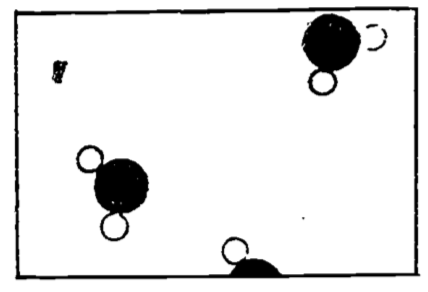
\includegraphics[width=0.5\linewidth]{figures/fig-physics-1} \caption{Water vapor (steam) (from Feynman 1963).}\label{fig:fig-physics-1}
\end{figure}

If we imagine that Fig. \ref{fig:fig-physics-1} is an enlarged photograph of a portion of a vessel containing water molecules only, we would infer that the water was in the vapor state, or steam, since we see so few water molecules.

\begin{figure}
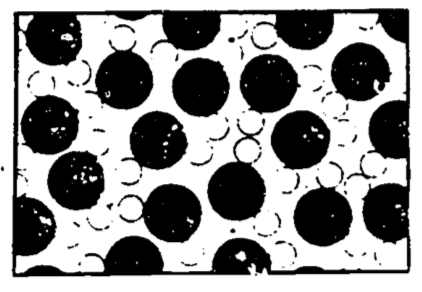
\includegraphics[width=0.5\linewidth]{figures/fig-physics-2} \caption{Water (liquid) (from Feynman 1963).}\label{fig:fig-physics-2}
\end{figure}

Figure \ref{fig:fig-physics-2} shows the molecules as they might appear when in the liquid state. Here the molecules are relatively closely packed, but still in a jumble. This state might have been arrived at from the previously illustrated vapor state by several means. We might have just added more steam molecules to force the molecules to be closer to each other (by increasing the density). (We would be required to do this at a higher pressure than existed already in the vessel, else more molecules would leave the vessel than enter it when we were trying to add some molecules.) We might only have decreased the volume of the vessel by forcing a piston into it---this gets the molecules closer together by increasing the density and hence the pressure without adding more molecules. Or we might simply have lowered the temperature of the vessel; this slows down the molecules sufficiently that the attractive forces between them are not overwhelmed by the energy of their motion, and permits groups of molecules to affiliate (or condense out of the vapor) whereupon these groups will respond to the earth's gravity and join other such groups at the bottom of the vessel in a puddle of water.

If we wait long enough at some appropriate conditions of pressure, temperature, and volume, a so-called equilibrium of the liquid and its vapor will come to pass (if the vessel is isolated). This doesn't mean everything has stopped. On the contrary, the molecules in both the liquid and vapor states are moving and jiggling violently about. Those molecules in the vapor state experience little force from other molecules, though occasionally they bang into each other or return to the surface of the liquid. Those molecules in the liquid state are held in the liquid by fairly strong attractive forces from their neighbors, but occasionally they gather enough velocity to escape the liquid into the vapor. Equilibrium is said to occur when the average number escaping the liquid per unit time equals the average number returning to the liquid per unit time. If the vessel is open to the atmosphere, those water molecules which have escaped from the liquid will not be likely to return, and eventually all the liquid will evaporate.

The average velocity of the molecules determines the \emph{temperature} of the substance, the higher the velocity the higher the temperature. When a ``hot'' object is placed against a ``cold'' object, some of the faster (or more highly energetic) molecules of the hot object will collide with the less energetic molecules of the cold object, the net effect being that the ``hot'' molecules slow down and the ``cold'' molecules speed up. In this event we will say that \emph{heat} energy has been transferred from the hot to the cold object. Notice from the preceding paragraph, that when the liquid is evaporating, it is the molecules with the higher energies that escape the liquid, leaving relatively lower energy molecules behind. Thus if the vessel is open, so that these high energy molecules are unlikely to return, the liquid will cool. This cooling of the liquid can be sped up by immediately removing newly escaped ``hot'' molecules in order to prevent their return, such as by blowing them away. ``Hence, blow on soup to cool it!'' (Feynman 1963).

Figure \ref{fig:fig-physics-3} shows a two-dimensional (and hence wrong, except qualitatively) representation of a three-dimensional crystal of ice. An important feature of this diagram is that each molecule has its ordered position in a periodically repeating array. Do not be led by this to believe that the molecules are held so tightly in place as not to be moving.

\begin{figure}
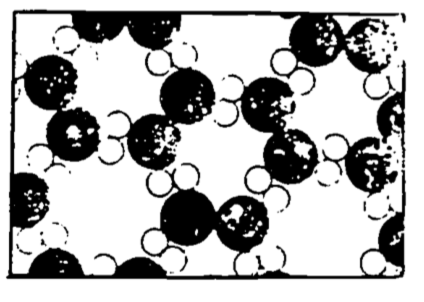
\includegraphics[width=0.5\linewidth]{figures/fig-physics-3} \caption{Ice (from Feynman 1963).}\label{fig:fig-physics-3}
\end{figure}

They surely are not free to slide and move among each other, but they are vibrating in place, so that an occasional molecule can by chance receive sufficient energy from its neighbors to escape the surface of the ice. Notice also the ``openness'' of this crystal structure, which is partly a consequence of the 105° angles between the hydrogen atoms of the water molecule. When the temperature of the ice is raised to the point where the vibrational energy of the individual molecules breaks the hydrogen bonds (i.e., when the ice melts), the molecules are free to slip into the more closely packed (albeit less structured) liquid arrangement. Water is more dense than ice---hence, ice floats! This is a peculiar property of water (since the solid for most substances is denser than the liquid state) and is of great biological significance.

As the surface water of a lake cools ice forms and floats to the surface. The ice thus formed serves as an insulator against continued, otherwise rapid, freezing of the water below it. In other words, heat transfer from the water to the cold winter environment must take place through an increasingly thicker layer of ice, which greatly slows the freezing of the lake, contrary to what would happen if the ice sank, leaving the surface of the lake constantly exposed to the cold. Thus life in the lake is preserved under the ice layer. Additionally, if ice sank to the bottom, then in spring and summer thawing the heat transfer would have to take place through an increasingly larger insulating layer of water. In fact, many lakes in north temperate climes would likely never thaw, especially after several years of this process permitted the bottom ice layers to build up.

We now have an inkling of the power of the atomic hypothesis. We begin next a discussion of the basic force laws of physics, and will continue to invoke the atomic hypothesis in the ensuing discussions.

\hypertarget{basic-force-laws}{%
\section{BASIC FORCE LAWS}\label{basic-force-laws}}

The ``stage'' on which inorganic or organic processes take place was thought before 1905 to be the ordinary three-dimensional space of Euclidean geometry, with change occurring in a medium called ``time.'' Einstein, in his theory of relativity, demonstrated the need for us to reshape our notions of space and time, since in different frames of reference (moving at different velocities with respect to each other), lengths and times will differ. Events which seem to occur simultaneously in one frame will not appear to be simultaneous to an observer in another frame. Relativity is of course a rather heady subject, and one which we won't discuss further, but it points up the difficulties which arise in defining precisely and appreciating the most basic quantities in physics.

A notion of what ``time'' is, for example, is so ingrained in our everyday experience, that we hardly think it necessary to define it. (PROBLEM: Try to define time!) The best the dictionary seems able to do is to define time as the ``\emph{period} during which an action, process, etc., continues; measured or measurable \emph{duration}.'' (Emphasis added.) Thus ``time'' is a ``period,'' or a ``duration.'' What, pray, is a ``period'' or a ``duration?'' We may invent some more synonyms, but eventually we find ourselves caught in a circular definition\ldots time is time (and then you wave your hand and say ``You know what I mean!''). We are just going to have to content ourselves with this, provided we can give a fairly precise means of measuring that which we call ``time.'' One way is to divide the period of rotation of the earth into 86,400 equal parts and call it the ``second.'' This has been found to be insufficiently accurate for many reasons (one is that the earth is \textbf{not} that constant a clock). In 1960, the ``second'' was defined in an international agreement to be a certain fraction of the particular year beginning on the vernal equinox of 1900, ending on the vernal equinox of 1901. This being a rather difficult standard to move about from laboratory to laboratory (you can't even go to Paris for it!), a recent definition has been provisionally accepted based on the number of oscillations of the cesium atom.

Without attempting to give a verbal definition of length (``You know what I mean!''), we give you the standard length of one meter, which was formerly defined to be the distance between two scratches on a platinum-iridium bar kept in Paris and measured under standard conditions of temperature and pressure. This standard was based on an old measure of the earth's circumference, thought to have been 40,000 kilometers on a great circle passing through Greenwich, but the standard is now based on the wavelength of a particular line in the emission spectrum of krypton 86. This new primary standard is a more reproducible standard than the Pt-Ir bar (How wide is the scratch on the Pt-Ir bar? How closely can standard temperature and pressure be held?), and a more convenient measure since it can be maintained in one's own laboratory for about the cost of three or four round trip fares to Paris.

The ``actors'' on our ``stage'' of three-dimensional space plus time are particles---atoms, molecules, protons, neutrons, electrons, etc. The particles are characterized by several fundamental properties, which when fully understood should, in theory at least, allow us to comprehend the most complicated of life processes. These properties (expressed as the \emph{forces} which particles exert on each other) are surprisingly few in number; there are four basic force laws, (1) gravitational, (2) electromagnetic, (3,4) weak and strong nuclear, which are used in conjunction with the law of ``inertial force'' and which embrace all of what the physicist understands of the universe today. (There may be more force laws forthcoming, e.g., a law describing the force holding the constituent parts of a proton together, but it's not likely that any newly discovered force laws will have a strong bearing on life processes.)

The atomic theory in conjunction with a knowledge of the force laws will allow us to view a gas as a collection of moving particles, whose pressure is the result of collisions of these particles with the walls of its containing vessel, or perhaps with your eardrums. We will be able to calculate pressure in terms of the ``inertial force'' (i.e., the change in momentum of the molecules as they bang into the wall and reverse their direction). The drift of the particles, if they're all moving in one direction, will be called \emph{wind}. If the motion of the particles is \emph{random}, we shall call it \emph{heat}. Ii the motion is in waves of excess density occurring at a regular frequency, we will know it as \emph{sound}, whose pitch we'll discover depends on the frequency.

The understanding of these things based on so few underlying principles, is a remarkable achievement. We shall proceed by discussing the notions of mass and force, and then by describing the force laws.

\hypertarget{inertia}{%
\subsection{Inertia}\label{inertia}}

In just the same way that ``time'' and ``length'' were so difficult, in fact impossible, to provide true definitions for (in the mathematical sense of definition), we shall find that ``mass'' and ``force'' must also be defined with some hand-waving. The student should not despair---this is not the fault of physics, nor of this presentation---it's just the way life is. Even the mathematician must face up to a fundamental imperfection in his otherwise perfect discipline. For mathematics must eventually trace all of its definitions back to some primitive concept, the universally accepted primitive concept being that of the ``set.'' What is a ``set'' of objects? Well, it's a ``collection'' of them. What's a collection? It's a ``group.'' Et cetera. Eventually we use up all our synonyms for ``set,'' and return to\ldots{}``set.'' The definition is circular. Thus mathematicians rely on grasping intuitively, without precise definition, the notion of set. Once that is accepted, of course, mathematics is on sound footing.

Thus we shall simultaneously introduce the ideas of force and mass (and hence, inertia) by presenting Newton's first and second laws:

Newton's first law (law of inertia): Every body will remain in a state of uniform motion unless acted on by external force.

Newton's second law: The acceleration of a particle is directly proportional to the resultant external force acting on the particle, is inversely proportional to the mass of the particle, and has the same direction as the resultant force.

The second law is usually written:
\begin{equation}
F=ma
\label{eq:physics-1}
\end{equation}
where\\
\hspace*{0.333em}\hspace*{0.333em}\hspace*{0.333em}\hspace*{0.333em}\hspace*{0.333em}\hspace*{0.333em}\(a\) = acceleration (change in velocity per unit time)\\
\hspace*{0.333em}\hspace*{0.333em}\hspace*{0.333em}\hspace*{0.333em}\hspace*{0.333em}\hspace*{0.333em}\(m\) = mass\\
\hspace*{0.333em}\hspace*{0.333em}\hspace*{0.333em}\hspace*{0.333em}\hspace*{0.333em}\hspace*{0.333em}\(F\) = force

If we know the meaning of position and time, then velocity (time rate of change of position, meters/sec) and hence acceleration (time rate of change of velocity, meters /sec\textsuperscript{2}) give us no problem. Let us say for the moment that we have some intuitive sense of what ``mass'' is. In fact, let us ``define'' one kilogram of mass to be the ``quantity of matter'' in a certain cylinder of platinum-iridium alloy preserved at the International Bureau of Weights and Measures in Paris, and let us measure unknown masses by balancing them opposite this standard (both masses presumably being acted on by the same ``force'' due to gravity).

We then might be inclined to ``define'' force in such a way that Newton's second law holds. That is, if we observe that a body is either at rest or moving in a straight line at constant velocity (what's a straight line?), we will say that no net force is acting on the body. Or contrariwise, that if the body is accelerating, then a net force must be acting on the body. This has the effect of rendering Newton's second law as a mere definition with no physical content, and hence not an experimentally verifiable law of physics. However, the real content of Newton's laws is supposed to be this: ``that the force is supposed to have some \emph{independent properties}, in addition to the law \(F = ma\); but the specific independent properties that the force has were not completely described by Newton or by anybody else, and therefore the physical law \(F = ma\) is an incomplete law. It implies that if we study the mass times the acceleration and call the product the force, i.e., if we study the characteristics of force as a program of interest, then we shall find that forces have some simplicity; the law is a good program for analyzing nature, it is a suggestion that the forces will be simple'' (Feynman 1963, Ch. 12). Furthermore, there is the implication that forces are of material origin, that if a body is observed to accelerate, we will find some physical body nearby which is the source of that force. Thus we must consider simultaneously with Newton's second law, the force laws associated with the nearby presence of matter.

This we'll do, upon noting that if Newton's second law holds, we may assign the units to force of the right-hand side of the expression, kg m/s\textsuperscript{2}, and since this is a clumsy unit, we shall call it the ``newton'':

1 newton (nt) \(\equiv\) 1 k m/s\textsuperscript{2}

\hypertarget{gravitational-force}{%
\section{GRAVITATIONAL FORCE}\label{gravitational-force}}

The story of gravitation begins with the ancients observing the motions of the planets among the stars, and eventually concluding that they went around the sun, a fact much later picked up by Copernicus. Tycho Brahe had the revolutionary idea (at least by comparison to the ancients) that one could measure the movements of the planets and establish their paths in space, which then might resolve the arguments as to whether they indeed moved around the sun. Tycho made extensive measurements, which Kepler then used to establish his three famous laws: (1) planets move in ellipses, with the sun at one focus, (2) the radius vector from sun to planet sweeps out equal areas in equal times, and (3) the period of revolution about the sun is proportional to the 3/2 power of the semimajor axis of its orbit.

Galileo also studied the laws of motion, coming up with the principle of inertia (that undisturbed bodies coast forever in a straight line), which Newton extended by introducing the notion of force, which it was necessary to apply in order to either speed up or slow down the body, or perhaps to cause it to deviate from a straight line path.

In the process of his theoretical studies on the motion of planets, Newton invented the calculus, from which he was able to show that Kepler's second law on equal areas being swept out in equal times followed from the assumption that the forces on the planets were directed exactly toward the sun. Furthermore, Kepler's third law was found to require that the force diminish with distance from the sun, in fact that the force had to be inversely proportional to the square of the distance from the sun. Finally, Newton proposed that the phenomenon of gravitation was universal, that everything attracts everything else, and used this with his inverse square law to demonstrate that the planets must move in accordance with Kepler's first law, in ellipses about the sun, as must any smaller body (such as a moon) about its parent body (say a planet).

Newton's law of universal gravitation is:
\begin{equation}
F=G\frac{m_1m_2}{r^2}
\label{eq:physics-2}
\end{equation}

where\\
\hspace*{0.333em}\hspace*{0.333em}\hspace*{0.333em}\hspace*{0.333em}\(F\) = force of one body on the other (newtons)\\
\hspace*{0.333em}\hspace*{0.333em}\hspace*{0.333em}\hspace*{0.333em}\(m_1,m_2\) = masses of the two bodies (kilograms)\\
\hspace*{0.333em}\hspace*{0.333em}\hspace*{0.333em}\hspace*{0.333em}\(r\) = distance between the two bodies (meters)\\
\hspace*{0.333em}\hspace*{0.333em}\hspace*{0.333em}\hspace*{0.333em}\(G\) = gravitational constant = 6.670 \(\times\) 10\textsuperscript{-11} nt m\textsuperscript{2}/kg\textsuperscript{2}

This force is the weakest of the four known basic force laws. We tend only to notice its existence when at least one of the masses is very large, such as the earth is, and often don't realize that all masses attract each other gravitationally (which, of course, is why it's known as a ``universal'' law). At the molecular level, gravity plays an insignificant role in life processes (where electrical forces, which are about 10\textsuperscript{40} times as powerful as gravity, are the most important). However, on a macroscopic scale, gravity plays an important role in determining structure and function of organisms, and ultimately limits the size of large animals (with the result that the largest of earth's creatures are aquatic, where the buoyant force of water opposes the force of gravity; and which dictates, in general, that aquatic creatures have lower energy requirements than terrestrial forms).

The weakness of gravity makes the determination of \(G\) tricky. Cavendish was the first to successfully measure \(G\) in the laboratory, which he did with an apparatus called a torsion balance. It consists of a horizontal arm suspended by a thin torsion fiber. Lead balls on each end of the arm are gravitationally attracted to a pair of large stationary lead balls, which applies a twist to the fiber in proportion to the force.

PROBLEM 1:\\
Cavendish claimed to be ``weighing the earth'' by his experiment. Using Newton's second law in combination with his law of universal gravitation, and using the facts that the acceleration due to gravity at the surface of the earth is g = 9.81 m/s\textsuperscript{2}, and the radius of the earth is 6368 km, compute the mass of the earth. (In solving this problem, assume the mass is all at a point in the center of the body. It is a remarkable truth, as proved by Gauss, that as long as the bodies possess spherical symmetry, this gives the correct answer.)

\hypertarget{electromagnetic-force}{%
\subsection{Electromagnetic Force}\label{electromagnetic-force}}

The classical theory of electromagnetism as it was ultimately developed in the 19th century, and which culminated in Maxwell's synthesis of the laws of electricity and magnetism with those laws of the behavior of light, is one of great beauty and also of great complexity. It is too complicated to present here in entirely correct detail, but though the formulas we give are approximations, they will suffice for our purposes of understanding something of life systems.

As students of cellophane laundry bags have observed in dry weather, there seems to be an entirely different sort of force from gravity, one which is strongly attractive between the bag and the hairs of one's forearm. More diligent students have experimented with hard rubber rods and cat's fur, glass rods and silk, and have discovered that there must be two different kinds of matter, which we call ``positive'' and ``negative,'' such that two ``positives'' or two ``negatives'' repel each other, while ``positive'' and ``negative'' matter will attract one another. We say hard rubber becomes negatively \emph{charged} when rubbed with cat's fur, and glass becomes positively charged when rubbed with silk. We now know that \emph{electrical charge} is a property of the constituents of the atom, positive electricity defined to be associated with the nuclear proton, and negative electricity associated with the orbital electron. Furthermore, the charge on the rubber and glass rod gets there by transferring electrons from the cat's to the rubber, and from the glass rod to the silk.

In 1785, Coulomb discovered with the use of a torsion balance that, like gravity, the force between charged bodies varies inversely as the square of the distance between them. Nowadays, Coulomb's electrostatic force law is written:
\begin{equation}
F=\frac{1}{4\pi\varepsilon_o}\frac{q_1q_2}{r^2}
\label{eq:physics-3}
\end{equation}
where\\
\hspace*{0.333em}\hspace*{0.333em}\hspace*{0.333em}\hspace*{0.333em}\(F\) = force (newtons)\\
\hspace*{0.333em}\hspace*{0.333em}\hspace*{0.333em}\hspace*{0.333em}\(r\) = distance between charges (meters)\\
\hspace*{0.333em}\hspace*{0.333em}\hspace*{0.333em}\hspace*{0.333em}\(q_1,q_2\) = charge on bodies 1 and 2 (coulombs)\\
\hspace*{0.333em}\hspace*{0.333em}\hspace*{0.333em}\hspace*{0.333em}\(\frac{1}{4\pi \varepsilon_o}\) = 8.987 \(\times\) 10\textsuperscript{9} \(\frac{nt\cdot m^2}{coul^2}\)

The unit of charge, the coulomb, is formally defined today in terms of the amount of silver deposited on an electrical terminal under a certain electrical current, but for the purposes of this module it will be easier to define the coulomb in such a way that the magnitude of the charge \((e)\) on an electron (which is \emph{exactly} the same in magnitude as the charge on a proton) is given by:

\[e=1.6019\times10^{-19}coul\]
The coulomb is one of the five fundamental units (length, time, mass, electrical charge, and temperature) in terms of which \emph{all} physical units may be expressed. The constant of proportionality (\(\frac{1}{4\pi\varepsilon_o}\)) is arbitrarily assigned this strange form by physicists so that certain other of their expressions derived from Coulomb's law are more aesthetic in appearance than they otherwise would be.

PROBLEM 2:\\
Determine the repulsive force between two electrons placed at a distance of 1 mm from each other.

PROBLEM 3:\\
Determine the attractive force due to gravitation between the above two electrons (mass of electron \(- 9.107 \times 10^{-31}\)kg). Hence demonstrate that for electron the electrical force is about 10\textsuperscript{42} times as strong as the gravitational force.

As the above problems illustrate, the magnitude of the electrostatic force is enormous. Yet in our everyday experience the balance between negatively and positively charged matter (electrons and protons) is so nearly perfect in most objects that we fail to notice it. In fact, if you were standing at arm's length from someone, and each of you had one percent more electrons than protons, the repulsive force between you would be sufficient to lift a weight equal to that of the earth (Feynman 1963).

Despite the near-perfect macroscopic balance of electrons and protons, if a small volume of matter is viewed at the atomic scale, electrons and protons are not present in equal numbers and do not balance out over the volume. Thus there are strong residual electrical forces which give the neutral atom its integrity and which account for the rigidity and strength of most solid materials.

Under the strong attractive force between them, electrons and protons try to get as close to each other as they can, up to a certain limit. To understand why they don't get closer to each other than they do (\textasciitilde10\textsuperscript{-8} cm) requires a knowledge of quantum mechanics beyond the scope of this set of modules. Suffice it to say that if the electron were confined in a region too close to the nuclear protons, Heisenberg's uncertainty principle would require the electron to possess a large momentum which would effectively keep it out of the nucleus (most of the time!).

But what holds the protons together in such close proximity in the nucleus? The repulsive electrostatic force between two or more protons is just huge at sub-nuclear distances (\textasciitilde10\textsuperscript{-13}cm). The answer is that there is another basic force which keeps the nucleus together, and which must be attractive and more powerful than the electrostatic force. This is called the \emph{strong nuclear force}, which along with another weaker-than-electrostatic force called the \emph{weak nuclear force}, comprises the third and fourth basic force laws and completes the description of all the basic force laws known to physicists today. We shall not discuss these last two laws further, other than to say that they are not ``inverse square'' laws, but rather act only over very short distances. The strong nuclear force is not appreciable in magnitude beyond distances roughly equal to the diameter of a uranium nucleus. In fact, the uranium nucleus with its 92 protons and its approximately 145 neutrons, is on the verge of flying apart under electrostatic repulsion. A small nudge, as might be given it by smacking into a low energy neutron, will cause it to fly apart (fission) and release the electrical energy (commonly, but erroneously, called ``nuclear energy'') stored in the close proton-to-proton affiliation.

We have described the law of interaction between charges at rest. To complete our description of electrical forces in this module, we must set down the law by which forces act between charges in motion. This is the phenomenon of magnetism, which when coupled with the law for electrostatics (and in fact we know now from the special theory of relativity that they are inseparable) forms the basis for what we term electromagnetic phenomena. The description of the magnetic force is difficult without introducing the intermediary concept of a magnetic field (it's difficult enough even this way!). It goes like this: (1) a moving charge sets up what we call a \emph{magnetic field}; (2) another charge in motion experiences a force as it moves through this magnetic field.

The Biot-Savart law (sometimes called Ampere's law) describes the magnetic field set up at a distance \(r\) from moving charges (current) in a wire (see Fig. \ref{fig:fig-physics-4}):
\begin{equation}
dB=\frac{\mu_o\;i\;dl\;sin\theta}{4\pi r^4}
\label{eq:physics-4}
\end{equation}
where\\
\hspace*{0.333em}\hspace*{0.333em}\hspace*{0.333em}\hspace*{0.333em}\(dB\) = incremental magnetic field (weber/m\textsuperscript{2})\\
\hspace*{0.333em}\hspace*{0.333em}\hspace*{0.333em}\hspace*{0.333em}\(i\) = electric current (coul/s \(\equiv\) ampere)\\
\hspace*{0.333em}\hspace*{0.333em}\hspace*{0.333em}\hspace*{0.333em}\(dl\) = incremental length of current carrying wire (m)\\
\hspace*{0.333em}\hspace*{0.333em}\hspace*{0.333em}\hspace*{0.333em}\(r\) = distance from \(dl\) to point where \(dB\) is measured (m)\\
\hspace*{0.333em}\hspace*{0.333em}\hspace*{0.333em}\hspace*{0.333em}\(\theta\) = angle between \(dl\) and \(r\)\\
\hspace*{0.333em}\hspace*{0.333em}\hspace*{0.333em}\hspace*{0.333em}\(\frac{\mu_o}{4\pi}\) = 10\textsuperscript{-7} weber/amp-m

The units for magnetic field \((B)\) will be seen from Equation \eqref{eq:physics-5} (next page) to be nt-sec per coul-m, which is conventionally called weber/m\textsuperscript{2} instead.

\begin{figure}
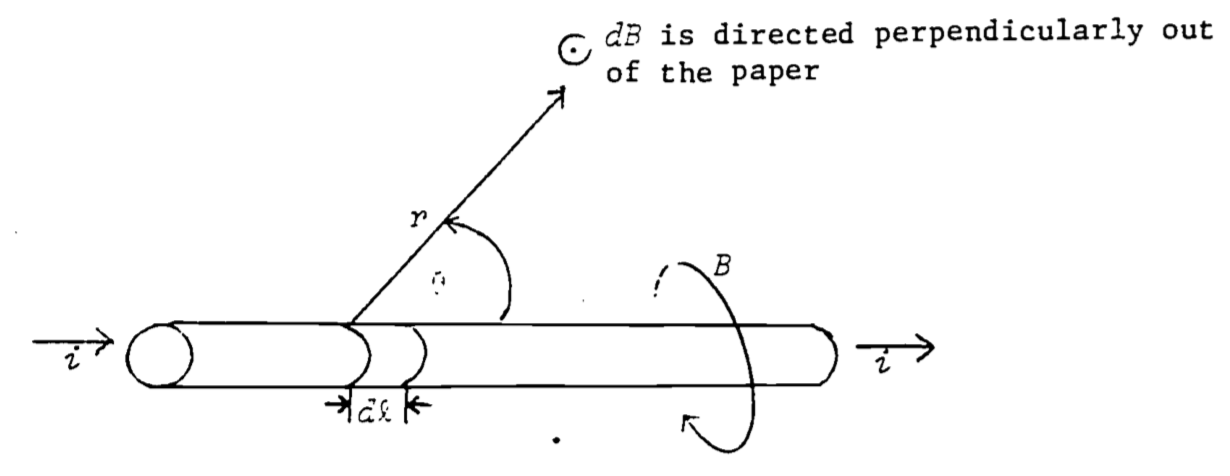
\includegraphics[width=0.75\linewidth]{figures/fig-physics-4} \caption{Magnetic field produced by current-carrying wire (Biot-Savart)}\label{fig:fig-physics-4}
\end{figure}

If the thumb of your right hand is pointed in the direction of the current, the magnetic field circles about the wire in the direction of the fingers of your right hand.

PROBLEM 4:\\
Compute the total magnetic field at the point in Fig.\ref{fig:fig-physics-4} by summing (integrating) the contribution from all elements \(dl\), in a very long wire carrying current \(i\). (Assume the point is a perpendicular distance \(R\) from the wire.)\\
The force on a charge \((q)\) moving through a magnetic field \((B)\) is given by:

\begin{equation}
F=qvBsin\Psi
\label{eq:physics-5}
\end{equation}

where\\
\hspace*{0.333em}\hspace*{0.333em}\hspace*{0.333em}\hspace*{0.333em}\(F\) = force (nt)\\
\hspace*{0.333em}\hspace*{0.333em}\hspace*{0.333em}\hspace*{0.333em}\(q\) = charge (coul)\\
\hspace*{0.333em}\hspace*{0.333em}\hspace*{0.333em}\hspace*{0.333em}\(v\) = velocity of charge (m/s)\\
\hspace*{0.333em}\hspace*{0.333em}\hspace*{0.333em}\hspace*{0.333em}\(B\) = magnetic field (weber/m\textsuperscript{2})\\
\hspace*{0.333em}\hspace*{0.333em}\hspace*{0.333em}\hspace*{0.333em}\(\Psi\) = angle between velocity vector and \(B\) (as \(v\) rotates into \(B\)).\\
The direction of the force is as shown in Fig. \ref{fig:fig-physics-5}.

\begin{figure}
\includegraphics[width=0.75\linewidth]{figures/fig-physics-5} \caption{Force on charge moving through constant magnetic field.}\label{fig:fig-physics-5}
\end{figure}

In other words, if the fingers of the right hand follow \(v\) as it rotates into \(B\), the thumb points in the direction of the force (true for positive charge--negative charge changes the sign of the force vector).

It is worth noting that all of what is now known as classical electromagnetic theory was summarized by Maxwell into four compactly written vector differential equations (beyond the scope of these modules!), cleverly called Maxwell's equations, which when solved by Maxwell led him to the following conclusion:

If two charges are initially held a distance \(r\) from each other, and at time 0 one of the charges is made to jiggle up and down with a frequency \(f\), the second charge will eventually experience a force on it which changes at the same frequency \(f\) with which the distance between the two charges is varying. But it will \emph{not} experience this changing force immediately at time 0! The news that the first charge has started to jiggle does not arrive until \(\frac{r}{v}\) seconds after the jiggling has begun, where \(v\) is the velocity at which the news travels, and which was predicted by Maxwell's equations to be:

\[v=\frac{1}{\sqrt{\mu_o\varepsilon_o}}=\sqrt{8.987\times10^9\times10^7}=2.998\times10^8m/s\]
\[=c=\;\mbox{velocity of light}\]
Note that \(\varepsilon_0\) and \(\mu_0\) were measured in the laboratory under static conditions as the proportionality constants in Coulomb's and Biot-Savart's laws, respectively. This seemingly remarkable coincidence, that electromagnetic radiation travels at the same speed at which light had been previously found to travel, led Maxwell to the inevitable conclusion that light was an electromagnetic phenomenon, which of course has been borne out. We now know that the light which we see is caused by the frantic jiggling of electrons, the color we see depending on the frequency of the jiggling. The electromagnetic spectrum extends far beyond the ability of our eyes to see however, ranging (in practical terms) from the very low frequency waves used in long-distance radio communication, through the higher frequency television and radar waves, through the infra-red (heat), visible, and ultraviolet, to X-ray and \(\gamma\)-ray frequencies. The study of the interaction of electromagnetic radiation of different frequencies with matter, its absorption, transmission, and reflection as dependent on the chemical make-up of the matter and the frequency of the radiation, has long occupied the physicist and is of central importance to the proper design of a living organism, plant or animal, enabling it not only to cope with its thermal environment but to sense the presence of its food or its enemies. Other modules also discuss this interaction and its importance in greater detail.

In conclusion, the electromagnetic forces are by far the most important of any of the basic force laws in understanding the living organism. Atomic processes, whether they be the ``physical'' processes involved in changes of state\ldots solid, gas, or liquid\ldots or the ``chemical'' processes involved in exchanges of partners between atoms, are basically manifestations of the electromagnetic force laws (sometimes necessarily being modified by the rules of quantum physics). Certain other processes, such as elastic collisions between molecules or between large objects, hence friction, are really the result of an electrostatic repulsion between molecules at close range. In short, most of biophysics and biochemistry could ultimately be explainable (in theory, at least!) by an elaborate application of Maxwell's classical laws and those of modern quantum electrodynamics.

\hypertarget{other-force-lawsfriction-intermolecular-forces-hookes-law}{%
\subsection{Other Force ``Laws''--Friction, Intermolecular Forces, Hooke's Law}\label{other-force-lawsfriction-intermolecular-forces-hookes-law}}

There are other so-called force laws which are usually treated in elementary presentations, which, though apparently having a reality of their own, are seen on closer inspection to be consequences of the basic laws of electromagnetism. For example, the frictional ``drag'' force on a body moving through a fluid (liquid or gaseous) is observed to be proportional to the velocity of the body relative to the fluid if the velocity is slow enough that no turbulence is present. At higher velocities, the force opposing the motion may be more nearly proportional to the square of the velocity. This is the case when an airplane flies through the atmosphere at subsonic speed. The frictional force ``law'' is actually a consequence of the molecules of the fluid bombarding the object, changing their momentum during the act of collision, which is in turn a consequence of the strong repulsive electrostatic force between two molecules as they approach too closely. The sum of the basic electromagnetic interactions between a myriad of molecules results in the measured drag forces in a manner so complicated that the frictional effects have never been calculated from first principles.

The force between two molecules requires a knowledge of quantum mechanics for a full understanding; nonetheless a good qualitative understanding of such forces can be couched in classical terms. It is necessary to consider cases, since many molecules have fundamental asymmetries, such that the mean positions of their negative and positive charges do not coincide. The water molecule serves as an example, where the negative charge tends to reside more on the oxygen, creating what we call a \emph{dipole}. Thus there are strong attractive forces between water molecules in a \emph{dipole-dipole interaction}.

Even in molecules where the mean positive and negative charges coincide (\emph{non-polar} molecules), such as is true in oxygen gas, the positive and negative charges do have some limited freedom to rearrange themselves, and this will happen in the presence of a nearby molecule. Since like charges repel and unlike charges attract, the charges rearrange themselves in such a way that the respective distances between like charges are slightly greater than the distances between unlike charges. The net repulsive force is therefore less (the like charges are farther apart) than the net attractive force (unlikes are closer together) and the molecules attract one another. Such a rearrangement is illustrated in Fig. \ref{fig:fig-physics-6}. It is known from the principles of quantum mechanics that non-polar molecules are attracted at long distances by a force which is inversely proportional to the seventh power of the distance, that is, \(F = \frac{k}{r^7}\). However, when the molecules get too close they repel one another with great force. These results are summarized in Fig. \ref{fig:fig-physics-7}.

\begin{figure}
\includegraphics[width=0.75\linewidth]{figures/fig-physics-6} \caption{Induced dipole-dipole interaction in otherwise non-polar molecules.}\label{fig:fig-physics-6}
\end{figure}

\begin{figure}
\includegraphics[width=0.75\linewidth]{figures/fig-physics-7} \caption{Force between two non-polar molecules as a function of the distance between then. A negative force implies attraction (redrawn from Feynman 1963)}\label{fig:fig-physics-7}
\end{figure}

As seen in Fig. \ref{fig:fig-physics-7}, there is a distance \(d\) at which there is neither attraction nor repulsion. This is where the molecules would remain in the absence of external forces. An attempt to push them closer together (to compress the substance) meets strong resistance. An attempt to separate them (to place the substance in tension) also meets resistance for a while, unless enough force is applied to break the bond (which fractures the substance). In a region around \(d\), the force of attraction or repulsion (due respectively to tension or compression) is very nearly linear, a law which holds true for many materials, and which is known as \emph{Hooke's Zara}:

\begin{equation}
F=kx
\label{eq:physics-6}
\end{equation}

where
~~~~\(F\) = force (nt)\\
\hspace*{0.333em}\hspace*{0.333em}\hspace*{0.333em}\hspace*{0.333em}\(x\) = distance from equilibrium (m)\\
\hspace*{0.333em}\hspace*{0.333em}\hspace*{0.333em}\hspace*{0.333em}\(k\) = proportionality constant (nt/m)

The various chemical interactions or exchanges of atoms between molecules are largely consequences of these and more complicated force laws (for more complex molecules) derivable from the basic laws of electromagnetism. The force laws by themselves however are not always so easy to work with. A much more elegant and deeper understanding of the interactions between molecules, and hence the life process, requires an understanding of the concept of energy, which we deal with next.

\hypertarget{energy}{%
\section{ENERGY}\label{energy}}

\hypertarget{work-and-potential-energy}{%
\subsection{Work and Potential Energy}\label{work-and-potential-energy}}

Suppose we carry a bucket of water up ten flights of stairs. We would probably all agree that some work had been done. If we had had a course in physics, we would be inclined to say that we had done some work on the bucket of water (as well as on our own selves) in carrying it up ten stories. From our everyday use of the word ``energy'' we might also note that we expended considerable energy in getting the bucket of water to that great height, and we might intuitively believe that in some way we have imparted some of that energy to the bucket of water, though of course it doesn't look any different to us from ten stories up as it did at ground level. We will be calling this energy which we endowed to the bucket of water, the ``potential energy,'' and justify this terminology by noting that if we were to open the window and pour out the water with careful aim onto the blades of a turbine at ground level, the energy of motion (i.e., the ``kinetic energy'') which the water builds up as it hurtles turbineward at an acceleration of 9.81 m/sec\textsuperscript{2}, will set the blades of the turbine in motion, which in turn will generate several milliwatt-hours of electrical energy. On our return to the ground floor we will no doubt be confronted by the chief physicist of the project who will deprecatingly inform us that though, while we were ten stories up we had a good deal of potential energy ourselves, in walking back down we had lost it all and had effectively performed no net work beyond that which we performed on the bucket of water (or on just the water if we brought the bucket back with us). The water itself, while no longer possessing potential energy, \emph{did} indeed convert that energy into some useful work in turning the blades of the turbine to produce electricity, but we did no useful work ourselves in descending the ten stories with the empty bucket.

Do physicists and physiologists have different ideas as to what work and energy are? Though it was a lot easier coming back downstairs with the empty bucket than it was going up with the full one, we know that it took some energy expenditure in getting back down the ten flights. And besides, if we had done no net work on ourselves, why do we need the food energy from a bologna sandwich before we can repeat the trip? To understand, we must become precise in our definitions, which we will do on the physicist's own terms (and which the physiologist will eventually find perfectly acceptable), and then we must bring these into accord with what we know must be true about our own bodily energy expenditure during the round trip.

If we slowly move an object a certain distance in a straight line, and if we must apply a force in the direction we move it (not counting the force necessary to overcome inertia---that's why we're moving slowly, so inertial ``force'' is negligible), the work done on the object by us is defined to be the force we applied, times the distance we moved, thus:
\begin{equation}
W=F_xx
\label{eq:physics-7}
\end{equation}
where\\
\hspace*{0.333em}\hspace*{0.333em}\hspace*{0.333em}\hspace*{0.333em}\(W\) = work (joules \(\equiv\) nt-m)\\
\hspace*{0.333em}\hspace*{0.333em}\hspace*{0.333em}\hspace*{0.333em}\(F_x\) = force in x-direction (nt)\\
\hspace*{0.333em}\hspace*{0.333em}\hspace*{0.333em}\hspace*{0.333em}\(x\) = distance (m)

When the distance traveled is great enough that the force is changing as we move the object (such as might be true if we took an object several thousand miles up, so that the force of gravity is diminishing appreciably as we move, or if the object were attached to a spring, where the force is proportional to the distance from equilibrium) we must modify the above definition by summing the infinitesimal amounts of work done in moving the object a series of infinitesimal distances (over each of which the force is essentially constant), which of course is equivalent to finding the integral:

\begin{equation}
W_{12}=\int_{x_1}^{x_2}F_xdx
\label{eq:physics-8}
\end{equation}

where \(x = x_1\) at the start of our travail, and \(x = x_2\) at the finish. Note that work is done only by that component of the force acting in the direction of motion. Any component for force perpendicular to the motion does no work under this definition.

If the path of motion is not straight, we must give the most general definition of work, which takes the form of a line integral (see Fig. \ref{fig:fig-physics-8}):
\begin{equation}
W_{AB}=\int_A^BFcos\theta ds
\label{eq:physics-9}
\end{equation}

where \(ds\) = incremental distance in direction of the path of travel\\
\hspace*{0.333em}\hspace*{0.333em}\hspace*{0.333em}\hspace*{0.333em}\(\theta\) = angle between F and direction of path.

Note that \(F cos \theta\) is the component of force in the actual direction of motion. Also note that the work done is computed from the force we must apply to the object, not from the force that is opposing our motion. (Otherwise it would have the opposite sign.)

\begin{figure}
\includegraphics[width=0.75\linewidth]{figures/fig-physics-8} \caption{Relations between F, $\theta$, and $d_s$ used in computing work in moving an object from A to B.}\label{fig:fig-physics-8}
\end{figure}

The actual calculation of a line integral is beyond the scope of this module, but this general definition of work is included for completeness.

Let's use the definition in order to compute the work done on the water in the bucket as we carry it up ten stories to a height \(h\) above the ground. The force due to gravity, which is acting downward on the water (of mass \(m\)), is equal to \(mg\). If we were to carry the water straight up (such as by climbing a vertical ladder) we would be applying an upward force mg, in the direction of motion. Thus the work we do on the water is force times distance, or:
\begin{equation}
W=mgh
\label{eq:physics-10}
\end{equation}

What if, instead of climbing a vertical ladder, we had carried the water up a plane inclined at the angle \((\phi)\) (Fig. \ref{fig:fig-physics-9})?

\begin{figure}
\includegraphics[width=0.75\linewidth]{figures/fig-physics-9} \caption{Relations between quantiles needed to calculate work against gravity on an object being taken up an inclined plane.}\label{fig:fig-physics-9}
\end{figure}

The vertical force we apply to the water is \(mg\), while the component of force acting in the direction of motion is \(mg sin\phi\). The distance the water moves under this constant force is \(\frac{h}{sin\phi}\). Consequently the work is:
\[W=mg\sin\phi\frac{h}{\sin\phi}=mgh\]
The same as before! This is no accident. In fact, it is not difficult to see that the amount of work done on an object in raising it a height \(h\), \emph{by any path}, will always be \(mgh\). (Imagine an arbitrary path from the ground to height \(h\) to be approximated by an interconnected collection of infinitesimally short straight line segments, the \(i^{th}\) one of which is tilted at an angle (\(\phi_i\) and rising an amount \(\Delta h_i\) over its length. The total work is thus \(\sum mg\Delta h_i = mgh\).) When a force law has the property that the work done on an object in moving it from position A to position B is the same no matter which path we take in getting from A to B, we call, the force \emph{conservative}. A corollary of this is that under a conservative force, a round trip from A to B and back to A again results in no net work being done. For if there were net work done in the round trip ABA, then all paths from A to B would not result in the same amount of work (since ABAB and AB are both legitimate paths from A to B, with the former clearly requiring more or less work when the round trip is thrown in).

When the force is conservative (as we have just shown to be true for a force which is constant in both magnitude and direction), then for an object of mass \(m\) each point in space will possess a unique value for the work required to move the object to that point from some constant reference point. This value of work is unique in the sense that no matter which path were chosen to get from the reference point to the position in question, we would do the same amount of work on the object. Of course if we shift the reference point, we may change the value of work in getting to the position in question. So when we pick a reference point, let's not change it. We may now regard an object of mass m at some position in space as possessing the property that a certain amount of work has been (or could have been) done on it in getting it from the reference point to where it is now. However, we don't usually call this property ``work'' (since ``work'' is an action). Instead, we refer to this property as the \emph{potential energy} of the object with respect to the reference point. Thus the potential energy of an object is the amount of work that would have to be done in taking the object from the reference point to its present location. To put it another way, the potential energy is the amount of work that the object could perform on something else in making its own way back to the reference point. Energy obviously has the same units as work (joules)---the two words are distinguished by our perception that ``potential energy'' is a \emph{property} possessed by a body (as a consequence of its position in space) which would enable it to perform \emph{an act} called ``work.''

The importance of our peculiar definitions of work and energy lies in the profound fact, which we will demonstrate subsequently, that under conservative force laws, the total energy of an isolated system remains constant. There may be exchanges of energy between certain parts of the system or there may be changes in form of the different energies (e.g., potential energy may be changed into the energy of motion), but the sum of all the component energies of the isolated system must remain forever constant.

Energy is recognized in several different forms, each associated with a different force law, and each expressed by a different formula. The different forms of energy we recognize are gravitational, kinetic, heat, elastic, electrical, chemical, radiant, nuclear, and mass-energy. Since there are only four basic force laws (taken in conjunction with Newton's second law), there is obviously some redundancy in this list. For example, what we call ``heat energy'' is in fact a manifestation of the ``kinetic energy'' (energy of motion) of the molecules of a substance.

Since the law of conservation of energy depends on the forces being conservative, it is well to ask whether the four basic force laws are conservative. They are indeed. There are no non-conservative forces! There are, however, some apparent non-conservative forces, such as friction. For example, if we slide an anvil from Dubuque to Peoria, the amount of work we do depends on which highways we slide it on. And surely if we make a round trip, we will do significantly more than zero work in getting back to Dubuque. Thus certainly our energy is not conserved. However, if we look at things more closely, we will discover that that work we did on the anvil, though not resulting in any potential energy gain by it, \emph{did} result in setting a number of molecules in both anvil and highway in much more rapid motion. Our work went into heating the highway and the anvil, that is, increasing the kinetic energy of their respective molecules and hence, increasing the temperature of both road and anvil-- it didn't result in what we think of as useful work, but neither did it result in a loss of energy to the universe.

If you are wondering whether this work against friction can be recovered to perform work on something else, that is, if we could use the enhanced kinetic energy of the Molecules of the anvil and the highway to do work, the answer is we could use some of it, but not all. A good deal of this energy will be forever unavailable to do work, which we will see later is a consequence of the second law of thermodynamics and which we shall have to elaborate upon in terms of what we call the ``entropy'' and ``free energy.''

We can now begin to understand some of the differences between ``physical work'' (as defined by Equation \eqref{eq:physics-9} and ``physiological work,'' such as we do when we run downstairs, or hold a heavy weight in a stationary position. In running downstairs, or at a constant level, though we're doing negative, or at best zero work against gravity, it seems apparent that we're doing considerable work against friction. Some of this results in a direct heating up of the environment---the air molecules we bump into are sped up, the molecules of the earth under our feet are given a jolt with each stride---but more significantly, there is a good deal of friction within our bodies as we run, many parts sliding and rubbing each other as our muscles contract and extend. We might think that since this energy remains within the body, in the form of kinetic energy, that it's not lost to us---we should still be able to get some useful work out of it. Again, the second law of thermodynamics denies this possibility for the most part, saying that we cannot get useful work solely by extracting energy from the kinetic energy of a randomly moving, i.e.~disordered, array of molecules. Thus, since the body cannot make good use of this energy, it must release most of it, or else this kinetic energy will result in a disastrous rise in body temperature. Consequently, water is made to appear on the surface of our skin through the pores (i.e., we sweat) and as we learned previously, the more highly energetic of these water molecules will depart, leaving behind the slower ones. And the body cools.

But there's more to the explanation of physiological work than just external and internal friction. For imagine that we're not running, but instead are standing as still as we can, while holding an anvil at chest height. There is no physical work being done, but there certainly is some physical exertion! If we were to set the anvil on a table, we know that neither physical work nor physical exertion would be required of the table. Why must we work so hard to do no physical work? The answer lies in the way our \emph{striated} or \emph{skeletal} muscles function.

Muscles consist of interdigitating protein filaments that slide past each other (Figs. \ref{fig:fig-physics-10} and \ref{fig:fig-physics-11}).

\begin{figure}
\includegraphics[width=0.75\linewidth]{figures/fig-physics-10} \caption{Muscle at rest.}\label{fig:fig-physics-10}
\end{figure}

\begin{figure}
\includegraphics[width=0.75\linewidth]{figures/fig-physics-11} \caption{Muscle contracted.}\label{fig:fig-physics-11}
\end{figure}

The energy which makes muscles contract comes mostly from the chemical energy stored in the molecular bond of a class of compounds called \emph{phosphagens}, the most noteworthy of which is adenosine triphosphate (ATP). The ATP will release its energy in the presence of calcium ions, which are stored away from the ATP in a system of tubules (the \emph{sarcoplasmic reticulum}) in the muscle cell. When an electrical signal from the nerve is delivered to a muscle fiber, the calcium ions in the sarcoplasmic reticulum are released into the fluid surrounding the muscle filaments. The ATP molecules present on these filaments release their chemical energy (by which we really mean electrical potential energy) and the muscle contracts, or at least attempts to. The calcium ions are immediately pumped back into the sarcoplasmic reticulum, and in fresh muscle, new ATP is created from another phosphagen present in muscle cells, which ultimately must get \emph{its} energy from the oxidation energy available from food combustion. These processes all happen in a matter of hundredths of a second, after which the muscle cell relaxes. So what we actually see upon the electrical signal from the nerve, is a twitch in the muscle fiber! For us to lift and hold a constant load, say the weight of an anvil, there must be many twitches per second---the nerves are constantly firing, and ATP is constantly discharging its energy and re-energizing. It can do so only as long as the blood can resupply the energy to the muscle from that energy available from food consumption. Under heavy exertion the energy from food consumption cannot be delivered fast enough to the muscle, and the load must be dropped or the running stopped for want of ATP. (As you might guess, there's more going on than just this, but these are the essential features.)

It seems strange that nature should have evolved such an inefficient scheme for muscle action, but apparently this is what we must give up in order to have ``fast'' muscle. Nature seems to have been unable to have evolved muscle which can act rapidly and also sustain large static loads. The smooth muscle (such as that surrounding the intestines) is built quite differently, and acts much more like the table in holding a constant load, where the molecules essentially lock into position to sustain that load. The abductor muscle of the clam represents a good example of smooth (hence ``slow'') muscle which can effortlessly sustain a load over long periods.

PROBLEM 5:\\
Determine the potential energy stored in a spring stretched from equilibrium a distance \(x\). (Recall, Hooke's Law is \(F = kx\).) Hooke's Law is, as you know, the same force law as that between two molecules at distances very near their equilibrium distance. This potential energy is a way of representing the vibrational energy of a diatomic molecule, which in the course of vibrating is rapidly exchanging potential energy (maximum at the maximum distance from equilibrium) for kinetic energy (maximum at the equilibrium distance).

\hypertarget{kinetic-energy}{%
\subsection{Kinetic Energy}\label{kinetic-energy}}

We must now formally obtain a formula for kinetic energy, which is defined to be the amount of work we do in overcoming the inertial force of a body of mass \(m\), in getting it from zero velocity to a velocity \(v\). The inertial force is given by Newton's second law, which we manipulate a bit using the chain rule for derivatives and recalling that the rate of change of velocity is acceleration:
\[F=ma=m\frac{dv}{dt}=m\frac{dv}{dx}\frac{dx}{dt}=mv\frac{dv}{dx}\]
We may insert this into the definition of work (Equation \eqref{eq:physics-8}) to get:
\begin{equation}
\mbox{Kinetic Energy}\equiv T=\int mv\frac{dv}{dx}dx=\int_0^vmvdv=\frac{1}{2}mv^2
\label{eq:physics-11}
\end{equation}
We are now ready to establish the law of conservation of energy, which we do forthwith.

\hypertarget{conservation-of-energy}{%
\subsection{Conservation of Energy}\label{conservation-of-energy}}

It's interesting to note that this cornerstone physics, the principle of conservation of energy, was first demonstrated by the German physician, Dr.~Julius Robert Mayer, based on his observation that the venous blood of a patient in the tropics is redder than the venous blood of a patient in the temperate zone. This difference, he concluded, resulted from the body's lower oxidation rate required to maintain body temperature in the tropics: Mayer viewed the organism not as an independent entity, but as a part of the environment and responsive to its external surroundings, which led him eventually to an understanding of the mechanical equivalent of heat, and ultimately to a statement of the law of conservation of energy, which he published in 1842 in Liebig's \emph{Annalen} on ``The Forces of Inorganic Nature.'' Thus did biology make a signal contribution to physical theory.

The principle of conservation of energy is simply stated:

\emph{In an isolated system, the total energy never changes.}

This is to say that if we are careful not to let anything bump into our system (such as air molecules), and if we keep it hidden from sources of radiant energy (such as the sun), then whenever we measure the kinetic and potential energies of the system's component parts, and add them up, we will always come up with the same answer.

For a single body acting under a conservative force, we may write one statement of the principle of energy conservation:
\[T + V = \mbox{constant}\]

where \(T\) and \(V\) are the respective kinetic and potential energies. A falling body, e.g., would every second be ``losing'' potential and ``gaining'' kinetic energies, but the total at any time is constant.

Let's see if this relationship holds in the case of a body of mass \(m\) falling freely in a gravitational field (neglecting frictional losses due to collision with air molecules). In such a case we would have:

\begin{equation}
\frac{1}{2}mv^2+mgh=\mbox{constant}
\label{eq:physics-13}
\end{equation}

If equation \eqref{eq:physics-13} is true then the time derivative of the left hand side must be zero. Taking this derivative:
\begin{align*}
\frac{d}{dt}(\frac{1}{2}mv^2+mgh)=\frac{1}{2}m\frac{d}{dt}(v^2)+mg\frac{dh}{dt}&=\frac{1}{\rlap{---}2}m\rlap{---}2v\frac{dv}{dt}+mg\frac{dh}{dt} \\
&=mv(-g)+mgv=0
\end{align*}

where we have chosen the positive direction for \(h\) to be upward, \(\frac{dh}{dt} = v\) (both \(\frac{dh}{dt}\) and \(v\) are negative), and the acceleration due to gravity \((\frac{dv}{dt} = -g)\) is a negative quantity since it is directed downward. Thus, the derivatives of both sides of \eqref{eq:physics-13} are zero and \eqref{eq:physics-13} is satisfied. We also interpret this to mean that the principle of conservation of energy is satisfied.

To show that conservation of energy holds in general is best done using the tools of vector analysis, which is beyond the scope of this module. It is easy to show without vector analysis that it must be true for an object moving in a straight line. Then if you're satisfied to think of an arbitrary curved path as being made up of infinitesimal straight line segments, you will be satisfied with the following:

All that need be done is to return to the development of the formula \eqref{eq:physics-11} for the kinetic energy, which was defined as the work necessary to get a body from zero velocity to a velocity \(v\). If we wish to find the work done \emph{on} the body in getting from a velocity \(v_1\) (at point 1 in space) to a velocity \(v_2\) (at point 2 in space), the steps are the same as in obtaining equation \eqref{eq:physics-11} except the final integral has limits \(v_1\) and \(v_2\):

\begin{align}
\mbox{Work in getting from 1 to 2} \equiv W_{12}&=\int_{v_1}^{v_2}mvdv \notag \\
&=\frac{1}{2}m(v_2^2-v_1^2) \notag \\
&=T_2-T_1
\label{eq:physics-14}
\end{align}

Equivalently, if the force acting on the body is conservative (work done is independent of path from 1 to 2), then we may figure out a potential energy (relative to an arbitrary point) of the body at each point, say and the work we must do \(V_1\) and \(V_2\), on the body in getting it from 1 to 2 is \(V_2 - V_1\). If we release the body at point 2, the force associated with the p(potential (let's say it's gravity) will do en amount of work \(W_{21} = V_2 - V_1\) on the body in getting it from point 2 to point 1. We may write:

\begin{equation}
W_{12}=-W_{21}=V_1-V_2
\label{eq:physics-15}
\end{equation}

Comparing this to equation \eqref{eq:physics-14} gives us the statement of conservation of energy:
\[V_1-V_2=T_2-T_1\]
or
\begin{equation}
T_1+V_1=T_2+V_2=\mbox{constant}
\label{eq:physics-16}
\end{equation}

since points 1 and 2 were arbitrary.

The principal assumption in this development is that the forces acting on the body are conservative, which we reiterate is true for all four known \emph{basic} force laws, but which is not necessarily true for other so called forces such as friction. Thus, when we employ the conservation principle, we must be sure that the system we have in mind is isolated, or else we must account for exchanges of energy between the system and its surroundings. Conservation of energy is a universal principle, but it works only if we have accounted for all possible exchanges of all possible forms of energy. We will discover that the laws of thermodynamics provide a most convenient tool for dealing with these exchanges.

In passing, we point out one more assumption made in the development of the law, which though not of professional interest to biologists, should be of some philosophical interest. In the development of the expression for the kinetic energy, the mass of the object was assumed constant. In everyday circumstances this is true, but as you're no doubt aware, at velocities near the speed of light it is not true. When Einstein used his formula for mass as a function of velocity in the development of an expression for kinetic energy, he discovered that in order for the formulation to be consistent with conservation of energy, a net change in mass in an isolated system would be associated with a net opposite change in energy of magnitude \(E = mc^2\), where \(m\) is the change in mass and \(c\) is the velocity of light. This is the form of energy previously referred to as mass-energy, and is of utmost importance to the under standing of nuclear reactions, though it won't concern us further here.

\hypertarget{gravitational-and-electrostatic-potential-energy}{%
\subsection{Gravitational and Electrostatic Potential Energy}\label{gravitational-and-electrostatic-potential-energy}}

We can now establish formulas for gravitational and electrostatic potential energy. For reasons that will become apparent in the development, we usually choose \(r = \infty\) to be the reference point for the potential energy; that is, we shall define \(V_{\infty} = 0\). Thus if we take equation \eqref{eq:physics-15} and \eqref{eq:physics-8} in combination to define potential energy, then substitution of equation \eqref{eq:physics-2}, Newton's law of universal gravitation, into the defining potential energy relations gives:
\begin{align*}
V_r-V_{\infty}&=-\int_r^{\infty}g\frac{Mm}{r^2}dr \\
V_r&=-G\frac{Mm}{r}
\label{eq:physics-17}
\end{align*}

where\\
\hspace*{0.333em}\hspace*{0.333em}\hspace*{0.333em}\hspace*{0.333em}\(M\) = mass of earth\\
\hspace*{0.333em}\hspace*{0.333em}\hspace*{0.333em}\hspace*{0.333em}\(m\) = mass of object whose energy we're computing\\
\hspace*{0.333em}\hspace*{0.333em}\hspace*{0.333em}\hspace*{0.333em}\(r\) = distance from center of earth

The negative sign is taken since the force is opposite to the positive \(r\) direction. Since we expect that an object loses gravitational potential energy as it falls closer to the center of the earth, and since we defined \(V_{\infty} = 0\), then we should expect \(V_r\) to be able to take on only negative values, and to be getting more negative as \(r\) becomes smaller. You may object that Newton's law of gravitation applies only to point masses (or infinitesimal masses) and that an accurate expression for the potential energy of an object at a distance \(r\) from the center of the earth could only be obtained from an integral over all the infinitesimal volume elements of the earth. Gauss, however, in a beautiful theorem, demonstrated that one could treat a spherical object as though all its mass were concentrated at the center, and get the exact answer that one would get by performing the complicated integration!

We have derived two different expressions for the potential energy in a gravitational field, which may have led to confusion. In the first case, we made the assumption that we were raising an object to relatively low heights (say no more than a few miles) over which distance the force of gravity could be considered constant. It was most convenient to consider the earth's surface as the zero reference point for computing the potential energy. In the second case we used the more accurate expression for the gravitational force, the form of which led to infinity as the most convenient reference point for computing potential energy. Since in any practical situation we will only be interested in change in potential energy, the choice of reference potential energy is immaterial, because no matter what reference point is chosen, the calculated \emph{change} in potential energy between two points will always be the same. We must not, however, change reference points in the middle of a calculation!

To demonstrate the power of the principle of conservation of energy, let's compute the ``escape velocity'' from the earth's gravitational field. Escape velocity will be defined as the velocity at which we must propel an object so that at a large distance the object is just barely moving. Thus at a great distance both the potential energy and kinetic energy will be zero. At the earth's surface, the total energy must therefore also be zero, allowing us to write:
\[\frac{1}{2}mv^2-G\frac{Mm}{R}=0\]
where \(R\) = radius of earth.

Thus the escape velocity is \(v = \sqrt{\frac{2GM}{R}}\).

PROBLEM 6:\\
Show that \(\frac{GM}{R^2}=g\), the acceleration due to gravity at the surface of the earth. Hence show that the escape velocity is approximately seven miles per second, knowing that \(g\) = 9.81 m/s\textsuperscript{2} and \(R\) = 6368 km.

Of greater biological importance is the potential energy associated with the electrostatic force. Since, like gravity, it is an inverse square law, there is no need to derive it again, but rather just write:

\begin{equation}
V=\frac{1}{4\pi \varepsilon_o}\frac{q_1q_2}{r}
\label{eq:physics-18}
\end{equation}

where once again infinity is chosen as the reference point. The sign is positive since, unlike gravity, the force between like charges is repulsive. (Of course, if the charges are unlike, we would come up with the negative energy associated with attractive forces.)

PROBLEM 7:\\
A glaucous-winged gull weighing 2 kg carries a cockle weighing 0.25 kg to a height of 10 m where at a horizontal flight speed of 3 m/sec it releases the cockle whose shell will shatter on the rocks below, as soon thereafter as possible to be devoured by the gull. What is the minimum energy that the gull could have expended in rising to 10 m and achieving its level flight?

PROBLEM 8:\\
At what speed will the cockle hit the ground?

PROBLEM 9:\\
The lowest energy state for the electron in the hydrogen atom has been measured to be -217.3 \(\times\) 10\textsuperscript{-20} joules. What is the radius of the hydrogen atom under this condition? (HINT: The centrifugal force" of a mass moving in a circular orbit is \(\frac{mv^2}{r}\). When this is equated to the electrostatic force holding the electron in orbit, a simple expression for the kinetic energy of the electron is obtained. Add this to the potential energy to get the total energy, which is -217.3 \(\times\) 10\textsuperscript{-20} joules. Solve for \(r\).)

With the background that we've now gathered, we are ready to begin a discussion of the application of the principles we've developed to the study of thermodynamics, which we will find to result in a most elegant set of tools for the handling of some otherwise vexing, but nonetheless important, biological problems.

\hypertarget{solutions-to-problems}{%
\section{SOLUTIONS TO PROBLEMS}\label{solutions-to-problems}}

\begin{enumerate}
\def\labelenumi{\arabic{enumi}.}
\tightlist
\item
  5.964 \(\times\) 10\textsuperscript{18} kg\\
\item
  2.306 \(\times\) 10\textsuperscript{-22} nt\\
\item
  5.532 \(\times\) 10\textsuperscript{-65} nt\\
\item
  \(\frac{\mu_0i}{2\pi R}\)\\
\item
  \(\frac{1}{2}kx^2\)\\
\item
  We substitute the relation \(\frac{GM}{R}=gR\) into \(v=\sqrt\frac{2GM}{R}\) to obtain \(v=\sqrt{2gR}\). Substituting, we obtain \(v=\sqrt{2*9.81*6368*10^3}\) m/s. We divide by 0.00062 to convert to miles/s. Obtaining v=6.93 miles/s.
\item
  205.2 J\\
\item
  39.73 m/s\\
\item
  0.530 \(\times\) 10\textsuperscript{-10} m. Hence the diameter of a hydrogen atom is 1.06 \(\times\) 10\textsuperscript{-10} m (or approximately 1 angstrom unit in an earlier terminology).
\end{enumerate}

\hypertarget{literature-cited}{%
\section{LITERATURE CITED}\label{literature-cited}}

Feynman, R.P., R. B. Leighton, and M. Sands. 1963. The Feynman Lectures on Physics. Addison-Wesley. Reading, Massachusetts.

\hypertarget{thermodynamicsintro}{%
\chapter{Thermodynamics Intro}\label{thermodynamicsintro}}

The First Law of Thermodynamics for Ecosystems

author: Stevenson, R. D.

\hypertarget{preface-4}{%
\section{PREFACE}\label{preface-4}}

This module and the subsequent companion module address how elementary concepts of thermodynamics can be applied to ecological processes. The First Law of Thermodynamics states that during any biological, physical, or chemical process, energy can neither be created nor destroyed. The relationship between an organism and its environment can be studied by examining the exchange of energy in the form of the flow of heat and the transfer of mass. The primary focus in the module is on the microclimate and the exchange of heat between organisms and their environment. The law is also used to study the energetic cost of locomotion, rate of food assimilation, and energy flow in ecosystems. A basic knowledge of algebra is required in order to understand the text and complete the problem set.

The First Law of Thermodynamics is discussed in this module both in its difference and differential forms. An undergraduate student in the life sciences with a background in algebra should be able to understand all of the material herein. The problem set should be worked as it extends as well as reviews concepts developed in the text.

\hypertarget{energy-exchange-of-organisms}{%
\section{ENERGY EXCHANGE OF ORGANISMS}\label{energy-exchange-of-organisms}}

This module develops elementary concepts of thermodynamics as they apply to ecological processes. The First Law of Thermodynamics deals with the conservation of energy and is of fundamental importance. It states that during any biological, physical, or chemical process energy can be neither created nor destroyed. This module and its companion ``Application of the First Law to Ecological Systems'' serve as a foundation for other modules in the thermodynamics series.

The relationship between an organism and its environment can be studied by examining the exchange of energy in the form of the flow of heat and the transport of mass. Temperature-dependent biological processes, such as the rate of photosynthesis and the production of metabolic heat, are universally recognized as important in ecology and have been the subjects of extensive research. The First Law of Thermodynamics is the basic tool needed to understand how the organism is coupled to the environment and to quantitatively describe the balance of energy inputs, outputs, and production that underlies the temperature dependence of physiological relationships. Thermal biology is broadly applicable but should be particularly relevant for physiologists, behaviorists, and ecologists.

It is well known that organisms have evolved special adaptations to survive in climatically extreme areas such as polar and desert regions. Less emphasis has been placed on the fact that all organisms continually exchange energy with the environment and must be adapted to heat and water vapor fluxes. The climate and particularly the microclimate (climate in the immediate vicinity of the organism) influence these two exchanges.

It is often advantageous for an organism to reduce or increase the flow of heat energy by physiological or behavioral means; otherwise it may not be able to survive. The microclimate and thus heat balance may greatly affect distribution and activity time of plants and animals. The following four examples should clarify these ideas.

Moose are found in temperate forests throughout the northern hemisphere. During the summer this large herbivore selects three kinds of food to meet its nutritional requirements: small herbaceous plants, leaves, and aquatic plants. On Isle Royale in Lake Superior, Michigan, USA, individuals are commonly found eating in ponds or deciduous stands, or resting under conifers. Associated with each of these habitats is a microclimate that depends on the ground temperature, sunshine, wind speed, and humidity. Because of many factors including its large body size and small tolerance for changes on body temperature, the moose can quickly overheat if active during midday. Belovsky (1977) has made calculations indicating that during the summer moose carefully choose feeding times so as to minimize metabolic output with the constraint that the risk of overheating be small.

An example from the plant kingdom is cacti that have evolved special water storage structures to survive in the dry regions of North and South America. Local climate greatly affects the distribution of these plants because low temperatures will freeze the stored water, rupturing the cells and killing the plant. This fact is especially evident if we compare the large Sonoran Desert species with some South American cacti. In the desert around Tucson, Arizona, USA, the Saguaro cactus is limited to extremely low elevations where freezing weather never lasts longer than about 36 hours (MacArthur 1972). \emph{Trichocereous terschenki}, a species of similar life form, is found at 2,700 meters in the Andes Mountains. Every night the temperature drops below freezing but because of the relatively constant day length the average daily temperature throughout the year is never below freezing. Therefore, even at this high elevation, the tropical latitude ensures that it is never cold enough long enough for the plant cells to freeze and rupture. Both plant species have the same form and thus similar growth and photosynthetic strategies and both can be killed if their cells are ruptured. Different microclimate patterns, however, seem to determine in part the distribution of Saguaro and \emph{T. terschenkii} cacti.

Dayton (1971) studied an organism that is limited in its distribution by the physical environment. The anemone, \emph{Anthopleura elegantissima}, is a common member of the rocky intertidal community of the northern Pacific Coast. To investigate the importance of microclimate, Dayton (1971) established aggregates in uncolonized areas during the autumn night tide. Large numbers survived through the winter but turned brown and died from desiccation during March and April when the tides shifted to the daylight hours. Presumably, the anemones received large amounts of radiation from the sun, which evaporated the water from the animals causing desiccation and which simultaneously raised their body temperatures contributing to their death. Thus, anemones that live above mean low water and therefore that are regularly exposed to a terrestrial environment are found underneath or in the cracks and crevices of rocks. These microhabitats receive much less sunshine (direct solar radiation) allowing the animal to survive out of water.

Clark and Lister's (1975a, b) investigation of the waxy covering of conifer needles provides the final example of the importance of heat balance for biological organisms. Electron microscopy revealed the cuticle of each needle was covered with tubular crystals of wax. Clark and Lister hypothesized that this material was part of the plant's stress avoidance system. They found (1) that the crystals were very effective in reflecting light in the shorter (blue) wavelengths of the visible spectrum, (2) that in all the species examined the amount of crystals increased with higher elevation (more radiation) and the sunnier habitats and (3) that a theoretical calculation using the diameter of particles shows that a large amount of ultraviolet light would also be reflected (Mies scattering). Two well-known observations agree with Clark and Lister's evidence: (1) conifers become bluer in color (from increasing wax covering) with elevation (this trend is exemplified by the Blue Spruce \emph{Picea pungens} Engelm. var. \emph{hoopsii}) and (2) foresters have found that conifer seedlings derived from low elevation stock will die if transplanted to higher elevations, while plants from higher elevations survive at lower elevations but grow slowly. Clark and Lister have suggested that larger amounts of wax found on the higher elevation plants reduce the uptake of CO\textsubscript{2}, slowing photosynthesis but allowing the conifers to avoid otherwise intolerable ultraviolet radiation and drought stress.

It should be noted that the patterns we observed in the above examples may not be completely explained by the relation between an organism and the physical environment. Other physical, historical, chemical, and biological factors are also very important. For instance, moose are critically limited by the amount of sodium available, whereas cacti may need specific kinds of soils and pollinators. The physical stress of waves and drift logs prevent anemones from colonizing and in certain climates conifers cannot compete with deciduous trees. The relation between an organism and the physical environment provides a useful baseline or null model for investigating the organism's ecology.

The above examples have been included to emphasize the importance of the microclimate for both plants and animals. All organisms exchange heat with the environment. In this module we will focus on the First Law of Thermodynamics, the physical principle needed to understand this heat balance. The First Law can also be useful for other kinds of ecological interests such as the energetic coat of locomotion, rate of food assimilation and energy flow in ecosystems. Some discussion of these topics is also included. More biological examples of the physical principles elaborated here can be found in the module titled ``Applications of the First Law to Ecological Systems.'' The reader may wish to review the principles and definitions of this module, which may be difficult to absorb entirely without the examples of the second module.

\hypertarget{thermodynamics}{%
\section{THERMODYNAMICS}\label{thermodynamics}}

Thermodynamics is the study of energy and its transformations. The First and Second Laws of Thermodynamics form the basis for this science. They can be stated simply as follows: First Law--energy is conserved; Second Law--all available energy cannot be converted to useful work. The First Law is intuitively easy to grasp, as biologists are aware of many kinds of conservation processes. The Second Law, on the other hand, is more difficult to apply but is fundamental to all organisms. Using the example of a living tree, we know from the Second Law that all the energy made available from photosynthesis cannot be converted into useful chemicals for maintenance and growth. There is a certain price paid for the use of energy represented by the structure of the tree. When the tree dies evidence of the Second Law is more obvious. The energy from the sun needed to maintain the tree in an ordered living state can no longer be utilized and the molecules of the tree become scattered in the environment. Schrodinger (1945) has called living things machines that pump out disorder. Further discussion of the Second Law will be found in other modules.

The usefulness of thermodynamics is in the wide range of applications of its concepts and in our ability to represent these ideas mathematically. Thermodynamics was developed to answer practical problems in engineering sciences. The traditional subject areas that are associated with thermodynamic theory are power generation and heating and ventilating (mechanical engineering), industrial chemical processes (chemical engineering), rates of reaction (chemistry), and statistical mechanics (physics). The universality of physical laws makes the use of thermodynamic processes in ecological systems a natural step. Scientists such as meteorologists, physiologists, climatologists, foresters, and agronomists use thermodynamics to study natural and/or biological systems.

\hypertarget{scope-of-thermodynamics}{%
\subsection{Scope of Thermodynamics}\label{scope-of-thermodynamics}}

Thermodynamics is applied at the \textbf{microscopic} scale to understand the properties of individual particles. Kinetic theory or statistical mechanics, as this subject is known, describes the position and velocity of all the molecules in a system. Our interest here is the \textbf{macroscopic} scale. Although macroscopic theory can be derived from statistical mechanics, historically it was developed first from experimental results. Macroscopic theory describes properties of the system that are general across materials. Furthermore, the variables needed to describe the macroscopic view of the system are few, perceptually obvious (for the First Law), and usually measurable. For example, we may wish to calculate the heat loss of a deer. The surface temperature of the different appendages of the deer would refine our estimates, but the temperature distribution of the cells of the deer's ear is not necessary to understand the heat energy balance of the animal with its environment.

Included within the scope of thermodynamics are heat energy and mass flow, both of which are important in biology. Energy flow usually involves heat transfer such as a lizard using the sun to elevate its body temperature. The release of water vapor is an important example of mass flow. In order to photosynthesize a green plant must release water vapor to absorb carbon dioxide. This process is called transpiration. Transpiration also affects the heat balance so that the heat and mass flow are coupled processes. Another example of the importance of mass flow is the study of carbon dioxide cycle in the process of photosynthesis. For animals, mass flow in the form of water vapor is commonly used to reduce heat stress. Mechanisms include heat lost during evaporation of water by respiration, sweating, and/or directly through the skin.

\hypertarget{systems-concepts}{%
\subsection{Systems Concepts}\label{systems-concepts}}

The focal object is called the \textbf{system} in thermodynamics. The boundaries of the system are arbitrary and need not represent real physical boundaries. The system might be a spider or ground squirrel, but it could be a group of huddling penguins. A plant, a leaf, and a canopy are other examples of systems. An ecologist might very well be interested in an inanimate part of the environment because of the organisms found in that system. Examples are a dead tree trunk, a pond, or the soil. Anything outside of the system that affects its behavior (thermodynamically) is called the \textbf{surroundings}. Identifying the system and its surroundings is usually straightforward. The terms are useful for describing a problem in general terms.

A system is said to be in \textbf{thermodynamic equilibrium} if it is the same temperature as its surroundings. A system is said to be in \textbf{steady state} if its temperature is not changing with time. It is important to consider the time scale here. For instance, the soil temperature one meter down varies only about 1\% on a daily time scale but from season to season the variation may be substantially greater. In contrast, consider a leaf that has just become shaded because a cloud covered the sun. The leaf will not receive the radiation energy from direct sunlight and its temperature will quickly fall to a new steady state and thus a new temperature. The same kind of thermal behavior applies to other small objects that do not produce significant metabolic heat such as many insects.

Large objects, for example, a pond, a tree trunk, or a camel may often be in \textbf{non-steady (transient) state}. This is a result of two physical ideas. First, if the system is large it takes a long time for it to come to equilibrium. The temperature of a tree trunk, if suddenly shaded as in the leaf example, would not come to equilibrium for a much longer time. The temperature of the system will be changing but it is changing so slowly that it appears to be in steady state. Even a homeotherm such as a white-tailed deer may have either a net gain or loss of energy at any particular instant during a twenty-four-hour period but its body temperature will only show a variation of about \(2^{\circ} C\). This non-steady state behavior is further complicated by the fact that radiation, air temperature, wind, and humidity (the effects of the environment or surroundings of the system) are also changing with time. Therefore, a system with a large mass may never reach equilibrium. Fortunately, it is possible to describe such systems accurately as we will see in a later module on heat transfer processes.

All real systems and especially biological systems are \textbf{open}. That is, they exchange mass and energy with their surroundings. All organisms not only exchange heat energy with their environment but they must ingest food or absorb nutrients to sustain life processes. A \textbf{closed system} is one in which no mass is exchanged with the surroundings. In biology, environmental chambers are often constructed to approximate closed systems and are used by physiologists to study the metabolism and the water balance of organisms. These kinds of experiments are usually on a limited time scale and will not violate closed system assumptions. An open system may have temperature discontinuities at different points in the system whereas a closed system which by definition does not permit mass exchange will have a continuous temperature distribution. Finally, an \textbf{isolated system} exchanges neither mass nor energy across its boundary. In the special case where heat energy is not exchanged, we say an isolated system has an adiabatic wall which acts as a perfect insulator. Isolated systems have been used to study heterogeneities in the system variables of coupled chemical reactions. Here, people usually are interested in the internal processes of the system.

A \textbf{reversible process} is an idealized thermodynamic process in which no energy is lost. Although no such process exists, the distinction will prove to be useful just as the distinction among open, closed, and isolated systems is useful. In any real energy exchange there is heat loss due to friction that is not recoverable. This fact is one manifestation of the Second Law.

\hypertarget{temperature}{%
\subsection{Temperature}\label{temperature}}

Considering the definition of temperature is instructive when applying thermodynamics to biology. \textbf{Temperature} is a macroscopic measure of the molecular vibrations within a system (see discussion of internal energy below). If two systems A and B are in \textbf{thermal equilibrium} with a third body (a thermometer) then A and B are in thermal equilibrium. Formally this is the Zeroth Law of Thermodynamics and can be stated: ``there exists a scalar quantity temperature, which is a property of all thermodynamic systems (in equilibrium states), such that temperature equality is a necessary and sufficient condition for thermal equilibrium.''

The three most common temperature scales are Fahrenheit (\(^{\circ}F\)), Celsius (\(^{\circ}C\)), and Kelvin (\(K\)). These are based on a single fixed point, the unique triple point of water which by international agreement was set at \(273.16 K\). In Figure \ref{fig:fig-thermintro-1}, pressure \(P\) is plotted against temperature \(T\) for some substance such as water. Solid, liquid, and vapor regions occur at different combinations of temperature and pressure; however, there is a single point at which the three phases occur simultaneously. This fact allows the definition of temperature scales with reference to a unique physical value.

\begin{quote}
Table 1 summarized some of the common temperatures expressed in the different scales. Formulae are given to convert a measurement in one scale to that of another.
\end{quote}

\begin{longtable}[]{@{}lrrr@{}}
\toprule
& \(^{\circ}F\) & \(^{\circ}C\) & \(K\)\tabularnewline
\midrule
\endhead
Absolute zero & -459.67 & -273.15 & 0.00\tabularnewline
Ice point of water & 32.00 & 0.00 & 273.15\tabularnewline
Triple point of water & 32.018 & 0.01 & 273.16\tabularnewline
Boiling point of water & 212.00 & 100.00 & 373.15\tabularnewline
\bottomrule
\end{longtable}

\[ ^{\circ} F = 1.8 ({^{\circ} C}) + 32.00 \]
\[ K = {^{\circ}C}+ 273.15 \]

\begin{figure}
\includegraphics[width=0.75\linewidth]{figures/fig-thermintro-1} \caption{A pressure-temperature diagram for a substance such as water. The triple point is the point of intersection of the sublimation, fusion and vaporization curves. From Zemansky, M.W. and H.C. Van Ness. 1966. P. 200.}\label{fig:fig-thermintro-1}
\end{figure}

Now that it is clear how temperature-sensing devices can be scaled, we can briefly describe some of these instruments. Constant-volume gas (hydrogen or helium) thermometers have long been used as the standard thermometric instruments. Liquid in a glass capillary is the most familiar instrument for measuring temperature. Today many temperature measurements are made with electric resistors, thermocouples, and thermistors. For a thermocouple, thermal emf (electromotive force or voltage difference) is measured between a reference junction and a test junction (thermocouple) made of two metals. Electric resistors (platinum for instance) and thermistors (semiconductors) use the principle of the change in electrical resistance of the sensor to determine temperature.

The definitions included above should serve as a basis for thermodynamic language. We can now begin our discussion of a fundamental postulate, the First Law of Thermodynamics.

\begin{center}\rule{0.5\linewidth}{0.5pt}\end{center}

\hypertarget{first-law-of-thermodynamics}{%
\section{FIRST LAW OF THERMODYNAMICS}\label{first-law-of-thermodynamics}}

The First Law of Thermodynamics applies the principle of energy conservation to the boundaries of a system of interest. The First Law says that the change in internal energy is equal to the heat added to the system minus the work done by the system to the surroundings. This is written
\begin{equation}
\Delta U = Q - W
\label{eq:thermintro-1}
\end{equation}
where

\begin{itemize}
\tightlist
\item
  \(\Delta U\) is the change in internal energy,
\item
  \(Q\) is the heat added to the system,
\item
  and \(W\) is the work done by the system to the surroundings.
\end{itemize}

Equation \eqref{eq:thermintro-1} can also be written in differential form as
\begin{equation}
dU = \delta Q - \delta W
\label{eq:thermintro-2}
\end{equation}

This formulation is important for describing infinitesimal changes and reversible processes. Thermodynamics texts often use \(d\) and \(\delta\) symbols to make the distinction between exact and inexact differentials, respectively. To clarify this consider the following example. If we were to call the internal energy of an ideal gas system \(U_A\) at state A, then as we will discuss in more detail later, the state variables of the system are \(P\) for pressure, \(V\) for volume, and \(T\) for temperature which together specify \(U_A\). Now if the system changes to a new state B, where \(U_B = f (P_B,V_B, T_B)\), we know that this change in state is described by \eqref{eq:thermintro-2}. However, work and heat cannot be uniquely expressed in terms of the system variables \(P\), \(V\) and \(T\). Thus, although we know the magnitude of the difference for the change of state, \(dU\), we cannot resolve it into components of heat and work. The total change in \(W\) and \(Q\) depends upon the particular ``path'' through which the system goes from \(U_A\) to \(U_B\) (see Figure \ref{fig:fig-thermintro-4} for a simplified representation which is described in detail later), i.e., the path of integration of \(\delta W\) and \(\delta Q\) between \(U_A\) and \(U_B\). The inexact differential, \(\delta\), is used to remind the reader of this fact.

One will find other sign conventions for the First Law. Here, we defined \(dU\) to be positive when the energy flows into the system. Therefore the heat \(Q\) flows into the system adds to its internal energy while the work \(W\) done by the system subtracts from the internal energy. It is important to realize that once a convention has been agreed upon one must be consistent to account properly for the changes in the internal energy of the system.

The units of equation \eqref{eq:thermintro-1} are energy units. A variety of different units are used in the engineering as well as the biological literature. The calorie is a common unit for biological measurements. It is defined as the energy necessary to raise one gram of water from \(14.5^{\circ}C\) to \(15.5^{\circ}C\) at atmospheric pressure. We will use the International System of Units (SI), consistent with most scientific research. Therefore, the joule will be used as the basic energy unit. Appendix I is included to help the reader with units. One may also wish to review the module devoted to units and dimensions. Furthermore, the student should also be aware that the First Law is often used with other dimensions such as (1) energy per unit area, (2) energy per unit time (power or flux), and (3) power per unit area (flux density).

\hypertarget{internal-energy}{%
\subsection{Internal Energy}\label{internal-energy}}

The internal energy \(U\) is often intended to mean the thermal energy of the system represented by its temperature. In general, the chemical energy, or the energy holding atoms together, of the system is included as part of the internal energy function. Many studies have measured the energy flows of ecological systems to learn about trophic levels, food webs, and ecological transfer efficiencies. Commonly, the mass of each standing crop and the flow are measured and then converted into total chemical energy by a laboratory procedure such as bomb calorimetry. The thermal internal energy is the vibrational energy of the molecules and is indicated by the temperature of the system. In most instances there will be no structural changes of the material within the range of temperatures normally found in the environment. The most common exception of thermobiological importance is the increase of internal energy of H\textsubscript{2}O during melting (ice to liquid), sublimation (ice to vapor) and evaporation (liquid to vapor) (See Figure \ref{fig:fig-thermintro-1}.)

\hypertarget{heat-and-heat-transfer-processes}{%
\subsection{Heat and Heat Transfer Processes}\label{heat-and-heat-transfer-processes}}

The second term, \(Q\), in the equation for the First Law of Thermodynamics is called heat. \textbf{Heat} is energy in transit. \textbf{Heat transfer} is a spontaneous process in which heat flows from warmer objects to colder objects. The study of heat transfer involves measuring the rate and magnitude of heat flow.

There are four kinds of heat transfer mechanisms relevant to this discussion: (1) conduction, (2) convection, (3) radiation, and (4) evaporation. \textbf{Conduction} describes the physical process of thermal energy transport in solids. Examples are heat flow in soils, between animals and the ground, and between animals that are in bodily contact. \textbf{Convection} is the transfer of heat between solids and fluids (i.e., gasses and liquids) or when fluids of different temperatures are in contact. The wind blowing over or around a leaf is one example. Conduction takes place with nearby particles but the additional factor of the circulation of the fluid distinguishes convection from conduction. If there is no motion in the fluid except that caused by the heat transfer the process is called \textbf{free convection}. If the fluid is moving relative to the other fluid or solid, the process is called \textbf{forced convection}. Convection is a complex process involving heat transfer and fluid dynamics.

The process by which energy can be transmitted without the presence of an intervening medium is called \textbf{radiation}. All objects, living and nonliving, radiate energy. The amount and kind (wavelength in the electromagnetic spectrum) of energy depends on the temperature and physical characteristics of the radiating body. Figure \ref{fig:fig-thermintro-2} shows the electromagnetic spectrum, which is characterized by either of two scales, frequency \(f\) or wavelength \(\lambda\), (the scales are inversely proportional). Radiation is a field phenomenon having both particulate (photons) and wave characteristics. Acoustic waves, however, require an intervening medium. The physics of radiation is described in greater detail in other modules.

\begin{figure}
\includegraphics[width=1\linewidth]{figures/fig-thermintro-2} \caption{Electromagnetic spectrum as a function of both frequency (f) (Hertz or cycles sec) and wavelength ($\lambda$) (meters). From Byers, H.R. 1974. General Meteorology. P. 8.}\label{fig:fig-thermintro-2}
\end{figure}

The last heat transfer process important in the heat term of the First Law is evaporation. \textbf{Evaporation} is the process that transports water by changing it from a liquid to a gas. For animals, water vapor may be lost during respiration, through special sweat glands, or through any part of the skin. The physiology of the species must be known to estimate this heat and mass flow. Higher green plants lose water vapor to the atmosphere through stomata in a process called transpiration. The physics of this heat transfer process will also be presented in a later module.

Before considering work, the last term of eq. \eqref{eq:thermintro-2}, we will define the heat capacity. It is
\begin{equation}
C_x = (\frac{\delta Q}{dT})_x
\end{equation}
where \(x\) is some state variable such as pressure, volume or temperature for a gas system. By specifying \(x\), one indicates the path of the process as well as its reversibility. For \(P\), \(V\), \(T\) systems it is customary to define

\begin{equation}
C_V = (\frac{\delta Q}{dt})_V
\label{eq:thermintro-3}
\end{equation}

and
\begin{equation}
C_P = (\frac{\delta Q}{dT})_P
\label{eq:thermintro-4}
\end{equation}
In eq. \eqref{eq:thermintro-3} \(V\) means that the process of adding heat to the system is carried out at constant volume. \(C_V\) represents the proportionality constant for the change in temperature per unit amount of heat added. Similarly in eq. \eqref{eq:thermintro-4} \(P\) stands for a constant pressure process.

\hypertarget{work}{%
\subsection{Work}\label{work}}

To complete the introduction of the First Law of Thermodynamics we need to examine the concept of work. When considering work we usually think of mechanical work, which is a force times a distance operating in some system. In this module work is done by the system on the surroundings, thus decreasing the system's energy. Furthermore we consider only \textbf{external work} and are not concerned with processes that go on inside the system.

If our system is an organism then we would not be concerned with the work associated with internal chemical reactions. On the other hand if the system of interest is the heart then one would wish to know the work done by the heart on the rest of the body.

To illustrate work and the other terms in the First Law we use the classical thermodynamic example of the gas in a piston. This example is also of historical importance because one motivation for the development of thermodynamic theory was to describe and predict the behavior of steam engines, which used heated water vapor as a source of energy to derive mechanical work. Figure \ref{fig:fig-thermintro-3} depicts the system of interest where the thick line represents the boundary enclosing the system, in this case a gas. Here the work done by the system is
\begin{equation}
\delta W = PdV
\label{eq:thermintro-5}
\end{equation}

where \(P\) is the external pressure. For reversible processes the system pressure can be used. Figure \ref{fig:fig-thermintro-4} shows a plot of \(P\) versus \(V\). To calculate the work done we need to know the area under the curve which can be obtained numerically or by integration if \(P\) is given as a function of volume.

One such relationship is known as the Ideal Gas Law. Historically it can be arrived at from experimental evidence but it can also be derived using a statistical mechanics approach. It is called an equation of state because it describes the relation among the macroscopic variables of the system (\(P\), \(V\), \(T\)) at an equilibrium state. Thus these variables \(P\), \(V\), \(T\) are called state variables.

\begin{figure}
\includegraphics[width=1\linewidth]{figures/fig-thermintro-3} \caption{Ideal gas contained in a piston chamber. $\Delta Q$ will be zero if the wall surrounding the system is perfectly insulated (adiabatic). $\Delta W$ represents the change it work accomplished by moving the piston.}\label{fig:fig-thermintro-3}
\end{figure}

\begin{figure}
\includegraphics[width=1\linewidth]{figures/fig-thermintro-4} \caption{Pressure-volume diagram. A cycle is composed of going from 1 to 2, 2 to 3 and so on back to 1. When the cycle is composed of isothermal and adiabatic processes it is called a Carnot Cycle. Other cycles can involve constant pressure or constant volume steps. Note that $T_1$ is greater than $T_2$.}\label{fig:fig-thermintro-4}
\end{figure}

The Ideal Gas Law is
\begin{equation}
PV = nRT
\label{eq:thermintro-6}
\end{equation}
where \(R\) is the gas constant which depends on the particular gas being considered (8.314 joules mole\textsuperscript{-1} K\textsuperscript{-1} for the ideal gas), \(n\) is the number of moles, and the other variables are as above.

To complete our discussion of the piston example we need to examine several specific cases of the First Law. If the system is perfectly insulated then \(Q\) is zero and the First Law becomes
\begin{equation}
\Delta U = -W
\label{eq:thermintro-7}
\end{equation}

This is called an adiabatic process. Here since the internal energy is a function of state then the work done will also just depend on the end points and not the path.

If we wish to consider an ideal gas, the change in internal energy with respect to volume at constant temperature is zero so
\begin{equation}
dU = C_V d T
\label{eq:thermintro-8}
\end{equation}
Thus the First Law becomes
\begin{equation}
C_V d T = \delta Q - PdV
\label{eq:thermintro-9}
\end{equation}
If eq. \eqref{eq:thermintro-9} applies then it is possible to calculate \(\Delta U\), \(Q\) and \(W\) for any path. \(W\) can be evaluated numerically, \(\Delta V\) can be calculated from the change in temperature (from the Ideal Gas Law) and \(Q\) is gotten by subtraction.

These equations are not directly applicable to ecological systems but they help give an understanding of the First Law and provide a foundation for understanding heat engines and the Second Law of Thermodynamics.

In this introduction to thermodynamics we have tried to stimulate the reader's interest by illustrating with biological examples the importance of the heat energy and mass balance of organisms. The basic thermodynamic terminology and the First Law are presented as a basis for other modules in the thermodynamics series. Examples of how these concepts are applied are found in the next module titled ``Applications of the First Law to Ecological Systems.'' The bibliography should help the reader to explore the importance of thermodynamics in ecology.

\begin{center}\rule{0.5\linewidth}{0.5pt}\end{center}

\hypertarget{problems}{%
\section{PROBLEMS}\label{problems}}

\begin{enumerate}
\def\labelenumi{\arabic{enumi}.}
\item
  \begin{enumerate}
  \def\labelenumii{(\alph{enumii})}
  \tightlist
  \item
    Definitions to review: temperature, system, radiation, equilibrium, convection, steady-state, reversible, evaporation, heat, work, conduction, thermodynamics, internal energy, The First Law
  \end{enumerate}
\end{enumerate}

\begin{enumerate}
\def\labelenumi{(\alph{enumi})}
\setcounter{enumi}{1}
\tightlist
\item
  True or false\\
\end{enumerate}

\begin{enumerate}
\def\labelenumi{\roman{enumi}.}
\item
  The First Law says that energy is conserved within the system.
\item
  The integral \(\int PdV\) gives the work done for all processes.
\item
  To calculate the work done in a reversible process one must only know the initial and final states of the system.
\item
  Sometimes the First Law is written as \(\Delta U = Q + W\). In this sign convention work is done by the system on the surroundings.
\end{enumerate}

\begin{enumerate}
\def\labelenumi{\arabic{enumi}.}
\setcounter{enumi}{1}
\tightlist
\item
  Calculations\\
  (a)Change to Fahrenheit and Kelvin readings: 46°C, 30°C, 15°C, 0°C, -10°C, -23°C.
\end{enumerate}

\begin{enumerate}
\def\labelenumi{(\alph{enumi})}
\setcounter{enumi}{1}
\item
  Convert to Celsius scale: 50 K, 300 K, 350 K, 72°F.
\item
  The range of naturally occurring air temperatures in the continental U.S. is approximately -66°F to 134°F. What is this on the Celsius scale?
\item
  At what temperature would a Celsius and a Fahrenheit thermometer read the same?
\end{enumerate}

\begin{enumerate}
\def\labelenumi{\arabic{enumi}.}
\setcounter{enumi}{2}
\tightlist
\item
  In the text work was given as the integral of pressure times the change in volume. Show this is equivalent to the traditional definition where work is equal to a force times a distance.
\end{enumerate}

4.(a) Sometimes the First Law is given as
\[\Delta E=\Delta E_k+\Delta E_p+\Delta U\]
where \(\Delta E\) is the total energy of the system, \(\Delta E_k\) is the kinetic energy of the system and \(\Delta E_p\) is the potential energy of the system. Consider a 50 meter high waterfall. What is the potential energy of 2 kg of water at the top of the falls with respect to the bottom. What is its kinetic energy if its horizontal velocity is \(2 m s^{-1}\)?

\begin{enumerate}
\def\labelenumi{(\alph{enumi})}
\setcounter{enumi}{1}
\item
  Assume that there is no energy exchanges with the surroundings. Write the First Law.
\item
  Just before the water hits the pool at the bottom of the falls what is the change in potential energy. Where has the energy gone assuming-there is no heat exchange between the liquid and the surroundings.
\item
  When the water hits the pool what happens if there is no motion in the pool. Calculate the change in temperature that takes place. (Assume that \(4184 J kg^{-1}\) must be added to the system for a 1°C change.)
\end{enumerate}

\begin{enumerate}
\def\labelenumi{\arabic{enumi}.}
\setcounter{enumi}{4}
\item
  For an ideal gas assuming reversible processes how would one calculate \(\Delta U\), \(Q\) and \(W\) for an adiabatic, a constant temperature, a constant pressure and a constant volume process.
\item
  Thought questions: \newline
  Acquaint yourself with the activity times of several different kinds of organisms. From this information, suggest how each organism has become adapted to its thermal environment. Are there specific physiological characteristics that allow it to survive? Are behavioral sequences important? All organisms require a source of energy. How have food and nutrition requirements influenced the thermal niche of each organism? Discuss activity, resting and dormancy on both a daily and seasonal basis.
\item
  In general if an organism is at a warmer temperature does it grow and reproduce more quickly? What implications might this have for ecology? How might thermodynamics be helpful?
\end{enumerate}

\hypertarget{problem-solutions}{%
\section{PROBLEM SOLUTIONS}\label{problem-solutions}}

\begin{enumerate}
\def\labelenumi{\arabic{enumi}.}
\item
  \begin{enumerate}
  \def\labelenumii{(\alph{enumii})}
  \tightlist
  \item
    Definitions are in the text.
  \end{enumerate}
\end{enumerate}

\begin{enumerate}
\def\labelenumi{(\alph{enumi})}
\setcounter{enumi}{1}
\tightlist
\item
  All false.
\end{enumerate}

\begin{enumerate}
\def\labelenumi{\arabic{enumi}.}
\setcounter{enumi}{1}
\tightlist
\item
\end{enumerate}

\begin{Shaded}
\begin{Highlighting}[]
\CommentTok{\#a)}
\CommentTok{\#temperatures in C, °F = 1.8°C + 32}
\NormalTok{temps.C=}\StringTok{ }\KeywordTok{c}\NormalTok{(}\DecValTok{46}\NormalTok{, }\DecValTok{30}\NormalTok{, }\DecValTok{15}\NormalTok{, }\DecValTok{0}\NormalTok{, }\DecValTok{{-}10}\NormalTok{, }\DecValTok{{-}23}\NormalTok{)}
\CommentTok{\#Convert to F}
\FloatTok{1.8}\OperatorTok{*}\NormalTok{temps.C}\OperatorTok{+}\DecValTok{32}
\end{Highlighting}
\end{Shaded}

\begin{verbatim}
## [1] 114.8  86.0  59.0  32.0  14.0  -9.4
\end{verbatim}

\begin{Shaded}
\begin{Highlighting}[]
\CommentTok{\#Convert to K, °K = C + 273.15 }
\NormalTok{temps.C}\FloatTok{+273.15}
\end{Highlighting}
\end{Shaded}

\begin{verbatim}
## [1] 319.15 303.15 288.15 273.15 263.15 250.15
\end{verbatim}

\begin{Shaded}
\begin{Highlighting}[]
\CommentTok{\#b)}
\NormalTok{temps.K=}\KeywordTok{c}\NormalTok{(}\DecValTok{50}\NormalTok{, }\DecValTok{300}\NormalTok{, }\DecValTok{350}\NormalTok{)}
\CommentTok{\#Convert to C}
\NormalTok{temps.K}\FloatTok{{-}273.15}
\end{Highlighting}
\end{Shaded}

\begin{verbatim}
## [1] -223.15   26.85   76.85
\end{verbatim}

\begin{Shaded}
\begin{Highlighting}[]
\NormalTok{temps.F=}\StringTok{ }\DecValTok{72} 
\CommentTok{\#Convert to C, °C = 5/9 ( F {-} 32)  }
\DecValTok{5}\OperatorTok{/}\DecValTok{9}\OperatorTok{*}\NormalTok{(temps.F}\DecValTok{{-}32}\NormalTok{)}
\end{Highlighting}
\end{Shaded}

\begin{verbatim}
## [1] 22.22222
\end{verbatim}

\begin{Shaded}
\begin{Highlighting}[]
\CommentTok{\#c) }
\NormalTok{temps.F=}\StringTok{ }\KeywordTok{c}\NormalTok{(}\OperatorTok{{-}}\DecValTok{66}\NormalTok{,}\DecValTok{134}\NormalTok{)}
\CommentTok{\#To C}
\DecValTok{5}\OperatorTok{/}\DecValTok{9}\OperatorTok{*}\NormalTok{(temps.F}\DecValTok{{-}32}\NormalTok{)}
\end{Highlighting}
\end{Shaded}

\begin{verbatim}
## [1] -54.44444  56.66667
\end{verbatim}

\begin{Shaded}
\begin{Highlighting}[]
\CommentTok{\#d) }
\CommentTok{\#x=1.8*x+32}
\CommentTok{\#{-}0.8x=32}
\DecValTok{32}\OperatorTok{/{-}}\FloatTok{0.8}
\end{Highlighting}
\end{Shaded}

\begin{verbatim}
## [1] -40
\end{verbatim}

\begin{enumerate}
\def\labelenumi{\arabic{enumi}.}
\setcounter{enumi}{2}
\item
  \(W=\int PdV=\int \frac{F}{A}\cdot A\cdot dl=\int Fdl\)
  where \(F\) is force, \(A\) is area and \(dl\) is the change in length.
\item
\end{enumerate}

\begin{enumerate}
\def\labelenumi{(\alph{enumi})}
\tightlist
\item
\end{enumerate}

\begin{align*}
E_p &= mgh = 2 kg \cdot 9.8 m s^{-2}\cdot 50 m = 980 kg m^2 s^{-2} = 980 J \\
E_k &= mv^2 = 2 kg (2 m s^{-1})^2 = 8 J \\
\end{align*}

\begin{enumerate}
\def\labelenumi{(\alph{enumi})}
\setcounter{enumi}{1}
\item
  \(\Delta E_p + \Delta E_k + \Delta U = 0\)
\item
  All the potential energy is now kinetic energy which now totals 988 J.
\item
  Turbulent mixing occurs when the water hits. The temperature rise is
  \[\frac{988}{2 kg\cdot 4184Jkg^{-1}°C^{-1}}=0.12°C\]
  5
\end{enumerate}

\begin{longtable}[]{@{}cccc@{}}
\toprule
& \(\Delta U\) & \(W\) & \(Q\)\tabularnewline
\midrule
\endhead
adiabatic & \(-W\) & \(C_VdT\) & 0\tabularnewline
constant temperature & 0 & \(RT\:ln\frac{P_1}{P_2}\) & \(W\)\tabularnewline
constant volume & \(Q\) & 0 & \(C_VdT\)\tabularnewline
constant pressure & \(C_VdT\) & \(P\Delta V\) & \(W+\Delta U\)\tabularnewline
\bottomrule
\end{longtable}

\begin{enumerate}
\def\labelenumi{\arabic{enumi}.}
\setcounter{enumi}{5}
\item
  Class discussion
\item
  \begin{enumerate}
  \def\labelenumii{(\alph{enumii})}
  \tightlist
  \item
    This is an ongoing area of research. Hamilton (1973) used a general comparative approach and found the hotter is faster up to about 40°C for many terrestrial organisms. Eppley (1972) found a similar result for phytoplankton. Calloway (1975) has suggested this is due to the thermodynamic properties of liquid water, the medium in which life processes are carried out. {[}Many more recent examples are available.{]}
  \end{enumerate}
\end{enumerate}

\begin{enumerate}
\def\labelenumi{(\alph{enumi})}
\setcounter{enumi}{1}
\item
  Having a higher body temperature implies faster growth and response to environmental stimuli. The homeothermic animals must process a great deal more energy for the same amount of growth but being ``hot-blooded'' they are more independent from the physical environment.
\item
  The First Law is the basis for describing energy relations from the molecular to the ecosystem level. Since life depends on degrading energy (Second Law) one would expect that thermodynamics might yield important insights into ecological relationships and the nature of life itself.
\end{enumerate}

\hypertarget{literature-cited-1}{%
\section{LITERATURE CITED}\label{literature-cited-1}}

Belovsky, G.E. 1977. Life history strategies of the moose. Dissertation, Harvard University.

Byers, H.R. 1974. General Meteorology. 461 pp.McGraw-Hill Book Co., New York.

Calloway, N.O. 1976. Body temperature: thermodynamics of homeothermism. J. Theor. Biol. 57:331-344.

Clark, J.B. and G.R. Lister. 1975a. Photosynthetic action spectra of trees I. Plant Physiol. 55:401-405.

Clark, J.B. and G.R. Lister. 1975b. Photosynthetic action spectra of trees II. Plant Physiol. 55:407-413.

Dayton, P.K. 1971. Competition disturbance and community organization: the provision and subsequent utilization of space in a rocky intertidal community. Ecol. Monogr. 41:351-389.

Eppley, R.W. 1972. Temperature and phytoplankton in the sea. Fish. Bull. 70:1063-1085.

Hamilton, W.J. 1973. Life's Color Code. Mc-Graw Hill Book Co., New York. 238 pp.

MacArthur, R.H. 1972. Geographical Ecology. Harper and Row, New York.

Resnick, R. and D. Halliday. 1966. Physics I and II. John Wiley and Sons, Inc., New York. 1214 pp.

SchrOdinger, E. 1945. What is Life? Cambridge University Press, Cambridge.

Zemansky, M.W. and H.C. Van Ness. 1966. Basic Engineering Thermodynamics. McGraw-Hill Book Co., New York. XI + 380 pp.

\begin{center}\rule{0.5\linewidth}{0.5pt}\end{center}

\hypertarget{bibliography-1}{%
\section{BIBLIOGRAPHY}\label{bibliography-1}}

Gallucci, V.F. 1973. On the principles of thermodynamics in ecology. Annu. Rev.~Ecol. and Syst. 4:329-357.

Gates, D.M. 1962. Energy Exchange in the Biosphere. Harper and Row, Inc.~151 pp.

Monteith, J.L. 1973. Principles of Environmental Physics. American Elsevier Publ. Co., Inc., New York. XIII + 241 pp.

Morowitz, H.J. 1968. Energy Flow in Biology. Academic Press, New York. 179 pp.

Morowitz, H.J. 1971. Entropy for Biologists: An Introduction to Thermo- dynamics. Academic Press, New York. 195 pp.

Peusher, L. 1974. Concepts in Bioenergetics. Prentice-Hall, Englewood Cliffs. XIV + 305 pp.

Weigert, R.G. (ed.). 1976. Ecological Energetics. Benchmark Papers in Ecology/4. Dowden, Hutchinson \& Ross, Inc., Stroudsburg, Penn.

\begin{center}\rule{0.5\linewidth}{0.5pt}\end{center}

\hypertarget{thermodynamicsexamples}{%
\chapter{Thermodynamic Applications}\label{thermodynamicsexamples}}

\begin{center}\rule{0.5\linewidth}{0.5pt}\end{center}

Applications of the First Law to Ecological Systems

author: Stevenson, R. D.

\hypertarget{preface-5}{%
\section{PREFACE}\label{preface-5}}

This module explores applications of concepts presented in another module called `The First Law of Thermodynamics for Ecosystems.' It focuses on three important ideas: (1) The classical definitions and Laws of Thermodynamics can apply to all biological systems; (2) The First Law of Thermodynamics is a conservation of energy law that allows a researcher to describe mathematically the heat fluxes of any system of interest; and (3) The heat and mass energy balance of organisms have important ecological consequences that are particularly relevant to understanding responses to climate change. A problem set provides examples of the relative importance of work, heat energy exchange, and mass flow.

Students should find this module useful for obtaining an understanding of how thermodynamics can be used in environmental sciences. The focus of this exposition is on the concepts developed in the module ``First Law of Thermodynamics for Ecosystems'' (Stevenson 1979), although a brief introduction to mass flow and the First Law is given. The problem set presents a variety of examples to further the student's knowledge of relative importance of work and heat and mass flow. An extensive bibliography is included.

\begin{center}\rule{0.5\linewidth}{0.5pt}\end{center}

\hypertarget{introduction-2}{%
\section{INTRODUCTION}\label{introduction-2}}

The purpose of this module is to illustrate several ways in which the First Law of Thermodynamics can be applied to biological systems. Recall that the First Law can be written

\begin{equation}
\Delta U = Q - W
\label{eq:thermex-1}
\end{equation}

where

\begin{itemize}
\tightlist
\item
  \(\Delta U\) is the change in internal energy of the system,
\item
  \(Q\) is the heat added to the system,
\item
  and \(W\) is the work done by the system to the surroundings.
\end{itemize}

The reader may find it helpful to consult the Appendix on Units, Symbols, and Dimensions and/or the module on that subject. In the examples we will make different kinds of assumptions about the terms of equation \eqref{eq:thermex-1} to illustrate different applications. First, we will consider an adiabatic process in which no heat is added to the system, so \(Q = 0\). A second type of application, with \(W = 0\), is often used to describe the heat energy balance of organisms. Much of the energy balance literature has also been devoted to steady state analysis for which \(\Delta U = 0\). Finally, we will extend the formulation of the First Law to nonclassical thermodynamics in which mass flows are also considered.

\begin{center}\rule{0.5\linewidth}{0.5pt}\end{center}

\hypertarget{applications-of-the-first-law-of-thermodynamics}{%
\section{APPLICATIONS OF THE FIRST LAW OF THERMODYNAMICS}\label{applications-of-the-first-law-of-thermodynamics}}

When thinking of the ecological implications of work for an organism one might imagine an animal moving or a plant transporting fluid. In these cases chemical energy is used to do mechanical work. In accord with the Second Law of Thermodynamics, these are not 100 percent efficient processes and heat is thus liberated.

Heat is usually a negligible component of the energy balance of plants. Interesting exceptions to this general statement are several species of the Araceae family including skunk cabbage, \emph{Lysichitum americanum}; the water lily, \emph{Victoria}; and arum lilies, \emph{Arum italicum} (Fisher 1960, Meeuse 1975).

\hypertarget{work-1}{%
\subsection{Work}\label{work-1}}

In contrast, we know from our own experience that during physical exercise we can generate a large amount of heat because of our increased metabolic rate (necessary to do the mechanical work associated with the exercise). While jogging in place or skipping rope there may be no increase of potential energy (such as when climbing a hill) but work is performed by accelerating and decelerating the legs and arms. How the mechanical work is related to increased metabolic rate is currently a topic of interest for comparative physiologists studying locomotion (Bartholomew 1977, Taylor et al.~1970). For our purposes, the metabolic rate can be measured directly and included in the heat energy balance of organisms. To illustrate the case in which \(Q = 0\) and work is non-zero, we present a meteorological example that is of interest to the ecologist.

The following example can be found in many introductory micrometeorology texts as well as in MacArthur (1972). It is a well-known fact that air cools as it rises. It is especially evident and ecologically important as one goes up the side of a mountain. Not only does the temperature fall but usually moisture is released. The reason for this phenomenon is that at higher elevations the atmosphere is less dense, so that as a unit of air (the system) rises, it pushes out, thus doing work and changing its internal energy. Therefore we define the system as a parcel of air, while surrounding it is the atmosphere enclosing the parcel.

What we would like is an expression to relate the change in height to the change in temperature. The physical law needed is the First Law of Thermodynamics with no heat flux (\(Q = 0\), adiabatic process). We have then
\begin{equation}
dU = -W
\label{eq:thermex-2}
\end{equation}

In the module developing the theory of the First Law we also developed two other relationships in the piston example. One is that the change in internal energy \(dU\) is equal to the heat capacity \(C_V\) times the change in temperature \(dT\) (for a reversible process revolving an ideal gas).
\begin{equation}
dU = C_V dT
\label{eq:thermex-3}
\end{equation}
Secondly we discovered that the work \(W\) done by the system on the surroundings is equal to \(P dV\) so
\begin{equation}
W = P dV
\label{eq:thermex-4}
\end{equation}
By substituting \eqref{eq:thermex-3} and \eqref{eq:thermex-4} into \eqref{eq:thermex-2} we express the First Law as
\begin{equation}
C_V dT = -P dV
\label{eq:thermex-5}
\end{equation}
Furthermore, we know that the state variables are related by the Ideal Gas Law \(P V = R T\) which in total differential form is
\begin{equation}
V dP +P dV = R dT
\label{eq:thermex-6}
\end{equation}
Since our goal is to express the temperature change as a function of height or elevation we will eliminate \(P dV\) from equation \eqref{eq:thermex-5} by substituting in \eqref{eq:thermex-6} which yields
\begin{equation}
C_V dT = -R dT + V dP
\label{eq:thermex-7}
\end{equation}
The rationale for this step is based on the fact that we can define the change in pressure with the change in altitude. This relation is derived by considering a parcel of air.

If we assume a unit cross section, then the change of pressure is equal to the unit weight \(w\) of air at height \(h\) times the change in height
\begin{equation}
dP = -w\:dh
\label{eq:thermex-8}
\end{equation}
Furthermore
\begin{equation}
w = g \frac{m}{V}
\label{eq:thermex-9}
\end{equation}
where

\begin{itemize}
\tightlist
\item
  \(g\) is the acceleration of gravity,
\item
  \(m\) is molecular mass of air,
\item
  and \(V\) is the volume of one mole.
\end{itemize}

Combining equations \eqref{eq:thermex-8} and \eqref{eq:thermex-9} and rearranging we have
\begin{equation}
V dP = -g m dh
\label{eq:thermex-10}
\end{equation}

Substituting \eqref{eq:thermex-10} into \eqref{eq:thermex-7} and rearranging we have \((c_V + R) dT = -g m d\) the desired result; a formula that tells us how temperature changes with height. (Also recall that for an ideal diatomic gas that the heat capacity at constant volume \(C_V = 2.5 R.\))
\[ \frac{dT}{dh} = \frac{-g\,m}{C_V + R} = \frac{-9.8ms^{-2} \cdot  0.029 kg mole^{-1}}{8.314 J {^{\circ}C}^{-1} (2.5+1) J {^{\circ}C}^{-1} mole^{-1}} = 0.0098 \frac{^{\circ}C}{m} = -9.8 \frac{^{\circ}C}{km}\]

Thus the air temperature will be \(10 ^{\circ}C\) lower for each kilometer increase in altitude. This is called the adiabatic lapse rate (no external source of heat). In many locations the rising air contains moisture, which condenses as the air rises thus adding the heat of condensation to the dry adiabatic lapse rate. Therefore the ``moist adiabatic'' lapse rate of about \(6 \frac{^{\circ}C}{km}\) is less than the dry adiabatic lapse rate. Interestingly enough the reverse effect, air moving down a mountain, also occurs. These winds are known as foehn winds in the Alps and the Chinook winds in the Rocky Mountains. As the winds come down the leeward side of the mountain the atmospheric pressure increases causing as much as a 15-20 \(^{\circ}C\) rise in temperature.

\hypertarget{examples-of-heat-energy-exchange}{%
\subsection{Examples of Heat Energy Exchange}\label{examples-of-heat-energy-exchange}}

The next set of examples is used to illustrate the First Law for systems in which it can be assumed that the work term is zero. Therefore
\begin{equation}
\Delta U = Q
\label{eq:thermex-11}
\end{equation}

Any change in the internal energy of the system as measured by a change in temperature is due to heat flow. The general heat balance equation is
\begin{equation}
\Delta U = Q_a + M + P - Q_e - LE - G - C
\label{eq:thermex-12}
\end{equation}
where

\begin{itemize}
\tightlist
\item
  \(\Delta U\) = change in internal energy (\(W m^2\), watts per square meter),
\item
  \(Q_a\) = radiation absorbed by the system surface(\(W m^{-2}\)),
\item
  \(P\) = photosynthesis (\(W m^{-2}\)),
\item
  \(M\) = basal metabolism(\(W m^{-2}\)),
\item
  \(Q_e\) = radiation emitted by the system surface (\(W m^{-2}\)),
\item
  \(L\) = latent heat of evaporation (\(J kg^{-1}\)),
\item
  \(E\) = evaporation flux density (\(kg m^2 s^{-1}\)),
\item
  \(G\) = conduction (\(W m^{-2}\)),
\item
  and \(C\) = convection (\(W m^{-2}\)).
\end{itemize}

Equation \eqref{eq:thermex-12} is a general heat flow equation. In most cases except for water vapor flux \(LE\), mass exchange can be neglected. Similarly, the system's internal sources of heat energy, photosynthesis and metabolism, are also very small components of the heat energy budget and can usually be ignored. We note, however, there are important exceptions of which the largest group includes endothermic vertebrates, birds and mammals. The other terms \(Q_a\), \(Q_e\), \(LE\), \(C\), \(G\) of \eqref{eq:thermex-12} represent the basic heat transfer processes that were described in the first module entitled ``The First Law of Thermodynamics for Ecosystems.''

The first example we wish to consider is the heat energy budget of the earth. Since the average temperature of both the earth and the atmosphere is not changing with time we assume \(\Delta U = 0\). Therefore the sum of the heat fluxes is zero, thus
\begin{equation}
0 = Q_a - Q_e -LE -C 
\label{eq:thermex-13}
\end{equation}
where

\begin{itemize}
\tightlist
\item
  \(Q_a\) = radiation absorbed from the sun (left half of Fig. \ref{fig:fig-thermex-2}),
\item
  \(Q_e\) = energy emitted by the atmosphere and earth,
\item
  \(LE\) = heat loss by evaporation or latent heat,
\item
  and \(C\) = convection or sensible heat.
\end{itemize}

Now consider figure \ref{fig:fig-thermex-1} where the numbers represent the percentage of the total energy from the sun. If we define the earth and atmosphere as the system and space as the surroundings, the sum of the heat fluxes should be zero across the system's boundary. Checking the numbers, we receive 100 percent and lose 25, 9, 48 and 18 percent which adds to a net flux of zero. Likewise we can take the earth as the system. Also notice what happens to the direct solar radiation as it enters the atmosphere. Only 47 percent reaches the ground level. The atmosphere acts as a trap. It absorbs the short wave radiation and reradiates longwave radiation. Furthermore, about 23 percent of the available heat energy from the sun is used in evapotranspiration. This process reduces air temperature in wet climates and redistributes moisture.

\begin{figure}
\includegraphics[width=1\linewidth]{figures/fig-thermex-1} \caption{Relative net transfer of heat within the earth-atmosphere-space system. From Lowry, W.P. 1969. P. 27.}\label{fig:fig-thermex-1}
\end{figure}

Our next example is that of a small stream taken from Brown (1969). Fish and game managers noted that clear cutting to the water's edge eliminated trout and salmon populations. Brown modeled the energy exchange to determine how manipulation of streamside vegetation could reduce large diurnal fluctuations and high water temperatures, a potential cause of mortality. Again the First Law is used to say that the change in internal energy is equal to the sum of the heat flows.
\begin{equation}
\Delta U = + Q_{NR} - LE - G - C
\label{eq:thermex-14}
\end{equation}
where

\begin{itemize}
\tightlist
\item
  \(\Delta U\) = net change in internal energy of the stream (\(W m^{-2}\)),
\item
  \(Q_{NR}\)= net thermal radiation flux (\(Q_a - Q_e\))(\(W m^{-2}\)),
\item
  \(LE\) = evaporative flux (\(W m^{-2}\)),
\item
  \(G\) = conductive flux (\(W m^{-2}\)),
\item
  and \(C\) = convective flux (\(W m^{-2}\)).
\end{itemize}

Brown measured the heat fluxes of three different systems: 1) a forested section, 2) a nonforested gravel bottom section, and 3) a nonforested rockbottom section. Changes in water temperature were computed hourly using the fact that \(\Delta T = \Delta U\) divided by heat capacity where the heat capacity is equal to the surface area of the water divided by the flow rate times the specific heat of water. In Part a of Figs. \ref{fig:fig-thermex-2} through \ref{fig:fig-thermex-4} Brown used the energy fluxes to calculate \(\Delta U\). From these values \(\Delta T\) is calculated and added to the water temperature at the beginning of the stream section to get the predicted water temperatures shown in part b of each figure.

In Fig. \ref{fig:fig-thermex-2}a the energy components of equation \eqref{eq:thermex-14} are plotted as a function of time of day for a section of the stream covered by the forest. The water temperature at the end of the reach can be predicted as described above. In Fig. \ref{fig:fig-thermex-2}b the observed and predicted temperatures at the end of the section are compared. Since net radiation is small because the section is forested there is not much change in temperature throughout the day.

In Figs. \ref{fig:fig-thermex-3}a and \ref{fig:fig-thermex-3}b similar graphs illustrate the results Brown got for a nonforested gravel bottom section. Net radiation is the largest term of the energy budget and causes a large increase in water temperature.

The values depicted in Figs. \ref{fig:fig-thermex-4}a and \ref{fig:fig-thermex-4}b are for a site which also was unforested. Unlike the previous example where the bed of the stream was gravel and conduction was small, this site had a solid rock bottom and here heat passed from the stream into the stream bed, indicating a substantial conduction component of the energy balance.

Generally the results indicate that the model is very successful in predicting water temperature. The evaporation and convection fluxes are small at all sites. Net radiation is the major component of the heat balance of which the major factor is direct solar radiation. This is especially true for the nonforested sites (Figs. \ref{fig:fig-thermex-3}a and \ref{fig:fig-thermex-4}a). It is also interesting to note that conduction is an important component of the heat balance for the rocky-bottomed streambed (Fig. \ref{fig:fig-thermex-4}a) but not the gravel bottom (Fig. \ref{fig:fig-thermex-3}a).

\begin{figure}
\includegraphics[width=0.5\linewidth]{figures/fig-thermex-2a} \includegraphics[width=0.5\linewidth]{figures/fig-thermex-2b} \caption{a) The daily pattern in net thermal radiation ($Q_{NR}$), evaporation ($Q_E$), and convection ($Q_H$) for the forested Deer Creek study section. From Brown, G. W. 1969: P. 71,72. b) Observed and predicted hourly temperature for the forested Deer Creek study section. From Brown, G. W. 1969. P. 71,72.}\label{fig:fig-thermex-2}
\end{figure}

\begin{figure}
\includegraphics[width=0.5\linewidth]{figures/fig-thermex-3a} \includegraphics[width=0.5\linewidth]{figures/fig-thermex-3b} \caption{a) The daily pattern in net thermal radiation ($Q_{NR}$), evaporation ($Q_E$), and convection ($Q_H$) for the nonforested gravel bottom Berry Creek study section. From Brown, G. W. 1969: P. 72. b) Observed and predicted hourly temperature for the nonforested gravel bottom Berry Creek study section. From Brown, G. W. 1969. P. 72.}\label{fig:fig-thermex-3}
\end{figure}

\begin{figure}
\includegraphics[width=0.5\linewidth]{figures/fig-thermex-4a} \includegraphics[width=0.5\linewidth]{figures/fig-thermex-4b} \caption{a) The daily pattern in net thermal radiation ($Q_{NR}$), evaporation ($Q_E$), convection ($Q_H$), and conduction ($Q_C$) for the nonforested rock bottomed H. J. Andrews study section. From Brown, G. W. 1969. Pp. 73, 74. b) Observed and predicted hourly temperatures for the nonforested H.J. Andrews study section. From Brown, G. W. 1969, Pp. 73,74.}\label{fig:fig-thermex-4}
\end{figure}

To illustrate how the First Law can be applied to plant systems we will examine the heat balance of a leaf. The discussion is taken from Gates (1968). This is a natural first step towards understanding the heat balance of a plant because the leaf has a distinct geometry and, is the unit of photosynthesis. The First Law is used in a steady state condition (\(\Delta U\) = 0) which assumes that the heat capacity of the leaf is not an important component of the heat fluxes. The heat balance is written
\begin{equation}
0 = + Q_a - Q_e - C - LE
\label{eq:thermex-15}
\end{equation}
where

\begin{itemize}
\tightlist
\item
  \(Q_a\) = radiant energy absorbed by the leaves (\(W m^{-2}\)),
\item
  \(Q_e\) = radiation emitted by the leaves (\(W m^{-2}\)),
\item
  \(C\) = convection flux (\(W m^{-2}\)),
\item
  and \(LE\) = evaporative flux (\(W m^{-2}\)).
\end{itemize}

A positive sign indicates energy is being added to the system. Equation \eqref{eq:thermex-15} describes completely the heat balance of a leaf. This is very important since the heat energy balance determines leaf temperature which affects the photosynthetic activity and shape of the leaf. A more complete analysis of the leaf system and the biological implications will be given in another module (Gates). In this module, it is most important to realize that we can write down the heat energy budget of the leaf and that there are four basic components to the heat balance: \(Q_a\), \(Q_e\), \(C\), and \(LE\).

To further illustrate the generality and wide application of the First Law, let us examine an animal as the system. Riechert and Tracy (1975) considered the thermal characteristic of the funnel web-building spider, \emph{Agelenopsis aperta}. They hypothesized that reproductive success would be influenced by the microhabitat of the spider because this animal reproduces during the warmest season which is probably physiologically costly. More specifically, if \emph{A. aperta} could spend more time on the web catching food, more young could be produced. The energy balance equation for the spider was assumed to be
\[Q_a - Q_e - C = 0\]
where

\begin{itemize}
\tightlist
\item
  where \(Q_a\) = radiant absorbed (\(W m^{-2}\)),
\item
  \(Q_e\) = radiation emitted (\(W m^{-2}\)),
\item
  and \(C\) = convection (\(W m^{-2}\)).
\end{itemize}

Of the three habitats considered the model predicts increasing thermal stress in the following order: mixed grassland depression, mixed grassland surface, and lava surface. Field observations have confirmed these predictions. Riechert and Tracy also found that the spiders did not randomly orient the direction toward which their funnels faced. In fact the general tendency was to face northerly which would eliminate direct solar radiation. Fig. \ref{fig:fig-thermex-5} shows a plot of orientations and gives the mean direction. The tendency is strongest in Fig. \ref{fig:fig-thermex-5}c which shows all webs from unprotected sites.

To find out whether or not the energy budget influences the activity time of the spiders Riechert and Tracy measured spider activity. The barred region of Fig. \ref{fig:fig-thermex-6} indicates when more than 50 percent of the spiders were active. This corresponds to a time of day when the body temperature of the spiders would be between 21 and 35 °C. This study emphasizes the importance of the thermal environment for \emph{A. aperta}.

\begin{figure}
\includegraphics[width=8.25in]{figures/fig-thermex-5} \caption{Funnel orientations for various habitats and sample groups in June 1971. (A) All webs in lava study area, (B) all webs in mixed-grassland study area, (C) all unprotected surface webs from all habitats, and (D) all webs from a rangeland plot lacking depressions and shrubs. Orientations represent compass directions to which the funnels face. From Riechert, S.E., and C. R. Tracy. 1975. P. 271.}\label{fig:fig-thermex-5}
\end{figure}

\hypertarget{the-first-law-generalized-to-include-mass-flow}{%
\subsection{The First Law Generalized to Include Mass Flow}\label{the-first-law-generalized-to-include-mass-flow}}

The final example we wish to consider is Lindeman's (1942) work on the energy flow in Cedar Bog Lake. This is a classic paper describing the energy flow through an ecosystem. What we wish to point out is that a more general form of the First Law of Thermodynamics also encompasses the theory behind Lindeman's research.

Lindeman (1941, 1942) provided information about the standing crop of eight categories: nanoplankton, net plankton, benthic plants, zooplankton, browsers, plankton predators, benthic predators, and swimming predators. He simplified his description of the aquatic ecosystem into three trophic levels as represented in Fig. \ref{fig:fig-thermex-7}. Losses were of two general types: mass losses from predation and respiration losses due to the energy required for maintenance of body tissues.

A more general version of the First Law is written in differential form as
\begin{equation}
d U = d \phi - dW
\label{eq:thermex-17}
\end{equation}
where \(d \phi\) includes both heat \(dQ\) and mass changes \(dM\). The change in any particular trophic level can then be viewed as a conservation of heat and mass energy. If we assume work changes are zero, the change in the internal energy of the \(i^{th}\) trophic level (or organism is you wish) is equal to the sum of the j heat and/or mass fluxes
\begin{equation}
\sum_j d U_{ij} = \sum_j d M_{ij} + \sum_j d Q_{ij}
\label{eq:thermex-18}
\end{equation}
If we consider the carnivores in Lindeman's study as the \(i^{th}\) trophic level, each prey item taken would be an increase in mass \(M\). Heat exchange through the water is represented by a \(Q\) term. Defecation products are usually the most important mass losses. Gallucci (1973) has reviewed the ecological literature and summarized this more general approach. Before passing on, it is important to realize that as equation \eqref{eq:thermex-18} is written heat and mass fluxes are independent. Since many biology processes are temperature dependent, this is in general not true. Brett (1971) has provided an ecological example of the interaction of body temperature and food acquisition (also see problem 8). These kinds of interaction occur in plants also (Went 1957). Finally, since all life is far from equilibrium, in the sense of a thermodynamic system, classical representations do not always apply (e.g.~Wilke 1975). Non-equilibrium theory, as discussed in later modules, is the first step toward handling these problems and it is an area of current research (Haken 1978, Lamprecht and Zotin 1978). A bibliography is included at the end of the module which, combined with the problems, should illustrate the pervasiveness of thermodynamics in biology.

\begin{figure}
\includegraphics[width=1\linewidth]{figures/fig-thermex-6} \caption{Graph of percent of spiders active on the sheet with time of day on the mixed-grassland study area in midsummer (July and August) imposed on predicted spider temperature under these conditions and assuming a web-over-litter substrate. Barred area under flushability curve represents time periods during which over 50 percent of the individuals were active. Stippled area represents range of spider temperatures, exact temperature dependent upon amount of exposure to solar radiation. Upper boundary of predicted temperature curve signifies spider temperature if in full sunlight. Lower boundary signifies spider temperature if in full shade. Area enclosed by dashed lines represents body temperature range within which over 50 percent of the spiders are active. From Riechert, S. E., and C. R. Tracy. 1975. P. 272.}\label{fig:fig-thermex-6}
\end{figure}

\begin{figure}
\includegraphics[width=1\linewidth]{figures/fig-thermex-7} \caption{Lindeman's (1941) analysis of energy flow in the Cedar Bog Lake ecosystem. From Williams, R. B. 1971. P. 546.}\label{fig:fig-thermex-7}
\end{figure}

There are three important ideas in this module for the reader to remember: First, that the classical definitions and Laws of Thermodynamics can apply to all biological systems; secondly, that the First Law of Thermodynamics is a conservation of energy law that allows a researcher to describe mathematically the heat fluxes of any system of interest; finally, that the heat and mass energy balance of organisms have important ecological consequences that have been illustrated here and which offer challenging problems for scientists in the future.

\begin{center}\rule{0.5\linewidth}{0.5pt}\end{center}

\hypertarget{problems-1}{%
\section{PROBLEMS}\label{problems-1}}

\begin{enumerate}
\def\labelenumi{\arabic{enumi}.}
\item
  Using the data in Figure \ref{fig:fig-thermex-1}, show that the First Law holds for the earth's surface and the earth's atmosphere.
\item
  In the module we used the First Law to calculate the change in temperature with elevation. With this knowledge what generalizations can you suggest about differences in communities with elevation and latitude? On a graph of elevation versus latitude plot lines of constant temperature (mean annual temperature). Assume 0° latitude is 26°C and each degree toward the poles lowers the mean annual temperature 0.5°C. Do this for wet and dry lapse rates. How does this compare with real data?
\item
  Choose any organism, part of an organism or specific environment that an organism frequents from the four examples given at the beginning of the module titled ``The First Law of Thermodynamics for Ecosystems.'' Define the system, surroundings, and write down the First Law heat energy balance for your system. How meaningful is your system biologically? What terms from the general heat flux equation are most important for your system? How does the choice of your system influence the biological interpretations you can make?
\item
  Repeat exercise 2 for a system of your own choice.
\item
  Organisms commonly exchange mass with their environment during respiration and feeding. For homeotherms this usually involves a net loss of energy because the matter taken in is warmed to body temperature before it is expelled.
\end{enumerate}

\begin{enumerate}
\def\labelenumi{\alph{enumi})}
\item
  As a first example consider respiration exchange of a 0.5 kg bird. Calder (1975) gives the frequency in breaths \(s^{-1}\) as \(0.2867 M^{-0.31}\) and the tidal volume (\(m^3\)) as \(13.2\times 10^{-6} M^{1.08}\) where \(M\) is in kg. If the bird warms the air 30°C, what is the net heat loss in watts?
\item
  Assume a horse drinks 10 gallons of water at 20°C and urinates it at 38°C during the course of a day. What is the loss in watts?
\end{enumerate}

\begin{enumerate}
\def\labelenumi{\arabic{enumi}.}
\setcounter{enumi}{5}
\item
  Imagine that you have been retained as an environmental consultant to advise state officials in the Department of Ecology about management problems. The Department wishes to update the Timber Harvesting Practices Act. They have asked you to make some general statements about the effects of timber cutting of the spawning grounds of the salmonoid fish, specifically discussing the relative importance of siltation, stream flow and the elevation of water temperatures. In stream sections where water temperature changes are most important, discuss which factors of the physical environment must be considered to understand the thermal balance of the stream.
\item
  In the module titled ``The First Law of Thermodynamics for Ecosystems'' I used a problem to introduce the idea that potential (\(E_p\)) and kinetic (\(E_k\)) energies could be included in the First Law. Imagine you are studying the locomotion mechanics and energetics of the rhea, a bipedal bird. Write down an energy conservation equation to identify the three components of the mechanical work (the rhea can be thought of as a point mass analogous to a pendulum). How would you compute these components? Discuss their relative importance. How might you measure the efficiency of locomotion? Of the initial chemical energy used which could be measured by oxygen consumption, how much represents work done by the organism? Where does the other energy go?
\item
  In the last section of the module we commented on the interaction of regulation of body temperature and the acquisition of food energy. Describe the steps necessary to convert energy in the environment to usable chemical energy for the body. During each step of the process what is the importance of the thermal environment for a poikilotherm and a homeotherm?
\end{enumerate}

\hypertarget{problem-solutions-1}{%
\section{PROBLEM SOLUTIONS}\label{problem-solutions-1}}

\begin{enumerate}
\def\labelenumi{\arabic{enumi}.}
\item
  At the earth's surface incoming = outgoing or 105 + 24 + 17 + 6 = 101 + 18 + 23 + 10. For the earth's atmosphere incoming = outgoing or 101 + 23 + 10 + 19 = 105 + 48.
\item
  From the adiabatic lapse rate calculation, we know that the mean annual temperature will decrease 10°C/km. We might expect then that similar communities will be found on the same isotherm (convergence), if other factors such as water availability are similar (Fig \ref{fig:fig-thermex-1}). Tropical mountain vegetation therefore may look like temperate forests and temperate alpine meadows will resemble tundra communities. (See Bliss (1956) for comparison of last two communities.) Table 1 shows the mean and mean annual range in temperature for the northern and southern hemisphere (Miller and Thompson 1970)
\end{enumerate}

\begin{quote}
Table 1. Mean annual temperature and temperature range, and their variation with latitude.
\end{quote}

\begin{longtable}[]{@{}ccccccccc@{}}
\toprule
\begin{minipage}[b]{0.08\columnwidth}\centering
\strut
\end{minipage} & \begin{minipage}[b]{0.08\columnwidth}\centering
\textbf{Mean temperature (°F)}\strut
\end{minipage} & \begin{minipage}[b]{0.08\columnwidth}\centering
\strut
\end{minipage} & \begin{minipage}[b]{0.08\columnwidth}\centering
\strut
\end{minipage} & \begin{minipage}[b]{0.08\columnwidth}\centering
\strut
\end{minipage} & \begin{minipage}[b]{0.08\columnwidth}\centering
\textbf{Mean annual range (°F)}\strut
\end{minipage} & \begin{minipage}[b]{0.08\columnwidth}\centering
\strut
\end{minipage} & \begin{minipage}[b]{0.08\columnwidth}\centering
\strut
\end{minipage} & \begin{minipage}[b]{0.08\columnwidth}\centering
\strut
\end{minipage}\tabularnewline
\midrule
\endhead
\begin{minipage}[t]{0.08\columnwidth}\centering
Latitude (deg.)\strut
\end{minipage} & \begin{minipage}[t]{0.08\columnwidth}\centering
Northern hemisphere\strut
\end{minipage} & \begin{minipage}[t]{0.08\columnwidth}\centering
°C\strut
\end{minipage} & \begin{minipage}[t]{0.08\columnwidth}\centering
Southern hemisphere\strut
\end{minipage} & \begin{minipage}[t]{0.08\columnwidth}\centering
°C\strut
\end{minipage} & \begin{minipage}[t]{0.08\columnwidth}\centering
Northern hemi-sphere\strut
\end{minipage} & \begin{minipage}[t]{0.08\columnwidth}\centering
°C\strut
\end{minipage} & \begin{minipage}[t]{0.08\columnwidth}\centering
Southern hemisphere\strut
\end{minipage} & \begin{minipage}[t]{0.08\columnwidth}\centering
°C\strut
\end{minipage}\tabularnewline
\begin{minipage}[t]{0.08\columnwidth}\centering
90-80\strut
\end{minipage} & \begin{minipage}[t]{0.08\columnwidth}\centering
-8\strut
\end{minipage} & \begin{minipage}[t]{0.08\columnwidth}\centering
-22\strut
\end{minipage} & \begin{minipage}[t]{0.08\columnwidth}\centering
-5\strut
\end{minipage} & \begin{minipage}[t]{0.08\columnwidth}\centering
-21\strut
\end{minipage} & \begin{minipage}[t]{0.08\columnwidth}\centering
63\strut
\end{minipage} & \begin{minipage}[t]{0.08\columnwidth}\centering
35.5\strut
\end{minipage} & \begin{minipage}[t]{0.08\columnwidth}\centering
54\strut
\end{minipage} & \begin{minipage}[t]{0.08\columnwidth}\centering
30\strut
\end{minipage}\tabularnewline
\begin{minipage}[t]{0.08\columnwidth}\centering
80-70\strut
\end{minipage} & \begin{minipage}[t]{0.08\columnwidth}\centering
13\strut
\end{minipage} & \begin{minipage}[t]{0.08\columnwidth}\centering
-13.5\strut
\end{minipage} & \begin{minipage}[t]{0.08\columnwidth}\centering
10\strut
\end{minipage} & \begin{minipage}[t]{0.08\columnwidth}\centering
-12.5\strut
\end{minipage} & \begin{minipage}[t]{0.08\columnwidth}\centering
60\strut
\end{minipage} & \begin{minipage}[t]{0.08\columnwidth}\centering
34\strut
\end{minipage} & \begin{minipage}[t]{0.08\columnwidth}\centering
57\strut
\end{minipage} & \begin{minipage}[t]{0.08\columnwidth}\centering
32\strut
\end{minipage}\tabularnewline
\begin{minipage}[t]{0.08\columnwidth}\centering
70-60\strut
\end{minipage} & \begin{minipage}[t]{0.08\columnwidth}\centering
30\strut
\end{minipage} & \begin{minipage}[t]{0.08\columnwidth}\centering
-1\strut
\end{minipage} & \begin{minipage}[t]{0.08\columnwidth}\centering
27\strut
\end{minipage} & \begin{minipage}[t]{0.08\columnwidth}\centering
-3.5\strut
\end{minipage} & \begin{minipage}[t]{0.08\columnwidth}\centering
62\strut
\end{minipage} & \begin{minipage}[t]{0.08\columnwidth}\centering
35\strut
\end{minipage} & \begin{minipage}[t]{0.08\columnwidth}\centering
30\strut
\end{minipage} & \begin{minipage}[t]{0.08\columnwidth}\centering
17\strut
\end{minipage}\tabularnewline
\begin{minipage}[t]{0.08\columnwidth}\centering
60-50\strut
\end{minipage} & \begin{minipage}[t]{0.08\columnwidth}\centering
41\strut
\end{minipage} & \begin{minipage}[t]{0.08\columnwidth}\centering
5\strut
\end{minipage} & \begin{minipage}[t]{0.08\columnwidth}\centering
42\strut
\end{minipage} & \begin{minipage}[t]{0.08\columnwidth}\centering
4.5\strut
\end{minipage} & \begin{minipage}[t]{0.08\columnwidth}\centering
49\strut
\end{minipage} & \begin{minipage}[t]{0.08\columnwidth}\centering
27.5\strut
\end{minipage} & \begin{minipage}[t]{0.08\columnwidth}\centering
14\strut
\end{minipage} & \begin{minipage}[t]{0.08\columnwidth}\centering
8\strut
\end{minipage}\tabularnewline
\begin{minipage}[t]{0.08\columnwidth}\centering
50-40\strut
\end{minipage} & \begin{minipage}[t]{0.08\columnwidth}\centering
57\strut
\end{minipage} & \begin{minipage}[t]{0.08\columnwidth}\centering
14\strut
\end{minipage} & \begin{minipage}[t]{0.08\columnwidth}\centering
53\strut
\end{minipage} & \begin{minipage}[t]{0.08\columnwidth}\centering
11.5\strut
\end{minipage} & \begin{minipage}[t]{0.08\columnwidth}\centering
39\strut
\end{minipage} & \begin{minipage}[t]{0.08\columnwidth}\centering
22\strut
\end{minipage} & \begin{minipage}[t]{0.08\columnwidth}\centering
11\strut
\end{minipage} & \begin{minipage}[t]{0.08\columnwidth}\centering
6\strut
\end{minipage}\tabularnewline
\begin{minipage}[t]{0.08\columnwidth}\centering
40-30\strut
\end{minipage} & \begin{minipage}[t]{0.08\columnwidth}\centering
68\strut
\end{minipage} & \begin{minipage}[t]{0.08\columnwidth}\centering
20\strut
\end{minipage} & \begin{minipage}[t]{0.08\columnwidth}\centering
65\strut
\end{minipage} & \begin{minipage}[t]{0.08\columnwidth}\centering
18.5\strut
\end{minipage} & \begin{minipage}[t]{0.08\columnwidth}\centering
29\strut
\end{minipage} & \begin{minipage}[t]{0.08\columnwidth}\centering
16\strut
\end{minipage} & \begin{minipage}[t]{0.08\columnwidth}\centering
12\strut
\end{minipage} & \begin{minipage}[t]{0.08\columnwidth}\centering
6.5\strut
\end{minipage}\tabularnewline
\begin{minipage}[t]{0.08\columnwidth}\centering
30-20\strut
\end{minipage} & \begin{minipage}[t]{0.08\columnwidth}\centering
78\strut
\end{minipage} & \begin{minipage}[t]{0.08\columnwidth}\centering
25.5\strut
\end{minipage} & \begin{minipage}[t]{0.08\columnwidth}\centering
73\strut
\end{minipage} & \begin{minipage}[t]{0.08\columnwidth}\centering
\strut
\end{minipage} & \begin{minipage}[t]{0.08\columnwidth}\centering
16\strut
\end{minipage} & \begin{minipage}[t]{0.08\columnwidth}\centering
9\strut
\end{minipage} & \begin{minipage}[t]{0.08\columnwidth}\centering
12\strut
\end{minipage} & \begin{minipage}[t]{0.08\columnwidth}\centering
6.5\strut
\end{minipage}\tabularnewline
\begin{minipage}[t]{0.08\columnwidth}\centering
20-10\strut
\end{minipage} & \begin{minipage}[t]{0.08\columnwidth}\centering
80\strut
\end{minipage} & \begin{minipage}[t]{0.08\columnwidth}\centering
26.5\strut
\end{minipage} & \begin{minipage}[t]{0.08\columnwidth}\centering
78\strut
\end{minipage} & \begin{minipage}[t]{0.08\columnwidth}\centering
25\strut
\end{minipage} & \begin{minipage}[t]{0.08\columnwidth}\centering
7\strut
\end{minipage} & \begin{minipage}[t]{0.08\columnwidth}\centering
4\strut
\end{minipage} & \begin{minipage}[t]{0.08\columnwidth}\centering
6\strut
\end{minipage} & \begin{minipage}[t]{0.08\columnwidth}\centering
3.3\strut
\end{minipage}\tabularnewline
\begin{minipage}[t]{0.08\columnwidth}\centering
10-0\strut
\end{minipage} & \begin{minipage}[t]{0.08\columnwidth}\centering
79\strut
\end{minipage} & \begin{minipage}[t]{0.08\columnwidth}\centering
26\strut
\end{minipage} & \begin{minipage}[t]{0.08\columnwidth}\centering
79\strut
\end{minipage} & \begin{minipage}[t]{0.08\columnwidth}\centering
26\strut
\end{minipage} & \begin{minipage}[t]{0.08\columnwidth}\centering
2\strut
\end{minipage} & \begin{minipage}[t]{0.08\columnwidth}\centering
1\strut
\end{minipage} & \begin{minipage}[t]{0.08\columnwidth}\centering
3\strut
\end{minipage} & \begin{minipage}[t]{0.08\columnwidth}\centering
1.7\strut
\end{minipage}\tabularnewline
\bottomrule
\end{longtable}

\begin{Shaded}
\begin{Highlighting}[]
\NormalTok{lats=}\StringTok{ }\KeywordTok{seq}\NormalTok{(}\DecValTok{0}\NormalTok{,}\DecValTok{90}\NormalTok{,}\DecValTok{5}\NormalTok{)}
\NormalTok{elevs=}\StringTok{ }\DecValTok{0}\OperatorTok{:}\DecValTok{8}

\CommentTok{\#temp}
\CommentTok{\#dry adiabatic lapse rate}
\CommentTok{\#temp=26{-}0.5*(lat{-}26){-}lapse*elev}

\CommentTok{\#elevation for given temperature}
\CommentTok{\#elev= (26{-}0.5*(lat{-}26) {-}temp)/lapse}
\NormalTok{el=}\ControlFlowTok{function}\NormalTok{(lat, temp,lapse) (}\DecValTok{26}\FloatTok{{-}0.5}\OperatorTok{*}\NormalTok{(lat}\DecValTok{{-}26}\NormalTok{) }\OperatorTok{{-}}\NormalTok{temp)}\OperatorTok{/}\NormalTok{lapse}

\CommentTok{\#plot out isoclines for various temperatures}
\CommentTok{\#dry lapse}
\KeywordTok{plot}\NormalTok{(lats,}\KeywordTok{el}\NormalTok{(lats,}\DecValTok{20}\NormalTok{,}\DecValTok{10}\NormalTok{), }\DataTypeTok{type=}\StringTok{"l"}\NormalTok{, }\DataTypeTok{ylim=}\KeywordTok{c}\NormalTok{(}\DecValTok{0}\NormalTok{,}\DecValTok{8}\NormalTok{), }
     \DataTypeTok{xlab=}\StringTok{"Latitude (degrees)"}\NormalTok{, }\DataTypeTok{ylab=}\StringTok{"Elevation (km)"}\NormalTok{)}
\KeywordTok{points}\NormalTok{(lats,}\KeywordTok{el}\NormalTok{(lats,}\DecValTok{10}\NormalTok{,}\DecValTok{10}\NormalTok{), }\DataTypeTok{type=}\StringTok{"l"}\NormalTok{)}
\KeywordTok{points}\NormalTok{(lats,}\KeywordTok{el}\NormalTok{(lats,}\DecValTok{0}\NormalTok{,}\DecValTok{10}\NormalTok{), }\DataTypeTok{type=}\StringTok{"l"}\NormalTok{)}
\KeywordTok{points}\NormalTok{(lats,}\KeywordTok{el}\NormalTok{(lats,}\OperatorTok{{-}}\DecValTok{10}\NormalTok{,}\DecValTok{10}\NormalTok{), }\DataTypeTok{type=}\StringTok{"l"}\NormalTok{)}
\KeywordTok{points}\NormalTok{(lats,}\KeywordTok{el}\NormalTok{(lats,}\OperatorTok{{-}}\DecValTok{20}\NormalTok{,}\DecValTok{10}\NormalTok{), }\DataTypeTok{type=}\StringTok{"l"}\NormalTok{)}
\KeywordTok{points}\NormalTok{(lats,}\KeywordTok{el}\NormalTok{(lats,}\OperatorTok{{-}}\DecValTok{30}\NormalTok{,}\DecValTok{10}\NormalTok{), }\DataTypeTok{type=}\StringTok{"l"}\NormalTok{)}

\KeywordTok{points}\NormalTok{(lats,}\KeywordTok{el}\NormalTok{(lats,}\DecValTok{20}\NormalTok{,}\DecValTok{5}\NormalTok{), }\DataTypeTok{type=}\StringTok{"l"}\NormalTok{, }\DataTypeTok{lty=}\StringTok{"dashed"}\NormalTok{)}
\KeywordTok{points}\NormalTok{(lats,}\KeywordTok{el}\NormalTok{(lats,}\DecValTok{10}\NormalTok{,}\DecValTok{5}\NormalTok{), }\DataTypeTok{type=}\StringTok{"l"}\NormalTok{, }\DataTypeTok{lty=}\StringTok{"dashed"}\NormalTok{)}
\KeywordTok{points}\NormalTok{(lats,}\KeywordTok{el}\NormalTok{(lats,}\DecValTok{0}\NormalTok{,}\DecValTok{5}\NormalTok{), }\DataTypeTok{type=}\StringTok{"l"}\NormalTok{, }\DataTypeTok{lty=}\StringTok{"dashed"}\NormalTok{)}
\KeywordTok{points}\NormalTok{(lats,}\KeywordTok{el}\NormalTok{(lats,}\OperatorTok{{-}}\DecValTok{10}\NormalTok{,}\DecValTok{5}\NormalTok{), }\DataTypeTok{type=}\StringTok{"l"}\NormalTok{, }\DataTypeTok{lty=}\StringTok{"dashed"}\NormalTok{)}
\KeywordTok{points}\NormalTok{(lats,}\KeywordTok{el}\NormalTok{(lats,}\OperatorTok{{-}}\DecValTok{20}\NormalTok{,}\DecValTok{5}\NormalTok{), }\DataTypeTok{type=}\StringTok{"l"}\NormalTok{, }\DataTypeTok{lty=}\StringTok{"dashed"}\NormalTok{)}
\KeywordTok{points}\NormalTok{(lats,}\KeywordTok{el}\NormalTok{(lats,}\OperatorTok{{-}}\DecValTok{30}\NormalTok{,}\DecValTok{5}\NormalTok{), }\DataTypeTok{type=}\StringTok{"l"}\NormalTok{, }\DataTypeTok{lty=}\StringTok{"dashed"}\NormalTok{)}
\end{Highlighting}
\end{Shaded}

\includegraphics{Physical_Processes_In_Ecosystems_files/figure-latex/unnamed-chunk-11-1.pdf}

Because the change in temperature with elevation is affected by turbulence and heating of the surface as well as the lapse rate, the change in temperature as a function of elevation averages about 6°C/km. Using this fact, isotherms for elevation and latitudinal changes are replotted in Fig. \ref{fig:fig-thermex-2} for the northern hemisphere. The effect of the mean annual range in temperature will be to increase the seasonality of the community. According to Fig. \ref{fig:fig-thermex-2} then a community at 2,500 m and 20° latitude would have the same mean annual temperature as a community at sea level and 60°C latitude (0°C) but at 65° latitude the temperature variation would be 3.5 times larger. See Carter and Mather (1966) for a review of climate classifications.

\begin{figure}
\includegraphics[width=0.75\linewidth]{figures/fig-thermex-9} \caption{Isotherms in degrees Celsius for elevation vs. latitude. The mean annual temperature at any elevation is calculated assuming a dry adiabatic lapse rate. Mean annual temperature at growund level are taken from Miller and Thompson 1970.}\label{fig:fig-thermex-9}
\end{figure}

\begin{enumerate}
\def\labelenumi{\arabic{enumi}.}
\setcounter{enumi}{2}
\tightlist
\item
  system: surroundings
\end{enumerate}

\begin{enumerate}
\def\labelenumi{\alph{enumi}.}
\item
  moose in conifer bed: ground, conifer trees (during the day solar radiation)
\item
  cactus plant: wind, sun, humidity, other cacti plants, ground
\item
  anemone: while out of water- wind, sun, rock, air temperature, humidity
\item
  pine branch: wind, sun, other branches in stand, humidity
\end{enumerate}

Energy balances

a.\(Q_a + M - Q_e - G = 0\)

b.\(Q_a - Q_e - LE - C - G = 0\)

c.\(Q_a - Q_e - LE - C - G = 0\)

d.\(Q_a - Q_e - LE - C = 0\)

\begin{enumerate}
\def\labelenumi{\arabic{enumi}.}
\setcounter{enumi}{3}
\tightlist
\item
  Examples
\end{enumerate}

system: surroundings

\begin{enumerate}
\def\labelenumi{\alph{enumi}.}
\item
  woodchuck feeding in meadow: sun, sky, vegetation, air, wind
\item
  lily pad: water, sun, sky, wind, waves
\item
  moss on a rock: sun, wind, ground
\item
  \begin{enumerate}
  \def\labelenumii{\arabic{enumii}.}
  \tightlist
  \item
    penguins huddled: ground, snow, sky, sun, air, wind
  \end{enumerate}
\end{enumerate}

\begin{enumerate}
\def\labelenumi{\arabic{enumi}.}
\setcounter{enumi}{1}
\tightlist
\item
  penguins swimming: water temperature, water velocity
\end{enumerate}

Energy balances

\begin{enumerate}
\def\labelenumi{\alph{enumi}.}
\item
  \(Q_a + M - Q_e - LE - C = 0\)
\item
  \(Q_a - Q_e - LE - G - C = 0\)
\item
  \(Q_a - Q_e - LE -C-G= 0\)
\item
  \begin{enumerate}
  \def\labelenumii{\arabic{enumii}.}
  \item
    \(Q_a + M - Q_e - G - C=0\)
  \item
    \(M - G - C = 0\)
  \end{enumerate}
\end{enumerate}

\begin{enumerate}
\def\labelenumi{\arabic{enumi}.}
\setcounter{enumi}{4}
\tightlist
\item
\end{enumerate}

\begin{enumerate}
\def\labelenumi{\alph{enumi}.}
\item
  The mass exchange is \(2.22 \times 10^{-6} kg s^{-1}\). Multiplied by a temperature difference of 30°C and a specific heat of \(1010 J kg^{-1}C^{-1}\) for air at 20°C (average value) yields a net loss of \(0.067 W\). This is approximately 2.5\% of the metabolic rate of a bird of this mass.
\item
  Heat loss = mass flux \(\times\) specific heat \(\times\) temperature difference
  \[10\frac{\mbox{gallons}}{\mbox{day}}\times\frac{8.34lb.}{\mbox{gal}}\times\frac{1kg}{2.205lb.}\times\frac{1\mbox{day}}{86400s}\times18°C\times4180Jkg^{-1}°C=32.9W\]
  This is about 8\% of the basal metabolic rate.
\end{enumerate}

\begin{enumerate}
\def\labelenumi{\arabic{enumi}.}
\setcounter{enumi}{5}
\tightlist
\item
  Siltation is potentially the worst problem because it can completely eliminate the spawning habitat and thus eliminate reproduction. If topography and soil conditions are such that erosion is not a problem a particular section of stream can continue to produce fish if flow level patterns are not altered too drastically. If these problems are not critical the manager must monitor water temperature. All three problems may be linked.
\end{enumerate}

If there are siltation problems, ground water discharge will probably be altered and this in turn increases the temperature variation in the stream.

To understand the thermal balance of the stream one must be able to measure the parameters of the model given in the text. The most critical factor is the amount of shortwave radiation that is absorbed relative to the heat capacity of the stream. This means that the stream could receive direct sunlight all day and not significantly increase in temperature if it were large (large discharge) or if the cross sectional area to depth ratio was small (relatively narrow and deep stream). Besides discharge and cross sectional area to depth ratio, slope, aspect, and the height of the vegetation around the stream are probably the most critical physical factors influencing how much short wave radiation falls on the stream.

\begin{enumerate}
\def\labelenumi{\arabic{enumi}.}
\setcounter{enumi}{6}
\tightlist
\item
  The energy conservation equation is \(\Delta E = E_p + E_{kv}+ E_{kf}\), where \(\Delta E\) is the change in internal energy, \(E_p\) is the potential energy and \(E_{kv}\) and \(E_{kf}\) are the kinetic energies. The kinetic components can be measured by knowing the velocity in the proper direction. So
  \[E_{kx}=1/2  mv_x^2\]
  Potential energy is \(E_p = m gh\) where \(m\) is mass, \(g\) is the acceleration due to gravity and \(h\) is the height above the datum. \(E_{kv}\) is very small since \(v_x\) is small relative to the other components. Efficiency can be defined in a number of ways. Since the organism is interested in moving forward one appropriate definition is the work done in forward motion divided by the difference between the metabolic rate while exercising and while resting.
\end{enumerate}

One might also wish to consider the work need to accelerate and decelerate limbs as well as the work recovered from storage in limbs. Cavagna, Heglund and Taylor (1977) have measured these variables for a variety of animals including the rhea. The chemical energy needed for locomotion goes into work done on the environment and heat production in the organism. The heat production is a result of internal work and the irreversibility of energy transformations. Work done on the environment is represented by moving air and frictional losses at the ground surface.

\begin{enumerate}
\def\labelenumi{\arabic{enumi}.}
\setcounter{enumi}{7}
\tightlist
\item
  One might describe the acquisition of food energy by the following steps

  \begin{enumerate}
  \def\labelenumii{\alph{enumii}.}
  \tightlist
  \item
    Search for, wait for or travel to food.
  \item
    Capturing and swallowing.
  \item
    Break down and digestion.
  \item
    Absorption and distribution in body.
  \item
    Chemical rearrangement of food.
    Feeding provides both the raw materials and energy to keep an animal alive. Because of the variety of food items available animals must specialize to use a resource effectively. That is to say it would be ridiculous for a weasel to eat soil fungus or a grasshopper to filter lake water for plankton. Furthermore the organism must be able to tolerate the physical environment where the food items it is ``designed'' to eat are available. Of primary importance is being physiologically capable of tolerating the physical environment when and where the resource is able. If no food is obtained, there is no need to process it. The average cost of maintaining that physiological barrier must be less than the energy obtained from the resource one has specialized on. This idea, although it may seem obvious, is part of the central paradigm of physiology.
  \end{enumerate}
\end{enumerate}

Steps c.~through e. complete the transition of food into what might be parts (materials) and gasoline (energy) to keep an automobile working. (This analogy is not quite complete because additional energy is needed to replace the parts and to drive the car.) Figure \ref{fig:fig-thermex-10a} shows an idealized response of an ectotherm and an endotherm for the first two steps and then for the last three.

The range of thermal environments covered does not include crisis situations. In \ref{fig:fig-thermex-10a} the response Of the endotherm drops off at either end because the animal must maintain a constant body temperature. Therefore, in cold weather the animal must huddle up to avoid hypothermia and in hot weather it must retard its foraging rate to keep from overheating. The shape of the ectotherm curve reflects the overall performance ability of the animal. (Since these curves are generalizations one should expect to find curves where the shape is different than suggested here).

\begin{figure}
\includegraphics[width=1\linewidth]{figures/fig-thermex-10a} \caption{Search and capture rates as a function of temperature for an endotherm (---) and an ectotherm (- $\cdot$ -).}\label{fig:fig-thermex-10a}
\end{figure}

\begin{figure}
\includegraphics[width=1\linewidth]{figures/fig-thermex-10b} \caption{Digestion, absorption and chemical processing rates as a function of temperature for an endotherm (---) and an ectotherm (- $\cdot$ -).}\label{fig:fig-thermex-10b}
\end{figure}

Figure \ref{fig:fig-thermex-10b} shows the response to the processing of food. For endotherms processing can proceed at a constant rate because the animal's body temperature is largely independent of the thermal environment. Ectothermal body temperatures largely track the thermal environment. (Exceptions are large terrestrial insects and vertebrates.) Digestion is usually a strong function of body temperature. Therefore digestion rates increase in hot environments (see Brett 1971).

No one to my knowledge has written about the relation of the work done to the environment by the animal during locomotion and the heat production, and thus thermal balance during this exercise, but some data exists for birds and insects during flight (Tucker 1973, Weis-Fogh 1972) and terrestrial locomotion (Cavagna et al.~1977). Burton (1966, Chapter 11) gives a good discussion of this topic as it applies to the heart. At rest the heart is only about 3\% efficient; that is, 97\% of the chemical energy it uses is converted into heat. At higher work loads this efficiency doubles, though, with little increase in heat load.

\hypertarget{literature-cited-2}{%
\section{LITERATURE CITED}\label{literature-cited-2}}

Bartholomew, G. A. 1977. Chapter 3; Energy Metabolism; and Chapter 8; Body Temperature and Energy Metabolism. M. S. Gordon, ed.~In Animal Function: Principles and Adaptation. Macmillian Company, New York.

Bliss, L. C. 1956. A comparison of plant development in microenvironments of arctic and alpine tundras. Ecol. Monogr. 26:303-337.

Brett, J.R. 1971. Energetic responses of salmon to temperature: A study of some thermal relations in the physiology and freshwater ecology of Sockeye salm n.~(Oncorhynchus nerka) Am. Zool. 11:99-113.

Brown, G. W. 1969. Predicting temperatures of small streams. Water Resources Research 5:68-75.

Burton, A. C. 1966. Physiology and Biophysics of the circulation. Year Book Medical Pub., Chicago. 217 pp.~

Carter, D. B. and J. R. Mather. 1966. Climatic Classification for Environment Biology. Publication in Climatology 19(4):305-395. C. W. Thornthwaite Associates Lab. of Climatology , Elmer N.J.

Cavagna, G. A., N. C. Neglund and C. R. Taylor. 1977. Mechanical work on terrestrial locomotion: Two basic mechanisms for minimizing energy expenditure. Am. J. Physiol. 233(5):R 243-R 261.

Fisher, H. 1960. Encycl. Plant Physiol. 2:520-535.

Gallucci, V. F. 1973. On the principles of thermodynamics in ecology. Annu. Rev.~Ecol. Syst. 4:329-357.

Gates, D. M. 1968. Transpiration and leaf temperature. Annu. Rev.~Plant Physiol. 19:211-238.

Gates, D. M. 1977. Transpiration and leaf temperature. An instructional module on physical processes in terrestrial and aquatic ecosystems. Center for Quantitative Science, University of Washington, Seattle, Washington. 37 p.~

Haken, H. 1978. Synergetics. Springer-Verlag. Berlin. 355 p.~

Lamprecht, I. and A. I. Zotin (eds.) 1978. Thermodynamics of biological processes. Walter de Gruyter. Berlin. 428 pp.~

Lindeman, R. L. Amer. Midl Lindeman, R. L. 23:399-418 1941. Seasonal food-cycle dynamics in a senescent lake. Nat. 26:636-673. 1942. The trophic-dynamic aspect of ecology. .Ecblogy 33

MacArthur, R. H. 1972. Geographical Ecology. Harper and Row, New York.

Meeuse, B. A. D. 1975. Thermogenic respirator in Aroids. Annu. Rev.~Plant Physiol. 26:117-126.

Miller, A., and J. C. Thompson. 1970. Elements of Meteorology. Charles E. Merril Publ. Co., Columbus, Ohio. 402 pp.~

Riechert, S. E., and C. R. Tracy. 1975. Thermal balance and prey availability: bases for a model relating web-site characteristics to spider reproductive success. Ecology 56:265-284.

Taylor, C. R., K. Schmidt-Nielson, and J. L. Raab. 1970. Scaling of energetic cost of running to body size in mammals. Amer. J. Physiol. 219:1104-1107.

Tucker, V. A. 1973. Bird metabolism during flight: Evaluation of a theory. J. Exp. Biol. 58:689-709.

Weis-Fogh, T. 1972. Energetics of hoving flight in humming birds and in Drosophila. J. Exp. Biol. 56:79-104.

Went, F. W. 1957. The Experimental Control of Plant Growth. Chronica Botanica Co.~Waltham, Mass. XVII + 343 pp.~

Wilke, D. R. 1975. Thermodynamic errors by international commission. Nature 257:87-88.

\begin{center}\rule{0.5\linewidth}{0.5pt}\end{center}

\hypertarget{bibliography-2}{%
\section{BIBLIOGRAPHY}\label{bibliography-2}}

\hypertarget{general-texts-and-papers-on-energy-budgets}{%
\subsection{General Texts and Papers on Energy Budgets}\label{general-texts-and-papers-on-energy-budgets}}

Agricultural Meteorology. 1965. Meteorological Monographs, American Meteorological Society, Boston, Mass. Vol. 6:28.

Bakken, G. S. 1976. A heat transfer analysis of animals: Unifying concepts and the application of metabolism chamber data to field ecology. J. Theor. Biol. 60:337-384.

Birkebak, R. C. 1966. Heat transfer in biological systems. Int. Rev.~Gen.~Exp. Zool. 2:269-344.

Campbell, G. S. 1977. An Introduction to Environmental Biophysics. Springer - Verlag, New York. 159 pp.~

Gallucci, G. F. 1973. On the principles of thermodynamics in ecology. Annu. Rev.~Ecol. Syst. 4:329-357.

Gates, D. M. 1962. Energy Exchange in the Biosphere. Harper and Row, Inc.~151 pp,

Gates, D. M. 1965a. Energy, plants and ecology. Ecology 46:1-13. Gates, D.M. 1968. Transpiration and leaf temperature. Annu. Rev.~Plant Physiol. 19:211-238.

Gates, D.M., and Rudolf B. Schmerl (eds.). 1975. Perspectives of Biophysical Ecology. Springer-Verlag, New York. 609 pp.~

Gessaman, J. A. (ed.). 1973. Ecological energetics of homeotherms. Utah State University Press. Logan. 155 pp.~

Kerslake, D. McK. 1972. The Stress of Hot Environments. Cambridge University Press. London. 316 p.~

Lowry, W. P. 1969. Weather and Life. Oregon State Univ. Book Stores, Inc., Corvallis, Oregon. 220 pp.~

Moen, A. N. 1973. Wildlife Ecology:. An Analytical Approach. W. H. Freeman, San Francisco.

Monteith, J. L. 1973. Principles of Environmental Physics. American Elsevier Publ. Co., Inc., New York. XIII +241 pp.~

Morowitz, H. J. 1968. Energy Flow in Biology. Academic Press, New York. 179 pp.~

Morowitz, H. J. 1971. Entropy for Biolagists An Introduction'tn Thermo- dynamics. Academic Press, New York. 19!: pp.~

Morowitz, H. J. 1978. Foundations of Bioenergetics. Academic Press. New York. 343 pp.~

Peusner, L. 1974. Concepts in Bioenergetics. Prentice-Hall, Englewood Cliffs. XIV +305 pp.~

Parter, W. P., and D. M. Gates. 1969. Thermodynamic equilibria of animals with environment. Ecol. Monogr. 39:245-270.

Reifsnyder, W. E., and H. W. Lull. 1965. Radiant energy in relation to forests. USDA Tech. Bull. No.~1344. 111 pp.~

Rose, A. H. (ed.) 1967. Thermobiology. Academic Press, London.

Rose, C. W. 1966. Agricultural Physics. Pergamon Press, Oxford.

Seagrave, R. C. 1971. Biomedical Applications of Heat. and Mass Transfer. Iowa State University Press. Ames. 175 pp.~

Slatyer, R. O. 1967. Plant-Water Relationships. Academic Press, New York. 366 pp.

Van Wijk, W. R. (ed.). 1963. Physics of Plant Environment. North-Holland Publishing Co., Amsterdam.

Weigert, R. G. (ed.). 1976. Ecolog1c..1 Energetics. Benchmark Papers in Ecology/4. Dowden, Hutchir r,, lid Ross, Inc., Stroudsburg, PA.

\hypertarget{meteorology}{%
\subsection{Meteorology}\label{meteorology}}

Byers, H. R. 1974. General Meteorology. McGraw-Hill Book Co., New York. 461 pp.

Donn, W. L. 1975. Meteorology. McGraw-Hill Book Co., New York. 518 pp.

Geiger, R. 1966. The Climate Near the Ground. Harvard Uni- . Press, Cambridge. 611 pp.

Guide to Meteorological Instrument and Observing Practices. 1971. World Meteorological Organization, No.~8, TP 3.

I.G.Y. Annals. 1958. Radiation Instruments and Measurements. Annu. Int. Geophys. Year, 5(6):365-467. Pergamon Press, New York.

List, R. J. 1968. Smithsonian meteorological table. 6th rev. ed.~Smith-
sonian Misc. Coll., Vol. 114. Amer. Inst. Press, Washington,. D.C. 527 pp.

Middleton, W. E. K., and A. F. Spilhaus. 1953. Meteorological Instruments. Univ. Toronto Press. XI +286 pp.

Miller, A., and J. C. Thompson. 1970. Elements of Meteorology. Charles E. Merril Publ. Co., Columbus, Ohio. 402 pp.

Monteith, J. L. 1972. Survey of Instruments for Micrometeorology. IBP Handbook No.~22. Int. Biol. Programme, Blackwell Sci. Publ.

SellArs, W. D. 1965. Physical Climatology. Univ. Chicago Press, Chicago. 272 pp.

\hypertarget{thermodynamics-and-heat-transfer}{%
\subsection{Thermodynamics and Heat Transfer}\label{thermodynamics-and-heat-transfer}}

Abbott, M. M. and H. C. Van Ness. 1977. Thermodynamics. Schaum's Outline Series. McGraw-Hill Book Co.~346 pp.

Holman, J. P. 1976. Heat Transfer. McGraw-Hill, Inc.~New York. XVII +530 pp.

Kreith, F. 1973. Principles of Heat Transfer. Int. Textbook Co.,.Scranton, PA.

Obert, E. F., and R. L. Young. 1962.Transfer. McGraw-Hill, New York.Elements of Thermodynamics and Heat XIX +538 pp.

Van Ness, H. C. 1969. Understanding Thermodynamics. McGraw-Hill, New York. 103 pp.

Zemansky, M. W., and H. C. Van Ness. 1966. Basic Engineering Thermodynamic, 7,McGraw-Hill, New York. XI +380 pp.

\begin{center}\rule{0.5\linewidth}{0.5pt}\end{center}

\hypertarget{heattransfer}{%
\chapter{Heat Transfer.}\label{heattransfer}}

Heat Transfer Processes for the Thermal Energy Balance of Organisms.

author: Stevenson, R. D.

\hypertarget{preface-6}{%
\section{PREFACE}\label{preface-6}}

This module describes heat transfer processes involved in the exchange of heat between an organism and its environment. Emphasis is placed on conduction, convection, and evaporation, three of the physical processes that affect the physiological, behavioral, and ecological activities of all organisms. Radiation transfer is described in a separate module. Four examples taken from the ecological literature are used to emphasize the biological effects of temperature and energy budgets. Three systems are used to illustrate heat transfer principles and their biological importance. These include heat flow in soil, a leaf, and a lizard. Ecological examples are used throughout the text and problem set. The way in which an organism exchanges heat with its environment explains several characteristics of its behavior and its preferred habitat. This module presents a thorough introduction to heat transfer processes and assumes the reader has a background in calculus and first-year physics.

\hypertarget{introduction-3}{%
\section{INTRODUCTION}\label{introduction-3}}

The purpose of this module is to further elucidate the physics of the heat transfer processes: radiation, evaporation, conduction, and convection. An understanding of these processes and their interactions will provide a clearer ecological interpretation of the thermal energy environment. Two ideas need to be recalled about the First Law of Thermodynamics (Zemansky and Van Ness 1966, Stevenson 1979a): first, that the heat energy budget is based on the conservation principle of the First Law, and second, that this law can be applied to any system of arbitrary boundaries. Although organisms seem a natural choice, Collins et al.~(1971) have found the nasal passageway to be a useful system for study of nasal vapor recovery. In a previous module (Stevenson 1979b), we considered a stream, a leaf, and a spider as well defined thermodynamic systems for understanding the biological importance of heat fluxes.

Before we begin to describe the mechanisms of heat transfer, four examples are taken from the ecological literature to emphasize the biological effects of temperature and energy budgets. As the examples are presented, the reader should ask: how does the thermal environment influence the distribution, abundance, and life history strategies of the organism being described?

Boylen and Brock (1973) have studied the benthic algae of the Firehole River in Yellowstone National Park. They were interested in documenting the effects of the heated water entering the river from geysers. The Firehole was coldest during June when the discharge was largest from the snowmelt. Diatoms in the genera \emph{Nitzchia}, \emph{Snydedia}, \emph{Rhopalodia}, \emph{Cocconeis}, and \emph{Comphonema} were present at the sampling stations with cooler water temperatures, while green algae, \emph{Spirogyra}, \emph{Oedogonium}, \emph{Cladophora}, and \emph{StigeocZonium}, were dominant at the warmer stations. Biomass was 15 times larger and growth rates five times greater in the heated than the unheated section of the river. Boylen and Brock feel that the Firehole River represents a unique opportunity to study the biological consequences of elevated water temperature, which are similar to the increases caused by power plants.

The acquisition of nutrients is of fundamental importance to plants. Chapman (1974) studied the absorption of phosphate along thermal gradients, where: 1) the average soil temperature changed and the variability was constant; and 2) where the mean was the same but the fluctuation or variability was changing. The maximum rate of phosphate absorption was found to correlate well with the mean soil temperature for each species. He found that cold-adapted species also increased the root-to-shoot ratio presumably in order to compensate for the slower absorption rates at colder temperatures. Species from fluctuating environments showed a greater rate of acclimation to phosphate absorption than did species from more constant environments. These results suggest that plants from different environments try to maintain similar phosphate uptake rates, which is accomplished with different physiological adaptations, and that plants can partition their energy resources (root and shoot biomass) to achieve this balance.

Our third example concerns temperature adaptations in amphibians. Snyder and Weathers (1975) hypothesized that the variability tolerated in body temperatures of amphibian species would be correlated with the variability in air temperatures. To test this idea, the difference between the maximum and lower lethal body temperature for 11 species was taken from the literature and plotted against the difference in the high and low mean monthly air temperatures for a 10-yr period. Figure \ref{fig:fig-heattrans-1} presents their results and is consistent with their hypothesis.

It is sometimes useful to take a more general outlook. In that spirit, here are six ecological questions which could be more easily interpreted and answered with a sound knowledge of heat transfer physics:

\begin{enumerate}
\def\labelenumi{\arabic{enumi}.}
\tightlist
\item
  Does the climate limit the geographical distribution of an organism?
\item
  What selective advantage is there to being a particular color, shape, or size?
\item
  What microhabitats are available throughout the day to maintain a thermal balance?
\item
  Is there a daily activity pattern that limits prey-predator interactions or foraging time?
\item
  What selective advantage is there to be a poikilotherm; or homeotherm?
\item
  How does the thermal balance affect photosynthetic and transpiration rate of a plant?
\end{enumerate}

\begin{figure}
\includegraphics[width=8.92in]{figures/fig-heattrans-1} \caption{The relation of increase in range of temperature tolerance and increase in environmental temperature variation (see text for methods of determining these values). The continuous line is a line of equality relating increase in temperature tolerance and environmental temperature variation. The dashed line has been fitted to the data with the method of least squares. The numbers indicate the species included. These are: 1) Bufo alvarius, 2) *B. debilis*, 3) *B. marinus*, 4) *B. marmorcus*, 5) *B. mazatlanensis*, 6) *Hyla regina*, 7) *H. smithi*, 8) *Leptodactylus melanolus*, 9)*Pternohyla fodiens*, 10) *Scaphiopus hammondi*, 11) *Smilisca baudini*. (From Snyder, G.K. and W.W. Weathers, 1975, p. 98).}\label{fig:fig-heattrans-1}
\end{figure}

\begin{figure}
\includegraphics[width=1\linewidth]{figures/fig-heattrans-2} \caption{Surface activity of *Pogonomyrmex badius* in relation to temperature of the ground surface and time of day. Active ants on the mound are indicated by crosses; inactive mounds are indicated by open circles; half-closed circles denote very slight activity. The months represented, beginning with the highest curve at 12 noon, are June, July, May, October and February. (From Colley, F.Bf. and J.B. Gentry, 1964, p. 224.)}\label{fig:fig-heattrans-2}
\end{figure}

The reader should be cautioned that there are other ecological factors such as competition, predation, and coevolution, which may be greater selective influences and which may interact with selective pressures of the physical environment. Predictions from models incorporating physical processes can often be tested quantitatively which allows the investigator to compare the importance of the physical process under consideration with other ecological factors.

R code throughout the tutorial demonstrates the use of the TrenchR package to estimate heat transfer. The package can be installed and loaded as follows:

\begin{Shaded}
\begin{Highlighting}[]
\KeywordTok{install.packages}\NormalTok{(}\StringTok{"devtools"}\NormalTok{)}
\KeywordTok{library}\NormalTok{(}\StringTok{"devtools"}\NormalTok{)}
\NormalTok{devtools}\OperatorTok{::}\KeywordTok{install\_github}\NormalTok{(}\DataTypeTok{build\_vignettes =} \OtherTok{TRUE}\NormalTok{, }
                         \DataTypeTok{repo =} \StringTok{"trenchproject/TrenchR"}\NormalTok{)}

\KeywordTok{library}\NormalTok{(TrenchR)}
\end{Highlighting}
\end{Shaded}

\hypertarget{heat-transfer-processes}{%
\section{HEAT TRANSFER PROCESSES}\label{heat-transfer-processes}}

\hypertarget{radiation}{%
\subsection{Radiation}\label{radiation}}

Radiation is a process of energy transfer that requires no intervening medium. The dual nature of radiation, its particle (photon) and wavelike properties have important biological consequences. All matter radiates energy as individual photons (Kreith 1973) but for heat transfer problems the wavelike description is more useful. This is because energy at different wavelengths interacts with matter it different ways (but see Problem 2). Figure \ref{fig:fig-heattrans-3} shows the different wavelengths of electromagnetic spectrum.

Since radiation travels at the speed of light \(c_L\), the product of the frequency \(f\) and the wavelength \(\lambda\) is a constant:
\begin{equation}
c_L = f \lambda
\label{eq:heattrans-1}
\end{equation}

\begin{figure}
\includegraphics[width=1\linewidth]{figures/fig-heattrans-3-pngkey} \caption{The electromagnetic spectrum.}\label{fig:fig-heattrans-3}
\end{figure}

\begin{figure}
\includegraphics[width=1\linewidth]{figures/fig-heattrans-4} \caption{Schematic representation of blackbody emission spectra, as a function of wavelength, for temperatures of 6000 and 270 K. (From Lowry, W.P., 1969, p. 17.)}\label{fig:fig-heattrans-4}
\end{figure}

All objects, living and nonliving, radiate thermal energy. The amount and kind (wavelength in the electromagnetic spectrum) of energy depend on the temperature and physical characteristics of the radiating body. Figure \ref{fig:fig-heattrans-4} shows the energy radiated by the sun and the earth as a function of wavelength. It should be clear from the figure that the portion of the electromagnetic spectrum radiating from the sun occurs at much shorter wavelengths than that of the earth. In fact, the sun's peak radiation on a wavelength plot is in the green part of the visible spectrum, while the earth's radiation is completely in the infrared region.

Three physical laws are associated with figure \ref{fig:fig-heattrans-4}. Planck's Law gives the energy emitted, \(E_\lambda\), as a function of the wavelength, \(\lambda\), if the temperature of the radiating body is known:
\begin{equation}
E_\lambda = c_1 \lambda^{-5} [exp(c_2 / \lambda T)] -1 ]^{-1}
\label{eq:heattrans-2}
\end{equation}
where

\begin{itemize}
\tightlist
\item
  \(E_\lambda\) is the amount of energy emitted in the band \(\lambda\) to \(\lambda\) + \(d \lambda\) (\(J m^{-1}\)),
\item
  \(T\) is the blackbody temperature (\(K\)),
\item
  \(\lambda\) is the wavelength (\(m\)),
\item
  \(c_1\) is \(2 \pi h {c_L}^2\),
\item
  \(c_2\) is \(hc_L / K_b\),
\end{itemize}

where

\begin{itemize}
\tightlist
\item
  \(h\) is Planck's constant = \(6.63 \times 10^{-34} (J s)\),
\item
  \(K_b\) is Boltzmann's constant = \(1.38 \times 10^{-23} (J K^{-1})\),
\end{itemize}

and

\begin{itemize}
\tightlist
\item
  \(c_L\) is the speed of light = \(3.00 \times 10^8 (m s^{-1})\).
\end{itemize}

It is obvious that no one has actually measured the surface temperature of the sun. In this instance, the sun's temperature was deduced from its electromagnetic spectrum. Second, from Planck's Law, it can be demonstrated (Robinson 1966 or Roseman 1978) that the wavelength at the maximum radiated energy is only a function of the temperature of the radiating body.

\begin{equation}
\lambda_{max} = \frac{2.897}{T} \times 10^{-3}
\label{eq:heattrans-3}
\end{equation}
where

\begin{itemize}
\tightlist
\item
  \(\lambda_{max}\) = wavelength of maximum radiation (\(m\)),
  and
\item
  \(T\) = temperature (\(K\)).
\end{itemize}

Third, the Stefan-Boltzmann Law provides the even more remarkable result that the total energy emitted, \(Q_{emit}\), by a radiating body (the area under the curve, Fig. \ref{fig:fig-heattrans-4}) is proportional to the fourth power of the surface temperature \(T_s\).
\begin{equation}
Q_{emit} = \varepsilon \sigma (273 + T_s)^4
\label{eq:heattrans-4}
\end{equation}
where

\begin{itemize}
\tightlist
\item
  \(Q_{emit}\) is the radiant energy emitted from the surface (\(W m^{-2}\)).
\item
  \(\varepsilon\) is the emissivity (range zero to one),
\item
  \(\sigma\) is the Stephan-Boltzmann constant (\(5.67 \times 10^{-8} W m^{-2} K^{-4}, 8.17 \times 10^{-11} cal \, min^{-l} cm^{-2} K^{-4})\),
  and
\item
  \(T_s\) is the surface temperature (\(^{\circ}C\))
\end{itemize}

Roseman (1978) gives a more complete discussion of these laws.

Kirchoff studied the emissivity and absorptivity of materials. He showed that the energy absorbed at any specific wavelength \(\lambda\) at constant temperature is equal to the energy emitted at \(\lambda\). That is, if the absorptivity of a surface \(a(\lambda)\) represents the fraction of incident radiation absorbed at \(\lambda\) and \(\varepsilon (\lambda)\) is the emissivity, the radiation emitted at \(\lambda\) divided by the radiation emitted from a blackbody, then \(a(\lambda) = \varepsilon (\lambda)\) for each wavelength. If \(\varepsilon = 1\) for all wavelengths, then the object is said to be a blackbody. Although no system is a perfect blackbody, many are approximately so. In the infrared region, 3 to 100 \(\mu m\), most objects such as vegetation, soil and water behave like blackbodies (\(\varepsilon = 1\)). Table \ref{tab:table-heattrans-1} gives the emissivities of some plants and animals.

\begin{quote}
Table \label{tab:table-heattrans-1}. Long Wave Emissivities (percent, from Monteith, J.L., 1973, p.~68.)
\end{quote}

Leaves

\begin{longtable}[]{@{}ll@{}}
\toprule
Species & Average\tabularnewline
\midrule
\endhead
Maize (\emph{Zea mays}) & 94.4 ± 0.4\tabularnewline
Tobacco (\emph{Nicotiana tabacum}) & 97.2 ± 0.6\tabularnewline
Snap bean (\emph{Phaseolus vulgaris}) & 93.8 ± 0.8\tabularnewline
Cotton (\emph{Gossypium hirsutum Deltapine}) & 96.4 ± 0.7\tabularnewline
Sugar cane (\emph{Saccharum officinarum}) & 99.5 ± 0.4\tabularnewline
Poplar (\emph{Populus fremontii}) & 97.7 ± 0.4\tabularnewline
Geranium (\emph{Pelargonium domesticum}) & 99.2 ± 0.2\tabularnewline
Cactus (\emph{Opuntia rufida}) & 97.7 ± 0.2\tabularnewline
\bottomrule
\end{longtable}

Animals

\begin{longtable}[]{@{}llll@{}}
\toprule
Species & Dorsal & Ventral & Average\tabularnewline
\midrule
\endhead
Red squirrel (\emph{Tamiasciurus hudsonicus}) & 95-98 & 97-100 &\tabularnewline
Gray squirrel (\emph{Sciurus carolinensis}) & 99 & 99 &\tabularnewline
Mole (\emph{Scalopus aquaticus}) & 97 & -- &\tabularnewline
Deer mouse (\emph{Peromyscus sp.}) & -- & 94 &\tabularnewline
Gray wolf & & & 99\tabularnewline
Caribou & & & 100\tabularnewline
Snowshoe hare & & & 99\tabularnewline
Man (\emph{Homo sapiens}) & & & 98\tabularnewline
\bottomrule
\end{longtable}

\begin{quote}
Table \label{tab:table-heattrans-2}. Reflectivities of Biological Materials for Solar Radiation (from Monteith, J.L., 1973, pp.~66-67.)
\end{quote}

LEAVES
Reflection coefficients r (\%) for Solar Radiation

\begin{longtable}[]{@{}lccc@{}}
\toprule
Species & Upper & Lower & Average\tabularnewline
\midrule
\endhead
Maize (\emph{Zea mays}) & & & 29\tabularnewline
Tobacco (\emph{Nicotiana tabacum}) & & & 29\tabularnewline
Cucumber (\emph{Cucumis sativa}) & & & 31\tabularnewline
Tomato (\emph{Lycopersicon esculentum}) & & & 28\tabularnewline
Birch (\emph{Betula alba}) & 30 & 33 & 32\tabularnewline
Aspen (\emph{Populus tremuloides}) & 32 & 36 & 34\tabularnewline
Oak (\emph{Quercus alba}) & 28 & 33 & 30\tabularnewline
Elm (\emph{Ulmus rubra}) & 24 & 31 & 28\tabularnewline
\bottomrule
\end{longtable}

VEGETATION -- MAXIMUM GROUND COVER

\begin{longtable}[]{@{}lclc@{}}
\toprule
Farm Crops & Daily Mean & Farm Crops & Daily Mean\tabularnewline
\midrule
\endhead
Grass & 24 & Wheat & 22\tabularnewline
Sugar beet & 26 & Pasture & 25\tabularnewline
Barley & 23 & Barley & 26\tabularnewline
Wheat & 26 & Pineapple & 15\tabularnewline
Beans & 24 & Sorghum & 20\tabularnewline
Maize & 18 - 22 & Sugar cane & 15\tabularnewline
Tobacco & 19 - 24 & Cotton & 21\tabularnewline
Cucumber & 26 & Groundnuts & 17\tabularnewline
Tomato & 23 & &\tabularnewline
\bottomrule
\end{longtable}

\begin{longtable}[]{@{}lclc@{}}
\toprule
Natural Vegetation & Daily Mean & Natural Vegetation & Daily Mean\tabularnewline
\midrule
\endhead
Heather & 14 & Natural pasture & 25\tabularnewline
Bracken & 24 & Derived savanna & 15\tabularnewline
Gorse & 18 & Guinea savanna & 19\tabularnewline
Maquis, evergreen scrub & 21 & &\tabularnewline
\bottomrule
\end{longtable}

\begin{longtable}[]{@{}lclc@{}}
\toprule
Forests and Orchards & Daily Mean & Forests and Orchards & Daily Mean\tabularnewline
\midrule
\endhead
Deciduous woodland & 18 & Eucalyptus & 19\tabularnewline
Coniferous woodland & 16 & Tropical rainforest & 13\tabularnewline
Orange orchard & 16 & Swamp forest & 12\tabularnewline
Aleppo pine & 17 & &\tabularnewline
\bottomrule
\end{longtable}

ANIMAL COATS

\begin{longtable}[]{@{}lccc@{}}
\toprule
Mammals & Dorsal & Ventral & Average\tabularnewline
\midrule
\endhead
Red squirrel (\emph{Tamiasciurus hudsonicus}) & 27 & 22 & 25\tabularnewline
Gray squirrel (\emph{Sciurus carolinensis}) & 22 & 39 & 31\tabularnewline
Field mouse (\emph{Microtus pennsylvanicus}) & 11 & 17 & 14\tabularnewline
Shrew (\emph{Sorex sp.}) & 19 & 26 & 23\tabularnewline
Mole (\emph{Scalopus aquaticus}) & 19 & 19 & 19\tabularnewline
Gray fox (\emph{Urocyon cinereo argenteus}) & & & 34\tabularnewline
Zulu cattle & & & 51\tabularnewline
Red Sussex cattle & & & 17\tabularnewline
Aberdeen Angus cattle & & & 11\tabularnewline
Sheep weathered fleece & & & 26\tabularnewline
Newly shorn fleece & & & 42\tabularnewline
Man (\emph{Homo sapiens}) Eurasian & & & 35\tabularnewline
Negroid & & & 18\tabularnewline
\bottomrule
\end{longtable}

\begin{longtable}[]{@{}lccc@{}}
\toprule
Birds & Wing & Breast & Average\tabularnewline
\midrule
\endhead
Cardinal (\emph{Richmondena cardinalis}) & 23 & 40 &\tabularnewline
Bluebird & 27 & 34 &\tabularnewline
Tree swallow & 24 & 57 &\tabularnewline
Magpie & 19 & 46 &\tabularnewline
Canada goose & 15 & 35 &\tabularnewline
Mallard duck & 24 & 36 &\tabularnewline
Mourning dove & 30 & 39 &\tabularnewline
Starling (\emph{Sturnus vulgaris}) & & & 34\tabularnewline
Glaucous-winged gull (\emph{Larus glaucescens}) & & & 52\tabularnewline
\bottomrule
\end{longtable}

This, however, is not true in the visible part of the spectrum. In general, any wavelength can be absorbed, reflected, or transmitted. This is written:

\begin{equation}
a(\lambda) + r(\lambda) + t(\lambda) = 1
\label{eq:heattrans-5}
\end{equation}

where

\begin{itemize}
\tightlist
\item
  \(a(\lambda)\) = absorptivity at wavelength \(\lambda\),
\item
  \(r(\lambda)\) = reflectivity at wavelength \(\lambda\),
\item
  \(t(\lambda)\) = transitivity at wavelength \(\lambda\),
\end{itemize}

and each term is between zero and one (see Siegel and Howell 1972 for a more complete discussion). Table \ref{tab:table-heattrans-2} gives some values for \(r\) averaged over the entire spectrum for different ecological systems. Values of \(a\), \(r\), \(t\) are also given by Porter (1967) for animals and Monteith (1973) for plants and animals.

As an example of radiation flux, let us calculate the radiant energy emitted by the cactus, \emph{Opuntia rufida}. To do this, we must specify the emissivity \(\varepsilon\) and the surface temperature \(T_s\). In Table \ref{tab:table-heattrans-1}, \(\varepsilon = 0.977\) for \emph{O. rufida} and, if we take \(T_s = 10 ^{\circ}C\), then:
\begin{equation}
Q_{emit} = 0.977 \times 5.67 \times 10^{-8} (10 + 273)^4 = 355.5 W m^{-2}
\label{eq:heattrans-6}
\end{equation}
If we wish to know the total heat loss per second (\(1 watt = 1 J s^{-1}\)) for the plant, we must multiply our answer by the surface area of the cactus.

The TrenchR functions for thermal radiation account for surface area and calculate net radiation based on the difference between the organism's surface and the environment. The rate of emission of thermal radiation from the surface of an animal, \(Q_{emit} (W)\), is determined by the difference between the surface temperature of the animal \(T_b (K)\) and the temperatures of the air \(T_a (K)\) and ground \(T_g (K)\). \(T_a\) is additionally used to estimate sky temperature \(T_{sky} (K)\), the effective radiant temperature of the sky as \(T_{sky}=1.22(T_a-273.15)-20.4+273.15\) (Gates 1980). The following expressions can be used to estimate \(Q_{emit} (W)\) for animals in enclosed and open environments, respectively:
\[
enclosed: Q_{emit}= A_r \epsilon \sigma (T_b^4 - T_a^4)\\
open: Q_{emit}= \epsilon \sigma (A_s (T_b^4 - T_{sky}^4)+A_r (T_b^4 - T_g^4)),
\]
where \(A_s\) and \(A_r\) are the areas (\(m^2\)) exposed to the sky (or enclosure) and the ground, respectively; \(\epsilon\) is the longwave infrared emissivity of skin (proportion, 0.95 to 1 for most animals, Gates 1980); and \(\sigma\) is the Stefan-Boltzmann constant.

The function is available in R as follows:

\begin{Shaded}
\begin{Highlighting}[]
\KeywordTok{library}\NormalTok{(TrenchR)}
\KeywordTok{Qemitted\_thermal\_radiation}\NormalTok{(}\DataTypeTok{epsilon=}\FloatTok{0.96}\NormalTok{, }\DataTypeTok{A=}\DecValTok{1}\NormalTok{, }\DataTypeTok{psa\_dir=}\FloatTok{0.4}\NormalTok{, }
     \DataTypeTok{psa\_ref=}\FloatTok{0.6}\NormalTok{, }\DataTypeTok{T\_b=}\DecValTok{303}\NormalTok{, }\DataTypeTok{T\_g=}\DecValTok{293}\NormalTok{, }\DataTypeTok{T\_a=}\DecValTok{298}\NormalTok{, }\DataTypeTok{enclosed=}\OtherTok{FALSE}\NormalTok{)}
\end{Highlighting}
\end{Shaded}

\begin{verbatim}
## [1] 78.35451
\end{verbatim}

The calculation of absorbed radiation \(Q_{abs}\), although straightforward with some assumptions, is a lengthy task because several longwave and shortwave components must be included. We briefly review the basic TrenchR functions for estimating absorbed radiation here. The solar and thermal radiation absorbed by animals, \(Q_{abs} (W)\), is the sum of direct \(S_{dir}\), diffuse \(S_{dif}\), and reflected \(S_{ref}\) solar radiation (\(W/m^2\)). The sum is weighted by the organism's surface area \(A\) exposed to the radiation sources. Additionally, all forms of incoming radiation are multiplied by the solar absorptivity of the animal surface (\(a\) proportion) to estimate absorbed radiation. The summation of incoming solar radiation is thus as follows:

\[Q_{abs}= aA_{dir}S_{dir} + aA_{dif}S_{dif} + aA_{ref}S_{ref},\]
where \(A_{dir}\),\(A_{dif}\),and \(A_{ref}\) are the surface areas exposed to direct, diffuse, and reflected solar radiation, respectively.

The summation is available in R as follows

\begin{Shaded}
\begin{Highlighting}[]
\KeywordTok{Qradiation\_absorbed}\NormalTok{(}\DataTypeTok{a=}\FloatTok{0.9}\NormalTok{, }\DataTypeTok{A=}\DecValTok{1}\NormalTok{, }\DataTypeTok{psa\_dir=}\FloatTok{0.4}\NormalTok{, }\DataTypeTok{psa\_ref=}\FloatTok{0.4}\NormalTok{, }
                    \DataTypeTok{S\_dir=}\DecValTok{1000}\NormalTok{, }\DataTypeTok{S\_dif=}\DecValTok{200}\NormalTok{, }\DataTypeTok{a\_s=}\FloatTok{0.5}\NormalTok{)}
\end{Highlighting}
\end{Shaded}

\begin{verbatim}
## [1] 612
\end{verbatim}

Additional TrenchR functions are available to estimate the radiation components.

\hypertarget{conduction}{%
\subsection{Conduction}\label{conduction}}

\textbf{Conduction}, \(Q_{cond}\), describes the physical process of molecular thermal energy flow within a solid, fluid or gas. In fluids and especially gases, motion of the medium usually makes the process of convection a more important mechanism of heat transfer than conduction. Heat flows by conduction when nearby molecules have more internal energy (higher temperature) and thus a greater mean kinetic energy. Energy can be transferred by molecular collisions (fluids) or by diffusion (solids) (Kreith 1973, pages 4-5).

In conduction, the rate of heat flow depends on the thermal conductivity of the material, the area through which the heat flows and the temperature gradient in the material. Equation \eqref{eq:heattrans-7} describes the relation as:

\begin{equation}
Q_{cond} = -k A_c \frac{dT}{dx}
\label{eq:heattrans-7}
\end{equation}

where

\begin{itemize}
\tightlist
\item
  \(Q_{cond}\) is conduction (\(W\)),
\item
  \(k\) is thermal conductivity (\(W m^{-1} {^{\circ}C^{-1}}\)),
\item
  \(A_c\) is the area through which the heat is flowing (\(m^2\)),
  and
\item
  \(\frac{dT}{dx}\) is the thermal gradient (\(^{\circ}C m^{-1}\)).
\end{itemize}

The negative sign in equation \eqref{eq:heattrans-7} is to indicate that the direction of heat flow is from regions of higher temperature to lower temperature (opposite the temperature gradient). This is shown in Fig. \ref{fig:fig-heattrans-5}.

\begin{figure}
\includegraphics[width=1\linewidth]{figures/fig-heattrans-5} \caption{Sketch illustrating sign convention for conduction heat flow. From Kreith, F. 1973. P. 8.}\label{fig:fig-heattrans-5}
\end{figure}

The thermal conductivity depends on the molecular structure of the material. Some cooking pots have copper-coated bottoms because this metal transfers heat better than other materials. Home insulation materials reduce the flow of heat because they trap air which has a low thermal conductivity. The hollow centers of the hair shafts of some mammals reduces the conduction of heat along the fiber. The thermal conductivity can be calculated by measuring the heat flow when the temperature slope (Fig. \ref{fig:fig-heattrans-5}) is one.

As an example of conduction, we will examine the heat flow between the alligator, \emph{Alligator mississippiensis}, and substratum. We assume that the skin is she same temperature as the ground and that the animal is in good thermal contact with the surface (there are no air pockets reducing heat flow). The conduction exchange can now be calculated as follows. The thermal conductivity of fat is 0.20 \(W m^{-1} {^{\circ}C^{-1}}\) while the soil-rock range of conductivity is between 0.556 and 3.25 \(W m^{-1} {^{\circ}C^{-1}}\). Since the fat layer of 0.7 cm has a lower conductivity, it controls the rate of heat flow. Here we also assume that 0.5 \(m^2\) of the alligator at \(T_b = 22^{\circ}C\) are in contact with the ground at \(T_g = 30 ^{\circ}C\). In steady state, the conductive heat flux is then a linear function of the potential, as given in equation \eqref{eq:heattrans-7}.

\begin{equation}
Q_{cond} = \frac{k A_c}{x} (T_b - T_g) = \frac{0.198 \times 0.5}{0.007} (22-30) = -114 W
\label{eq:heattrans-8}
\end{equation}

where

\begin{itemize}
\tightlist
\item
  \(Q_{cond}\) is conduction (\(W\), negative since energy is flowing from the ground to the animal),
\item
  \(T_b\) is body temperature of the alligator (\(^{\circ}C\)),
\item
  \(k\) is the thermal conductivity of fat (\(W m^{-1} {^{\circ}C^{-1}}\)),
\item
  \(T_g\) is ground temperature (\(^{\circ}C\)),
  and
\item
  \(\Delta x\) is thickness of layer (\(m\)).
\end{itemize}

The TrenchR package includes similar functions for modelling convection based on whether the thermal conductivity of the animal or the substrate is the limited step. When animal conductance is the rate limiting step, \(Q_{cond}\) can be estimated as follows:
\[Q_{cond}= A\cdot proportion\cdot k(T_g-T_b)/d, \]
where \(k\) is thermal conductivity (\(W K^{-1} m^{-1} {^{\circ}C^{-1}}\)), \(T_g\) is ground (surface) temperature (K), \(T_b\) is body temperature (K), and \(d\) is the mean thickness of the animal skin (surface, \(m\)). This formulation assumes the organism has a well mixed interior rather than an interior temperature gradient.

When substrate thermal conductivity is the rate limiting step, \(Qcond\) can be estimated as follows:
\[Qcond= A\cdot proportion \cdot(2K_g/D)(T_b-T_g),\]
where \(K_g\) is the thermal conductivity of substrate (\(W K^{-1} m^{-1}\)) and \(D\) is the characteristic dimension of the animal (\(m\)).

The functions are available in R:

\begin{Shaded}
\begin{Highlighting}[]
\KeywordTok{Qconduction\_animal}\NormalTok{(}\DataTypeTok{T\_g=} \DecValTok{293}\NormalTok{,}\DataTypeTok{T\_b=}\DecValTok{303}\NormalTok{,}\DataTypeTok{d=}\DecValTok{10}\OperatorTok{\^{}{-}}\DecValTok{6}\NormalTok{,}\DataTypeTok{K=}\FloatTok{0.5}\NormalTok{,}\DataTypeTok{A=}\DecValTok{10}\OperatorTok{\^{}{-}}\DecValTok{3}\NormalTok{, }
                   \DataTypeTok{proportion=}\FloatTok{0.2}\NormalTok{)}
\end{Highlighting}
\end{Shaded}

\begin{verbatim}
## [1] 1000
\end{verbatim}

\begin{Shaded}
\begin{Highlighting}[]
\KeywordTok{Qconduction\_substrate}\NormalTok{(}\DataTypeTok{T\_g=} \DecValTok{293}\NormalTok{,}\DataTypeTok{T\_b=}\DecValTok{303}\NormalTok{,}\DataTypeTok{D=}\FloatTok{0.01}\NormalTok{,}\DataTypeTok{K\_g=}\FloatTok{0.3}\NormalTok{,}\DataTypeTok{A=}\DecValTok{10}\OperatorTok{\^{}{-}}\DecValTok{2}\NormalTok{, }
                      \DataTypeTok{proportion=}\FloatTok{0.2}\NormalTok{)}
\end{Highlighting}
\end{Shaded}

\begin{verbatim}
## [1] 1.2
\end{verbatim}

Before proceeding to a discussion of convection, it is important to talk about an alternative view of conduction. It is possible to rewrite equation \eqref{eq:heattrans-8} as

\begin{equation}
G = k_g (T_b - T_g)
\label{eq:heattrans-9}
\end{equation}

The rate of heat flow is then equal to a conductance \(k_g\) times a potential, the temperature difference. The conductivity, area of contact and length have all been subsumed into \(k_g\). When working heat transfer problems, it is also common to speak and think of resistances to heat transfer. A resistance is simply the reciprocal of the conductance. If there is a large resistance to heat flow, there is a low conductance. Monteith (1973) and Campbell (1977) have adopted the resistance approach for describing mass and momentum fluxes as well as heat transport. This concept originated with Ohm's Law where the electrical current flow is equal to the potential or voltage drop divided by the resistance of the material. Thus, the correspondence of a flux driven by a potential is called Ohm's Law analogy. Kreith (1973, chapters 1 and 2) shows how radiation, convection and evaporation can also be thought of in these terms. It should be remembered though that in general the Ohm's Law analogy, due to the complications introduced by turbulent mass and turbulent energy transfer, is an approximation (see Tennekes and Lumley 1973).

Conduction is often ignored in the heat transfer of plants and animals because one must know or make assumptions about the temperatures, boundary layer thickness, thermal conductivity, and contact resistance. There are not many actual measurements reported in the ecological literature but Mount (1968), Derby and Gates (1966), Gatesby (1977), and Thockelson and Maxwell (1974) offer some interesting examples of the importance of conduction.

\hypertarget{convection}{%
\subsection{Convection}\label{convection}}

\textbf{Convection} is the transfer of heat between solids and fluids (i.e., gases and liquids) or when fluids of different temperatures are in contact. Conduction takes place with nearby particles on the molecular level but the additional factor of the circulation of the fluid distinguishes convection from conduction. When there is no motion in the fluid except that caused by density gradients and by the resultant buoyant forces, this process is called ``free convection.'' If the fluid is moving relative to the other fluid or solid, the process is called ``forced convection.'' If the flow is turbulent, besides the molecular processes, there will be increased heat transfer caused by the bulk transport of fluid. Also, at certain fluid velocities, free and forced convection may both contribute to the convection term. Indeed convection is comprised of several complex physical processes occurring simultaneously.

Water and air are the two fluids that commonly interest the thermobiologist. Most aquatic organisms are at ambient water temperature; hence, convective transfer is unimportant because there is no temperature difference. Marine mammals, birds, a few large fish and turtles, however, maintain body temperatures above water temperature, which requires thick insulation (Bartholomew 1977, Schmidt Nielsen 1975). This is because the high specific heat (\(4.18 \times 10^3 J kg^-1 {^{\circ}C^{-1}}\)) and thermal conductivity (\(59.8 W m^{-2} {^{\circ}C^{-1}}\)) of water create a large heat loss. The extra heat transferred due to the movement of the fluid has not been examined for many organisms (but see Eskine and Spotila 1977 and Lueke et al.~1976). Although the specific heat and thermal conductivity of air are much less than for water, convection is still a significant mode of heat transfer for terrestrial organisms.

As with conduction, convective heat flow can be thought of as a potential (the difference in temperature between the surface of the object and the surrounding fluid) times a conductance. The conductance is most commonly written as the product of two terms as in equation \eqref{eq:heattrans-10}:

\begin{equation}
Q_{conv} = h_c A_c (T_s - T)
\label{eq:heattrans-10}
\end{equation}

where

\begin{itemize}
\tightlist
\item
  \(Q_{conv}\) is the convective heat flux (\(W\)),
\item
  \(h_c\) is the convective heat transfer coefficient. (\(W m^{-2} {^{\circ}C^{-1}}\)),
\item
  \(A_c\) is the area at object in contact with the fluid (\(m^2\)),
\item
  \(T_s\) is the surface temperature of the object (\(^{\circ}C\)),
  and
\item
  \(T\) is the fluid temperature (\(^{\circ}C\)).
\end{itemize}

Usually, \(A_c\), \(T_s\) and \(T\) can be evaluated. The heat transfer coefficient, on the other hand, is often a difficult parameter to estimate in the natural environment because of turbulence (Kowalski and Mitchell 1976, and Noble 1975).

TrenchR offers the following function for modelling convection. The function accounts for the proportion of the surface area in contact with the substrate, \(proportion\), and an enhancement factor multiplier, \(e_f\), that can be incorporated to account for increases in heat exchange resulting from air turbulence in field conditions. Conduction can be estimated as follows:
\[Q_{conv}= ef\cdot h_c(A\cdot proportion)(Ta-Tb).\]

The function is available in R:

\begin{Shaded}
\begin{Highlighting}[]
\KeywordTok{Qconvection}\NormalTok{(}\DataTypeTok{T\_a=} \DecValTok{293}\NormalTok{,}\DataTypeTok{T\_b=} \DecValTok{303}\NormalTok{,}\DataTypeTok{H=}\FloatTok{10.45}\NormalTok{,}\DataTypeTok{A=}\FloatTok{0.0025}\NormalTok{, }\DataTypeTok{proportion=}\FloatTok{0.85}\NormalTok{)}
\end{Highlighting}
\end{Shaded}

\begin{verbatim}
## [1] 0.2731369
\end{verbatim}

Generally, the heat transfer coefficient is evaluated as follows:

\begin{equation}
h_c = \frac{Nu \, k}{D}
\label{eq:heattrans-11}
\end{equation}
where

\begin{itemize}
\tightlist
\item
  \(h_c\) is the heat transfer coefficient (\(W m^{-2} {^{\circ}C^{-1}}\)),
\item
  \(Nu\) is the Nusselt number,
\item
  \(k\) is the thermal conductivity of the fluid (\(W m^{-1} {^{\circ}C}\)),
  and
\item
  \(D\) is the characteristic dimension of the system (\(m\)).
\end{itemize}

The heat transfer coefficient, \(h_c\), is a value which has been averaged over the entire surface area of the system. The characteristic dimension \(D\) must be defined for each different geometric shape one wishes to consider. Commonly, one might use the diameter of a sphere or the widest point of a leaf in the direction of the wind. The Nusselt number is a non-dimensional number used to scale laboratory results to other wind velocity and fluid properties. Kreith (1973, page 317) gives two physical interpretations for the Nusselt number. It may be thought of `as the ratio of the temperature gradient in the fluid immediately in contact with the surface to a reference temperature gradient \((T_s - T)/D\)' or the `ratio \(D/x\) where \(x\) is the fluid thickness of a hypothetical layer which, if completely stagnant, offers the same thermal resistance to the flow of heat as the actual boundary layer.'

In practice, another non-dimensional number, the Reynolds number, \(Re\), which is the ratio of inertial (\(\rho v^2\)) to viscous forces (\(\mu V/D\)), is introduced to account for the scaling effects of fluid velocity, geometry, and fluid properties (see Kreith 1973 or Cowan 1977 for a discussion of \(Re\)).

\begin{equation}
Re = \frac{\rho vD}{\mu}
\label{eq:heattrans-12}
\end{equation}
where

\begin{itemize}
\tightlist
\item
  \(\rho\) is the fluid density (\(kg\,m^{-3}\)),
\item
  \(V\) is the fluid velocity (\(m s^{-1}\)),
\item
  \(D\) is the characteristic dimension (\(m\)),
  and
\item
  \(\mu\) is the fluid viscosity (\(kg m^{-1} s^{-1}\)).
\end{itemize}

For a particular geometry, a functional relationship between the Nusselt number and the Reynolds number can then be calculated from laboratory measurements (\(h_c\) versus \(V\)). Usually, the result is expressed as:

\begin{equation}
Nu = a {Re}^b
\label{eq:heattrans-13}
\end{equation}
where \(a\) and \(b\) are determined by regression. The parameters will be different for different shaped objects (Kreith 1973). Then, using equation \eqref{eq:heattrans-12}, the \(Nu\) can be calculated which in turn will yield the convection coefficient from equation \eqref{eq:heattrans-11}. This procedure is the standard method used in engineering. In ecological studies, where one is concerned about the effects of wind speed and size and the geometry of the system is constant, the convection coefficient is sometimes given without specifically indicating the coefficient of equation \eqref{eq:heattrans-13} as in the following example. This approach is more direct and is fine to use as long as the student realizes what has been implied.

The Nusselt and Reynolds numbers and additional dimensionless groups are available in TrenchR as follows:

\begin{Shaded}
\begin{Highlighting}[]
\KeywordTok{Nusselt\_number}\NormalTok{(}\DataTypeTok{H\_L=}\DecValTok{20}\NormalTok{, }\DataTypeTok{D=}\FloatTok{0.01}\NormalTok{, }\DataTypeTok{K=}\FloatTok{0.5}\NormalTok{)}
\end{Highlighting}
\end{Shaded}

\begin{verbatim}
## [1] 0.4
\end{verbatim}

\begin{Shaded}
\begin{Highlighting}[]
\KeywordTok{Reynolds\_number}\NormalTok{(}\DataTypeTok{u=}\DecValTok{1}\NormalTok{, }\DataTypeTok{D=}\FloatTok{0.001}\NormalTok{, }\DataTypeTok{nu=}\FloatTok{1.2}\NormalTok{)}
\end{Highlighting}
\end{Shaded}

\begin{verbatim}
## [1] 0.0008333333
\end{verbatim}

TrenchR offers methods to estimate the convective heat transfer coefficient entails based on either empirical measurements (\texttt{heat\_transfer\_coefficient()}) or approximating the animal shape as a sphere (\texttt{heat\_transfer\_coefficient\_approximation()}), which enables simplification while also producing an reasonable approximation {[}Mitchell 1976{]}. The functions approximate forced convective heat transfer as a function of windspeed \(V (m/s)\), the characteristic dimension \(D (m)\), the thermal conductivity of the air \(k (W m^{-1} K^{-1})\), the kinematic viscosity of the air \(nu (m^2 s^{-1})\), and the taxa or a generic shape. An additional, simplified function (\texttt{heat\_transfer\_coefficient\_simple()}) provides a reasonable approximation based on \(V\) and \(D\) for most environmental conditions.

\begin{Shaded}
\begin{Highlighting}[]
\KeywordTok{heat\_transfer\_coefficient}\NormalTok{(}\DataTypeTok{V=}\FloatTok{0.5}\NormalTok{,}\DataTypeTok{D=}\FloatTok{0.05}\NormalTok{,}\DataTypeTok{K=} \FloatTok{25.7} \OperatorTok{*}\StringTok{ }\DecValTok{10}\OperatorTok{\^{}}\NormalTok{(}\OperatorTok{{-}}\DecValTok{3}\NormalTok{),}
                          \DataTypeTok{nu=} \FloatTok{15.3} \OperatorTok{*}\StringTok{ }\DecValTok{10}\OperatorTok{\^{}}\NormalTok{(}\OperatorTok{{-}}\DecValTok{6}\NormalTok{), }\StringTok{"cylinder"}\NormalTok{)}
\end{Highlighting}
\end{Shaded}

\begin{verbatim}
## [1] 9.936011
\end{verbatim}

\begin{Shaded}
\begin{Highlighting}[]
\KeywordTok{heat\_transfer\_coefficient\_approximation}\NormalTok{(}\DataTypeTok{V=}\DecValTok{3}\NormalTok{, }\DataTypeTok{D=}\FloatTok{0.05}\NormalTok{, }
         \DataTypeTok{K=} \FloatTok{25.7} \OperatorTok{*}\StringTok{ }\DecValTok{10}\OperatorTok{\^{}}\NormalTok{(}\OperatorTok{{-}}\DecValTok{3}\NormalTok{), }\DataTypeTok{nu=} \FloatTok{15.3} \OperatorTok{*}\StringTok{ }\DecValTok{10}\OperatorTok{\^{}}\NormalTok{(}\OperatorTok{{-}}\DecValTok{6}\NormalTok{), }\StringTok{"sphere"}\NormalTok{)}
\end{Highlighting}
\end{Shaded}

\begin{verbatim}
## [1] 43.37924
\end{verbatim}

\begin{Shaded}
\begin{Highlighting}[]
\KeywordTok{heat\_transfer\_coefficient\_simple}\NormalTok{(}\DataTypeTok{V=}\FloatTok{0.5}\NormalTok{,}\DataTypeTok{D=}\FloatTok{0.05}\NormalTok{)}
\end{Highlighting}
\end{Shaded}

\begin{verbatim}
## [1] 14.80412
\end{verbatim}

Tibbals et al.~(1964), from earlier experimental work by Gates and Benedict (1963), were able to use the following formula to evaluate convective exchange for a leaf:
\begin{equation}
Q_{conv} = k_1 \bigg(\frac{V}{D}\bigg)^{0.5} (T_s - T_a)
\label{eq:heattrans-14}
\end{equation}
where

\begin{itemize}
\tightlist
\item
  \(Q_{conv}\) is the convective heat flux (\(W m^{-2}\), positive for heat flow frog the leaf to the air),
\item
  \(k_1\) is 9.14 (\(J m^{-2} {^{\circ}C^{-1}} s^{-1/2}\)),
\item
  \(V\) is wind velocity (\(m s^{-1}\)),
\item
  \(D\) is the characteristic dimension (widest point) of the leaf in the direction of the wind (\(m\)),
\item
  \(T_s\) is the surface temperature of the leaf (\(^{\circ}C\)),
  and
\item
  \(T_a\) is the air temperature (\(^{\circ}C\)).
\end{itemize}

After using this convection term \(Q_{conv}\) in the energy budget equation, Tibbals et al.~(1964, page 538) concluded for similar energy environments ``that . . . that the broad deciduous type leaf would be considerably warmer than the conifers . . .'' and " . . . that the demand on transpiration is probably greatest per unit surface area for the broad-leaf plant than the conifers." (Also see Gates 1977.)

The theory of convective transfer is more complex than presented here. Although some additional material will be included in the problems, the reader may wish to refer to Kreith (1973), Monteith (1973) or Campbell (1977).

\hypertarget{evaporation}{%
\subsection{Evaporation}\label{evaporation}}

Evaporation is the process of water changing from a liquid to a gas. For animals, water can be lost through respiration, through special glands, or through any part of the skin. Water loss is usually a small component of the heat balance for animals but may be large for animals with moist skins. It usually increases quickly at higher temperatures. Figure \ref{fig:fig-heattrans-6} from Dawson and Templeton (1963), shows this effect for the collared lizard, \emph{Crotaphytus collaris}. In general, the water loss, \(E\), is given by equation \eqref{eq:heattrans-15}. Again, this is in the form of a potential divided by a resistance (an Ohm's Law analogy).
\begin{equation}
E = \frac{C_o - C_a}{r_e}
\label{eq:heattrans-15}
\end{equation}
where

\begin{itemize}
\tightlist
\item
  \(E\) is water loss (\(kg\,s^{-1}\)),
\item
  \(C_o - C_a\) is the water vapor concentration difference between the surface (\(o\)) and the free atmosphere (\(a\)) (\(kg\,m^{-1}\)),
\item
  \(r_e\) is the resistance to water vapor loss (\(s\,m^{-1}\)).
\end{itemize}

The TrenchR package incorporates a function based on empirically estimated relationships (\texttt{Qevaporation}) to estimate evaporation.

\begin{figure}
\includegraphics[width=1\linewidth]{figures/fig-heattrans-6} \caption{Relation of evaporative water loss to ambient temperature in collared lizards weighing 25-35g. Data represent minimal values at various temperatures for animals studied. (From Dawson, W.R., and J.R. Templeton. 1963. P. 231.)}\label{fig:fig-heattrans-6}
\end{figure}

The water vapor concentration at the surface of the water loss site may be saturated such as that of a leaf or a lung of a bird but it may be less than saturated as in the skin of a lizard. The concentration in the air is equal to the saturated concentration (at air temperature \(T_a\)) times the relative humidity. The resistance to water loss in the skin of a lizard will be controlled by the resistance to water movement in the skin and the boundary layer resistance. In a leaf, the total resistance to water loss is a combination of the stomatal resistance and the boundary layer resistance. But the water loss resistance from the moist skin of a frog was assumed to be equal to the boundary layer resistance only (Tracy 1976). In general, the boundary layer resistance is a function of the diffusion coefficient of water vapor in air and the boundary layer thickness. This thickness in turn depends on the size of the object as well as the wind speed.

To relate the water transport calculated in equation \eqref{eq:heattrans-15} to the energy balance, the mass flux \(E\) must be multiplied by the latent heat of evaporation \(L\). \(L\) can be closely approximated as a function of temperature.
\begin{equation}
L(T) = 2.50 \times 10^6 - 2.38 \times 10^3 T
\label{eq:heattrans-16}
\end{equation}
where

\begin{itemize}
\tightlist
\item
  \(L(T)\) is the latent heat of evaporation (J kg\textsuperscript{-1}),
\item
  \(T\) is the surface temperature at the site of evaporation (°C).
\end{itemize}

As an example of the energy flux, the water loss at \(T_a = 40^{\circ}C\) for \emph{C. collaris} is 0.8 mg of \(H_2 O\,g^{-1} {hr}^{-1}\) Correcting the units to kg \(s^{-1}\) for a 30 g lizard yields \(6.67 \times 10^{-9} kg\:s^{-1}\). Therefore, using equation \eqref{eq:heattrans-16}, the energy loss for the animal is \(1.6 \times 10^{-2} W\). In this example, we have not calculated \(E\) explicitly, mechanistically accounting for wind speed or water vapor concentration of the environment, but animal physiologists often report evaporation as a function of air or body temperature only. These factors become more important when water loss is a larger fraction of the total energy budget or when one is concerned with the water balance of the organism (Welsh and Tracy 1977). Later in the text, a functional relationship to include these factors is given for water loss from a leaf. Generally, transpiration is a significant energy loss for plants which has led Monteith (1973) to make the distinction between ``wet'' and ``dry'' systems.

\hypertarget{thermal-properties-of-materials}{%
\section{THERMAL PROPERTIES OF MATERIALS}\label{thermal-properties-of-materials}}

In the above examples, we have mentioned several thermal properties such as thermal capacity and specific heat. Now we wish to define them more carefully.

\textbf{Specific heat} is defined as:
\begin{equation}
c = \frac{\Delta O}{\Delta T \, M}
\label{eq:heattrans-17}
\end{equation}
where

\begin{itemize}
\tightlist
\item
  \(c\) is the specific heat (J kg\textsuperscript{-1} °C\textsuperscript{-1}),
\item
  \(\Delta Q\) is the heat flux (J),
\item
  \(\Delta T\) is a 1° change temperature (°C),
  and
\item
  \(M\) is a 1 kilogram system (kg).
\end{itemize}

We cannot measure the amount of heat a body can hold, so in a sense the term specific heat is misleading, but it is commonly used. It is simply the amount of heat which must be added per unit mass of material for a \(1^{\circ}C\) rise in temperature. What actually is changing is the internal energy of the system. Table 3 (after Monteith 1973) shows values of specific heat for different materials. See Stevenson (1979a) or Zemansky and Van Ness (1966) for a more formal definition.

The heat capacity of the system can then be obtained by multiplying the mass of the system by specific heat:
\begin{equation}
C = Mc
\label{eq:heattrans-18}
\end{equation}

For instance, if we consider \(0.12 kg\) of granite and the same weight of peat soil as two systems (see Table \ref{tab:table-heattrans-3}, the heat capacity of each is the specific heat c times the mass \(M\) or \(96 J kg^{-1} {^{\circ}C^{-1}}\) for granite and \(226J kg^{-1} °C^{-1}\) the peat. To calculate the energy necessary to raise each system \(10°C\), we can employ equation \eqref{eq:heattrans-18} in the form
\[\Delta Q = \Delta T \, M \, c\]
The answer is found to 960 J for the granite and 2,200 J for the peat.

\begin{quote}
Table \label{tab:table-heattrans-3}. Thermal properties of natural materials.
\end{quote}

\begin{longtable}[]{@{}cccccc@{}}
\toprule
\begin{minipage}[b]{0.14\columnwidth}\centering
Material\strut
\end{minipage} & \begin{minipage}[b]{0.14\columnwidth}\centering
Density\strut
\end{minipage} & \begin{minipage}[b]{0.14\columnwidth}\centering
Specific heat\strut
\end{minipage} & \begin{minipage}[b]{0.14\columnwidth}\centering
Thermal conductivity\strut
\end{minipage} & \begin{minipage}[b]{0.14\columnwidth}\centering
Thermal capacity\strut
\end{minipage} & \begin{minipage}[b]{0.14\columnwidth}\centering
Thermal diffusivity\strut
\end{minipage}\tabularnewline
\midrule
\endhead
\begin{minipage}[t]{0.14\columnwidth}\centering
\strut
\end{minipage} & \begin{minipage}[t]{0.14\columnwidth}\centering
\(\rho\)\strut
\end{minipage} & \begin{minipage}[t]{0.14\columnwidth}\centering
\(c\)\strut
\end{minipage} & \begin{minipage}[t]{0.14\columnwidth}\centering
\(k\)\strut
\end{minipage} & \begin{minipage}[t]{0.14\columnwidth}\centering
\(C_V=\rho c\)\strut
\end{minipage} & \begin{minipage}[t]{0.14\columnwidth}\centering
\(k = \frac{k}{\rho c}\)\strut
\end{minipage}\tabularnewline
\begin{minipage}[t]{0.14\columnwidth}\centering
\strut
\end{minipage} & \begin{minipage}[t]{0.14\columnwidth}\centering
kg m\textsuperscript{-3} \(\times\) 10\textsuperscript{3}\strut
\end{minipage} & \begin{minipage}[t]{0.14\columnwidth}\centering
J kg\textsuperscript{-1} °C\textsuperscript{-1} \(\times\) 10\textsuperscript{3}\strut
\end{minipage} & \begin{minipage}[t]{0.14\columnwidth}\centering
Wm\textsuperscript{-1}°C\textsuperscript{-1}\strut
\end{minipage} & \begin{minipage}[t]{0.14\columnwidth}\centering
J m\textsuperscript{-3} °C\textsuperscript{-1} \(\times\) 10\textsuperscript{6}\strut
\end{minipage} & \begin{minipage}[t]{0.14\columnwidth}\centering
m\textsuperscript{2}s\textsuperscript{-1} \(\times\) 10\textsuperscript{-6}\strut
\end{minipage}\tabularnewline
\begin{minipage}[t]{0.14\columnwidth}\centering
Granite\strut
\end{minipage} & \begin{minipage}[t]{0.14\columnwidth}\centering
2.6\strut
\end{minipage} & \begin{minipage}[t]{0.14\columnwidth}\centering
0.8\strut
\end{minipage} & \begin{minipage}[t]{0.14\columnwidth}\centering
4.61\strut
\end{minipage} & \begin{minipage}[t]{0.14\columnwidth}\centering
2.08\strut
\end{minipage} & \begin{minipage}[t]{0.14\columnwidth}\centering
2.22\strut
\end{minipage}\tabularnewline
\begin{minipage}[t]{0.14\columnwidth}\centering
Quartz\strut
\end{minipage} & \begin{minipage}[t]{0.14\columnwidth}\centering
2.66\strut
\end{minipage} & \begin{minipage}[t]{0.14\columnwidth}\centering
0.8\strut
\end{minipage} & \begin{minipage}[t]{0.14\columnwidth}\centering
8.8\strut
\end{minipage} & \begin{minipage}[t]{0.14\columnwidth}\centering
2.13\strut
\end{minipage} & \begin{minipage}[t]{0.14\columnwidth}\centering
4.14\strut
\end{minipage}\tabularnewline
\begin{minipage}[t]{0.14\columnwidth}\centering
Clay minerals\strut
\end{minipage} & \begin{minipage}[t]{0.14\columnwidth}\centering
2.65\strut
\end{minipage} & \begin{minipage}[t]{0.14\columnwidth}\centering
0.9\strut
\end{minipage} & \begin{minipage}[t]{0.14\columnwidth}\centering
2.92\strut
\end{minipage} & \begin{minipage}[t]{0.14\columnwidth}\centering
2.39\strut
\end{minipage} & \begin{minipage}[t]{0.14\columnwidth}\centering
1.22\strut
\end{minipage}\tabularnewline
\begin{minipage}[t]{0.14\columnwidth}\centering
Ice\strut
\end{minipage} & \begin{minipage}[t]{0.14\columnwidth}\centering
0.9\strut
\end{minipage} & \begin{minipage}[t]{0.14\columnwidth}\centering
2.1\strut
\end{minipage} & \begin{minipage}[t]{0.14\columnwidth}\centering
2.3\strut
\end{minipage} & \begin{minipage}[t]{0.14\columnwidth}\centering
1.89\strut
\end{minipage} & \begin{minipage}[t]{0.14\columnwidth}\centering
1.22\strut
\end{minipage}\tabularnewline
\begin{minipage}[t]{0.14\columnwidth}\centering
Old snow\strut
\end{minipage} & \begin{minipage}[t]{0.14\columnwidth}\centering
0.5\strut
\end{minipage} & \begin{minipage}[t]{0.14\columnwidth}\centering
2.1\strut
\end{minipage} & \begin{minipage}[t]{0.14\columnwidth}\centering
0.29\strut
\end{minipage} & \begin{minipage}[t]{0.14\columnwidth}\centering
1.05\strut
\end{minipage} & \begin{minipage}[t]{0.14\columnwidth}\centering
0.28\strut
\end{minipage}\tabularnewline
\begin{minipage}[t]{0.14\columnwidth}\centering
New snow\strut
\end{minipage} & \begin{minipage}[t]{0.14\columnwidth}\centering
0.1\strut
\end{minipage} & \begin{minipage}[t]{0.14\columnwidth}\centering
2.1\strut
\end{minipage} & \begin{minipage}[t]{0.14\columnwidth}\centering
0.08\strut
\end{minipage} & \begin{minipage}[t]{0.14\columnwidth}\centering
0.21\strut
\end{minipage} & \begin{minipage}[t]{0.14\columnwidth}\centering
0.38\strut
\end{minipage}\tabularnewline
\begin{minipage}[t]{0.14\columnwidth}\centering
Wet sand\strut
\end{minipage} & \begin{minipage}[t]{0.14\columnwidth}\centering
1.6\strut
\end{minipage} & \begin{minipage}[t]{0.14\columnwidth}\centering
1.3\strut
\end{minipage} & \begin{minipage}[t]{0.14\columnwidth}\centering
1.68\strut
\end{minipage} & \begin{minipage}[t]{0.14\columnwidth}\centering
2.08\strut
\end{minipage} & \begin{minipage}[t]{0.14\columnwidth}\centering
0.81\strut
\end{minipage}\tabularnewline
\begin{minipage}[t]{0.14\columnwidth}\centering
Dry sand\strut
\end{minipage} & \begin{minipage}[t]{0.14\columnwidth}\centering
1.4\strut
\end{minipage} & \begin{minipage}[t]{0.14\columnwidth}\centering
0.8\strut
\end{minipage} & \begin{minipage}[t]{0.14\columnwidth}\centering
0.17\strut
\end{minipage} & \begin{minipage}[t]{0.14\columnwidth}\centering
1.12\strut
\end{minipage} & \begin{minipage}[t]{0.14\columnwidth}\centering
0.15\strut
\end{minipage}\tabularnewline
\begin{minipage}[t]{0.14\columnwidth}\centering
Wet marsh soil\strut
\end{minipage} & \begin{minipage}[t]{0.14\columnwidth}\centering
0.9\strut
\end{minipage} & \begin{minipage}[t]{0.14\columnwidth}\centering
3.4\strut
\end{minipage} & \begin{minipage}[t]{0.14\columnwidth}\centering
0.84\strut
\end{minipage} & \begin{minipage}[t]{0.14\columnwidth}\centering
3.06\strut
\end{minipage} & \begin{minipage}[t]{0.14\columnwidth}\centering
0.27\strut
\end{minipage}\tabularnewline
\begin{minipage}[t]{0.14\columnwidth}\centering
Peat soil\strut
\end{minipage} & \begin{minipage}[t]{0.14\columnwidth}\centering
0.3\strut
\end{minipage} & \begin{minipage}[t]{0.14\columnwidth}\centering
1.8\strut
\end{minipage} & \begin{minipage}[t]{0.14\columnwidth}\centering
0.06\strut
\end{minipage} & \begin{minipage}[t]{0.14\columnwidth}\centering
0.54\strut
\end{minipage} & \begin{minipage}[t]{0.14\columnwidth}\centering
0.11\strut
\end{minipage}\tabularnewline
\begin{minipage}[t]{0.14\columnwidth}\centering
Still water\strut
\end{minipage} & \begin{minipage}[t]{0.14\columnwidth}\centering
1\strut
\end{minipage} & \begin{minipage}[t]{0.14\columnwidth}\centering
4.18\strut
\end{minipage} & \begin{minipage}[t]{0.14\columnwidth}\centering
0.63\strut
\end{minipage} & \begin{minipage}[t]{0.14\columnwidth}\centering
4.18\strut
\end{minipage} & \begin{minipage}[t]{0.14\columnwidth}\centering
0.15\strut
\end{minipage}\tabularnewline
\begin{minipage}[t]{0.14\columnwidth}\centering
Still air\strut
\end{minipage} & \begin{minipage}[t]{0.14\columnwidth}\centering
0.001\strut
\end{minipage} & \begin{minipage}[t]{0.14\columnwidth}\centering
1\strut
\end{minipage} & \begin{minipage}[t]{0.14\columnwidth}\centering
0.02\strut
\end{minipage} & \begin{minipage}[t]{0.14\columnwidth}\centering
0.001\strut
\end{minipage} & \begin{minipage}[t]{0.14\columnwidth}\centering
20\strut
\end{minipage}\tabularnewline
\begin{minipage}[t]{0.14\columnwidth}\centering
Organic matter\strut
\end{minipage} & \begin{minipage}[t]{0.14\columnwidth}\centering
1.3\strut
\end{minipage} & \begin{minipage}[t]{0.14\columnwidth}\centering
1.92\strut
\end{minipage} & \begin{minipage}[t]{0.14\columnwidth}\centering
0.25\strut
\end{minipage} & \begin{minipage}[t]{0.14\columnwidth}\centering
\strut
\end{minipage} & \begin{minipage}[t]{0.14\columnwidth}\centering
1\strut
\end{minipage}\tabularnewline
\begin{minipage}[t]{0.14\columnwidth}\centering
Fur\strut
\end{minipage} & \begin{minipage}[t]{0.14\columnwidth}\centering
0.98\strut
\end{minipage} & \begin{minipage}[t]{0.14\columnwidth}\centering
\strut
\end{minipage} & \begin{minipage}[t]{0.14\columnwidth}\centering
0.33\strut
\end{minipage} & \begin{minipage}[t]{0.14\columnwidth}\centering
\strut
\end{minipage} & \begin{minipage}[t]{0.14\columnwidth}\centering
\strut
\end{minipage}\tabularnewline
\begin{minipage}[t]{0.14\columnwidth}\centering
Mean body\strut
\end{minipage} & \begin{minipage}[t]{0.14\columnwidth}\centering
0.98 - 1.05\strut
\end{minipage} & \begin{minipage}[t]{0.14\columnwidth}\centering
3.42\strut
\end{minipage} & \begin{minipage}[t]{0.14\columnwidth}\centering
\strut
\end{minipage} & \begin{minipage}[t]{0.14\columnwidth}\centering
\strut
\end{minipage} & \begin{minipage}[t]{0.14\columnwidth}\centering
\strut
\end{minipage}\tabularnewline
\begin{minipage}[t]{0.14\columnwidth}\centering
Fat\strut
\end{minipage} & \begin{minipage}[t]{0.14\columnwidth}\centering
\strut
\end{minipage} & \begin{minipage}[t]{0.14\columnwidth}\centering
1.88\strut
\end{minipage} & \begin{minipage}[t]{0.14\columnwidth}\centering
0.14 - 0.20\strut
\end{minipage} & \begin{minipage}[t]{0.14\columnwidth}\centering
\strut
\end{minipage} & \begin{minipage}[t]{0.14\columnwidth}\centering
\strut
\end{minipage}\tabularnewline
\begin{minipage}[t]{0.14\columnwidth}\centering
Plant leaf\strut
\end{minipage} & \begin{minipage}[t]{0.14\columnwidth}\centering
\strut
\end{minipage} & \begin{minipage}[t]{0.14\columnwidth}\centering
\strut
\end{minipage} & \begin{minipage}[t]{0.14\columnwidth}\centering
\strut
\end{minipage} & \begin{minipage}[t]{0.14\columnwidth}\centering
\strut
\end{minipage} & \begin{minipage}[t]{0.14\columnwidth}\centering
\strut
\end{minipage}\tabularnewline
\begin{minipage}[t]{0.14\columnwidth}\centering
Wood\strut
\end{minipage} & \begin{minipage}[t]{0.14\columnwidth}\centering
0.6\strut
\end{minipage} & \begin{minipage}[t]{0.14\columnwidth}\centering
1.3\strut
\end{minipage} & \begin{minipage}[t]{0.14\columnwidth}\centering
0.15\strut
\end{minipage} & \begin{minipage}[t]{0.14\columnwidth}\centering
0.78\strut
\end{minipage} & \begin{minipage}[t]{0.14\columnwidth}\centering
0.19\strut
\end{minipage}\tabularnewline
\bottomrule
\end{longtable}

An equally valid way of considering the heat capacity of a system is to define the thermal capacity. It is the heat added per degree change per unit volume and thus is equal to the specific heat times the density of the material of the system (see Table 3).
\begin{equation}
c_v = \frac{\Delta Q}{\Delta T \, V}
\label{eq:heattrans-19}
\end{equation}
where

\begin{itemize}
\tightlist
\item
  \(c_v\) is thermal capacity (\(J m^{-3}\)),
\item
  \(\Delta Q\) is the heat change in the system (\(J\)),
\item
  \(\Delta T\) is change in temperature (\(^{\circ}C\)),
  and
\item
  \(V\) is unit volume (\(m^3\)).
\end{itemize}

Thermal conductivity along with the notions of conductance and thermal resistance have already been discussed and defined in the section on conduction. The last parameter we wish to define is the thermal diffusivity \(K\) which is the ratio of the thermal conductivity \(K\) divided by density \(\rho\) times the specific heat.

\begin{equation}
K = \frac{k}{\rho c} \bigg(\frac{J m^{-1} {^{\circ}C^{-1}} s^{-1}}{kg \, m^{-3} \, kg^{-1} {^{\circ}C^{-1}}}\bigg) \\
= m^2 s^{-1}
\label{eq:heattrans-20}
\end{equation}
The thermal diffusity is important in non-steady state conduction problems where thermal energy can be stored or transported as shown in the first example of heat flow in the soil.

\hypertarget{examples-of-heat-energy-budget}{%
\section{EXAMPLES OF HEAT ENERGY BUDGET}\label{examples-of-heat-energy-budget}}

To illustrate the heat transfer principles and their biological importance, we chose three systems: the soil, a leaf, and a lizard. Again, the reader is asked to think of the ecological importance of the system and how the thermal balance influences physiological processes as the examples are presented.

\hypertarget{heat-flow-in-soil}{%
\subsection{Heat Flow in Soil}\label{heat-flow-in-soil}}

In soil, heat flow has great biological importance. Not only does the energy balance control the soil temperature, but it greatly affects the moisture content. Both factors are important for photosynthesis in green plants. Soil temperature also influences nutrient uptake as we have seen in our example at the beginning of the module. Fungi, bacteria, insects, as well as many other invertebrates and vertebrates, commonly spend part or all of their life cycles in or surrounded by the soil. Soil temperatures influence metabolic rates and may serve as a behavioral cue for daily and seasonal activity patterns.

The simplest representation of heat flow in the soil is a conduction process where the heat flux \(dQ\) per unit time \(dt\) is equal to the conductivity \(k\) times the difference in temperature \(dT\) over a unit path length \(dz\).
\begin{equation}
\frac{dQ}{dt} = -k \frac{dT}{dz}
\label{eq:heattrans-21}
\end{equation}
The minus sign is used to indicate that the potential gradient is in the direction of decreasing temperature.

Another result can be derived by considering Fig. \ref{fig:fig-heattrans-7}. The First Law states that the change in internal energy (storage) is equal to the inflow minus the outflow. The change in internal energy will be equal to the mass (\(\rho d z\)) times the heat capacity (\(c\)), multiplied by the change in temperature with time (\(\Delta T\)).

\begin{align}
c \rho \Delta T \, d z &= k \bigg(\frac{dT}{dz}\bigg)_U - k \bigg(\frac{dT}{dz}\bigg)_L \notag \\
\Delta T &= \frac{k}{c\rho} \frac{1}{dz} \Bigg( \bigg(\frac{dT}{dz}\bigg)_U - \bigg(\frac{dT}{dz}\bigg)_L\Bigg) \notag \\
\frac{\partial T}{\partial t} &= \frac{k}{c \rho} \frac{\partial^2 T}{\partial z^2}
\label{eq:heattrans-22}
\end{align}
Equation \eqref{eq:heattrans-22} is a form of the diffusion equation and \(\frac{k}{c \rho}\) is called the thermal diffusivity. This equation can be solved analytically if simple enough boundary conditions are assumed and the thermal diffusivity remains constant. In general, the diffusivity is a function of the water content of the soil and the soil temperature (here numerical methods must be used). We can, however, get a feeling for the heat transfer profile by noting the general boundary conditions. We know that at the soil surface under steady state conditions the temperature will cycle daily while at some depth \(z_0\) below the surface the temperature will not change.

Figures \ref{fig:fig-heattrans-8} and \ref{fig:fig-heattrans-9} from Lowry (1969) give different representations of how the soil might change with time and depth. Simpson (1977), Carslaw and Jaeger (1959), and Van Wijk (1966) present a more detailed discussion of soil heat flow.

\begin{figure}
\includegraphics[width=9.36in]{figures/fig-heattrans-7} \caption{Schematic view of a unit of soil, showing heat inflow from above and heat outflow below, leading to derivation of Eq. 22. (From Lowry, W.P. 1969. P. 51)}\label{fig:fig-heattrans-7}
\end{figure}

\begin{figure}
\includegraphics[width=8.19in]{figures/fig-heattrans-8} \caption{Generalized soil-air temperature profiles (tautochrones) near the soil surface, for four-hour intervals during a diurnal period. (From Lowry, W.P. 1969. P.37.)}\label{fig:fig-heattrans-8}
\end{figure}

\begin{figure}
\includegraphics[width=7.33in]{figures/fig-heattrans-9} \caption{Generalized diurnal patterns of isotherms near the soil surface on coordinates of time and distance. (From Lowry, W.P. 1969. P. 37.)}\label{fig:fig-heattrans-9}
\end{figure}

\hypertarget{a-leaf}{%
\subsection{A Leaf}\label{a-leaf}}

Our second example is the energy balance of a leaf. Gates (1968) chose to model the heat balance of a leaf because it has a distinct physical geometry and because it is the unit of photosynthesis. The governing heat flux equation for the steady state condition was given in the module on the First Law of Thermodynamics and is repeated here:

\begin{equation}
Q_a = Q_e + C + LE
\label{eq:heattrans-23}
\end{equation}
where

\begin{itemize}
\tightlist
\item
  \(Q_a\) is the radiant energy absorbed by the leaf (\(W m^{-2}\)),
\item
  \(Q_e\) is the energy emitted by the leaf (\(W m^{-2}\)),
\item
  \(C\) is the convective flux (\(W m^{-2}\)),
  and
\item
  \(LE\) is the evaporative flux (\(W m^{-2}\)).
\end{itemize}

With empirical measurements and some assumptions (see Gates 1977), equation \eqref{eq:heattrans-23} is expanded as:
\begin{equation}
Q_a = \varepsilon \sigma (T_l + 273)^4 + k_1 \bigg(\frac{V}{D}\bigg)^{0.5} (T_l - T_a) + L (T_l) \frac{_s d_l (T_l) - [r.h.]_s d_a (T_a)}{r_l + k_2 (D^{0.3} W^{0.20}) / V^{0.50}}
\label{eq:heattrans-24}
\end{equation}
where

\begin{itemize}
\tightlist
\item
  \(\sigma\) is the Stefan-Boltzmanm constant (\(5.67 \times 10^{-8} W m^{-2} K^{-4}\))
\item
  \(\varepsilon\) is the emissivity of the leaf
\item
  \(T_l\) is the leaf temperature (\(^{\circ}C\)),
\item
  \(V\) is the wind speed (\(m s^{-l}\)),
\item
  \(k_1\) is an experimentally determined coefficient (\(9.14 J m^{-2} s^{-0.5} {^{\circ}C^{-1}}\)),
\item
  \(k_2\) is an experimentally determined coefficient (\(183 s^{0.5} m^{-1}\)),
\item
  \(T_a\) is the air temperature (\(^{\circ}C\)),
\item
  \(D\) is the leaf dimension in the direction of the wind (\(m\)),
\item
  \(r.h.\) is the relative humidity,
\item
  \(W\) is the leaf dimension transverse to the wind (m),
\item
  \(_s d_l (T_l)\) is the concentration of water vapor saturation at leaf temperature \(T_l (kg \, m^{-1})\),
\item
  \(_s d_a (T_a)\) is the concentration of water vapor in free air saturated at air temperature \(T_a (kg \, m^{-1})\),
  and
\item
  \(r_l\) is the internal diffusion resistance of the leaf (\(s m^{-1}\)).
\end{itemize}

Inspection of equation \eqref{eq:heattrans-24} shows that the energy balance of the leaf is very dependent on leaf temperature which in turn affects convection and transpiration. To analyze this multivariate problem, Gates graphed three variables while holding the rest constant. Figures \ref{fig:fig-heattrans-10} and \ref{fig:fig-heattrans-11} illustrate thermodynamic conditions that would be common in tropical habitats at midday sunny (\(Q_a = 900 W m^{-2}\)) and cloudy (\(Q_a = 600 W m^{-2}\)) radiation levels. Note the differences in transpiration rates and leaf temperatures as a function of leaf resistance. Gates (1968) also considered the effects of leaf size. Figure \ref{fig:fig-heattrans-12} clearly shows that small leaves, by reducing leaf temperature and transpiration, would be advantageous in desert regions.

\begin{figure}
\centering
\includegraphics{Physical_Processes_In_Ecosystems_files/figure-latex/fig-heattrans-10-1.pdf}
\caption{\label{fig:fig-heattrans-10}Computed transpiration rate versus leaf temperature as a function of wind speed and internal diffusive resistance for the conditions indicated. (From Gates, D. M. 1968. P. 216.)}
\end{figure}

\begin{figure}
\centering
\includegraphics{Physical_Processes_In_Ecosystems_files/figure-latex/fig-heattrans-11-1.pdf}
\caption{\label{fig:fig-heattrans-11}Computed transpiration rate versus leaf temperature as a function of wind speed and internal diffusive resistance for the conditions indicated. (From Gates, D. M. 1968. P. 217.)}
\end{figure}

\begin{figure}
\centering
\includegraphics{Physical_Processes_In_Ecosystems_files/figure-latex/fig-heattrans-12-1.pdf}
\caption{\label{fig:fig-heattrans-12}Computed transpiration rate versus leaf temperature for various leaf dimensions and internal diffusive resistances for the conditions indicated. (From Gates, D. M. 1968. P. 229.)}
\end{figure}

\hypertarget{a-lizard}{%
\subsection{A Lizard}\label{a-lizard}}

As a final example, we will review the work of Bartlett and Gates (1967) who computed the heat energy budget for the Western fence lizard, \emph{Sceloporus occidentalis}, on a tree trunk. They hypothesized that \emph{S. occidentalis} oriented itself on the tree trunk so as to maintain its body temperature relatively high and constant. The daily temperature variation of the tree surfaces supported their idea (Fig. \ref{fig:fig-heattrans-13}). The heat energy equation for equilibrium is

\begin{equation}
Q_a + M - Q_e - LE - C - G = 0
\label{eq:heattrans-25}
\end{equation}
where

\begin{itemize}
\tightlist
\item
  \(Q_a\) is energy absorbed (\(W m^{-2}\)),
\item
  \(M\) is metabolism (\(W m^{-2}\)),
\item
  \(Q_e\) is radiation emitted (\(W m^{-2}\)),
\item
  \(LE\) is evaporation (\(W m^{-2}\)),
\item
  \(C\) is convection (\(W m^{-2}\)),
  and
\item
  \(G\) is conduction (\(W m^{-2}\)).
\end{itemize}

Equation \eqref{eq:heattrans-25} may be rewritten:

\begin{equation}
Q_a + M - \varepsilon \sigma A_e (273 + T_s)^4 - LE - h_c A_c (T_s - T_a) - k A_c \frac{dT}{dx} = 0
\label{eq:heattrans-26}
\end{equation}

where

\begin{itemize}
\tightlist
\item
  \(\varepsilon\) is emissivity to longwave radiation,
\item
  \(\sigma\) is Stefan-Boltzmann constant (\(5.67 \times 10^{-8} W m^{-2} K^{-4}\)),
\item
  \(A_e\) is the percent of the total surface area of the animal not in contact with substratum,
\item
  \(T_s\) is surface temperature of the lizard (\(^{\circ}C\)),
\item
  \(h_c\) is convection coefficient (\(W m^{-2} {^{\circ}C^{-1}}\)),
\item
  \(T_a\) is air temperature (\(^{\circ}C\)),
\item
  \(k\) is thermal conductivity of substratum (\(W m^{-1} {^{\circ}C^{-1}}\)),
\item
  \(A_c\) is the percent area of the animal total surface area in contact with the substratum,
\item
  \(\frac{dT}{dx}\) is temperature gradient with the substrate (\(^{\circ}C m^{-1}\)).
\end{itemize}

\begin{figure}
\includegraphics[width=1\linewidth]{figures/fig-heattrans-13} \caption{Tree surface temperature in $^{\circ}C$ on Chew's Ridge at 10:00, 1.:00, and 17:00 Pacific Standard Time June 21 as a function of direction from North. (From Bartlett, P. N. and D. M. Gates. 1967. P. 320.)}\label{fig:fig-heattrans-13}
\end{figure}

The terms of equation \eqref{eq:heattrans-26} were either experimentally determined or taken from the literature. It was then solved for a variety of situations to obtain a range of values for the animal's energy balance:

\begin{enumerate}
\def\labelenumi{\arabic{enumi}.}
\tightlist
\item
  A maximum heat gain: If the lizard's surface temperature \(T_s\) equaled 29.3 °C and the lizard was in close contact with the tree.
\item
  A minimum heat gain: If \(T_s = 39.9 ^{\circ}C\) and the lizard was not in contact with the tree.
\item
  Maximum heat loss of \(T_s = 38.9 ^{\circ}C\), wind speed = \(2.23 m s^{-1}\) (5 mph) and the animal was oriented at \(90^{\circ}\) to the direction of the wind.
\item
  Minimum heat loss if \(T_s = 29.3 ^{\circ}C\), and wind speed was \(0.1 m s^{-1}\).
\item
  Intermediate heat loss if \(T_s = 34.1 ^{\circ}C\) and wind speed = \(0.45 m s^{-1}\).
  Figure \ref{fig:fig-heattrans-14} gives sample results.
\end{enumerate}

\begin{figure}
\includegraphics[width=1\linewidth]{figures/fig-heattrans-14} \caption{Max and min energy gains (concave downward) and maximum, minimum, and estimated energy losses (concave upward) of a lizard on a tree trunk on Chew's Ridge for selected times and positions on June 21, with times when lizards could be expected to be found at the selected positions. Areas hatched represent times when the estimated energy loss falls between maximum and minimum energy gains. (From Bartlett, P. N. and D. M. Gates. 1967. P. 321.)}\label{fig:fig-heattrans-14}
\end{figure}

\begin{figure}
\includegraphics[width=1\linewidth]{figures/fig-heattrans-15} \caption{Estimated hourly positions on a tree trunk on Chew's Ridge for June 21 where (*Sceloporus occidentalis* could maintain its characteristic body temperature (arrows) and actual observed positions of lizards on June 21, 1964 (crosses). (From Bartlett, P. N. and D. M. Gates. 1967. P.321.)}\label{fig:fig-heattrans-15}
\end{figure}

Finally, they calculated the energy losses and gains every hour at \(45^{\circ}\) increments around the tree. Using the criterion that the energy losses must fall between the energy gains (Fig. \ref{fig:fig-heattrans-14}), they could predict the position of the lizard on the tree trunk as a function of time of day. The predicted and observed positions of the lizards are compared in Fig. \ref{fig:fig-heattrans-15}. TrenchR includes a \texttt{Tb\_lizard()} function to model the energy balance of a lizard.

This module has attempted to develop the aspects of heat transfer that are important to biology. Emphasis has been placed on the physical processes, radiation, evaporation, conduction and convection, that influence the physiological, behavioral and ecological activities of all organisms. The discussion in conjunction with the modules on the First Law of Thermodynamics presents the basic physical laws that are needed to describe the heat energy balance of ecological systems.

\hypertarget{problems-2}{%
\section{PROBLEMS}\label{problems-2}}

1a. To measure the oxygen consumption of resting homeotherms as a function of the thermal environment, animals are commonly placed in an environmental chamber where the air temperature can be changed and monitored. The results of the experiment are given as a plot of O\textsubscript{2} consumption versus air temperature. Imagine that for some reason the wall temperature is not equal to the air temperature. Plot the radiation emitted by the wall per unit surface area, \(Q_{ew}\), as a function of wall temperature using Stefan-Boltzmann's Law (assume emissivity equals 0.96).

1b. If the emissivity of an environmental chamber with plastic walls is 0.6 for longwave radiation what is its absorptivity to longwave radiation? Imagine that the air is much cooler than the animal's surface. The radiation leaving the animal, incident on the walls, could heat the walls above the air temperature and increase the radiation incidence on the animal. Name two ways to avoid this problem. A chamber with metal walls will have a small emissivity (\textasciitilde0.15) to longwave radiation. What will be its reflectivity? What will happen to the radiation leaving the animal in this case? How can this effect be minimized?

2a. It is also possible to represent Planck's Law as a function of frequency \(f\) rather than wavelength \(\lambda\):
\[E_f=\frac{2\pi h}{C_L^2}f^3\bigg[exp(\frac{hf}{K_bT})-1\bigg]^{-1}\]
Equation \eqref{eq:heattrans-1} of the text gives the relationship between \(\lambda\) and \(f\). Show how \(E_f\) and \(E_{\lambda}\) are related. What is the difference in dimensions between \(E_f\) and \(E_{\lambda}\)? The concept of wave number is often introduced to plot \(E_f\) and \(E_{\lambda}\) of the same graph. Wave number \(n = \lambda^{-1}\). How are \(f\) and \(n\) related? Plot \(E_{\lambda}\) and \(E_f\) for T = 280 K as a function of \(\lambda\). Repeat for T = 6,000 K but show both the \(\lambda\) and \(n\) scales. How does the relationship of bandwidth/wave number and bandwidth/wavelength change over the spectrum?

2b. Planck also found that the energy in a photon, \(e\), is proportional to its frequency (\(e = hf\)). What does this imply for a \(E_{\lambda}\) versus \(E_f\) representation? At what wavelength does the sun radiate the most energy? Assume its surface temperature is 6,000 K. How does this value compare with that in Fig. \ref{fig:fig-heattrans-4}?

3a. Using equation \eqref{eq:heattrans-8}, plot the heat of vaporization as a function of temperature. Schmidt-Nielsen (1975, page 313) says that \(580 cal \cdot g^{-1}\) is a commonly used value in physiology. Is this a good approximation? Evaluate the error over the range 0 to 40 °C.

\begin{enumerate}
\def\labelenumi{\alph{enumi}.}
\setcounter{enumi}{1}
\tightlist
\item
  Schmidt-Nielsen (1975, page 37) gives the lung volume for mammals as a function of weight as
  \[V=0.0567M^{1.02}\]
  \(V\) is lung volume (liters) and \(M\) is body mass (kg).
\end{enumerate}

If respiration rate (breaths min\(^{-1}\)) is a function of air temperature (for a moose (Belovsky 1978)),
\[Br=7.72exp(0.07T_a)\]
calculate the respiration loss in watts as a function of air temperature (\(T_a\) = -20 to 40 °C). Assume \(M\) = 358 kg, that the exhaled air is at air temperature, the relative humidity is 50 percent and \(L\) is constant at \(2.43 \times 10^6 J kg^{-1}\). Repeat the calculation for the exhaled air at \(\frac{T_a+T_b}{2}\).

Hint: The energy lost is equal to the net mass flow (the mass of water exhaled minus the mass of water inhaled per unit time multiplied by the latent heat of water). Convert the volume exchange to a mass exchange using the fact that concentration (mass/volume) of water is the product of the molecular weight, the vapor pressure of water at that temperature and the relative humidity divided by the product of the gas constant and the absolute temperature of the sample.

\begin{enumerate}
\def\labelenumi{\arabic{enumi}.}
\setcounter{enumi}{3}
\tightlist
\item
  The rate of heat transfer by conduction depends on the potential (temperature difference), the area of contact and the conductivity of the material. Estimate the heat transfer between an animal and the ground for all combinations.
\end{enumerate}

\begin{itemize}
\tightlist
\item
  Surface temperature = 20 °C
\item
  Ground temperatures = 2, 14, 27 °C
\item
  Area of contact = 0.054 m\(^2\)
\item
  Thermal conductivities = 0.02, 0.08, 0.17 W m\(^{-1}\) °C\(^{-1}\)
\item
  Thickness of the material layer limiting heat flow = 0.005 m
\end{itemize}

5a. In the diagram, heat flows through two materials from the left boundary (temperature \(T_1\)) to the right boundary (temperature \(T_2\)). Assure steady state conditions.

\includegraphics[width=1\linewidth]{figures/fig-heattrans-p5}

How does the temperature drop at the boundary depend on thermal conductivity and the thickness of the material? Let \(\frac{k_1}{k_2}=a\) and \(\frac{L_1}{L_2}=b\); find \(T_B\). Let \(\frac{a}{b}\) and find \(T_B\). Plot \(\frac{T_B-T_2}{T_1-T_2}\). If \(a = 1.2\), \(b = 0.2\), \(T_1 = 40 °C\) and \(T_2= 10 °C\), in which material is the temperature gradient larger? Which material has the larger temperature drop? What is \(T_B\)?

\begin{enumerate}
\def\labelenumi{\alph{enumi}.}
\setcounter{enumi}{1}
\item
  In the conduction section of the text the heat flow between an alligator and the substrate was calculated. It was assumed that the heat flow into the rock was not important. Discuss this assumption with regard to part ``a'' of this problem.
\item
  Imagine that the alligator's skin temperature is initially equal to the body temperature. How will the temperature profile change in the soil and in the animal as the heat exchange approaches a constant
  value?
\end{enumerate}

\begin{enumerate}
\def\labelenumi{\arabic{enumi}.}
\setcounter{enumi}{5}
\tightlist
\item
  Kreith (1973) gives the following relationship for \(Nu\) and \(Re\) of cylinders:
  \[Nu=aRe^b\]
\end{enumerate}

\begin{longtable}[]{@{}ccc@{}}
\toprule
Re & a & b\tabularnewline
\midrule
\endhead
0.4-4 & 0.891 & 0.330\tabularnewline
4-40 & 0.821 & 0.385\tabularnewline
40-4,000 & 0.615 & 0.466\tabularnewline
4,000-40,000 & 0.174 & 0.618\tabularnewline
40,000-400,000 & 0.0239 & 0.805\tabularnewline
\bottomrule
\end{longtable}

Assume that wind velocity is \(2 m s^{-1}\) and \(0.1 m s^{-1}\), the diameter is 0.46 m and 0.002 m. Compute \(h_c\) for the four combinations of diameter and wind velocity. Take \(v = 1.42 \times 10^{-5} m^2 s^{-1}\) and \(k = 2.50 \times 10^{-2} W m^{-1} K^{-1}\) at an air temperature of 10 °C.

7a. Calculate the heat transfer coefficient for a flat plate using \(Nu = 0.60 Re^{0.5}\) (Monteith 1973, page 224; Kreith 1973, page 341). Let air temperature be 20 °C, so \(v = 1.51 \times 10^{-5} m^2 s^{-1}\) and \(k = 2.53 \times 10^{-2} W m^{-1} K^{-1}\). How does this compare with the convection coefficient for the leaf? This is accurate for laminar flow \(Re < 2 \times 10^4\).

\begin{enumerate}
\def\labelenumi{\alph{enumi}.}
\setcounter{enumi}{1}
\tightlist
\item
  Show the region \(Re < 2 \times 10^4\) on a graph of wind velocity \(V\) versus the characteristic length \(D\). When \(Re < 2 \times 10^4\), Monteith suggests \(0.032 Re^{0.8}\). How likely is this to occur naturally? Would a leaf be rigid in these wind speeds?
\end{enumerate}

\begin{enumerate}
\def\labelenumi{\arabic{enumi}.}
\setcounter{enumi}{7}
\tightlist
\item
  In the text, we discussed the physical process of free convection. To determine the importance of free convection, one must compute the ratio of the Grashof number to the square of the Reynolds number. If the ratio is approximately 1, then free convection cannot be ignored. The Grashof number is\\
  \(Gr=\frac{agD^3(T_s-T)}{v^2}\)\\
  \(g\) = gravitational acceleration (\(9.8 m s^{-2}\))\\
  \(a\) = coefficient of thermal expansion for fluid (a = 1/273 for air),\\
  \(T_s\) = surface temperature (°C),\\
  \(T\) = fluid temperature (°C),\\
  \(v\) = kinematic viscosity (\(m^2 s^{-1}\)).\\
  Plot \(\frac{Gr}{Re^2}\) on a graph of \(V\) versus \(D\). Let \(T_s - T\) equal 10, 20 and 30 \(^\circ\)C. Below the line \(Gr = Re^2\), free convection loss cannot be ignored. Is free convection important for leaves in the natural environment?
\end{enumerate}

9a. The energy balance for fruits is important in both cultivated and wild plants because it affects when and at what rate the crop ripens. Grapes for instance must be picked at just the right time to insure the best sugar content for winemaking. McIntosh apples need cold nights and warm days to be of the best quality. When weather conditions are unfavorable, fruit can become overripe or rotten before it is harvested. Wild plant fruits are an energy investment by the plant to attract seed dispersers. This is especially true of birds and bats in the tropics. The color of the fruit is often an important signal to a potential disperser while the size and spacing of the fruits will influence the animal's harvesting rates. These same characteristics are important to the fruit's thermal balance.

An empirical approach based on the ``heat unit'' or ``growing degree day'' concept has been developed to predict the harvest times. When the fruits have been exposed to x degree days the theory says they will he ready to pick. Degree days are computed as follows:
\[DD=\sum\bigg[\frac{T_{a,max}-T_{a,min}}2-T_t\bigg]\]
where \(DD\) is degree days, \(T_{a,max}\) is the maximum air temperature during the day, \(T_{a,min}\) is the minimum air temperature for the day and \(T_t\) is a threshold temperature specific for each species and which can be thought of as the temperature below which development is stopped. (The summation is over only positive values of the term). From the data below calculate the ripening degree days if \(T_t\) is 16 °C.

\begin{longtable}[]{@{}ccccccccccc@{}}
\toprule
Day & 1 & 2 & 3 & 4 & 5 & 6 & 7 & 8 & 9 & 10\tabularnewline
\midrule
\endhead
T\textsubscript{amax}°C & 20 & 25 & 21 & 21 & 18 & 20 & 25 & 27 & 26 & 23\tabularnewline
T\textsubscript{amin}°C & 16 & 18 & 14 & 13 & 10 & 12 & 15 & 18 & 18 & 16\tabularnewline
\bottomrule
\end{longtable}

What problems are there with this approach?

\begin{enumerate}
\def\labelenumi{\alph{enumi}.}
\setcounter{enumi}{1}
\tightlist
\item
  A more mechanistic viewpoint should allow one to calculate the temperature of the fruit. As an example let us consider a spherical model 1, 4 and 10 cm in diameter. What is the heat energy balance for the fruit. Which terms are small and can be ignored? What terms are you unsure about? As a first approximation, let us start with the following model:
  \[Q_a=Q_e+C\]
  where\\
  \hspace*{0.333em}\hspace*{0.333em}\hspace*{0.333em}\hspace*{0.333em}\(Q_a\) is absorbed radiation (Wm\textsuperscript{-2})\\
  \hspace*{0.333em}\hspace*{0.333em}\hspace*{0.333em}\hspace*{0.333em}\(Q_e\) is reradiation (W m\textsuperscript{-2}) and\\
  \hspace*{0.333em}\hspace*{0.333em}\hspace*{0.333em}\hspace*{0.333em}\(C\) is convection (W m\textsuperscript{-2})
\end{enumerate}

Under steady state conditions the temperature of the fruit core, \(T_f\), will equal the temperature of the surface. Therefore, \(Q_e=\varepsilon \sigma T_f^4\) and \(C=h_c(T_f-T_a)\). For forced convection about a sphere without the increased turbulence of the outdoor environment (Nobel 1975; Kowalski and Mitchell 1976; Monteith (1973, page 224) give two formulae for the relationship between the Nusselt and the Reynolds number.

\begin{longtable}[]{@{}cc@{}}
\toprule
Range of Re & Nu\tabularnewline
\midrule
\endhead
0-300 & 2 + 0.54 Re\textsuperscript{0.5}\tabularnewline
50 - 1 \(\times\) 10\textsuperscript{5} & 0.34 Re\textsuperscript{0.6}\tabularnewline
\bottomrule
\end{longtable}

Calculate \(Nu\) by both formulae for \(Re\) = 50, 100 and 300. If \(D\) = 1 cm, what is the minimum wind speed for which the second relationship is valid? Which formula yields a lower heat transfer coefficient? What will the effect on the energy balance of the fruit be? Find \(h_c\) as a function of \(D\) (0.01, 0.04 and 0.1 m) and \(V\) (0.1, 1.0 and 10.0 m s\(^{-1}\)) if \(Nu = 0.34Re^{0.6}\). Assume \(v = 1.42 \times 10^{-5} m^2 s^{-1}\) for the entire problem.

For a sphere: \(Q_a=a_s[A_1S+A_2s+A_3r+(S+s)]+A_lA_l[R_a+r_g]\)\\
where\\
\hspace*{0.333em}\hspace*{0.333em}\hspace*{0.333em}\hspace*{0.333em}\(a_s\) = the absorptivity to shortwave radiation (assume 0.7),\\
\hspace*{0.333em}\hspace*{0.333em}\hspace*{0.333em}\hspace*{0.333em}\(A_1\) = the percent of the total surface hit by direct beam radiation weighted by the angle of incidence (equals \(\pi r^2/4\pi r^2=1/4\))\\
\hspace*{0.333em}\hspace*{0.333em}\hspace*{0.333em}\hspace*{0.333em}\(S\) = direct beam solar radiation (W m\(^{-2}\)),\\
\hspace*{0.333em}\hspace*{0.333em}\hspace*{0.333em}\hspace*{0.333em}\(A_2 = A_s = A_l\) = the percent of the total surface hit by the corresponding radiation sources (assume 0.5),\\
\hspace*{0.333em}\hspace*{0.333em}\hspace*{0.333em}\hspace*{0.333em}\(s\) = diffuse shortwave radiation (assume = 0.1 of total shortwave radiation \(R_p\), \(W m^{-2}\))\\
\hspace*{0.333em}\hspace*{0.333em}\hspace*{0.333em}\hspace*{0.333em}\(r\) = reflectivity of the ground (assume 0.15),\\
\hspace*{0.333em}\hspace*{0.333em}\hspace*{0.333em}\hspace*{0.333em}\(a_l\) = absorptivity to longwave radiation (assume 1.0),\\
\hspace*{0.333em}\hspace*{0.333em}\hspace*{0.333em}\hspace*{0.333em}\(R_a\) = longwave radiation from the atmosphere (W m\(^{-2}\)), and\\
\hspace*{0.333em}\hspace*{0.333em}\hspace*{0.333em}\hspace*{0.333em}\(R_g\) = longwave radiation from the ground (W m\(^{-2}\)).

From Morhardt and Gates (1974, page 20, Fig. 2c), I have taken \(R_p\), \(R_a\) and \(R_g\) for a sunny day and converted the units to W m\(^{-2}\) as tabulated below:

\begin{longtable}[]{@{}ccccc@{}}
\toprule
\textbf{Hour of the day} & \textbf{\(R_p\)} & \textbf{\(R_a\)} & \textbf{\(R_g\)} & \textbf{\(T_a\)}\tabularnewline
\midrule
\endhead
& (W m\textsuperscript{-2}) & (W m\textsuperscript{-2}) & (W m\textsuperscript{-2}) & (°C)\tabularnewline
7 & 35 & 223 & 335 & 7.5\tabularnewline
8 & 593 & 223 & 348 & 10\tabularnewline
9 & 837 & 230 & 369 & 12\tabularnewline
10 & 1012 & 237 & 419 & 15\tabularnewline
11 & 1116 & 244 & 461 & 19\tabularnewline
12 & 1186 & 251 & 502 & 24\tabularnewline
13 & 1116 & 258 & 481 & 27\tabularnewline
14 & 1012 & 251 & 461 & 25\tabularnewline
15 & 837 & 244 & 419 & 22\tabularnewline
16 & 593 & 237 & 391 & 16\tabularnewline
17 & 35 & 237 & 363 & 12.5\tabularnewline
18 & 0 & 230 & 349 & 10\tabularnewline
\bottomrule
\end{longtable}

Calculate \(Q_a\) values for each hour of the day. What part of this is shortwave radiation?

Assuming that the wind speed is 1.0 m/s and that the diameter of the fruit is 0.04 m and using the convection coefficient you have derived, calculate the fruit's equilibrium temperature for each hour of the day.
Using \(Q_a\) and \(T_a\) values for 7 and 12 o'clock calculate the equilibrium fruit temperature for all combinations of \(V\) = 0.1, 1.0 and 10.0 m/s and \(D\) = 0.01, 0.04, 0.10 m. Size and wind speed affect the fruit temperature in opposite ways at the two times. Why is this? What are the problems with this approach?

\hypertarget{problem-solutions-2}{%
\section{PROBLEM SOLUTIONS}\label{problem-solutions-2}}

1

\begin{figure}
\includegraphics[width=1\linewidth]{figures/fig-heattrans-ps1} \end{figure}

1a. Metabolic heat will increase the wall temperature. The smaller the chamber, the greater this effect will be. The influence will change as the square of the distance.

\begin{enumerate}
\def\labelenumi{\alph{enumi}.}
\setcounter{enumi}{1}
\tightlist
\item
  The absorptivity is 0.96. Two ways to minimize wall heating are to make the chamber large relative to the animal or immerse the chamber in water. If the emissivity for the metal walled chamber is 0.15 absorptivity will be 0.15. Because the walls will not transmit longwave radiation, 85\% will be reflected back to the animal and the other sides of the chamber, again making the chamber feel warmer to the animal than the air or wall temperatures would indicate. Changing the inside surface characteristics of the chamber or increasing the chamber size relative to the animal will reduce the importance of reflected radiation. (See Porter 1969 and Morhardt and Gates 1974 for discussion.)
\end{enumerate}

2a. \(E_f=\lambda^{-2}E_{\lambda}/c_L\). The dimensions of \(E_f\) are \(M L^{-2}\) and of \(E_{\lambda}\) are \(M T^{-1}L^{-3}\). They differ by a factor of \(L^{-1}T^{-1}\). If \(\lambda f=c_L\) and \(n=\lambda^{-1}\) then \(n=f/c_L\). (For plots see data below and the following figures.) Because wavelength is inversely proportional to wave number, equal bandwidths on a wavelength plot will cause unequal bandwidths on a wave number plot. For equal wavelength bandwidths larger wave numbers imply larger bandwidths.

\begin{longtable}[]{@{}cccccc@{}}
\toprule
\textbf{\(T\)} & \textbf{\(\lambda\)} & \textbf{\(n\)} & \textbf{\(f\)} & \textbf{\(E_\lambda\)} & \textbf{\(E_f\)}\tabularnewline
\midrule
\endhead
(K) & (m \(\times\) 10\textsuperscript{-6}) & (m\textsuperscript{-1} \(\times\) 10\textsuperscript{6}) & (s\textsuperscript{-1} \(\times\) 10\textsuperscript{14}) & (J m\textsuperscript{-3}s\textsuperscript{-1}) & (J m\textsuperscript{-2})\tabularnewline
280 & 4.0 & 0.250 & 0.750 & 0.09 \(\times\) 107 & 0.05 \(\times\) 10\textsuperscript{-12}\tabularnewline
& 5.0 & 0.200 & 0.600 & 0.41 & 0.35\tabularnewline
& 6.0 & 0.167 & 0.500 & 0.91 & 1.10\tabularnewline
& 7.0 & 0.143 & 0.429 & 1.43 & 2.37\tabularnewline
& 8.0 & 0.125 & 0.375 & 1.84 & 3.98\tabularnewline
& 9.0 & 0.111 & 0.333 & 2.09 & 5.71\tabularnewline
& 10.0 & 0.100 & 0.300 & 2.19 & 7.38\tabularnewline
& 11.0 & 0.091 & 0.273 & 2.18 & 8.87\tabularnewline
& 12.0 & 0.083 & 0.250 & 2.09 & 10.31\tabularnewline
& 13.0 & 0.077 & 0.231 & 1.96 & 11.14\tabularnewline
& 15.0 & 0.067 & 0.200 & 1.65 & 12.45\tabularnewline
& 17.0 & 0.659 & 0.176 & 1.34 & 13.00\tabularnewline
& 20.0 & 0.050 & 0.150 & 0.97 & 12.95\tabularnewline
& 30.0 & 0.033 & 0.100 & 0.34 & 10.17\tabularnewline
& 40.0 & 0.025 & 0.075 & 0.14 & 7.46\tabularnewline
& 60.0 & 0.017 & 0.050 & 0.04 & 4.25\tabularnewline
& 100.0 & 0.010 & 0.030 & & 1.85\tabularnewline
& 150.0 & 0.007 & 0.020 & & 0.90\tabularnewline
& & & & &\tabularnewline
6000 & 0.15 & 6.66 & 20.00 & 0.06 \(\times\) 10\textsuperscript{13} & \(\times\) 10\textsuperscript{-8}\tabularnewline
& 0.20 & 5.00 & 15.00 & 0.73 & 0.10\tabularnewline
& 0.25 & 4.00 & 12.00 & 2.63 & 0.55\tabularnewline
& 0.30 & 3.33 & 10.00 & 5.22 & 1.57\tabularnewline
& 0.35 & 2.86 & 8.57 & 7.57 & 3.09\tabularnewline
& 0.40 & 2.50 & 7.50 & 9.15 & 4.88\tabularnewline
& 0.45 & 2.22 & 6.67 & 9.91 & 6.69\tabularnewline
& 0.50 & 2.00 & 6.00 & 10.00 & 8.33\tabularnewline
& 0.55 & 1.82 & 5.46 & 9.65 & 9.73\tabularnewline
& 0.60 & 1.67 & 5.00 & 9.03 & 10.83\tabularnewline
& 0.65 & 1.54 & 4.62 & 8.28 & 11.66\tabularnewline
& 0.70 & 1.43 & 4.29 & 7.50 & 12.24\tabularnewline
& 0.80 & 1.25 & 3.75 & 6.01 & 12.81\tabularnewline
& 0.90 & 1.11 & 3.33 & 4.74 & 12.82\tabularnewline
& 1.00 & 1.00 & 3.00 & 3.75 & 12.48\tabularnewline
& 1.25 & 0.80 & 2.40 & 2.11 & 11.00\tabularnewline
& 1.50 & 0.67 & 2.00 & 1.25 & 9.37\tabularnewline
& 2.00 & 0.50 & 1.50 & 0.51 & 6.73\tabularnewline
& 3.00 & 0.33 & 1.00 & 0.13 & 3.77\tabularnewline
& 5.00 & 0.2 & 0.60 & 0.02 & 1.62\tabularnewline
& 10.00 & 0.10 & 0.30 & & 0.46\tabularnewline
\bottomrule
\end{longtable}

\begin{figure}
\includegraphics[width=1\linewidth]{Physical_Processes_In_Ecosystems_files/figure-latex/fig-heattrans-ps2a-1} \caption{Figure for problem 2. Emitted radiation as a function of temperature (T = 280 K)}\label{fig:fig-heattrans-ps2a}
\end{figure}

\begin{figure}
\includegraphics[width=1\linewidth]{Physical_Processes_In_Ecosystems_files/figure-latex/fig-heattrans-ps2b-1} \caption{Figure for problem 2. Emitted radiation as a function of temperature (T = 6000 K)}\label{fig:fig-heattrans-ps2b}
\end{figure}

\begin{enumerate}
\def\labelenumi{\alph{enumi}.}
\setcounter{enumi}{1}
\tightlist
\item
  A frequency or wave number plot has the property that equal areas represent equal amounts of energy which is not true of a wavelength plot. The maximum energy is at \(\lambda \approx 0.85 \times 10^{-6}\) which is in the near infrared of the spectrum, while Fig.\ref{fig:fig-heattrans-4} shows \(\lambda_{max}\approx 0.48\times10^{-6}m\).
\end{enumerate}

3a. Equation \eqref{eq:heattrans-16} is

\includegraphics[width=1\linewidth]{Physical_Processes_In_Ecosystems_files/figure-latex/fig-heattrans-ps3-1}

\(580 cal\cdot g^{-1} = 2.43\times10^6Jkg^{-1}\).
Body temperature for most homeotherms is above 36 °C. Expelled air will be below body temperature so this seems like a good estimate. If the air was really at 0 °C, the error would be:
\[\frac{2.50-2.43}{2.43}=2.9 \mbox{ percent}\]
At 45°C, the error would be:
\[\frac{2.43-2.40}{2.43}=1.2\mbox{ percent}\]
b. For the moose
\[V_L=0.0567(358)^{1.02}=22.83\frac{\mbox{liters}}{\mbox{breath}}\]
Liters of air per min are:
\begin{align*}
R_v&=176.3exp(0.07T_a) \\
R_v&=2.94exp(0.07T_a)m^3\times10^{-3}s^{-1}
\end{align*}
Assume that the air is saturated at \(T_b\) = 38°C. We need to calculate the kg of water vapor in a liter of air (\(C_e\), kg m\(^{-3}\)) exhaled at \((T_b + T_a)/2\)
\[C_e=\frac{me(T)}{RT}\]
where\\
\(m\) is molecular weight of water (18 g mo1\(^{-1}\)),\\
\(R\) is the gas constant (8.13 J mol\(^{-1}\)K\(^{-1}\)),\\
\(T\) is temperature (k at \(\frac{T_b-T_a}{2}\)),\\
and\\
\(e(T)\) is saturated vapor pressure of water at temperature (T) (mbars).

\begin{align*}
C_e&=\frac{18g\:mol^{-1}e_s(T)}{8.31kg\:m^2s^{-2}mol^{-1}K^{-1}T} \\
C_e&=\frac{0.217e(T_a+T_b)/2}{(T_b+T_a)/2} \\
\end{align*}

The concentration of water vapor inhaled is
\[\bigg[\frac{0.217e(T_a)}{T_a}\bigg]r.h.\]
\begin{align*}
LE&=2.43J\:kg^{-1}(C_e-C_i)\cdot R_v \\
&=2.43r.h.\bigg[\frac{0.217e[(T_a+T_b)/2]}{(T_b+T_a)/2}-\frac{.217e(T_a)r.h.}{T_a}\bigg]\times2.94\exp(0.07T_a) \\
\end{align*}

\begin{longtable}[]{@{}cccccccccc@{}}
\toprule
\textbf{°C} & & \textbf{kg m\textsuperscript{-3}} & & & & & \textbf{m\textsuperscript{3} \(\times\) g\textsuperscript{-1}} & & \textbf{W}\tabularnewline
\midrule
\endhead
\(T_a\) & \(\frac{T_a+T_b}{2}\) & \(C_e\) & \(C_e'\) & \(C_i\) & \((C_e-C_i)\) & \((C_e-C_i)'\) & \(R_v\) & \(LE\) & \(LE'\)\tabularnewline
-20 & 9 & 0.009 & 0.001 & 0.0005 & 0.0085 & 0.0005 & 0.73 & 15 & 0.9\tabularnewline
-10 & 14 & 0.012 & 0.0024 & 0.0012 & 0.0108 & 0.0012 & 1.45 & 38 & 4.2\tabularnewline
0 & 19 & 0.0164 & 0.0048 & 0.0024 & 0.014 & 0.0024 & 2.94 & 100 & 17.1\tabularnewline
10 & 24 & 0.0218 & 0.0096 & 0.0018 & 0.017 & 0.0048 & 5.92 & 244 & 69.1\tabularnewline
20 & 29 & 0.029 & 0.0172 & 0.0086 & 0.0204 & 0.0086 & 11.92 & 591 & 249\tabularnewline
30 & 34 & 0.0375 & 0.0302 & 0.0151 & 0.0224 & 0.0151 & 24.01 & 1307 & 881\tabularnewline
40 & 39 & 0.0485 & 0.051 & 0.0255 & 0.027 & 0.0255 & 48.34 & 3172 & 2996\tabularnewline
\bottomrule
\end{longtable}

\begin{enumerate}
\def\labelenumi{\arabic{enumi}.}
\setcounter{enumi}{3}
\tightlist
\item
  The conduction transfer during steady state can be calculated according to the following formula:
  \[G=\frac{kA_c(T_b-T_g)}{\Delta x}\]
\end{enumerate}

\begin{longtable}[]{@{}cccc@{}}
\toprule
\(T_g\) (°C) \textbackslash{} \(k\) (W m\textsuperscript{-1} °C\textsuperscript{-1}) & 0.02 & 0.08 & 0.17\tabularnewline
\midrule
\endhead
2 & 3.89 & 15.55 & 33.05\tabularnewline
14 & 1.30 & 5.18 & 11.02\tabularnewline
27 & -1.51 & -6.05 & -12.85\tabularnewline
\bottomrule
\end{longtable}

\begin{enumerate}
\def\labelenumi{\arabic{enumi}.}
\setcounter{enumi}{4}
\tightlist
\item
  By definition
  \[q_1=\frac{k_1}{L_1}(T_1-T_B)\mbox{ and }q_2=\frac{k_2}{L_2}(T_B-T_2)\]
  From the First Law of Thermodynamics, we know that \(q_1=q_2\).
  Therefore, \(\frac{k_1}{L_1}(T_1-T_B)=\frac{k_2}{L_2}(T_B-T_2)\).\\
  Solving for \(T_B\), we have
  \[T_1(\frac{k_1}{L_1})+T_2(\frac{k_2}{L_2})=T_B(\frac{k_1}{L_1}+\frac{k_2}{L_2})\]
  \[T_B=T_1\bigg(\frac{L_2k_1}{L_2k_1+L_1k_2}\bigg)+T_2\bigg(\frac{L_1k_2}{L_2k_1+L_1+L_1k_2}\bigg)\]
  let \(k_1=ak_2\) and \(L_1=bL_2\), then
  \[T_B=T_1\bigg(\frac{L_2ak_2}{L_2ak_2+bL_2k_2}\bigg)+T_2\bigg(\frac{bL_2k_2}{L_2ak_2+bL_2k_2}\bigg)\]
  \[T_B=\frac{L_2k_2}{L_2k_2}\bigg(\big(\frac{T_1a}{a+b}\big)+\big(\frac{T_2b}{a+b}\big)\bigg)=\frac{1}{a+b}(T_1a+T_2b)\]
  Now let \(\frac{a}{b}=x\)
  \[T_B=\frac{1}{x+1}(T_1x+T_2)\]
  Since \(a > 1\), \(k_1>k_2\) so material 1 has the steeper temperature gradient. Because \(x=\frac{a}{b}=\frac{1.2}{0.2}=6.0\), the total temperature drop is greater in material 2. \(T_B=35.7 ^\circ C\).
\end{enumerate}

\begin{enumerate}
\def\labelenumi{\alph{enumi}.}
\setcounter{enumi}{1}
\item
  A more realistic description of the heat transfer would allow for a slight temperature drop in the soil. Then, in part a, \(T_1=T_g\) and \(T_2=T_b\).
\item
  The skin will warm from its initial temperature of 22 °C towards ground temperature. Because heat is leaving the soil there will be a thin layer that cools down from 30 °C. Eventually an equilibrium will be reached and the temperature profile will be constant.
\end{enumerate}

\begin{enumerate}
\def\labelenumi{\arabic{enumi}.}
\setcounter{enumi}{5}
\tightlist
\item
  \(Re\):
\end{enumerate}

\begin{longtable}[]{@{}ccc@{}}
\toprule
\(D\) \textbackslash{} \(V\) & 0.1 & 2\tabularnewline
\midrule
\endhead
0.46 & 3239 & 64789\tabularnewline
1002 & 14 & 282\tabularnewline
\bottomrule
\end{longtable}

\(Nu\): \(Nu = aRe^b\)

\begin{longtable}[]{@{}ccc@{}}
\toprule
\(D\) \textbackslash{} \(V\) & 0.1 & 2\tabularnewline
\midrule
\endhead
0.46 & 26.59 & 178.51\tabularnewline
1002 & 2.27 & 8.52\tabularnewline
\bottomrule
\end{longtable}

\(h_c\): \(h_c = \frac{Nuk}{D}\)

\begin{longtable}[]{@{}ccc@{}}
\toprule
\(D\) \textbackslash{} \(V\) & 0.1 & 2\tabularnewline
\midrule
\endhead
0.46 & 1.45 & 9.70\tabularnewline
1002 & 28.38 & 106.5\tabularnewline
\bottomrule
\end{longtable}

\begin{enumerate}
\def\labelenumi{\arabic{enumi}.}
\setcounter{enumi}{6}
\tightlist
\item
  \(Nu=0.60Re^{0.5}\), \(h_c=\frac{Nuk}{D}\)
  \[h_c=\frac{k}{D}0.60\bigg(\frac{VD}{v}\bigg)^{0.5}=\frac{0.60}{v^{0.5}}\times k\bigg(\frac{V}{D}\bigg)^{0.5}\]
  \[h_c=3.98\bigg(\frac{V}{D}\bigg)^{0.5}\]
  This is approximately 2.3 times the value of \(9.14 J m^2 \:^{\circ} C^{-1} s^{-1/2}\) that Gates uses. Most wind speeds in natural environments are less than \(3ms^{-1}\) and most leaves are less than 0.1 m along their largest dimension, thus, Re \textless{} 20,000. Leaves usually will not flutter at wind speeds less than \(3 m s^{-1}\). (See figure for Problem 7 on following page.) See Grace (1977) for additional information.
\end{enumerate}

\begin{figure}
\includegraphics[width=1\linewidth]{Physical_Processes_In_Ecosystems_files/figure-latex/fig-heattrans-ps7-1} \caption{Figure for problem 7}\label{fig:fig-heattrans-ps7}
\end{figure}

\begin{enumerate}
\def\labelenumi{\arabic{enumi}.}
\setcounter{enumi}{7}
\tightlist
\item
  \begin{align*}
  Re^2&=Gr \\
  \frac{D^2V^2}{v^2}&=\frac{agD^3(T_s-T)}{v^2} \\
  V^2&=agD(T_s-T) \\
  V&=0.1895\sqrt{(T_s-T)D} \\
  \end{align*}
\end{enumerate}

Velocity (m s\(^{-1}\)) as a function of \(T_s-T\) and \(D\)

\begin{longtable}[]{@{}cccc@{}}
\toprule
& \textbf{\(T_s-T\) (°C)} & &\tabularnewline
\midrule
\endhead
\(D\) (m) & 5 & 10 & 20\tabularnewline
0.3 & 0.232 & 0.328 & 0.568\tabularnewline
0.2 & 0.189 & 0.268 & 0.464\tabularnewline
0.1 & 0.134 & 0.189 & 0.328\tabularnewline
0.05 & 0.095 & 0.134 & 0.232\tabularnewline
0.01 & 0.042 & 0.06 & 0.104\tabularnewline
\bottomrule
\end{longtable}

\begin{figure}
\includegraphics[width=1\linewidth]{Physical_Processes_In_Ecosystems_files/figure-latex/fig-heattrans-ps8-1} \caption{Curves for which the Reynolds number squared equals the Grasnof number.}\label{fig:fig-heattrans-ps8}
\end{figure}

From Figures \ref{fig:fig-heattrans-10}, \ref{fig:fig-heattrans-11}, and \ref{fig:fig-heattrans-12} in the text it is clear that leaf temperature is usually not more than 10 °C above air temperature (although this is a function of leaf size in Fig. \ref{fig:fig-heattrans-12}. Leaf size is usually less than 0.05 m and wind speed is below 3 m s\(^{-1}\). There still remains a set of conditions where free convection may be important. For additional information see Tibbals et al.~(1964) and Grace (1977).

9a. The degree days DD = 30. This approach assumes: 1) that the high and low air temperatures will represent the average thermal conditions that the fruit experiences; 2) that development is a linear function of the high and low average; and 3) that there is no problem with the fruit overheating. There are undoubtedly other problems also.

\begin{enumerate}
\def\labelenumi{\alph{enumi}.}
\setcounter{enumi}{1}
\tightlist
\item
  For \(Re=50\) and \(D=0.01m\), \(1.42\times10^{-5}\)
  \(Re=\frac{DV}{v}\). So \(V=\frac{Rev}{D}=\frac{50\times1.42\times10^{-5}}{0.01}=0.710m/s\)
\end{enumerate}

A comparison of the Nusselt numbers at the same Reynolds number (in the range 50-300) shows that the Nusselt number computed by the first formula is larger. Since the,heat transfer coefficient is proportional to the Nusselt number, the choice of the second formula will give a lower convection coefficient. Choosing the second formula will make the fruit's temperature depart from air temperature to a greater extent than the first formula.
\(Re=\frac{DV}{v}\) so \(Nu=0.34(\frac{DV}{v})^{0.6}\) and \(h_c=\frac{0.34(\frac{DV}{v})^{0.6}}{D}\)
Therefore, if
\[k=0.025Wm^{-1}K^{-1},\:h_c=6.8V^{0.6}D^{-0.4}\]
\(h_c\) for a sphere

\begin{longtable}[]{@{}cccc@{}}
\toprule
D (m) \textbackslash{} V (m/s) & 0.1 & 1.0 & 10.0\tabularnewline
\midrule
\endhead
0.01 & 10.8 & 42.9 & 170.8\tabularnewline
0.04 & 6.2 & 24.6 & 98.1\tabularnewline
0.1 & 4.3 & 17.1 & 68\tabularnewline
\bottomrule
\end{longtable}

\(Q_a\) values are in the table below. Because \(a_s\), \(A_l\), \(A_2\), \(A_3\), \(r\) and \(S/s\) are assumed constant, the absorbed shortwave radiation is equal to \(0.245 R_p\).

\begin{longtable}[]{@{}ccccccccccccc@{}}
\toprule
\textbf{Time (hours)} & \textbf{7} & \textbf{8} & \textbf{9} & \textbf{10} & \textbf{11} & \textbf{12} & \textbf{13} & \textbf{14} & \textbf{15} & \textbf{16} & \textbf{17} & \textbf{18}\tabularnewline
\midrule
\endhead
\(O_a\) (Wm\textsuperscript{-2}) & 288 & 431 & 505 & 576 & 626 & 667 & 642 & 604 & 536 & 459 & 305 & 290\tabularnewline
\(T_a\) (°C) & 7.5 & 10 & 12 & 15 & 19 & 24 & 27 & 25 & 22 & 16 & 12.5 & 10\tabularnewline
\(T_f\) (°C) & 6 & 12.9 & 17 & 21.9 & 26.8 & 32.1 & 33.7 & 30.9 & 26.2 & 18.8 & 10.5 & 8.1\tabularnewline
\bottomrule
\end{longtable}

For 7 o'clock

\(T_f\) values (°C)

\begin{longtable}[]{@{}cccc@{}}
\toprule
D (m) \textbackslash{} V (m/s) & 0.1 & 1.0 & 10.0\tabularnewline
\midrule
\endhead
0.01 & 4.6 & 6.6 & 7.2\tabularnewline
0.04 & 3.3 & 6.0 & 7.1\tabularnewline
0.1 & 2.4 & 5.4 & 6.9\tabularnewline
\bottomrule
\end{longtable}

For 2 o'clock

\(T_f\) values (°C)

\begin{longtable}[]{@{}cccc@{}}
\toprule
D(m) \textbackslash{} V (m/s) & 0.1 & 1.0 & 10.0\tabularnewline
\midrule
\endhead
0.01 & 38.7 & 29.1 & 25.4\tabularnewline
0.04 & 43.9 & 32.1 & 26.4\tabularnewline
0.1 & 47.3 & 34.8 & 27.4\tabularnewline
\bottomrule
\end{longtable}

The \(T_f\) values given can be more accurately computed for the conditions given but the estimates of \(R_p\), \(R_a\), \(R_g\) and \(T_a\) do not warrant it. If the absorbed radiation is below that found in a blackbody cavity at air temperature \(T_a\), then decreasing the convection coefficient (decrease \(V\) or increase \(D\)) will increase the difference between \(T_a\) and \(T_f\) making the fruit colder. Conversely if \(Q_a\) is greater than a blackbody level increasing the convection coefficient will bring the fruit closer to air temperature. The problems with this approach are several. Usually the radiation fluxes are much more complex than we have considered because of surrounding vegetation or other fruit. Clumping of fruits will also decrease the convection coefficient. The microclimate on opposite sides of a plant is often different and difficult to specify accurately in small places.

The fruits grow and change color during the season. Smart and Sinclair (1976) have investigated some of these problems as well as the temperature differences within one fruit and non-steady state conditions.

\hypertarget{literature-cited-3}{%
\section{LITERATURE CITED}\label{literature-cited-3}}

Bartholomew, G. A. 1977. Body temperature and energy metabolism. Pages 364-448 in M. S. Gordon, ed.~Animal physiology: Principles and adaptation. Macmillan Publ. Co., New York.

Bartlett, P. N., and D. M. Gates. 1967. 'ihe energy budget of a lizard on a tree trunk. Ecology 48:315-322.

Belovsky, C. E. 1978. Life history strategies of the moose. Ph.D.~tinrvard Univ., Cambridge.

Boylen, L. W., and T. D. Brock. 1973. EffeLzs of thermal additions from toe Yellows one geyser basin on the benthic algae of the Firehole River. Ecology 54:1282-1291.

Byers, H. R. 1974. General meteorology. McGraw-Hill Book Co., New York. 461 pp.

Campbell, G. 1977. An introduction to environmental biophysics. Springer-Verlag, New York. 159 pp.

Carlson, D. N., and J. N. Gentry. 1973. Effects of shading on the migratory behavior of the Florida harvester ant Pogonomyrnex badius. Ecology 54:452-453.

Carslaw, H. S., and J. G. Jaeger. 1959. Conduction of heat in solids. Clarendon Press, Oxford. 510 pp.

Chapin, F. S. 1974. Morphological and physiological mechanisms of temperature compensation in phosphate absorption along a latitudinal gradient. Ecology 55:1180-1198.

Collins, J. C., T. C. Pilkington, and K. Schmidt-Nielsen. 1971. A model of respiratory heat flow in a small mammal. Biophys. J. 11:886-914.

Cowan, C. C. 1979. Streams: An introduction to fluid flow. An instructional module: Physical processes in terrestrial and aquatic ecosystems. Ctr. Quantitative Sci., Univ. Washington, Seattle.

Dawson, W. R., and R. Templeton. 1966. Physiological responses to temperature it lizard, Crotaphytus collaris. Physiol. Zool. 36:219-236.

Derby, R. W., and D. M. Gates. 1966. The temperature of tree trunks calculated and observed. Amer. J. Bot. 53:580-587.

Erkine, D. J., and J. R. Spotila. 1977. Heat-energy-budget analysis and heat transfer in the largemouth blackbass (Micropterus sa;To-Wes). Physiol. Zool. 50:157-16.

Gates, D. M. 1968. Transpiration and leaf temperature. Annu. Rev.~Plant Physiol. 19:211-238.

Gates, D. M. 1977. Transpiration and leaf temperature. An instructional module: Physical processes in terrestrial and aquatic ecosystems. Ctr. Quantitative Sci., Univ. Washington, Seattle.

Gates, D. M. 1980. Biophysical Ecology. Springer-Verlag, New York.

Gates, D. M. and R. D. Stevenson. 1979. Radiation incident on an organism. An instructional module: Physical processes in terrestrial and aquatic ecosystems. Ctr. Quantitative Sci., Univ. Washington, Seattle

Gates, D. M., and C. M. Benedict. 1963. Convection phenomena from plants in still air. Amer. J. Bo:.. 50:563-573.

Gatesby, R. M. 1977. Conduction heat from sheep to ground. Agri. Meteor. 18:387-400.

Golley, F. B., and J. B. Gentry. 1964. Bioenergetics of the Southern harvester ant, Pogonomyrmex badiue. Ecology 45:217-225.

Grace, J. 1977. Plant response to wind. Acad. Press, New York. 204 pp.

Jackson, W. B. 1957. Microclimatic patterns in the army ant bivouac. Ecology 38:276-285.

Kowalski, G. J. 1978. An analytical and experimental investigation of the heat loss through animal fur. Ph.D.~dissertation, University.of Wisconsin. Madison.

Kowalski, G. J., and J. W. Mitchell. 1976. Heat transfer from spheres in the naturally turbulent, outdoor environment. J. Heat Trans. 98:649-653.

Kreith, F. 1973. Principles of heat transfer. Intext Press, New York. 656 pp.

Lowry, W. P. 1969. Weather and life. Acad. Press, New York. 305 pp.

Lueke, R. H., V. Natarajan, and F. E. South. 1Q75. A mathematical bioth'rmal model of the California sea lion. J. Thermal Biol. 1:35-34.

Monteith, J. L. 1973. Prl ciples of environmental physics. AmericanElsevier Publ. Co., New York. 241 pp.

Morhardt, S. A., and D. M. Gates. 1974. Energy - exchange analysis of the bedding ground squirrel and its habitat. Ecol. Monogr. 4407-44.

Mount, L. E. 1968. The climatic physiology of the pig. Edward Arnold, London.

Nobel, P. S. 1975. Effective thickness and resistance of the air boundary layer adjacent to spherical plant parts. J. Exp. Bot. 26:120-130.

Porter, W. P. 1967. Solar radiation through the living body wall of vertebrates with emphasis on desert reptiles. Ecol. Monogr. 37: 273-296. 1

Porter, W. P. 1969. Thermal radiation on metabolic cl:ambers.-Science 166:115-117.

Robinson, N., ed.~1966. Solar radiation. Elsevier Publ. Co., New York. 347 pp.

Roseman, L. 1978. Radiation. An instructional module: Physical processes in terrestrial and aquatic ecosystems. Ctr. Quantitative Sci., Univ. Washington, Seattle.

Scherba, G. 1962. Mound temperatures of the ant Formica uZkei (Emery). Amer. Mid. Nat. 67:313-385.

SchmidtNielsen, K. 1975. Animal physiology: Adaptation and environment. Cambridge Univ. Press, London. 699 pp.

Schneirla, T. C., R. C. Brown, and F. C. Brown. 1954. The bivouac or temporary nest as an adaptive factor in certain terrestrial species of army ants. Ecol. Monogr. 24:269-296.

Siegel, R., and J. R. Howell. 1972. Thermal radiation heat transfer. McGrawHill Book Co., New York.

Simpson, J. 1977. Soil heat flow. An instructional module: Physical processes in terrestrial and aquatic ecosystems. Ctr. Quantitative Sci., Univ. Washington, Seattle.

Smart, R. E., and T. R. Sinclair. 1976. Solar heating of grape berries and other spherical fruits. Agri. Meteor. 17:241-259.

Snyder, G. K., and W. W. Weathers. 1975. Temperature adaptations in amphibians. Amer. Nat. 109:93-101.

Spotila, J. R., 0. H. Soule, and D. M. Gates. 1972. The biophysical es.ology of the alligator: Heat energy budgets and climate spaces. Ecology 53:1094-1102..

Stevenson, R. D. 1977a. The First Law of Thermodynamics for ecosystems. An instructional module: Physical processes in terrestrial and aquatic ecosystems. Ctr. Quantitative Sci., Univ. Washington, Seattle.

Stevenson, R. D. 1977b. Applications of the First Law to ecological systems. An instructional module: Physical processes in terrestrial and aquatic ecosystems. Ctr. Quantitative Sci., Univ. Washington, Seattle.

Tennekes, H., and J. L. Lumley. 1972. A first course in turbulence. The MIT Press, Cambridge, Mass. 300 pp.

Thorkelson, J., and R. K. Maxwell. 1974. Design and testing of a heat transfer model of a raccoon (Procyon Zotor) in a closed tree den. Ecology 55:29-39.

Tibbals, E. C., E. K. Carr, D. M. Gates, and F. Kreith. 1964. 'Radiationand convection in conifers. Amer. J. Bot. 51:529-538.

Tracy, C. R. 1976. A model of the dynamic exchanges of water and eners between a terrestrial amphibian and its environment. Ecol. Monog-. 46:293-326.

Van Wijk, W. R., ed.~1966. Physics of plant environment. NorthHolland, Amsterdam.

Welsh, W. R., and C. R. Tracy. 1977. Respiratory water loss: A predictive model. J. Theoret. Biol. 65:253-265.

Zemansky, M. W., and H. C. Van Ness. 1966. Basic engineering thermodynamics. McGrawHill Inc., New York. 380 pp.

\hypertarget{Radiation}{%
\chapter{Light and Sound.}\label{Radiation}}

Light and Sound: Evolutionary Aspects. Physical Processes in Terrestrial and Aquatic Ecosystems, Transport Processes

author: Roseman, Leonard D.

\begin{center}\rule{0.5\linewidth}{0.5pt}\end{center}

\hypertarget{preface-7}{%
\section{PREFACE}\label{preface-7}}

This module is concerned with the exchange of energy between an organism and its environment in the form of radiation. Classical and modern radiation theory are discussed and the applications of these physical principles to analysis of biological systems are presented. Emphasis in these applications is upon the evolutionary significance of the physical processes. In one type of application, physical theory is used to isolate constant factors in the environment to which all organisms must adjust their evolution. In a second application, physical theory is used to elucidate the constraints governing the evolution of biological systems. It is demonstrated that radiation theory is applicable to a wide range of sense organs, radiation types, wavelengths, and organisms.

\hypertarget{introduction-4}{%
\section{INTRODUCTION}\label{introduction-4}}

All living organisms interact with their environment through a continuous exchange of matter and energy. Conceptually, this can be thought of as a consequence of the ``openness'' of the system in a thermodynamic sense. For a complete understanding of the biology of an organism, it is essential to determine the ways in which the organism interacts with the biotic and abiotic factors present in the external environment. To most biologists, the exchange of energy between an organism and its environment in the form of radiation is probably the least well understood abiotic factor affecting the organism. This exchange is also often the most difficult to measure. However, its importance to the organism cannot be overemphasized.

There are two ways in which the process of radiation exchange is of biological interest. The governing principles of this physical process are different for the two distinct biological applications.

First, there is the dynamical balance of the radiation flow between the organism and its environment, and its effect on the homeostasis of the organism. This dynamical balance is best described by the modern form of radiation theory, which is based on Planck's theory of black body radiation, and which is exemplified in the generally useful results entailed in Wien's law of shift and the Stefan-Boltzmann law. Several simple biological applications of this modern radiation theory are developed in this module. Further applications are presented elsewhere in this series of modules.

Second, there is the interpretation of the energy sensing by the organism, as a means of obtaining information about the environment. The selective advantage that results from improved information gathering has led to the evolution of many specialized sense organs. The function of these organs is best described by the classical theory of radiation, particularly as entailed in Rayleigh's criterion and the Doppler effect. The balance of biological examples discussed here are of this second type.

The nature of the physical processes of radiation exchange imposes strong constraints on the evolution of biological systems. This module presents some of the results of classical and modern radiation theory and shows how they elucidate these physical constraints. It is demonstrated that radiation theory is applicable to a wide range of sense organs (eyes, ears, pits); radiation types (electromagnetic, sound), wavelengths (optical, infrared), and organisms.

\begin{center}\rule{0.5\linewidth}{0.5pt}\end{center}

\hypertarget{black-body-radiation}{%
\section{BLACK BODY RADIATION}\label{black-body-radiation}}

In any discussion of radiative energy exchange, it is necessary to begin with an idealization of this process, which is described by the theory of black body radiation. This is rather awkward in the present instance since the biological implications of this abstraction from the real world are not immediately obvious. In fact, some of the most important aspects of biological systems result from their deviations from the idealizations of physics. For example, most organisms are not perfectly ``black'' in the physical sense of the word; that is, they do not absorb and emit radiation perfectly at all frequencies. The effect of the coloration of organisms will be to vary the degree to which the black body idealization can describe the system. However, it is the nature of science to explain in detail the simple system in the hope that the more complicated systems can be explained by small variations of the simple theory, and the expectation that the major results will be carried over to the more complicated systems. For radiative energy exchange this is precisely the case, and thus there is sufficient justification for presenting a discussion of black body radiation which, though not ``simple'' in the common sense of the word, is essential for an understanding of the more complicated systems which are the substance of biology.

The theory of black body radiation had a lengthy and fascinating development during the 1800's, culminating in the work of Planck at the turn of the century. Many of the results discussed below were known at various stages during this period of repeated empirical research and hypothesis testing. However, the important results for biological applications can be derived directly from the formula of Planck, which mathematically (though not physically) culminated this field of experimental physics. The physical explanation of Planck's formula awaited the work of Einstein, and ultimately the early founders of Quantum Mechanics.

Planck's problem was to specify the energy distribution of the electromagnetic radiation within a cavity, the walls of which are atthermal equilibrium at the temperature \(T\). That is, the problem is to find the energy density \(E(\nu)\) (\(J s m^{-3}\)) of the radiation within the cavity between the frequencies \(\nu\) and \(\nu + d\nu\). The shape of the curve \(E(\nu)\) vs.~\(\nu\) had been determined experimentally at various temperatures (Fig. \ref{fig:fig-radiation-1}). Planck found a solution to this problem in the form:

\[E(\nu)=\frac{8\pi h \nu^3 }{c^3}[e^{h\nu/ kT}-1]^{-1}\]

where \(\nu\) is the frequency of the radiation, \(T\) is the absolute temperature of the walls of the cavity, and \(h\), \(k\) and \(c\) are physical constants (see symbols table). This energy distribution is called the black body energy distribution because it is the same as the energy distribution of radiation emitted by a perfectly black object which is at absolute temperature \(T\). For measurement purposes, it is more useful to express this energy density in terms of the wavelength \(\lambda\).

\textbf{Problem 1}

Show that the energy density per unit wavelength is given by:
\[E(\lambda)=\frac{8\pi hc}{\lambda^5}[e^{hc/\lambda kT}-1]^{-1}\]
Hint: \(\lambda=c/\nu\)

We can now plot out the energy density as a function of wavelength for different temperatures:

\begin{figure}
\includegraphics[width=1\linewidth]{Physical_Processes_In_Ecosystems_files/figure-latex/fig-radiation-1-1} \caption{The blackbody radiation predicted from Plancks law closely aligned with that empirically observed (e.g., Lummer and Pringsheim 1901).}\label{fig:fig-radiation-1}
\end{figure}

\hypertarget{weins-law-of-shift}{%
\subsection{Wein's Law of Shift}\label{weins-law-of-shift}}

It can be shown that the \(E(\lambda)\) distribution can be described by the wavelength \(\lambda_m\) at which the distribution reaches its maximum. Qualitatively increasing the temperature \(T\) shifts the maximum of the \(E(\lambda)[E(\nu)]\) curve to a smaller \(\lambda\) (higher \(\nu\)).

\textbf{Example 1}

The wavelength at which the energy density is a maximum at a given temperature \(T\) can be found as follows:

From problem 1:
\[E(\lambda)=\frac{8\pi hc}{\lambda^5}[e^{hc/\lambda kT}-1]^{-1}\]
Make the substitution \(u=hc/\lambda kT\):
\[E(\lambda)=\frac{8\pi k^5T^5}{c^4h^4}[\frac{u^5}{e^u-1}]\]
From calculus, the maximum can be found by solving:\\
\(\frac{dE}{du}=0\), which gives
\[\frac{dE}{du}=\frac{8\pi k^5T^5}{c^4h^4}[(5u^4)(e^u-1)^{-1}-e^u(u^5)(e^u-1)^{-2}]=0\]
or
\[[(5u^4(e^u-1)-u^5e^u)(e^u-1)]^{-2}=0\]
which implies
\[5u^4e^u-5u^4-u^5e^u=0\]
or finally:
\[e^{-u}+1/5u-1=0\]
This transcendental equation can be solved by numerical techniques to give:
\[u=4.9651....\]
Thus
\[\lambda_mT=\frac{hc}{uk}=2.8978\times10^{-3}mK=b\]
b is called the Wien constant and the equation
\[\lambda_m T=b\]
is called Wien's law of shift (1896 Wilhelm Wien). Therefore, the
maximum of the black body curve \(E(\lambda)\) at temperatures \(T_1,T_2,T_3,...\) falls at \(\lambda_1,\lambda_2,\lambda_3,...\) so that
\[\lambda_1T_1=\lambda_2T_2=\lambda_3T_3=b\]

\begin{figure}
\includegraphics[width=1\linewidth]{figures/fig-rad-2} \caption{Wiens law- observed vs. predicted}\label{fig:fig-radiation-2}
\end{figure}

The Wein law of shift is a very powerful result because it embodies a single relation between wavelength and absolute temperature. This is exemplified in the following problem.

\textbf{Problem 2}

Assuming the following objects radiate as black bodies, what is the \(\lambda_m\) for:

\begin{enumerate}
\def\labelenumi{\alph{enumi})}
\tightlist
\item
  the sun at \(T_s=5700K\)\\
\item
  a mammal with a surface temperature \(T=37 ^\circ C\)\\
\item
  a lizard with a surface temperature \(T=10 ^\circ C\)\\
\item
  the clear night sky, radiation temperature \(T=-33 ^\circ C\)
\end{enumerate}

Answers:

\begin{enumerate}
\def\labelenumi{\alph{enumi})}
\tightlist
\item
  \(5.08\times10^{-7}m=5080\mathring{A}\) (yellow)\\
\item
  \(9.66\times10^{-4}m\) (infrared)\\
\item
  \(1.024\times10^{-3}m\) (infrared)\\
\item
  \(1.21\times10^{-3}m\) (infrared)
\end{enumerate}

\hypertarget{stefan-boltzmann-law}{%
\subsection{Stefan-Boltzmann Law}\label{stefan-boltzmann-law}}

If \(E\) is the total energy density in all frequencies \((J m^{-3})\):

\begin{equation}
E=\int_0^\infty E(\nu)d\nu=\frac{8\pi h}{c^3}\int_0^\infty\frac{\nu^3d\nu}{e^{h\nu/kT}-1}
\label{eq:radiation-1}
\end{equation}

Making a change of variable,\\
\[x=h\nu/kT \;\;\mbox{ which implies }\;\; dv=\frac{kT}{h}dx\]\\
Equation \eqref{eq:radiation-1} becomes

\begin{equation}
E=\frac{8\pi h}{c^3}(\frac{kT}{h})^4\int_0^\infty\frac{x^3dx}{e^x-1}
\label{eq:radiation-2}
\end{equation}

The value of the integral in Equation \eqref{eq:radiation-2}

\begin{equation}
I=\int_0^\infty\frac{x^3dx}{e^x-1}
\label{eq:radiation-3}
\end{equation}

can be obtained by numerical integration. This is a technique for approximating a definite integral by a finite sum. The value of the integral in Equation \eqref{eq:radiation-3} can be found to be:

\[I=6.4983\]

Equation \eqref{eq:radiation-2} can be re-expressed as
\begin{equation}
E=[\frac{8\pi h}{c^3}(\frac{k}{h})^4I]T^4=aT^4
\label{eq:radiation-4}
\end{equation}

where the constant \(a\) is equal to the value of the constants in the square brackets in Equation \eqref{eq:radiation-4}. The value of \(a\) is found to be
\[a=\frac{8\pi h}{c^3}\frac{k^4}{h^4}(6.4983)=7.5643\times10^{-10}Jm^{-3}K^{-4}\]
The energy radiated by a black body per unit area per unit time, that is, the radiation emittance \(E_n\), can be shown to be
\begin{equation}
E_n=\sigma T^4
\label{eq:radiation-5}
\end{equation}
where \(E_n\equiv\) radiation emmitance and
\[\sigma=(\frac{1}{4})ca=5.6693\times10^{-8}Wm^{-2}K^{-4}\]
Equation \eqref{eq:radiation-5} is called the Stefan-Boltzmann law and the constant \(\sigma\) is called the Stefan-Boltzmann constant. Although Equation \eqref{eq:radiation-5} is quantitatively precise, the functional relationship of the variables is more important than the exact numerical value of the constants. Of particular interest is that the radiation emittance is proportional to the fourth power of the absolute temperature.

The equation is of direct biological interest when it is realized that the Stefan-Boltzmann law governs the radiative energy exchange between an organism and its environment. Although this exchange of energy is usually not considered when calculating the energy budget of an organism, it can in some circumstances be a major factor affecting the heat balance of an organism. The following example and problem constitute a brief introduction to the application of this physical law to biology. For a more detailed exploration of this relationship, see modules 11 and 12.

\textbf{Example 2}

A bat with a surface temperature of 37°C is living in a cave which has walls at a temperature of 12°C. What is the radiation emittance of the bat? If the bat has a total surface area of 100 cm\textsuperscript{2}, what is its rate of heat loss by this process of radiative exchange?

Solution: Define

\(T_0 \equiv\) the bat's surface temperature (in K)\\
\(T_a \equiv\) the ambient temperature (i.e., the temperature of the cave)(in K).

Clearly the bat is emitting radiant energy at the rate:
\[E_0 = \sigma T_0^4\]
and receiving radiant energy (from the walls) at the rate:
\[E_a=\sigma T_a^4\]
So the overall energy exchange by this process is given by:
\[E=\sigma(T_0^4-T_a^4)\]
with the convention that \(E\) is positive when the overall radiation balance is such that the bat is emitting more than it absorbs; i.e., it is losing energy to the environment at the rate \(E\).

For this example:
\[T_0 = (273+37)K = 310K\]
\[T_a=(273+12)K=285K\]
which gives an energy emmitance of:
\begin{align*}
E&=5.67\times10^{-8}(Wm^{-2}K^{-4})[(300k)^4-(285K)^4] \\
&=5.67\times10^{-8}[9.235\times10^9-6.598\times10^9]Wm^{-2} \\
&=5.67[92.35-65.98]Wm^{-2} \\
&=149.5Wm^{-2} \\
\end{align*}
The bat's total heat loss rate \(H\), by this process is
\[H=E(SA)\]
where \(SA\) = surface area, so
\begin{align*}
H&=149.5Wm^{-2}(100cm^2) \\
&=1.495W \\
\end{align*}
Although in this example the heat loss rate was relatively small, when there are larger differences between the organism's temperature and the (radiation) temperature of the environment, the heat loss rate can be quite high. This situation pertains in the following problem.

\textbf{Problem 3}

\begin{enumerate}
\def\labelenumi{\alph{enumi})}
\tightlist
\item
  The horns of a reindeer are at approximately internal body temperature, though the rest of the deer's body is well insulated. If these horns are at a temperature (\(T_0\)) of 32°C, and they have a surface
  area of \(1000 cm^2\), what is the heat loss rate if the environment is at a (radiation) temperature (\(T_a\)) of -10°C? Convert your answer to calories/minute.
  {[}See Gates 1968 for some actual organismal temperature measurements.{]}
\end{enumerate}

Answer: \(H\approx22W\)

\begin{enumerate}
\def\labelenumi{\alph{enumi})}
\setcounter{enumi}{1}
\tightlist
\item
  A bald mountaineer is outside on a clear night. Although he is heavily bundled in his down parka, he has forgotten his hat. If his bald pate has a surface area of \(75 cm^2\) and is at a temperature of 32°C, what is his heat loss rate to the night sky which is at a (radiation) temperature of -45°C? {[}Is this why they say, ``If your feet are cold, put on your hat.''?{]} Convert to calories/minute.
\end{enumerate}

Answer: \(H\approx25.3W=362 \mbox{ cal/min}\)

\hypertarget{the-solar-constant}{%
\subsection{The solar constant}\label{the-solar-constant}}

A physical parameter which imposes a significant constraint upon the evolution of terrestrial organisms is the amount of energy generated by the sun which is intercepted at the earth's surface. Almost all of the energy which drives the biological processes on the earth comes directly or indirectly from the sun. Thus the amount of the sun's energy that the earth receives is of interest for at least two reasons: (1) This is the upper limit to the amount of energy that could be absorbed by a surface and turned into heat. (2) This is the upper limit to the amount of energy that could be converted by a photosynthetic unit into chemical energy. Since the actual amount of sunlight available at the earth's surface is dependent upon absorption by the atmosphere, and thus on such variables as latitude, the sun's altitude in the sky (see module 11, section on Direct Solar Radiation), or cloudiness, the measure of the sun's energy available at the earth is determined instead for a unit area just outside the earth's atmosphere. This measure of the sun's energy (actually the rate of the available energy, i.e., power) is called the \textbf{solar constant}.

The solar constant can be calculated theoretically from the Stefan-Boltzmann law and conservation of energy. Assuming the sun to be a black body with a surface temperature \(T_s\), by the Stefan-Boltzmann law, its radiation emittance (energy radiated per unit area per unit time) is given by:

\begin{equation}
E_s=\sigma T_s^4
\label{eq:radiation-5prime}
\end{equation}

Thus the total power emitted by the sun can be found by integrating \(E_s\) over the sun's surface. Since \(T_s\) is (assumed to be) constant, this is equivalent to multiplying the constant \(E_s\) by the surface area of a sphere with the sun's radius (\(r_s\)). The total power is given by:

\begin{equation}
E=4\pi r_s^2 E_s
\label{eq:radiation-6}
\end{equation}

By conservation of energy, if no energy is lost in the intervening space, all of the radiation emitted radially out from the sun will be intercepted by an (imaginary) sphere centered on the sun with a radius equal to the mean distance from the sun to the earth (\(r_E\)). The power flow per unit area (\(E_E\)) across this (imaginary) sphere will be equal to the total power available (\(E\)), divided by the surface area of the sphere (\(4\pi r_E^2\)). That is,

\begin{equation}
E_E=E/4\pi r_E^2
\label{eq:radiation-7}
\end{equation}

Substituting Equation \eqref{eq:radiation-6} in Equation \eqref{eq:radiation-7} gives

\begin{equation}
E_E=\frac{4 \pi r_s^2E_s}{4\pi r_E^2}=\frac{r_s^2}{r_E^2}E_s
\label{eq:radiation-8}
\end{equation}

The quantity \(E_E\) which is the power available (per unit area per unit time) on a surface at the earth's distance from the sun, is the parameter of interest, the solar constant.
Inserting Equation \eqref{eq:radiation-5prime} into Equation \eqref{eq:radiation-8} gives immediately:

\begin{equation}
E_E=(\frac{r_s^2}{r_E^2})\sigma T_s^4
\label{eq:radiation-9}
\end{equation}

\textbf{Problem 4}

Use Equation \eqref{eq:radiation-9} and the following physical parameters to calculate the solar constant:

\begin{align*}
T_s&=5700K \\
r_s&=7.1\times10^8m \\
r_E&=1.49\times10^{11}m \\
\sigma&=5.6693\times10^{-8}Wm^{-2}K^{-4} \\
\end{align*}
Convert your answer to \(cal\cdot cm^{-2}min^{-1}\).\\
Answer: \(E_E=1.36\times10^3 Wm^{-2}s^{-1} \approx 1.95 cal\cdot cm^{-2}min^{-1}\)

\hypertarget{resolution}{%
\section{RESOLUTION}\label{resolution}}

For most problems of biological interest (e.g., the shape of the lens of the eye), only the particulate nature of light, especially its rectilinear propagation, is important. This can be thought of as a result of the large size of the elements of biological interest compared to the wavelength of light. For example, for the sun: \(\lambda_m \approx 5 \times 10^{-7}m\) {[}problem 2a{]}, which is much smaller than the physical dimension of any organism, or even any organ in any organism. Only in certain specialized biological research, for example the investigation of cell ultrastructure, does the wavelength of light become a limiting factor. As the dimensions of the cellular constituents approximate that of light, instruments capable of observing at shorter wavelengths (e.g.~electron microscopes) are required.

There is at least one other area of biology where the physical dimensions of the objects of interest are small enough that the wave nature of light becomes an important consideration: the resolution of incoming radiation by sense organs.

The term resolution is used here to denote the ability to distinguish two objects. That is, how close together must two objects be before they appear as a single object to the organism? Clearly, this depends to some extent on the organism in question; eagles resolve better than do moles. Also, the limit of resolution will be affected by the experience of the observer. Nevertheless, it is useful to have some rough comparison of the resolving ability of various systems, and for this purpose \textbf{Rayleigh's criterion} is most often employed.

Rayleigh's criterion is derived from the theory of Fresnel diffraction by a circular opening (for a derivationand detailed discussion, see Elmore \& Heald 1969). Qualitatively, this criterion is seen to be a measure of the relative overlap of the diffraction patterns of the images of objects on the focal plane of the observer. More specifically, it is a measure of the displacement of the central maxima of these diffraction patterns. Two images are said to be just resolved when the central maximum of one diffraction pattern falls on the first minimum of the other (see Fig. \ref{fig:fig-rad-3}). From Figure \ref{fig:fig-rad-3}, it can be seen that the limit of resolution is some distance \(\delta x\) between the two images on the focal plane, or alternatively some angle \(\delta\theta\) between the central axis of the lens and the ray connecting the center point of the lens to the centers of the principal maxima on the focal plane {[}\(p_i^\prime\),\(p_2^\prime\) of Fig. \ref{fig:fig-rad-3}{]}. Therefore, in comparing the resolving power of different instruments the reciprocal of these quantities should be used (i.e., \(1/\delta x\) or \(1/\delta\theta\)), so that the ``more powerful'' instrument is able to distinguish objects which are unresolved by the ``less powerful'' instrument. For a distant object, the objective (lens) is the aperture which creates the circular diffraction. The mathematical details of Fresnel diffraction lead to the result that the position of the first minimum relative to the principal maximum will be:

\begin{equation}
\sin \alpha=0.61\lambda/r
\label{eq:radiation-11}
\end{equation}
where
\(\lambda =\) the wavelength of radiation which forms the image,\\
\(r=\) the radius of the objective,\\
\(\alpha=\) the angle between the images of the objects.

\begin{figure}
\includegraphics[width=1\linewidth]{figures/fig-rad-3} \caption{The Rayleigh criterion: Fresnel diffraction by circular aperture. }\label{fig:fig-rad-3}
\end{figure}

The limit to resolution given by Eq. \eqref{eq:radiation-12} is known as Rayleigh's criterion. Using the familiar (Taylor) expansion of the sine function one finds that:
\[\sin\alpha=\alpha-\alpha^3+\alpha^5-\alpha^7+...\]
or
\[\sin\alpha=\alpha+0(\alpha^3).\]
Here \(0(\alpha^3)\) means terms of order (size) strictly less than \(\alpha^3\). If \(\alpha\) is small, then \(\alpha^3\) is very small and one can make the small angle approximation
\[\sin\alpha \approx \alpha\]
which when substituted into Eq. \eqref{eq:radiation-11} yields:
\begin{equation}
\alpha=0.61\lambda/r
\label{eq:radiation-12}
\end{equation}
Rayleigh's criterion in the simple form of Eq. \eqref{eq:radiation-12} is a powerful tool in an analysis by the biologist of the evolution of sense organs. In particular, such questions as the scaling of eye size with organismal size (e.g., why are a whale's eyes the same size as those of a cow?), or the cellular organization of the organs themselves (e.g.~the distribution of cones on the retina) have relatively simple answers when analyzed in this way. The ramifications of this analysis are explored in the following examples and problems.

\textbf{Example 4}

From the Rayleigh criterion, the results of problem 2a, and the fact that in bright daylight the diameter of the human pupil is \(\approx\) 2.0 mm, determine the resolution of the human eye in minutes of arc. What does this resolution limit correspond to at 10 m?

Solution:\\
\(\lambda_m=5.08\times10^{-7}m\) (from prob. 2a)\\
\(r=1.0mm=1.0\times10^{-3}m\)

Putting these parameters into the formula for the Rayleigh criterion,
Eq. \eqref{eq:radiation-12}, we get:

\begin{align*}
\alpha &=0.61\lambda/r \\
       &=0.61(5.08\times10^{-7}m)/(1.0\times10^{-3}m) \\
       &=3.1\times10^{-3}\text{radians}
\end{align*}

Since \(2\pi\) radians \(=360^\circ = 2.16 \times 10^4\) min, we know that 1 radian \(\approx 3.43 \times 10^3\) min.
So
\begin{align*}
\alpha&=(3.1\times10^3\mbox{ min/rad})(3.1\times10^{-3}rad) \\
&\approx 1\mbox{ min of arc}
\end{align*}

At 10m this angle will correspond to an object separation of:
\begin{align*}
\alpha&=S_0/d \\
\text{where } S_0&=\text{separation}  \\
d&=\text{distance}
\end{align*}

\begin{align*}
\mbox{or  } S_0 = \alpha d &= (3.17\times10^{-4})(10m)=3.117\times10^{-3}  \\
&= 3.17mm
\end{align*}

Thus, in daylight the human eye can just barely resolve two objects which are 3.17 mm apart from one another and 10m distant.

It should be noted at this point that the Rayleigh criterion is a theoretical limit which is rarely approached in practice. For instance, if one used this formula to calculate the separation resolvable by the human eye at 20 feet, it would be smaller than the actual minimum separation resolvable by a person with ``normal'' (20:20) eyesight.

\textbf{Problem 5}

The cones of the human eye happen to be maximally sensitive to the wavelength \(\lambda_m\) which corresponds to the maximum of the sun's energy density spectrum. Using Rayleigh's criterion and the fact that the retina is \(\approx\) 17 mm behind the first nodal point (which acts as the circular aperture in this case), compute the maximum resolution on the surface of the retina.

Answer:
\begin{equation}
\delta x=5.4\times10^{-6}m
\label{eq:radiation-13}
\end{equation}
Anatomists have determined that the diameter of a retinal cone cell (which mediates color vision) is about \(3.0 \times 10^{-6}m\). The separation between densely packed cone cells is smaller than the limit in Eq. \eqref{eq:radiation-13}. Thus thinner cones will not produce higher visual acuity. The resolution is constrained by the physical parameters of the optical system.

Since the eyes of all vertebrates are constructed from the same design, the same physical dimensions that determine the resolution of the human eye will determine resolution throughout the sub-phylum. It is the absolute, not relative, size of the physical components of the optical system which constrain resolution. If the diameters of cone cells are at present at the minimum which is biologically feasible, then a slight increase in the other dimensions of the human eye will give greater resolving power, but beyond a point \((\delta x = 3.0 \times 10^{-6}m)\), there is no payoff in visual acuity for larger eyes.

The eyes of birds of prey show structural alterations which are an evolutionary response to the need for greater resolving power. The retinal cone cells become rod-like, which decreases their diameter, increases their density on the retina and decreases their ability to discriminate color. Furthermore, the retinae from these birds have several pits or foveae. Although the density of light sensitive cells is the same in the foveae as on the rest of the retina, the image is formed on a concave rather than flat surface. Thus the ``effective'' cone density in the foveae is higher than for the rest of the retina, and so is the resolving power. The combination of these two changes results in increased visual acuity for these avian eyes.

Rayleigh's criterion is also useful in elucidating the constraints on the design of a quite different sort of eye, the compound eye found in insects and certain crustacea. Each eye is composed of many (up to \(3 \times 10^{-4}\)) simple eyes, called ommatidia (See e.g.~Bjorn 1976. p.~92). The shape of the compound eye is roughly that of a half-sphere of radius \(R\), with the lenses of the ommatidia comprising its surface. An estimate of the size of the openings of the ommatidia is calculated in the following problem.

\textbf{Problem 6}

A simple model of an ommatidium is that of a cone with its apex at the center of the half-sphere which forms the eye, and its opening at the surface of the eye. Assume that the angle of the cone is equal to the limiting angle of the Rayleigh formula. Show that the calculated limiting size of the opening to the ommatidia is given as:
\[d=(1.22R\lambda)^{1/2}\]
If \(\lambda\) = 400 nm, which is the center of the spectrum to which a bee is sensitive, and \(R\) is about 1 mm, what is the optimal size of the ommatidial opening?\\
Answer:\\
\[d=2.2\times10^{-5}m=22\mu\]

The actual mean measured opening for a bee is \(20.9\mu\) (Barlow 1952, p.~671). A diagram comparing the observed size of the ommatidia to the value predicted by theory is presented in Fig. \ref{fig:fig-rad-4}. Rayleigh's criterion for the limit of resolution of an optical instrument can be extended to interferometers as well. Basically, an interferometer consists of two detectors with the ability to detect phase information separated by a distance \(D\). When the phase information from the two detectors is compared, the resolution of the total system is the same as that of a single detector whose diameter is equal to \(D\). Although a rigorous argument demonstrating this result would not be appropriate here (it is essentially the save as the derivation of Rayleigh's criterion), a qualitative argument may be useful. Basically, the (diffraction patterns illustrated in Fig. \ref{fig:fig-rad-3} are the result of the interference between light waves of different phases, caused by passage of the light through the aperture. The eye sees the interference caused by phase differences as variations in intensity, as illustrated in Fig. \ref{fig:fig-rad-3} b, c, d.~to an interferometer the signals of the two detectors are compared to reveal phase differences and so the identical resolution criterion applies.

Most vertebrates are able to detect phase differences between ears, so that the interferometer is the correct model for calculating resolution. A consideration of Rayleigh's criterion shows that if all other parameters remain constant, the greater the separation of the detectors, the greater the resolving power of the system. Many organisms have optimized their ability to locate sound sources by maintaining a maximal separation between the ears. Another biological application of interferometers is illustrated in the following problem.

\begin{figure}
\includegraphics[width=1\linewidth]{figures/fig-rad-4} \caption{Insect eye - ommatidial diameter vs. the squareroot of eye radii. Points are 27 observations on hymenoptera (Barlow 1952).}\label{fig:fig-rad-4}
\end{figure}

\textbf{Problem 7}

Using the Rayleigh criterion and the solution to Prob. 2b, determine the resolution of the infrared sensing system of a pit viper. Using reasonable physical parameters (e.g.~body size of prey, how close the snake must be to strike, how accurate the strike has to be), determine the minimum separation of the pits. Does this agree with your intuition and/or experience?

Answer: \(d\) = separation of pits \(\approx\) 6cm.

\hypertarget{the-doppler-effect}{%
\section{THE DOPPLER EFFECT}\label{the-doppler-effect}}

The discussion up to this point has implicitly assumed that the source and detector of radiation are stationary relative to one another. When the source and detector are in relative motion, an added complication, the Doppler effect, is introduced. This phenomenon has been observed for all types of radiation, though the theory is simplest for the acoustic situation. Since acoustic waves are longitudinal (compression) rather than transverse as are electromagnetic waves, the mathematical form of the effect is slightly different. Additionally, the acoustic Doppler effect has significant evolutionary implications.

Empirically, the Doppler effect is manifested in the difference between the pitch (frequency) of the sound heard by a listener in motion relative to a sound source and the pitch heard when the listener and source are relatively stationary. A familiar example is the sudden drop in pitch one hears from an automobile horn as one meets and passes a car going in the opposite direction. Alternatively, one might think of the changing pitch heard by a listener standing beside a track as a train whistle approaches, passes, and recedes.

The derivation presented below is for the Doppler effect as it applies to the special case when the motion of the source and listener lies along the line joining the two. The biological example considered later is of precisely this type.

Let \(V_L\) and \(V_S\) denote the velocities of the listener and source respectively. The positive direction for the velocities is taken to be from the position of the observer to the position of the source.

\begin{figure}
\includegraphics[width=1\linewidth]{figures/fig-rad-5} \caption{The source $S$, moving with velocity $V_S$ is emiting sound at a constant frequency, $f_S$. The wave fronts of this sound, which travel radially outward at velocity $C_S$, are compressed together (wavelength equals $\lambda_F$) in front of the source and spread out (wavelength equals $\lambda_B$) behind the source. By the time the wavefront emitted by the source at $x_0$ at time t = 0 has reached a radius of $C_ST$, the source has moved to a position $x_T$. The listner $L$ moving with velocity $V_L$ will hear the sound at a different frequency than as actually emitted by the source because it encounters wave fronts which are $\lambda_B$ apart. An exact derivation is given in the text. [Adapted from Young 2013 p. 534.]}\label{fig:fig-rad-5}
\end{figure}

An illustration of the situation when the listener \(L\) and the source \(S\) are moving away from each other is presented in Fig. \ref{fig:fig-rad-5}. At time \(t = 0\), the source is at point \(X_T\). The outermost circle is the representation of the position of the wave front at time \(t = T\), caused by a disturbance at the source at time \(t = 0\). The speed of propagation \(C_S\) of a wave in a nondispersive medium such as air is dependent only upon the characteristics of the supporting medium and is independent of the motion of the source relative to the medium. Thus the outermost circle in Fig. \ref{fig:fig-rad-5} represents a sphere in 3 dimensions with center at \(x_0\) and radius \(C_ST\).

The source has moved a distance \(V_ST\) in the time \(T\) so that
\[x_0-x_T=V_ST\]
and the following equalities are true:
\[a-x_T=(C_S+V_S)T\]
\[x_T-b=(C_S-V_S)T\]
where \(a\) and \(b\) are respectively the positions at the rear and front of the outermost wave surface.
In the time interval between \(t = 0\) and \(t = T\), the source has emitted a certain number of waves, \(f_ST\), where \(f_S\) is the frequency of the sound emitted at the source. The waves are spread out into the distance \((x_T - b)\) in front of the source.
\[\lambda_f=\frac{x_T-b}{f_ST}=\frac{(C_S-V_S)T}{f_ST}=(C_S-V_S)/f_S\]
Similarly behind the source the wavelength \(\lambda_B\) is
\[\lambda_B=\frac{a-x_T}{f_ST}=\frac{(C_S+V_S)T}{f_ST}=(C_S+V_S)/f_S\]
The waves approaching the listener have a relative speed of \(C_S + V_L\), so the detected frequency is
\[f_L=(C_S+V_L)/\lambda_B=\frac{C_S+V_L}{(C_S+V_S)/f_S}\]
or
\begin{equation}
f_L=\frac{C_S+V_L}{C_S+V_S}f_S
\label{eq:radiation-14}
\end{equation}
When the source and listener are moving toward each other a frequency
\[f_L=\frac{C_S+V_L}{\lambda_f}=\frac{C_S+V_L}{(C_S-V_S)/f_S}\]
or
\begin{equation}
f_L=\frac{C_S+V_S}{C_S-V_S}f_S
\label{eq:radiation-14a}
\end{equation}
is detected.

In order to help remember the direction convention established in this derivation, it is useful to notice that the frequency heard by the listener will be less than that emitted by the source if they are moving away from each other, and will be greater than that emitted by the source if they are moving toward each other.

\textbf{Example 5}

The velocity of sound in still dry air is \(C_S = 350 ms^{-1}\). For a source emitting sound of frequency \(f_S = 700 Hz\) the wavelength of the sound emitted is
\[\lambda=C_S/\lambda_S=0.5m\]
a) What are the wavelengths of the sound in front of and behind this source moving at \(V_S = 50 ms^{-1}\)?\\
b) If a listener is at rest and this source is moving away at \(V_S = 50 ms^{-1}\), what is the frequency of the sound heard?

Solution:\\
\begin{align*}
\mbox{a) } \lambda_F&=(C_S-V_S)/f_S=0.429m \\
\lambda_B&=(C_S+V_S)/f_S=0.571m \\
\\
\mbox{b) } f_L&=\frac{C_S}{C_S+V_S}=612Hz
\end{align*}

Now that a quantitative formulation of the Doppler effect has been derived, it can be applied in the explanation of echolocation in bats, a sensory system which has only begun to be understood in the past several decades.

The bats, members of the order Chiroptera within the class Mammalia, have developed a system of echolocation which has been of immense evolutionary significance. It has enabled them to exploit a resource for which there are very few competitors, small night flying insects (see, e.g., Fenton 1974). The physical processes important in echolocation have both enhanced and constrained the evolution of the Chiroptera. Here it will suffice to show a few examples of the effect of these physical processes upon bat evolution and natural history. For a detailed and personable account of the actual experimentation that led to the elucidation of the physical principles employed in echolocation, see Griffin's ``Listening in the Dark'' (Griffin 1958).

Almost all bats appear to be able to navigate in total darkness a closely spaced grid of wires, where the spacings of the wires are commensurate with the dimensions of the wingspread of the bats. Furthermore, insectivorous bats can pursue and capture flying insects on the wing in total darkness.

The ability to carry out these activities is significant in two respects. First, unlike the birds which are able to perform similar activities only in the presence of light, bats cannot be dependent upon a highly developed sense of sight for navigation. Second, no other animal can depend upon catching flying insects in the dark and so there are few competitors for this food resource. Prior to the evolution of bats, this resource had not been exploited.

The experiments of Griffin demonstrate that bats share another ability that sets them apart from most other animals. This is the ability to produce and detect sound of frequencies between 20-100 kHz, It is this attribute which is fundamental to the system of echolocation, as in the next example.

\textbf{Example 6}

A flying bat emits a pulse of sound. What is the minimum frequency and maximum length of a single frequency pulse, if the bat wants to use the echo of the pulse to avoid an obstacle 1 meter ahead?

Solution: One first solves for the maximum pulse length. Clearly the chief consideration is that the bat must not be producing the pulse when the echo returns. Otherwise the fainter echo might be masked by the bat's own cry. The time of the echo's return \(t\) is dependent only on the speed of sound \(C_S\) and the distance of the object \(d\). Specifically:
\[t=d/C_S\]
which works out to be:
\[t=2m/350m\:s^{-1}=5.71\times10^{-3}s=5.71ms\]
Shorter pulses will allow even closer objects to be avoided, although the pulse length must have a lower limit of several wavelengths in order to avoid problems in interpretation. If a reasonable number of waves, in the pulse is 100, the predicted minimum frequency would be:
\[f=100/t=100/4\times10^3s^{-1}=25kHz\]
In actual field measurements Griffin (1953 p.191) has observed pulse lengths from 1-15 ms, and pulse frequencies between 30-75 kHz with about 50 kHz being most common. Therefore, bats should be several times better at avoiding obstacles than one would expect from Example 6. This is not too surprising if the system is good enough to catch insects on the wing, which the bats must approach much closer than 1 meter.

Interestingly, bats appear to be rather economical in their use of pulses, using relatively long pulses (15 ms) at long repetition intervals when they are cruising far above the ground and relatively short pulses (1 ms) at short repetition intervals only when they are pursuing insect prey.

Many other characteristics of the bat echolocation system can be explained by an extension of the kinds of arguments given here. For example, theoretically one expects that the intensity of the returning echo from an object at a certain distance, should decrease with the size of the object. The echolocation system provides information about the size of objects in the environment from the intensity of the returning echo, and information about the distance of objects from the time delay between the emission of the pulse and the reception of the echo. However, the character of the echo should theoretically be relatively insensitive to the detailed nature of the object causing the echo, which perhaps explains the interest exhibited by bats in pebbles tossed in the air by small boys and naturalists.

In certain bats, for example those of the genus \emph{Rhinolophus}, the Doppler effect appears to be the physical phenomena which is the key to an understanding of their system of echolocation (Schuller, et al.~1974). Several of the important considerations involved in the application of the Doppler effect to bats are developed in the following problem.

\textbf{Problem 8}

A bat is flying along at \(5 ms^{-1}\). It emits a 50 kHz sound pulse which is reflected by an insect which is 5 meters distant and is moving away at \(1 ms^{-1}\). What is the frequency of the echo, and how long after the pulse begins does the echo begin to return?

Answer:

\begin{align*}
f_L&=51.74 kHz \\
t&=28.6 ms
\end{align*}

The outgoing and incoming frequencies in this example have a difference of 1740 Hz. This difference may appear quite large when compared to the difference between Concert A (440 Hz) and the A an octave higher (830 Hz). However, in the detection of radiation phenomena, the important comparison is the ratio, not the difference of two frequencies. The bat in Problem 8 must be able to detect 1740 Hz in 50 kHz, a percentage frequency change of 3.4\%. This is not an unreasonable change to detect since human musicians can quite commonly distinguish quarter tones which represent a percentage frequency change of 3\%. One expects that bats which depend upon the Doppler effect should have very acute pitch change detection and a very stable emission frequency, to go along with the ability to discriminate very small time intervals. Some of these predictions have been experimentally verified (Schuller, et al.~1974).

The thrust of the discussion presented in this section is perhaps most striking when viewed in terms of the advantages and constraints that the utilization of echolocation has conferred on the evolution of the Chiroptera. The development of echolocation has allowed the bat to utilize a previously unexploited. resource, night flying insects, but in turn has placed a premium on those bats that are able to emit high frequencies in short pulses, that cat detect faint echoes, and that can detect relatively small shifts in frequency between outgoing and incoming pulses. The selection pressure for these attributes is the force responsible for numerous remarkable physical and behavioral adaptations. Our understanding of this system is by no means complete; echolocation remains a fertile territory for experiment and theory.

\hypertarget{summary}{%
\section{SUMMARY}\label{summary}}

The preceding discussion has presented some of the results from classical and modern radiation theory and demonstrated how these physical principles can be applied to the analysis of biological systems. The emphasis in these applications has been upon the evolutionary significance of the physical processes. In the biological applications presented, the physical processes are involved in the following two types of explanations. In the first type of explanation, physical theory is used to isolate constant factors in the environment to which all organisms must adjust their evolution. In a second application, physical theory is used to elucidate the constraints governing the evolution of biological systems. It is demonstrated that radiation theory is applicable to a wide range of sense organs, radiation types, wavelengths, and organisms.

\hypertarget{literature-cited-4}{%
\section{LITERATURE CITED}\label{literature-cited-4}}

Barlow, H.B., 1952. The size of ommatidia in apposition eyes. Journal of experimental Biology, 29(4):667-674.

Bjorn LO. 1976. Light and Life. London: Hodder and Stoughton

Elmore, W.C. and Heald, M.A., 1985. Physics of waves. Courier Corporation.

Fenton, M. B. 1974. The role of echolocation in the evolution of bats. Am. Nat. 108: 386-388.

Gates, D. M. 1978. Transpiration and leaf temperature. An instructional module: Physical processes in terrestrial and aquatic ecosystems. Ctr. Quantitative Sci., Univ. Washington, Seattle.

Griffin, D.R., 1953. Acoustic orientation in the oil bird, Steatornis. Proceedings of the National Academy of Sciences of the United States of America, 39(8):884-893.

Griffin D. R. 1958. Listening in the Dark. New Haven (CT): Yale University Press. Reprinted 1986, Ithaca (NY): Cornell University Press

Lummer, O. and Pringsheim, E. 1901. Kritisches zur schwarzen Stahlung. Annalen der Physik. 311:192-210.

Schuller, G., Beuter, K. and Schnitzler, H.U., 1974. Response to frequency shifted artificial echoes in the bat Rhinolophus ferrumequinum. Journal of comparative physiology, 89(3):275-286.

Stevenson, R. D, and Seattle. Center for Quantitative Science in Forestry, Fisheries Wildlife Washington Univ. 1979. The First Law of Thermodynamics for Ecosystems. Physical Processes in Terrestrial and Aquatic Ecosystems, Thermodynamics.

Weeg, G.P.and Reed, G.B. 1966. Introduction to Numerical Analysis. Blaisdell Publishing Co., Waltham, Masachusets. 184p.

Young, H.D. et al., 2013. Sears and Zemansky's university physics : with modern physics 13th edition, Technology update., Boston: Pearson.

\hypertarget{climatespace}{%
\chapter{The Climate Space Concept}\label{climatespace}}

The Climate Space Concept: Analysis of the Steady State Heat Energy Budget of Animals.

author: Stevenson, R. D., R code and example by Kearney, M. R.

\hypertarget{preface-8}{%
\section{PREFACE}\label{preface-8}}

Several modules in the thermodynamic series considered the application of the First Law to biological systems and the heat transfer processes that govern the energy balance of organisms. This module discusses a model for which the animal's temperature is not changing with time. The concept `climate space' is used as a means for quantifying the limits of an animal's thermal environment. These limits are discussed in detail and methods for calculating these limits are described. A problem set is used to check the assumptions of the climate space model as well as to extend it. A background in heat transfer processes is recommended.

\hypertarget{introduction-5}{%
\section{INTRODUCTION}\label{introduction-5}}

In earlier modules of the thermodynamics series, we considered the application of the First Law to biological systems (Stevenson 1977a and b) and the heat transfer processes which govern the energy balance of organisms (Stevenson 1978). The general heat budget equation for animals is
\begin{equation}
\Delta U = M + Q_a - Q_e - LE - C - G
\label{eq:climatespace-1}
\end{equation}
where \footnote{In some of the biological literature the units of Equation \eqref{eq:climatespace-1} are cal cm\textsuperscript{-2} min\textsuperscript{-1}, but we have adopted the mks system here.}

\begin{itemize}
\tightlist
\item
  \(\Delta U\) = change in internal energy (\(W m^{-2}\)),
\item
  \(M\) = metabolism (\(W m^{-2}\) ),
\item
  \(Q_a\) = radiation absorbed (\(W m^{-2}\)),
\item
  \(Q_e\) = radiation emitted (\(W m^{-2}\)),
\item
  \(LE\)= water vapor losses (\(W m^{-2}\)),
\item
  \(C\) = convection flux (\(W m^{-2}\)),
\item
  \(G\) = conduction flux (\(W m^{-2}\)).
\end{itemize}

Equation \eqref{eq:climatespace-1} is a complicated expression with many independent variables. Because biologists are interested in how animals modify their heat balance and why any particular behavior or physical characteristic of an animal influences this balance, they must find ways of analyzing the heat energy balance equation.

In this module we will discuss a model for which the animal's temperature is not changing with time, that is the steady state assumption that \(\Delta U = 0\). Porter and Gates (1969) presented the ``climate space diagram'' to visually display the range of environmental conditions an organism could survive. Subsequently, Monteith (1973) proposed another graphical method to represent the energy balance which we will consider briefly. The works of Hatheway (1978) and Porter et al.~(1973) offer alternative methods for understanding an animal's relationship to the physical environment.

\hypertarget{the-thermal-environment-basis-for-the-climate-space}{%
\section{THE THERMAL ENVIRONMENT: BASIS FOR THE CLIMATE SPACE}\label{the-thermal-environment-basis-for-the-climate-space}}

To describe the physical heat energy limits that an organism can tolerate, Porter and Gates (1969) began by examining the abiotic components of the environment. Four climatic factors -- radiation, air temperature, wind speed and humidity -- were recognized as affecting an animal's thermal balance. The authors decided that evaporative losses would be small for many organisms and could be included as maximum and minimum rates without making the losses a function of the humidity.

Tracy (1976) has, however, shown that when investigating the thermal and mass balance of wet-skinned animals such as slugs, frogs and salamanders, the water vapor concentration of the soil and the air must be known to accurately quantify these exchanges. The climate space concept has generally not been extended to include the environmental variable of water vapor concentration. Likewise, the formulation of Porter and Gates (1969) does not consider the effects of wind direction. Nor is surface temperature of the ground explicitly indicated (but see Equation \eqref{eq:climatespace-3} and Appendix I for calculation of \(Q_a\)). Radiation, air temperature and wind speed, though, which are the physical factors included in the climate space concept, are the most important abiotic variables for the thermal heat balance of most terrestrial animals.

\hypertarget{absorbed-radiation}{%
\subsection{Absorbed radiation}\label{absorbed-radiation}}

The most complex of the factors Porter and Gates (1969) considered is the absorbed radiation because it is composed of several shortwave and longwave components. In general, \(Q_a\) is the product of surface absorptivity, the surface area exposed to a particular source of radiation, and the intensity of that source. This can be written:
\begin{equation}
Q_a = \bar{a}_1 A_1 S + \bar{a}_2 A_2 s + \bar{a}_3 A_3 r (S + s) + \bar{a}_4 A_4 R_g + \bar{a}_5 A_5 R_a
\label{eq:climatespace-2}
\end{equation}

where

\begin{itemize}
\tightlist
\item
  \(S\) is the radiation from direct sunlight (\(W m^{-2}\)),
\item
  \(s\) is the radiation from scattered sunlight (\(W m^{-2}\)),
\item
  \(R_g\) is infrared thermal radiation from the ground (\(W m^{-2}\)),
\item
  \(R_a\) is infrared thermal radiation from the atmosphere (\(W m^{-2}\)),
\item
  \(r\) is the reflectivity of the ground.
\end{itemize}

Since we wish to consider the average flux per unit surface area, the \(A_i\)'s are the proportions of the total surface area exposed to each kind of radiation. The \(a_i\)s are the mean absorptivities to each kind of radiation. Roseman (197, module 8) discusses absorption, reflection and transmission. In their original paper, Porter and Gates assumed that their animal was a cylinder. Equation \eqref{eq:climatespace-2} can then be rewritten as:
\begin{equation}
Q_a = \frac{1}{\pi} \bar{a} S + 0.5 [\bar{a}s + \bar{a}r(s+S) + R_g + R_a]
\label{eq:climatespace-3}
\end{equation}

Here it is assumed that: 1) \(A_1 = 1/\pi\); 2) scattered sunlight, reflected sunlight, reflected scattered sunlight, ground radiation, and atmospheric radiation strike half the animal (see Siegel and Howell 1972 for calculation of shape factors); 3) the mean absorptivities of the sunlight, scattered sunlight and reflected light are equal to \(\bar{a}\); and 4) that the mean absorptivities of the infrared sources are 1.0.

\hypertarget{environmental-constraints}{%
\subsection{Environmental Constraints}\label{environmental-constraints}}

The climate space concept derives from the fact that there is a relation between the average incident radiation and the air temperature independent of the organism. It is generally true that warmer air temperatures occur with high radiation levels, i.e., summer or tropical conditions. Likewise colder air temperatures are usually correlated with lower radiation loadings. (Exceptions to this generalization are the high radiation levels in the mountainous regions of lower and middle latitudes during the summer when air temperatures can be low (Porter and Gates 1969).) Thus, we expect a positive correlation between the air temperature \(T_a\) and the absorbed radiation \(Q_a\) that the organism is exposed to in any given habitat. Initially, Porter and Gates considered a blackbody environment such as a cave or sheltered spot in thick vegetation. The relation between absorbed radiation and air temperature is given by the Stefan-Boltzmann Law and is plotted as the centerline in Figure \ref{fig:fig-climatespace-1}. Next they asked what is the relationship between these two variables when an animal is exposed to a clear sky at night. Under these conditions an object will be receiving energy from the atmosphere which is at a lower temperature than the surrounding air.

Gates (1978), using an empirical relationship from Swinbank (1963) for sky radiation, shows that the total radiation absorbed by the organism is
\begin{equation}
Q_a = \frac{\bar{a}_L (R_g + R_a)}{2} = \frac{\bar{a}_L \sigma [T_g + 273]^4 + 1.22 \bar{a}_L \sigma [T_a + 273]^4 - 171 }{2}
\label{eq:climatespace-4}
\end{equation}

where

\begin{itemize}
\tightlist
\item
  \(\bar{a}_L\) = mean absorptivity to longwave radiation,
\item
  \(\sigma\) = Stefan-Boltzmann's constant 5.67x10\textsuperscript{-8} (\(W m^{-2} K^{-4}\)),
\item
  \(T_g\) = ground temperature (\(^{\circ}C\)),
\item
  \(T_a\) = air temperature (\(^{\circ}C\)),
\end{itemize}

and the other symbols are as in Equation \eqref{eq:climatespace-2}. Gates has assumed that the \(A_i\)s are one-half in each case (Siegel and Howell 1972 show how this can be derived). As before, we will let \(\bar{a}_L = 1.0\). It is also convenient to approximate the ground temperature with the air temperature. In the early evening \(T_g > T_a\), but several hours before sunrise the reverse is true. Equation \eqref{eq:climatespace-4} with the aforementioned assumptions is the leftmost line plotted in Figure \ref{fig:fig-climatespace-1}. This means that if an animal were out foraging under a clear sky at night at an air temperature of \(20^{\circ}C\), it would receive \(50 W m^{-2}\) less than if it were resting in a burrow.

Finally, we consider the condition when an organism is exposed to full sunlight with an absorptivity to shortwave radiation of 0.8. In this case, the radiation as a function of air temperature is given by the line to the right of the blackbody line. This line is ``fuzzy'' to remind us that this relationship is less well-defined than the other curves. The assumptions and calculations necessary to plot this line are discussed in Appendix I. If we now consider the difference between a blackbody and a full sunlight habitat, both at \(20^{\circ}C\) air temperature, we see that the latter would receive \(300 W m^{-2}\) more radiation.

The importance of Figure \ref{fig:fig-climatespace-1} is that we have established a region bounded by the clear sky, plus ground radiation line and the 0.8 absorptivity line that limits the combinations of \(Q_a\) and \(T_a\) found in the natural environment. This region can be divided into areas: one between the clear sky at night and blackbody line which governs the range of all nighttime conditions (\(S\) and \(s\) of Equation \eqref{eq:climatespace-2} are zero), and a second area enclosed by the blackbody and the 0.8 absorptivity lines which gives the range of most daytime conditions. The average radiation intensity can be less than blackbody levels during the day when clouds prevent the surface from receiving shortwave radiation. To see this we need to compute the absorbed radiation in the open, \(Q_{a0}\), and compare it to that absorbed in a blackbody cavity, \(Q_{ac}\). If solar radiation is zero (\(S = s = 0\)) then Equation \eqref{eq:climatespace-3} reduces to \(Q_{a0} = \frac{(R_a + R_g)}{2}\). We assume that the surface temperature is equal to the air temperature and the temperature at the base of the clouds is less than air temperature so \(R_a < R_g\) and \(Q_{a0} < Q_{ac}\). In this case, the higher the clouds the cooler the radiating surface of their bases. This radiation, however, will always be greater than the radiation from a clear sky at night.

\begin{figure}
\includegraphics[width=0.75\linewidth]{figures/fig-climatespace-1} \caption{Relationship between the total amount of radiation flux incident on an object as a function of the air temperature. At night the object receives thermal radiation from the ground and atmosphere. In the daytime the object receives direct, reflected and scattered sunlight, in addition to the thermal radiation from the ground and atmosphere. The absorptivity to sunlight is 0.8. The right-hand boundary line is fuzzy to remind us that it is an average value. From Porter, W. P. and D. M. Gates. 1969. p. 234.}\label{fig:fig-climatespace-1}
\end{figure}

\begin{figure}
\includegraphics[width=0.7\linewidth]{figures/fig-climatespace-2} \caption{Daily variation in the radiant environment in different microhabitats under different general weather conditions. The upper portion of the figure describes daily fluctuations of air temperature ($T_a$) and temperature of the surface of the substrate ($T_g$). From Morhardt, S. S. and D. M. Gates. 1974. P. 20.}\label{fig:fig-climatespace-2}
\end{figure}

\textbackslash begin\{figure\}
\includegraphics[width=0.75\linewidth]{figures/fig-climatespace-3} \textbackslash caption\{Climate diagram for the habitat. Data on these diagrams indicate the total amount of radiation that is absorbed by a geometrical model of a ground squirrel under conditons of air temperature and radiationshown in Figure 9.2. The model is oriented in two ways with respect to direct solar radiation to show how absorbed radiation differs at the same air temperature and thesame time of day with differences in orientation toward the sun. The amount of radiation absorbed is greatest (\(Q_{abs-maximum}\)) when the long axis of the model is normal to the direction of the sun and least (\(Q_{abs-minimum}\)) when the hemispherical end of the model is toward the sun. All other orientations would be intermediate between these extremes. Data points are taken directly from Figure 9.2 at hourly or half-hourly intervals and are identified at selected points by showing the hour of the day in solar time adjacent to the points. The line for sunlight 74\% absorbed represents the maximum amount of radiation that could be absorbed by the model in direct sunlight at any air temperature. The blackbody curve-indicates the intensity of radiation from a blackbody at any air temperature, and the curve labeled ``night time average of clear sky plus ground'' indicates the minimum energy likely to be absorbed by the model when exposed to a night. sky radiating at a temperature which is cooler than the air. From Morhardt, S. S. and D. M. Gates. 1974. P. 25.\}\label{fig:fig-climatespace-3}
\textbackslash end\{figure\}

Morhardt and Gates (1974) have considered the temporal variation of \(Q_a\) and \(T_a\) more carefully. They measured \(T_g\), \(T_a\), \(R_p\) (\(= S + s\) on a horizontal surface), \(R_g\) and \(R_a\) hourly for a summer's day in the Colorado mountains shown as in Figure \ref{fig:fig-climatespace-2}. These values were used to calculate \(Q_a\) for the Belding ground squirrel (\emph{Citellus beldingi beldingi}) from an equation similar to Equation \eqref{eq:climatespace-3}. In Figure \ref{fig:fig-climatespace-3}, pairs of \(Q_a\) and \(T_a\) are plotted as a function of time. Morhardt and Gates made similar calculations for several different microhabitats. Although there were no startling conclusions about how the animal was being influenced by thermal environment, we will consider their study further in the exercises. The next,step in constructing the climate space diagram is to see how the animal is influenced by radiation, air temperature, and wind speed.

\hypertarget{physiological-contraints-of-the-organism}{%
\section{PHYSIOLOGICAL CONTRAINTS OF THE ORGANISM}\label{physiological-contraints-of-the-organism}}

We expect two kinds of limits under steady state assumptions: one area where the environmental conditions make the organism too hot and conversely another area where it would be too cold. Furthermore, we expect an inverse relationship between air temperature and absorbed radiation because the organism must maintain an energy balance. The reader should pause here to make sure that these ideas are intuitive, as shown graphically in Figure \ref{fig:fig-climatespace-4}. Common experience suggests that increasing the air temperature will make the environment hotter, but increasing the absorbed radiation is not as obvious. Most of us, however, are familiar with the midday heat stress common in many areas on a clear summer day. Later in the afternoon when the sun is lower in the sky \(Q_a\) will be reduced. Air temperature will also be dropping so that the transition that has occurred can be represented by the arrow labeled 2 in Figure \ref{fig:fig-climatespace-4}. In the wintertime or early morning the reverse is true; the sun will often feel good because it provides the extra energy to move you into the acceptable region as shown with the first arrow. The exact slope and position of these limits will depend on other environmental conditions such as wind speed and characteristics of the organism such as size and insulation. One can think of the limits as the combination of physiological factors that will allow the organism to exist in that environment. For the lower limit of the energy budget calculation of an endotherm we would assume a high metabolic rate and thick insulation.

If we superimpose Figure \ref{fig:fig-climatespace-4} on Figure \ref{fig:fig-climatespace-1}, the intersection or shaded region of Figure \ref{fig:fig-climatespace-5} is the \textbf{climate space} of the organism. It should be clear to the reader that the northwest and southeast boundaries are the results of environmental constraints while the northeast and southwest limits are the result of the organism's need for homeostasis. The physiological limits can be calculated explicitly using the First Law of Thermodynamics. This is the task of the next section.

\begin{figure}
\includegraphics[width=0.75\linewidth]{figures/fig-climatespace-4} \caption{In Region I the animal is too cold. In Region II the animal can maintain thermal equilibrium. In Region III the animal will become overheated. Arrow 1 indicates the change in environmental conditions that takes place early in the morning. The added warmth of the sun makes the environment more 'comfortable'. Arrow 2 refers to the change in $Q_a$ and $T_a$ in the mid-afternoon on a clear summer day.}\label{fig:fig-climatespace-4}
\end{figure}

\begin{figure}
\includegraphics[width=0.75\linewidth]{figures/fig-climatespace-5} \caption{If we superimpose Figure 1 on Figure 4 the result is the crossin the diagram called the climate space of the organism. The northwest ($E_1$) hatched region and southeast ($E_2$) boundaries are due to the physical environment. The shouthwest ($P_1$) and northeast ($P_2$) boundaries are due to the physiology of the organism.}\label{fig:fig-climatespace-5}
\end{figure}

We will make a climate space diagram for the survivable body temperature limits of two arid-adapted species, a lizard, the Desert Iguana \emph{Dipsosaurus dorsalis} and a bird, the \emph{Zebra Finch Taeniopygia guttata}.

We will use a slightly different version of the calculations above to plot the environmental constraints in R.

\hypertarget{defining-a-function-for-computing-the-bounding-air-temperatureradiation-combinations}{%
\subsection{Defining a function for computing the bounding air temperature/radiation combinations}\label{defining-a-function-for-computing-the-bounding-air-temperatureradiation-combinations}}

The first thing we will do is define a function that computes the bounding combinations of air temperature and radiation that a cylindrical object would absorb on earth. These are to be found in Figure 12 of Porter and Gates (1969). As above, the idea is to provide a range of air temperatures and compute an associated range of radiation levels for three different types of environmental scenarios - 1) the blackbody environment, as approximated in a cave, very deep shade or a room, 2) outdoors at night under a clear sky, and 3) outdoors in full sun.

For the first, blackbody scenario, we just use the standard equation for infrared radiation emitted by an object at air temperature (in Kelvin), assuming an emissivity of one, i.e.~

\[Q_{blackbody} = \sigma T_{air}^4\]

For the second scenario of a clear sky at night, we need to compute the radiation coming down from the sky and the radiation coming up from the ground, and assume half the object is exposed to each of these radiant sources. To compute the sky radiation, we can use Swinbank's (1963) relationship which is formulated in SI units in Gates (1980), equation 7.1, as

\[Q_{sky} = 1.22 \sigma T_{air}^4 - 171\]

where, again, \(T_{air}\) is in Kelvin. If we assume that ground temperature is equal to air temperature, as Porter and Gates (1969) did, we simply take the average of the sky and blackbody radiation values and that then becomes the night sky radiation for a given air temperature. Note, however, that the clear sky night sky radiation in Porter and Gates (1969) is not what you would predict from the Swinbank formulation and appears to be erroneous - it seems like they subtracted 20 °C from the air temperature when computing the radiation emitted by the ground.

The third and most involved computation is the radiation environment outdoors in full sun, which combines the longwave radiation plus the direct and diffuse solar radiation from above, \(_hS\) and \(_hD\), and the reflected radiation from the ground \(_hG\). The longwave radiation component we obtain as above. To get a rough approximation of the direct solar radiation we first take the solar constant \(\overline S_o\), which is the average radiation flux hitting a horizontal plane on the outer edge of the earth's atmosphere over a year, and multiply it by a correction factor accounting for the distance between the earth and sun at the time of year of interest \((\overline d / d)^2\) where \(\overline d\) is the average distance between the earth and the sun and \(d\) is the actual distance. This gives us the extra-terrestrial radiation \(S_o\). Then we need to account for the attenuation due to the depth of atmosphere the beams of sunlight are travelling through before hitting the ground, which depends in part on the angle of the sun \(z\) (in radians). For example, at sunrise the rays are passing through more atmosphere than at midday. To compute this we need the optical air mass \(m = sec(z) = 1/cos(z)\) and the transmittance of the atmosphere \(\tau\) (around 0.6), which can then be used in equation 6.36 from Gates (1980)

\[_hS = S_o \tau ^ m \cos(z)\]

We can then obtain an estimate of the diffuse radiation, i.e.~the sunlight scattered by the atmosphere, using equation 6.36 of Gates (1980)

\[_hD = S_o (0.271 - 0.294 \tau ^ m) \cos(z)\]

Finally, if we know the solar absorptivity of the ground \(\alpha_g\) we can multiply the amount of direct and diffuse solar radiation hitting the ground by \(1-\alpha_g\), i.e.~by the solar reflectance of the ground, to get the solar radiation reflected up at the object from the ground

\[_hG = (1-\alpha_g) (_hS + _hD)\]

Since we can assume that the object receives half of all of these fluxes, the total radiation experienced during the day can be computed as

\[Q_{day} = \frac{\alpha_s {_{h}S} (2 / \pi) + \alpha_s {_{h}DS} + \alpha _s (1- \alpha_g) {_{h}G} + Q_{sky} + Q_{ground}}{2}\]

which is equivalent to equation 13 of Porter and Gates (1969). Note that by multiplying the direct solar component \({_{h}S}\) by \(2/ \pi\) we are accounting for the silhouette area of a cylinder being less than the total area. This is the part of the code making it specific to a cylindrical shape.

The R function \texttt{Qbound} below makes all of these calculations as a function of air temperature, substrate temperature, zenith angle (in degrees), solar absorptivity of the object and the ground, and the factor representing where the earth is in its orbit around the sun.

\begin{Shaded}
\begin{Highlighting}[]
\CommentTok{\# Computes climate space following the equations of Porter and }
\CommentTok{\# Gates (1969) and Gates (1980)}

\CommentTok{\# inputs}
\CommentTok{\# Tair, A value, or vector of values, of air temperatures, °C}
\CommentTok{\# Tsub, A value, or vector of values (for each air temperature), }
\CommentTok{\# of substrate temperatures, °C}
\CommentTok{\# Zenith, A value, or vector of values (for each air temperature), }
\CommentTok{\# of the Zenith angle of the sun, degrees}
\CommentTok{\# tau, Transmittance of the atmosphere, decimal percent}
\CommentTok{\# alpha\_s, Solar absorptivity of object, decimal percent}
\CommentTok{\# alpha\_g, Solar absorptivity of the ground, decimal percent}
\CommentTok{\# d\_bar\_d2, Square of the ratio of the mean distance of the earth }
\CommentTok{\# from the sun and the current distance of the earth to the sun}

\CommentTok{\# outputs}
\CommentTok{\# Q\_blackbody, Blackbody radiation environment, W/m2}
\CommentTok{\# Q\_sky, Sky thermal radiation, W/m2}
\CommentTok{\# Q\_night, Radiation load on clear night, W/m2}
\CommentTok{\# Q\_day, Radiation load on sunny day, W/m2}

\NormalTok{Qbound <{-}}\StringTok{ }\ControlFlowTok{function}\NormalTok{(}\DataTypeTok{Tair =} \DecValTok{20}\NormalTok{, }\DataTypeTok{Tsub =}\NormalTok{ Tair, }\DataTypeTok{Zenith =} \DecValTok{0}\NormalTok{, }\DataTypeTok{tau =} \FloatTok{0.6}\NormalTok{, }
                   \DataTypeTok{alpha\_s =} \FloatTok{0.8}\NormalTok{, }\DataTypeTok{alpha\_g =} \FloatTok{0.8}\NormalTok{, }\DataTypeTok{d\_bar\_d2 =} \DecValTok{1}\NormalTok{) \{}
\NormalTok{  sigma <{-}}\StringTok{ }\FloatTok{5.670373e{-}8} \CommentTok{\# W/m2/k4 Stephan{-}Boltzman constant    }
\NormalTok{  Q\_blackbody <{-}}\StringTok{ }\NormalTok{(}\DecValTok{1}\OperatorTok{*}\NormalTok{sigma}\OperatorTok{*}\NormalTok{(Tair}\FloatTok{+273.15}\NormalTok{)}\OperatorTok{\^{}}\DecValTok{4}\NormalTok{) }\CommentTok{\# black body radiation}
\NormalTok{  Q\_ground <{-}}\StringTok{ }\NormalTok{(}\DecValTok{1}\OperatorTok{*}\NormalTok{sigma}\OperatorTok{*}\NormalTok{(Tsub}\FloatTok{+273.15}\NormalTok{)}\OperatorTok{\^{}}\DecValTok{4}\NormalTok{) }\CommentTok{\# ground radiation}
\NormalTok{  Q\_sky <{-}}\StringTok{ }\NormalTok{(}\FloatTok{1.22}\OperatorTok{*}\NormalTok{sigma}\OperatorTok{*}\NormalTok{(Tair}\FloatTok{+273.15}\NormalTok{)}\OperatorTok{\^{}}\DecValTok{4{-}171}\NormalTok{) }\CommentTok{\# sky thermal }
  \CommentTok{\# radiation, from Swinbank equation, eq. 7.1 of Gates 1980}
  
\NormalTok{  Q\_night <{-}}\StringTok{ }\NormalTok{(Q\_sky}\OperatorTok{+}\NormalTok{Q\_ground)}\OperatorTok{/}\DecValTok{2} 
  \CommentTok{\# average radiation from sky and ground}
\NormalTok{  z <{-}}\StringTok{ }\NormalTok{Zenith }\OperatorTok{*}\StringTok{ }\NormalTok{(pi }\OperatorTok{/}\StringTok{ }\DecValTok{180}\NormalTok{) }\CommentTok{\# convert degres to radians}
\NormalTok{  So\_bar <{-}}\StringTok{ }\DecValTok{1360} \CommentTok{\# solar constant, W/m2 (value from Gates p. 160) }
  \CommentTok{\# {-} average solar radiation reaching a horizontal plan on the }
  \CommentTok{\# outer edge of the earth\textquotesingle{}s atmosphere}
\NormalTok{  So <{-}}\StringTok{ }\NormalTok{So\_bar }\OperatorTok{*}\StringTok{ }\NormalTok{d\_bar\_d2 }\CommentTok{\# extra{-}terrestrial radiaton, W/m2 }
  \CommentTok{\# (Gates p. 160) {-} instantaneous solar radiation reaching a }
  \CommentTok{\# horizontal plan on the outer edge of the earth\textquotesingle{}s atmosphere}
\NormalTok{  m <{-}}\StringTok{ }\DecValTok{1} \OperatorTok{/}\StringTok{ }\KeywordTok{cos}\NormalTok{(z) }\CommentTok{\# or sec z, air mass (dimensionless)}
\NormalTok{  hS <{-}}\StringTok{ }\NormalTok{So}\OperatorTok{*}\NormalTok{tau}\OperatorTok{\^{}}\NormalTok{m}\OperatorTok{*}\KeywordTok{cos}\NormalTok{(z) }
  \CommentTok{\# direct radiation on horizontal ground eq. 6.36/7.13}
\NormalTok{  hd <{-}}\StringTok{ }\NormalTok{So}\OperatorTok{*}\NormalTok{(}\FloatTok{0.271{-}0.294}\OperatorTok{*}\NormalTok{tau}\OperatorTok{\^{}}\NormalTok{m)}\OperatorTok{*}\KeywordTok{cos}\NormalTok{(z) }\CommentTok{\# diffuse radiation on }
  \CommentTok{\# horizontal ground, eq. 6.36/7.13 of Gates 1980}
\NormalTok{  hg <{-}}\StringTok{ }\NormalTok{hd }\OperatorTok{+}\StringTok{ }\NormalTok{hS }\CommentTok{\# direct plus diffuse solar on horizontal ground  }
\NormalTok{  r <{-}}\StringTok{ }\DecValTok{1} \OperatorTok{{-}}\StringTok{ }\NormalTok{alpha\_g }\CommentTok{\# ground solar reflectance}
\NormalTok{  Q\_day <{-}}\StringTok{ }\NormalTok{(alpha\_s }\OperatorTok{*}\StringTok{ }\NormalTok{hS }\OperatorTok{*}\StringTok{ }\NormalTok{(}\DecValTok{2} \OperatorTok{/}\StringTok{ }\NormalTok{pi) }\OperatorTok{+}\StringTok{ }\NormalTok{alpha\_s }\OperatorTok{*}\StringTok{ }\NormalTok{hd }\OperatorTok{+}\StringTok{ }
\StringTok{              }\NormalTok{alpha\_s }\OperatorTok{*}\StringTok{ }\NormalTok{r }\OperatorTok{*}\StringTok{ }\NormalTok{hg }\OperatorTok{+}\StringTok{ }\NormalTok{Q\_sky }\OperatorTok{+}\StringTok{ }\NormalTok{Q\_ground) }\OperatorTok{/}\StringTok{ }\DecValTok{2} 
  \CommentTok{\# eq. 13 of Porter and Gates 1969}
  \KeywordTok{return}\NormalTok{(}\KeywordTok{list}\NormalTok{(}\DataTypeTok{Q\_blackbody =}\NormalTok{ Q\_blackbody, }\DataTypeTok{Q\_sky =}\NormalTok{ Q\_sky, }\DataTypeTok{Q\_night =} 
\NormalTok{                Q\_night, }\DataTypeTok{Q\_day =}\NormalTok{ Q\_day))}
\NormalTok{  \}}
\end{Highlighting}
\end{Shaded}

\hypertarget{plotting-climate-space-boundaries-for-a-cylinder-with-varing-solar-absorptivity}{%
\subsection{Plotting climate space boundaries for a cylinder with varing solar absorptivity}\label{plotting-climate-space-boundaries-for-a-cylinder-with-varing-solar-absorptivity}}

Now that we have defined the equation for computing bounding values of radiation to go with air temperature under different scenarios, we are ready to make a figure showing these boundary conditions. The figure will be similar to Figure 12 of Porter an Gates (1969) but will be in SI units with a slightly different line for clear night sky conditions (due to the apparent error in Porter and Gates discussed above).

The next chunk of R code defines a sequence of air temperatures between -60 and 60 °C in 0.1 degree intervals. It also defines a set of zenith angles (in degrees, not radians) from 60 (low sun angle) to 0 (directly overhead). This is to roughly account for the fact that, in places with low air temperature, we are typically at high latitude and thus have low sun angles, as discussed just after equation 13 in Porter and Gates (1969).

\begin{Shaded}
\begin{Highlighting}[]
\NormalTok{T\_air <{-}}\StringTok{ }\KeywordTok{seq}\NormalTok{(}\OperatorTok{{-}}\DecValTok{60}\NormalTok{,}\DecValTok{60}\NormalTok{,}\FloatTok{0.1}\NormalTok{) }\CommentTok{\# air temperature range to consider, °C}
\NormalTok{Zenith <{-}}\StringTok{ }\KeywordTok{seq}\NormalTok{(}\DecValTok{60}\NormalTok{,}\DecValTok{0}\NormalTok{,}\OperatorTok{{-}}\FloatTok{0.05}\NormalTok{) }\CommentTok{\# zenith angles to go with air }
                          \CommentTok{\# temperatures, degrees}
\end{Highlighting}
\end{Shaded}

Now we can define our environmental parameters, assuming the ground absorbs 80\% of the solar radiation (and hence reflects 20\%), that we are at the mean distance between the earth and sun over a year, and that atmospheric transmittance is a typical value of 0.6.

\begin{Shaded}
\begin{Highlighting}[]
\NormalTok{alpha\_g <{-}}\StringTok{ }\FloatTok{0.80} \CommentTok{\# solar absorptance of ground (decimal \%)}
\NormalTok{d\_bar\_d2 <{-}}\StringTok{ }\DecValTok{1} \CommentTok{\# square of ratio of mean to current distance from }
              \CommentTok{\# sun to earth}
\NormalTok{tau <{-}}\StringTok{ }\FloatTok{0.6} \CommentTok{\# transmittance (decimal \%)}
\end{Highlighting}
\end{Shaded}

Finally, we will use a solar absorptivity for our cylindrical object of 1, i.e.~a completely black object that absorbs all solar radiation (e.g.~something covered in soot), and then pass these variables to the \texttt{Qbound} function and retrieve the results.

\begin{Shaded}
\begin{Highlighting}[]
\NormalTok{alpha\_s <{-}}\StringTok{ }\DecValTok{1} \CommentTok{\# object solar absorptitivty}
\CommentTok{\# run the Qbound function}
\NormalTok{climspace <{-}}\StringTok{ }\KeywordTok{Qbound}\NormalTok{(}\DataTypeTok{Tair =}\NormalTok{ T\_air, }\DataTypeTok{Tsub =}\NormalTok{ T\_air, }\DataTypeTok{Zenith =}\NormalTok{ Zenith, }
                 \DataTypeTok{tau =}\NormalTok{ tau, }\DataTypeTok{alpha\_s =}\NormalTok{ alpha\_s, }\DataTypeTok{alpha\_g =}\NormalTok{ alpha\_g)}
\NormalTok{Q\_day <{-}}\StringTok{ }\NormalTok{climspace}\OperatorTok{$}\NormalTok{Q\_day}
\NormalTok{Q\_night <{-}}\StringTok{ }\NormalTok{climspace}\OperatorTok{$}\NormalTok{Q\_night}
\NormalTok{Q\_blackbody <{-}}\StringTok{ }\NormalTok{climspace}\OperatorTok{$}\NormalTok{Q\_blackbody}
\NormalTok{Q\_sky <{-}}\StringTok{ }\NormalTok{climspace}\OperatorTok{$}\NormalTok{Q\_sky}
\end{Highlighting}
\end{Shaded}

Now we can plot the results, first plotting the blackbody relationship as a dotted curve. This is the radiation load on an object in a cave or room or deep shade, where the wall/foliage temperature is equal to the air temperature.

\begin{Shaded}
\begin{Highlighting}[]
\KeywordTok{plot}\NormalTok{(Q\_blackbody, T\_air, }\DataTypeTok{ylim =} \KeywordTok{c}\NormalTok{(}\OperatorTok{{-}}\DecValTok{40}\NormalTok{,}\DecValTok{50}\NormalTok{), }\DataTypeTok{xlim =} \KeywordTok{c}\NormalTok{(}\DecValTok{0}\NormalTok{,}\DecValTok{1300}\NormalTok{), }
     \DataTypeTok{type =} \StringTok{\textquotesingle{}l\textquotesingle{}}\NormalTok{, }\DataTypeTok{col =} \StringTok{\textquotesingle{}black\textquotesingle{}}\NormalTok{, }\DataTypeTok{lwd =} \DecValTok{2}\NormalTok{, }\DataTypeTok{lty =} \DecValTok{2}\NormalTok{, }
     \DataTypeTok{xlab =} \KeywordTok{expression}\NormalTok{(}\StringTok{"radiation,"} \OperatorTok{\textasciitilde{}}\StringTok{ }\NormalTok{W}\OperatorTok{/}\StringTok{ }\ErrorTok{\textasciitilde{}}\StringTok{ }\NormalTok{m}\OperatorTok{\^{}}\DecValTok{2}\NormalTok{), }
     \DataTypeTok{ylab =} \StringTok{\textquotesingle{}air temperature, °C\textquotesingle{}}\NormalTok{, }
     \DataTypeTok{main =} \StringTok{"Porter and Gates Figure 12"}\NormalTok{)}
\end{Highlighting}
\end{Shaded}

\includegraphics{Physical_Processes_In_Ecosystems_files/figure-latex/unnamed-chunk-24-1.pdf}

This shows, for example that if the object was in a cave at an air temperature of 2 °C it would experience a load of 325 \(W\:m^{-2}\). You can compute this exactly by typing \texttt{Qbound(Tair\ =\ 2)\$Q\_blackbody}.

Now let's add the clear night sky curve.

\begin{Shaded}
\begin{Highlighting}[]
\KeywordTok{points}\NormalTok{(Q\_night, T\_air, }\DataTypeTok{type =} \StringTok{\textquotesingle{}l\textquotesingle{}}\NormalTok{,}\DataTypeTok{col =} \StringTok{\textquotesingle{}blue\textquotesingle{}}\NormalTok{,}\DataTypeTok{lwd =} \DecValTok{2}\NormalTok{)}
\end{Highlighting}
\end{Shaded}

\includegraphics{Physical_Processes_In_Ecosystems_files/figure-latex/unnamed-chunk-25-1.pdf}

You can see now that, on a night where the air temperature is 2 degrees, the object would now have a lower radiation load of 275 \(W\:m^{-2}\) because of the reduced downward flux of radiation from the cold night sky. In fact, this reduced radiation load is enough to drop the ground temperature to zero degrees and cause a frost - i.e.~frosts often happen on clear nights when the air temperature measured by a weather station (1-2m above the ground) is 2 °C or lower.

Finally, let's add the sunny day curve.

\begin{Shaded}
\begin{Highlighting}[]
\KeywordTok{points}\NormalTok{(Q\_day, T\_air, }\DataTypeTok{type =} \StringTok{\textquotesingle{}l\textquotesingle{}}\NormalTok{,}\DataTypeTok{col =} \StringTok{\textquotesingle{}red\textquotesingle{}}\NormalTok{,}\DataTypeTok{lwd =} \DecValTok{2}\NormalTok{)}
\end{Highlighting}
\end{Shaded}

\includegraphics{Physical_Processes_In_Ecosystems_files/figure-latex/unnamed-chunk-26-1.pdf}

Now, on a day of 2 °C in the sunshine an object would have a radiation load of around 610 \(W\:m^{-2}\), if it absorbed all the solar radiation hitting it.

The next code chunk loops through a sequence of object absorptivities from 0.2 to 0.8, computes the daytime solar load and plots the results as orange lines on the graph, so we have a figure equivalent to Figure 12 in Porter and Gates (1969).

\begin{Shaded}
\begin{Highlighting}[]
\NormalTok{alphas <{-}}\StringTok{ }\KeywordTok{seq}\NormalTok{(}\FloatTok{0.2}\NormalTok{, }\FloatTok{0.8}\NormalTok{, }\FloatTok{0.2}\NormalTok{)}
\ControlFlowTok{for}\NormalTok{(i }\ControlFlowTok{in} \DecValTok{1}\OperatorTok{:}\KeywordTok{length}\NormalTok{(alphas))\{}
\NormalTok{  alpha\_s <{-}}\StringTok{ }\NormalTok{alphas[i]}
\NormalTok{  climspace <{-}}\StringTok{ }\KeywordTok{Qbound}\NormalTok{(}\DataTypeTok{Tair =}\NormalTok{ T\_air, }\DataTypeTok{Tsub =}\NormalTok{ T\_air, }\DataTypeTok{Zenith =}\NormalTok{ Zenith, }
                  \DataTypeTok{tau =}\NormalTok{ tau, }\DataTypeTok{alpha\_s =}\NormalTok{ alpha\_s, }\DataTypeTok{alpha\_g =}\NormalTok{ alpha\_g)}
\NormalTok{  Q\_day <{-}}\StringTok{ }\NormalTok{climspace}\OperatorTok{$}\NormalTok{Q\_day}
  \KeywordTok{points}\NormalTok{(Q\_day, T\_air, }\DataTypeTok{type =} \StringTok{\textquotesingle{}l\textquotesingle{}}\NormalTok{, }\DataTypeTok{col =} \StringTok{\textquotesingle{}orange\textquotesingle{}}\NormalTok{, }\DataTypeTok{lwd =} \DecValTok{2}\NormalTok{)}
\NormalTok{\}}
\end{Highlighting}
\end{Shaded}

\includegraphics{Physical_Processes_In_Ecosystems_files/figure-latex/unnamed-chunk-27-1.pdf}

\hypertarget{plotting-the-climate-space-of-the-desert-iguana}{%
\subsection{Plotting the climate space of the Desert Iguana}\label{plotting-the-climate-space-of-the-desert-iguana}}

The diagram we just plotted shows the range of available combinations of air temperature and radiation available to a cylindrical object on earth. Environments within this subset of environmental space will of course have very different ecological implications for different organisms, depending on their physiology and other environmental conditions (wind speed and humidity in particular).

Our next task is to work out the climate space within which survival is possible, in terms of body temperature, for the Desert Iguana. To do this, we need to solve a heat budget equation for the lizard at its body temperature limits, as shown in Figure 13 of Porter and Gates (1969).

The csv file `climate\_space\_pars.csv' contains all the data found on the climate space figures of the seven animals considered in Porter and Gates (1969). Read it in and take a look at the first 6 lines with the \texttt{head} function.

\begin{Shaded}
\begin{Highlighting}[]
\NormalTok{climate\_space\_pars <{-}}\StringTok{ }
\StringTok{  }\KeywordTok{as.data.frame}\NormalTok{(}\KeywordTok{read.csv}\NormalTok{(}\StringTok{"data/climate\_space\_pars.csv"}\NormalTok{))}

\KeywordTok{head}\NormalTok{(climate\_space\_pars)[,}\KeywordTok{c}\NormalTok{(}\DecValTok{1}\OperatorTok{:}\DecValTok{8}\NormalTok{)]}
\end{Highlighting}
\end{Shaded}

\begin{verbatim}
##            Name       Genus  Species      M  E_ex E_sw d_f d_b
## 1 Desert Iguana Dipsosaurus dorsalis 0.0002 2e-04    0 0.0 0.1
## 2 Desert Iguana Dipsosaurus dorsalis 0.0010 1e-03    0 0.0 0.1
## 3 Desert Iguana Dipsosaurus dorsalis 0.0030 3e-03    0 0.0 0.1
## 4 Desert Iguana Dipsosaurus dorsalis 0.0060 5e-03    0 0.0 0.1
## 5 Desert Iguana Dipsosaurus dorsalis 0.0150 9e-03    0 0.0 0.1
## 6         Shrew       Sorex cinereus 0.4960 0e+00    0 0.3 0.1
\end{verbatim}

\begin{Shaded}
\begin{Highlighting}[]
\KeywordTok{head}\NormalTok{(climate\_space\_pars)[,}\KeywordTok{c}\NormalTok{(}\DecValTok{9}\OperatorTok{:}\DecValTok{16}\NormalTok{)]}
\end{Highlighting}
\end{Shaded}

\begin{verbatim}
##    T_b  T_s   D abs_max abs_min        k_b    k_f hgt
## 1  3.0  3.0 1.5     0.8     0.6 0.07197133 0.0000   1
## 2 20.0 20.0 1.5     0.8     0.6 0.07197133 0.0000   1
## 3 30.0 30.0 1.5     0.8     0.6 0.07197133 0.0000   1
## 4 40.0 40.0 1.5     0.8     0.6 0.07197133 0.0000   1
## 5 45.0 45.0 1.5     0.8     0.6 0.07197133 0.0000   1
## 6 37.5 -5.5 1.8     0.8     0.8 0.02940000 0.0036   1
\end{verbatim}

You can see it has the metabolic rate, \(M\) and evaporative heat lost by breathing \(E_ex\) and sweating \(E_sw\), in units of \(cal\:cm^{-2}\:min^{-1}\) for different body temperatures \(T_b\). There are also columns for the depth of the fat layer of the body \(d_b\) and the fur layer \(d_f\), as well as the diameter of the body \(D\), all in cm. The conductivity of the fat and fur are \(k_b\) and \(k_f\), respectively, in cal min\textsuperscript{-1} cm\textsuperscript{-1} °C\textsuperscript{-1}), the maximum and minimum solar absorptivity \(abs_{max}\) and \(abs_{min}\) and the height of the midpoint of the animal above the ground, \(hgt\).

Let's subset this to just the Desert Iguana, using the \texttt{subset} function.

\begin{Shaded}
\begin{Highlighting}[]
\NormalTok{pars <{-}}\StringTok{ }\KeywordTok{subset}\NormalTok{(climate\_space\_pars, Name}\OperatorTok{==}\StringTok{"Desert Iguana"}\NormalTok{)}
\end{Highlighting}
\end{Shaded}

Next, we need to convert this data into SI units.

\begin{Shaded}
\begin{Highlighting}[]
\NormalTok{pars[,}\DecValTok{4}\OperatorTok{:}\DecValTok{6}\NormalTok{] <{-}}\StringTok{ }\NormalTok{pars[,}\DecValTok{4}\OperatorTok{:}\DecValTok{6}\NormalTok{] }\OperatorTok{*}\StringTok{ }\NormalTok{(}\FloatTok{4.185} \OperatorTok{/}\StringTok{ }\DecValTok{60} \OperatorTok{*}\StringTok{ }\DecValTok{10000}\NormalTok{) }
\CommentTok{\# convert heat flows from cal/min/cm2 to J/s/m2 = W/m2}
\NormalTok{pars[,}\DecValTok{14}\OperatorTok{:}\DecValTok{15}\NormalTok{] <{-}}\StringTok{ }\NormalTok{pars[,}\DecValTok{14}\OperatorTok{:}\DecValTok{15}\NormalTok{] }\OperatorTok{*}\StringTok{ }\NormalTok{(}\FloatTok{4.185} \OperatorTok{/}\StringTok{ }\DecValTok{60} \OperatorTok{*}\StringTok{ }\DecValTok{100}\NormalTok{)}
\CommentTok{\# convert thermal conductivities from cal/(min cm °C) }
\CommentTok{\# to J/(s m °C) = W/(m °C)}
\NormalTok{pars[,}\KeywordTok{c}\NormalTok{(}\DecValTok{7}\OperatorTok{:}\DecValTok{8}\NormalTok{,}\DecValTok{11}\NormalTok{,}\DecValTok{16}\NormalTok{)] <{-}}\StringTok{ }\NormalTok{pars[,}\KeywordTok{c}\NormalTok{(}\DecValTok{7}\OperatorTok{:}\DecValTok{8}\NormalTok{,}\DecValTok{11}\NormalTok{,}\DecValTok{16}\NormalTok{)] }\OperatorTok{/}\StringTok{ }\DecValTok{100} 
\CommentTok{\# convert cm to m}
\end{Highlighting}
\end{Shaded}

Now, we need an equation for the heat budget - a version of equation 9 in Porter and Gates (1969) - that gives us the radiation values that go with a set of air temperatures to produce a particular body temperature. That equation is

\[Q_{abs} = \epsilon \sigma T_{r}^4 + h_c (T_r - T_{air}) + E_{ex} + E_{sw} - M\]

As in Porter and Gates (1969) p.~235, we can substitute \(T_r\) with

\[T_b - (M - E_{ex} - E_{sw}) / K_b + 273.15\]

with \(T_b\) in °C and where the skin's thermal conductance \(K_b = k_b/d_b\), where \(k_b\) is the conductivity of the skin and \(d_b\) is the thickness of the skin.

Also, to compute the convection coefficient \(h_c\) we deviate slightly from Porter and Gates (1969) and instead follow the recommendation of Gates (1980) (equation 12.52, p.~422) where

\[h_c = 3.49 (V^\frac{1}{2} / D^\frac{1}{2})\].

Here is the code to create this function.

\begin{Shaded}
\begin{Highlighting}[]
\CommentTok{\# Computes absorbed radiation required to produce a specified core }
\CommentTok{\# temperature for a value (or a range of values) of air }
\CommentTok{\# temperature at a given wind speed, based on equation of Porter }
\CommentTok{\# and Gates (1969) and Gates (1980)}

\CommentTok{\# organism inputs}
\CommentTok{\# D, organism diameter, m}
\CommentTok{\# T\_b, body temperature at which calculation is to be made, °C}
\CommentTok{\# M, metabolic rate, W/m\^{}2}
\CommentTok{\# E\_ex, evaporative heat loss through respiration, W/m\^{}2}
\CommentTok{\# E\_sw, evaporative heat loss through sweating, W/m\^{}2}
\CommentTok{\# K\_b, thermal conductance of the skin, W/m\^{}2/°C}
\CommentTok{\# epsilon, emissivity of the skin, {-}}

\CommentTok{\# environmental inputs}
\CommentTok{\# Tair, A value, or vector of values, of air temperatures, °C}
\CommentTok{\# V, wind speed, m/s}

\CommentTok{\# output}
\CommentTok{\# Q\_abs, predicted radiation absorbed, W/m\^{}2}

\NormalTok{Qabs\_ecto <{-}}
\StringTok{  }\ControlFlowTok{function}\NormalTok{(D, T\_b, M, E\_ex, E\_sw, K\_b, epsilon, T\_air, V) \{}
\NormalTok{    sigma <{-}}\StringTok{ }\FloatTok{5.670373e{-}8} \CommentTok{\# W/m2/k4 Stephan{-}Boltzman constant}
\NormalTok{    T\_r <{-}}\StringTok{ }\NormalTok{T\_b }\OperatorTok{{-}}\StringTok{ }\NormalTok{(M }\OperatorTok{{-}}\StringTok{ }\NormalTok{E\_ex }\OperatorTok{{-}}\StringTok{ }\NormalTok{E\_sw) }\OperatorTok{/}\StringTok{ }\NormalTok{K\_b }
\NormalTok{    h\_c <{-}}\StringTok{ }\FloatTok{3.49} \OperatorTok{*}\StringTok{ }\NormalTok{(V}\OperatorTok{\^{}}\NormalTok{(}\DecValTok{1}\OperatorTok{/}\DecValTok{2}\NormalTok{) }\OperatorTok{/}\StringTok{ }\NormalTok{D}\OperatorTok{\^{}}\NormalTok{(}\DecValTok{1}\OperatorTok{/}\DecValTok{2}\NormalTok{))}
\NormalTok{    Q\_abs <{-}}\StringTok{ }\NormalTok{epsilon }\OperatorTok{*}\StringTok{ }\NormalTok{sigma }\OperatorTok{*}\StringTok{ }\NormalTok{(T\_r }\OperatorTok{+}\StringTok{ }\FloatTok{273.15}\NormalTok{)}\OperatorTok{\^{}}\DecValTok{4} \OperatorTok{+}\StringTok{ }\NormalTok{h\_c }\OperatorTok{*}\StringTok{ }
\StringTok{      }\NormalTok{(T\_r }\OperatorTok{{-}}\StringTok{ }\NormalTok{T\_air) }\OperatorTok{{-}}\StringTok{ }\NormalTok{M }\OperatorTok{+}\StringTok{ }\NormalTok{E\_ex }\OperatorTok{+}\StringTok{ }\NormalTok{E\_sw}
    \KeywordTok{return}\NormalTok{(Q\_abs)}
\NormalTok{  \}  }
\end{Highlighting}
\end{Shaded}

Now let's plot the boundaries of the climate space diagram for this particular case, using the maximum solar absorptivity from the table of parameters for the Desert Iguana.

\begin{Shaded}
\begin{Highlighting}[]
\NormalTok{a\_max <{-}}\StringTok{ }\NormalTok{pars}\OperatorTok{$}\NormalTok{abs\_max[}\DecValTok{1}\NormalTok{] }\CommentTok{\# get the maximum solar absorptivity }
                         \CommentTok{\# value, choosing row 1}

\CommentTok{\# cal Qbound to get available radiation/air temp combinations}
\NormalTok{climspace <{-}}\StringTok{ }\KeywordTok{Qbound}\NormalTok{(}\DataTypeTok{Tair =}\NormalTok{ T\_air, }\DataTypeTok{Tsub =}\NormalTok{ T\_air, }\DataTypeTok{Zenith =}\NormalTok{ Zenith, }
                    \DataTypeTok{tau =}\NormalTok{ tau, }\DataTypeTok{alpha\_s =}\NormalTok{ a\_max, }\DataTypeTok{alpha\_g =}\NormalTok{ alpha\_g)}
\NormalTok{Q\_day <{-}}\StringTok{ }\NormalTok{climspace}\OperatorTok{$}\NormalTok{Q\_day}
\NormalTok{Q\_night <{-}}\StringTok{ }\NormalTok{climspace}\OperatorTok{$}\NormalTok{Q\_night}
\NormalTok{Q\_blackbody <{-}}\StringTok{ }\NormalTok{climspace}\OperatorTok{$}\NormalTok{Q\_blackbody}

\CommentTok{\# plot the bounding lines}
\KeywordTok{plot}\NormalTok{(Q\_blackbody,T\_air,}\DataTypeTok{ylim=}\KeywordTok{c}\NormalTok{(}\OperatorTok{{-}}\DecValTok{40}\NormalTok{,}\DecValTok{50}\NormalTok{),}\DataTypeTok{xlim=}\KeywordTok{c}\NormalTok{(}\DecValTok{0}\NormalTok{,}\DecValTok{1300}\NormalTok{),}\DataTypeTok{type=}\StringTok{\textquotesingle{}l\textquotesingle{}}\NormalTok{, }
     \DataTypeTok{col=}\StringTok{\textquotesingle{}black\textquotesingle{}}\NormalTok{,}\DataTypeTok{lwd=}\DecValTok{2}\NormalTok{, }\DataTypeTok{lty =} \DecValTok{2}\NormalTok{, }\DataTypeTok{xlab=}\StringTok{\textquotesingle{}radiation, W/m2\textquotesingle{}}\NormalTok{, }
     \DataTypeTok{ylab=}\StringTok{\textquotesingle{}air temperature, deg C\textquotesingle{}}\NormalTok{, }\DataTypeTok{main =} \StringTok{"Desert Iguana"}\NormalTok{)}
\KeywordTok{points}\NormalTok{(Q\_night,T\_air,}\DataTypeTok{type=}\StringTok{\textquotesingle{}l\textquotesingle{}}\NormalTok{,}\DataTypeTok{col=}\StringTok{\textquotesingle{}blue\textquotesingle{}}\NormalTok{,}\DataTypeTok{lwd=}\DecValTok{2}\NormalTok{)}
\KeywordTok{points}\NormalTok{(Q\_day,T\_air,}\DataTypeTok{type=}\StringTok{\textquotesingle{}l\textquotesingle{}}\NormalTok{,}\DataTypeTok{col=}\StringTok{\textquotesingle{}red\textquotesingle{}}\NormalTok{,}\DataTypeTok{lwd=}\DecValTok{2}\NormalTok{)}
\end{Highlighting}
\end{Shaded}

\includegraphics{Physical_Processes_In_Ecosystems_files/figure-latex/unnamed-chunk-32-1.pdf}

Next, we will get the input data for the \texttt{Qabs\_ecto} function we just created from the `pars' table for the situation where a Desert Iguana has a body temperature of 3 °C, its lower survivable limit.

\begin{Shaded}
\begin{Highlighting}[]
\CommentTok{\# choose data for the first row of the \textquotesingle{}pars\textquotesingle{} table, which are }
\CommentTok{\# the values for when T\_b is 3 °C}
\NormalTok{D <{-}}\StringTok{ }\NormalTok{pars}\OperatorTok{$}\NormalTok{D[}\DecValTok{1}\NormalTok{] }\CommentTok{\# diameter, m}
\NormalTok{T\_b\_lower <{-}}\StringTok{ }\NormalTok{pars}\OperatorTok{$}\NormalTok{T\_b[}\DecValTok{1}\NormalTok{] }\CommentTok{\# body temperature, °C}
\NormalTok{M <{-}}\StringTok{ }\NormalTok{pars}\OperatorTok{$}\NormalTok{M[}\DecValTok{1}\NormalTok{] }\CommentTok{\# metabolic rate, W/m\^{}2}
\NormalTok{E\_ex <{-}}\StringTok{ }\NormalTok{pars}\OperatorTok{$}\NormalTok{E\_ex[}\DecValTok{1}\NormalTok{] }\CommentTok{\# evaporative heat loss from respiration, }
                     \CommentTok{\# W/m\^{}2}
\NormalTok{E\_sw <{-}}\StringTok{ }\NormalTok{pars}\OperatorTok{$}\NormalTok{E\_sw[}\DecValTok{1}\NormalTok{] }\CommentTok{\# evaporative heat loss from sweating, W/m\^{}2}
\NormalTok{k\_b <{-}}\StringTok{ }\NormalTok{pars}\OperatorTok{$}\NormalTok{k\_b[}\DecValTok{1}\NormalTok{] }\CommentTok{\# thermal conductivity of the skin, W/(m °C)}
\NormalTok{K\_b <{-}}\StringTok{ }\NormalTok{k\_b}\OperatorTok{/}\NormalTok{pars}\OperatorTok{$}\NormalTok{d\_b[}\DecValTok{1}\NormalTok{] }\CommentTok{\# thermal conductance of the skin, }
                       \CommentTok{\# W/(m\^{}2 °C) }
\NormalTok{epsilon <{-}}\StringTok{ }\DecValTok{1} \CommentTok{\# emissivity, {-}}
\end{Highlighting}
\end{Shaded}

Finally, we need to choose a wind speed and set of air temperatures at which to make the calculation, and then run the \texttt{Qabs\_ecto} function.

\begin{Shaded}
\begin{Highlighting}[]
\NormalTok{V <{-}}\StringTok{ }\FloatTok{0.1} \CommentTok{\# wind speed, m/s}
\NormalTok{T\_air<{-}}\KeywordTok{seq}\NormalTok{(}\OperatorTok{{-}}\DecValTok{60}\NormalTok{,}\DecValTok{60}\NormalTok{,}\FloatTok{0.1}\NormalTok{) }\CommentTok{\# air temperature range to consider, °C}
\NormalTok{Q\_abs\_lower <{-}}\StringTok{ }\KeywordTok{Qabs\_ecto}\NormalTok{(}\DataTypeTok{D =}\NormalTok{ D, }\DataTypeTok{T\_b =}\NormalTok{ T\_b\_lower, }\DataTypeTok{M =}\NormalTok{ M, }
                         \DataTypeTok{E\_ex =}\NormalTok{ E\_ex, }\DataTypeTok{E\_sw =}\NormalTok{ E\_sw, }\DataTypeTok{K\_b =}\NormalTok{ K\_b, }
                         \DataTypeTok{epsilon =}\NormalTok{ epsilon, }\DataTypeTok{T\_air =}\NormalTok{ T\_air, }\DataTypeTok{V =}\NormalTok{ V)}
\end{Highlighting}
\end{Shaded}

Now, in the `Q\_abs\_lower' variable we have a vector of amounts of absorbed radiation corresponding to each air temperature in our `T\_air' variable that would result in a `T\_b' of 3 °C if the wind speed was 0.1 m/s. We will now plot this result on our climate space diagram.

\begin{Shaded}
\begin{Highlighting}[]
\KeywordTok{points}\NormalTok{(Q\_abs\_lower, T\_air, }\DataTypeTok{type =} \StringTok{\textquotesingle{}l\textquotesingle{}}\NormalTok{, }\DataTypeTok{lwd =} \DecValTok{2}\NormalTok{)}
\end{Highlighting}
\end{Shaded}

\includegraphics{Physical_Processes_In_Ecosystems_files/figure-latex/unnamed-chunk-35-1.pdf}

Let's now repeat the calculation but for the case of the extreme upper `T\_b' of 45 °C.

\begin{Shaded}
\begin{Highlighting}[]
\CommentTok{\# choose data for the fifth row of the \textquotesingle{}pars\textquotesingle{} table, which are }
\CommentTok{\# the vales for when T\_b is 45 °C}
\NormalTok{D <{-}}\StringTok{ }\NormalTok{pars}\OperatorTok{$}\NormalTok{D[}\DecValTok{5}\NormalTok{] }\CommentTok{\# diameter, m}
\NormalTok{T\_b\_upper <{-}}\StringTok{ }\NormalTok{pars}\OperatorTok{$}\NormalTok{T\_b[}\DecValTok{5}\NormalTok{] }\CommentTok{\# body temperature, °C}
\NormalTok{M <{-}}\StringTok{ }\NormalTok{pars}\OperatorTok{$}\NormalTok{M[}\DecValTok{5}\NormalTok{] }\CommentTok{\# metabolic rate, W/m2}
\NormalTok{E\_ex <{-}}\StringTok{ }\NormalTok{pars}\OperatorTok{$}\NormalTok{E\_ex[}\DecValTok{5}\NormalTok{] }\CommentTok{\# evaporative heat loss from respiration, }
                     \CommentTok{\# W/m\^{}2}
\NormalTok{E\_sw <{-}}\StringTok{ }\NormalTok{pars}\OperatorTok{$}\NormalTok{E\_sw[}\DecValTok{5}\NormalTok{] }\CommentTok{\# evaporative heat loss from sweating, W/m\^{}2}
\NormalTok{k\_b <{-}}\StringTok{ }\NormalTok{pars}\OperatorTok{$}\NormalTok{k\_b[}\DecValTok{5}\NormalTok{] }\CommentTok{\# thermal conductivity of the skin, W/(m °C)}
\NormalTok{K\_b  <{-}}\StringTok{ }\NormalTok{k\_b}\OperatorTok{/}\NormalTok{pars}\OperatorTok{$}\NormalTok{d\_b[}\DecValTok{5}\NormalTok{] }\CommentTok{\# thermal conductance of the skin, }
                        \CommentTok{\# W/(m\^{}2 °C) }
\KeywordTok{points}\NormalTok{(Q\_night,T\_air,}\DataTypeTok{type=}\StringTok{\textquotesingle{}l\textquotesingle{}}\NormalTok{,}\DataTypeTok{col=}\StringTok{\textquotesingle{}blue\textquotesingle{}}\NormalTok{,}\DataTypeTok{lwd=}\DecValTok{2}\NormalTok{)}
\end{Highlighting}
\end{Shaded}

\includegraphics{Physical_Processes_In_Ecosystems_files/figure-latex/unnamed-chunk-36-1.pdf}

The parts of these two lines in between the blue clear night and red sunny day lines are the boundaries within the actual air temperature and radiation climate space on planet earth where the Desert Iguana would be either 3 or 45 °C, and the area within all of these lines is the survivable set of combinations of air temperature and radiation on earth leading to a body temperature at or within these lethal limits.

Here is some code to find the corners of the climate space and to tidy up the plot so that we only see the relevant parts of the lines and thus depict an area in this two-dimensional space, as in the diagrams of Porter and Gates (1969). A more elegant approach would be to solve the relevant equations for where they intersect, but the code below will suffice for our purposes.

\begin{Shaded}
\begin{Highlighting}[]
\CommentTok{\# first make a table that has air temperature, corresponding }
\CommentTok{\# radiation absorbed for a body temperature of 3 and 45 °C, }
\CommentTok{\# and the clear night and sunny day conditions}
\NormalTok{climate\_space <{-}}\StringTok{ }\KeywordTok{as.data.frame}\NormalTok{(}\KeywordTok{cbind}\NormalTok{(T\_air, Q\_abs\_lower, }
\NormalTok{                                Q\_abs\_upper, Q\_night, Q\_day))}

\CommentTok{\#now get the differences between the radiation levels for the }
\CommentTok{\#night and day radiation bounding curves and the 3 and 45 °C lines}
\NormalTok{climate\_space}\OperatorTok{$}\NormalTok{min\_lower <{-}}\StringTok{ }
\StringTok{  }\NormalTok{climate\_space}\OperatorTok{$}\NormalTok{Q\_abs\_lower}\OperatorTok{{-}}\NormalTok{climate\_space}\OperatorTok{$}\NormalTok{Q\_night}
\NormalTok{climate\_space}\OperatorTok{$}\NormalTok{max\_lower <{-}}\StringTok{ }
\StringTok{  }\NormalTok{climate\_space}\OperatorTok{$}\NormalTok{Q\_abs\_lower}\OperatorTok{{-}}\NormalTok{climate\_space}\OperatorTok{$}\NormalTok{Q\_day}
\NormalTok{climate\_space}\OperatorTok{$}\NormalTok{min\_upper <{-}}\StringTok{ }
\StringTok{  }\NormalTok{climate\_space}\OperatorTok{$}\NormalTok{Q\_abs\_upper}\OperatorTok{{-}}\NormalTok{climate\_space}\OperatorTok{$}\NormalTok{Q\_night}
\NormalTok{climate\_space}\OperatorTok{$}\NormalTok{max\_upper <{-}}\StringTok{ }
\StringTok{  }\NormalTok{climate\_space}\OperatorTok{$}\NormalTok{Q\_abs\_upper}\OperatorTok{{-}}\NormalTok{climate\_space}\OperatorTok{$}\NormalTok{Q\_day}

\CommentTok{\# find the row positions in the climate\_space table where the }
\CommentTok{\# square of the differences is minimised for the night and day }
\CommentTok{\# bounding curves for each threshold}
\NormalTok{mx\_lower <{-}}\StringTok{ }\KeywordTok{which.min}\NormalTok{(climate\_space}\OperatorTok{$}\NormalTok{min\_lower}\OperatorTok{\^{}}\DecValTok{2}\NormalTok{)}
\NormalTok{mn\_lower <{-}}\StringTok{ }\KeywordTok{which.min}\NormalTok{(climate\_space}\OperatorTok{$}\NormalTok{max\_lower}\OperatorTok{\^{}}\DecValTok{2}\NormalTok{)}
\NormalTok{mx\_upper <{-}}\StringTok{ }\KeywordTok{which.min}\NormalTok{(climate\_space}\OperatorTok{$}\NormalTok{min\_upper}\OperatorTok{\^{}}\DecValTok{2}\NormalTok{)}
\NormalTok{mn\_upper <{-}}\StringTok{ }\KeywordTok{which.min}\NormalTok{(climate\_space}\OperatorTok{$}\NormalTok{max\_upper}\OperatorTok{\^{}}\DecValTok{2}\NormalTok{)}

\CommentTok{\# use these row position limits to extract only the radiation/air }
\CommentTok{\# temperature combinations within the clear night and sunny day }
\CommentTok{\# bounds}
\NormalTok{limits\_lower <{-}}\StringTok{ }\KeywordTok{cbind}\NormalTok{(Q\_abs\_lower[mn\_lower}\OperatorTok{:}\NormalTok{mx\_lower],}
\NormalTok{                      T\_air[mn\_lower}\OperatorTok{:}\NormalTok{mx\_lower]) }
\NormalTok{limits\_lower <{-}}\StringTok{ }\KeywordTok{as.data.frame}\NormalTok{(limits\_lower)}
\KeywordTok{colnames}\NormalTok{(limits\_lower) <{-}}\StringTok{ }\KeywordTok{c}\NormalTok{(}\StringTok{"Q\_abs"}\NormalTok{, }\StringTok{"T\_air"}\NormalTok{)}
\NormalTok{limits\_upper <{-}}\StringTok{ }\KeywordTok{cbind}\NormalTok{(Q\_abs\_upper[mn\_upper}\OperatorTok{:}\NormalTok{mx\_upper],}
\NormalTok{                      T\_air[mn\_upper}\OperatorTok{:}\NormalTok{mx\_upper])}
\NormalTok{limits\_upper <{-}}\StringTok{ }\KeywordTok{as.data.frame}\NormalTok{(limits\_upper)}
\KeywordTok{colnames}\NormalTok{(limits\_upper) <{-}}\StringTok{ }\KeywordTok{c}\NormalTok{(}\StringTok{"Q\_abs"}\NormalTok{, }\StringTok{"T\_air"}\NormalTok{)}

\CommentTok{\# get the corners of the climate space diagram {-} i.e. the limiting}
\CommentTok{\# combinations of radiation and air temperature for night and day }
\CommentTok{\# at each thermal limit}
\NormalTok{night\_cold <{-}}\StringTok{ }\NormalTok{limits\_lower[}\KeywordTok{nrow}\NormalTok{(limits\_lower),] }
\CommentTok{\# cold clear sky limit (in the open)}
\NormalTok{day\_cold <{-}}\StringTok{ }\NormalTok{limits\_lower[}\DecValTok{1}\NormalTok{,] }\CommentTok{\# cold clear sky limit (in the sun)}
\NormalTok{day\_hot <{-}}\StringTok{ }\NormalTok{limits\_upper[}\DecValTok{1}\NormalTok{,] }
\CommentTok{\# hot clear sky day limit (in the open)}
\NormalTok{night\_hot <{-}}\StringTok{ }\NormalTok{limits\_upper[}\KeywordTok{nrow}\NormalTok{(limits\_upper),] }
\CommentTok{\# hot clear sky night limit (in the open)}

\CommentTok{\# create limited bounding night and day curves}
\NormalTok{night <{-}}\StringTok{ }\KeywordTok{cbind}\NormalTok{ (Q\_night, T\_air)}
\NormalTok{day <{-}}\StringTok{ }\KeywordTok{cbind}\NormalTok{ (Q\_day, T\_air)}
\NormalTok{limits\_night <{-}}\StringTok{ }\KeywordTok{subset}\NormalTok{(night,Q\_night }\OperatorTok{>}\StringTok{ }\KeywordTok{as.numeric}\NormalTok{(night\_cold[}\DecValTok{1}\NormalTok{]) }\OperatorTok{\&}\StringTok{ }
\StringTok{                         }\NormalTok{Q\_night }\OperatorTok{<}\StringTok{ }\KeywordTok{as.numeric}\NormalTok{(night\_hot[}\DecValTok{1}\NormalTok{]))}
\NormalTok{limits\_day <{-}}\StringTok{ }\KeywordTok{subset}\NormalTok{(day,Q\_day }\OperatorTok{>}\StringTok{ }\KeywordTok{as.numeric}\NormalTok{(day\_cold[}\DecValTok{1}\NormalTok{]) }\OperatorTok{\&}\StringTok{ }\NormalTok{Q\_day }\OperatorTok{<}\StringTok{ }
\StringTok{                       }\KeywordTok{as.numeric}\NormalTok{(day\_hot[}\DecValTok{1}\NormalTok{]))}

\CommentTok{\# plot the final subsetted data}
\KeywordTok{plot}\NormalTok{(Q\_blackbody,T\_air,}\DataTypeTok{ylim=}\KeywordTok{c}\NormalTok{(}\OperatorTok{{-}}\DecValTok{40}\NormalTok{,}\DecValTok{50}\NormalTok{),}\DataTypeTok{xlim=}\KeywordTok{c}\NormalTok{(}\DecValTok{0}\NormalTok{,}\DecValTok{1300}\NormalTok{),}\DataTypeTok{type=}\StringTok{\textquotesingle{}l\textquotesingle{}}\NormalTok{, }
     \DataTypeTok{col=}\StringTok{\textquotesingle{}black\textquotesingle{}}\NormalTok{,}\DataTypeTok{lwd=}\DecValTok{2}\NormalTok{,}\DataTypeTok{lty=}\DecValTok{2}\NormalTok{,}\DataTypeTok{xlab=}\KeywordTok{expression}\NormalTok{(}\StringTok{\textquotesingle{}radiation,\textquotesingle{}}\OperatorTok{\textasciitilde{}}\NormalTok{W}\OperatorTok{/}\ErrorTok{\textasciitilde{}}\NormalTok{m}\OperatorTok{\^{}}\DecValTok{2}\NormalTok{), }
     \DataTypeTok{ylab=}\StringTok{\textquotesingle{}air temperature, °C\textquotesingle{}}\NormalTok{, }\DataTypeTok{main =} \KeywordTok{paste0}\NormalTok{(}\StringTok{"Desert Iguana, }
\StringTok{          T\_b"}\NormalTok{, T\_b\_lower,}\StringTok{"{-}"}\NormalTok{,T\_b\_upper,}\StringTok{" °C, wind "}\NormalTok{, V, }\StringTok{" m/s"}\NormalTok{))}
\KeywordTok{points}\NormalTok{(limits\_night[,}\DecValTok{1}\NormalTok{], limits\_night[,}\DecValTok{2}\NormalTok{],}\DataTypeTok{type=}\StringTok{\textquotesingle{}l\textquotesingle{}}\NormalTok{,}\DataTypeTok{col=}\StringTok{\textquotesingle{}blue\textquotesingle{}}\NormalTok{,}
       \DataTypeTok{lwd=}\DecValTok{2}\NormalTok{)}
\KeywordTok{points}\NormalTok{(limits\_day[,}\DecValTok{1}\NormalTok{], limits\_day[,}\DecValTok{2}\NormalTok{],}\DataTypeTok{type=}\StringTok{\textquotesingle{}l\textquotesingle{}}\NormalTok{,}\DataTypeTok{col=}\StringTok{\textquotesingle{}red\textquotesingle{}}\NormalTok{,}\DataTypeTok{lwd=}\DecValTok{2}\NormalTok{)}
\KeywordTok{points}\NormalTok{(limits\_lower}\OperatorTok{$}\NormalTok{Q\_abs, limits\_lower}\OperatorTok{$}\NormalTok{T\_air, }\DataTypeTok{type =} \StringTok{\textquotesingle{}l\textquotesingle{}}\NormalTok{, }
       \DataTypeTok{lwd =} \DecValTok{2}\NormalTok{)}
\KeywordTok{points}\NormalTok{(limits\_upper}\OperatorTok{$}\NormalTok{Q\_abs, limits\_upper}\OperatorTok{$}\NormalTok{T\_air, }\DataTypeTok{type =} \StringTok{\textquotesingle{}l\textquotesingle{}}\NormalTok{, }
       \DataTypeTok{lwd =} \DecValTok{2}\NormalTok{)}

\CommentTok{\# put the values of the corner air temperatures on the plot}
\KeywordTok{text}\NormalTok{(night\_cold}\OperatorTok{$}\NormalTok{Q\_abs}\DecValTok{{-}50}\NormalTok{,night\_cold}\OperatorTok{$}\NormalTok{T\_air, }
     \KeywordTok{round}\NormalTok{(night\_cold}\OperatorTok{$}\NormalTok{T\_air,}\DecValTok{1}\NormalTok{))}
\KeywordTok{text}\NormalTok{(day\_cold}\OperatorTok{$}\NormalTok{Q\_abs}\OperatorTok{+}\DecValTok{50}\NormalTok{,day\_cold}\OperatorTok{$}\NormalTok{T\_air, }\KeywordTok{round}\NormalTok{(day\_cold}\OperatorTok{$}\NormalTok{T\_air,}\DecValTok{1}\NormalTok{))}
\KeywordTok{text}\NormalTok{(night\_hot}\OperatorTok{$}\NormalTok{Q\_abs}\DecValTok{{-}50}\NormalTok{,night\_hot}\OperatorTok{$}\NormalTok{T\_air, }\KeywordTok{round}\NormalTok{(night\_hot}\OperatorTok{$}\NormalTok{T\_air,}\DecValTok{1}\NormalTok{))}
\KeywordTok{text}\NormalTok{(day\_hot}\OperatorTok{$}\NormalTok{Q\_abs}\OperatorTok{+}\DecValTok{50}\NormalTok{,day\_hot}\OperatorTok{$}\NormalTok{T\_air, }\KeywordTok{round}\NormalTok{(day\_hot}\OperatorTok{$}\NormalTok{T\_air,}\DecValTok{1}\NormalTok{))}
\end{Highlighting}
\end{Shaded}

\includegraphics{Physical_Processes_In_Ecosystems_files/figure-latex/unnamed-chunk-37-1.pdf}

You have now computed the climate space for a dark (0.8 absorptivity) Desert Iguana at low wind speed (0.1 m/s). Now have a go at plotting the climate space of this species at different wind speeds and with the lower value for absorptivity (0.6) and higher wind speeds.

\hypertarget{plotting-the-climate-space-of-the-zebra-finch}{%
\subsection{Plotting the climate space of the Zebra Finch}\label{plotting-the-climate-space-of-the-zebra-finch}}

Next we will plot the climate space of an desert endotherm, the Zebra Finch (from Australia), and contrast it with the Desert Iguana. The procedure is almost the same. First, subset the data for the Zebra Finch from the `climate\_space\_pars' table and convert to SI units as before.

\begin{Shaded}
\begin{Highlighting}[]
\NormalTok{pars <{-}}\StringTok{ }\KeywordTok{subset}\NormalTok{(climate\_space\_pars, Name}\OperatorTok{==}\StringTok{"Zebra Finch"}\NormalTok{)}
\NormalTok{pars[,}\DecValTok{4}\OperatorTok{:}\DecValTok{6}\NormalTok{] <{-}}\StringTok{ }\NormalTok{pars[,}\DecValTok{4}\OperatorTok{:}\DecValTok{6}\NormalTok{] }\OperatorTok{*}\StringTok{ }\NormalTok{(}\FloatTok{4.185} \OperatorTok{/}\StringTok{ }\DecValTok{60} \OperatorTok{*}\StringTok{ }\DecValTok{10000}\NormalTok{) }
\CommentTok{\# convert heat flows from cal/min/cm2 to J/s/m2 = W/m2}
\NormalTok{pars[,}\DecValTok{14}\OperatorTok{:}\DecValTok{15}\NormalTok{] <{-}}\StringTok{ }\NormalTok{pars[,}\DecValTok{14}\OperatorTok{:}\DecValTok{15}\NormalTok{] }\OperatorTok{*}\StringTok{ }\NormalTok{(}\FloatTok{4.185} \OperatorTok{/}\StringTok{ }\DecValTok{60} \OperatorTok{*}\StringTok{ }\DecValTok{100}\NormalTok{)}
\CommentTok{\# convert thermal conductivities from cal/(min cm °C) }
\CommentTok{\# to J/(s m °C) = W/(m °C)}
\NormalTok{pars[,}\KeywordTok{c}\NormalTok{(}\DecValTok{7}\OperatorTok{:}\DecValTok{8}\NormalTok{,}\DecValTok{11}\NormalTok{,}\DecValTok{16}\NormalTok{)] <{-}}\StringTok{ }\NormalTok{pars[,}\KeywordTok{c}\NormalTok{(}\DecValTok{7}\OperatorTok{:}\DecValTok{8}\NormalTok{,}\DecValTok{11}\NormalTok{,}\DecValTok{16}\NormalTok{)] }\OperatorTok{/}\StringTok{ }\DecValTok{100} 
\CommentTok{\# convert cm to m}
\end{Highlighting}
\end{Shaded}

The equation for the heat budget of this endothermic organism with insulation is a little different, since it includes an insulation layer. This makes the calculation for \(T_r\) a little different. The equation is

\[T_r = T_b - (M - E_{ex}) / K_b - (M - E_{ex} - E_{sw}) / K_f + 273.15\]

The radiant temperature is now the body temperature offset by an additional factor capturing the resistance of the fur to heat flow, and \(K_f = k_f/d_f\), where \(k_f\) is the conductivity of the fur and \(d_f\) is the thickness of the fur.

Here is the code to create the endotherm-specific function for obtaining radiation absorbed given an air temperature, wind speed and physiological state.

\begin{Shaded}
\begin{Highlighting}[]
\CommentTok{\# Computes absorbed radiation required to produce a specified core }
\CommentTok{\# temperature for a value (or a range of values) of air }
\CommentTok{\# temperature at a given wind speed, based on equation of Porter }
\CommentTok{\# and Gates (1969) and Gates (1980)}

\CommentTok{\# organism inputs}
\CommentTok{\# D, organism diameter, m}
\CommentTok{\# T\_b, body temperature at which calculation is to be made, °C}
\CommentTok{\# M, metabolic rate, W/m\^{}2}
\CommentTok{\# E\_ex, evaporative heat loss through respiration, W/m\^{}2}
\CommentTok{\# E\_sw, evaporative heat loss through sweating, W/m\^{}2}
\CommentTok{\# K\_b, thermal conductance of the skin, W/m\^{}2/°C}
\CommentTok{\# K\_f, thermal conductance of the fur, W/m\^{}2/°C}
\CommentTok{\# epsilon, emissivity of the skin, {-}}

\CommentTok{\# environmental inputs}
\CommentTok{\# Tair, A value, or vector of values, of air temperatures, °C}
\CommentTok{\# V, wind speed, m/s}

\CommentTok{\# output}
\CommentTok{\# Q\_abs, predicted radiation absorbed, W/m\^{}2}

\NormalTok{Qabs\_endo <{-}}
\StringTok{  }\ControlFlowTok{function}\NormalTok{(D, T\_b, M, E\_ex, E\_sw, K\_b, K\_f, epsilon, T\_air, V) \{}
\NormalTok{    sigma <{-}}\StringTok{ }\FloatTok{5.670373e{-}8} \CommentTok{\# W/m2/k4 Stephan{-}Boltzman constant}
\NormalTok{    T\_r <{-}}\StringTok{ }\NormalTok{T\_b }\OperatorTok{{-}}\StringTok{ }\NormalTok{(M }\OperatorTok{{-}}\StringTok{ }\NormalTok{E\_ex) }\OperatorTok{/}\StringTok{ }\NormalTok{K\_b }\OperatorTok{{-}}\StringTok{ }\NormalTok{(M }\OperatorTok{{-}}\StringTok{ }\NormalTok{E\_ex }\OperatorTok{{-}}\StringTok{ }\NormalTok{E\_sw) }\OperatorTok{/}\StringTok{ }\NormalTok{K\_f}
\NormalTok{    h\_c <{-}}\StringTok{ }\FloatTok{3.49} \OperatorTok{*}\StringTok{ }\NormalTok{(V}\OperatorTok{\^{}}\NormalTok{(}\DecValTok{1}\OperatorTok{/}\DecValTok{2}\NormalTok{) }\OperatorTok{/}\StringTok{ }\NormalTok{D}\OperatorTok{\^{}}\NormalTok{(}\DecValTok{1}\OperatorTok{/}\DecValTok{2}\NormalTok{))}
\NormalTok{    Q\_abs <{-}}\StringTok{ }\NormalTok{epsilon }\OperatorTok{*}\StringTok{ }\NormalTok{sigma }\OperatorTok{*}\StringTok{ }\NormalTok{(T\_r }\OperatorTok{+}\StringTok{ }\FloatTok{273.15}\NormalTok{)}\OperatorTok{\^{}}\DecValTok{4} \OperatorTok{+}\StringTok{ }\NormalTok{h\_c }\OperatorTok{*}\StringTok{ }
\StringTok{      }\NormalTok{(T\_r }\OperatorTok{{-}}\StringTok{ }\NormalTok{T\_air) }\OperatorTok{{-}}\StringTok{ }\NormalTok{M }\OperatorTok{+}\StringTok{ }\NormalTok{E\_ex }\OperatorTok{+}\StringTok{ }\NormalTok{E\_sw}
    \KeywordTok{return}\NormalTok{(Q\_abs)}
\NormalTok{  \}  }
\end{Highlighting}
\end{Shaded}

Now let's plot the boundaries of the climate space diagram for the typical solar absorptivity of the Zebra Finch.

\begin{Shaded}
\begin{Highlighting}[]
\NormalTok{a\_max <{-}}\StringTok{ }\NormalTok{pars}\OperatorTok{$}\NormalTok{abs\_max[}\DecValTok{1}\NormalTok{] }\CommentTok{\# get the maximum solar absorptivity }
                         \CommentTok{\# value, choosing row 1}

\CommentTok{\# call Qbound to get available radiation/air temp combinations}
\NormalTok{climspace <{-}}\StringTok{ }\KeywordTok{Qbound}\NormalTok{(}\DataTypeTok{Tair =}\NormalTok{ T\_air, }\DataTypeTok{Tsub =}\NormalTok{ T\_air, }\DataTypeTok{Zenith =}\NormalTok{ Zenith, }
                    \DataTypeTok{tau =}\NormalTok{ tau, }\DataTypeTok{alpha\_s =}\NormalTok{ a\_max, }\DataTypeTok{alpha\_g =}\NormalTok{ alpha\_g)}
\NormalTok{Q\_day <{-}}\StringTok{ }\NormalTok{climspace}\OperatorTok{$}\NormalTok{Q\_day}
\NormalTok{Q\_night <{-}}\StringTok{ }\NormalTok{climspace}\OperatorTok{$}\NormalTok{Q\_night}
\NormalTok{Q\_blackbody <{-}}\StringTok{ }\NormalTok{climspace}\OperatorTok{$}\NormalTok{Q\_blackbody}

\CommentTok{\# plot the bounding lines}
\KeywordTok{plot}\NormalTok{(Q\_blackbody,T\_air,}\DataTypeTok{ylim=}\KeywordTok{c}\NormalTok{(}\OperatorTok{{-}}\DecValTok{40}\NormalTok{,}\DecValTok{50}\NormalTok{),}\DataTypeTok{xlim=}\KeywordTok{c}\NormalTok{(}\DecValTok{0}\NormalTok{,}\DecValTok{1300}\NormalTok{),}\DataTypeTok{type=}\StringTok{\textquotesingle{}l\textquotesingle{}}\NormalTok{,}
     \DataTypeTok{col=}\StringTok{\textquotesingle{}black\textquotesingle{}}\NormalTok{,}\DataTypeTok{lwd=}\DecValTok{2}\NormalTok{,}\DataTypeTok{lty=}\DecValTok{2}\NormalTok{,}\DataTypeTok{xlab=}\KeywordTok{expression}\NormalTok{(}\StringTok{\textquotesingle{}radiation, W/\textquotesingle{}}\OperatorTok{\textasciitilde{}}\NormalTok{m}\OperatorTok{\^{}}\DecValTok{2}\NormalTok{),}
     \DataTypeTok{ylab=}\StringTok{\textquotesingle{}air temperature, °C\textquotesingle{}}\NormalTok{, }\DataTypeTok{main =} \StringTok{"Zebra Finch"}\NormalTok{)}
\KeywordTok{points}\NormalTok{(Q\_night,T\_air,}\DataTypeTok{type=}\StringTok{\textquotesingle{}l\textquotesingle{}}\NormalTok{,}\DataTypeTok{col=}\StringTok{\textquotesingle{}blue\textquotesingle{}}\NormalTok{,}\DataTypeTok{lwd=}\DecValTok{2}\NormalTok{)}
\KeywordTok{points}\NormalTok{(Q\_day,T\_air,}\DataTypeTok{type=}\StringTok{\textquotesingle{}l\textquotesingle{}}\NormalTok{,}\DataTypeTok{col=}\StringTok{\textquotesingle{}red\textquotesingle{}}\NormalTok{,}\DataTypeTok{lwd=}\DecValTok{2}\NormalTok{)}
\end{Highlighting}
\end{Shaded}

\includegraphics{Physical_Processes_In_Ecosystems_files/figure-latex/unnamed-chunk-40-1.pdf}

Next, we will get the input data for the \texttt{Qabs\_endo} function for the situation where the Zebra Finch body temperature is 38.5 °C, its lower survivable limit (far higher than that of the Desert Iguana!).

\begin{Shaded}
\begin{Highlighting}[]
\CommentTok{\# choose data for the first row of the \textquotesingle{}pars\textquotesingle{} table, which are }
\CommentTok{\# the vales for when T\_b is 38.5 °C}
\NormalTok{D <{-}}\StringTok{ }\NormalTok{pars}\OperatorTok{$}\NormalTok{D[}\DecValTok{1}\NormalTok{] }\CommentTok{\# diameter, m}
\NormalTok{T\_b\_lower <{-}}\StringTok{ }\NormalTok{pars}\OperatorTok{$}\NormalTok{T\_b[}\DecValTok{1}\NormalTok{] }\CommentTok{\# body temperature, °C}
\NormalTok{M <{-}}\StringTok{ }\NormalTok{pars}\OperatorTok{$}\NormalTok{M[}\DecValTok{1}\NormalTok{] }\CommentTok{\# metabolic rate, W/m\^{}2}
\NormalTok{E\_ex <{-}}\StringTok{ }\NormalTok{pars}\OperatorTok{$}\NormalTok{E\_ex[}\DecValTok{1}\NormalTok{] }\CommentTok{\# evaporative heat loss from respiration, }
                     \CommentTok{\# W/m\^{}2}
\NormalTok{E\_sw <{-}}\StringTok{ }\NormalTok{pars}\OperatorTok{$}\NormalTok{E\_sw[}\DecValTok{1}\NormalTok{] }\CommentTok{\# evaporative heat loss from sweating, W/m\^{}2}
\NormalTok{k\_b <{-}}\StringTok{ }\NormalTok{pars}\OperatorTok{$}\NormalTok{k\_b[}\DecValTok{1}\NormalTok{] }\CommentTok{\# thermal conductivity of the skin, W/(m °C)}
\NormalTok{K\_b <{-}}\StringTok{ }\NormalTok{k\_b}\OperatorTok{/}\NormalTok{pars}\OperatorTok{$}\NormalTok{d\_b[}\DecValTok{1}\NormalTok{] }\CommentTok{\# thermal conductance of the skin, }
                       \CommentTok{\# W/(m\^{}2 °C) }
\NormalTok{k\_f <{-}}\StringTok{ }\NormalTok{pars}\OperatorTok{$}\NormalTok{k\_f[}\DecValTok{1}\NormalTok{] }\CommentTok{\# thermal conductivity of the skin, W/(m °C)}
\NormalTok{K\_f <{-}}\StringTok{ }\NormalTok{k\_f}\OperatorTok{/}\NormalTok{pars}\OperatorTok{$}\NormalTok{d\_f[}\DecValTok{1}\NormalTok{] }\CommentTok{\# thermal conductance of the skin, }
                       \CommentTok{\# W/(m\^{}2 °C) }
\NormalTok{epsilon <{-}}\StringTok{ }\DecValTok{1} \CommentTok{\# emissivity, {-}}
\end{Highlighting}
\end{Shaded}

And as with the Desert Iguana, again we need to choose a wind speed and set of air temperatures at which to make the calculation, but now run the \texttt{Qabs\_endo} function.

\begin{Shaded}
\begin{Highlighting}[]
\NormalTok{V <{-}}\StringTok{ }\FloatTok{0.1} \CommentTok{\# wind speed, m/s}
\NormalTok{T\_air <{-}}\StringTok{ }\KeywordTok{seq}\NormalTok{(}\OperatorTok{{-}}\DecValTok{60}\NormalTok{,}\DecValTok{60}\NormalTok{,}\FloatTok{0.1}\NormalTok{) }\CommentTok{\# air temperature range to consider, °C}
\NormalTok{Q\_abs\_lower <{-}}\StringTok{ }\KeywordTok{Qabs\_endo}\NormalTok{(}\DataTypeTok{D =}\NormalTok{ D, }\DataTypeTok{T\_b =}\NormalTok{ T\_b\_lower, }\DataTypeTok{M =}\NormalTok{ M, }
                 \DataTypeTok{E\_ex =}\NormalTok{ E\_ex, }\DataTypeTok{E\_sw =}\NormalTok{ E\_sw, }\DataTypeTok{K\_b =}\NormalTok{ K\_b, }\DataTypeTok{K\_f =}\NormalTok{ K\_f, }
                 \DataTypeTok{epsilon =}\NormalTok{ epsilon, }\DataTypeTok{T\_air =}\NormalTok{ T\_air, }\DataTypeTok{V =}\NormalTok{ V)}
\end{Highlighting}
\end{Shaded}

Now, in the `Q\_abs\_lower' variable we have a vector of amounts of absorbed radiation corresponding to each air temperature in our `T\_air' variable that would result in a `T\_b' of 38.5 °C if the wind speed was 0.1 m/s. We will now plot this result on our climate space diagram.

\begin{Shaded}
\begin{Highlighting}[]
\KeywordTok{points}\NormalTok{(Q\_abs\_lower, T\_air, }\DataTypeTok{type =} \StringTok{\textquotesingle{}l\textquotesingle{}}\NormalTok{, }\DataTypeTok{lwd =} \DecValTok{2}\NormalTok{)}
\end{Highlighting}
\end{Shaded}

\includegraphics{Physical_Processes_In_Ecosystems_files/figure-latex/unnamed-chunk-43-1.pdf}

Let's now repeat the calculation but for the case of the extreme upper `T\_b' of 42.5 °C.

\begin{Shaded}
\begin{Highlighting}[]
\CommentTok{\# choose data for the third row of the \textquotesingle{}pars\textquotesingle{} table, which are }
\CommentTok{\# the vales for when T\_b is 42.5 °C}
\NormalTok{D <{-}}\StringTok{ }\NormalTok{pars}\OperatorTok{$}\NormalTok{D[}\DecValTok{3}\NormalTok{] }\CommentTok{\# diameter, m}
\NormalTok{T\_b\_upper <{-}}\StringTok{ }\NormalTok{pars}\OperatorTok{$}\NormalTok{T\_b[}\DecValTok{3}\NormalTok{] }\CommentTok{\# body temperature, °C}
\NormalTok{M =}\StringTok{ }\NormalTok{pars}\OperatorTok{$}\NormalTok{M[}\DecValTok{3}\NormalTok{] }\CommentTok{\# metabolic rate, W/m\^{}2}
\NormalTok{E\_ex <{-}}\StringTok{ }\NormalTok{pars}\OperatorTok{$}\NormalTok{E\_ex[}\DecValTok{3}\NormalTok{] }\CommentTok{\# evaporative heat loss from respiration, }
                     \CommentTok{\# W/m\^{}2}
\NormalTok{E\_sw <{-}}\StringTok{ }\NormalTok{pars}\OperatorTok{$}\NormalTok{E\_sw[}\DecValTok{3}\NormalTok{] }\CommentTok{\# evaporative heat loss from sweating, W/m\^{}2}
\NormalTok{k\_b <{-}}\StringTok{ }\NormalTok{pars}\OperatorTok{$}\NormalTok{k\_b[}\DecValTok{3}\NormalTok{] }\CommentTok{\# thermal conductivity of the skin, W/(m °C)}
\NormalTok{K\_b <{-}}\StringTok{ }\NormalTok{k\_b}\OperatorTok{/}\NormalTok{pars}\OperatorTok{$}\NormalTok{d\_b[}\DecValTok{3}\NormalTok{] }\CommentTok{\# thermal conductance of the skin, W/(m\^{}2°C) }
\NormalTok{k\_f <{-}}\StringTok{ }\NormalTok{pars}\OperatorTok{$}\NormalTok{k\_f[}\DecValTok{3}\NormalTok{] }\CommentTok{\# thermal conductivity of the skin, W/(m °C)}
\NormalTok{K\_f <{-}}\StringTok{ }\NormalTok{k\_f}\OperatorTok{/}\NormalTok{pars}\OperatorTok{$}\NormalTok{d\_f[}\DecValTok{3}\NormalTok{] }\CommentTok{\# thermal conductance of the skin, W/(m\^{}2°C) }
\NormalTok{epsilon <{-}}\StringTok{ }\DecValTok{1} \CommentTok{\# emissivity, {-}}

\NormalTok{Q\_abs\_upper <{-}}\StringTok{ }\KeywordTok{Qabs\_endo}\NormalTok{(}\DataTypeTok{D =}\NormalTok{ D, }\DataTypeTok{T\_b =}\NormalTok{ T\_b\_lower, }\DataTypeTok{M =}\NormalTok{ M, }
                 \DataTypeTok{E\_ex =}\NormalTok{ E\_ex, }\DataTypeTok{E\_sw =}\NormalTok{ E\_sw, }\DataTypeTok{K\_b =}\NormalTok{ K\_b, }\DataTypeTok{K\_f =}\NormalTok{ K\_f, }
                 \DataTypeTok{epsilon =}\NormalTok{ epsilon, }\DataTypeTok{T\_air =}\NormalTok{ T\_air, }\DataTypeTok{V =}\NormalTok{ V)}
\end{Highlighting}
\end{Shaded}

\begin{Shaded}
\begin{Highlighting}[]
\KeywordTok{points}\NormalTok{(Q\_abs\_upper, T\_air, }\DataTypeTok{type =} \StringTok{\textquotesingle{}l\textquotesingle{}}\NormalTok{, }\DataTypeTok{lwd =} \DecValTok{2}\NormalTok{)}
\end{Highlighting}
\end{Shaded}

\includegraphics{Physical_Processes_In_Ecosystems_files/figure-latex/unnamed-chunk-45-1.pdf}

And finally, we run the code that removes the line segments outside the climate space boundaries, copied and pasted from above, to obtain our final diagram.

\begin{Shaded}
\begin{Highlighting}[]
\CommentTok{\# first make a table that has air temperature, corresponding }
\CommentTok{\# radiation absorbed for a body temperature of 3 and 45°C, }
\CommentTok{\# and the clear night and sunny day conditions}
\NormalTok{climate\_space <{-}}\StringTok{ }\KeywordTok{as.data.frame}\NormalTok{(}\KeywordTok{cbind}\NormalTok{(T\_air, Q\_abs\_lower, }
\NormalTok{                                Q\_abs\_upper, Q\_night, Q\_day))}

\CommentTok{\# now get the differences between the radiation levels for the }
\CommentTok{\# night and day radiation bounding curves and the 3 and 45 °C lines}
\NormalTok{climate\_space}\OperatorTok{$}\NormalTok{min\_lower <{-}}\StringTok{ }
\StringTok{  }\NormalTok{climate\_space}\OperatorTok{$}\NormalTok{Q\_abs\_lower}\OperatorTok{{-}}\NormalTok{climate\_space}\OperatorTok{$}\NormalTok{Q\_night}
\NormalTok{climate\_space}\OperatorTok{$}\NormalTok{max\_lower <{-}}\StringTok{ }
\StringTok{  }\NormalTok{climate\_space}\OperatorTok{$}\NormalTok{Q\_abs\_lower}\OperatorTok{{-}}\NormalTok{climate\_space}\OperatorTok{$}\NormalTok{Q\_day}
\NormalTok{climate\_space}\OperatorTok{$}\NormalTok{min\_upper <{-}}\StringTok{ }
\StringTok{  }\NormalTok{climate\_space}\OperatorTok{$}\NormalTok{Q\_abs\_upper}\OperatorTok{{-}}\NormalTok{climate\_space}\OperatorTok{$}\NormalTok{Q\_night}
\NormalTok{climate\_space}\OperatorTok{$}\NormalTok{max\_upper <{-}}\StringTok{ }
\StringTok{  }\NormalTok{climate\_space}\OperatorTok{$}\NormalTok{Q\_abs\_upper}\OperatorTok{{-}}\NormalTok{climate\_space}\OperatorTok{$}\NormalTok{Q\_day}

\CommentTok{\# find the row positions in the climate\_space table where the }
\CommentTok{\# square of the differences is minimised for the night and day }
\CommentTok{\# bounding curves for each threshold}
\NormalTok{mx\_lower <{-}}\StringTok{ }\KeywordTok{which.min}\NormalTok{(climate\_space}\OperatorTok{$}\NormalTok{min\_lower}\OperatorTok{\^{}}\DecValTok{2}\NormalTok{)}
\NormalTok{mn\_lower <{-}}\StringTok{ }\KeywordTok{which.min}\NormalTok{(climate\_space}\OperatorTok{$}\NormalTok{max\_lower}\OperatorTok{\^{}}\DecValTok{2}\NormalTok{)}
\NormalTok{mx\_upper <{-}}\StringTok{ }\KeywordTok{which.min}\NormalTok{(climate\_space}\OperatorTok{$}\NormalTok{min\_upper}\OperatorTok{\^{}}\DecValTok{2}\NormalTok{)}
\NormalTok{mn\_upper <{-}}\StringTok{ }\KeywordTok{which.min}\NormalTok{(climate\_space}\OperatorTok{$}\NormalTok{max\_upper}\OperatorTok{\^{}}\DecValTok{2}\NormalTok{)}

\CommentTok{\# use these row position limits to extract only the radiation/air }
\CommentTok{\# temperature combinations within the clear night and sunny day }
\CommentTok{\# bounds}
\NormalTok{limits\_lower <{-}}\StringTok{ }\KeywordTok{cbind}\NormalTok{(Q\_abs\_lower[mn\_lower}\OperatorTok{:}\NormalTok{mx\_lower],}
\NormalTok{                      T\_air[mn\_lower}\OperatorTok{:}\NormalTok{mx\_lower]) }
\NormalTok{limits\_lower <{-}}\StringTok{ }\KeywordTok{as.data.frame}\NormalTok{(limits\_lower)}
\KeywordTok{colnames}\NormalTok{(limits\_lower) <{-}}\StringTok{ }\KeywordTok{c}\NormalTok{(}\StringTok{"Q\_abs"}\NormalTok{, }\StringTok{"T\_air"}\NormalTok{)}
\NormalTok{limits\_upper <{-}}\StringTok{ }\KeywordTok{cbind}\NormalTok{(Q\_abs\_upper[mn\_upper}\OperatorTok{:}\NormalTok{mx\_upper],}
\NormalTok{                      T\_air[mn\_upper}\OperatorTok{:}\NormalTok{mx\_upper])}
\NormalTok{limits\_upper <{-}}\StringTok{ }\KeywordTok{as.data.frame}\NormalTok{(limits\_upper)}
\KeywordTok{colnames}\NormalTok{(limits\_upper) <{-}}\StringTok{ }\KeywordTok{c}\NormalTok{(}\StringTok{"Q\_abs"}\NormalTok{, }\StringTok{"T\_air"}\NormalTok{)}

\CommentTok{\# get the corners of the climate space diagram {-}}
\CommentTok{\# i.e. the limiting combinations of radiation and air temperature }
\CommentTok{\# for night and day at each thermal limit}
\NormalTok{night\_cold <{-}}\StringTok{ }\NormalTok{limits\_lower[}\KeywordTok{nrow}\NormalTok{(limits\_lower),] }
\CommentTok{\# cold clear sky limit (in the open)}
\NormalTok{day\_cold <{-}}\StringTok{ }\NormalTok{limits\_lower[}\DecValTok{1}\NormalTok{,] }\CommentTok{\# cold clear sky limit (in the sun)}
\NormalTok{day\_hot <{-}}\StringTok{ }\NormalTok{limits\_upper[}\DecValTok{1}\NormalTok{,] }\CommentTok{\#hot clear sky day limit (in the open)}
\NormalTok{night\_hot <{-}}\StringTok{ }\NormalTok{limits\_upper[}\KeywordTok{nrow}\NormalTok{(limits\_upper),] }
\CommentTok{\# hot clear sky night limit (in the open)}

\CommentTok{\# create limited bounding night and day curves}
\NormalTok{night <{-}}\StringTok{ }\KeywordTok{cbind}\NormalTok{ (Q\_night, T\_air)}
\NormalTok{day <{-}}\StringTok{ }\KeywordTok{cbind}\NormalTok{ (Q\_day, T\_air)}
\NormalTok{limits\_night <{-}}\StringTok{ }\KeywordTok{subset}\NormalTok{(night,Q\_night }\OperatorTok{>}\StringTok{ }\KeywordTok{as.numeric}\NormalTok{(night\_cold[}\DecValTok{1}\NormalTok{]) }\OperatorTok{\&}
\StringTok{                         }\NormalTok{Q\_night }\OperatorTok{<}\StringTok{ }\KeywordTok{as.numeric}\NormalTok{(night\_hot[}\DecValTok{1}\NormalTok{]))}
\NormalTok{limits\_day <{-}}\StringTok{ }\KeywordTok{subset}\NormalTok{(day,Q\_day }\OperatorTok{>}\StringTok{ }\KeywordTok{as.numeric}\NormalTok{(day\_cold[}\DecValTok{1}\NormalTok{]) }\OperatorTok{\&}\StringTok{ }\NormalTok{Q\_day }\OperatorTok{<}
\StringTok{                       }\KeywordTok{as.numeric}\NormalTok{(day\_hot[}\DecValTok{1}\NormalTok{]))}

\CommentTok{\# plot the final subsetted data}
\KeywordTok{plot}\NormalTok{(Q\_blackbody,T\_air,}\DataTypeTok{ylim=}\KeywordTok{c}\NormalTok{(}\OperatorTok{{-}}\DecValTok{40}\NormalTok{,}\DecValTok{50}\NormalTok{),}\DataTypeTok{xlim=}\KeywordTok{c}\NormalTok{(}\DecValTok{0}\NormalTok{,}\DecValTok{1300}\NormalTok{),}\DataTypeTok{type=}\StringTok{\textquotesingle{}l\textquotesingle{}}\NormalTok{,}
     \DataTypeTok{col=}\StringTok{\textquotesingle{}black\textquotesingle{}}\NormalTok{,}\DataTypeTok{lwd=}\DecValTok{2}\NormalTok{,}\DataTypeTok{lty=}\DecValTok{2}\NormalTok{,}\DataTypeTok{xlab=}\KeywordTok{expression}\NormalTok{(}\StringTok{\textquotesingle{}radiation, W/\textquotesingle{}}\OperatorTok{\textasciitilde{}}\NormalTok{m}\OperatorTok{\^{}}\DecValTok{2}\NormalTok{), }
     \DataTypeTok{ylab=}\StringTok{\textquotesingle{}air temperature, °C\textquotesingle{}}\NormalTok{,}\DataTypeTok{main=}\KeywordTok{paste0}\NormalTok{(}\StringTok{"Zebra Finch, T\_b "}\NormalTok{,}
\NormalTok{                T\_b\_lower,}\StringTok{"{-}"}\NormalTok{,T\_b\_upper,}\StringTok{" °C, wind "}\NormalTok{, V, }\StringTok{" m/s"}\NormalTok{))}
\KeywordTok{points}\NormalTok{(limits\_night[,}\DecValTok{1}\NormalTok{], limits\_night[,}\DecValTok{2}\NormalTok{],}\DataTypeTok{type=}\StringTok{\textquotesingle{}l\textquotesingle{}}\NormalTok{,}\DataTypeTok{col=}\StringTok{\textquotesingle{}blue\textquotesingle{}}\NormalTok{,}
       \DataTypeTok{lwd=}\DecValTok{2}\NormalTok{)}
\KeywordTok{points}\NormalTok{(limits\_day[,}\DecValTok{1}\NormalTok{], limits\_day[,}\DecValTok{2}\NormalTok{],}\DataTypeTok{type=}\StringTok{\textquotesingle{}l\textquotesingle{}}\NormalTok{,}\DataTypeTok{col=}\StringTok{\textquotesingle{}red\textquotesingle{}}\NormalTok{,}\DataTypeTok{lwd=}\DecValTok{2}\NormalTok{)}
\KeywordTok{points}\NormalTok{(limits\_lower}\OperatorTok{$}\NormalTok{Q\_abs, limits\_lower}\OperatorTok{$}\NormalTok{T\_air, }\DataTypeTok{type =} \StringTok{\textquotesingle{}l\textquotesingle{}}\NormalTok{, }
       \DataTypeTok{lwd =} \DecValTok{2}\NormalTok{)}
\KeywordTok{points}\NormalTok{(limits\_upper}\OperatorTok{$}\NormalTok{Q\_abs, limits\_upper}\OperatorTok{$}\NormalTok{T\_air, }\DataTypeTok{type =} \StringTok{\textquotesingle{}l\textquotesingle{}}\NormalTok{, }
       \DataTypeTok{lwd =} \DecValTok{2}\NormalTok{)}

\CommentTok{\# put the values of the corner air temperatures on the plot}
\KeywordTok{text}\NormalTok{(night\_cold}\OperatorTok{$}\NormalTok{Q\_abs}\DecValTok{{-}50}\NormalTok{,night\_cold}\OperatorTok{$}\NormalTok{T\_air, }
     \KeywordTok{round}\NormalTok{(night\_cold}\OperatorTok{$}\NormalTok{T\_air,}\DecValTok{1}\NormalTok{))}
\KeywordTok{text}\NormalTok{(day\_cold}\OperatorTok{$}\NormalTok{Q\_abs}\OperatorTok{+}\DecValTok{50}\NormalTok{,day\_cold}\OperatorTok{$}\NormalTok{T\_air, }\KeywordTok{round}\NormalTok{(day\_cold}\OperatorTok{$}\NormalTok{T\_air,}\DecValTok{1}\NormalTok{))}
\KeywordTok{text}\NormalTok{(night\_hot}\OperatorTok{$}\NormalTok{Q\_abs}\DecValTok{{-}50}\NormalTok{,night\_hot}\OperatorTok{$}\NormalTok{T\_air, }\KeywordTok{round}\NormalTok{(night\_hot}\OperatorTok{$}\NormalTok{T\_air,}\DecValTok{1}\NormalTok{))}
\KeywordTok{text}\NormalTok{(day\_hot}\OperatorTok{$}\NormalTok{Q\_abs}\OperatorTok{+}\DecValTok{50}\NormalTok{,day\_hot}\OperatorTok{$}\NormalTok{T\_air, }\KeywordTok{round}\NormalTok{(day\_hot}\OperatorTok{$}\NormalTok{T\_air,}\DecValTok{1}\NormalTok{))}
\end{Highlighting}
\end{Shaded}

\includegraphics{Physical_Processes_In_Ecosystems_files/figure-latex/unnamed-chunk-46-1.pdf}

Notice how strikingly similar the climate space is for the Zebra Finch and the Desert Iguana (re-plotted below), despite their extremely different body temperature limits. What are the key differences between them in the environments they can tolerate, and what is it about the physiology of these two species that makes them have such similar climate spaces? Does the similarity extend to environments of higher wind speed?

In a subsequent module you will learn now to work with gridded microclimate data and map biophysical calculations of climate spaces onto geographic spaces.

\includegraphics{Physical_Processes_In_Ecosystems_files/figure-latex/unnamed-chunk-47-1.pdf}

\hypertarget{the-lizard}{%
\subsection{The Lizard}\label{the-lizard}}

To write down the heat energy budget of a lizard we need only sum up the heat transfer components. Initially we consider only three of these components (absorbed radiation, reradiation and convection) because metabolism and water loss are small and they tend to cancel each other out (Porter et al.~1973). The energy entering the system must equal that which is leaving, so

\begin{equation}
Q_a = \varepsilon \sigma ( T_s + 273)^4 + h_c (T_s - T_a )
\label{eq:climatespace-5}
\end{equation}

where

\begin{itemize}
\tightlist
\item
  \(Q_a\) = longwave and shortwave radiation absorbed by the organism (\(W m^{-2}\)),
\item
  \(\varepsilon\) = emissivity (0.96),
\item
  \(\sigma\) = Stefan-Boltzmann constant 5.67 \(\times\) 10\textsuperscript{-8} (\(W m^{-2} K^{-4}\)),
\item
  \(T_s\) = surface temperature of the lizard (\(^{\circ}C\)),
\item
  \(T_a\) = air temperature (\(^{\circ}C\)),
\item
  \(h_c\) = convection coefficient (\(W m^{-2} {^{\circ}C^{-1}}\)),
\end{itemize}

Originally Porter and Gates (1969) suggested that the convection coefficient should take the form

\begin{equation}
h_c = k_c V^{0.33} D^{-0.67}
\label{eq:climatespace-6}
\end{equation}

where

\begin{itemize}
\tightlist
\item
  \(k_c\) = a constant 0.9274 \(W m^{-2} {^{\circ}C^{-1}} (m)^{0.67} (m/s)^{-0.33}\)
\item
  \(V\) = wind speed (\(m s^{-1}\))
\item
  \(D\) = diameter of the animal or cylinder (\(m\)).
\end{itemize}

Recently Mitchell (1976) found a spherical shape is the best overall model for convective transfer in the terrestrial environment. He used weight divided by density, which is equal to the volume, all to the one-third power as the characteristic dimension instead of the diameter. (Using laboratory measurements it is often possible to get better estimates of \(h_c\) for a particular geometry.) Generally one would calculate the Reynolds and Nusselt numbers to find the heat transfer coefficient (Kreith 1973). This procedure is outlined in the module on heat transfer processes (Stevenson 1978). With a number of assumptions which introduce only small errors, it is possible to write Mitchell's result in the same form as that of Porter and Gates (see Appendix II). We have

\begin{equation}
h_c = k_s V^{0.60} {M_b}^{-0.133}
\label{eq:climatespace-7}
\end{equation}

where

\begin{itemize}
\tightlist
\item
  \(k_s\) = constant 17.24 \(W m^{-2} {^{\circ}C} (m s^{-1})^{-0.60} (kg)^{0.133}\)
\item
  \(M_b\) = body mass (\(kg\))
\end{itemize}

and \(h_c\) and \(V\) are as in Equation 6. We further assume that the body temperature \(T_b\) is approximately equal to the surface temperature \(T_s\). (The error in this assumption will be checked in Problem 1.) The heat energy balance can now be written

\begin{equation}
Q_a = \varepsilon \sigma (T_b + 273)^4 + k_s V^{0.60} {M_b}^{-0.133} (T_b-T_a)
\label{eq:climatespace-8}
\end{equation}

We can implement this analysis in R:

\begin{Shaded}
\begin{Highlighting}[]
\NormalTok{E=}\StringTok{ }\FloatTok{0.96} \CommentTok{\#emissivity}
\NormalTok{sigma=}\StringTok{ }\FloatTok{5.67} \OperatorTok{*}\StringTok{ }\DecValTok{10}\OperatorTok{\^{}}\NormalTok{\{}\OperatorTok{{-}}\DecValTok{8}\NormalTok{\} }\CommentTok{\#Stefan{-}Boltzmann\textquotesingle{}s constant (W m\^{}{-}2K\^{}{-}4)}
\NormalTok{k\_s=}\StringTok{ }\FloatTok{17.24} \CommentTok{\#W m\^{}{-}2 °C (m s\^{}{-}1)\^{}{-}0.60 (kg)\^{}0.133}

\CommentTok{\#PLOT ENVIRONMENTAL CONSTRAINTS}
\NormalTok{Q\_a =}\StringTok{ }\ControlFlowTok{function}\NormalTok{(T\_a) (a\_L}\OperatorTok{*}\NormalTok{sigma}\OperatorTok{*}\NormalTok{(T\_g }\OperatorTok{+}\StringTok{ }\DecValTok{273}\NormalTok{)}\OperatorTok{\^{}}\DecValTok{4} \OperatorTok{+}\StringTok{ }
\StringTok{                       }\FloatTok{1.22}\OperatorTok{*}\NormalTok{a\_L}\OperatorTok{*}\NormalTok{sigma}\OperatorTok{*}\NormalTok{(T\_a }\OperatorTok{+}\StringTok{ }\DecValTok{273}\NormalTok{)}\OperatorTok{\^{}}\DecValTok{4} \OperatorTok{{-}}\StringTok{ }\DecValTok{171}\NormalTok{)}\OperatorTok{/}\DecValTok{2}

\NormalTok{T\_a\_plot=}\StringTok{ }\DecValTok{{-}40}\OperatorTok{:}\DecValTok{40}
\NormalTok{T\_g=}\StringTok{ }\NormalTok{T\_a\_plot}

\CommentTok{\#left line: night}
\NormalTok{a\_L=}\DecValTok{1} \CommentTok{\#mean absorptivity to longwave radiation}
\NormalTok{Q\_a\_plot=}\StringTok{ }\KeywordTok{Q\_a}\NormalTok{(T\_a\_plot)}
\KeywordTok{plot}\NormalTok{(Q\_a\_plot, T\_a\_plot, }\DataTypeTok{type=}\StringTok{"l"}\NormalTok{, }\DataTypeTok{xlim=}\KeywordTok{range}\NormalTok{(}\DecValTok{0}\NormalTok{,}\DecValTok{1000}\NormalTok{), }
     \DataTypeTok{xlab=}\KeywordTok{expression}\NormalTok{(}\StringTok{"Absorbed Radiation"} \OperatorTok{\textasciitilde{}}\StringTok{ }\NormalTok{Q\_a }\OperatorTok{\textasciitilde{}}\StringTok{ }\NormalTok{(W }\OperatorTok{\textasciitilde{}}\StringTok{ }\NormalTok{m}\OperatorTok{\^{}}\NormalTok{\{}\OperatorTok{{-}}\DecValTok{2}\NormalTok{\})), }
     \DataTypeTok{ylab=} \KeywordTok{expression}\NormalTok{(}\StringTok{"Air temperature"} \OperatorTok{\textasciitilde{}}\StringTok{ }\NormalTok{T\_a }\OperatorTok{\textasciitilde{}}\StringTok{ "(°C)"}\NormalTok{))}

\CommentTok{\#right line: full sun \#\#see Appendix I\#\#}
\NormalTok{a\_L=}\FloatTok{0.8} \CommentTok{\#mean absorptivity to longwave radiation}
\NormalTok{Q\_a\_plot=}\StringTok{ }\KeywordTok{Q\_a}\NormalTok{(T\_a\_plot)}
\KeywordTok{points}\NormalTok{(Q\_a\_plot, T\_a\_plot, }\DataTypeTok{type=}\StringTok{"l"}\NormalTok{)}

\CommentTok{\#PLOT ORGANISMAL CONSTRAINTS}
\NormalTok{V=}\StringTok{ }\FloatTok{1.0} \CommentTok{\#windspeed (m s\^{}{-}1)}
\NormalTok{M\_b=}\StringTok{ }\FloatTok{0.027} \CommentTok{\# body mass (kg)}
\NormalTok{T\_b=}\StringTok{ }\DecValTok{39} \CommentTok{\# (C)}

\NormalTok{Q\_a=}\StringTok{ }\ControlFlowTok{function}\NormalTok{(T\_a) E}\OperatorTok{*}\NormalTok{sigma}\OperatorTok{*}\NormalTok{(T\_b }\OperatorTok{+}\StringTok{ }\DecValTok{273}\NormalTok{)}\OperatorTok{\^{}}\DecValTok{4} \OperatorTok{+}\StringTok{ }
\StringTok{  }\NormalTok{k\_s}\OperatorTok{*}\NormalTok{V}\OperatorTok{\^{}}\NormalTok{\{}\FloatTok{0.60}\NormalTok{\}}\OperatorTok{*}\NormalTok{M\_b}\OperatorTok{\^{}}\NormalTok{\{}\OperatorTok{{-}}\FloatTok{0.133}\NormalTok{\}}\OperatorTok{*}\NormalTok{(T\_b}\OperatorTok{{-}}\NormalTok{T\_a)}

\NormalTok{T\_a\_plot=}\StringTok{ }\DecValTok{{-}40}\OperatorTok{:}\DecValTok{40}
\NormalTok{Q\_a\_plot=}\StringTok{ }\KeywordTok{Q\_a}\NormalTok{(T\_a\_plot)}

\CommentTok{\#upper line}
\KeywordTok{points}\NormalTok{(Q\_a\_plot, T\_a\_plot, }\DataTypeTok{type=}\StringTok{"l"}\NormalTok{)}

\CommentTok{\#lower line}
\NormalTok{T\_b=}\StringTok{ }\DecValTok{3} 
\NormalTok{Q\_a\_plot=}\StringTok{ }\KeywordTok{Q\_a}\NormalTok{(T\_a\_plot)}
\KeywordTok{points}\NormalTok{(Q\_a\_plot, T\_a\_plot, }\DataTypeTok{type=}\StringTok{"l"}\NormalTok{)}
\end{Highlighting}
\end{Shaded}

\includegraphics{Physical_Processes_In_Ecosystems_files/figure-latex/unnamed-chunk-48-1.pdf}

To construct the climate space of the lizard, we need to make assumptions about the variables of Equation \eqref{eq:climatespace-8}. If \(V\), \(M_b\) and \(T_b\) are specified as constants, there is a linear relationship between \(Q_a\) and \(T_a\). We illustrate this in Figure \ref{fig:fig-climatespace-6} by plotting the upper line for \(V = 1.0 m s^{-1}\), \(M_b = 0.027 kg\), and \(T_b = 39°C\), and the bottom line with only \(T_b\) changed to \(3°C\). The shaded region in Figure \ref{fig:fig-climatespace-6} is the climate space of the reptile if the wind speed is the average value for the microclimate that the lizard inhabits, and if the body temperatures given are the upper and lower bounds that the animal can tolerate.

Examination of the climate space diagram allows interpretation of several of the parameters of the heat energy balance model. The boundary points of the space indicate the extreme values that the lizard is likely to encounter and still survive. The lower left-hand point of the diagram tells us that if the reptile is exposed to a clear sky at night, its body temperature will remain high enough to survive as long as the air temperature is above \(7°C\). The opposite corner shows that \(27°C\) is the extreme air temperature that the lizard could endure if it were exposed to strong sunlight.

The effect of changing color is also illustrated in Figure \ref{fig:fig-climatespace-6}. In desert environments lizards often lighten their color which lowers their mean absorptivity. For example, lowering the mean absorptivity from 0.8 to 0.6 in Figure \ref{fig:fig-climatespace-6} allows the lizard to increase the air temperature that it can survive from about \(30°C\) to \(32°C\). Norris (1967) has extensively studied the effect of color change on the thermal adaptations of desert lizards.

Increased wind speed increases the relative importance of the convective term and couples the body temperature of the animal more closely to the air temperature. Figure \ref{fig:fig-climatespace-7} shows the influence of wind speed on the energy balance. As the wind speed increases from \(0.1 m s^{-1}\) to \(10.0 m s^{-1}\) the physiological line becomes more horizontal.

We can visualize the effect of size by picking body masses of 0.001, 0.10, 10.0 and 100.0 kg to insert in Equation \eqref{eq:climatespace-8} and plotting the lines in Figure \ref{fig:fig-climatespace-8}. As size or weight increases, the boundary layer thickens, decreasing the rate of convective exchange (a smaller component of the heat balance). This is readily seen algebraically by re-examining the convection term. We conclude that increasing size has the same effect as decreasing wind speed. It is also clear from Figure \ref{fig:fig-climatespace-8} that most lizards (less than 1.0 kg) are closely tied to the air temperature.

\begin{figure}
\includegraphics[width=1\linewidth]{figures/fig-climatespace-6} \caption{The hatched area is the climate space of a lizard with absorptivity to sunlight of 0.8. If the animal decreases its absorptivity to 0.6 it can increase the air temperature it can withstand from 30 to 32.5 °C. The darkened areas refer to problem 4.}\label{fig:fig-climatespace-6}
\end{figure}

There are several observations which suggest that the thermoregulation behaviors we might predict from considering this model indeed occur. Porter and Gates (1969) observed that the small lizard (\emph{Uta stansburiana}) (0.004 kg approximately) which is tightly coupled to the air temperature climbs rocks early in the morning. They hypothesized that this behavior was taken to avoid the cold layer of air at the ground surface. Alternatively we might ask what options are available if the lizard does not want to become too hot. From Equation \eqref{eq:climatespace-8} we see that there are at least two strategies. The animal can reduce the absorbed radiation \(Q_a\) by going to a shaded environment or it can increase its convective heat loss by climbing bushes where the wind speed is greater and \(T_a\) is lower. Descriptions of the daily activity patterns of the desert iguana (\emph{Dipsosaurus dorsalis}) from field observations, show that both these options are used. The lizard emerges from its burrow in the morning. As \(T_a\) and \(Q_a\) increase, the animals move into the shade, then higher into the shrubs, and finally retreat Porter et al.~(1973) found good agreement between the predicted behavior from their heat transfer model and the morning activity pattern of this species.

\begin{figure}
\includegraphics[width=1\linewidth]{figures/fig-climatespace-7} \caption{To investigate the effect of windspeed on the thermal balance}\label{fig:fig-climatespace-7}
\end{figure}

\begin{figure}
\includegraphics[width=1\linewidth]{figures/fig-climatespace-8} \caption{To illustrate the effect of size, values of weight, Mb, from 0.001 to 100 kg were substituted into equation 8 and plotted here.}\label{fig:fig-climatespace-8}
\end{figure}

\hypertarget{the-cardinal}{%
\subsection{The Cardinal}\label{the-cardinal}}

Our second and final example is the climate space diagram of the cardinal (\emph{Richmnondena cardinalis}). Several additional terms of the heat energy balance are important here. As in all homeotherms metabolism and water loss are significant sources of heat production and loss which cannot be neglected in the thermal budget. The food necessary to produce metabolic heat energy for thermoregulation is about 85\% of the animal's total requirements (Bartholomew 1977). The benefits for this energetic cost probably include both the ability to process food faster and more efficiently and greater independence from the unpredictable patterns of the weather than ectotherms. The cardinal loses the majority of its water by exhaling air saturated with water vapor, although other species of birds may lose up to 50\% of their water through their skin (Lasiewski et al.~1966).

The energy balance must now be written
\begin{equation}
M + Q_a = \varepsilon \sigma (T_r + 273)^4 + h_c (T_r - T_a) + E_{ex}
\label{eq:climatespace-9}
\end{equation}

where

\begin{itemize}
\tightlist
\item
  \(M\) = metabolic rate (\(W m^{-2}\)),
\item
  \(Q_a\) = absorbed radiation (\(W m^{-2}\)),
\item
  \(\varepsilon\) = emissivity
\item
  \(\sigma\) = Stefan-Boltzmann constant (\(W m^{-2} K^{-4}\))
\item
  \(T_a\) = air temperature
\item
  \(h_c\) = convection coefficient (\(W m^{-2} {^{\circ}C^{-1}}\))
\item
  and \(E_{ex}\) = energy flux due to respiration (\(W m^{-2}\)).
\end{itemize}

Since there are internal sources and sinks of energy production (\(M\) and \(E_{ex}\)) introduced into the equation we must consider heat transfer within the animal. Figure \ref{fig:fig-climatespace-9} from Porter and Gates (1969) shows a schematic view of an idealized animal in the shape of a cylinder. The isothermal core is at body temperature \(T_b\), the skin surface is at temperature \(T_s\), and the outer surface of the feathers (or fur) is at \(T_r\). Water loss through the skin, \(E_{sw}\) (sweating), is included for generality. For the First Law of Thermodynamics and our steady state assumption we know that the energy crossing each boundary is the same. Beginning with the two inside circles the energy flow across the region of thickness \(d_b\) is equal to the potential (temperature difference) times the resistance (but see problem 6).
Therefore,
\begin{equation}
M - E_{ex} = \frac{k_b}{d_b} (T_b - T_s)
\label{eq:climatespace-10}
\end{equation}

where \(k_b\) is the thermal conductivity of fat (\(0.205 W m^{-1} {^{\circ}C^{-1}}\)). By similar reasoning across the second potential we have

\begin{equation}
M - E_{ex} - E_{sw}= \frac{k_f}{d_f} (T_s - T_r)
\label{eq:climatespace-11}
\end{equation}

where \(d_f\) is the thickness of the fur or feathers in meters and \(k_f\) is the thermal conductivity of air (\(0.025 W m^{-1} {^{\circ}C^{-1}}\)). The quantity of particular interest is the difference between the body temperature and the surface temperature \(T_b - T_r\). We see that \(T_b - T_r\) can be written as

\begin{equation}
T_b - T_r = (T_b - T_s) + (T_s - T_r)
\label{eq:climatespace-12}
\end{equation}

Rearranging our heat flow equations (\eqref{eq:climatespace-10} and \eqref{eq:climatespace-11}) and substituting into Equation \eqref{eq:climatespace-12} for \(T_b - T_s\) and \(T_s - T_r\) we have

\begin{equation}
T_b - T_r = \frac{d_b}{k_b} (M - E_{ex}) + \frac{d_f}{k_f} (M - E_{ex} - E_{sw}).
\label{eq:climatespace-13}
\end{equation}

In the case of the cardinal \(E_{sw}\) is assumed to be zero so Equation \eqref{eq:climatespace-13} reduces to

\begin{equation}
T_b + T_r = (M - E_{ex}) (\frac{d_b}{k_b} + \frac{d_f}{k_f})
\label{eq:climatespace-14}
\end{equation}

Equation \eqref{eq:climatespace-14} can be used to calculate the surface temperature \(T_r\) if the other variables are specified. Once \(T_r\) is known, Equation \eqref{eq:climatespace-9} can be used to construct the climate space. Values for the parameters of Equations \eqref{eq:climatespace-9} and \eqref{eq:climatespace-14} are taken from Porter and Gates (1969) and reproduced in Table \ref{tab:climatespace-1}. These are used to construct the climate space of the cardinal in Figure \ref{fig:fig-climatespace-10}. The numerals correspond to those in the table. Given these conditions the cardinal needs increased metabolic output and thicker insulation to withstand cold conditions. Such low levels of radiation and air temperature will occur just before sunrise during the winter. One would expect the bird to minimize its heat loss by seeking a sheltered microhabitat to avoid radiating to the atmosphere and to reduce the wind speed. Porter and Gates (1969, p.~237) add, ``By tucking its bill under its wing, the cardinal will also reduce surface area and water loss.'' It is also interesting to examine the range of conditions for which the animal can remain in steady state if its metabolic output is at a minimum and \(T_b\) is constant. The set of lines numbered II and III illustrate these conditions. Line IV is the upper limit ofstress that the cardinal can endure.

\begin{figure}
\includegraphics[width=1\linewidth]{figures/fig-climatespace-9} \caption{Concentric cylinder model of animal for heat transfer analysis. M=metabolism,$E_{ex}$=respiratory moisture loss, $E_{sw}$=moisture loss by sweating, $T_b$=body temperature, $T_s$=skin temperature, $T_r$= radiant surface temperature, $k_b$ = conductivity of fat, $k_f$ = conductivity of fur or feathers, $d_b$=thickness of fat, and $d_f$= thickness of fur or feathers. From Porter, W.P.and D.M. Gates. 1969. P. 230.}\label{fig:fig-climatespace-9}
\end{figure}

\begin{figure}
\includegraphics[width=1\linewidth]{figures/fig-climatespace-10} \caption{Climate diagram for a cardinal showing relations between air temperature, radiation absorbed, and wind speed for constant body and radiant surface temperatures at actual values of metabolic and water loss rates. From Porter, W. P. and D. M. Gates. 1969. p. 237.}\label{fig:fig-climatespace-10}
\end{figure}

\begin{quote}
Table \label{tab:climatespace-1}. Values for the climate space of the cardinal.
\end{quote}

\begin{longtable}[]{@{}rrrrrrr@{}}
\toprule
& \(M\) & \(E_{ex}\) & \(d_f\) & \(d_b\) & \(T_b\) & \(T_r\)\tabularnewline
\midrule
\endhead
I & 107 & 3 & Var & 2 & 38.5 & -16.0\tabularnewline
II & 53 & 5 & 10 & 2 & 41.0 & 21.4\tabularnewline
III & 53 & 9 & 5 & 1 & 41.0 & 37.1\tabularnewline
IV & 77 & 77 & 5 & 1 & 42.5 & 42.5\tabularnewline
\bottomrule
\end{longtable}

\(M\) and \(E_{ex}\) in \(W m^{-2}\), \(d_f\) and \(d_b\) in \(m \times 10^{-3}\), \(T_b\) and \(T_r\) in \(^{\circ}C\), \(M_b = 0.025kg\).

\hypertarget{monteiths-idea}{%
\subsection{Monteith's Idea}\label{monteiths-idea}}

In Chapter 10 of his book, Monteith (1973) presents a graphical representation of the energy balance equation which has some similarities to the climate space diagram. Instead of using absorbed radiation, he defines a quantity \(R_{ni}\) (also see Hatheway 1978) which is equal to \(Q_a - (T_a + 273)^4\) to use on the abscissa. Next he derives an expression to represent the heat flow of the organism as though it were simply conducting heat to the environment
\[(M - E) = \frac{C_a P}{r_{hr}} (T_o - T_e)\]
where

\begin{itemize}
\tightlist
\item
  \(M\) = metabolism (\(W m^{-2}\))
\item
  \(E\) = water loss (\(W m^{-2}\))
\item
  \(T_o\) = surface temperature (\(^\circ C\))
\item
  \(T_e\) = effective temperature of the environment (\(^{\circ}C\))
\item
  \(\frac{C_a P}{r_{hr}}\) = equivalent conductivity (\(W m^{-2} {^{\circ}C^{-1}}\))
\end{itemize}

The equivalent conductivity is due to a weighing of the resistance to convection and radiation transfer. Figures \ref{fig:fig-climatespace-11} and \ref{fig:fig-climatespace-12} taken from Monteith illustrate his method. Notice that there is a substantial metabolic contribution to the energy balance when the locust is flying and that when the insect is resting the environmental temperature is equal to the skin temperature \(T_s\) which will also equal the body temperature. Furthermore, if the environmental conditions (air temperature, wind speed, and net radiation) are given, then a range of physiological parameters (metabolism, fat thickness, fur thickness, water loss) can be found that will allow the animal to remain in thermal equilibrium. If the physiological values are known the converse problem can be solved (Monteith 1973, p.~165). The climate space concept has the advantage that it has put an outer bound on the physical environment. It may also be easier to interpret because absorbed radiation is kept separate from reradiation. Monteith's method, however, allows one to visualize the relative magnitude of each resistance element between the animal and the environment. For an example of this method see Cena and Clark (1974).

\begin{figure}
\includegraphics[width=1\linewidth]{figures/fig-climatespace-11} \caption{Main features of temperature/heat-flux diagram for dry systems. $T_s$ is skin temperature, $T_o$ coat surface temperature, $T_e$ effective environment temperature, and $T_a$ air temperature. From Monteith, J. L. 1973. P. 165.}\label{fig:fig-climatespace-11}
\end{figure}

\begin{figure}
\includegraphics[width=1\linewidth]{figures/fig-climatespace-12} \caption{Temperature/heat flux diagram for locust basking (lower section of graph) and flying (upper section). From Monteith, J. L. 1973. P. 166.}\label{fig:fig-climatespace-12}
\end{figure}

\begin{center}\rule{0.5\linewidth}{0.5pt}\end{center}

\hypertarget{extensions-of-the-climate-space-idea}{%
\section{EXTENSIONS OF THE CLIMATE SPACE IDEA}\label{extensions-of-the-climate-space-idea}}

The climate space concept can be extended in several ways which we will investigate in the exercises. Heller and Gates (1971) used it in a study of interspecific competition in the genus \emph{Eutamias} (chipmunks). Spotila et al.~(1973) were able to incorporate conduction, when they constructed the climate space of the American alligator (\emph{Alligator mississippiensis}). Zervanos and Hadley (1973) used these diagrams in their studies of the thermoregulation of the collared peccary (\emph{Pecari tajacu}). A word of caution is in order, however, concerning this representation of an animal's thermal state. We have assumed thermal equilibrium throughout. Many poikilotherms regularly try to increase their body temperature. Homeotherms also gain and then lose heat diurnally and when exercising. Schmidt-Nielsen et al.~(1957) found that the camel stores and releases heat on a daily basis. More careful field measurements will have to be made before the importance of the non-equilibrium states can be ascertained.

\begin{center}\rule{0.5\linewidth}{0.5pt}\end{center}

\hypertarget{literature-cited-5}{%
\section{LITERATURE CITED}\label{literature-cited-5}}

Bartholomew, G. A. 1977. Body temperature and energy metabolism. In Animal physiology: principles and adaptations. MacMillan Publishing Co., New York, pp.~364-448.

Cena, K. and J. A. Clark. 1974. Heat balance and thermal resistance of sheep's fleece. Phys. Med. Biol. 19:51-65

Fletcher, R. I. 1977. Units and dimensions. An instructional module on physical processes in terrestrial and aquatic ecosystems. Center for Quantitative Science, University of Washington, Seattle, Washington, 36 pp.

Gates, D. M. 1978. Radiation incident on organisms. An instructional module on physical processes in terrestrial and aquatic ecosystems. Center for Quantitative Science, University of Washington, Seattle, Washington.

Hatheway, W. 1978. Heat balance of a sheep in the sun. An instructional module on physical processes in terrestrial and aquatic ecosystems. Center for Quantitative Science, University of Washington, Seattle, Washington.

Heller, H. C., and D. M. Gates. 1971. Altitudinal zonation of chipmunks (Eutcvnias): energy budgets. Ecol. 52: 424-433.

Kreith, F. 1973. Princples of heat transfer. Intext Press, Inc., New York. 656 pp.

Lasiewski, R. C., A. L. Acosta and M. H. Bernstein. 1966. Evaporative water loss in birds I. Characteristics of the open flow method of determining evaporative water loss in bird. Comp. Biochem. Physiol. 19: 445.

Mitchell, J. W. 1976. Heat transfer from spheres and other forms. Biophys. J. 16:561-569.

Monteith, J. L. 1973. Principles of environmental physics. American Elsevier
Publ. Co., New York. 241 pp.

Morhardt, S. S., and D. M. Gates. 1974. Energy-exchange analysis of the Belding ground squirrel and its habitat. Ecol. Mono. 44:17-44.

Norris, K. S. 1967. Color adaption in desert; reptiles and its thermal relationships. Pages 162-339 in W. W. Milstead, ed.~Lizard ecology: a symposium. Univ. Missouri Press, Columbia, Mo.

Porter, W. P., J. W. Mitchell, W. A. Beckman, and C. B. deWitt. 1973. Behavioral implications of mechanistic ecology--thermal and behavioral, modeling of desert ectotherms and their microenvironment. Oecologia (Berl.) 13:1-54.

Porter, W. P. and D. M. Gates. 1969. Thermodynamic equilibria of animals with environment. Ecol. Mono. 39:245-270

Roseman, L. 1977. Reflection, abosrption, and transmission. An instructiona module on physical processes in terrestrial and, aquatic ecosystems. Center for Quantitative Science, University of Washington, Seattle, Washington.

Schmidt-Nielsen, K., B. Schmidt-Nielsen, S. A. Jarnum, and T. R. Houpt. 1957. Body temperature of a camel and its relation to water economy. Am. J. Physiol. 188:103-112.

Siegel, R. and J. R. Howell. 1972. Thermal radiation heat transfer. McGrawHill Book Company, New York.

Spotila, J. R., 0. H. Soule, and D. M. Gates. 1972. The biophysical ecology of the alligator: heat energy budgets and the climate spaces. Ecol. 53:1094-1102.

Stevenson, R. D. 1977a. The First Law of Thermodynamics for ecosystems. An instructional module on physical processes in terrestrial and aquatic ecosystems. Center for Quantitative Science, University of Washington, Seattle, Washington. 28 pp.

Stevenson, R. D. 1977b. Applications of the First Law to ecological systems. An instructional module on physical processes in terrestrial and aquatic ecosystems. Center for Quantitative Science, University of Washington, Seattle, Washington. 32 pp.

Stevenson, R. D. 1978. Heat transfer processes. An instructional module on physical processes in terrestrial and aquatic ecosystems. Center for Quantitative Science, University of Washington, Seattle, Washington.

Swinbank, W. C. 1973. Longwave radiation from clear skies. Quart. J. Roy. Met. Soc. 89:339-348.

Tracy, C. R. 1976. A model of the dynamic exchanges of water and energy between a terrestrial amphibian and its environment. Ecol. Mono. 46:293-326.

Zervanos, S. M., and N. F. Hadley. 1973. Adaptational biology and energy relationships of the collared peccary (Tayassu tajacu). Ecol. 54:759-774.

\begin{center}\rule{0.5\linewidth}{0.5pt}\end{center}

\hypertarget{problems-3}{%
\section{PROBLEMS}\label{problems-3}}

\begin{enumerate}
\def\labelenumi{\arabic{enumi}.}
\tightlist
\item
  Table A provides metabolic rate, water loss, and fur and fat thicknesses for several species of animals. Using this information and Equations \eqref{eq:climatespace-10} and \eqref{eq:climatespace-11}, calculate the maximum and minimum temperature differentials across the fat (\(T_b - T_s\)) and fur layers (\(T_s - T_r\)). Plot these four values placing (\(T_s - T_r\)) values on the abscissa. Shade the rectangle formed. Include lines of constant total differential (\(T_b - T_r\)).
\end{enumerate}

Rank the homeotherms from the highest to lowest difference between body temperature and surface temperature. Under what environmental conditions would an animal like to make this difference large? When would the animal like to make this difference small? What other mammals do you know of besides the pig that have thick fat layers? Why might this be? How does fat compare with fur or feathers as an insulation material? What is the relative efficiency of each? Is it clear now that the assumption that \(T_b\) \textasciitilde{} \(T_r\) for the lizard is not critical?

\begin{quote}
Table A
\end{quote}

\begin{longtable}[]{@{}ccccccccccc@{}}
\toprule
& M & & \textbf{\(E_{ex}\)} & & \textbf{\(E_{sw}\)} & & \textbf{\(d_b\)} & & \textbf{\(d_f\)} &\tabularnewline
\midrule
\endhead
& Max. & Min. & Max. & Min. & Max. & Min. & Max. & Min. & Max. & Min.\tabularnewline
Shrew & 396 & 139 & 26 & 0 & 26 & 0 & 1 & 1 & 3 & 2\tabularnewline
Cow, summer & 104 & 104 & 9 & 4 & 58 & 6 & 14 & 14 & 5 & 5\tabularnewline
Cow, winter & 104 & 104 & 9 & 4 & 58 & 6 & 14 & 14 & 27 & 27\tabularnewline
Pig & 124 & 58 & 75 & 1 & 7 & 1 & 35 & 1 & 3 & 1\tabularnewline
Zebra finch & 213 & 91 & 91 & 22 & 0 & 0 & 1 & 1 & 3.5 & 3\tabularnewline
Locust & 600 & .07 & 14 & 0 & 0 & 0 & 1 & -- & -- & --\tabularnewline
Cardinal & 107 & 77 & 77 & 3 & 0 & 0 & 2 & 1 & 15 & 5\tabularnewline
Jack rabbit & 77 & 63 & 63 & 9 & 0 & 0 & 2 & 1 & 15 & 8\tabularnewline
Fence lizard & 70 & -- & 2 & -- & -- & -- & 1 & -- & -- & --\tabularnewline
\bottomrule
\end{longtable}

\(M\), \(E_{ex}\), \(E_{sw}\) in W m\textsuperscript{-2}, \(d_b\) and \(d_f\) in m \(\times\) 10\textsuperscript{-3}

\begin{enumerate}
\def\labelenumi{\arabic{enumi}.}
\setcounter{enumi}{1}
\tightlist
\item
  Construct the climate space of the pig, jack rabbit, and locust using the data presented below:
\end{enumerate}

\begin{quote}
Table B
\end{quote}

\begin{longtable}[]{@{}lccccccc@{}}
\toprule
& & \(M\) & \(E_{sw}\) & \(E_{ex}\) & \(d_f\) & \(d_b\) & \(T_b\)\tabularnewline
\midrule
\endhead
Pig \(a_s=0.8\), \(M_b=120kg\) & I & 124 & 1 & 1 & 3 & 35 & 36\tabularnewline
& II & 100 & 1 & 21 & 3 & 35 & 36\tabularnewline
& III & 69 & 7 & 66 & 1 & 10 & 37.5\tabularnewline
& IV & 58 & 7 & 75 & 1 & 1 & 41.7\tabularnewline
Jack rabbit \(a_s=0.8\), \(M_b=2kg\) & I & 77 & 0 & 9 & 15 & 2 & 37.5\tabularnewline
& II & 63 & 0 & 9 & 8.5 & 2 & 37.5\tabularnewline
& III & 43 & 0 & 12 & 8.5 & 2 & 38.5\tabularnewline
& IV & 45 & 0 & 20 & 7 & 1 & 39.5\tabularnewline
& V & 63 & 0 & 63 & 8 & 1 & 43.7\tabularnewline
Locust \(a_s=0.8\), \(M_b=0.001kg\) & I & 600 & -- & 14 & -- & 1 & 42\tabularnewline
& II & 600 & -- & 14 & -- & 0 & 20\tabularnewline
& III & 0 & -- & 0 & 0 & 0 & 20\tabularnewline
& IV & 0 & -- & 0 & -- & 1 & 1\tabularnewline
\bottomrule
\end{longtable}

\begin{enumerate}
\def\labelenumi{\arabic{enumi}.}
\setcounter{enumi}{2}
\item
  Spotila et al.~(1973) were able to incorporate the effect of conduction. Thinking about the heat energy balance equation and assuming that the ground temperature is constant, how will the physiological limits be shifted?
\item
  Spotila et al.~(1973) suggests that the area labeled A in the climate space of Figure \ref{fig:fig-climatespace-6} need not be included. Why might this be true? Are there any other areas like this? How does your answer compare with the information in Figure \ref{fig:fig-climatespace-3}?
\item
  A comparison of the climate space diagrams in this module with those found in the Porter and Gates paper shows that the slopes of the lines are usually different under the same set of environmental and physiological conditions. This is because a different convection coefficient is used. Below is a table of weights and diameters for the same animals. Compute the convection coefficient in two ways: 1) using the formula that Porter and Gates (1969) provided; 2) using Mitchell's (1976) relationship, assume \(V\) = 1.0 ms\textsuperscript{-1}. Now make the comparison in a more systematic fashion; Let \(V\) = 0.1, 0.5, 1.0, 3.0, and 10 ms\textsuperscript{-1} and \(M_b\) = 0.00001, 0.0001, 0.1, 10 and 1000 kg. Use the relationship between length and weight given in Appendix II to find a diameter corresponding to the weight values given. Compare the values by forming the ratio of Mitchell's \(h_c\) divided by that of Porter and Gates.
\end{enumerate}

\begin{longtable}[]{@{}lcc@{}}
\toprule
Animal & Diameter (m) & Body Mass (kg)\tabularnewline
\midrule
\endhead
Sheep & 0.40 (fleece) & 70.0\tabularnewline
Cardinal & 0.050 & 0.020\tabularnewline
Lizard & 0.015 & 0.050\tabularnewline
Shrew & 0.018 & 0.010\tabularnewline
\bottomrule
\end{longtable}

\begin{enumerate}
\def\labelenumi{\arabic{enumi}.}
\setcounter{enumi}{5}
\tightlist
\item
  W. P. Porter (personal communication) has pointed out that Equations \eqref{eq:climatespace-10} and \eqref{eq:climatespace-11} apply to heat flow in a slab not a cylinder as shown in Figure \ref{fig:fig-climatespace-9}. Derive the equation for heat flow through a cylinder (see Kreith 1973 or Ilatheway 1977) and through a plate of the same average area under steady state conditions. When will the two formulae give approximately the same result?
\end{enumerate}

Compare this with the values used in Porter and Gates (1969) tabled below. Why does this work?

\begin{longtable}[]{@{}lccc@{}}
\toprule
\begin{minipage}[b]{0.12\columnwidth}\raggedright
\strut
\end{minipage} & \begin{minipage}[b]{0.14\columnwidth}\centering
Diameter D (cm)\strut
\end{minipage} & \begin{minipage}[b]{0.34\columnwidth}\centering
Thickness of fur of feathers \(d_f\) (cm)\strut
\end{minipage} & \begin{minipage}[b]{0.29\columnwidth}\centering
Thickness of fat layer \(d_b\) (cm)\strut
\end{minipage}\tabularnewline
\midrule
\endhead
\begin{minipage}[t]{0.12\columnwidth}\raggedright
Desert iguana\strut
\end{minipage} & \begin{minipage}[t]{0.14\columnwidth}\centering
1.5\strut
\end{minipage} & \begin{minipage}[t]{0.34\columnwidth}\centering
0.0\strut
\end{minipage} & \begin{minipage}[t]{0.29\columnwidth}\centering
0.1\strut
\end{minipage}\tabularnewline
\begin{minipage}[t]{0.12\columnwidth}\raggedright
Shrew\strut
\end{minipage} & \begin{minipage}[t]{0.14\columnwidth}\centering
1.8\strut
\end{minipage} & \begin{minipage}[t]{0.34\columnwidth}\centering
0.3\strut
\end{minipage} & \begin{minipage}[t]{0.29\columnwidth}\centering
0.1\strut
\end{minipage}\tabularnewline
\begin{minipage}[t]{0.12\columnwidth}\raggedright
Zebra finch\strut
\end{minipage} & \begin{minipage}[t]{0.14\columnwidth}\centering
2.5\strut
\end{minipage} & \begin{minipage}[t]{0.34\columnwidth}\centering
0.35\strut
\end{minipage} & \begin{minipage}[t]{0.29\columnwidth}\centering
0.1\strut
\end{minipage}\tabularnewline
\begin{minipage}[t]{0.12\columnwidth}\raggedright
Cardinal\strut
\end{minipage} & \begin{minipage}[t]{0.14\columnwidth}\centering
5.0\strut
\end{minipage} & \begin{minipage}[t]{0.34\columnwidth}\centering
1.0\strut
\end{minipage} & \begin{minipage}[t]{0.29\columnwidth}\centering
0.2\strut
\end{minipage}\tabularnewline
\begin{minipage}[t]{0.12\columnwidth}\raggedright
Sheep\strut
\end{minipage} & \begin{minipage}[t]{0.14\columnwidth}\centering
25.0\strut
\end{minipage} & \begin{minipage}[t]{0.34\columnwidth}\centering
12.8\strut
\end{minipage} & \begin{minipage}[t]{0.29\columnwidth}\centering
0.1\strut
\end{minipage}\tabularnewline
\begin{minipage}[t]{0.12\columnwidth}\raggedright
Sheep\strut
\end{minipage} & \begin{minipage}[t]{0.14\columnwidth}\centering
25.0\strut
\end{minipage} & \begin{minipage}[t]{0.34\columnwidth}\centering
8.2\strut
\end{minipage} & \begin{minipage}[t]{0.29\columnwidth}\centering
0.65\strut
\end{minipage}\tabularnewline
\begin{minipage}[t]{0.12\columnwidth}\raggedright
Pig\strut
\end{minipage} & \begin{minipage}[t]{0.14\columnwidth}\centering
36.0\strut
\end{minipage} & \begin{minipage}[t]{0.34\columnwidth}\centering
0.3\strut
\end{minipage} & \begin{minipage}[t]{0.29\columnwidth}\centering
3.5\strut
\end{minipage}\tabularnewline
\begin{minipage}[t]{0.12\columnwidth}\raggedright
Jack rabbit\strut
\end{minipage} & \begin{minipage}[t]{0.14\columnwidth}\centering
10.0\strut
\end{minipage} & \begin{minipage}[t]{0.34\columnwidth}\centering
1.5\strut
\end{minipage} & \begin{minipage}[t]{0.29\columnwidth}\centering
0.2\strut
\end{minipage}\tabularnewline
\bottomrule
\end{longtable}

\begin{enumerate}
\def\labelenumi{\arabic{enumi}.}
\setcounter{enumi}{6}
\tightlist
\item
  Morhardt and Gates (1973) measured both the metabolic rate and the evaporative water loss as a function of effective ambient temperature These graphs are included below (Figures \ref{fig:fig-climatespace-13} and \ref{fig:fig-climatespace-14}). We know that both these physiological parameters should also depend on the radiation levels and wind speeds. Consider the metabolic chambers to be equivalent to a blackbody environment and then plot-lines of constant metabolic rate and evaporative rates on the climate space diagram (let \(M_b\) = 0.2 kg, \(V\) = ms\textsuperscript{-1}). Now repeat this process on the climate space of Figure \ref{fig:fig-climatespace-3}. What are times of environmental stress? What might be the preferred activity period of the animal? Remember that the metabolic curve is for a resting and fasting animal. How does that change your answer? Consult the original paper and investigate what other thermal microhabitats were available. Is it critical that we do not have any information about the animal in its burrow?
\end{enumerate}

\begin{figure}
\includegraphics[width=1\linewidth]{figures/fig-climatespace-13} \caption{Metabolic rates of all squirrels used in this study as a function of effective ambient temperature. Open circles represent metabolic rates of resting squirrels at effective ambient temperatures below the thermal neutral zone. Closed circles represent metabolic rates of resting squirrels at effective ambient temperatures above the lower critical temperature of 28°C. Open squares represent meta bolic rates of exceptionally active squirrels, or those whose body temperature was falling below normal levels. The solid line is a least squres regression line fitted to the open circles, and the broken lines delineate the 95 percent confidence interval of the least squares line. The equation of the line and the correlation coefficient (r) are shown.}\label{fig:fig-climatespace-13}
\end{figure}

\begin{figure}
\includegraphics[width=1\linewidth]{figures/fig-climatespace-14} \caption{Evaporative water loss as a function of effective temperature (corrected to 4 mg 820/liter air). The data collected at different relative humidities have been corrected to a constant relative humidity (vapor density = 4 mg 820/liter air) A logistic curve is fitted to the data, and the correlation coefficient (r) is shown.}\label{fig:fig-climatespace-14}
\end{figure}

\hypertarget{problem-solutions-3}{%
\section{PROBLEM SOLUTIONS}\label{problem-solutions-3}}

Equation \eqref{eq:climatespace-10} is
\[M-E_{ex}=\frac{k_b}{d_b}(T_b-T_s)\]
Equation \eqref{eq:climatespace-11} is
\[M-E_{ex}-E_{sw}=\frac{k_f}{d_f}(T_s-T_r)\]
\(k_b = 0.205Wm^{-1}\:^\circ C^{-1}\) and \(k_f = 0.025Wm^{-1}\:^\circ C^{-1}\). From this information maximum and minimum values of (\(T_b - T_s\)) and (\(T_s - T_r\)) can be calculated. These are tabulated below. The results are plotted on the two figures (Porter and Gates 1969, Figures 5 and 6, p.~231).

\begin{longtable}[]{@{}lcccc@{}}
\toprule
& (\(T_s-T_r\)) & & (\(T_b-T_s\)) &\tabularnewline
\midrule
\endhead
& Maximum & Minimum & Maximum & Minimum\tabularnewline
Shrew & 41.3 & 6 & 1.7 & 0.6\tabularnewline
Cow, summer & 18.8 & 7.4 & 6.8 & 6.5\tabularnewline
Cow, winter & 101.0 & 39.8 & 6.8 & 6.5\tabularnewline
Pig & 14.7 & 1.0 & 21.0 & 0.1\tabularnewline
Zebra finch & 26.6 & 0 & 0.9 & 0\tabularnewline
Locust & -- & -- & 2.9 & 0\tabularnewline
Cardinal & 61.7 & 0 & 1.0 & 0\tabularnewline
Jack rabbit & 40.8 & 0 & 0.7 & 0\tabularnewline
Fence lizard & -- & -- & 0.5 & 0\tabularnewline
\bottomrule
\end{longtable}

\begin{longtable}[]{@{}lcccc@{}}
\toprule
& Ranking & Total \(\Delta T\) & & Ranking\tabularnewline
\midrule
\endhead
& Maximum \(T_b-T_r\) & Maximum & Minimum & Minimum \(T_b-T_r\)\tabularnewline
Shrew & 3 & 435 & 7.5 & 5\tabularnewline
Cow, summer & 6 & 25.6 & 13.9 & 6\tabularnewline
Cow, winter & 1 & 107.8 & 46.3 & 7\tabularnewline
Pig & 5 & 35.7 & 1.1 & 4\tabularnewline
Zebra finch & 7 & 27.5 & 0 &\tabularnewline
Cardinal & 2 & 62.7 & 0 &\tabularnewline
Jack rabbit & 4 & 41.5 & 0 &\tabularnewline
\bottomrule
\end{longtable}

If the environment is cold the animal will have to make this difference large to maintain \(T_b\). It is also possible that the surface temperature will be hotter than the body temperature. Fleece on sheep can protect them from getting too hot (Hatheway 1977). Making the difference small decreases the rate of heat transfer within the body.

Many marine mammals have thick layers of fat. Fat is an economical way to store energy as well as provide insulation. It allows the animal to smooth out its form which should teduce the friction losses due to drag when swimming. Some marine mammals are covered with fur. These animals all spend time in terrestrial habitats (seals, sea lions, otter), which seems to indicate that fur is an important adaptation on land. The fur can also provide a boundary layer of air in the water which helps to cut down on heat loss. The relative efficiency of fat to air as insulation material can be computed by comparing the ratio of the conductivities.
From the text we have
\[\frac{k_b}{k_f}=\frac{0.205}{0.025}=8.2\]
The conductivity of fat is 8.2 times greater than that of air. Therefore, to receive the same resistance to heat flow, an animal would have to have 8.2 times the thickness of fat. The lizard can only maintain a maximum 0.5 °C difference between its skin and body temperature.

\begin{enumerate}
\def\labelenumi{\arabic{enumi}.}
\setcounter{enumi}{1}
\tightlist
\item
  The first step is to calculate \(T_r\) using Equation \eqref{eq:climatespace-13}. This yields:
\end{enumerate}

\[T_r°C\]

\begin{longtable}[]{@{}lccccc@{}}
\toprule
& I & II & III & IV & V\tabularnewline
\midrule
\endhead
Pig & 0.30 & 5.9 & 37.6 & 41.8 &\tabularnewline
Jack rabbit & -4.0 & 18.7 & 27.5 & 32.3 & 43.7\tabularnewline
Locust & 39.1 & 20.0 & 20.0 & 1.0 &\tabularnewline
\bottomrule
\end{longtable}

\[\varepsilon\omega T_r^4 \mbox{ values } (\varepsilon = 0.96)\]

\begin{longtable}[]{@{}lccccc@{}}
\toprule
& I & II & III & IV & V\tabularnewline
\midrule
\endhead
Pig & 304.6 & 378.0 & 507.6 & 535.6 &\tabularnewline
Jack rabbit & 285.9 & 394.9 & 444.7 & 473.8 & 548.6\tabularnewline
Locust & 517.8 & 402.0 & 402.0 & 307.5 &\tabularnewline
\bottomrule
\end{longtable}

\begin{longtable}[]{@{}lccc@{}}
\toprule
& Pig & Jack rabbit & Locust\tabularnewline
\midrule
\endhead
\(h_c\), convection coefficient & 9.12 & 15.72 & 43.21\tabularnewline
\(M_b\), mass & 120 kg & 2 kg & 0.001 kg\tabularnewline
\bottomrule
\end{longtable}

\(h_c = 17.24V^{0.6}{M_b^{-0.133}}\)
\(V =1.0ms^{-1}\)

\(h_c\) will be the slope of the line so all we need to do is find one pair (\(Q_a\), \(T_a\)) for each set of conditions given in Table B such that

\[Q_a + M = \varepsilon\omega T_r^4+E_{sw}+E_{ex}+h_c(T_r-T_a)\]
Assume \(T_a=T_r\) in each case so that the convection is zero. Therefore
\[Q_a=\varepsilon\omega T_r^4+E_{sw}+E_{ex}-M\]

\[Q_a \mbox{ values}\]

\begin{longtable}[]{@{}lccccc@{}}
\toprule
& I & II & III & IV & V\tabularnewline
\midrule
\endhead
Pig & 183 & 300 & 512 & 560 &\tabularnewline
Jack rabbit & 218 & 559 & 414 & 449 & 549\tabularnewline
Locust & -68 & -184 & 402 & 307.5 &\tabularnewline
\bottomrule
\end{longtable}

\includegraphics[width=0.5\linewidth]{figures/fig-climatespace-p2a}

\includegraphics[width=0.5\linewidth]{figures/fig-climatespace-p2b}

\includegraphics[width=0.5\linewidth]{figures/fig-climatespace-p2c}

\begin{enumerate}
\def\labelenumi{\arabic{enumi}.}
\setcounter{enumi}{2}
\tightlist
\item
  The conduction term is
  \[G=\frac{k}{x}(T_r-T_g)\]
  where \(k\) is the conductivity (W m\textsuperscript{-2}°C\textsuperscript{-1}),\\
  \(T_r\) is the surface temperature(°C),\\
  \(T_g\) is the ground temperature(°C),\\
  and \(x\) is the thickness of the layer (\(m\))
\end{enumerate}

The energy balance is
\[Q_a + M = \varepsilon\omega T_r^4 + E_{sw} + E_{ex} + h_c(T_r - T_a) + k(T_r - T_g)\]
If \(T_r > T_g\), \(G\) is positive and the animal will receive more energy. This will shift the climate space to the right. If \(T_g > T_r\), the opposite shift will occur.

\begin{enumerate}
\def\labelenumi{\arabic{enumi}.}
\setcounter{enumi}{3}
\item
  Combinations of low air temperature and high radiation do not occur naturally. The coldest air temperatures will occur at night. By similar reasoning the area labeled B in Figure \ref{fig:fig-climatespace-6} suggests that the highest air temperatures will occur under low radiation levels. Again, this will not be true.
  Figure \ref{fig:fig-climatespace-3} of the text shows that this is the case. Other data presented in the Morhardt and Gates paper confirm these observations. The reason is simply that the sun heats the air.
\item
  The two formulae needed to calculate the convection coefficients are 6 and 7.
  \[h_{c1}=0.927V^{0.33}D^{-0.67}\;\;\;\;\;\;\;\mbox{ Porter and Gates}\]
  \[h_{c2}=17.24V^{0.60}M_b^{-0.133}\;\;\;\;\;\;\;\mbox{ Mitchell}\]
\end{enumerate}

\begin{longtable}[]{@{}lccc@{}}
\toprule
& \(h_{c1}\) & \(h_{c2}\) & \(h_{c2}/h_{c1}\)\tabularnewline
\midrule
\endhead
Sheep & 1.712 & 9.78 & 5.7\tabularnewline
Cardinal & 6.90 & 29.04 & 4.2\tabularnewline
Lizard & 16.67 & 25.70 & 1.54\tabularnewline
Shrew & 14.76 & 31.85 & 2.2\tabularnewline
\bottomrule
\end{longtable}

Mitchell's \(h_c\)

\begin{longtable}[]{@{}ccccccccc@{}}
\toprule
& & 0.00001 & 0.001 & 0.1 & 1.01 & 10.0 & 160.0 & \(M_b\)\tabularnewline
\midrule
\endhead
\(V\) & \(V^{0.33}\) & 4.640 & 2.511 & 1.359 & 1.0 & 0.736 & 0.398 & \(M_b^{-0.1333}\)\tabularnewline
0.1 & 0.251 & 20.08 & 10.86 & 5.88 & 4.32 & 3.18 & 1.72 &\tabularnewline
0.5 & 0.660 & 52.80 & 28.57 & 15.46 & 11.38 & 8.37 & 4.53 &\tabularnewline
1.0 & 1.0 & 79.99 & 43.30 & 23.43 & 17.24 & 12.69 & 6.66 &\tabularnewline
3.0 & 1.933 & 154.63 & 83.68 & 46.29 & 33.32 & 24.53 & 13.26 &\tabularnewline
10.0 & 3.981 & 318.45 & 172.34 & 93.27 & 68.63 & 50.51 & 27.32 &\tabularnewline
\bottomrule
\end{longtable}

Porter and Gates' \(h_c\)

\begin{longtable}[]{@{}ccccccccc@{}}
\toprule
& & 0.00001 & 0.001 & 0.1 & 1.01 & 10.0 & 160.0 & \(M_b\)\tabularnewline
\midrule
\endhead
& & 0.0022 & 0.01 & 0.0464 & 0.10 & 0.215 & 1.00 & \(D\)\tabularnewline
\(V\) & \(V^{0.333}\) & 59.95 & 21.54 & 7.743 & 4.641 & 2.783 & 1.00 & \(D^{-0.667}\)\tabularnewline
0.1 & 0.464 & 25.80 & 9.27 & 3.33 & 2.00 & 1.20 & 0.43 &\tabularnewline
0.5 & 0.794 & 44.14 & 15.86 & 5.76 & 3.42 & 2.05 & 0.74 &\tabularnewline
1.0 & 1.0 & 55.60 & 19.97 & 7.18 & 4.30 & 2.58 & 0.92 &\tabularnewline
3.0 & 1.442 & 80.17 & 28.80 & 10.35 & 6.20 & 3.72 & 1.33 &\tabularnewline
10.0 & 2.154 & 119.75 & 43.03 & 15.47 & 9.27 & 5.56 & 1.99 &\tabularnewline
\bottomrule
\end{longtable}

Let \(D=L=(\frac{M_b}{\rho})^{1/3}\) from Appendix II, \(\rho = 1 \times 10^3 kg\;m^{-3}\) then
\[\frac{h_{c2}}{h_{c1}}=\frac{17.24V^{0.60}M_b^{-0.133}}{0.927V^{0.3}[(\frac{M_b}{\rho})^{1/3}]^{-2/3}}=4.01V^{0.27}M_b^{0.089}\]

Ratio of \(hc_2/hc_1\)

\begin{longtable}[]{@{}lcccccc@{}}
\toprule
\(V\) m s\textsuperscript{-1} ~\(M_b\) kg & 0.0001 & 0.001 & 0.1 & 1.0 & 10.0 & 1000\tabularnewline
\midrule
\endhead
0.1 & 0.801 & 1.17 & 1.77 & 2.16 & 2.65 & 4.00\tabularnewline
0.5 & 1.20 & 1.80 & 2.71 & 3.33 & 4.08 & 6.12\tabularnewline
1.0 & 1.41 & 2.17 & 3.26 & 4.04 & 4.92 & 7.46\tabularnewline
3.0 & 1.93 & 2.91 & 4.38 & 5.37 & 6.59 & 9.97\tabularnewline
10.0 & 2.66 & 4.01 & 6.03 & 7.40 & 9.08 & 13.75\tabularnewline
\bottomrule
\end{longtable}

\begin{enumerate}
\def\labelenumi{\arabic{enumi}.}
\setcounter{enumi}{5}
\tightlist
\item
  The heat flow by conduction is
  \begin{equation}
  q=-kA\frac{dT}{dx}
  \label{eq:climatespace-A}
  \end{equation}
\end{enumerate}

where \(q\) is heat flow (W)\\
\(k\) is the thermal conductivity (W m °C\textsuperscript{-1})\\
\(A\) is the area perpendicular to the heat flow (m\textsuperscript{2})\\
and \(\frac{dT}{dx}\) is the temperature gradient (°C m\textsuperscript{-1}).

For a slab under steady state conditions we can separate variables and integrate equation \eqref{eq:climatespace-A}.

\includegraphics[width=0.5\linewidth]{figures/fig-climatespace-p6a}

\[dT=\frac{q_s}{kA}dx\]
\[\int^{T_0}_{T_i}dt=-\frac{q_s}{kA}\int^x_0dx\]
\[T_0-T_i=-\frac{q_s}{kA}x\]
\begin{equation}
q_s=\frac{kA}{x}(T_i-T_0)
\label{eq:climatespace-B}
\end{equation}

For a cylinder we have

\includegraphics[width=0.5\linewidth]{figures/fig-climatespace-p6b}

\begin{align}
q_c &= -kA\frac{dT}{dr} \notag \\
A &= 2\pi rL \notag \\
q_c &= -k 2\pi rL \frac{dT}{dr} \notag \\
dT &= -\frac{q_c}{2\pi Lk}\frac{dr}{r} \notag \\
\int^{T_0}_{T_i}dT &= -\frac{q_c}{2\pi Lk}\int^{r_0}_{r_i}\frac{dr}{r} \notag \\
T_0 - T_i &= \frac{-q}{2\pi Lk}ln(\frac{r_0}{r_i}) \notag \\
q_c &= \frac{2\pi Lk}{ln(\frac{r_0}{r_1})}(T_i-T_0)
\label{eq:climatespace-C}
\end{align}

Now if we assume the area of the slab is equal to \(L\times2\pi\frac{r_i+r_0}{2}\) and the thickness to be \(r_0-r_i\) we can set the two equations \eqref{eq:climatespace-B} and \eqref{eq:climatespace-C} equal.

\[\frac{kL2\pi\frac{r_i+r_0}{2}(T_i-T_0)}{r_0-r_i}\stackrel{?}{=}\frac{2\pi Lk(T_i-T_0)}{ln(\frac{r_0}{r_i})}\]

Cancelling terms, we have
\[ln(\frac{r_0}{r_i})\stackrel{?}{=}\frac{2(r_0-r_i)}{r_i+r_0}\]
Therefore \(q_s\) will equal \(q_c\) if the above relationship is true. Using the data given in the problem we can compute the relative radii.

\begin{longtable}[]{@{}lccc@{}}
\toprule
& Outside Radius (cm) & Radius to Skin (cm) & Radius to Fat Layer (cm)\tabularnewline
\midrule
\endhead
Desert iguana & 0.75 & 0.75 & 0.65\tabularnewline
Shrew & 0.90 & 0.60 & 0.50\tabularnewline
Zebra Finch & 1.25 & 0.90 & 0.80\tabularnewline
Cardinal & 2.5 & 1.5 & 1.3\tabularnewline
Sheep & 25.8 & 12.5 & 11.85\tabularnewline
Sheep & 20.7 & 12.5 & 11.85\tabularnewline
Pig & 18.0 & 17.7 & 14.2\tabularnewline
Jack Rabbit & 5 & 3.5 & 3.3\tabularnewline
\bottomrule
\end{longtable}

Checking these values we find that for the sheep when \(r_0=25.8\) and \(r_i=12.5\) then
\[\frac{2(r_0-r_i)}{r_0+r_i}=0.668\]
and
\[ln(\frac{r_0}{r_i})=0.724\]
This is the worst case for the data which is less than a 10\% difference.
You can check the error by plotting
\[\frac{ln(\frac{r_0}{r_i})-\frac{2(r_0-r_i)}{r_0+r_i}}{\frac{2(r_0-r_i)}{r_0+r_i}} \;\;\mbox{vs.} \;\;\frac{r_0}{r_i}\]
The intuitive reason this works is that there is not much change in area for the different pairs of radii we have examined. It is, however, possible to show that

\begin{equation}
ln(x)=2[\frac{x-1}{x+1}+\frac{1}{3}(\frac{x-1}{x+1})^3+\frac{1}{5}(\frac{x-1}{x+1})^5+...]
\label{eq:climatespace-D}
\end{equation}

This is done by adding the series expansion for \(-ln(1-y)\) and \(ln(1+y)\) and then letting \(y=\frac{x-1}{x+1}\). The result will give equation\eqref{eq:climatespace-D}. Using only the first term of expansion in equation \eqref{eq:climatespace-D} with \(x=\frac{r_0}{r_i}\) we get
\[ln(\frac{r_0}{r_i}) \frac{2(r_0-r_i)}{r_0+r_i}\]

\begin{enumerate}
\def\labelenumi{\arabic{enumi}.}
\setcounter{enumi}{6}
\tightlist
\item
  On the figures the authors give equations to relate metabolic rate and evaporative water loss. These are
\end{enumerate}

\(\begin{aligned} &\left. \begin{array}{l} M=0.2470-0.0064T_E, \;M(cal\;cm^2\;min^{-1}) \\ M=172-4.47T_E, \;M(W\;m^{-2}) \end{array} \right\} 5 < T_E < 27 ^\circ C \\ &\;M=51\;W\;m^{-2} \;\;\;\;27 < T_E < 35 ^\circ C \\ &\;E=0.00808e^{0.03771T_E},\;E(cal\;cm^{-2}\;min^{-1}) \\ &\;E=5.64e^{0.03771T_E},\;E(W\;m^{-2}) \\ \end{aligned}\)

\begin{longtable}[]{@{}cccccccc@{}}
\toprule
\(T_E\) & 5 & 10 & 15 & 20 & 25 & 30 & 35\tabularnewline
\midrule
\endhead
\(E\) & 6.8 & 8.2 & 9.9 & 12.0 & 14.5 & 17.5 & 21.1\tabularnewline
\(M\) & 149.7 & 127.3 & 105.0 & 82.6 & 60.3 & 51 & 51\tabularnewline
\bottomrule
\end{longtable}

Assume an animal weight of 200 mg which = 0.2kg.

\begin{align*}
h_c &= 17.24V^{0.6}M_b^{-0.1333} \\
h_c &= 5.36,\;\;21.36,\;\;56.1 \\
V &= 0.01,\;\;1.0,\;\;5.0\;\;ms^{-1}
\end{align*}

The resulting climate space diagram is given below.

If the animal were simply resting outside, to reduce its metabolism to the lowest levels. it should be active from 1100 to 1500 hours. The reason to go above ground, however, is for activity. Therefore, if metabolic rate increases 1.5 times, preferred activity times should shift to 800-1000 or 1500-1600 hours. It is hard to say much about water loss when the animal is active. According to the figure, if \(M\) increases to \(82 W m^{-2}\) then \(E\) drops. But if respiration rate increases with activity then \(E\) may also increase. Morhardt and Gates considered a wide variety of above-ground habitats. A shaded environment gave much lower radiation loads during the day. If the animal orients its body parallel to the sun, this lowers \(Q_a\) also. A great deal more could have been said about the thermoregulation strategies if the thermal environment of the burrows were monitored and if microhabitat usage and body temperature as a function of time of day had been recorded. One would predict that shaded environments including the burrow would be used more in the middle of the day. To test this, one would have to make hourly observations on microhabitat usage.

\includegraphics[width=1\linewidth]{figures/fig-climatespace-p7}

\hypertarget{appendix-i}{%
\section{Appendix I}\label{appendix-i}}

\textbf{Calculation of the Right-Hand Limit of the Climate Space}\\
In their original paper, Porter and Gates (1969) state with regard to
Equation \eqref{eq:climatespace-3}, ``\ldots{} An estimate was made of \(\overline{Q_a}\) as generally related to air temperature for value of absorptivity from 0.2 to 1.0.'' Gates (1977) shows how to calculate \(S\) and \(s\) as a function of latitude, time of year, and time of day. A representative value of 40° was chosen for latitude and then values of \(S\), \(s\) were calculated under clear sky conditions in the late morning and afternoon. For \(r\), a representative value of 0.15 was probably used. Curves of \(T_a\) and \(T_g\) as a function of time of day such as shown in Figure \ref{fig:fig-climatespace-2} were then taken from weather bureau statistics. \(R_a\) and \(R_g\) could then be calculated using the Stefan-Boltzmann law. All the numbers necessary to estimate \(\overline{Q_a}\) are then available. The final step is to choose pairs of \(T_a\) and \(Q_a\) that are to be used. In Figure \ref{fig:fig-climatespace-3}, 9:00-10:00 are hours of the day when this is true. This procedure is repeated at several latitudes and times of the year, from which the right-hand boundary can be derived.

Campbell (1977 pp.89-92) presents simplified equations to calculate the left- and right-hand boundaries of the climate space. He includes a correction factor to average the longwave radiation from the ground and the sky for the left-hand boundary. The direct beam and diffuse shortwave radiation fluxes are simply given for the right-hand boundary. The reflected shortwave component seems to be included in the diffuse term which at 25\% of the direct flux is higher than Gates (1978) gives.
The absorbed shortwave radiation is then added to the left-hand boundary values. Therefore as \(T_a\) increases the shortwave component is constant using Campbell's equations but using Gates' method the shortwave flux increases.

\hypertarget{appendix-ii}{%
\subsection{Appendix II}\label{appendix-ii}}

\textbf{Derivation of the Constant \(k_s\) for the Convection Coefficient}\\
Mitchell (1976) reported that the best overall relationship between the Reynolds and Nusselt numbers is given by

\begin{equation}
Nu = 0.34Re^{0.6}
\label{eq:ap1}
\end{equation}
Recalling that Reynolds number \(Re\) is the ratio of interim forces to viscous forces in the fluid, we write

\begin{equation}
Re = \frac{VL}{\nu}
\label{eq:ap2}
\end{equation}

where\\
\(V\) = the fluid velocity (m s\textsuperscript{-1})\\
\(L\) = the characteristic length (m), and\\
\(\nu\) = the kinematic viscosity (m\textsuperscript{2} s\textsuperscript{-1})

The Nusselt number is a way to scale the rate of heat transfer as a function of wind velocity, size of the organism and fluid thermal diffusivity.\\
It can also be expressed as

\begin{equation}
Nu = \frac{h_cL}{k}
\label{eq:ap3}
\end{equation}

where\\
\(h_c\) = heat transfer coefficient (W m\textsuperscript{-2} °C\textsuperscript{-1}),\\
\(L\) = characteristic length (m), and\\
\(k\) = thermal conductivity W m\textsuperscript{-1} °C\textsuperscript{-1}).

Mitchell (1976) defined the characteristic length as

\begin{equation}
L = (\frac{M_b}{\rho})^{1/3}
\label{eq:ap4}
\end{equation}

where \(M_b\) is the mass kg\\
\(\rho\) is the mass density kg m\textsuperscript{-3}.\\
Using these expressions we can solve for the heat transfer coefficient as a function of weight and wind velociy. Rearranging Equation \eqref{eq:ap3} and substituting the Equation \eqref{eq:ap1} for \(Nu\), we have
\[h_c = \frac{k}{L}(0.34Re^{0.6})\]
We can use Equations \eqref{eq:ap2} and \eqref{eq:ap4} to incorporate wind velocity and weight, respectively.

\begin{align*}
h_c &= 0.34\frac{k}{L}(\frac{VL}{\nu})^{0.6} \\
&= \frac{0.34k}{\nu^{0.6}}V^{0.6}L^{-0.4} \\
&= \frac{0.34 \times k}{\nu^{0.6}}V^{0.6}(\frac{M_b}{\rho})^{-0.133} \\
&= \frac{0.34 \times k \times \rho^{-0.133}}{\nu^{0.6}}V^{0.6}M_b^{-0.133} \\
\end{align*}

Letting \(k_s = \frac{0.34 \times k \times \rho^{0.133}}{\nu^{0.6}}\)
if \(\rho = 1 \times 10^3\) kg m\textsuperscript{-3} which is the density of water
\[k = 2.57 \times 10^{-2} W m^{-1} K^{-1}\]
\[\nu = 1.51 \times 10^{-5} m^2s^{-1}\]
at 20 °C.\\
then \(k_s = 17.24\).\\
To see the error of assumng \(k\) and \(\nu\) at 20 °C we can compare the ratio of \(\frac{k}{\nu^{0.6}}\).

\begin{longtable}[]{@{}cc@{}}
\toprule
Air temperature (°C) & \(\frac{k}{\nu^{0.6}}\)\tabularnewline
\midrule
\endhead
-10 & 20.79\tabularnewline
20 & 20.07\tabularnewline
50 & 19.51\tabularnewline
\bottomrule
\end{longtable}

The difference over the 20 °C value is \(\frac{1.28}{20.79} = 6.4\) percent.

\hypertarget{thermoregulation}{%
\chapter{Operative temperature}\label{thermoregulation}}

Animal Thermoregulation and the Operative Environmental (Equivalent) Temperature

author: Stevenson, R. D.

\begin{center}\rule{0.5\linewidth}{0.5pt}\end{center}

\hypertarget{preface-9}{%
\section{PREFACE}\label{preface-9}}

Thermoregulation is defined as the ability of an organism to modify its body temperature. This module emphasizes animal thermoregulation from an ecological point of view and develops the concept of the operative environmental temperature, a technique which integrates the effects of all heat transfer processes into one number. Historical developments in the study of animal thermoregulation are reviewed and an attempt is made to illustrate how a quantitative knowledge of heat transfer processes can be used to clarify the adaptive significance of animal morphology, behavior, and physiology. A problem set illustrates and extends ideas developed in the text.

The biological aspects of thermoregulation are investigated in this module by illustrating the limitations of purely physical models of heat balance. The importance of certain behavioral physiological and morphological traits is stressed throughout the discussions. The concept of \emph{operative environmental temperature} is presented and discussed as a means of incorporating the relative influences of all heat transfer processes into one number.

\begin{center}\rule{0.5\linewidth}{0.5pt}\end{center}

\hypertarget{introduction-6}{%
\section{INTRODUCTION}\label{introduction-6}}

Whereas previous modules dealing with heat energy have introduced physical principles (Gates and Stevenson 1978; Stevenson 1977a,b, 1978a) or methods of analysis (Ratheway 1978, Stevenson 1978b), the first section of this paper will emphasize animal thermoregulation from an ecological viewpoint. Physiologists have investigated thermoregulation more than ecologists so the student will find the best summaries in environmental physiology texts such as Gordon (1977) and Schmidt-Nielsen (1975) or summary reviews (Whittow 1970, 1971, 1973; Precht et al.~1973; Wieser 1973). Gibbons and Sharitz (1974) and Gates and Schmerl (1975) also contain papers which are of interest to students of thermal biology. {[}UPDATE: Thermoregulation has been of accelerating interest to ecologists since the writing of the modules. See Angilletta (2009, Thermal Adaptation) for a summary.{]} The material within is meant to complement these standard treatments. Even though all the examples are of animals, one can also think of plants as overstimulating. Plants modify leaf shape, position and surface characteristics as well as daily and seasonal photosynthetic periods. The last part of the module develops the concept of the operative environmental temperature, which we will see is a useful way to integrate the effects of all heat transfer processes.

\begin{center}\rule{0.5\linewidth}{0.5pt}\end{center}

\hypertarget{animal-thermoregulation}{%
\section{ANIMAL THERMOREGULATION}\label{animal-thermoregulation}}

The term \textbf{thermoregulation} can be defined as the ability of an organism to modify its body temperature. Although this may seem simplistic, the point is that a living organism often has a body temperature which would be different from that of an inanimate object with the same physical properties as the organism in the same thermal environment. For endothermic organisms, this fact is well known. The constancy of internal temperature of these animals helped Claude Bernard, a century ago, form his opinion that homeostasis is the central paradigm of physiology. But it was not until Heath's (1964) paper that this point was clearly made for ectotherms. Huey (1974) studied the time and energy costs of regulating body temperature by contrasting body temperatures and spatial and temporal distributions of an iguanid lizard, \emph{Anolis cristatellis}, in two different adjacent thermal environments--an open park and a forest. This ecological viewpoint is given a more general treatment by Huey and Slatkin (1976) in which they consider the costs and benefits of thermoregulation. Biologists have always recognized that the consequences of altering body temperature are profound. Today more emphasis is being placed on interpreting the importance of thermoregulation for circadian rhythms, circannual rhythms, foraging and digestive processes of individuals in their natural environment.

One can begin to understand the costs and benefits of temperature regulation by outlining the mechanisms that allow an organism to thermoregulate. In Table \ref{tab:tab-thermoreg-1}, these are placed under three convenient headings: behavioral, physiological and morphological. This breakdown also chosen by King (1974) and West (1977) provides a starting point for discussion of alternative thermoregulation strategies. One might begin by determining the relative importance of each mechanism to heat transfer and its energetic cost to the organism. This kind of information is generally not known, but we will discuss one example later in the text which contrasts the effects of increasing body size and insulation thickness on heat loss.

What kinds of information are available from Table \ref{tab:tab-thermoreg-1}? First, the time scale on which each mechanism operates gives clues about the kind of environmental changes for which the mechanism has evolved to compensate. Second, the physical environment may dictate that certain mechanisms cannot be used. One obvious example is that of evaporative cooling in dry environments (Schmidt-Nielsen 1964). Here an organism must find other means to reduce its heat load because water is in short supply and is required for other purposes. A further complication is the interaction of several mechanisms. Consider the example of metabolic output as a function of air temperature given in most physiological texts. As the air temperature is lowered, the animal can maintain a thermal equilibrium by simply restricting blood flow to peripheral areas (vasoconstriction). This reduces the temperature in these areas (see Fig. \ref{fig:fig-thermoreg-1a}). At the end of the thermal neutral zone when all the vessels are constricted (hot-cold dividing line in Fig. \ref{fig:fig-thermoreg-1b}), the organism must increase its metabolic rate if its body temperature is to remain constant. In contrast, the blood vessels of an active animal must be dilated to supply the muscles with oxygen. Metabolic rate may increase by 300\% or more to provide the energy for activity. Figure \ref{fig:fig-thermoreg-2} shows resting and active metabolic rates for the rabbit \emph{Oryctolagus cuniculus} as a function of temperature. When the rabbit is active, the metabolic rate is independent of air temperature. The challenge of physiological ecologists is to understand these mechanisms and their interactions for the animal in the natural environment.

\begin{quote}
TABLE \label{tab:tab-thermoreg-1}. Systems or Mechanisms Influencing Thermoregulation in Animals.
\end{quote}

\begin{longtable}[]{@{}lc@{}}
\toprule
\textbf{Behavioral} & \textbf{Time Scale of Adjustment}\tabularnewline
\midrule
\endhead
Habitat selection & S,L\tabularnewline
Temporal selection of microhabitat & M,D\tabularnewline
Spatial selection of microhabitat & M,D,S\tabularnewline
Orientation & M\tabularnewline
~~Body &\tabularnewline
~~Body Appendages &\tabularnewline
Caloric intake & D,S\tabularnewline
Piloerection & M\tabularnewline
Intraspecific grouping & M,S,L\tabularnewline
\bottomrule
\end{longtable}

\begin{longtable}[]{@{}lc@{}}
\toprule
\textbf{Physiological} &\tabularnewline
\midrule
\endhead
Metabolic rate & M,S\tabularnewline
Blood flow rate & M\tabularnewline
Water loss & M\tabularnewline
~~Respitory &\tabularnewline
~~~~Panting &\tabularnewline
~~Sweating &\tabularnewline
~~Cutaneous & M\tabularnewline
Color & S\tabularnewline
Fat distribution & S\tabularnewline
Fat melting point &\tabularnewline
\bottomrule
\end{longtable}

\begin{longtable}[]{@{}lc@{}}
\toprule
\textbf{Morphology} &\tabularnewline
\midrule
\endhead
Color &\tabularnewline
Size & S\tabularnewline
Shape & L\tabularnewline
Surface characteristics & L\tabularnewline
~~Fur &\tabularnewline
~~Feathers &\tabularnewline
~~Scales &\tabularnewline
Circulatory system & L\tabularnewline
~~Counter current exchange & L\tabularnewline
~~Shunts & L\tabularnewline
\bottomrule
\end{longtable}

M = Minute\\
D = Day\\
S = Season\\
L = Lifetime

\begin{figure}
\includegraphics[width=0.75\linewidth]{figures/fig-thermoreg-1a} \caption{Oxygen consumption curve for a hypothetical homeotherm. The terms hot and cold can be defined in terms of the animal's physiological responses to its environmental temperature. (From Ingram and Mount 1975, p.2,)}\label{fig:fig-thermoreg-1a}
\end{figure}

\begin{figure}
\includegraphics[width=0.75\linewidth]{figures/fig-thermoreg-1b} \caption{Diagrammatic isotherms in the human body exposed to cold (A) and warm (B) conditions. The core of deep body temperature (shaded) shrinks in the cold, leaving a peripheral shell of cooler tissue. (From Ingram and Mount 1975, p. 6: original data from Aschoff and Weyer 1958.)}\label{fig:fig-thermoreg-1b}
\end{figure}

\begin{figure}
\includegraphics[width=1\linewidth]{figures/fig-thermoreg-2} \caption{Mean heat production, loss and storage in three exercising (c) and four resting (r) New Zealand white rabbits at ambient temperatures of 10, 20 and 30°C. (From Kluger et al. 1972a.)}\label{fig:fig-thermoreg-2}
\end{figure}

\hypertarget{the-physical-environment}{%
\subsection{The Physical Environment}\label{the-physical-environment}}

Another approach for studying thermoregulation is to examine the temporal and spatial variation of the thermal environment. This variation is a result of the patchiness and gradients of the physical factors in the heat energy equation: solar radiation, longwave radiation, wind speed, wind direction, air temperature, substrate temperature and water vapor concentration or water temperature. Vertical temperature gradients formed in the water, soil or air may allow an organism to locate in its preferred thermal environment. The increase in wind speed above the ground surface forms another kind of gradient. Patches usually created by sun and wind shadows are the result of the landscape and vegetation. If the patches are large compared to the size of the organism, then it may be necessary for the organism to move between patches to remain in thermal comfort. Hillman (1969) describes this behavior for the lizard \emph{Amevia leptophrys}, which makes excursions into the forest habitat to forage but returns to the shrub community where sunlight is available to increase its body temperature. If patches are small, it may be possible for the animal to ``sit'' in two or more different thermal environments so as to balance its thermal energy exchange. If the patches become very small relative to the organism, the environment will appear homogeneous.

Another characteristic of the physical environment is that under certain conditions (e.g., clear or uniformly cloudy sky), the variability of thermal patches can be characterized quantitatively. Thus one can predict how the thermal environment will change in time and space. The work of Porter et al.~(1973), who studied the desert iguana \emph{Dipsosauros dorsalis}, is the best example of this modeling approach.

The reader should realize that the larger the variability in the micrometerological conditions the greater is the thermal stress the organism potentially experiences. In fact, most research has concentrated on adaptations to stressful environments. Physiologists have studied heat stress in deserts and cold stress in polar regions. This is the most likely course of investigation because the environments are harsh and the evolutionary solutions intriguing. Simple reasoning, however, suggests that a more complex viewpoint will have to be adopted for a complete understanding of animal thermoregulation in an ecological context.

Consider an arctic fox in the cold winter of the northern tundra. With a deep body or core temperature of about 38°C, it will be losing heat energy to the environment. Why is it that the fox does not increase its passive insulation (fur thickness) to conserve energy? One answer is that the animal would quickly overheat if its fur were too thick when it was exercising. This would have profound implications for the fox's ability to capture prey. Bartholomew and Wilke (1956) and Brown and Lasewski (1972) provide examples relevant to this point.

Remember also it is probable that an animal can be too hot in the arctic winter and it may also become too cold in the tropics. It is likely that on any given day within any habitat an organism can experience either extreme. Thus the diversity of mechanisms found in Table \ref{tab:tab-thermoreg-1} is not so surprising. Animals have a complex integrated approach for regulating their internal environment.

Finally note that an organism has two ways of dealing with thermal stress. It can tolerate the variability through physiological adaptations or it can avoid these climates or microclimates. The antelope ground squirrel \emph{Citellus leucurus}, as most animals, employs both of these means. This desert mammal has evolved a large tolerance for body temperature fluctuations so that it can be active during the day under intense solar radiation. These conditions impose a net gain in heat energy and a corresponding rise in body temperature. To avoid thermal stress, the animal must retreat to its burrow where it can lose energy to the surrounding soil. Figure \ref{fig:fig-thermoreg-3} shows the expected time course of its body temperature. When the body temperature drops, the animal has retreated to its burrow. We conclude that \emph{C. leucurus} uses a combined strategy of tolerance and avoidance to be active on the sunlit desert surface.

\begin{figure}
\includegraphics[width=1\linewidth]{figures/fig-thermoreg-3} \caption{Diagrammatic representation of the daily patterns of body temperatures in a large and a small mammal subjected to heat stress under desert conditions. (From G.A. Bartholomew 1977, p. 423; original data from Schimdt-Nielsen et al., 1957, Amer. J. Physiol. 188: 103-112, and J.W. Hudson, 1962, Univ. Calif. (Berkeley and Los Angeles) Publ. Zool. 64:1-56.}\label{fig:fig-thermoreg-3}
\end{figure}

\hypertarget{thermoregulation-and-the-ecogeographical-rules}{%
\subsection{Thermoregulation and the Ecogeographical Rules}\label{thermoregulation-and-the-ecogeographical-rules}}

During the course of their studies, early natural historians noted that there were clines in homeotherm size, shape and color. Three empirical ecological rules bearing the names of Bergmann, Allen and Gloger resulted from these observations. In addition, Cowles (1946) observed that there was a decrease in lizard body size at increasing latitudes. In each case, the originator proposed a reason why these observations might be true based on the animal's thermal relation to the environment. The knowledge of energy balance and heat transfer processes explained in earlier modules (Stevenson 1977a,b, 1978a) will prove to be especially helpful in clarifying and dissecting each hypothesis.

Bergmann (1847) originally observed that, as the environment became colder, mammal and bird size increased. Although Mayr (1963, p.~323) has restricted Bergmann's rule to variation within species, James' (1970) translations indicate that Bergmann intended his rule to apply to larger taxonomic groups. To explain his generalization, Bergmann proposed that increasing body size would reduce heat loss. He reasoned that, since heat loss is proportional to surface area, metabolic output should be proportional to body mass to the 0.67 power. Increasing body size would therefore decrease the metabolic output per unit body weight.

There are several objections to this line of reasoning. First, modern measurements of standard metabolic rates of homeotherms have shown that resting metabolism is not proportional to the mass to the 0.67 power, but rather the 0.75 power. (Readers should consult McMahon (1973) for a suggestion of why this might be true.) Second, in a classical paper, in which they compared tropical and arctic birds and mammals, Scholander et al.~(1950a) found that in most cases standard metabolism is independent of the environment. Challenging the physiological basis of Bergmann's rule in a later paper, Scholander (1955) stated that there were three ways in which an organism could adapt to a colder climate: (1) by lowering the thermal gradient (decreasing body temperature), (2) by increasing metabolic rate or (3) by increasing body insulation. Based on earlier work (Scholander et al.~1950b,c), Scholander (1955) concluded that homeotherms increase fur and feather thickness to endure the colder climate of the arctic. This paper spurred a series of comments and rebuttals (Mayr 1956, Newman 1956, Irving 1957, Scholander 1956) which mainly serve to point out that there is a difference between the empirical observation and the reason for the ``law.'' As McNab (1971) correctly points out, a third objection is that increasing body size would reduce the heat loss per unit surface area, but in fact the total heat loss would increase as \({M_b}^{0.75}\). Increasing body size requires absolutely more energy. McNab concluded that much of the data used to support Bergmann's rule could be interpreted as classical examples of character displacement (Brown and Wilson 1956). {[}See the field of metabolic ecology for recent research.{]}

These three arguments provide evidence to dismiss Bergmann's reasoning. The empirical, basis of Bergmann's rule, however, is still supported by more careful studies (James 1970, Brown and Lee 1969). The question now becomes ``What selective forces would favor increasing body size in colder environments?''

Kendeigh (1969) made the plausible suggestion, for birds at least, that increasing body size will allow the animals to survive the critical times of severe weather when feeding is impossible. Developing this argument more formally, Calder (1974) states that during such conditions when the birds cannot forage, survival time depends on the amount of fat that is stored which is proportional to body mass. Because metabolism is proportional to \({M_b}^{0.75}\), a larger bird can survive a proportionately longer time. Retterson and Nolan (1976) discuss this hypothesis in relation to body size and the sex clines they found for the Dark-eyed Juncos, \emph{Juncos hyemalis hyemalis}. The ecologist, however, is still left to explain McNab's objection that a larger animal needs absolutely more energy. This might be rephrased as ``Can a bird slightly larger than its conspecifics forage at a proportionately greater rate to meet its larger energy requirements?''

Spotila and Gates (1975) provide the only study that addresses Bergmann's role and specifically incorporates the heat transfer processes. They conclude that indeed increasing body size will decrease the metabolic rate per unit surface area to achieve thermal equilibrium. Figure \ref{fig:fig-thermoreg-4} clearly shows that size acts as insulation reducing the metabolic output. Given the alternative of increasing size or adding insulation, though, Figs. \ref{fig:fig-thermoreg-4}a and b show that a homeotherm (\(T=42^\circ{C}\)) and 2 cm in diameter in a cold environment can get the same reduction in metabolism by increasing insulation thickness 10 times instead of increasing body size to 10 cm in diameter. Their model only investigated the steady state situation. It would be instructive to incorporate temporal variations in the thermal environment.

In 1877, Allen wrote that species from colder climates often have smaller appendages than do closely related species in warmer climates. He suggested that this was an adaptation to conserve heat in cold environments. Mayr (1963) states that Rensch (1933) made quantitative measurements which upheld Allen's rule. The problem is that decreasing surface area decreases the rate at which an organism can absorb energy as well as release energy. If the environment is always colder than the organism, it should assume a spherical shape and avoid the plate shape. As already noted earlier in the text, at times it may be important to increase heat loss even in the coldest environment. By reducing surface area, the organism has less ability to direct blood flow to influence its, heat balance physiologically, but an increase in the surface area to volume ratio may require more energy to keep surface tissue from freezing. The effects of natural selection on such trade-offs are not clear.

\begin{figure}
\includegraphics[width=1\linewidth]{figures/fig-thermoreg-4} \caption{Effect of body size and insulation on the M-E requirement of homeotherms. (A) Cold conditions, clear sky at night, low insulation. (B) Cold conditions, clear sky at night, increased insulation. (C) Full sun, high air temperature, low insulation. (D) Full sun, high air temperature, increased insulation. Insulation consists of a layer of fur or feathers, the thickness of the layer defined as CD, where D is the inside diameter with no insulation and C is a constant proportion of D for all sizes of D in a given set. Data for real animals are taken from Porter and Gates (1969). (From Spotila and Gates 1975, p. 295.)}\label{fig:fig-thermoreg-4}
\end{figure}

There are several well-documented examples of the importance of appendages in thermoregulation. Farlow et al.~(1976) investigated the sail fin of the dinosaur \emph{Stegosaurus}. Studies of the vascular system and a model of heat transfer implicate the dorsal fin as an important heat transfer mechanism. The pinna of \emph{Leporidae} (hares and rabbits) is a favorite topic of vertebrate physiologists (Kluger et al.~1971, Hill and Veght 1976, Schmidt-Nielsen et al.~1965, Wathen et al.~1971). These investigators have shown that the large surface area (20\% of the body) of the external ear is a useful mechanism to control heat exchange. Their large surface area, which improves convective and radiation exchange, combined with the ability to pump blood through the tissue makes an effective regulation system. Wathen et al.~(1971) have made wind tunnel and theoretical investigations exploring various geometries. Hesse (1928) and Griffing (1974) provide empirical evidence for Allen's rule. But there are no theoretical studies comparable to the work of Spotila and Gates (1975) to help interpret this phenomenon.

Gloger (1833) postulated that lighter colored animals are found in more open habitats because they emitted more radiation. From modern physics, however, we know that color is not important in determining emissivity to longwave radiation. Almost all organisms have emissivities above 0.5 (Monteith 1973). Hock (1965) pointed this out and ascribed the importance of color to camouflage. In his investigation of animal color, Hamilton (1972) distinguishes three categories: communication, camouflage (from predators and from prey) and radiation exchange. He correctly states that color will be important for absorption of solar radiation. Hamilton (1972) believes that open habitat birds often have the problem of overheating in the daytime. In this environment, coloration will reflect solar radiation thus reducing the heat load. Since these habitats also tend to be cooler at night, these birds should have thicker plumage to conserve heat after dark. Hamilton presents some comparative and physiological data which supports his hypothesis. Omhart and Lasiewski (1970) and Lustick (1969) have made O\textsubscript{2} consumption measurements below the thermal neutral zone showing that black-colored birds have reduced metabolic requirements compared to white birds. If the reader understands radiation transfer, this result is not so surprising. In fact, the reduction in metabolic rate can be accurately predicted as shown later in the module.

The heat transfer processes in the fur and feathers are just beginning to be explored (Davis and Birkeback 1974, Cena and Monteith 1975a, b,c). Physically, as light penetrates the pelage or plumage, it gets reflected forward and backward creating concave temperature distributions. Kowalski (1978) has found the radiation and conduction processes are coupled in the heat transfer. In general, a white-colored outer layer will absorb less radiation, but as wind speed increases, Walsberg et al.~(1979) found that the reduction in absorbed radiation for black feathers was larger. This is because the maximum temperature in the plumage layer was closer to the surface in the black than in the white feathered skin. Therefore convection will have a larger effect on the black-colored bird. Further studies will be able to investigate fur and feather characteristics (thickness, length, density) which eventually can be incorporated into a model of the total animal in the environment to understand the interactions of wind speed and radiation on absorbed radiation.

In 1946, Cowles suggested that lizard size should decrease with increasing latitude because increasing size would decrease the rate at which a reptile could achieve activity temperature. This hypothesis has never been rigorously tested. Ray (1960) and Lindsay (1966) examined latitudinal trends in size changes for a variety of invertebrate species but reached no conclusions.

Most models of thermoregulation have started with certain assumptions about the morphology and physiology of the organism and then attempted to ask about the control of body temperature (Huey and Slatkin 1976) or the limit of activity times (Belovsky 1977; Porter et al.~1973, Porter and Tracy 1975) and habitat (Tracy 1976). Other characteristics such as body shape and size, surface characteristics (scales, hair, feathers), preferred body temperatures, basal metabolic rate, and the design of the circulatory system also merit our attention since they too are under selective pressures. For instance, a question of interest for many years has been the evolution of homeothermy (Cowles 1946, Ricgles 1974, Whittow 1973, Heath 1968, Bakken 1971, Bakken and Gates 1975, Heinrich 1977, McNab 1978, Stevens 1973, Dawson 1975, Bouvier 1977, Calloway 1976, Crompton et al.~1978, Hainsworth and Wolf 1978). The question of preferred body temperature obviously has implications for the biochemical system of the organism which is also being investigated (Brock 1967, Hochaka and Somero 1973, Somero and Low 1975). {[}See Angilletta (2009, Thermal Adaptation) for recent treatments of the issues in the preceeding paragraphs.{]}

\hypertarget{other-ecological-considerations}{%
\subsection{Other Ecological Considerations}\label{other-ecological-considerations}}

Because of its very existence, every organism exchanges heat energy with its environment, it is natural to ask about the relation of thermoregulation to the tasks an individual must perform which include growth, procurement of food, avoidance of predation and reproduction. Although these are standard subjects for ecological studies, their relation to thermoregulation is largely unexplored. Several paragraphs on the interaction of feeding and temperature regulation are included to spur the reader's interest.

It seems quite natural that the ecologists studying thermoregulation should become interested in the food requirement of their subjects. The chemical energy obtained is used for basal metabolism as well as all other tasks the animal must perform. In turn, the metabolic rate is a significant component of the heat energy balance of homeotherms, while for poikilotherms the thermal environment will influence the animal's body temperature and thus its metabolic rate.

What about ecologists interested in predicting an animal's food items? Investigators modeling feeding strategies (although not specifically concerned with thermoregulation costs) have provided some insight into temporal patterns and foraging modes (see Pyke et al.~1977 and Norberg 1977). Schoener (1974) states that an organism should forage during a given period if the energetic gain is greater than resting during that period. Symbolically this is stated: The animal shall forage if
\begin{equation}
e_x > {-W}_x
\label{eq:thermoreg-1}
\end{equation}
where

\begin{itemize}
\tightlist
\item
  \(e_x\) is the net energy gained while feeding in a period of type \(x\)
\item
  \(W_x\) is the energy lost while waiting through a period of type \(x\)
\end{itemize}

He summarizes:

\texttt{These\ considerations\ imply\ that\ temporal\ specialization\ should\ vary\ with\ food\ abundance\ in\ exactly\ the\ opposite\ manner\ to\ food\ or\ habitat\ specialization.\ In\ situations\ of\ very\ high\ food\ abundance,\ only\ the\ best\ item\ kind\ is\ taken\ and\ only\ the\ best\ patch\ type\ is\ foraged\ in.\ Hence\ specialization\ on\ food\ type\ and\ habitat\ is\ at\ its\ maximum.\ But\ under\ situations\ of\ greatest\ food\ abundance,\ there\ should\ be\ no\ time\ during\ which\ feeding\ results\ in\ a\ greater\ loss\ of\ energy\ than\ waiting.\ Hence\ temporal\ specialization\ is\ at\ its\ minimum.\ With\ decreasing\ food\ abundance,\ item\ kinds\ and\ habitat\ types\ are\ added,\ but\ it\ is\ possible\ that\ food\ availability\ becomes\ so\ low\ during\ certain\ periods\ of\ time\ that\ it\ is\ less\ expensive\ to\ wait\ those\ periods\ out.\ Hence\ food\ and\ habitat\ type\ broaden\ while\ diet\ activity\ periods\ shrink\ as\ abundance\ decreases.}

\texttt{...\ Of\ course\ it\ is\ possible\ that\ animals\ will\ not\ be\ as\ generalized\ with\ respect\ to\ time\ as\ contingency\ models\ imply,\ if\ by\ being\ so\ generalized\ they\ gain\ more\ food\ than\ they\ can\ process.\ Such\ animals,\ or\ any\ animal\ with\ a\ fixed\ caloric\ requirement\ should\ specialize\ with\ respect\ to\ time\ as\ food\ abundance\ increases,\ just\ as\ they\ should\ for\ food\ or\ habitat.\ Thus\ contingency\ feeders\ and\ restricted\ feeders\ should\ react\ in\ opposite\ ways\ to\ changes\ in\ overall\ food\ abundance.\ Williams\ (10)\ reports\ that\ during\ poor\ weather\ when\ yield\ from\ the\ best\ feeding\ periods\ is\ less,\ certain\ animals\ (daddy-longlegs,\ cattle)\ enlarge\ their\ activity\ times.Such\ animals\ are\ behaving\ as\ if\ they\ have\ a\ fixed\ caloric\ quota.}

It is instructive to separate the net energy gained during a period \(x\) into the food ingested and the metabolic costs of foraging in that environment. Often the foraging environment is thermodynamically different from the resting place. Feeding also means a concomitant increase in metabolic rate. Bearing these facts in mind, equation \eqref{eq:thermoreg-1} can be expanded into the following form:
\[F_x - M_{fx} > M_{rx}\]
where

\begin{itemize}
\tightlist
\item
  \(F_x\) is energy captured (\(W\)),
\item
  \(M_{fx}\) is metabolism foraging (\(W\)),
\item
  and \(M_{rx}\) is metabolism while resting (\(W\)).
\end{itemize}

If the costs of the two environments are much different or the probability of finding food is low, it may be that an organism should skip foraging periods more often. Consideration of the daily and seasonal foraging patterns of organisms suggests the question: ``Why do animals spend so much of their time waiting or resting?'' Katz (1974) developed a long-term foraging optimization scheme to investigate some of these issues. Brett (1971) provides some intriguing data on the interaction of food levels and temperature.

The remainder of this module returns to questions of heat balance. The ecologist, however, must constantly keep this broader perspective in mind if he or she is to investigate the patterns found in nature.

\begin{center}\rule{0.5\linewidth}{0.5pt}\end{center}

\hypertarget{the-operative-environmental-temperature}{%
\section{THE OPERATIVE ENVIRONMENTAL TEMPERATURE}\label{the-operative-environmental-temperature}}

Models of the physical processes that govern the heat energy exchange of animals involve many environmental as well as organismal parameters which make the results difficult to summarize. One must use the four heat transfer processes (radiation, convection, evaporation and conduction) to link the microclimate (air temperature, wind speed, etc.) to the animal's physiology, behavior and morphology. With such a large number of independent variables, it is apparent that it would be helpful to have a single number that would allow one to say how the animal ``felt'' in that environment. At first this may seem difficult. For example, if all the environmental variables and homeotherm's thermoregulatory actions are fixed, the organism will have a specific metabolic rate. It is possible, however, to change the external conditions--say reduce the body-air temperature difference but increase the wind speed so that the organism will have the same metabolic rate to maintain thermal equilibrium or one could lower the air temperature but increase the absorbed radiation so that a poikilotherm would not have a different body temperature. The concept of operative environmental temperature lets one say quantitatively which environments are equivalent thermodynamically for the organism. Because this concept undercuts the physical processes, valuable information is lost about the animal's coupling to the environment. But indeed this is the purpose of the operative environmental temperature. It may actually be that animals respond to a stimulus that has already integrated all the thermal fluxes.

\hypertarget{mathematical-development-of-the-operative-environmental-temperature}{%
\subsection{Mathematical Development of the Operative Environmental Temperature}\label{mathematical-development-of-the-operative-environmental-temperature}}

In this section, I develop the operative environmental temperature (\(T_e\)) as Bakken and Gates (1975) presented it. A discussion and summary of alternative formulations can be found in Bakken (1979a) about which I will comment briefly later.

I will begin with a simple model that approximates a homeotherm. The heat transfer processes and heat sources included are absorbed radiation, reradiation, convection, respiratory and cutaneous water loss and metabolism. Applying the First Law of Thermodynamics to the surface of the animal at temperature \(T_r\) shows that
\[ \mbox{Energy In} = \mbox{Energy Out}\]
and thus
\begin{equation}
Q_{a} + K ( T_b - T_r ) = Q_{e} + C + E_r.
\label{eq:thermoreg-3}
\end{equation}
The first energy in term \(Q_a\) is absorbed thermal and solar radiation. The second term is conductance through the animal as a function of the gradient between internal body temperature \(T_b\) and surface temperature \(T_r\), where \(K\) is thermal conductance of the organism. The energy out terms correspond to emitted thermal radiation \(Q_{e}\), convective heat exchange with the air \(C\), and evaporative heat loss from the outer surface \(E_r\).

The heat balance at the core of the animal can be likewise expressed as
\begin{equation}
M-E_b= K ( T_b - T_r ),
\label{eq:thermoreg-4}
\end{equation}
where \(M\) is metabolism and \(E_b\) is the evaporative heat loss from the respiratory system.

We then further consider the energy balance at the animal's surface. The rate at which heat is emitted from the organism's surface is given by the Stefan-Boltzman Law:
\[Q_e= \sigma \epsilon T_r^4,\]
where \(\sigma\) is the Stefan-Boltzmann constant (\(5.67 \times 10^{-8} W m^{-2}K^{-4}\)) and \(\epsilon\) is the thermal emissivity of the organism's surface.

We can use a Taylor-Series approximation to linearize the heat transfer, expanding about
the mean surface temperature \(T_r\) as
\[{T_r}^4 \cong {\overline{T}_r}^4 + 4{\overline{T}_r}^3 (T_r - \overline{T}_r) = (4{\overline{T}_r}^3) T_r - 3{\overline{T}_r}^4\]
We can thus approximate \(Q_e\) as
\[\sigma \varepsilon {T_r}^4 \cong (4 \sigma \varepsilon {\overline T_r}^3)T_r - 3 \sigma \varepsilon {\overline T_r}^4.\]
For convenience, we follow Bakken and Gates (1975) and let \(4 \sigma \varepsilon {\overline T_r}^3 = R\) and define \(Q_n\) as the net rate of heat tranfer by all radiative processes. Thus, \(Q_n = Q_a + 3 \sigma \varepsilon {T_r}^4\). Equation \eqref{eq:thermoreg-3} can then be rewritten as
\begin{equation}
Q_n + K(T_b - T_r) = R T_r + h_c (T_r - T_a) + E_r
\label{eq:thermoreg-5}
\end{equation}
Equations \eqref{eq:thermoreg-4} and \eqref{eq:thermoreg-5} are then solved simultaneously to eliminate the surface temperature \(T_r\). The rationale for this manipulation is the one not really concerned with the surface temperature. The question is: How are the animal's body temperature and physiological processes being influenced by the thermal environment? Completing the elimination yields
\begin{equation}
T_b = \frac{h_c T_a + Q_n}{R + h_c} + (M - E_b) \frac{K + h_c + R}{K(h_c + R)} - \frac{E_r}{R+ h_c}
\label{eq:thermoreg-6}
\end{equation}

The important point of equation \eqref{eq:thermoreg-6} is that the first term of the right-hand side does not depend on any physiological processes. It measures the component of the body temperature that is strictly due to the physical environment. This is the term Bakken and Gates (1975) labeled the operative environmental temperature, \(T_e\). They say

\texttt{Te\ may\ be\ identified\ as\ the\ temperature\ of\ an\ inanimate\ object\ of\ zero\ heat\ capacity\ with\ the\ same\ size,\ shape\ \ and\ radiative\ properties\ as\ the\ animal\ and\ exposed\ to\ the\ same\ microclimate.\ It\ is\ also\ equivalent\ to\ the\ temperature\ of\ a\ blackbody\ cavity\ producing\ the\ same\ thermal\ load\ on\ the\ animal\ as\ the\ actual\ non-blackbody\ microclimate,\ and\ therefore\ may\ be\ regarded\ as\ the\ true\ environmental\ temperature\ seen\ by\ that\ animal.}

Bakken (1976a,b) and Bakken and Gates (1975) have extended these ideas in several ways. Most importantly they show that more complicated models including conduction can be incorporated into this same framework. Second, as Bakken (1976a) notes, the operative environmental temperature strictly speaking is not a temperature. This is because two systems are said to have the same temperature if each is in thermal equilibrium with a third system (Stevenson 1977a, Zemansky and Van Ness 1966). If the animals were of different size, the convection coefficient would be different and the two \(T_e\)s would not be equal. Yet each model organism would be in thermal equilibrium with the microclimate but not each other. Therefore, the zeroth law is not satisfied. This, however, is not a drawback for the use of \(T_e\) in temperature regulation studies.

Bakken (1976a), following Gagge (1940), has made the further complication of introducing the standard operative environment temperature. He felt this step was necessary so that the primary physiological response of animals to their thermal environment (metabolic rate minus evaporative water loss) could be unambiguously defined in a metabolic chamber. Although it was the purported intention of the operative environmental temperature to incorporate all the effects of the thermal environment into one stress index, the standard operative environmental temperature was created because the overall heat transfer coefficient between the animal and the environment (see \(K_0\)) must uniquely define for the effective dry heat production to be predicted. The overall conductance depends on wind speed and the thermal properties of the underlying substrate which can be standardized in metabolic chambers. The approach has the advantage of being able to relate laboratory experiments to field studies as well as decreasing the differences environmental temperature are found in Bakken (1976a, pp.~357-367).

Unfortunately, like the operative environmental temperature, this concept has limitations which Bakken (1976a) discusses. In particular, it is assumed that body temperature, posture, orientation and blood flow rates are constant. This is not necessarily the case. Simply the stress state of the animal may increase metabolic rates. Furthermore, this formulation does not account for the differences in water loss rates due to effects of changing ambient water vapor concentration (see Bakken 1979a for references including this effect).

One final comment is necessary before proceeding. Bakken and Gates (1975) approximated the heat transfer between the animal and environment by linearizing about the mean surface temperature. Robinson et al.~(1976) gave two derivations linearizing about air temperature and about the operative environmental temperature. Bakken (1979a) has evaluated the errors in these different approaches and finds that only in the case of naked animals do any of the alternatives give poor results. He further presents a procedure using numerical techniques to get exact results which is important for calculations of the heat balance of naked animals or in simulation studies where errors can accumulate.

TrenchR offers several strategies for estimating operative environmental temperatures of organisms that have reached an equilibrium with their environment (``steady-state'', no heat retention). The following function uses the equations in the chapter on heat transfer (module \ref{heattransfer}) above to solve the energy balance for \(Te\) (K).

\begin{Shaded}
\begin{Highlighting}[]
\KeywordTok{library}\NormalTok{(TrenchR)}

\KeywordTok{Tb\_Gates}\NormalTok{(}\DataTypeTok{A=}\DecValTok{1}\NormalTok{, }\DataTypeTok{D=}\FloatTok{0.001}\NormalTok{, }\DataTypeTok{psa\_dir=}\FloatTok{0.6}\NormalTok{, }\DataTypeTok{psa\_ref=}\FloatTok{0.4}\NormalTok{, }\DataTypeTok{psa\_air=}\FloatTok{0.6}\NormalTok{, }
         \DataTypeTok{psa\_g=}\FloatTok{0.2}\NormalTok{, }\DataTypeTok{T\_g=}\DecValTok{303}\NormalTok{, }\DataTypeTok{T\_a=}\DecValTok{310}\NormalTok{, }\DataTypeTok{Qabs=}\DecValTok{800}\NormalTok{, }\DataTypeTok{epsilon=}\FloatTok{0.95}\NormalTok{, }
         \DataTypeTok{H\_L=}\DecValTok{10}\NormalTok{, }\DataTypeTok{ef=}\FloatTok{1.3}\NormalTok{, }\DataTypeTok{K=}\FloatTok{0.5}\NormalTok{)}
\end{Highlighting}
\end{Shaded}

\begin{verbatim}
## [1] 310.3326
\end{verbatim}

Campbell and Norman (1998) use a somewhat simplified energy balance to express \(T_e\) as a function of \(T_a\) plus or minus a temperature increment determined by absorbed radiation, wind speed, and animal morphology:
\[ T_e=T_a+(S_{abs}-Q_{emit})/(c_p(g_r+g_{Ha})),\]

where \(T_a\) is air temperature (K), \(S_{abs}\) is the solar and thermal radiation absorbed (\(W m^{-2}\)), \(Q_{emit}\) is emitted thermal radiation (\(W m^{-2}\)), \(c_p\) is the specific heat of air (\(J mol^{-1} K^{-1}\)), \(g_{r}\) is radiative conductance, and \(g_{Ha}\) is the boundary conductance. The model is based on estimating \(T_e\) for a blackbody (perfectly absorbing) cavity with air temperatures equal to surface temperatures (\(T_a=T_s\)). The model assumes that the cavity provides the same heat load as the natural environment and thus equates metabolic heat production and evaporative cooling in the two environments. The formulation assumes a well mixed interior of the animal and also omits conduction with the substrate. In this scenario, organisms emit thermal radiation from their surface proportional to the forth power of \(T_a\):
\[Q_{emit}= \epsilon \sigma T_a^4 \]
where \(\epsilon\) is the proportional longwave infrared emissivity of skin (0.95-1 for most animals, (Gates 1980)) and \(\sigma\) is the Stefan-Boltzmann constant (\(5.673 \times 10^{-8} W m^{-2} K^{-4}\)).

The thermal radiation exchanged between the animals and the walls of the cavity is proportional to the temperature differences and the radiative conductance. Cambell and Norman (2009) thus use a denominator term that combines thermal radiative exchange with convective heat exchange. The radiative conductance describing the heat exchange between the core of the animal and the environment is estimated as \(g_r= 4 \sigma Ta^3/c_p\) \((mol\:m^{-2} s^{-1})\). The boundary conductance (heat exchange with the air via convection) is estimated assuming forced convection driven by naturally turbulent wind and an empirical approximation of animal shapes (Mitchell et al.~1976):
\[g_{Ha}(mol\:m^{-2} s^{-1})= 1.4 \times 0.135 \sqrt{(V/D)},\]
where 1.4 is a factor to account for increased convection in natural environments, \(V\) is wind speed (\(m/s\)), and \(D\) is the characteristic dimension of the animal (\(m\)).

The function to calculate \(T_e\) (called \(T_b\) for simplicity) is available in R follows (including the above calculations of \(Q_{emit}\), \(g_r\), and \(g_{Ha}\)):

\begin{Shaded}
\begin{Highlighting}[]
\KeywordTok{Tb\_CampbellNorman}\NormalTok{(}\DataTypeTok{T\_a=}\DecValTok{303}\NormalTok{, }\DataTypeTok{S=}\DecValTok{823}\NormalTok{, }\DataTypeTok{epsilon=}\FloatTok{0.96}\NormalTok{, }\DataTypeTok{c\_p=}\FloatTok{29.3}\NormalTok{, }\DataTypeTok{D=}\FloatTok{0.17}\NormalTok{, }
                  \DataTypeTok{V=}\DecValTok{1}\NormalTok{)}
\end{Highlighting}
\end{Shaded}

\begin{verbatim}
## [1] 321.4343
\end{verbatim}

In addition to these general models, TrenchR offers specialized operative temperature models that have been developed for a variety of organisms.

\hypertarget{laboratory-and-field-applicatons-of-the-operative-environmental-temperatures}{%
\subsection{Laboratory and Field Applicatons of the Operative Environmental Temperatures}\label{laboratory-and-field-applicatons-of-the-operative-environmental-temperatures}}

For many years, standard metabolic output has been measured as a function of air temperature. If the environmental chamber is large, the air temperature will closely approximate the \(T_e\), but small chambers can introduce error (Morhardt and Gates 1974, Porter 1969) In the natural environment, organisms experience a variety of shortwave radiation levels, But if \(T_e\) for different environmental combinations is the same then one would expect the same metabolic output for homeotherm or body temperature for a poikilotherm. To test this, Mahoney and King (1977) recently completed these calculations from De Jong's (1976) experiments. Their results are shown in Fig. \ref{fig:fig-thermoreg-5}. The metabolic output of White Crown sparrows, \emph{Zonorichia leucophrys gambelii}, corresponds closely to the predicted values. Mahoney and King (1977) also performed some laboratory preference tests using different combinations of absorbed radiation and air temperature to obtain a range of operative environmental temperatures. Their results are expressed as cumulative time spent in each microhabitat (Fig. \ref{fig:fig-thermoreg-6}). Comparing Figs. \ref{fig:fig-thermoreg-5} and \ref{fig:fig-thermoreg-6} shows that the animals actually preferred to be in an environment near the lower end of their thermoneutral zone. It would be interesting to know how active the birds were to estimate the increase in metabolic rate above resting conditions. Furthermore, one would like to know the average amount of time spent in each microhabitat. The animals may just be sampling the extreme environments.

In a recent paper Bakken (1979a), using the standard operative environmental temperature, has improved the analysis of Mahoney and King (1977) by incorporating the effects of wind speed reported by Robinson et al.~(1976). Bakken found that evaporative cooling in the thermoneutral zone (at low humidities), metabolic rate and overall thermal conductance all appear to be functions of \(T_e\)'s. Application of laboratory data to field situations are discussed and will be of interest to anyone studying thermal energetics. Figure \ref{fig:fig-thermoreg-7} for instance shows the importance of the bird's physiological state on oxygen consumption.

\begin{figure}
\includegraphics[width=0.75\linewidth]{figures/fig-thermoreg-5} \caption{Measured and predicted metabolic rates in relation to equivalent temperature ($T_e$). Estimates of metabolic rates ($M_{std}$) are based on each $T_e$ computed from the experimental conditions of DeJong (1976) applied to data on oxygen consumption in white-crowned sparrows reported by King (1964). These predictions (blackened circles) are compared with rates ($M_{std}$) actually measured by DeJong (1976) without added short-wave radiation (triangles) and with various intensities of short-wave radiation (unblackened circles). (From Mahoney, S.A. and J.R. King 1977, p. 118.).}\label{fig:fig-thermoreg-5}
\end{figure}

\begin{figure}
\includegraphics[width=0.75\linewidth]{figures/fig-thermoreg-6} \caption{Equivalent temperature preferenda of white-crowned sparrows (mean values for four birds, each tested while alone in the preference apparatus). (From Mahoney, S.A. and J.R. King 1977, p. 199.)}\label{fig:fig-thermoreg-6}
\end{figure}

\textbackslash begin\{figure\}
\includegraphics[width=1\linewidth]{figures/fig-thermoreg-7} \textbackslash caption\{Metabolic rate, \(M\), of white-crowned sparrows, plotted as a function of standard operative temperature, \(T_{es}\), for three different experiments, The solid line is the regression to the data in King (1964), This study used free convection in a darkened chamber. These conditions impose the least physiological stress, and gives the lowest standard metabolic rate in the thermoneutral zone.The birds were summer acclimated, giving a lower critical temperature of about \(23^{\circ}C\), The solid symbols are the results of the study of Robinson et al.~(1976), which used forced convection in a darkened chamber, Ran noise produces a slight (average of 11\%) increase in 14 over King's (1.964) values. Data does not appear to extend into the thermoneutral zone. The open symbols are from DeJong's (1976) study, conducted using free convection in a chamber with various levels of visible radiation, The use of illuminated birds in the active part of their diurnal cycle gives the highest values of \(M\). As these birds are winter-acclimated, the lower critical temperature is around \(20^{\circ}C\). Note that the use of standard operative temperature allows the comparison of purely physiological differences under equivalent thermal conditions for different combinations of wind, radiation and air temperature.\}\label{fig:fig-thermoreg-7}
\textbackslash end\{figure\}

A second laboratory application of the \(T_e\) concept is given by Bakken (1976b). He has elaborated on the measurement of equilibrium body temperature and thermal conductance of the body. Previously, Newton's law of cooling has been used to describe the change in body temperature (but see Calder 1972, Kleiber 1975).

\begin{equation}
\frac{d T_b}{dt} = \frac{K_n}{C} (T_b - T_a)
\label{eq:thermoreg-7}
\end{equation}
where

\begin{itemize}
\tightlist
\item
  \(T_b\) is body temperature (\(^{\circ}C\))
\item
  \(T_a\) is air temperature (\(^{\circ}C\))
\item
  \(K_n\) is thermal conductance of body tissue (\(J s^{-1}\))
\item
  \(C\) is the heat capacity of the animal (\(J\))
\item
  \(t\) is time (\(s\)).
\end{itemize}

Equation \eqref{eq:thermoreg-7} says that the change in body temperature will be zero when the animal's temperature is equal to that of the air. This is not a bad approximation if \(T_a = T_e\) and if the metabolic and water loss rates of the animal are small. Bakken (1976a) has shown that a better approximation of the cooling curve is given by

\begin{equation}
\frac{d T_b}{dt} = \frac{K_0}{C} (T_b - (T_e + \frac{M-E}{K_0}))
\label{eq:thermoreg-8}
\end{equation}
When \(\frac{d T_b}{dt} = 0\),

\[T_b = T_e + \frac{M-E}{K_0}\]

If the cutaneous water loss is small than equation \eqref{eq:thermoreg-8} has the same form as the steady-state equation \eqref{eq:thermoreg-6} developed earlier, where
\begin{equation}
T_e = \frac{h_c T_a + Q_n}{h_c + R}
\label{eq:thermoreg-9}
\end{equation}
and
\begin{equation}
K_0 = \frac{K (h_c + R)}{K + h_c + R}
\label{eq:thermoreg-10}
\end{equation}
\(K_0\) is a function of the convection coefficient, \(h_c\), which depends specifically on wind speed, a physical characteristic of the environment. Bakken (1976b) has provided a detailed discussion of the use of equation \eqref{eq:thermoreg-7}. As an illustration, consider the case when \(M\) and \(E\) are small (most insects and lizards). Then equation \eqref{eq:thermoreg-8} reduces to

\begin{equation}
\frac{d T_b}{dt} = \frac{- K_0}{C} (T_b - T_e)
\label{eq:thermoreg-11}
\end{equation}
If wind speed and orientation are constant, the only physiological characteristic of the organism that would make it different from that of an inanimate object is its ability to regulate blood flow. (As an example, see Fig. \ref{fig:fig-thermoreg-8}.)

\hypertarget{field-applications}{%
\subsection{Field Applications}\label{field-applications}}

A particularly interesting application of the \(T_e\) concept will be in field studies. Bakken and Gates (1975) and Bakken (1976) have reviewed the possibility of making model organisms with the same thermal properties as the animal under study. Using the models, one could map the temporal and spatial variation of the thermal environment. Once the models have been checked in laboratory situations, it will be much easier to take one temperature than to make the many microclimatological measurements necessary to compute the energy budget. Buttemer (1979) is the first to use this method. These measurements include longwave and shortwave radiation, air temperature, wind speed, wind direction and relative humidity. With this map in hand, it will be easy to see if the animal is selective in how it uses the environment. For example, one could ask: is the laboratory behavior found in the sparrows studied by Mahoney and King (1977) exhibited out of doors? The \(T_e\) concept is a straightforward method for tackling this kind of problem.

What would such a map look like? Data presented by Bakken and Gates (1975) in Table \ref{tab:tab-thermoreg-2} gives some insight. The authors investigated the effect of absorptivity (points 1-3), orientation (3-5), microhabitat (3, 6-8) and size (9-13).

\begin{figure}
\includegraphics[width=1\linewidth]{figures/fig-thermoreg-8} \caption{Heating and cooling rates of the Galgpagos marine iguana (*Amblyrhynchus cristatus*) in water and air. $\Delta T$ is the difference between body and ambient temperatures ($T_a$). During heating $T_a = 40^{\circ}C$; during cooling $T_a=20^{\circ}C$. (From-G.A. Bartholomew and R.C. Lasiewski, 1965, Comp. Biochem. Phsio14-16173-582.)}\label{fig:fig-thermoreg-8}
\end{figure}

This approach will allow one to answer the question of whether or not animals avoid stressful environments. And what proportion of their time is spent in non equilibrium, requiring the organism to monitor its heating and cooling rates? Operative environmental temperature distributions combined with physiological measures of animals in the natural environment will give a better understanding of the influences of the thermal environment. An interesting example of such measurements is the body temperature telemetry taken from Pearson and Bradford (1976), who studied the thermoregulation of the lizard \emph{Liolaemus multicarpus} and the toad \emph{Bufo spinulosus} high in the Andes mountains. Figure \ref{fig:fig-thermoreg-9} shows a record of the body temperature of both animals as a function of time. Although in similar microhabitats, each species interacts with the environment quite differently, which is manifested in their different body temperatures and activity patterns.

\begin{center}\rule{0.5\linewidth}{0.5pt}\end{center}

\hypertarget{summary-1}{%
\section{SUMMARY}\label{summary-1}}

In this module, we have reviewed some of the historical developments in the study of animal thermoregulation. Besides trying to relate the discussion to other ecological areas, especially foraging, I have endeavored to point where a quantitative knowledge of the heat transfer processes has helped to clarify the adaptive significance of animal morphology, behavior and physiology. Bakken and Gates (1975), Campbell (1977) and others (see Bakken 1979a for review) have developed the operative environmental temperature as a way to summarize how the organism ``feels'' the thermal environment. This concept has had useful applications in both physiology and ecology.

\begin{quote}
Table \label{tab:tab-thermoreg-2}. A small shrub 0.5 m high provided broken shade for cylinder 8. All cylinders were in an area of \(1 \times 2 m\). Microclimate parameters for this area were as follows: \(T_{air}=26^{\circ}C\), \(T_{ground}=38.5^{\circ}C\); wind at 20 cm=\(67 cm s^{-1}\); wind at 90 cm=\(310 cm s^{-1}\); solar radiation in an 0.3- to 3-\(\mu\) band=\(1.3 cal \;cm^{-2} min^{-1}\). August 17, 1972, 14:15 to 14:16. Douglas Lake, Cheboygan County, Michigan. (From Bakken, G.A. and D.M. Gates 1975, p.~265.)
\end{quote}

\begin{longtable}[]{@{}ccccccc@{}}
\toprule
Cylinder & Diameter (cm) & Position & Exposure & Height (cm) & Color & T (°C)\tabularnewline
\midrule
\endhead
1 & 1.6 & ESE-WNW & Sun & 0.3 & White & 37.5\tabularnewline
2 & 1.6 & ESE-WNW & Sun & 0.3 & Black & 50\tabularnewline
3 & 1.6 & ESE-WNW & Sun & 0.3 & Gray & 45.5\tabularnewline
4 & 1.6 & NNE-SSW & Sun & 0.3 & Gray & 46\tabularnewline
5 & 1.6 & Vertical & Sun & 0.3 & Gray & 41\tabularnewline
6 & 1.6 & ESE-WNW & Sun & 20 & Gray & 39.5\tabularnewline
7 & 1.6 & ESE-WNW & Sun & 90 & Gray & 36\tabularnewline
8 & 1.6 & ESE-WNW & Shade & 1 & Gray & 28.3\tabularnewline
9 & 0.64 & ESE-WNW & Sun & 0.3 & Gray & 41.5\tabularnewline
10 & 1.6 & ESE-WNW & Sun & 0.3 & Gray & 45.5\tabularnewline
11 & 2.86 & ESE-WNW & Sun & 0.3 & Gray & 45.5\tabularnewline
12 & 3.81 & ESE-WNW & Sun & 0.3 & Gray & 47.5\tabularnewline
13 & 15.5 & ESE-WNW & Sun & 1 & Gray & 47\tabularnewline
\bottomrule
\end{longtable}

\begin{figure}
\includegraphics[width=1\linewidth]{figures/fig-thermoreg-9} \caption{Body temperature of a telemetered free-ranging *Bufo spinulosus* compared with that of a telemetered free-ranging *Liolaemus multiformis* at the same time. 22 March; 4,300 m. Temperature of soil surface was measured at a spot exposed to the sun. Comments at top of the figure referring to submergence and emergence pertain to the toad. (From Pearson, O.P. and Bradford, D.F. 1976, p. 165).}\label{fig:fig-thermoreg-9}
\end{figure}

\begin{center}\rule{0.5\linewidth}{0.5pt}\end{center}

\hypertarget{literature-cited-6}{%
\section{LITERATURE CITED}\label{literature-cited-6}}

Allen, J.A. 1877. The influence of physical conditions in the genesis of species. Radical Rev.~1:108-140.

Bakken, G.S. 1976a. A heat transfer analysis unifying concepts and the application of metabolism chamber data to field ecology. J. Theor. Biol. 60:337-384.

Bakken, G.S. 1976b. An improved method for determining thermal conductance and equilibrium body temperature with cooling curve experiments. Thermal Biol. 1:169-175.

Bakken, G.S. 1979a. How many equivalent blackbody temperatures are there, and how are they best calculated? Submitted to J. Thermal Biol.

Bakken, G.S. 1979b. The use of\_the operative temperature and standard operative temperature in the study of the thermal energetics of bird. Submitted to Physiol. Zool.

Bakken, G.S. and D.M. Gates. 1975. Heat-transfer analysis of animals: some implications for field ecology, physiology and evolution. In D.M. Gates and R.B. Schmerl (eds.), Perspectives of Biophysical Ecology.

Bakker, R.T. 1971. Dinosaur physiology and the origin of mammals. Evolution 25:636-658. Bartholomew, G.A. 1964. Symposia of the Society for Experimental Biology No.~18, pp.~7-29. Academic Press, Inc., N.Y.

Bartholomew, G.A. and RX. Lasiewski, 1965, Heating and cooling rates, heart rate, and simulated diving in the Galapagos marine iguana. Comp. Biochem. Physiol. 16:573-682.

Bartholomew, G.A. and F. Wilke. 1956. Body temperature in the northern fur seal, Callorhinos ursinus.

Baudinette, R.V., J.P. Loveridge, K.J. Wilson, C.D. Mills and K. SchmidtNielson. 1976. .eat loss from fleet of herring gulls at rest and during flight. Am. J. Physiol. 230:920-924.

Belovsky, G.E. 1979. Optimal activity times and habitat choice of moose. Oecologia 48:22--30.

Bergmann, C. 1847. Uber die Verhalthisse der Warmeokonomie der Thiere zu ihrev Grosse. Gottinger Stud. pp.~1:598-708.

Bouvier, M. 1977. Dinosaur haversian bone and endothermy. Evolution 31:449-450.

Brett, J.R. 1971. Energetic responses of salmon to temperature. A study of some thermal relations in the physiology and freshwater ecology of sockeye salmon (Oncorhynchns nerka). Amer. Zool. 111:99-114.

Brett, J.R., J.E. Shelbourn and C.T. Shoop. 1969. Growth rate and body composition of fingerling sockeye salmon, Oncorhynchus nerka, in relation to temperature and ration size. J. Fish. Res. Bd. Canada 26:2363-2394.

Brock, T.D. 1967. Life at high temperatures. Science 158:1012-1019.

Brown, J.H. and R.C. Lasiewski. 1972. Metabolism of weasels: the cost of being long and thin. Ecology 53:939-943.

Brown, J.H. and A.K. Lee. 1969. Bergmann's role and climatic adaptation in
woodrats (Neotoma). Evolution 23:329-338.

Brown, W.L. and E.O. Wilson. 1956. Character displacement. Syst. Zool. 5: 49-64.

Buttemer, G.C. 1979. Winter Roosting Energetics of the Goldfinch. Ph.D.~dissertation. Univ. Michigan.

Calder, W.A. 1972. Heat loss from small birds: analogy with Ohm's law and a re-examination of the ``Newtonian Model.'' Comp. Biochem. Physiol. 43A:13-20.

Calder, W.A. 1974. Consequences of body size for avian energetics. In R.A. Paynter (ed.), Avian Energetics, pp.~86-3"1). Nuttall Ornithological Club Publ., No.~15, Cambridge, Mass.

Calloway, N.O. 1976. Body temperature: Thermodynamics of homeothermism. J. Theor. Biol. 57:331-344.

Campbell, G.S. 1977. An Introduction to Environmental Biophysics. Springer- Verlag, New York. 159 pp.

Cena, K. and J.L. Monteith. 1975. Transfer processes in animal coats. I. Radiative transfer. Proc. R. Soc. Land. B. 188:377-393.

Cena, K. and J.L. Monteith. 1975. Transfer processes in animal coats. II. Conduction and convection. Proc. R. Soc. Loud. B. 188:393-411.

Cena, K. and J.L. Monteith. 1975. Transfer processes in animal coats. III. Water vapor diffusion. Proc. R. Soc. Load. B. 188:413-423.

Cowles, R.B. 1946. Fur and feathers: a result of high temperatures. Science 103:74-75.

Crompton, A.W., C.R. Taylor and J.A. Jagger. 1978. Evolution of homeothermy in mammals. Nature 272:333-336.

Davis, L.B., Jr.~and R.C. Birkebak. 1974. On the transfer of energy in layers of fur. Biophys. J. 14:249-268.

Dawson, W.R. 1975. On the physiological significance of the preferred body temperatures of reptiles. In D.M. Gates and R.B. Schmerl (eds.), Perspectives in Biophysical Ecology, Ecological Studies, Vol. 12, pp.~443-473, Springer-Verlag, New York.

Errington, P.L. 1967. Predation and Life. Iowa State University Press.

Farlow, J.0., C.V. Thompson, and D.E. Rosner. 1976. Plates of the dinosaur Stegosaurus; forced convection heat loss fins? Science 192:1123-1125.

Gagge, A.P. 1940. Standard operative temperature, a generalized temperature scale, applicable to direct and partitional calorimetry. Amer. J. Physiol. 131:93-103.

Gates, D.M. and R.D. Stevenson. 1978. Radiation incident on organisms. An instructional module on physical processes in terrestrial and aquatic ecosystems. Center for Quantitative Science, University of Washington, Seattle.

Gates, D.M. and R.B. Schmerl (eds.). 1975. Perspectives of Biophysical Ecology. Springer-Verlag, New York. 609 pp.

Gibbons, J.W. and R.R. Sharitz (eds.). 1974. Thermal Ecology. U.S. Atomic Energy Commission. 670 pp.~

Gloger, C.L. 1833. Das Abandern der Vogel durch Einfluss des Klimas Breslav.

Gordon, M.S. 1977. Animal physiological principles and adaptations. Macmillan Pub, Co, Inc., New York. 699 pp.

Griffing, J.P. 1974. Body measurements of black-tailed jackrabbits of southeastern New Mexico with implications of Allen's rule. J. Mammal. 55:674-678.

Hainsworth, F.R, and L.L. Wolf. 1978. The economics of temperature regulation and torpor in non-mammalian organisms. In L.C. Wang and J.W. Hudson (eds.), Strategies in Cold: Natural Torpidity and Thermogenesis, pp.~147-184. Academic Press, New York.

Hamilton, W.J III. 1972. Life's Color Code. McGraw-Hill Book Co., New York. 238 pp.

Hatheway, W. 1978. Heat balance of a sheep in the sun. An instructional module on physical processes in terrestrial and aquatic ecosystems. Center for Quantitative Science, University of Washington, Seattle.

Heath, J.E. 1964. Reptilian thermoregulation: evaluation of field studies. Science 146;784-785,

Heath, J.E. 1968, The origins of thermoregulation. In E.T. Drake (ed.), Evolution and Environment:, pp.~259-278. Yale University Press, New Haven, Conn.

Heinrich, B. 1976. Heat exchange in relation to blood flow between thorax and abdomen in bumblebees. J. Exp, Biol, 64:561-585,

Heinrich, B. 1.977. Why have some animals evolved to regulate a high body temperature? Amer. Natur. 111:623-640.

Hesse, R. 1928. Die Ohrmuschein des Elefanten als Warmeregulator. Z. Wiss. Zool, 132:314-328.

Hill, R.W. and J.H. Veghte, 1976. Jackrabbit ears: surface temperature and vascular responses. Science 194:436.438.

Hillman, P.E. 1969. Habitat specificity in three sympatric species of Amevia (Reptilia: Teiidae). Ecology 50:476-481.

Hochachka, P.W, and G, Somero. 1973. Strategies of biochemical adaptations. W.N. Saunders Co, Philadelphia.

Hock, R.J. 1965. An analysis of Gloger's rule. Hualradets Skr. 48:214-226.

Huey, R.B. 1974. Behavioral thermoregulation in lizards: importance of associated costs. Science 184:1001-1003.

Huey, R.B, and N. \$latkin, 1976, A cost-benefit model of lizard thermoregulation. Quarterly Review of Biol. 51:363-384.

Ingram, D.L. and L.E. Mount. 1975. Man and animals in hot environments. Springer-Verlag, New York. 185 pp.

Irving, L. 1957. The usefulness of Scholander's view on adaptive insulation of animals, Evolution 10:257-259

James, F.C. 1970. Geographic size variation in birds and its relationship to climate. Ecology 51:365-390.

Katz, P.L, 1974. A long-term approach to foraging optimization. Amer. Nat. 108:758-782,

Kendeigh, S.C. 1969. Tolerance of cold and Bergmann's rule. Auk. 86:13-25.

Ketterson, E.D. and V. Nolan, Jr.~1976. Geographic variation and its climatic correlates in sex ratio of eastern-wintering dark-eyen Juncos (Junco hvcmalis hyemalis). Ecology 57:649-695.

King, J.R. 1974, Seasonal allocation of time and energy resources in birds. In R,A, Paynter (ed.), Avian Energetics, pp.~4-85. Nuttall Orthithologica Club, Publ. No.~15, Cambridge, Mass.

Kluger, M.J R.R. Gonzales, J.W. Mitchell and J.D. Hardy. 1971. The rabbit ear as a temperature sensor. Life Sciences 10:895-899.

Kluger, M.J. 1975. Energy balance in the resting and exercising rabbit. In D,M. Gates and R.B. Schmerl (eds.), Perspectives of Biophysical. Ecology, PP. 497-507, Springerk-Verlag, New York.

Kowalski, G.J. 1978. An analytical and experimental investigation of the heat loss through animal fur. Ph.D.~dissertation, Univ. of Wisconsin, Madison.

Leopold, A.S. 1977. The California Quail. University of California Press, Berkeley, 281 pp,

Lindsey, C.C. 1966, Body size of poikilotherm vertebrates at different latitudes, Evolution 20:456-465.

Lustick, S. 1969. Bird energetics: effects of artificial radiation. Science 163:387,-390.

Mahoney, S.A. and J.R. King, 1977. The use of the equivalent blackbody temperature in the thermal energetics of small birds. J. Thermal Biol. 2:115-120,

Mayr, E. 1963, Animal Species and Evolution. Belknap Press, Cambridge, Maas.

Mayr, E. 1956. Geographical character gradients and climate adaptation. Evolution 10:105-108.

McMahon, T. 1973. Size and shape in biology. Science 179:1201-1204.

McNab, B.K. 1971. On the ecological significance of Bergmann's rule. Ecology 52:845-854.

McNab, B.K. 1978, The evolution of endothermy in the phylogeny of mammals. Amer. Natur. 112:1-21.

Monteith, J.L. 1973. Principles of Environmental Physics. American Elsevier Publ

Newman, M.T. 1956. 101 405, . Co, Inc., New York. 241 pp.~Adaptation of man to cold climates. Evolution 10:101-105.

Norberg, R.A. 1977. An ecological theory on foraging time and energetics and choice of optimal food-searching method. J. Anim. Ecol. 46: 511-529.

Omhart, R.D. and R.C. Lasiewski. 1971. Roadrunners: energy conservation by hypothermia and absorption of sunlight. Science 172:67-69

Pearson, O.P. and D.P. Bradford, 1976. Thermoregulation of lizards and toads at high altitudes in Peru. Copeia:155-170.

Pohl, H. 1976. Thermal adaptation in the whole animal. In J. Bligh, J.L. Cloudsley-Thompson and A.G. MacDonald (eds.), Environmental Physiology of Animals, pp.~259-286. John Wiley and Sons, New York.

Porter, W.P., J.W. Mitchell, W.A. Beckman and C.B. DeWitt. 1973. Behavioral implications of mechanistic ecology--thermal and behavioral modeling of desert ectotherms and their microenvironment. Oecologia (Berl.) 13:1,54.

Porter, W.P. and C.R. Tracy, 1974. Modeling the effects of temperature changes on the ecology of the Garter snake and Leopard frog. In Gibbons, J.W. and R.R. Shavitz (eds.), Thermal Ecology, pp.~594,609. U.S. Atomic Energy Commission.

Precht, H., J. Christophersen, H. Hensel and W. Larcher. 1973. Temperature and Life. Springer-Verlag, New York. 779 pp.

Pyke, G.H., H.R. Pullism,and E.L. Charnov, 1977. Optimal foraging: a selective review of theory and tests. Quart. Rev.~Biol. 52: 137-154.

Ray, C. 1960. The application of Bergmann's and Allen's rules to poikilotherms, J, of Morphology 106:85-108.

Ricqles, A. de. 1974, Evolution of endothermy: histological evidence. Evol. Theory 1:51-80.

Rensch, B. 1933. Zoologisches systematik and Artbildungs problem. Verh. Deut, Zool, Ges. Koln, pp.~19-83

Robinson, D.E., G.S. Campbell and J.R. King. 1976. An evaluation of heat exchange in small birds. J. Comp. Physiol. 105:153-166.

Schmidt-Nielsen, K. 1975, Animal Physiology: Adaptation and Environment. Cambridge University Press, London. 699 pp.

Schmidt-Nielsen, K. 1964. Desert animals, physiological problems of heat and water. Oxford University, London. 277 pp.

Schmidt-Nielsen, K., T.J. Dawson, H.J. Hammel, D. Hinds and D.C. Jackson. 1965. The jackrabbit; a study in its desert survival. Hualradets Skr. 48:125-142.

Schoener, T.W. 1974. The compression hypothesis and temporal resource partitioning. Proc. Nat. Acad. Sci. 71:4169-4172.

Scholander, P.F. 1955. Evolution of climatic adaptation in homeotherms. Evolution 9:15-26.

Scholander, P.P. 1956. Climatic rules. Evolution 10:339-340.

Scholander, P.F., R. Hock, V. Walters and L. Irving. 1950a. Adaptation to cold in arctic and tropical mammals and birds in relation to basal metabolic rate. Biol. Bull 99:259-271.

Scholander, P.R., R. Hock, V. Walters, F. Johnson and L. Irving. 1950b. Heat regulation in some arctic and tropical mammals and birds. Biol. Bull. 99:237-258.

Scholander, P.F. and W.E. Schevill, 1955. Countercurrent vascular heat exchange in the fins of whales. J. Appl. Physiol. 8:279-282.

Scholander, P.F., V. Walters, R. Hock and L, Irving, 1950c, Body insulation of some arctic and tropical mammals and birds, Biol. Bull. 99: 225-236.

Somero, G.N. and P.S. Low. 1976. Temperature: a sharing force in protein evolution. Biochem, Soc. Symp. 41:33-42.

Spotila, J.R. and D.M. Gates, 1975. Body size, insulation and optimum body temperatures of homeotherms. In D.M. Gates and R.B. Schmerl (eds.), Perspectives of Biophysics Ecology, pp.~291-301.

Stevens, E.D. 1973. The evolution of endothermy. J. Theor. Biol. 38:597-611.

Stevenson, R.D, 1977a, The First Law of Thermodynamics for Ecosystems. An instructional module on physical processes in terrestrial and aquatic ecosystems. Center for Quantitative Science, University of Washington, Seattle.

Stevenson, R.D. 1977b. Applications of the First Law to Ecological Systems. An instructional module on physical processes in terrestrial and aquatic ecosystems. Center for Quantitative Science, University of Washington, Seattle.

Stevenson, R.D. 1978a. Heat Transfer Processes. An instructional module on physical processes in terrestrial and aquatic ecosystems. Center for Quantitative Science, University of Washington, Seattle.

Stevenson, R.D. 1978b. The climatic space concept: analysis of the steadystate heat energy budget of animals. An instructional module on physical processes in terrestrial and aquatic ecosystems. Center for Quantitative Science, University of Washington, Seattle.

Stoddard, H.L. 1931. The Bobwhite Quail: Its Habits, Preservation and Increase. Scribners, New York. 559 pp.

Tracy, C.R. 1976. A model of the dynamic exchanges of water and energy between a terrestrial amphibian and its environment. Ecol. Mono. 46:293-326.

Walsberg, G.E., G.S. Campbell and J.R. King. 1978. Animal coat color and radiative heat gain: a re-evaluation. J. Comp. Physiol. 126:211-222.

Wathen, P., J.W. Mitchell and W.P. Porter, 1971. Theoretical and experimental studies of energy exchange from jackrabbit ears and cylindrically shaped appendages, Biophysical Jour. 11:1030-1047.

Whittow, G.C. (ed.), 1970. Comparative Physiology of Thermoregulation, Vol. I, Invertebrates and Nonmammalian Vertebrates. Academic Press, New York. 333 pp.

Whittow, G,C, (ed,), 1971, Comparative Physiology of Thermoregulation, VQ1. II, Nammals. Academic Press, New York. 410 pp.

Whittow, G.C. (ed.). 1973. Comparative Physiology of Thermoregulation, Vol. III, Special Aspects of Thermoregulation. Academic Press, New York. 278 pp.

Wieser, W. (ed.). 1973. Effects of Temperature on Ectothermic Organisms. Springer-Verlag, New York. 298 pp.

Zemansky, M.W. and B.C. Van Ness. 1966, Basic Engineering Thermodynamics. McGraw-Hill, New York, 380 pp

\begin{center}\rule{0.5\linewidth}{0.5pt}\end{center}

\hypertarget{problems-4}{%
\section{PROBLEMS}\label{problems-4}}

\begin{enumerate}
\def\labelenumi{\arabic{enumi}.}
\item
  Pick an animal and discuss what factors in Table \ref{tab:tab-thermoreg-1} will be most important in its thermoregulation strategy. Include in your response any factors that have been omitted from the table.
\item
  When an endothermic animal is resting, there can be a range of standard operative environmental temperatures within which its heat production or metabolic rate is constant. This thermal neutral zone, as it is called, is shown in Figs. \ref{fig:fig-thermoreg-1}a, \ref{fig:fig-thermoreg-5} and \ref{fig:fig-thermoreg-7}. What mechanisms does an animal have available to maintain constant core temperature and heat production when the thermal environment is changing? Discuss the relative importance of each.
\item
\end{enumerate}

\begin{enumerate}
\def\labelenumi{\alph{enumi})}
\item
  Using the information in Fig. \ref{fig:fig-thermoreg-2}, what are the avenues of heat gain and heat loss for an exercising rabbit?
\item
  At different temperatures, some terms are constant while others are changing. Why? Identify the factors which may have caused the end of the exercise period. Is there a temperature at which one of these factors is likely to be more important?
\end{enumerate}

\begin{enumerate}
\def\labelenumi{\arabic{enumi}.}
\setcounter{enumi}{3}
\item
  Appendages serve a variety of functions but all are included under Allen's rule. Contrast the foot of a seagull with its wing with regard to the importance of each for heat balance when the animal is resting and exercising. (You may choose your own organism and set of appendages.) Support your discussion with knowledge about other functions of the appendages. Any physiological or behavioral information will strengthen your conclusions.
\item
  You are researching the prospects of entering the aquaculture business raising sockeye salmon (\emph{Oncorhynchus nerka}). In the graph below juvenile sockeye growth is given as a function of food and temperature conditions. What is the temperature for maximum growth rate when food rations are at 6, 4.5, 3.0 and 1.5\% of dry body weight per day. Fish food is relatively cheap and you could afford to provide maximum rations, but the average water temperature in the pond you plan to use is only 7°C so that the fish are not achieving maximum growth rates. Discuss the conditions in which it would be economically advantageous for you to raise the water temperature. How high would you raise it? What might be the ecological consequences of heating the water for the rest of the aquatic community.
\item
  Imagine that you are studying the foraging and activity patterns of the Ortax, a large ungulate, and a carnivorous beetle, the Diplitz. You have divided the day into ten equal time periods and measured \(F_x\), \(M_{fx}\), and \(M_r\) for each period as shown in the table below.
\end{enumerate}

\begin{longtable}[]{@{}ccccccc@{}}
\toprule
\textbf{Time Period} & \textbf{Ortax} & & & \textbf{Diplitz} & &\tabularnewline
\midrule
\endhead
& \(F_x\) & \(M_{fx}\) & \(M_{rx}\) & \(F_x\) & \(M_{fx}\) & \(M_{rx}\)\tabularnewline
1 & 6 & 3 & 2 & 20 & 10 & 1\tabularnewline
2 & 6 & 5 & 2 & 25 & 10 & 2\tabularnewline
3 & 7 & 7 & 3 & 8 & 10 & 2\tabularnewline
4 & 7 & 2 & 3 & 4 & 10 & 2\tabularnewline
5 & 7 & 2 & 2 & 2 & 10 & 2\tabularnewline
6 & 7 & 2 & 1 & 0 & 9 & 2\tabularnewline
7 & 8 & 1 & 1 & 1 & 9 & 1\tabularnewline
8 & 6 & 2 & 2 & 2 & 8 & 1\tabularnewline
9 & 6 & 4 & 2 & 7 & 7 & 1\tabularnewline
10 & 6 & 2 & 1 & 14 & 8 & 1\tabularnewline
\bottomrule
\end{longtable}

Rank the time periods in order of decreasing net caloric profit, assuming the animals can choose between resting and foraging. Are there any time periods the animals should be resting instead of feeding? If both organisms are trying to gather energy stores, what pattern of feeding activity would you expect to see using this simple model? What is the most each can expect to ``make'' during one cycle? If the Ortax must make a net profit of 20 caloric units per day to prepare for winter when should it feed to minimize total feeding time? If it must maintain weight how should it feed? If both animals must wait one time period to digest its food after it has a full stomach of 22 units, what is its feeding schedule to maximize net profit? Remember to consider \(F_x\) values to figure digestion limits. Assume the Ortax must skip two periods. How should it feed to maximize profit?

\begin{enumerate}
\def\labelenumi{\arabic{enumi}.}
\setcounter{enumi}{6}
\item
  You work as a biologist for the consulting company Envirotech. The firm's latest contract calls for an evaluation of the potential impact on the quail populations of a logging plan in Americana National Forest. Describe how you would fulfill this contract. Specifically, discuss the importance of food and cover on population densities and individual health.
\item
  Using the theory derived in the module and the data below, calculate \(T_b\) for the three cases given. What is the environmental and the physiological contribution to \(T_b\) in each case? What two finds of animals are represented?
\end{enumerate}

\begin{longtable}[]{@{}cccccccc@{}}
\toprule
& \textbf{\(M\)} & \textbf{\(E_r\)} & \textbf{\(E_b\)} & \textbf{\(Q_a\)} & \textbf{\(K\)} & \textbf{\(T_a\)} & \textbf{\(M_b\)}\tabularnewline
\midrule
\endhead
Animal & (W m\textsuperscript{-2}) & (W m\textsuperscript{-2}) & (W m\textsuperscript{-2}) & (W m\textsuperscript{-2}) & (W m\textsuperscript{-2} °C\textsuperscript{-1}) & (°C) & (kg)\tabularnewline
1 & 20 & -- & 10 & 550 & 180 & 15 & 0.07\tabularnewline
2 & 150 & 25 & 100 & 750 & 15 & 20 & 0.008\tabularnewline
3 & 45 & -- & 40 & 850 & 200 & 25 & 0.01\tabularnewline
\bottomrule
\end{longtable}

Assume \(\varepsilon = 0.95\), \(V = 0.25 m s^{-1}\), \(\overline{T}_r = 25^\circ C\),\(h_c = 17.24V^{0.60}M_b^{-0.133}\).

\begin{enumerate}
\def\labelenumi{\arabic{enumi}.}
\setcounter{enumi}{8}
\item
  Using the data in problem 8 for the two ectotherms, calculate \(k_0\) for V = 0.1, 0.5, and 3.0 m s\(^{-1}\). Assume that the difference between metabolism and water loss is zero. What is \(T_b\) in each case now? If the heat capacity is equal to the specific heat (3430 J kg\(^{-1}\) °C\(^{-1}\) ) times the mass of the animal, what is the heat capacity for each? Assuming \(Q_a = 600 W m^{-2}\)and \(T_a = 20^\circ C\) for the range of wind speeds above which animal will get warmer. Are your conclusions still the same if \(Q_a = 380 W m^{-2}\)? Integrate equation \eqref{eq:thermoreg-11} to find \(T_b\) as a function of time. If the initial body temperature of both animals is 10°C at time equal to zero, which animal will get to \(T_b = 25^\circ C\) first? Use the following relationship from Mitchell (1976).\\
  \[\mbox{Area}=11.0\times\bigg(\frac{\mbox{body mass}}{\mbox{body density}}\bigg)^{2/3}\]
  where body density equals \(1\times10^3 kg m^{-3}\) to correct the dimensions of the equations. What is the difference in time between when each will arrive at 25°C? (Hint: Solve the integrated equation for time.) Answer the preceding two questions for V=0.1 and 0.5 m s\textsuperscript{-1}. Assume the animals are lizards and comment on Cowles' suggestion.
\item
  Include a conduction term of the form \(G(T_r-T_g)\) in equation \eqref{eq:thermoreg-3} and find an equation analogous to equation \eqref{eq:thermoreg-6} for \(T_b\).
\item
  Imagine you are employed as an entomologist with the U.S.D.A. working with a team of research scientists studying a pest that drills into the stalks of corn. Your assignment is to investigate the importance of the physical environment in the corn-insect interaction. Ten years of historical data suggest that during cold springs the corn is not badly infected. Also it is known that chemical treatments are most effective on the third instar. These specific questions are important to managing this pest.
\end{enumerate}

\begin{enumerate}
\def\labelenumi{\alph{enumi})}
\item
  Will this be a high density year for the corn drill so that biological or chemical controls will be needed?
\item
  If so, when during the season will most of the insects be in this instar? Discuss your research plan to address these questions.
\end{enumerate}

\begin{figure}
\includegraphics[width=0.75\linewidth]{figures/fig-thermoreg-10} \caption{Effect of reduced ration on the relation betwern growth rate (±2 SE) and temperature, for 7 to 12 month-old sockeye. Points for excess ration or where a prescribed ration turned out to be excessive are marked with an X. The broken line for starved fish is a provisional interpretation (From Brett,J.R. et al.1969, p. 238.).}\label{fig:fig-thermoreg-10}
\end{figure}

\hypertarget{problem-solutions-4}{%
\section{PROBLEM SOLUTIONS}\label{problem-solutions-4}}

\begin{enumerate}
\def\labelenumi{\arabic{enumi}.}
\item
  As a sample answer, consider the response of the bumblebee to its thermal environment. At northern latitudes these bees are active for only a small portion of the year when food and the thermal environment are favorable. Temporal partitioning of the environment is also important on a daily time scale. During inclement weather, the workers stop foraging. The general importance of habitat selection and of body orientation are unknown. Heinrich (1976) has discussed the important role of the circulation system used to maintain thermal equilibrium during flight in the bumblebee. Certainly the hairy outer coat of these animals is important in heat exchange and at higher temperatures the animals can evaporate water.
\item
  The animal can change its blood flow rates, circulation patterns, water loss, orientation and posture to maintain a constant body temperature while the thermal environment is changing but its body temperature and metabolic rate are constant. The relative importance of orientation and posture is unknown. Figure \ref{fig:fig-thermoreg-1b} of the module indicates that the compounded effect of blood flow and circulation patterns are important in the lower part of the thermal neutral zone while evaporative water loss becomes more important at higher environmental temperatures.
\item
  \begin{enumerate}
  \def\labelenumii{\alph{enumii})}
  \tightlist
  \item
    Anaerobic and aerobic metabolism produce heat. (The rabbit will also absorb radiation from the environment but this is represented as R where R = radiation absorbed - radiation emitted.) The animal loses heat via evaporation, convection and radiation exchange. Conduction is assumed to be zero.
  \end{enumerate}
\end{enumerate}

\begin{enumerate}
\def\labelenumi{\alph{enumi})}
\setcounter{enumi}{1}
\tightlist
\item
  The heat production terms are constant as a function of temperature because these terms are associated with the energy needed for movement. Evaporative water loss is approximately the same for the temperature range loss which in turn is a function of O\textsubscript{2} consumption. O\textsubscript{2} consumption is constant; therefore we expect respiratory losses are constant. The sum of dry heat loss (convection and reradiation) and storage are relatively constant, buy as heat loss terms increase at colder ambient temperatures, the storage term decreases. When air temperature drops more heat can be lost to the environment because the difference between the surface temperature and the ambient temperature is larger. The exercise period may have ended because of lactic acid build-up due to anaerobic metabolism or because of an increase in body temperature. The first factor is independent of temperature while overheating is more likely at higher temperatures.
\end{enumerate}

\begin{enumerate}
\def\labelenumi{\arabic{enumi}.}
\setcounter{enumi}{3}
\tightlist
\item
  Appendages fall into at least three categories. A rabbit's ear can be used to increase heat loss by increasing blood flow to this appendage if the environmental temperature is below core temperature. In contrast, many limbs are used during movement and then the overriding concern becomes supplying blood to the muscles. Under these conditions, the appendage cannot be used to regulate heat balance. This is not to say that the appendage cannot show thermoregulatory adaptations. For example, consider the well-known counter current system of blood vessels and arteries in dolphin flippers which reduce heat loss. A third group of appendages requires careful regulation (head, scrotum, mammary groups). The heat may have steep temperature gradients from the nose to the brain but brain temperature is carefully regulated. Likewise, to maintain viable sperm the temperature of any male reproductive organ is carefully controlled.
\end{enumerate}

To answer the question specifically posed, gulls have been shown to use their feet as heat radiators during flight (Baudinette et al.~1976). In cold arctic climates when the bird is placed on ice, blood flow is increased to foot to keep it from freezing (Scholander and Schevill 1955). When resting the wings will add insulation to the body. During flight extension of the wings greatly increases surface area, but because there is little muscle mass in the wings. The ability of the bird to use its wings for temperature regulation is unknown.

\begin{enumerate}
\def\labelenumi{\arabic{enumi}.}
\setcounter{enumi}{4}
\item
  The temperatures for maximum growth with food rations at 1.5, 3.0, 4.5 and 6.0\% of dry body weight are 5, 9, 11.5 and 13.5°C, respectively. The conditions necessary to increase water temperature from a economic standpoint can be stated in a verbal model as profit equals fish price minus food costs minus heating costs. Because food production, maximum food ration and heating costs will all increase as water temperature increases, it is difficult to say how high water temperature should be increased for maximum profit--certainly not above a water temperature of 13.5 °C. The ecological consequences for heating the water are difficult to predict, although mush has been written. It is important to remember that both the chemical and physical properties of the water will change.
\item
\end{enumerate}

ORTAX

\begin{longtable}[]{@{}cccccccc@{}}
\toprule
Time Period & \(F_x\) & \(F_x-M_{fx}\) & Ranking & \(M_{rx}\) & Ranking & \(F_x-M_{fx}-M_{rx}\) & Ranking\tabularnewline
\midrule
\endhead
1 & 6 & 3 & 6.5 & 1 & 2.5 & 4 & 8\tabularnewline
2 & 6 & 2 & 8.5 & 2 & 6.5 & 4 & 8\tabularnewline
3 & 7 & 0 & 10 & 3 & 9.5 & 3 & 10\tabularnewline
4 & 7 & 5 & 3 & 3 & 9.5 & 8 & 1.5\tabularnewline
5 & 7 & 5 & 3 & 2 & 6.5 & 7 & 3\tabularnewline
6 & 7 & 5 & 3 & 1 & 2.5 & 6 & 4\tabularnewline
7 & 8 & 7 & 1 & 1 & 2.5 & 8 & 1.5\tabularnewline
8 & 6 & 3 & 6.5 & 2 & 6.5 & 5 & 5.5\tabularnewline
9 & 6 & 2 & 8.5 & 2 & 6.5 & 4 & 8\tabularnewline
10 & 6 & 4 & 5 & 1 & 2.5 & 5 & 5.5\tabularnewline
\(\sum\) & & 36 & & 18 & & &\tabularnewline
\bottomrule
\end{longtable}

DIPLITZ

\begin{longtable}[]{@{}cccccccc@{}}
\toprule
Time Period & \(F_x\) & \(F_x-M_{fx}\) & Ranking & \(M_{rx}\) & Ranking & \(F_x-M_{fx}-M_{rx}\) & Ranking\tabularnewline
\midrule
\endhead
1 & 20 & 10 & 2 & 1 & 3 & 11 & 2\tabularnewline
2 & 25 & 15 & 1 & 2 & 8 & 17 & 1\tabularnewline
3 & 8 & -2 & 5 & 2 & 8 & 0 & 5\tabularnewline
4 & 4 & -6 & 6.5 & 2 & 8 & -4 & 6\tabularnewline
5 & 2 & -8 & 8.5 & 2 & 8 & -6 & 8\tabularnewline
6 & 0 & -9 & 10 & 2 & 8 & -7 & 9.5\tabularnewline
7 & 1 & -8 & 8.5 & 1 & 3 & -7 & 9.5\tabularnewline
8 & 2 & -6 & 6.5 & 1 & 3 & -5 & 7\tabularnewline
9 & 7 & 0 & 4 & 1 & 3 & -1 & 4\tabularnewline
10 & 14 & 6 & 3 & 1 & 3 & 7 & 3\tabularnewline
\(\sum\) & & 31 & & 15 & & &\tabularnewline
\bottomrule
\end{longtable}

The Ortax should always feed to maximize net energy gain. The Diplitz should not forage in time periods 4-8. Their net profits are 36 and 23 respectively. To minimize feeding time and still make a net profit of 20 units, the Ortax should feed in time periods 7, 4, 5, 6, 10 and 8. Feeding should take place in periods 7, 4 and part of 5 if the animal must simply maintain weight.

The Ortax should not feed during periods 3.5 and 9 for a net profit of 25 (29 - 4=25) when one period is required for digestion. The Diplitz should forage during periods 9 and 10 and part of period 2 for a net profit of approximately 9 units. If two periods are required for digestion, then the Urtax will feed in periods 10, 1, 2, 5, 6 and most of period 7 for a net profit of 10.

\begin{enumerate}
\def\labelenumi{\arabic{enumi}.}
\setcounter{enumi}{6}
\item
  Wildlife biologists including Stoddard (1931), Errington (1967) and Leopold (1977) have summarized much of the work on quail populations in different kind of environments throughout the United States. In general logging will open up the forest producing successional vegetation which can provide abundant food supplies as well as the necessary shelter. Thus one would expect densities of quail to increase for 10 to 35 years and then slowly drop off as the forest canopy developed.
\item
  \(R=5.71Wm^{-2}k^{-1}\)
\end{enumerate}

\begin{longtable}[]{@{}cccccc@{}}
\toprule
& \textbf{\(h_c\)} & \textbf{\(Q_n\)} & \textbf{\(T_e\)} & \textbf{Physiological Contribution} & \textbf{\(T_b\)}\tabularnewline
\midrule
\endhead
Animal & W m\textsuperscript{-2} °C\textsuperscript{-1} & W m\textsuperscript{-2} & °C & °C & °C\tabularnewline
1 & 10.65 & 1827.1 & 26.11 & 0.67 & 27.78\tabularnewline
2 & 14.28 & 2027.1 & 37.67 & 4.58 & 42.45\tabularnewline
3 & 13.86 & 2127.1 & 46.7 & 0.28 & 46.98\tabularnewline
\bottomrule
\end{longtable}

Animals 1 and 3 are ectotherms because M and E are small while animal 2 is an endotherm.

\begin{enumerate}
\def\labelenumi{\arabic{enumi}.}
\setcounter{enumi}{8}
\tightlist
\item
  From problem 8: \(\overline{T}_r=25^\circ C\)
  \[R=5.71Wm^{-2}\:^\circ C^{-1}\]
  \[3\sigma \varepsilon\overline{T}_r^4=1277.1Wm^{-2}\]
  \[h_c=17.24V^{0.6}M_b^{-0.13333}\]
\end{enumerate}

\begin{longtable}[]{@{}cccccc@{}}
\toprule
& \textbf{\(K_0\)} & \textbf{\(M_b\)} & \textbf{\(C\)} & \textbf{\(A\)} & \textbf{\(C/A\)}\tabularnewline
\midrule
\endhead
Animal & W m\textsuperscript{-2} °C\textsuperscript{-1} & kg & J °C\textsuperscript{-1} & m\textsuperscript{2} & J °C\textsuperscript{-1} m\textsuperscript{-2}\tabularnewline
1 & 180 & 0.07 & 240.1 & 0.01868 & 12853\tabularnewline
3 & 200 & 0.01 & 34.3 & 0.005106 & 6718\tabularnewline
\bottomrule
\end{longtable}

Body temperature will equal the operative environmental temperature.

\begin{longtable}[]{@{}ccccc@{}}
\toprule
& & & \textbf{V (m s\textsuperscript{-1})} &\tabularnewline
\midrule
\endhead
Parameter & Animal & 0.1 & 0.5 & 3\tabularnewline
\(h_c\) (W m\textsuperscript{-2} °C\textsuperscript{-1}) & 1 & 6.17 & 16.21 & 47.51\tabularnewline
& 3 & 8 & 21.02 & 61.59\tabularnewline
& & & &\tabularnewline
\(K_0\) (m\textsuperscript{2} °C W\textsuperscript{-1}) & 1 & 11.147 & 19.543 & 41.068\tabularnewline
& 3 & 12.832 & 23.579 & 50.352\tabularnewline
& & & &\tabularnewline
\(T_b\) (°C) for \(Q_a\) = 600 W m\textsuperscript{-2} & 1 & 37.1 & 29.27 & 23.83\tabularnewline
& 3 & 34.82 & 27.6 & 23.02\tabularnewline
& & & &\tabularnewline
\(T_b\) (°C) for \(Q_a\) = 380 W m\textsuperscript{-2} & 1 & 18.58 & -- & --\tabularnewline
& 3 & 18.77 & -- & --\tabularnewline
& & & &\tabularnewline
\(\frac{C}{K_0A}\) (s) & 1 & 1153.043 & 653.68 & 312.97\tabularnewline
& 3 & 523.53 & 284.91 & 133.42\tabularnewline
& & & &\tabularnewline
Time to reach 25°C (s) & 1 & 929.73 & 985.05 &\tabularnewline
& 3 & 485.43 & 544.85 &\tabularnewline
& & & &\tabularnewline
Difference & & 444.3 & 440.2 &\tabularnewline
\bottomrule
\end{longtable}

\begin{enumerate}
\def\labelenumi{\arabic{enumi}.}
\setcounter{enumi}{9}
\tightlist
\item
\end{enumerate}

\begin{align*}
Q_a&+K(T_b-T_r)=Q_e+C+E_r+G(T_r-T_g) \\
M&=E_b+K(T_b-T_r) \\
Q_a&+K(T_b-T_r)=RT_r-3\sigma \varepsilon\bar{T}_r^4+h_c(T_r-T_a)+E_r+D(T_r-T_g) \\
Q_n&+K(T_b-T_r)=RT_r+h_c(T_r-T_a)+E_r+G(T_r-T_g) \\
T_b&-\bigg(\frac{M-E_b}{K}\bigg)=T_r \\
Q_n&+M-E_b-E_r=RT_r+h_cT_r-h_cT_a+GT_r-GT_g \\
Q_n&+h_cT_a+GT_g+M-E_b-E_r=[R+h_c+G]T_r \\
T_b&=\frac{Q_n+h_c T_a+GT_g+M-E_b-E_r}{R+h_c+G}+\frac{M-E_b}{K} \\
&=\frac{Q_n+h_c T_a+GT_g}{R+h_c+G}+\frac{KM-KE_b-KE_r}{K(R+h_c+G)} \frac{(R+h_c+G)(M-E_b)}{K(R+h_c+G)} \\
T_b&=\frac{Q_n+h_c T_a+GT_g}{R+h_c+G}+(M-E_b)\frac{K+R+h_c+G}{K(R+h_c+G)}+\frac{E_r}{R+h_c+G} \\
\end{align*}

\begin{enumerate}
\def\labelenumi{\arabic{enumi}.}
\setcounter{enumi}{10}
\item
  \begin{enumerate}
  \def\labelenumii{\alph{enumii})}
  \tightlist
  \item
    Many ecological factors will be important in determining the success of the corn drill in any particular spring. Over-wintering density of the pest, predator densities and parasite densities may be necessary variables to include in a predictive equation. Laboratory facilities which can reproduce the climate that the animals experience in field will help define the physiological limits that the insect can tolerate. Statistical models might be employed to provide survival estimates based on microclimate variables.
  \end{enumerate}
\end{enumerate}

\begin{enumerate}
\def\labelenumi{\alph{enumi})}
\setcounter{enumi}{1}
\tightlist
\item
  During the spring a similar approach as described above will help determine when the third instar will occur given the history of the climate that spring. Then appropriate control actions could be initiated to consider the physiological state of the host plant because this will influence the quality of the food that the pest is getting. Certain weather patterns might favor a strong plant defense response lowering the tissue nutritional quality. Depending on how the insect responds to the same weather patterns the net effect may be an increase or a decrease in survival rates. Simultaneous field work documenting survival and development rates as a function of climate would be important complementary research.
\end{enumerate}

\hypertarget{transpiration}{%
\chapter{Transpiration and Leaf Temperature}\label{transpiration}}

Transpiration and Leaf Temperature: Transport Processes

author: Gates, David M.

\hypertarget{preface-10}{%
\section{PREFACE}\label{preface-10}}

This module introduces two models of the thermal energy budget of a leaf. The reasoning behind the simple, heat energy budget of a leaf is developed in this module into a detailed explanation of leaf transpiration. Typical values for environment variables and leaf parameters are discussed and simple calculations are made to demonstrate how radiation, convection, and transpiration affect leaf temperature. A graphical method of analysis is used to present a more detailed energy budget model. A problem set explores the consequences of the models. Algebra and some knowledge of heat transfer physics are prerequisites.

\hypertarget{introduction-7}{%
\section{INTRODUCTION}\label{introduction-7}}

Water is essential to life as we know it on earth. Water acts as a medium for carrying nutrients, ions, and suspended particles from the soil into a plant and as a conducting system within a plant. Most organic tissue is permeable to water and when the external water vapor pressure is less than that inside a plant, water will evaporate from it. Plant leaves have evolved stomates or pores through which to take in carbon dioxide from the surrounding air, but since the water molecule is of lighter molecular weight than the carbon dioxide molecule, it tends to escape readily from the leaf through the stomates. Normally the air in the intercellular spaces within a leaf is at or near saturation. This process of water evaporation from a plant is known as transpiration. Energy is required to convert liquid water to vapor. As a consequence of transpiration, energy is lost by a leaf and the temperature of the leaf is reduced.

Temperature is extremely important to the physiological processes within a leaf including photosynthesis, respiration, growth, cell enlargement and division, protoplasmic streaming, and translocation. Most chemical and biological processes are temperature-dependent and as a general rule, they proceed slowly at relatively low temperatures, speed up in reaction with increased temperature, and at high temperatures become limited or terminated by adverse reactions such as the denaturation of proteins and the breakdown or dissociation of molecules. A typical biological response with temperature is illustrated in Figure \ref{fig:fig-transpiration-1} for net photosynthesis. Many temperature zone plants have a maximum rate of photosynthesis at about 25 to 30°C while plants of arctic or alpine habitats have an optimum temperature of about 15°C and some plants of extremely hot regions have optima near 40 or 45°C (e.g., Lange et al.~1975, Bjorkman et al.~1972, Billings et al.~1971). When a plant of a cool habitat is functioning optimally at a particular temperature, a plant of a warm habitat will scarcely function at all at that same temperature. Many plant leaves undergo irreversible thermal damage when their temperatures exceed 45 to 48°C while some will not be damaged at 50 or even 55°C and others will be severely denatured at 42°C. Therefore, the temperature of a leaf is always of enormous significance to the viability of it. However, when one wishes to know the temperature of a plant or, in particular, the temperature of a leaf, it is important to ask why and with what accuracy. Is it necessary to know the leaf temperature to an accuracy of 0.1, 0.5, or 1°C, and why? The answer to this question will often determine the method of measurement and the precision necessary, or it will guide one with respect to the detail required in an energy budget calculation.

\begin{figure}
\includegraphics[width=1\linewidth]{figures/fig-transpiration-1} \caption{Net photosynthesis versus leaf temperature at high and low carbon dioxide concentration. From Locomen et al. 1975.  P. 41.}\label{fig:fig-transpiration-1}
\end{figure}

The temperature of a leaf is the result of energy flow between it and its surroundings. A leaf exchanges energy by the basic physical processes of radiation, conduction, convection, and evaporation, all of which go on simultaneously. If a leaf takes in more energy than it puts out, its temperature increases and if it loses more than it gains, the temperature will decrease. When energy in equals energy out, the leaf will maintain a constant temperature.

Once the processes by which a leaf exchanges energy are recognized, it is straightforward to identify the properties of the environment which must be known. In fact, there are only two ways by which an environment interacts with an organism, including a plant leaf, and that is by energy flow or mass flow. In this module, we are dealing with both since the exchange of heat is an energy flow process and the diffusion of water vapor is a gas exchange process which also involves the transport of energy.

The remainder of the module is devoted to developing and analyzing simple models of how a leaf exchanges thermal energy with the environment. Although our knowledge of leaf morphology and physiology is more detailed than what is included in the models, the level of description here is sufficiently general to provide valuable insights.

In the following pages, the reader is formally introduced to the leaf energy budget. Typical values for environment variables and leaf parameters are discussed. Some simple calculations are then made to see how radiation, convection and transpiration affect leaf temperature.

The graphical method of analysis used by Gates (1968) is then employed to understand a more detailed energy budget model. Problems with accompanying solutions conclude the chapter.

\hypertarget{leaf-energy-budget}{%
\section{LEAF ENERGY BUDGET}\label{leaf-energy-budget}}

Radiation incident upon a leaf includes shortwave radiation in the form of direct sunlight, skylight and reflected light, and longwave radiation emitted by the atmosphere and clouds, or by the surfaces of ground, nearby plants, and other objects.

A plant may absorb 40 to 80 percent of incident sunlight and skylight and it will absorb 96 percent of incident longwave thermal radiation. A plant leaf redistributes this absorbed radiation by emitting a substantial amount of it as longwave radiation from the leaf surface. The remainder is partitioned into convective and evaporative heat exchange and a very small amount is utilized for photosynthesis. Only certain wavelengths of light are effective for photosynthesis. The amount of energy converted to biomass is very small (a few percents of the incident sunlight at most) and may be neglected in considerations of the energy budget of a leaf. The amount of radiation emitted by a leaf is proportional to the fourth power of the absolute temperature of the leaf surface. This phenomenological relation is known as the black body radiation law and is written \(R = \sigma[T+273]^4\).

The flow of heat by convection is proportional to the temperature difference between the leaf and the air. Convective heat transfer is proportional to the wind speed and varies inversely with the characteristic dimension of the leaf which affects the boundary layer thickness. Because of the viscosity of air, there is an air layer which adheres to any surface, including that of a leaf known as a ``boundary layer.'' When the wind blows, the boundary layer of viscous air represents a transition zone between zero air flow at the leaf surface to free air flow at some distance from the leaf. A temperature difference may exist across a boundary layer of air and it is across this that heat moves from the leaf to the air by conduction and convection. The larger a leaf, the thicker the boundary layer of air adhering to the surface. A small leaf will have a boundary layer about 1 mm thick and a large leaf, like a banana leaf, will have a boundary layer of 1 or 2 cm thickness. It happens that for broad flat leaves the rate of heat transfer by convection is proportional to the square root of the ratio of wind speed to leaf dimension. Increase wind speed fourfold and the rate of convective heat exchange will increase twofold or increase leaf dimension fourfold and convection will decrease twofold. The characteristic dimension is approximately the average width of the leaf. Although the length of a leaf affects convection, we use a single characteristic dimension given by the leaf width here for simplicity. The more complex relationship involving leaf width and length is introduced later.

The transpiration rate is determined by the water vapor pressure or density difference between leaf and air. This relationship is described in more detail in the next two sections. Energy is required to convert liquid water to vapor and the amount of energy is known as the latent heat of water. It is temperature-dependent but at 30°C its value is \(2.43 \times 10^6 J kg^{-1}\). Each of the environmental variables affect the leaf energy status simultaneously. They are radiation, air temperature, wind speed, and water vapor pressure, density, or relative humidity. A plant leaf responds to these by assuming a certain temperature and by losing water at a particular rate depending upon the properties of the leaf. Once the energy budget relationship is written, the student will see how it is that each of these environmental variables enter the common energy pool for the leaf.

The steady state energy budget for a leaf is
where

\begin{itemize}
\tightlist
\item
  Thermal energy gained = Thermal energy lost
\item
  Absorbed radiation = Reradiation + Convection + Evaporation
\end{itemize}

\begin{equation} 
Q_a = \varepsilon \sigma T_l + 273^4 + k_1 + \bigg(\frac{V}{D}\bigg)^{\frac{1}{2}} [ T_l - T_a ] + L (T_l) E
\label{eq:transpiration-1}
\end{equation}

where

\begin{itemize}
\tightlist
\item
  \(Q_a\) = total amount of radiation absorbed in \(W m^{-2}\),
\item
  \(\varepsilon\) = emissivity of leaf surface to longwave radiation,
\item
  \(\sigma\) = (Stefan-Boltzmann constant) \(5.67 \times 10^{-8} W m^{-2} K^{-4}\),
\item
  \(T_l\) = leaf temperature in \(^{\circ}C\),
\item
  \(k_1\) = \(9.14 J m^{-2} s^{-1/2}-11 ^{\circ}C^{-1}\),
\item
  \(v\) = wind speed in \(m s^{-1}\),
\item
  \(D\) = leaf width in \(m\),
\item
  \(T_a\) = air temperature in \(^{\circ}C\),
\item
  \(L(T_l)\) = latent heat of vaporization of water in \(Jkg^{-1}\) as a function of leaf temperature and is equal to \(2.43 \times 10^6\) at \(30^{\circ}C\) and \(2.50 \times 10\) at \(0^{\circ}C\),
\item
  \(E\) is transpiration rate in \(kg m^{-2} \times s^{-1}\)
\end{itemize}

For any given value of \(E\), a specific value of \(T_l\) will balance Equation \eqref{eq:transpiration-1}, provided all other quantities are known. However, \(E\) depends on a unique set of environmental variables. It is seen in the next paragraphs that \(E\) is a function of \(T_l\). Therefore, it is possible to determine \(E\) and \(T_l\) simultaneously. If the air temperature is warmer than the leaf temperature, heat is gained by convection rather than lost and this term becomes negative on the right-hand side of the energy budget equation.

\hypertarget{resistance-to-water-loss}{%
\subsection{Resistance to Water Loss}\label{resistance-to-water-loss}}

There are three requirements for the loss of water from a leaf. There must be water available in the leaf, there must be energy available to convert liquid water to vapor, and finally, there must be a vapor pressure or density gradient along which water vapor may flow from inside to outside the leaf beyond the boundary layer of air which adheres to the leaf surface. Liquid water at the mesophyll cell walls within the leaf is vaporized and from the intercellular spaces, this water vapor passes out of the leaf by diffusion through the stomates or through the leaf cuticle. Usually, the cuticle is coated with a wax layer which is relatively impervious to water and as a result most of the water lost from a leaf is through the stomates. As with fluid passing through any tube or pipe, there is resistance to vapor flow by viscous drag with the walls. The resistance to water vapor diffusion through the substomatal and stomatal spaces with the leaf is \(r_l\) in \(s m^{-1}\) and represents an average value for the entire leaf. In addition, the water vapor must diffuse across a boundary layer of air adhering to the leaf surface and this offers a resistance \(r_a\) given in \(s m^{-1}\). The boundary layer resistance is affected by the wind speed across the leaf. In fact, the greater the wind speed the thinner the boundary layer thickness; and hence, diffusion resistance is greater on large leaves than on small leaves. Experimental results show that the boundary layer resistance varies directly as the square root of the leaf dimension (width) \(D\) and inversely with the square root of the wind speed \(V\), a relationship which is precisely the inverse of the influence of wind speed and leaf dimension on the exchange of heat by convection. Therefore, the boundary layer resistance \(r_a\) is given by
\begin{equation} 
r_a = k_2 \bigg(\frac{D}{V}\bigg)^{1/2}
\label{eq:transpiration-2}
\end{equation}

Although there are complexities concerning air flow about a leaf which cause \(k_2\) to change its value for leaves of characteristic dimension less than \(0.005 m\), we shall use a single value here for all leaf dimensions. \(k_2 = 200 s^{1/2-1}m^{-1}\) when \(D\) is in \(m\) and \(V\) is \(m s^{-1}\). Since the ratio of \(D/V\) is involved here, nothing is changed if \(D\) is in \(cm\) and \(V\) in \(cm s^{-1}\).

\hypertarget{transpiration-rate}{%
\subsection{Transpiration Rate}\label{transpiration-rate}}

The rate at which water vapor will diffuse out of a leaf will depend directly on the difference in water vapor density inside and outside the leaf, just as the rate at which water will flow downhill depends on the difference in height between the top and bottom of the hill.

For the moment, it is assumed that the air in the intercellular air spaces inside the leaf is at saturation at the temperature of the leaf and has a saturation density \(_s d_l (T_l)\). The air outside the leaf and beyond the boundary layer has a water vapor density equal to \([r.h.] \times _sd_a (T_a)\), where \(r.h\). is the relative humidity and \(_sd_a (T_a)\) is the saturation water vapor density of the air as a function of the air temperature. The relative humidity is, by definition, the ratio of the actual water vapor:density of the air to the saturation density. Usually, it is given in percent, but as used here, it is a decimal fraction. The rate of water loss from a leaf per unit area per unit time is equal to the gradient for water vapor density divided by the resistance to water vapor movement and is given by
\begin{equation} 
E = \frac{_s d_l (T_l) - [r.h.]_s d_a (T_a)}{r_l + r_a}
\label{eq:transpiration-3}
\end{equation}

where \(r_a\) is given by Equation \eqref{eq:transpiration-2}. Here, if \(_s d_l (T_l)\) and \(_s d_a (T_a)\) are given in kg m\textsuperscript{-3} and \(r_l\), and \(r_a\) in s m\textsuperscript{-1}, then \(E\) is in kg m\textsuperscript{-2}s\textsuperscript{-1}.

\hypertarget{complete-energy-budget}{%
\section{COMPLETE ENERGY BUDGET}\label{complete-energy-budget}}

By substituting Equation \eqref{eq:transpiration-3} into Equation \eqref{eq:transpiration-1}, and including the expression given by Equation \eqref{eq:transpiration-2}in Equation \eqref{eq:transpiration-3}, one gets for the full expression of the leaf energy budget the following:
\begin{equation} 
Q_a = \varepsilon \sigma [T_l + 273]^4 + k_1 \bigg( \frac{V}{D}\bigg)^{1/2} [T_l - T_a] + L(T_l) \frac{_s d_l (T_l) - [r.h.]_s d_a (T_a)}{r_l + k_2 \big( \frac{D}{V}\big)^{1/2}}
\label{eq:transpiration-4}
\end{equation}

Here all environmental variables that affect the energy status of the leaf act simultaneously. They are \(Q_a\), \(T_a\), \(\varepsilon\), \(D\), and \(r_l\) while the absorptivity of the leaf surface to radiation is buried in the term \(Q_a\). When all the environmental variables and appropriate leaf properties are known, a unique value of \(T_l\), will balance this equation.

\hypertarget{values-of-leaf-parameters}{%
\subsection{Values of Leaf Parameters}\label{values-of-leaf-parameters}}

Leaves are of many sizes from 1.0 \(\times\) 10\textsuperscript{-3} m by 2.0 \(\times\) 10\textsuperscript{-2} m for a Douglas fir needle to 0.3 m by 1.5 m for a banana leaf. Some leaves will have lengths very nearly equal to their widths. Internal diffusion resistances of leaves vary from less than 100 s m\textsuperscript{-1} to infinity but with commonly occurring values between 200 and 2000 s m\textsuperscript{-1}. Most leaves will have an absorptivity to shortwave radiation of about 0.6, but it may vary from 0.4 to 0.8. Longwave absorptivity will equal the longwave emissivity of 0.96. The total amount of radiation absorbed by a leaf will vary from about 400 to 800 W m\textsuperscript{-2} but higher and lower amounts may be encountered.

\hypertarget{values-of-the-environmental-variables}{%
\subsection{Values of the Environmental Variables}\label{values-of-the-environmental-variables}}

It is relatively easy for any of us to visualize the range of values for air temperature. A leaf is likely to encounter freezing when the air temperature is 0°C. Maximum air temperature for hot desert conditions, for example, would be about 45°C. Relative humidity is also easy to visualize as a result of common experience. For example, humid air would have a relative humidity of about 70\% or greater and for very dry air r.h. = 30\% or less. It is easy for one to look up in tables the water vapor density of saturated air at any particular temperature. Values range from 1.289 kg m\textsuperscript{-3} at 0°C to 1.068 kg m\textsuperscript{-3} at 45°C. Wind speeds are a part of common experience. Still air usually has very slight air movement which we arbitrarily put at 0.1 m s\textsuperscript{-1}. A gentle breeze is 1.0 m s\textsuperscript{-1} (2.2 mph) and a moderate wind is 10 m s\textsuperscript{-1} (22 mph). Radiation is the least familiar of all of the environmental variables and yet it is the most significant of them.

\begin{center}\rule{0.5\linewidth}{0.5pt}\end{center}

\hypertarget{influence-of-energy-components-on-leaf-temperature}{%
\section{INFLUENCE OF ENERGY COMPONENTS ON LEAF TEMPERATURE}\label{influence-of-energy-components-on-leaf-temperature}}

It is useful to evaluate the major components separately of the leaf energy budget in order to get a feeling for their values and influence. If a non-transpiring leaf is in a vacuum, its temperature is determined solely by radiative exchange and its energy budget is
\begin{equation} 
Q_a = \varepsilon \sigma [T_l + 273]^4
\label{eq:transpiration-5}
\end{equation}

Let \(\varepsilon = 0.96\).

\begin{Shaded}
\begin{Highlighting}[]
\CommentTok{\#radiation only}
\NormalTok{epsilon=}\FloatTok{0.96}
\NormalTok{sigma=}\StringTok{ }\FloatTok{5.67} \OperatorTok{*}\StringTok{ }\DecValTok{10}\OperatorTok{\^{}}\NormalTok{\{}\OperatorTok{{-}}\DecValTok{8}\NormalTok{\} }\CommentTok{\#Stefan{-}Boltzmann\textquotesingle{}s constant (W m\^{}{-}2K\^{}{-}4)}
\CommentTok{\#Q\_a is total amount of radiation absorbed in W m\^{}{-}2}

\NormalTok{f <{-}}\StringTok{ }\ControlFlowTok{function}\NormalTok{(T\_l, }\DataTypeTok{Q\_a=}\DecValTok{800}\NormalTok{) epsilon }\OperatorTok{*}\NormalTok{sigma}\OperatorTok{*}\NormalTok{(T\_l }\OperatorTok{+}\StringTok{ }\DecValTok{273}\NormalTok{)}\OperatorTok{\^{}}\DecValTok{4} \OperatorTok{{-}}\StringTok{ }\NormalTok{Q\_a}
\KeywordTok{uniroot}\NormalTok{(f, }\DataTypeTok{interval=}\KeywordTok{c}\NormalTok{(}\OperatorTok{{-}}\DecValTok{100}\NormalTok{, }\DecValTok{100}\NormalTok{))}\OperatorTok{$}\NormalTok{root}
\end{Highlighting}
\end{Shaded}

\begin{verbatim}
## [1] 75.18409
\end{verbatim}

\begin{Shaded}
\begin{Highlighting}[]
\NormalTok{f <{-}}\StringTok{ }\ControlFlowTok{function}\NormalTok{(T\_l, }\DataTypeTok{Q\_a=}\DecValTok{600}\NormalTok{) epsilon }\OperatorTok{*}\NormalTok{sigma}\OperatorTok{*}\NormalTok{(T\_l }\OperatorTok{+}\StringTok{ }\DecValTok{273}\NormalTok{)}\OperatorTok{\^{}}\DecValTok{4} \OperatorTok{{-}}\StringTok{ }\NormalTok{Q\_a}
\KeywordTok{uniroot}\NormalTok{(f, }\DataTypeTok{interval=}\KeywordTok{c}\NormalTok{(}\OperatorTok{{-}}\DecValTok{100}\NormalTok{, }\DecValTok{100}\NormalTok{))}\OperatorTok{$}\NormalTok{root}
\end{Highlighting}
\end{Shaded}

\begin{verbatim}
## [1] 51.02181
\end{verbatim}

\begin{Shaded}
\begin{Highlighting}[]
\NormalTok{f <{-}}\StringTok{ }\ControlFlowTok{function}\NormalTok{(T\_l, }\DataTypeTok{Q\_a=}\DecValTok{400}\NormalTok{) epsilon }\OperatorTok{*}\NormalTok{sigma}\OperatorTok{*}\NormalTok{(T\_l }\OperatorTok{+}\StringTok{ }\DecValTok{273}\NormalTok{)}\OperatorTok{\^{}}\DecValTok{4} \OperatorTok{{-}}\StringTok{ }\NormalTok{Q\_a}
\KeywordTok{uniroot}\NormalTok{(f, }\DataTypeTok{interval=}\KeywordTok{c}\NormalTok{(}\OperatorTok{{-}}\DecValTok{100}\NormalTok{, }\DecValTok{100}\NormalTok{))}\OperatorTok{$}\NormalTok{root}
\end{Highlighting}
\end{Shaded}

\begin{verbatim}
## [1] 19.78675
\end{verbatim}

As calculated above, if \(Q_a = 800 W m^{-2}\), \(T_l = 75.2°C\); \(600 W m^{-2}\), \(T_l = 51.1°C\); and \(Q_a = 400 W m^{-2}, T_l = 19.8°C\). A leaf temperature of 75°C is very warm indeed and no plants as we know them would survive such a temperature. Even at 51°C, most plants would sustain serious heat damage. However, plants live in air, a fluid, which flows about the plant and takes away excess heat by convection. Just as a plant loses heat by radiation, it must lose heat by convection as well, and this it cannot avoid. We shall now determine the extent to which a plant leaf may have its temperature influenced by convection.

If the non-transpiring leaf is placed in air, the leaf temperature is significantly affected by the air temperature. If the ratio \(V/D\) is large, convection becomes very significant and the leaf temperature is tightly coupled to the air temperature. Large \(V/D\) suggests high wind speeds or small leaf dimension. If \(V/D\) is small, the leaf temperature is less strongly affected by the air temperature, but still it is significantly influenced. The energy budget is given by
\begin{equation} 
Q_a = \varepsilon \sigma [T_l + 273]^4 + k_1 \bigg( \frac{V}{D} \bigg)^{1/2} [T_l - T_a] 
\label{eq:transpiration-6}
\end{equation}

If the air temperature is \(30°C\), one can determine the exact numerical relationship between \(Q_a\) and \(T_l\) for any given ratio \(V/D\). For example, we will determine values of \(T_l\) for \(Qa\) = 800, 600, and 400 W m\textsuperscript{-2} for \(V/D\) = 1.0, 10.0, and 100 below. These values are listed in Table I.

\begin{Shaded}
\begin{Highlighting}[]
\CommentTok{\#radiation and convection}
\NormalTok{epsilon=}\FloatTok{0.96}
\NormalTok{sigma=}\StringTok{ }\FloatTok{5.67} \OperatorTok{*}\StringTok{ }\DecValTok{10}\OperatorTok{\^{}}\NormalTok{\{}\OperatorTok{{-}}\DecValTok{8}\NormalTok{\} }\CommentTok{\#Stefan{-}Boltzmann\textquotesingle{}s constant (W m\^{}{-}2K\^{}{-}4)}
\NormalTok{k1=}\FloatTok{9.14} \CommentTok{\#an experimentally determined coefficient }
        \CommentTok{\#(J m\^{}{-}2 s\^{}{-}0.5 °C\^{}{-}1)}

\CommentTok{\#Q\_a is total amount of radiation absorbed in W m\^{}{-}2}
\CommentTok{\#estimate root with radiation and convection}
\NormalTok{rc\_root=}\StringTok{ }\ControlFlowTok{function}\NormalTok{(VDratio1, Q\_a1)\{}
\NormalTok{  f <{-}}\StringTok{ }\ControlFlowTok{function}\NormalTok{(T\_l, }\DataTypeTok{VDratio=}\NormalTok{VDratio1, }\DataTypeTok{Q\_a=}\NormalTok{Q\_a1, }\DataTypeTok{T\_a=}\DecValTok{30}\NormalTok{) epsilon }\OperatorTok{*}
\StringTok{    }\NormalTok{sigma }\OperatorTok{*}\StringTok{ }\NormalTok{(T\_l }\OperatorTok{+}\StringTok{ }\DecValTok{273}\NormalTok{)}\OperatorTok{\^{}}\DecValTok{4} \OperatorTok{+}\StringTok{ }\NormalTok{k1 }\OperatorTok{*}\StringTok{ }\NormalTok{(VDratio)}\OperatorTok{\^{}}\FloatTok{0.5} \OperatorTok{*}\StringTok{ }\NormalTok{(T\_l }\OperatorTok{{-}}\StringTok{ }\NormalTok{T\_a) }\OperatorTok{{-}}\StringTok{ }\NormalTok{Q\_a}
\KeywordTok{uniroot}\NormalTok{(f, }\DataTypeTok{interval=}\KeywordTok{c}\NormalTok{(}\OperatorTok{{-}}\DecValTok{100}\NormalTok{, }\DecValTok{100}\NormalTok{))}\OperatorTok{$}\NormalTok{root}
\NormalTok{  \}}

\NormalTok{rc\_mat=}\StringTok{ }\KeywordTok{rbind}\NormalTok{( }\KeywordTok{sapply}\NormalTok{( }\KeywordTok{c}\NormalTok{(}\DecValTok{1}\NormalTok{,}\DecValTok{10}\NormalTok{,}\DecValTok{100}\NormalTok{), }\DataTypeTok{FUN=}\NormalTok{rc\_root, }\DataTypeTok{Q\_a1=}\DecValTok{800}\NormalTok{), }
               \KeywordTok{sapply}\NormalTok{( }\KeywordTok{c}\NormalTok{(}\DecValTok{1}\NormalTok{,}\DecValTok{10}\NormalTok{,}\DecValTok{100}\NormalTok{), }\DataTypeTok{FUN=}\NormalTok{rc\_root, }\DataTypeTok{Q\_a1=}\DecValTok{600}\NormalTok{), }
               \KeywordTok{sapply}\NormalTok{( }\KeywordTok{c}\NormalTok{(}\DecValTok{1}\NormalTok{,}\DecValTok{10}\NormalTok{,}\DecValTok{100}\NormalTok{), }\DataTypeTok{FUN=}\NormalTok{rc\_root, }\DataTypeTok{Q\_a1=}\DecValTok{400}\NormalTok{) )}
\KeywordTok{colnames}\NormalTok{(rc\_mat)=}\KeywordTok{c}\NormalTok{(}\StringTok{\textquotesingle{}V/D=1\textquotesingle{}}\NormalTok{, }\StringTok{\textquotesingle{}V/D=10\textquotesingle{}}\NormalTok{, }\StringTok{\textquotesingle{}V/D=100\textquotesingle{}}\NormalTok{) }
\NormalTok{rc\_mat}
\end{Highlighting}
\end{Shaded}

\begin{verbatim}
##         V/D=1   V/D=10  V/D=100
## [1,] 51.49638 39.67761 33.49723
## [2,] 39.12380 34.02487 31.44818
## [3,] 26.10093 28.31561 29.39652
\end{verbatim}

\begin{Shaded}
\begin{Highlighting}[]
\NormalTok{knitr}\OperatorTok{::}\KeywordTok{kable}\NormalTok{(}
\NormalTok{  rc\_mat, }\DataTypeTok{booktabs =} \OtherTok{TRUE}\NormalTok{,}
  \DataTypeTok{caption =} \StringTok{\textquotesingle{}Leaf temperature.\textquotesingle{}}
\NormalTok{)}
\end{Highlighting}
\end{Shaded}

\begin{table}

\caption{\label{tab:unnamed-chunk-53}Leaf temperature.}
\centering
\begin{tabular}[t]{rrr}
\toprule
V/D=1 & V/D=10 & V/D=100\\
\midrule
51.49638 & 39.67761 & 33.49723\\
39.12380 & 34.02487 & 31.44818\\
26.10093 & 28.31561 & 29.39652\\
\bottomrule
\end{tabular}
\end{table}

\begin{longtable}[]{@{}cccccccc@{}}
\toprule
\begin{minipage}[b]{0.09\columnwidth}\centering
\(Q_a\) (W m\textsuperscript{-2})\strut
\end{minipage} & \begin{minipage}[b]{0.08\columnwidth}\centering
Radiation only\strut
\end{minipage} & \begin{minipage}[b]{0.20\columnwidth}\centering
Radiation and convection \(V/D\) (s\textsuperscript{-1})\strut
\end{minipage} & \begin{minipage}[b]{0.03\columnwidth}\centering
\strut
\end{minipage} & \begin{minipage}[b]{0.04\columnwidth}\centering
\strut
\end{minipage} & \begin{minipage}[b]{0.28\columnwidth}\centering
Radiation, convection, and transpiration \(V/D\) (s\textsuperscript{-1})\strut
\end{minipage} & \begin{minipage}[b]{0.03\columnwidth}\centering
\strut
\end{minipage} & \begin{minipage}[b]{0.04\columnwidth}\centering
\strut
\end{minipage}\tabularnewline
\midrule
\endhead
\begin{minipage}[t]{0.09\columnwidth}\centering
\strut
\end{minipage} & \begin{minipage}[t]{0.08\columnwidth}\centering
\strut
\end{minipage} & \begin{minipage}[t]{0.20\columnwidth}\centering
1.0\strut
\end{minipage} & \begin{minipage}[t]{0.03\columnwidth}\centering
10.0\strut
\end{minipage} & \begin{minipage}[t]{0.04\columnwidth}\centering
100.0\strut
\end{minipage} & \begin{minipage}[t]{0.28\columnwidth}\centering
1.0\strut
\end{minipage} & \begin{minipage}[t]{0.03\columnwidth}\centering
10.0\strut
\end{minipage} & \begin{minipage}[t]{0.04\columnwidth}\centering
100.0\strut
\end{minipage}\tabularnewline
\begin{minipage}[t]{0.09\columnwidth}\centering
800\strut
\end{minipage} & \begin{minipage}[t]{0.08\columnwidth}\centering
75.2\strut
\end{minipage} & \begin{minipage}[t]{0.20\columnwidth}\centering
61.5\strut
\end{minipage} & \begin{minipage}[t]{0.03\columnwidth}\centering
39.7\strut
\end{minipage} & \begin{minipage}[t]{0.04\columnwidth}\centering
33.5\strut
\end{minipage} & \begin{minipage}[t]{0.28\columnwidth}\centering
36.8\strut
\end{minipage} & \begin{minipage}[t]{0.03\columnwidth}\centering
31.8\strut
\end{minipage} & \begin{minipage}[t]{0.04\columnwidth}\centering
30.3\strut
\end{minipage}\tabularnewline
\begin{minipage}[t]{0.09\columnwidth}\centering
600\strut
\end{minipage} & \begin{minipage}[t]{0.08\columnwidth}\centering
51.1\strut
\end{minipage} & \begin{minipage}[t]{0.20\columnwidth}\centering
39.1\strut
\end{minipage} & \begin{minipage}[t]{0.03\columnwidth}\centering
34.0\strut
\end{minipage} & \begin{minipage}[t]{0.04\columnwidth}\centering
31.2\strut
\end{minipage} & \begin{minipage}[t]{0.28\columnwidth}\centering
30.4\strut
\end{minipage} & \begin{minipage}[t]{0.03\columnwidth}\centering
28.5\strut
\end{minipage} & \begin{minipage}[t]{0.04\columnwidth}\centering
28.7\strut
\end{minipage}\tabularnewline
\begin{minipage}[t]{0.09\columnwidth}\centering
400\strut
\end{minipage} & \begin{minipage}[t]{0.08\columnwidth}\centering
19.8\strut
\end{minipage} & \begin{minipage}[t]{0.20\columnwidth}\centering
26.1\strut
\end{minipage} & \begin{minipage}[t]{0.03\columnwidth}\centering
28.3\strut
\end{minipage} & \begin{minipage}[t]{0.04\columnwidth}\centering
29.4\strut
\end{minipage} & \begin{minipage}[t]{0.28\columnwidth}\centering
23.0\strut
\end{minipage} & \begin{minipage}[t]{0.03\columnwidth}\centering
24.9\strut
\end{minipage} & \begin{minipage}[t]{0.04\columnwidth}\centering
27.1\strut
\end{minipage}\tabularnewline
\bottomrule
\end{longtable}

\begin{quote}
Table 1. Leaf temperature in °C for various amounts of absorbed radiation exchanged by radiation only, by radiation and convection, and by radiation, convection, and transpiration. Values of variables used are \(Ta=30°C\), r.h.=50\%, and \(r_l\) = 100 s m\textsuperscript{-1}. The addition of convective exchange to the energy budget will decrease the difference between leaf temperature and air temperature compared to the leaf temperature computed when only radiation is included. As the ratio \(V/D\) increases, the magnitude of the difference between leaf temperature and air temperature decreases. Note that if absorbed radiation levels are above black body value (for \(Q_a\) = 800 and 600 W m\textsuperscript{-2} because here black body level is \(Q_a=\sigma T_a= 5.67\times 10^{-8} \times (273+30)^4 = 478 W m^{-2}\). \(T_l-T_a\) is positive and if \(Q_a\) is below the black body value \(T_l\) -\(T_a\) is negative. If transpiration is included, it will reduce all leaf temperatures from the values computed when only radiation and convection transfer are included.
\end{quote}

For \(V/D = 1.0\), simply placing the non-transpiring leaf in air of temperature 30°C dropped the leaf temperature from 75.2 to 61.5°C at \(Q_a = 800 W m^{-2}\), a decrease of 13.7°C. Clearly, convection may play a very strong role in influencing leaf temperature. If \(V/D = 10.0\), the decrease is, of course, even more dramatic. At \(Q_a = 800 W m^{-2}\) and \(T_a\) = 30°C, \(T_l\) = 39.7°C, there is a decrease of 35.5°C from the pure radiation regime. If \(V/D = 100\) and \(Q_a = 800 W m^{-2}\), the leaf temperature is 33.5°C with convection, a change of 41.7°C.

We tend to forget the significance of convection in the ordinary world but when we make comparisons of this kind to show what would happen to leaf temperature without convective cooling, the influence of convection becomes very clear. At lower amounts of absorbed radiation, the influence of convection is less strong, but still important until the leaf temperature is equal to the air temperature. Then, when the quantity of absorbed radiation is very low, which will occur for an exposed leaf on a clear night, the leaf temperature is below the air temperature and convection will deliver heat to the leaf, thereby, warming it. This is seen in Table I for \(Q_a = 400 W m^{-2}\); when, without convection, the non-transpiring leaf had a temperature of 19.8°C, and the in air at 30°C, the leaf temperature increased to 26.1, 28.3, and 29.4°C, respectively, at \(V/D\) = 1.0, 10.0, and 100.0.

The influence of transpiration is now readily seen by including the transpiration term in the full energy budget expression as given in Equation \eqref{eq:transpiration-4}. Now one must decide on a value for the internal resistance of a leaf and the relative humidity of the air. Let \(r_l = 100 s m^{-1}\) and \(r.h. = 50\)\%. It is more difficult to solve Equation \eqref{eq:transpiration-4} then it is to solve Equations \eqref{eq:transpiration-5} or \eqref{eq:transpiration-6}. Graphical methods are possible although cumbersome. It is far easier to use a calculator or a computer and this is now done. The values are listed in Table I.

At \(Q_a = 800 W m^{-2}\), \(T_l\) = 36.8, 31.8, or 30.3°C for \(V/D\) = 1.0, 10.0, and 100.0, respectively. Hence, transpiration has reduced the leaf temperature by 24.7, 7.9, and 3.2°C for the three ratios of \(V/D\), as shown by comparing the values listed in columns 6, 7, and 8 with those in columns 3, 4, and 5. These temperature reductions caused by transpiration are quite striking and would be significant in terms of photosynthetic and respiration rates. At lower levels of absorbed radiation, the influence of transpiration if reduced, since there is less energy available for the evaporation of water. Transpiration always produces leaf temperatures lower than the case of radiation and convection only.

\hypertarget{more-detailed-energy-budget}{%
\section{MORE DETAILED ENERGY BUDGET}\label{more-detailed-energy-budget}}

So far, the energy budget equation has contained only the leaf width as the characteristic dimension for convective heat transfer and gas diffusion. Such a simple expression is only strictly correct for leaves which are nearly square; however, relatively few leaves are of this form. Most leaves have a long dimension which is considerably greater than the narrow dimension. Some years ago, Gates (1968) reported investigations of the heat and water vapor transfer from simulated leaves of blotting paper of a variety of lengths and widths. He found if \(D\) is the characteristic dimension of the leaf in the direction of air flow and W is the dimension transverse to the wind, that the energy budget is given by
\begin{equation} 
Q_a = \varepsilon \sigma [T_l + 273]^4 + k_1 \bigg( \frac{V}{D} \bigg)^{1/2} [T_l - T_a] + L(T_l \frac{_sd_l(T_l)-r.h. {_sd_a(T_a)}}{r_l + k_2 [D^{0.30}W^{0.20}]/V^{0.50}})
\label{eq:transpiration-7}
\end{equation}

where
\(k_1 = 9.14 J m^{-2} s^{-1/2} °C^{-1}\) and \(k_2=183 s^{-1/2} m^{-1}\)

Gates elected to include W in the evaporation term only since the amount of data was not sufficient to reveal the functional relationship in both the convective and evaporative terms simultaneously. Equation \eqref{eq:transpiration-7} is more realistic than Equation \eqref{eq:transpiration-4}, which, nevertheless, is a good approximation. If the wind is blowing across the leaf in the direction of the leaf width, then, the characteristic dimension \(D\) is the average leaf width and \(W\) is the average length. If, on the other hand, the wind is blowing along the length of the leaf, then, \(D\) is the average length and \(W\) is the average leaf width.

\hypertarget{analysis-of-a-more-general-model}{%
\section{ANALYSIS OF A MORE GENERAL MODEL}\label{analysis-of-a-more-general-model}}

\hypertarget{calculations-of-leaf-temperatures-and-transpiration}{%
\subsection{Calculations of Leaf Temperatures and Transpiration}\label{calculations-of-leaf-temperatures-and-transpiration}}

It is straightforward to obtain values of the two dependent variables, leaf temperatures and transpiration rate, as a function of any conceivable combination of values of the independent variables and leaf parameters which appear in Equation \eqref{eq:transpiration-7}. The four independent variables used are radiation absorbed, air temperature, relative humidity of the air, and wind speed; and the three leaf parameters are characteristic dimension, leaf width and internal resistance. Gates and Papian (1971) published a tabulation of leaf temperatures and transpiration rates for various sets of values of the dependent variables and leaf parameters. Similar plots are shown in a paper by Gates (1968). These plots have proved useful in understanding Equation \eqref{eq:transpiration-7}, and therefore at this time we will undertake an explanation of how they are produced.

Let us begin by specifying \(Q_a = 800 W m^{-2}, T_a = 40°C, r.h. = 0.20, D = 0.05 m, W = 0.05 m, r_a = 0.0s m^{-1}\), and \(V = 0.10 m s^{-1}\). Now all the parameter values of Equation \eqref{eq:transpiration-7} are known except leaf temperature. We solve for leaf temperature and then calculate transpiration rate using the last term of equation \eqref{eq:transpiration-7}. We examine the influence of varying wind speed and leaf resistance on transpiration as follows:

\begin{figure}
\includegraphics[width=1\linewidth]{Physical_Processes_In_Ecosystems_files/figure-latex/fig-transpiration-2-1} \caption{Leaf transpiration verses leaf temperature.}\label{fig:fig-transpiration-2}
\end{figure}

\hypertarget{sample-plots-of-transpiration-and-leaf-temperature}{%
\subsection{Sample Plots of Transpiration and Leaf Temperature}\label{sample-plots-of-transpiration-and-leaf-temperature}}

It is possible to select as changing variables in the graph any two of the following independent variables and leaf parameters: amount of radiation absorbed, air temperature, wind speed, relative humidity, leaf dimensions, and diffusion resistance. For our first example, we shall use, as changing variables, wind speed and internal diffusion resistance. Let wind speed values be 0.1, 2.1, 4.1, and 6.1 ms\textsuperscript{-1}, and internal diffusion resistance values be 0, 200, 400, and 600 sm\textsuperscript{-1}.

A leaf size of \(0.05 \times 0.05 m\) is selected for the first examples.
Plots are generated for the following conditions:

\begin{enumerate}
\def\labelenumi{\arabic{enumi})}
\setcounter{enumi}{2}
\tightlist
\item
  \(Q_a = 800 W m^{-2}; T_a = 40°C; r.h. = 0.20\)
\item
  \(Q_a = 700 W m^{-2}; T_a = 30°C; r.h. = 0.20\)
\item
  \(Q_a = 700 W m^{-2}; T_a = 30°C; r.h. = 0.80\)
\item
  \(Q_a = 300 W m^{-2}; T_a = 10°C; r.h. = 0.50\)
\end{enumerate}

We create the plots in R:

\begin{figure}
\includegraphics[width=1\linewidth]{Physical_Processes_In_Ecosystems_files/figure-latex/fig-transpiration-3-1} \caption{Leaf transpiration versus leaf temperature.}\label{fig:fig-transpiration-3}
\end{figure}

\begin{figure}
\includegraphics[width=1\linewidth]{Physical_Processes_In_Ecosystems_files/figure-latex/fig-transpiration-4-1} \caption{Leaf transpiration versus leaf temperature.}\label{fig:fig-transpiration-4}
\end{figure}

\begin{figure}
\includegraphics[width=1\linewidth]{Physical_Processes_In_Ecosystems_files/figure-latex/fig-transpiration-5-1} \caption{Leaf transpiration versus leaf temperature.}\label{fig:fig-transpiration-5}
\end{figure}

\begin{figure}
\includegraphics[width=1\linewidth]{Physical_Processes_In_Ecosystems_files/figure-latex/fig-transpiration-6-1} \caption{Leaf transpiration versus leaf temperature.}\label{fig:fig-transpiration-6}
\end{figure}

Figure \ref{fig:fig-transpiration-3} has many interesting features. It is characteristic of a hot, dry, high intensity radiation environment, such as one finds in a desert. In still air, represented by \(V = 0.1 m s^{-1}\), a leaf with a high diffusion resistance becomes very warm. For \(r_l = 600 s m^{-1}, T_l = 45°C\), but if \(r_l = \infty\), \(T_l\), is nearly \(15°C\) above the air temperature of \(40°C\). This can only be obtained by extrapolating the straight line for \(V = 0.1 m s^{-1}\) to where it intersects the temperature axis at zero transpiration. It is evident that all the constant wind speed lines intersect and cross over at \(T_l=T_a= 40°C\). Note the small decrease in transpiration rate for \(r_l = 600 s m^{-1}\) when \(T < 42°C\) and the wind speed has increased to \(V = 2.1, 4.1,\) and \(6.1 m s^{-1}\). This is an interesting phenomenon and should be understood by the reader. Look at Equation \eqref{eq:transpiration-7} and consider the effect of increased wind speed. An increase of \(V\), when the leaf temperature is above the air temperature, produces a decrease of leaf temperature by convective cooling. The increased wind speed also diminishes the thickness and resistance of the leaf boundary layer. This, by itself, would cause the transpiration rate to increase. However, the convective cooling of the leaf caused the water vapor pressure inside the leaf to drop and that produces a reduction of transpiration. In effect, what happens is that there is a greater reduction of the numerator in the evaporation term of Equation \eqref{eq:transpiration-7} (the driving force) than there is of the denominator (the resistive force). This phenomenon shows up at relatively high values of internal leaf resistance. At lower leaf resistance values, of \(400 s m^{-1}\), when the wind speed increases the transpiration rate increases and the line of constant internal leaf resistance turns upward with wind speeds greater than about \(1 m s^{-1}\) (see Figure \ref{fig:fig-transpiration-3}, line 3).

Now consider what happens when the leaf diffusion resistance is small, e.g., \(200 sm^{-2}\). Here in Figure \ref{fig:fig-transpiration-3}, the line at constant \(r_l = 200 s m^{-1}\) is doubled valued in \(E\) for certain \(T_l\). The line curves back on itself as wind speed increases. At first, as the wind speed increases from \(0.1 m s^{-1}\) to about \(1.0 m s^{-1}\), the leaf temperature decreases as the transpiration rate increases, but at higher wind speeds; although the transpiration rate continues to increase, the leaf temperature begins to increase. At very high wind speeds, it would approach the air temperature because convection is transferring heat to the leaf since the air is warmer than the leaf. A general feature of Figure \ref{fig:fig-transpiration-3} is that for hot, dry, high radiation conditions, a leaf is warmer than the air temperature if the internal diffusion resistance is above a certain value--here, estimated at about \(300 s m^{-1}\). If the leaf resistance is less than this value, the leaf temperature is below the air temperature.

Figure \ref{fig:fig-transpiration-4} represents leaf temperature and transpiration rates for warm, dry, moderate radiation conditions, with \(V\) and \(r_l\) as changing quantities. Only leaves with relatively low internal resistance have temperature less than the air temperature (line of 1's). Leaves with resistances of about \(200 s m^{-1}\) or greater will be from 0 to about 8°C above air temperature, depending on the wind speed (lines of 2's, 3's, and 4's, Figure \ref{fig:fig-transpiration-4}). Where does the line of zero internal diffusion resistance show up in this figure or is it beyond the scale used?

Figure \ref{fig:fig-transpiration-5} is for warm, humid, moderate radiation intensity conditions such as occur in many tropical situations and during moist, summer temperate region days. Transpiration rates are generally low, since the vapor density difference between leaf and air is not very great. Now the leaf temperatures are always above the air temperature for all realistic values of \(r_l\).

Figure \ref{fig:fig-transpiration-6} represents cool, moderately humid, low radiation conditions and exhibits some interesting features. All leaf temperatures are below the air temperature. An increase of wind speed always warms the leaf and, at constant internal leaf resistance, produces a small increase of transpiration. Generally, the transpiration rates are very low because of the limited amounts of energy available. The line of zero leaf resistance constant is well displayed here. The reader should ask if the conditions used here, e.g., \(Q_a = 300 W m^{-2}, T_a = 10°C,\) and \(r.h, = 0.50\) are realistic and, if so, when and where will they occur.

Now it is possible to explore other dimensions of the transpiration-leaf temperature plot. Let the changing variables be air temperature and internal diffusion resistance. Use air temperature of 10, 20, 30, and 40°C and resistance of 0, 333, 667, and 1000 \(s m^{-1}\). The leaf size is \(0.05 \times 0.05 m\) as before. Plots are generated for the following"conditions:

\begin{enumerate}
\def\labelenumi{\arabic{enumi})}
\setcounter{enumi}{6}
\tightlist
\item
  \(Q_a = 700 W m^{-2}; V = 0.1 ms^{-1}; r.h. = 0.20\)
\item
  \(Q_a = 700 W m^{-2}; V = 0.1 ms^{-1}; r.h. = 0.80\)
\item
  \(Q_a = 700 W m^{-2};V = 2.0 ms^{-1}; r.h. = 0.50\)
\item
  \(Q_a = 700 W m^{-2}; V = 0.1 ms^{-1}; r.h. = 0.50\)
\end{enumerate}

We create the plots in R:

\begin{figure}
\includegraphics[width=0.75\linewidth]{Physical_Processes_In_Ecosystems_files/figure-latex/fig-transpiration-7-1} \caption{Leaf transpiration versus leaf temperature.}\label{fig:fig-transpiration-7}
\end{figure}

\begin{figure}
\includegraphics[width=0.75\linewidth]{Physical_Processes_In_Ecosystems_files/figure-latex/fig-transpiration-8-1} \caption{Leaf transpiration versus leaf temperature.}\label{fig:fig-transpiration-8}
\end{figure}

\begin{figure}
\includegraphics[width=0.75\linewidth]{Physical_Processes_In_Ecosystems_files/figure-latex/fig-transpiration-9-1} \caption{Leaf transpiration versus leaf temperature.}\label{fig:fig-transpiration-9}
\end{figure}

\begin{figure}
\includegraphics[width=0.75\linewidth]{Physical_Processes_In_Ecosystems_files/figure-latex/fig-transpiration-10-1} \caption{Leaf transpiration versus leaf temperature.}\label{fig:fig-transpiration-10}
\end{figure}

Figure \ref{fig:fig-transpiration-7} represents an environment of no wind, moderate radiation intensity, and very dry air. There are lines of constant air temperature. Note where it is in the plot that \(T_l > T_a\) and \(T_l < T_a\) . Locate the transition point on the air temperature lines and draw a light line connecting these.

Figure \ref{fig:fig-transpiration-8} is for an environment of no wind, moderate radiation intensity and high humidity. Compare this with Figure \ref{fig:fig-transpiration-7}. Notice the change in slope of the constant temperature lines and the curvature of the constant resistance lines. There is an optimum temperature for the freely evaporating surface with zero internal resistance. Why? As the air temperature increase from 10 to 20 to 30°C along a constant resistance line, the leaf temperature is increasing but at the same time the difference \(T_l - T_a\) is getting smaller. Since the term for radiation emitted by the leaf increases with the fourth power of \(T_l\), it is taking up a disproportionate amount of the available energy which is constant at \(Q_a = 700 W m^{-2}\), Not only is there less energy available for convection, but less for evaporation of water. Also, as \(T_a\) increases, the vapor density difference in the evaporation term of Equation \eqref{eq:transpiration-7} becomes less and the driving force to remove moisture from the leaf diminishes.

Figure \ref{fig:fig-transpiration-9} is for conditions of moderate radiation intensity, moderate humidity, and light wind. The rate of transpiration has increased over that in Figures \ref{fig:fig-transpiration-7} and \ref{fig:fig-transpiration-8}. Here the leaf temperature is above air temperature for high resistance values, but for low resistances it is below; whereas in Figure \ref{fig:fig-transpiration-8}, it was above air temperature for nearly all of the graph.

Figure \ref{fig:fig-transpiration-10} is for a low amount of absorbed radiation, no wind, and moderate humidity. The constant air temperature lines are very steep and the leaf temperature is always less than the air temperature. Note that for each constant resistance line, there is an optimum air temperature for which transpiration is a maximum. Why does transpiration diminish at high air temperatures? Are the environmental conditions realistic throughout the graph? Is the amount of radiation absorbed by the leaf consistent with the air temperature regime throughout the plot? If not, draw a line on the graph demarking a region of real environments from unreal ones.

\hypertarget{conclusion}{%
\section{CONCLUSION}\label{conclusion}}

In this module, two simple models of the thermal energy budget of a leaf have been introduced. Radiation, convection and evaporation, the most important heat transfer processes, are included in the models (note that conduction of heat along the leaf stem is not included). Because of the multidimensionality of the models, a graphical analysis was used. The models show that

\begin{enumerate}
\def\labelenumi{\arabic{enumi}.}
\tightlist
\item
  leaf temperature can be above or below air temperature,
\item
  the larger the difference between absorbed radiation and the black body level of radiation, the larger the difference between leaf temperature and air temperature,
\item
  the greater the wind speed, the smaller is the difference between leaf temperature and wind speed, and
\item
  increasing evaporative water loss via transpiration always decreases leaf temperature.
\end{enumerate}

In this formulation, the plant ``can control'' leaf temperature or transpiration by its size (\(D\) and \(W\)) and by its physiology (\(k_2\) and \(r_l\)). There are, however, a number of leaf characteristics which have not been explicitly or implicitly included in the leaf energy budget. These include stomata size and shape, wax cuticle properties, leaf orientation and leaf absorptivity to shortwave radiation.

Finally this work has help lead to research in related areas. Scientists have developed equations to model (1) photosynthesis which couples the interchange of water vapor and CO\textsubscript{2} (Lommen et al.~1975; Tenhunen, Yocum and Gates 1976; Tenhunen et al.~1976), (2) whole-plant water transport (Farnum 1977), and (3) optimal leaf form (Taylor 1975; Parkhurst and Loucks 1972; Givnish and Vermeij 1976).

\hypertarget{literature-cited-7}{%
\section{LITERATURE CITED}\label{literature-cited-7}}

Billings, W.D., P.J, Godfrey, B.F. Chabot, and D.P, Bourque. 1971. Metabolic Acclimation to Temperature in Arctic and Alpine Ecotypes of Oxyria digyna. Arctic and Alpine Research 3. Pp. 277-289.

Bjorkman. O., R.W. Pearcy, A.T. Harrison, and H. Monney. 1972. Photosynthetic Adaptation to High Temperatures: A Field Study in Death Valley, California. Science 175:786-789.

Farnum, P, 1977. Post-planting water relations of container-grown seedlings. Ph.D.~dissertation, University of Washington. 284 pp.

Gates, D.M. 1968, Transpiration and Leaf Temperature. Annu. Rev.~Plant Physiol. 19:211-238.

Givnish, T.J. and O.J. Vermeij. 1976. Sizes and shapes of liane leaves. Am. Nat. 110:743-778.

Lange, O,L., E,D. Schulze, L. Kappen, U. Buschbom, and M. Evenari. 1975. Photosynthesis of Desert Plants as Influenced by Internal and External Factors. Pages 121-143 in D.M. Gates and R.B. Schmerl, eds.~Perspectives of Biophysical Ecology. Chapter 8. SpringerVerlag, New York.

Locomen, P.W., S.K. Smith, C.S. Yocum, and D.M. Gates. 1975. Photosynthetic Model. Pages 33-43 in D.M. Gates and R.N. Schmerl, eds.~Perspectives of Biophysical Ecology. Chapter 2. Springer-Verlag, New York.

Parkhurst, P.P. and O.L. Loucks. 1972. Optimal leaf size in relation to environment. J. Ecol. 60:505-537.

Taylor, S.E. 1975. Optimal leaf form. Pages 73-86 in D.M. Gates and R.N. Schmerl, eds.~Perspectives in Biophysical Ecology. Spr IgerVerlag, New York.

Tenhunen, J.D., C.S. Yocum and D.M. Gates. 1976. Development of a photosynthesis model with an emphasis on ecological applications. I. Theory. Oecologia 26:89-100,

Tenhunen, J.D., J.A. Weber, C.S. Yocum, and D.M. Gates. 1976. Development of a photosynthesis model with an emphasis on ecological applications. II. Analysis of a data set describing the Pm surface. Oecologia 26:101-119.

\hypertarget{problems-5}{%
\section{PROBLEMS}\label{problems-5}}

\begin{enumerate}
\def\labelenumi{\arabic{enumi}.}
\item
  Using the example of a leaf with dimensions 0.05 m by 0.05 m, this module demonstrated that under certain circumstances an increase in wind speed will increase transpiration while in other cases an increase in wind speed will decrease transpiration. Find examples of these two cases for a Douglas fir needle with D = 0.001 m, W = 0.02 m.
\item
  Your light plane has just been forced down at 5000 feet in the Andes mountains. It is a hot (35°C), still (wind speed = 0.1 m sec\textsuperscript{-1}), and dry (relative humidity = 20 percent) day in late summer. To pass the time until you are rescued, you look at the surrounding flora and become interested in leaf sizes. The sun is shining brightly and you guess that, without as much atmosphere to absorb the radiation, the plant leaves must be absorbing about 800 W m\textsuperscript{-2} of radiant energy. You also note that the ground is dry so you surmise that the plants are water stressed and must have internal diffusive resistances of about 2000 s m\textsuperscript{-1}. Assuming that these are the conditions which determine plant survival in this area, and assuming that plant leaves cannot tolerate temperatures in excess of 45°C for extended periods, what are the shape and size of the largest leaves you expect to find?
\item
  Equation \eqref{eq:transpiration-7} in the module indicates how a leaf dissipates the radiant energy it absorbs. The three terms on the right-hand side of \eqref{eq:transpiration-7} correspond to reradiation; loss of sensible heat by convection; and loss of latent heat through transpiration. For each of the three situations listed below, find the relative contribution of each of these mechanisms to the dissipation of the incident radiant energy.
\end{enumerate}

\begin{enumerate}
\def\labelenumi{(\alph{enumi})}
\item
  In Figure \ref{fig:fig-transpiration-3}, the situation indicated by the intersection of the \(r_l\) = 200 s m\textsuperscript{-1} and V = 0.1 m s\textsuperscript{-1} lines.
\item
  In Figure \ref{fig:fig-transpiration-3}, the situation indicated by the intersection of the \(r_l\) = 0 s m\textsuperscript{-1} and V = 2 m s\textsuperscript{-1} lines.
\item
  In Figure \ref{fig:fig-transpiration-8}, the situation indicated by the intersection of the \(r_l\) = 5000 s m\textsuperscript{-1} and \(T_a\) = 0°C lines.
\end{enumerate}

\hypertarget{problem-solutions-5}{%
\section{PROBLEM SOLUTIONS}\label{problem-solutions-5}}

1.Transpiration increases with windspeed for lines 1 and 2, i.e., \(r_l\) = 168 s m\textsuperscript{-1} but decreases with wind speed for lines 3 or 4.

\begin{Shaded}
\begin{Highlighting}[]
\KeywordTok{par}\NormalTok{(}\DataTypeTok{mar =} \KeywordTok{c}\NormalTok{(}\DecValTok{5}\NormalTok{, }\DecValTok{5}\NormalTok{, }\DecValTok{3}\NormalTok{, }\DecValTok{5}\NormalTok{))}
\NormalTok{fig.vr=}\KeywordTok{sapply}\NormalTok{( }\KeywordTok{seq}\NormalTok{(}\DecValTok{0}\NormalTok{,}\DecValTok{600}\NormalTok{,}\DecValTok{100}\NormalTok{), }\DataTypeTok{FUN=}\NormalTok{est\_TlTrans, }\DataTypeTok{T\_a=}\DecValTok{40}\NormalTok{, }\DataTypeTok{rh=}\FloatTok{0.5}\NormalTok{, }
               \DataTypeTok{V=}\FloatTok{0.1}\NormalTok{, }\DataTypeTok{D=}\FloatTok{0.001}\NormalTok{, }\DataTypeTok{W=}\FloatTok{0.02}\NormalTok{, }\DataTypeTok{Q\_a=}\DecValTok{800}\NormalTok{)}
\KeywordTok{plot}\NormalTok{(fig.vr[}\DecValTok{1}\NormalTok{,], fig.vr[}\DecValTok{2}\NormalTok{,], }\DataTypeTok{type=}\StringTok{"l"}\NormalTok{, }\DataTypeTok{col=}\StringTok{\textquotesingle{}tomato\textquotesingle{}}\NormalTok{, }
     \DataTypeTok{xlab=}\StringTok{"Leaf temperature (°C)"}\NormalTok{, }
     \DataTypeTok{ylab=} \KeywordTok{expression}\NormalTok{(}\StringTok{"Leaf transpiration (kg / "} \OperatorTok{*}\StringTok{ }\NormalTok{m}\OperatorTok{\^{}}\DecValTok{2} \OperatorTok{*}\StringTok{ "s)"}\NormalTok{), }
     \DataTypeTok{xlim=}\KeywordTok{range}\NormalTok{(}\DecValTok{35}\NormalTok{,}\DecValTok{45}\NormalTok{), }\DataTypeTok{ylim=}\KeywordTok{range}\NormalTok{(}\FloatTok{0.0}\NormalTok{,}\FloatTok{0.001}\NormalTok{))}
\NormalTok{fig.vr=}\KeywordTok{sapply}\NormalTok{( }\KeywordTok{seq}\NormalTok{(}\DecValTok{0}\NormalTok{,}\DecValTok{600}\NormalTok{,}\DecValTok{100}\NormalTok{), }\DataTypeTok{FUN=}\NormalTok{est\_TlTrans, }\DataTypeTok{T\_a=}\DecValTok{40}\NormalTok{, }\DataTypeTok{rh=}\FloatTok{0.5}\NormalTok{, }
               \DataTypeTok{V=}\FloatTok{2.1}\NormalTok{, }\DataTypeTok{D=}\FloatTok{0.001}\NormalTok{, }\DataTypeTok{W=}\FloatTok{0.02}\NormalTok{, }\DataTypeTok{Q\_a=}\DecValTok{800}\NormalTok{)}
\KeywordTok{points}\NormalTok{(fig.vr[}\DecValTok{1}\NormalTok{,], fig.vr[}\DecValTok{2}\NormalTok{,], }\DataTypeTok{type=}\StringTok{"l"}\NormalTok{, }\DataTypeTok{col=}\StringTok{\textquotesingle{}tomato2\textquotesingle{}}\NormalTok{)}
\NormalTok{fig.vr=}\KeywordTok{sapply}\NormalTok{( }\KeywordTok{seq}\NormalTok{(}\DecValTok{0}\NormalTok{,}\DecValTok{600}\NormalTok{,}\DecValTok{100}\NormalTok{), }\DataTypeTok{FUN=}\NormalTok{est\_TlTrans, }\DataTypeTok{T\_a=}\DecValTok{40}\NormalTok{, }\DataTypeTok{rh=}\FloatTok{0.5}\NormalTok{, }
               \DataTypeTok{V=}\FloatTok{4.1}\NormalTok{, }\DataTypeTok{D=}\FloatTok{0.001}\NormalTok{, }\DataTypeTok{W=}\FloatTok{0.02}\NormalTok{, }\DataTypeTok{Q\_a=}\DecValTok{800}\NormalTok{)}
\KeywordTok{points}\NormalTok{(fig.vr[}\DecValTok{1}\NormalTok{,], fig.vr[}\DecValTok{2}\NormalTok{,], }\DataTypeTok{type=}\StringTok{"l"}\NormalTok{, }\DataTypeTok{col=}\StringTok{\textquotesingle{}tomato3\textquotesingle{}}\NormalTok{)}
\NormalTok{fig.vr=}\KeywordTok{sapply}\NormalTok{( }\KeywordTok{seq}\NormalTok{(}\DecValTok{0}\NormalTok{,}\DecValTok{600}\NormalTok{,}\DecValTok{100}\NormalTok{), }\DataTypeTok{FUN=}\NormalTok{est\_TlTrans, }\DataTypeTok{T\_a=}\DecValTok{40}\NormalTok{, }\DataTypeTok{rh=}\FloatTok{0.5}\NormalTok{, }
               \DataTypeTok{V=}\FloatTok{6.1}\NormalTok{, }\DataTypeTok{D=}\FloatTok{0.001}\NormalTok{, }\DataTypeTok{W=}\FloatTok{0.02}\NormalTok{, }\DataTypeTok{Q\_a=}\DecValTok{800}\NormalTok{)}
\KeywordTok{points}\NormalTok{(fig.vr[}\DecValTok{1}\NormalTok{,], fig.vr[}\DecValTok{2}\NormalTok{,], }\DataTypeTok{type=}\StringTok{"l"}\NormalTok{, }\DataTypeTok{col=}\StringTok{\textquotesingle{}tomato4\textquotesingle{}}\NormalTok{)}

\NormalTok{fig.vr=}\KeywordTok{sapply}\NormalTok{( }\KeywordTok{seq}\NormalTok{(}\FloatTok{0.1}\NormalTok{,}\FloatTok{6.1}\NormalTok{,}\FloatTok{0.2}\NormalTok{), }\DataTypeTok{FUN=}\NormalTok{est\_TlTrans, }\DataTypeTok{T\_a=}\DecValTok{40}\NormalTok{, }\DataTypeTok{rh=}\FloatTok{0.5}\NormalTok{, }
               \DataTypeTok{r\_l=}\DecValTok{0}\NormalTok{, }\DataTypeTok{D=}\FloatTok{0.001}\NormalTok{, }\DataTypeTok{W=}\FloatTok{0.02}\NormalTok{, }\DataTypeTok{Q\_a=}\DecValTok{800}\NormalTok{)}
\KeywordTok{points}\NormalTok{(fig.vr[}\DecValTok{1}\NormalTok{,], fig.vr[}\DecValTok{2}\NormalTok{,], }\DataTypeTok{type=}\StringTok{"l"}\NormalTok{, }\DataTypeTok{col=}\StringTok{\textquotesingle{}skyblue\textquotesingle{}}\NormalTok{, }
       \DataTypeTok{lty=}\StringTok{"dashed"}\NormalTok{)}
\NormalTok{fig.vr=}\KeywordTok{sapply}\NormalTok{( }\KeywordTok{seq}\NormalTok{(}\FloatTok{0.1}\NormalTok{,}\FloatTok{6.1}\NormalTok{,}\FloatTok{0.2}\NormalTok{), }\DataTypeTok{FUN=}\NormalTok{est\_TlTrans, }\DataTypeTok{T\_a=}\DecValTok{40}\NormalTok{, }\DataTypeTok{rh=}\FloatTok{0.5}\NormalTok{, }
               \DataTypeTok{r\_l=}\DecValTok{200}\NormalTok{, }\DataTypeTok{D=}\FloatTok{0.001}\NormalTok{, }\DataTypeTok{W=}\FloatTok{0.02}\NormalTok{, }\DataTypeTok{Q\_a=}\DecValTok{800}\NormalTok{)}
\KeywordTok{points}\NormalTok{(fig.vr[}\DecValTok{1}\NormalTok{,], fig.vr[}\DecValTok{2}\NormalTok{,], }\DataTypeTok{type=}\StringTok{"l"}\NormalTok{, }\DataTypeTok{col=}\StringTok{\textquotesingle{}skyblue2\textquotesingle{}}\NormalTok{, }
       \DataTypeTok{lty=}\StringTok{"dashed"}\NormalTok{)}
\NormalTok{fig.vr=}\KeywordTok{sapply}\NormalTok{( }\KeywordTok{seq}\NormalTok{(}\FloatTok{0.1}\NormalTok{,}\FloatTok{6.1}\NormalTok{,}\FloatTok{0.2}\NormalTok{), }\DataTypeTok{FUN=}\NormalTok{est\_TlTrans, }\DataTypeTok{T\_a=}\DecValTok{40}\NormalTok{, }\DataTypeTok{rh=}\FloatTok{0.5}\NormalTok{, }
               \DataTypeTok{r\_l=}\DecValTok{400}\NormalTok{, }\DataTypeTok{D=}\FloatTok{0.001}\NormalTok{, }\DataTypeTok{W=}\FloatTok{0.02}\NormalTok{, }\DataTypeTok{Q\_a=}\DecValTok{800}\NormalTok{)}
\KeywordTok{points}\NormalTok{(fig.vr[}\DecValTok{1}\NormalTok{,], fig.vr[}\DecValTok{2}\NormalTok{,], }\DataTypeTok{type=}\StringTok{"l"}\NormalTok{, }\DataTypeTok{col=}\StringTok{\textquotesingle{}skyblue3\textquotesingle{}}\NormalTok{, }
       \DataTypeTok{lty=}\StringTok{"dashed"}\NormalTok{)}
\NormalTok{fig.vr=}\KeywordTok{sapply}\NormalTok{( }\KeywordTok{seq}\NormalTok{(}\FloatTok{0.1}\NormalTok{,}\FloatTok{6.1}\NormalTok{,}\FloatTok{0.2}\NormalTok{), }\DataTypeTok{FUN=}\NormalTok{est\_TlTrans, }\DataTypeTok{T\_a=}\DecValTok{40}\NormalTok{, }\DataTypeTok{rh=}\FloatTok{0.5}\NormalTok{, }
               \DataTypeTok{r\_l=}\DecValTok{600}\NormalTok{, }\DataTypeTok{D=}\FloatTok{0.001}\NormalTok{, }\DataTypeTok{W=}\FloatTok{0.02}\NormalTok{, }\DataTypeTok{Q\_a=}\DecValTok{800}\NormalTok{)}
\KeywordTok{points}\NormalTok{(fig.vr[}\DecValTok{1}\NormalTok{,], fig.vr[}\DecValTok{2}\NormalTok{,], }\DataTypeTok{type=}\StringTok{"l"}\NormalTok{, }\DataTypeTok{col=}\StringTok{\textquotesingle{}skyblue4\textquotesingle{}}\NormalTok{, }
       \DataTypeTok{lty=}\StringTok{"dashed"}\NormalTok{)}

\KeywordTok{legend}\NormalTok{(}\StringTok{"top"}\NormalTok{, }\KeywordTok{c}\NormalTok{(}\StringTok{"V=0.1"}\NormalTok{, }\StringTok{"V=2.1"}\NormalTok{,}\StringTok{"V=4.1"}\NormalTok{,}\StringTok{"V=6.1"}\NormalTok{), }\DataTypeTok{lty=}\KeywordTok{c}\NormalTok{(}\DecValTok{1}\NormalTok{), }
       \DataTypeTok{bty =} \StringTok{"n"}\NormalTok{, }\DataTypeTok{col =} \KeywordTok{c}\NormalTok{(}\StringTok{\textquotesingle{}tomato\textquotesingle{}}\NormalTok{,}\StringTok{\textquotesingle{}tomato2\textquotesingle{}}\NormalTok{,}\StringTok{\textquotesingle{}tomato3\textquotesingle{}}\NormalTok{,}\StringTok{\textquotesingle{}tomato4\textquotesingle{}}\NormalTok{))}
\KeywordTok{legend}\NormalTok{(}\StringTok{"topright"}\NormalTok{, }\KeywordTok{c}\NormalTok{(}\StringTok{"r\_l=0"}\NormalTok{, }\StringTok{"r\_l=200"}\NormalTok{, }\StringTok{"r\_l=400"}\NormalTok{, }\StringTok{"r\_l=600"}\NormalTok{), }
       \DataTypeTok{col =} \KeywordTok{c}\NormalTok{(}\StringTok{\textquotesingle{}skyblue\textquotesingle{}}\NormalTok{,}\StringTok{\textquotesingle{}skyblue2\textquotesingle{}}\NormalTok{,}\StringTok{\textquotesingle{}skyblue3\textquotesingle{}}\NormalTok{,}\StringTok{\textquotesingle{}skyblue4\textquotesingle{}}\NormalTok{), }
       \DataTypeTok{lty=}\StringTok{\textquotesingle{}dashed\textquotesingle{}}\NormalTok{, }\DataTypeTok{bty =} \StringTok{"n"}\NormalTok{)}
\end{Highlighting}
\end{Shaded}

\includegraphics{Physical_Processes_In_Ecosystems_files/figure-latex/unnamed-chunk-54-1.pdf}

\begin{enumerate}
\def\labelenumi{\arabic{enumi}.}
\setcounter{enumi}{1}
\tightlist
\item
  The leaves will be long and thin so that their dimension in the direction of the wind is always small. They must be less than about
  0.015m wide,and are essentially unlimited in length.
\end{enumerate}

\begin{Shaded}
\begin{Highlighting}[]
\KeywordTok{par}\NormalTok{(}\DataTypeTok{mar =} \KeywordTok{c}\NormalTok{(}\DecValTok{5}\NormalTok{, }\DecValTok{5}\NormalTok{, }\DecValTok{3}\NormalTok{, }\DecValTok{5}\NormalTok{))}
\NormalTok{fig.vr=}\KeywordTok{sapply}\NormalTok{( }\KeywordTok{seq}\NormalTok{(}\FloatTok{0.01}\NormalTok{,}\FloatTok{0.1}\NormalTok{,}\FloatTok{0.005}\NormalTok{), }\DataTypeTok{FUN=}\NormalTok{est\_TlTrans, }\DataTypeTok{T\_a=}\DecValTok{35}\NormalTok{, }
               \DataTypeTok{rh=}\FloatTok{0.2}\NormalTok{, }\DataTypeTok{V=}\FloatTok{0.1}\NormalTok{, }\DataTypeTok{W=}\DecValTok{1}\NormalTok{, }\DataTypeTok{Q\_a=}\DecValTok{800}\NormalTok{, }\DataTypeTok{r\_l=}\DecValTok{2000}\NormalTok{) }\CommentTok{\#1045.6}
\KeywordTok{plot}\NormalTok{(fig.vr[}\DecValTok{1}\NormalTok{,], fig.vr[}\DecValTok{2}\NormalTok{,], }\DataTypeTok{type=}\StringTok{"p"}\NormalTok{, }
     \DataTypeTok{xlab=}\StringTok{"Leaf temperature (°C)"}\NormalTok{, }
     \DataTypeTok{ylab=} \KeywordTok{expression}\NormalTok{(}\StringTok{"Leaf transpiration (kg / "} \OperatorTok{*}\StringTok{ }\NormalTok{m}\OperatorTok{\^{}}\DecValTok{2} \OperatorTok{*}\StringTok{ "s)"}\NormalTok{))}
\end{Highlighting}
\end{Shaded}

\includegraphics{Physical_Processes_In_Ecosystems_files/figure-latex/unnamed-chunk-55-1.pdf}

\begin{enumerate}
\def\labelenumi{\arabic{enumi}.}
\setcounter{enumi}{2}
\tightlist
\item
  We estimate the heat dissipation components as follows:
\end{enumerate}

\begin{Shaded}
\begin{Highlighting}[]
\CommentTok{\#a)}
\CommentTok{\#fig 3}
\KeywordTok{par}\NormalTok{(}\DataTypeTok{mar =} \KeywordTok{c}\NormalTok{(}\DecValTok{5}\NormalTok{, }\DecValTok{5}\NormalTok{, }\DecValTok{3}\NormalTok{, }\DecValTok{5}\NormalTok{))}
\NormalTok{fig.vr=}\KeywordTok{sapply}\NormalTok{( }\KeywordTok{seq}\NormalTok{(}\DecValTok{0}\NormalTok{,}\DecValTok{600}\NormalTok{,}\DecValTok{100}\NormalTok{), }\DataTypeTok{FUN=}\NormalTok{est\_TlTrans, }\DataTypeTok{T\_a=}\DecValTok{40}\NormalTok{, }\DataTypeTok{rh=}\FloatTok{0.2}\NormalTok{, }
               \DataTypeTok{V=}\FloatTok{0.1}\NormalTok{, }\DataTypeTok{D=}\FloatTok{0.05}\NormalTok{, }\DataTypeTok{W=}\FloatTok{0.05}\NormalTok{, }\DataTypeTok{Q\_a=}\DecValTok{800}\NormalTok{)}
\KeywordTok{plot}\NormalTok{(fig.vr[}\DecValTok{1}\NormalTok{,], fig.vr[}\DecValTok{2}\NormalTok{,], }\DataTypeTok{type=}\StringTok{"l"}\NormalTok{, }
     \DataTypeTok{xlab=}\StringTok{"Leaf temperature (°C)"}\NormalTok{, }
     \DataTypeTok{ylab=} \KeywordTok{expression}\NormalTok{(}\StringTok{"Leaf transpiration (kg / "} \OperatorTok{*}\StringTok{ }\NormalTok{m}\OperatorTok{\^{}}\DecValTok{2} \OperatorTok{*}\StringTok{ "s)"}\NormalTok{))}
\NormalTok{fig.vr=}\KeywordTok{sapply}\NormalTok{( }\KeywordTok{seq}\NormalTok{(}\FloatTok{0.1}\NormalTok{,}\FloatTok{6.1}\NormalTok{,}\FloatTok{0.2}\NormalTok{), }\DataTypeTok{FUN=}\NormalTok{est\_TlTrans, }\DataTypeTok{T\_a=}\DecValTok{40}\NormalTok{, }\DataTypeTok{rh=}\FloatTok{0.2}\NormalTok{, }
               \DataTypeTok{r\_l=}\DecValTok{200}\NormalTok{, }\DataTypeTok{D=}\FloatTok{0.05}\NormalTok{, }\DataTypeTok{W=}\FloatTok{0.05}\NormalTok{, }\DataTypeTok{Q\_a=}\DecValTok{800}\NormalTok{)}
\KeywordTok{points}\NormalTok{(fig.vr[}\DecValTok{1}\NormalTok{,], fig.vr[}\DecValTok{2}\NormalTok{,], }\DataTypeTok{type=}\StringTok{"l"}\NormalTok{, }\DataTypeTok{lty=}\StringTok{"dashed"}\NormalTok{)}
\end{Highlighting}
\end{Shaded}

\includegraphics{Physical_Processes_In_Ecosystems_files/figure-latex/unnamed-chunk-56-1.pdf}

\begin{Shaded}
\begin{Highlighting}[]
\CommentTok{\#Calculate components}
\NormalTok{T\_a=}\DecValTok{40}\NormalTok{; rh=}\FloatTok{0.2}\NormalTok{; V=}\FloatTok{0.1}\NormalTok{; D=}\FloatTok{0.05}\NormalTok{; W=}\FloatTok{0.05}\NormalTok{; Q\_a=}\DecValTok{800}\NormalTok{; r\_l=}\DecValTok{200}
\NormalTok{T\_l=}\StringTok{ }\FloatTok{49.3}
\CommentTok{\#reradiation}
\NormalTok{epsilon }\OperatorTok{*}\NormalTok{sigma}\OperatorTok{*}\NormalTok{(T\_l }\OperatorTok{+}\StringTok{ }\DecValTok{273}\NormalTok{)}\OperatorTok{\^{}}\DecValTok{4}
\end{Highlighting}
\end{Shaded}

\begin{verbatim}
## [1] 587.348
\end{verbatim}

\begin{Shaded}
\begin{Highlighting}[]
\CommentTok{\#convection}
\NormalTok{k1}\OperatorTok{*}\NormalTok{(V}\OperatorTok{/}\NormalTok{D)}\OperatorTok{\^{}}\FloatTok{0.5}\OperatorTok{*}\NormalTok{(T\_l}\OperatorTok{{-}}\NormalTok{T\_a)}
\end{Highlighting}
\end{Shaded}

\begin{verbatim}
## [1] 120.211
\end{verbatim}

\begin{Shaded}
\begin{Highlighting}[]
\CommentTok{\#latent heat transfer}
\NormalTok{L}\OperatorTok{*}\NormalTok{(}\KeywordTok{vd}\NormalTok{(T\_l, rh)}\OperatorTok{{-}}\NormalTok{rh}\OperatorTok{*}\KeywordTok{vd}\NormalTok{(T\_a, rh)) }\OperatorTok{/}\StringTok{ }
\StringTok{  }\NormalTok{(r\_l }\OperatorTok{+}\StringTok{ }\NormalTok{k2}\OperatorTok{*}\NormalTok{(D}\OperatorTok{\^{}}\NormalTok{\{}\FloatTok{0.3}\NormalTok{\}}\OperatorTok{*}\NormalTok{W}\OperatorTok{\^{}}\NormalTok{\{}\FloatTok{0.20}\NormalTok{\})}\OperatorTok{/}\StringTok{ }\NormalTok{V}\OperatorTok{\^{}}\NormalTok{\{}\FloatTok{0.50}\NormalTok{\})}
\end{Highlighting}
\end{Shaded}

\begin{verbatim}
## [1] 92.68941
\end{verbatim}

\begin{Shaded}
\begin{Highlighting}[]
\CommentTok{\#b)}
\CommentTok{\#fig 3}
\NormalTok{fig.vr=}\KeywordTok{sapply}\NormalTok{( }\KeywordTok{seq}\NormalTok{(}\DecValTok{0}\NormalTok{,}\DecValTok{600}\NormalTok{,}\DecValTok{100}\NormalTok{), }\DataTypeTok{FUN=}\NormalTok{est\_TlTrans, }\DataTypeTok{T\_a=}\DecValTok{40}\NormalTok{, }\DataTypeTok{rh=}\FloatTok{0.2}\NormalTok{, }
               \DataTypeTok{V=}\FloatTok{2.1}\NormalTok{, }\DataTypeTok{D=}\FloatTok{0.05}\NormalTok{, }\DataTypeTok{W=}\FloatTok{0.05}\NormalTok{, }\DataTypeTok{Q\_a=}\DecValTok{800}\NormalTok{)}
\KeywordTok{plot}\NormalTok{(fig.vr[}\DecValTok{1}\NormalTok{,], fig.vr[}\DecValTok{2}\NormalTok{,], }\DataTypeTok{type=}\StringTok{"l"}\NormalTok{, }
     \DataTypeTok{xlab=}\StringTok{"Leaf temperature (°C)"}\NormalTok{, }
     \DataTypeTok{ylab=} \KeywordTok{expression}\NormalTok{(}\StringTok{"Leaf transpiration (kg / "} \OperatorTok{*}\StringTok{ }\NormalTok{m}\OperatorTok{\^{}}\DecValTok{2} \OperatorTok{*}\StringTok{ "s)"}\NormalTok{))}
\NormalTok{fig.vr=}\KeywordTok{sapply}\NormalTok{( }\KeywordTok{seq}\NormalTok{(}\FloatTok{0.1}\NormalTok{,}\FloatTok{6.1}\NormalTok{,}\FloatTok{0.2}\NormalTok{), }\DataTypeTok{FUN=}\NormalTok{est\_TlTrans, }\DataTypeTok{T\_a=}\DecValTok{40}\NormalTok{, }\DataTypeTok{rh=}\FloatTok{0.2}\NormalTok{, }
               \DataTypeTok{r\_l=}\DecValTok{0}\NormalTok{, }\DataTypeTok{D=}\FloatTok{0.05}\NormalTok{, }\DataTypeTok{W=}\FloatTok{0.05}\NormalTok{, }\DataTypeTok{Q\_a=}\DecValTok{800}\NormalTok{)}
\KeywordTok{points}\NormalTok{(fig.vr[}\DecValTok{1}\NormalTok{,], fig.vr[}\DecValTok{2}\NormalTok{,], }\DataTypeTok{type=}\StringTok{"l"}\NormalTok{, }\DataTypeTok{lty=}\StringTok{"dashed"}\NormalTok{)}
\end{Highlighting}
\end{Shaded}

\includegraphics{Physical_Processes_In_Ecosystems_files/figure-latex/unnamed-chunk-56-2.pdf}

\begin{Shaded}
\begin{Highlighting}[]
\CommentTok{\#Calculate components}
\NormalTok{T\_a=}\DecValTok{40}\NormalTok{; rh=}\FloatTok{0.2}\NormalTok{; V=}\FloatTok{2.1}\NormalTok{; D=}\FloatTok{0.05}\NormalTok{; W=}\FloatTok{0.05}\NormalTok{; Q\_a=}\DecValTok{800}\NormalTok{; r\_l=}\DecValTok{0}
\NormalTok{T\_l=}\StringTok{ }\DecValTok{40}
\CommentTok{\#reradiation}
\NormalTok{epsilon }\OperatorTok{*}\NormalTok{sigma}\OperatorTok{*}\NormalTok{(T\_l }\OperatorTok{+}\StringTok{ }\DecValTok{273}\NormalTok{)}\OperatorTok{\^{}}\DecValTok{4}
\end{Highlighting}
\end{Shaded}

\begin{verbatim}
## [1] 522.4343
\end{verbatim}

\begin{Shaded}
\begin{Highlighting}[]
\CommentTok{\#convection}
\NormalTok{k1}\OperatorTok{*}\NormalTok{(V}\OperatorTok{/}\NormalTok{D)}\OperatorTok{\^{}}\FloatTok{0.5}\OperatorTok{*}\NormalTok{(T\_l}\OperatorTok{{-}}\NormalTok{T\_a)}
\end{Highlighting}
\end{Shaded}

\begin{verbatim}
## [1] 0
\end{verbatim}

\begin{Shaded}
\begin{Highlighting}[]
\CommentTok{\#latent heat transfer}
\NormalTok{L}\OperatorTok{*}\NormalTok{(}\KeywordTok{vd}\NormalTok{(T\_l, rh)}\OperatorTok{{-}}\NormalTok{rh}\OperatorTok{*}\KeywordTok{vd}\NormalTok{(T\_a, rh)) }\OperatorTok{/}
\StringTok{  }\NormalTok{(r\_l }\OperatorTok{+}\StringTok{ }\NormalTok{k2}\OperatorTok{*}\NormalTok{(D}\OperatorTok{\^{}}\NormalTok{\{}\FloatTok{0.3}\NormalTok{\}}\OperatorTok{*}\NormalTok{W}\OperatorTok{\^{}}\NormalTok{\{}\FloatTok{0.20}\NormalTok{\})}\OperatorTok{/}\StringTok{ }\NormalTok{V}\OperatorTok{\^{}}\NormalTok{\{}\FloatTok{0.50}\NormalTok{\})}
\end{Highlighting}
\end{Shaded}

\begin{verbatim}
## [1] 599.3688
\end{verbatim}

\begin{Shaded}
\begin{Highlighting}[]
\CommentTok{\#c)}
\CommentTok{\#fig 8}
\NormalTok{fig.vr=}\KeywordTok{sapply}\NormalTok{( }\KeywordTok{seq}\NormalTok{(}\DecValTok{10}\NormalTok{,}\DecValTok{40}\NormalTok{,}\DecValTok{10}\NormalTok{), }\DataTypeTok{FUN=}\NormalTok{est\_TlTrans, }\DataTypeTok{r\_l=}\DecValTok{500}\NormalTok{, }\DataTypeTok{rh=}\FloatTok{0.8}\NormalTok{, }
               \DataTypeTok{V=}\FloatTok{0.1}\NormalTok{, }\DataTypeTok{D=}\FloatTok{0.05}\NormalTok{, }\DataTypeTok{W=}\FloatTok{0.05}\NormalTok{, }\DataTypeTok{Q\_a=}\DecValTok{700}\NormalTok{)}
\KeywordTok{plot}\NormalTok{(fig.vr[}\DecValTok{1}\NormalTok{,], fig.vr[}\DecValTok{2}\NormalTok{,], }\DataTypeTok{type=}\StringTok{"l"}\NormalTok{, }\DataTypeTok{xlim=}\KeywordTok{range}\NormalTok{(}\DecValTok{20}\NormalTok{,}\DecValTok{50}\NormalTok{),}
     \DataTypeTok{ylim=}\KeywordTok{range}\NormalTok{(}\FloatTok{0.0}\NormalTok{,}\FloatTok{0.0001}\NormalTok{), }\DataTypeTok{xlab=}\StringTok{"Leaf temperature (°C)"}\NormalTok{, }
     \DataTypeTok{ylab=} \KeywordTok{expression}\NormalTok{(}\StringTok{"Leaf transpiration (kg / "} \OperatorTok{*}\StringTok{ }\NormalTok{m}\OperatorTok{\^{}}\DecValTok{2} \OperatorTok{*}\StringTok{ "s)"}\NormalTok{))}
\NormalTok{fig.vr=}\KeywordTok{sapply}\NormalTok{(}\KeywordTok{seq}\NormalTok{(}\DecValTok{0}\NormalTok{,}\DecValTok{1000}\NormalTok{,}\DecValTok{100}\NormalTok{), }\DataTypeTok{FUN=}\NormalTok{est\_TlTrans, }\DataTypeTok{T\_a=}\DecValTok{10}\NormalTok{, }\DataTypeTok{rh=}\FloatTok{0.8}\NormalTok{, }
               \DataTypeTok{V=}\FloatTok{0.1}\NormalTok{, }\DataTypeTok{D=}\FloatTok{0.05}\NormalTok{, }\DataTypeTok{W=}\FloatTok{0.05}\NormalTok{, }\DataTypeTok{Q\_a=}\DecValTok{700}\NormalTok{)}
\KeywordTok{points}\NormalTok{(fig.vr[}\DecValTok{1}\NormalTok{,], fig.vr[}\DecValTok{2}\NormalTok{,], }\DataTypeTok{type=}\StringTok{"l"}\NormalTok{, }\DataTypeTok{lty=}\StringTok{"dashed"}\NormalTok{)}
\end{Highlighting}
\end{Shaded}

\includegraphics{Physical_Processes_In_Ecosystems_files/figure-latex/unnamed-chunk-56-3.pdf}

\begin{Shaded}
\begin{Highlighting}[]
\CommentTok{\#Calculate components}
\NormalTok{T\_a=}\DecValTok{10}\NormalTok{; r\_l=}\DecValTok{500}\NormalTok{; rh=}\FloatTok{0.8}\NormalTok{; V=}\FloatTok{0.1}\NormalTok{; D=}\FloatTok{0.05}\NormalTok{; W=}\FloatTok{0.05}\NormalTok{; Q\_a=}\DecValTok{700}
\NormalTok{T\_l=}\StringTok{ }\DecValTok{26}
\CommentTok{\#reradiation}
\NormalTok{epsilon }\OperatorTok{*}\NormalTok{sigma}\OperatorTok{*}\NormalTok{(T\_l }\OperatorTok{+}\StringTok{ }\DecValTok{273}\NormalTok{)}\OperatorTok{\^{}}\DecValTok{4}
\end{Highlighting}
\end{Shaded}

\begin{verbatim}
## [1] 435.0499
\end{verbatim}

\begin{Shaded}
\begin{Highlighting}[]
\CommentTok{\#convection}
\NormalTok{k1}\OperatorTok{*}\NormalTok{(V}\OperatorTok{/}\NormalTok{D)}\OperatorTok{\^{}}\FloatTok{0.5}\OperatorTok{*}\NormalTok{(T\_l}\OperatorTok{{-}}\NormalTok{T\_a)}
\end{Highlighting}
\end{Shaded}

\begin{verbatim}
## [1] 206.8146
\end{verbatim}

\begin{Shaded}
\begin{Highlighting}[]
\CommentTok{\#latent heat transfer}
\NormalTok{L}\OperatorTok{*}\NormalTok{(}\KeywordTok{vd}\NormalTok{(T\_l, rh)}\OperatorTok{{-}}\NormalTok{rh}\OperatorTok{*}\KeywordTok{vd}\NormalTok{(T\_a, rh)) }\OperatorTok{/}\StringTok{ }
\StringTok{  }\NormalTok{(r\_l }\OperatorTok{+}\StringTok{ }\NormalTok{k2}\OperatorTok{*}\NormalTok{(D}\OperatorTok{\^{}}\NormalTok{\{}\FloatTok{0.3}\NormalTok{\}}\OperatorTok{*}\NormalTok{W}\OperatorTok{\^{}}\NormalTok{\{}\FloatTok{0.20}\NormalTok{\})}\OperatorTok{/}\StringTok{ }\NormalTok{V}\OperatorTok{\^{}}\NormalTok{\{}\FloatTok{0.50}\NormalTok{\})}
\end{Highlighting}
\end{Shaded}

\begin{verbatim}
## [1] 47.53626
\end{verbatim}

\hypertarget{heatbalance}{%
\chapter{Heat balance of a sheep.}\label{heatbalance}}

Heat Balance of a Sheep in the Sun. Physical Processes in Terrestrial and Aquatic Ecosystems, Transport Processes.
author: Hatheway, W. H. (Note: module was edited to fill in missing pages)

\begin{center}\rule{0.5\linewidth}{0.5pt}\end{center}

\hypertarget{preface-11}{%
\section{PREFACE}\label{preface-11}}

Using the principle of conservation of energy and Fourier's Law, we show the distribution of temperature in a two-layer model of a sheep. The basic heat transfer processes are reviewed so that the model can be applied to other animals and environments. The problem set forms an important extension, allowing the student to gain insight into the importance of thermal balance to normal animal physiology. This module assumes a mathematical background obtained in a differential equations course.

\begin{center}\rule{0.5\linewidth}{0.5pt}\end{center}

\hypertarget{introduction-8}{%
\section{INTRODUCTION}\label{introduction-8}}

In the present module, we will calculate the exchange of heat between an animal and its physical environment. This is a problem of considerable biological importance. An organism's energy balance is crucial to its survival. If it loses heat faster than it takes it or other forms of energy in, then eventually its temperature will drop to that of its surroundings. On the other hand, if the organism takes in heat faster than it gets rid of it, eventually it will become overheated. In both cases, the temperature extremes to which the organism is subjected may be outside the range in which it is able to function effectively or even to survive.

Moreover, it is clear that there is a good deal of variation in temperature regimes to which animals are adapted. Few tropical mammals and birds can survive prolonged periods of freezing weather. On the other hand, animals like sheep and polar bears may not be able to withstand high ambient temperatures, especially in combination with exposure to sunlight. Every animal has a preferred range of body temperatures. How it manages to maintain its body temperature within this preferred range is largely determined by its ability to control the factors which affect its heat balance.

For this reason, it is exceedingly important to identify the factors which determine an animal's temperature and to understand the relative magnitude of their contributions. How important is sweating as a cooling process? Is a layer of fat as effective as one of feathers or fur in preventing bodily heat loss? Is there a relationship between body size and heat loss, and if so, how large must a warm-blooded aquatic animal be if it is to survive, say, in the waters surrounding Antarctica? It is only by carefully calculating the contributions of sweating, insulation, body size, ambient temperature, radiation, wind, humidity, and other factors to an animal's heat balance that we can make useful answers to these questions.

Accordingly, it is the objective of this module to provide the reader with some of the intellectual equipment they will need to calculate the heat balance of an organism. Our approach will be to develop a mathematical model that represents the energy balance of an animal, to discuss briefly the theory of some of the components of the model (e.g., heat conduction, convection, and absorption and emission of radiation), and to apply these theories by working out the details of the energy budget of a familiar animal. Since the principles are perfectly general, the techniques developed here may be used for any organism, plant or animal, or the reader may even wish to apply them to such practical problems as determining the effect of additional insulation on his yearly household fuel bill or the practicality of attempting to capture solar energy in Seattle, Chicago, or New York!

An animal can exchange heat with its environment by absorption or emission of radiation, by evaporation of water from its surface, and by conductive or convective exchanges of heat with its surroundings. Moreover, heat moves from the animal's body through its layers of insulation (fat and fleece) by the process of conduction. We will confine our attention to the equilibrium or ``steady state'' case, in which rates of heat loss and gain are equal. A solution to the more complicated situation, in which the rate at which the organism gains or loses heat in response to changing environmental conditions, is available in the computer model of Vera et al.~(1975).

If we assume that the animal is in thermal equilibrium with its environment, our analysis boils down to an identification of all sources of energy loss and gain. Our assumption of thermal equilibrium, which greatly simplifies the analysis, is not entirely unrealistic. Thermal equilibrium implies that the total energy gained by the animal equals total energy lost. If an animal is to maintain its body temperature within a relatively narrow range, it cannot afford to gain or lose substantial amounts of heat. If it finds itself out of thermal equilibrium, it must make suitable adjustments. These may include moving into the shade or increasing its rate of energy loss by panting or sweating if heat gains are excessive or increasing rate of metabolism in case heat losses are very great. Having made these adjustments successfully, the animal returns to its ``average'' state of equilibrium. Any prolonged, substantial departure from this state constitutes a crisis which, of course, may terminate in the animal's death.

To fix our ideas, we choose an unshorn domestic sheep as our study organism. The sheep is convenient because it is a familiar animal which has been thoroughly studied by a number of veterinary scientists (e.g., Blaxter, 1962; Brockway, McDonald and Pullar, 1965; Joyce, Blaxter and Park, 1966). In addition, the energy balance of the sheep has been studied by Priestley (1957), Monteith (1973), Porter and Gates (1969), and Vera et al.~(1975). Experimental work by Walsberg et al.~(1978) and the theoretical studies of Kowalski (1973) have shown that under certain environmental conditions it becomes important to take into consideration the penetration of radiation and wind into the wool. These complications are not included in the present model, which must therefore be considered only a first approximation to a more correct approach. In the present module, we adopt the general method of analysis put forward by Porter and Gates, but in may details we follow Priestley and, in some cases, Monteith.

\hypertarget{energy-balance}{%
\section{ENERGY BALANCE}\label{energy-balance}}

Assuming that an animal's body temperature is constant (steady state), energy input to the animals must equal energy out. We can write the animal's energy balance as follows:
\begin{equation}
M + R_+ = R_- + C + H + E
\label{eq:heatbalance-1}
\end{equation}
where \(M\) is the metabolic rate, \(R_+\) is the amount of radiation absorbed by the animal surface, \(R_-\) is the thermal radiation emitted from the animal surface, \(C\) is the heat conducted from the animal to any surface it is in contact with, \(H\) is the heat loss from the animal to the environment via convection, and E is evaporative heat loss.

\hypertarget{heat-transfer-by-conduction-within-the-animal}{%
\section{HEAT TRANSFER BY CONDUCTION WITHIN THE ANIMAL}\label{heat-transfer-by-conduction-within-the-animal}}

Heat is conducted between the surface of the animal and the body core with the direction determined by the relative temperatures of the animal's core and surface. Heat transfer can be modeled by approximating the animal as a series of concentric cylinders (Figure \ref{fig:fig-heatbalance-1}). Within the animal's core, metabolic heat production is offset by respiratory moisture loss to determine the animal's core body temperature \(T_b\). We additionally indicate the skin (\(T_s\)), fat layer (\(T_f\)), hair tip (\(T_h\)), and air (\(T_a\)) temperatures.

Heat is conducted within the animal based on the thickness of each layer. Boundary layer thickness, which determines rates of conduction, is proportional to the two-roots root of the diameter of the animal and is influenced by surface roughness, shape, and orientation. The distances from the core are indicated by the radii of cylinders corresponding to the body (\(r_b\)), skin (\(r_s\)), and hair tips (\(r_h\)).

The thickness of the boundary layer varies inversely with the one-third root of wind speed. Heat is conducted across the boundary layer and then carried away by convection associated with free-air movement. The convection coefficient describing rates of heat flow through each layer is given by:
\begin{equation}
h_L=k \frac{V^{1/3}}{r^{2/3}}
\label{eq:heatbalance-2}
\end{equation}
where \(V\) is the wind speed in cm/s, \(r\) is the radius of the layer in cm, and \(k\) is a constant describing thermal conductivity. The thermal conductivities of the fat (\(k_f\)), fleece (\(k_h\)), and air (\(k_a\)) additionally determine rates of heat exchange. (See further analysis below.)

\textbackslash begin\{figure\}
\includegraphics[width=1\linewidth]{figures/fig-heatbalance-1} \textbackslash caption\{Sheep idealized as a cylinder. In the diagram, \(T_a\), \$T\_b\textasciitilde, \(T_s\), \(T_h\) and \(T_f\) are the temperatures of the air, body, skin, hair tips and fat; \(r_b\), \(r_s\), and \(r_h\) the corresponding radii of the cylinders; and \(K_a\), \(K_b\) and \$K\_f\textasciitilde{} the thermal conductivities of air, fleece and fat.\}\label{fig:fig-heatbalance-1}
\textbackslash end\{figure\}

At present, we will assume that \(T_b > T_h\), so that metabolic heat is lost to the environment, and will defer a discussion of the factors which combine to determine the surface temperature, \(T_h\), which is of paramount importance in our model.

The means by which metabolic energy is transported in the form of heat from the body to the fleece tips is conduction. It was observed by Fourier in 1822 that the rate of movement of heat \(Q(W)\) perpendicular to surface of area \(A\) through a material such as body fat or wool is proportional to the gradient of temperature \(T(K)\) in the material is:
\begin{equation}
Q=-kAdT/dr
\label{eq:heatbalance-4}
\end{equation}

Here \(k (W m^{-1} K^{-1})\) is a thermal conductivity coefficient, a property of the conducting material, and \(r (m)\) is the distance from the center of the cylinder measured along a radius.

Assuming a constant heat flow rate, integration of the expressions yields
\begin{equation}
Qr=-kAT + \mbox{const}.
\label{eq:heatbalance-5}
\end{equation}
We can find the integration constant using \(T=T_b\) and \(d=0\) which gives \(\mbox{const}=kAT_b\).

Incorporating the constant in \eqref{eq:heatbalance-5} gives
\begin{equation}
\frac{Qr}{kA}= T_b-T_r.
\label{eq:heatbalance-6}
\end{equation}

Here we can invoke the concept of \textbf{thermal resistance} (also referred to as thermal impedance), which is defined as the temperature variation produced by a unit heat flow rate:
\begin{equation}
Z= \frac{\Delta T}{r}.
\label{eq:heatbalance-7}
\end{equation}

Incorporating the concepts of resistance into \eqref{eq:heatbalance-6} allows us to express resistance perpendicular to a surface area as
\begin{equation}
Z= \frac{r}{kA}.
\label{eq:heatbalance-8}
\end{equation}

Consultation with engineering texts indicates that the expression resistance corresponding to heat conduction through a hollow cylinder of internal radius \(r_i\) and external radius \(r_o\), length \(L\), and thermal conductivity \(k\) is
\begin{equation}
Z= \frac{1}{2\pi k_fL}ln(\frac{r_o}{r_i}).
\label{eq:heatbalance-9}
\end{equation}

We are now ready to use this expression to conduct an energy balance describing the internal heat conduction through layers of a sheep. We can define the resistances of fat layer as
\begin{equation}
Z_f=\frac{1}{2\pi k_fL}ln(\frac{r_s}{r_b})
\label{eq:heatbalance-10}
\end{equation}
and the fur layer as
\begin{equation}
Z_h=\frac{1}{2\pi k_hL}ln(\frac{r_h}{r_s})
\label{eq:heatbalance-11}
\end{equation}

The temperature differences between the layers can then be expressed as the product of incoming heat and thermal resistances. The expressions for the fat and fur layers are thus as follows:
\begin{equation}
Z_f Q_f =  T_b - T_s\\
Z_h Q_h =  T_s - T_h
\label{eq:heatbalance-12}
\end{equation}
where \(Q_f\) and \(Q_h\) are the quantities of heat reaching the outer surfaces of the fat and fur layers, respectively.

Analogous to electrical resistances, thermal resistance can be connected in series such that the expression for heat flow through the two layers is
\begin{equation}
Z_h Q_h + Z_f Q_f =  (T_s - T_h) + (T_b - T_s)
\label{eq:heatbalance-13}
\end{equation}

Eliminating \(T_s\), we obtain
\begin{equation}
Z_h Q_h+Z_f Q_f=T_b-T_h
\label{eq:heatbalance-14}
\end{equation}
At this point, it is important to point out that in general \(Q_h\) will not be equal to \(Q_f\). In the fat, rate of heat flow is exactly equal to that leaving the body,
\[Q_f=M-E_r\]
At the surface of the skin, however, heat is lost by sweating, so that
\[Q_h=Q_f-E_s=M-E_r-E_s\]
Substituting these results in \eqref{eq:heatbalance-14}, we obtain
\[Z_h(M-E_r-E_s)+Z_f(M-E_r)=T_b-T_h\]
or
\begin{equation}
M=E_r+\frac{E_s}{1+\frac{Z_f}{Z_h}}+\frac{T_b-T_h}{Z_h+Z_f}
\label{eq:heatbalance-17}
\end{equation}
This important equation governs the rate of heat movement away from the animal's body. Body heat produced by metabolism \(M\) is removed by evaporative losses due to respiration \(E_r\) and sweating \(E_s/(1 + Z_f/Z_h)\) and by conduction of sensible heat to the fleece tips \((T_b - T_h)/(Z_h + Z_f)\).

\hypertarget{heat-loss-by-convection}{%
\section{HEAT LOSS BY CONVECTION}\label{heat-loss-by-convection}}

We can then return to heat flow between the sheep and the external environment to calculate heat exchange via convection with the air. The sheep exchanges heat with the surrounding air at a rate determined by the temperature difference between the surface of the animal \(T_h\) and the air \(T_a\). The rate is also determined by the sheep's surface area exposed to the air, which we approximate here the surface area of the animal at the fleece tips \(A_h\). Convection can be estimated as follows
\begin{equation}
H= H_L A_h(T_h-T_a)
\label{eq:heatbalance-19}
\end{equation}
where \(H_L\) is a convective heat transfer coefficient (\(W m^{-2}K^{-1}\)). \(H_L\) is related to the boundary layer thickness and depends on whether the heat exchange is free or forced. The variables involved in heat transfer can be combined into dimensionless groups that are used to compare the scales of heat exchange processes and thus whether modeling free or forced convection is more appropriate. The Nusselt number (Nu) provides a dimensionless estimate of conductance as is estimated as \(Nu = H_L \times d / k\), where \(H_L\) is the convective heat transfer coefficient (\(W m^{-2} K^{-1}\)), \(d\) is the characteristic dimension (\(m\)), and \(k\) is thermal conductivity (\(W K^{-1}m^{-1}\)).

Since Nu is a function of boundary layer thickness, it clearly depends on the Reynolds number, which, it will be recalled, may be written
\[Re =\frac{vd}{\nu} \]
In this expression \(v (m s^{-1})\) is the velocity of the fluid relative to the body and \(\nu\) is the kinematic viscosity of the fluid, about \(1.5 \times 10^{-5} m^2 s^{-1}\) for air at 20°C. Tables for Nu are provided in various texts on heat transfer. For gases, the empirical formula \(Nu = a Re^n\) may be used (Goldstein, 1938). The coefficient \(a\) and the exponent \(n\) vary considerably with the Reynolds number. Monteith (1973) provides the following table for cylinders whose axes are at right angles to the wind:

\begin{longtable}[]{@{}lc@{}}
\toprule
Re & Nu\tabularnewline
\midrule
\endhead
\(1-4\) & \(0.89Re ^{0.33}\)\tabularnewline
\(4-40\) & \(0.82Re^{0.39}\)\tabularnewline
\(40-4\times10^3\) & \(0.63Re^{0.47}\)\tabularnewline
\(4\times10^3-4\times10^4\) & \(0.17Re^{0.62}\)\tabularnewline
\(4\times10^4-4\times10^5\) & \(0.024Re^{0.81}\)\tabularnewline
\bottomrule
\end{longtable}

To obtain some feeling for the magnitude of the convective term \(H\), let us assume that our wind speed is \(v = 2.0 m s^{-1} = 4.5 \mbox{ miles } hr^{-1}\). Then \(Re = (2.0)(0.5)/(1.5\cdot10^{-5}) = 6.67\cdot 10^4\), and we calculate \(Nu = (0.024)(6.67\cdot10^4)^{0.81}= 194\). The thermal conductivity \(k_a\) of air at 20°C is approximately \(2.57\cdot10^{-2} W m^{-1}°C^{-1}\), and since the surface area \(A_h\) of the sheep is \(5\pi\cdot10^{-1}m^2\),

\begin{align*}
Nu &= H_L \cdot d / k\\
194 &= H_L \cdot 0.5 / (2.57 \cdot 10^{-2})\\
H_L &= 10\\
H&= H_L A_h(T_h-T_a)\\
H&= 10 \cdot 5\pi \cdot 10^{-1}(25-10)\\
H&=235 W
\end{align*}
assuming \(T_h\) = 25°C and \(T_a\) = 10°C.

The temperature profile associated with convection is depicted in (Figure \ref{fig:fig-heatbalance-3}).

\begin{figure}
\includegraphics[width=1\linewidth]{figures/fig-heatbalance-3} \caption{Temperature profile across fleece and air. Delta represents boundary layer thickness, $T_h$=fleece-tip temperature, $T_a$ = air temperature.}\label{fig:fig-heatbalance-3}
\end{figure}

It is also possible to calculate the heat lost by ``free convection,'' which is important when wind speed is less than \(1 m s^{-1}\). In this case, the buoyancy of heated air is a dominant factor in the transfer of heat away from the animal. Calculation of \(H\) in this ``unstable'' case involves determination of the ``Grashof number,'' which must be used in place of the Nusselt number. A problem involving free convection is offered as one of the exercises for this module.

\hypertarget{heat-loss-by-radiation}{%
\section{HEAT LOSS BY RADIATION}\label{heat-loss-by-radiation}}

All warm bodies lose heat energy by emitting long-wave thermal radiation according to the Stefan-Boltzmann law:
\begin{equation}
R_\_=\varepsilon A_h\sigma T_h^4
\label{eq:heatbalance-20}
\end{equation}
Here \(T_h\) is the absolute (Kelvin) temperature of the surface of the body in our case, the fleece tips of the sheep, \(\sigma\) is the Stefan-Boltzmann constant, and \(\varepsilon\) is the emissivity of the body. Total heat energy lost this way by the sheep is then \(R_\_ = (\pi dL)(\varepsilon\sigma T_h^4)\).

To obtain a rough estimate of heat loss by radiation, we substitute the following parameter values \(dL=0.5\cdot 1.0\),
\[R_\_=(\pi \cdot 0.5 \cdot 1)(1 \cdot 5.67 \cdot 10^{-8} \cdot 293^4)= 656 W,\]
assuming \(\varepsilon=1\) and \(T_h\)= 293K and using \(\sigma=5.67 \cdot 10^{-8} W M^{-2}K^{-4}\).

\hypertarget{heat-gained-by-absorption-of-radiation}{%
\section{HEAT GAINED BY ABSORPTION OF RADIATION}\label{heat-gained-by-absorption-of-radiation}}

We next consider heat gained by the absorption of radiation including direct solar and sky radiation, reflected solar radiation, and long-wave radiation from the ground and air (Figure \ref{fig:fig-heatbalance-2})

\begin{figure}
\includegraphics[width=1\linewidth]{figures/fig-heatbalance-2} \caption{Energy gained by sheep from envrionment. Symbols are as follows: S = direct solar radiation, s = sky radiation, $R_s$ = reflected solar radiation; $R_g$, $R_a$ = long-wave (thermal) radiation from ground and air, respectively.}\label{fig:fig-heatbalance-2}
\end{figure}

\hypertarget{direct-solar-radiation}{%
\subsection{Direct Solar Radiation}\label{direct-solar-radiation}}

We may make an approximate calculation of \(a_1A_1S\), the direct solar radiation absorbed by the sheep's body in unit time, if we consider the amount of sunlight intercepted by a cylinder of diameter \(d\) and length \(L\). Clearly, if the sun is directly overhead, the shadow cast by the cylinder on the ground has area \(dL\). It follows immediately that the surface of the cylinder absorbs the same amount of radiation as would a plane of area \(dL\). (The average amount of energy absorbed per unit area of the cylinder is then \(a_1 (dL) S/(\pi dL/2) = 2a_1 S/\pi(W m^{-2})\), since the cylinder presents half its area to the sun.) As long as the sheep maintains its body at right angles to the sun, it intercepts the same fraction of incoming solar radiation.

We obtain an estimate of the total direct solar radiation absorbed by the animal by substituting the following values for our parameters:\\
\(a_1 = 0.74\); \(A_1 = dL = 0.5\cdot1.0\); and \(S = 1046.7 W m^{-2}\), the value corresponding to a clear June 21 day at latitude 40°N at about 10 A.M. or 2 P.M. (Bartlett and Gates, 1967). Then \(a_1A_1S = 387 W\).

\hypertarget{sky-radiation}{%
\subsection{Sky Radiation}\label{sky-radiation}}

The sheep exposes an area \(A_2=\pi dL/2 \;m^2\) of its upper surface (half the area of the cylinder, neglecting the ends) to diffuse radiation coming in from the sky. Then the total sky radiation absorbed is \(a_2 A_2 s = a_2 \pi dLs/2\). Since sky radiation intensity is about \(27.9 W m^{-2}\) (Bartlett and Gates, 1967), we calculate this component of \(A Q_{abs}\) as \((0.74)(\pi\cdot0.5\cdot1.0)(27.9)/2 = 16 W\).

\hypertarget{reflected-short-wave-radiation}{%
\subsection{Reflected Short-Wave Radiation}\label{reflected-short-wave-radiation}}

The sheep's lower surface absorbs direct and scattered solar radiation that has been reflected from the grassy surface on which it stands (Fig. 3). If the grass reflectivity is 0.25 (Monteith, 1973), and if one-third of the solid angle is occupied by the sheep's shadow, the radiation received will be approximately \((0.25)(2/3)(0.74)(\pi\cdot0.5\cdot1.0/2)(1047.7+27.9)=104W\).

\hypertarget{long-wave-radiation}{%
\subsection{Long-Wave Radiation}\label{long-wave-radiation}}

The sheep is also heated by thermal radiation emitted from sky (\(R_a\)) and ground (\(R_g\)). As Priestley (1957) pointed out, development of a correct model for long-wave radiation absorbed by the sheep is a difficult problem. The major complication arises from sky radiation, which is imperfectly understood. Both Priestley (1957) and Bartlett and Gates (1967) rely on an empirical formula due to Brunt (1939) to calculate sky thermal radiation. Brunt's formula is \(R_a = 1.04 B\) where \(B = (0.44 + 0.08\sqrt e)\sigma T_a^4\). In this expression, \(e\) is the vapor pressure of the atmosphere (millibars), \(\sigma\) is Stefan's constant (\(5.67\times 10^{-8} W m^{-2} K^{-4}\)) and \(T_a\) is the air temperature (K). Then the sky component of the long-wave radiation absorbed by the sheep is \(a_4A_4R_a = 1.04 BA_4\), in which \(A_4 = \pi dL/2\). To calculate \(B\), we take \(e = 10 mb\), and \(T_a = 10°C = 283 K\). Then \(B = (0.69)(5.67\times10^{-8})(283^4) = 251 W m^{-2}\) and the component due to atmospheric long-wave radiation is \(205 W\).

Long-wave radiation from the ground absorbed by the sheep is given by \(a_5A_5R_g = A_5\sigma T_g^4\) , where \(T_g\) is the ground temperature (K). Here \(A_5\) is again one-half the surface area of the cylinder. For our calculation, we will follow Priestley (1957) and make the convenient assumption that \(T_g = T_h\), the average temperature of the tips of the sheep's hair. Since the energy \textbf{loss} from the upper and lower parts of the sheep's body due to emitted long-wave radiation is \((\pi dL)(\sigma T_h^4)\), the \textbf{net energy gain} due to long-wave radiation is
\[1.04BA_4+A_5\sigma T_g^4-2A_5\sigma T_h^4=(\pi dL/2)(1.04B-\sigma T_h^4)\]
Although we have not yet shown how \(T_h\) is to be calculated, if we assume again that \(T_h=10°C=283K\), then we calculate the net gain as
\[(\pi\cdot0.5\cdot1.0/2)(1.04\cdot251-5.67\times10^{-8}\cdot283^4)=-81W\]

Since net gain is negative, we conclude that the animal suffers a net long-wave radiative loss of \(81 W\) at its surface.

\hypertarget{metabolic-heat}{%
\section{METABOLIC HEAT}\label{metabolic-heat}}

Porter and Gates (1969) have calculated estimates of \(M\) for several
animals, including sheep, based on published data for animal oxygen consumption. Consumption of O\textsubscript{2} implies oxidation of protein, fat, or carbohydrate. Since the heat released in each of these reactions is known, the Porter-Gates method consists essentially of identification of the animal's diet and conversion of quantity of O\textsubscript{2} consumed to amount of metabolic energy produced. This method is most useful in studying animal species in which metabolic data are not readily available.

It probably comes as no surprise to the reader to learn that metabolic rates of domestic animals such as sheep have been thoroughly studied by veterinary scientists. Brockway, McDonald, and Pullar (1965) describe a fascinating series of experiments in which total, sensible, and evaporative heat losses in sheep were carefully measured by direct calorimetry. For an animal maintained at 15°C with a fleece depth of 0.1 m, total heat loss by all routes was 132 kJ kg\textsuperscript{-1} day\textsuperscript{-1}. Total evaporative heat loss was 52.3 kJ kg\textsuperscript{-1} day\textsuperscript{-1}, of which 41.9 kJ was due to respiratory evaporation. Sweating heat loss was approximately 12.6 to 20.9 kJ kg\textsuperscript{-1}day\textsuperscript{-1} regardless of temperature. The authors suggest that, since sheep have little or no physiological control over sensible heat loss, variation in respiratory evaporation heat loss is the chief means by which sheep adjust to their environment. When the weather is hot, they are obliged to pant!

\hypertarget{an-energy-balance-calculation}{%
\section{AN ENERGY BALANCE CALCULATION}\label{an-energy-balance-calculation}}

In making the calculations that follow, we assume fleece thickness of 0.1 m, which is the depth of wool usually attained by Cheviot sheep (Brockway et al., 1965). Then skin diameter for our ``standard sheep'' is 0.3 m. The layer of subcutaneous fat is about 0.01 m thick (Porter and Gates, 1969). We take thermal conductivity of sheep's wool as \(5.91\times10^{-2}W m^{-2}°C^{-1}\) (Blaxter, Graham, and Weinman, 1959) and that of fat as \(20.51\times10^{-2} W m^{-2}°C^{-1}\)(Porter and Gates, 1969). Body temperature of the sheep is taken as 39°C (Priestley, 1957). We assume a body weight of 70 kg.

To consolidate our calculation, we return to our general heat balance relation (Eqn. \eqref{eq:heatbalance-1}):
\[M+R_+=R_-+C+H+E\]
Our objective at this point is to calculate \(T_h\), the fleece-tip temperature. We now define net radiation received by the animal at the fleece tips as
\begin{align*}
R_{Nh}=R_+-R_-&=a_1A_1S+a_2A_2s+a_3A_s(S+s) \\
&+a_4A_4R_a+a_5A_5R_g-\varepsilon A_h\sigma T_h^4 
\label{eq:heatbalance-22}
\end{align*}
and \(R_{Na}\) as the net radiation which would be received in the same environment if the fleece tips were at air temperature, so that
\[R_{Na}=a_1A_1S+a_2A_2s+a_3A_3(S+s)+a_4A_4R_a+a_5A_5\sigma T_a^4-\varepsilon A_h\sigma T_a^4\]
Then
\[R_{Nh}-R_{Na}=a_5A_5\sigma T_h^4-\varepsilon A_h\sigma T_h^4-(a_5A_5\sigma T_a^4-\varepsilon A_h\sigma T_a^4)\]
and, since \(a_5=1\), \(A_h=\pi dL\) and \(A_5=1/2A_h\),
\begin{equation}
R_{Nh}-R_{Na}=-\pi dL\sigma(T_h^4-T_a^4)(1/2-\varepsilon)
\label{eq:heatbalance-23}
\end{equation}

We now write
\begin{equation}
R_{Nh}\stackrel{.}{=}R_{Na}=2T_a^3(T_h-T_a)A_h
\label{eq:heatbalance-24}
\end{equation}
To obtain this relationship, we have assumed \(\varepsilon\stackrel{.}{=}1\) and have used an approximation based on the Taylor Series expansion of \(T_h^4 = g(T_h)\), say, near the point \(T_h = T_a\):
\begin{align*}
T_h^4=g(T_h)&=g(T_a)+g^,(T_a)(T_h-T_a)+... \\
&=T_a^4+4T_a^3(T_h-T_a)+... 
\end{align*}
Since from Eqns. \eqref{eq:heatbalance-1} and
\[M-E+R_{Nh}=H+C\]
If we ignore heat loss through sweat (which can be relatively low in cool air temperatures), we can use Eqn. \eqref{eq:heatbalance-17} to obtain,
\begin{equation}
\frac{T_b-T_h}{Z_h+Z_f}+R_{Nh}=H
\label{eq:heatbalance-25}
\end{equation}
We have dropped the conductive term \(C\), since heat conduction from the animal to the ground is small in comparison to other heat loss if the sheep is not lying down. We now substitute Eqn. \eqref{eq:heatbalance-24} into Eqn. \eqref{eq:heatbalance-25} and, remembering that \(H\) is given by Eqn. \eqref{eq:heatbalance-19}, we obtain an expression which we will use to determine \(T_h\):
\begin{equation}
\frac{T_b-T_h}{Z_h+Z_f}+R_{Na}-2T_a^3\sigma A_h(T_h-T_a)=\frac{Nu}{d}k_aA_h(T_h-T_a)
\label{eq:heatbalance-26}
\end{equation}
Rearranging, we obtain
\begin{equation}
T_h=\frac{\alpha T_a+\beta T_b}{\alpha+\beta}+\frac{R_{Na}} {\alpha+\beta}
\label{eq:heatbalance-27}
\end{equation}
where
\begin{equation}
\alpha=A_h(Nuk_a/d+2\sigma T_a^3)
\label{eq:heatbalance-28}
\end{equation}
and
\begin{equation}
\beta=1/(Z_h+Z_f)
\label{eq:heatbalance-29}
\end{equation}
Formula \eqref{eq:heatbalance-27} states that the temperature at the fleece tips \(T_h\) is a weighted average of air and body temperatures \(T_a\) and \(T_b\), increased by a contribution from all sources of radiation. The weights \(\alpha\) and \(\beta\) have the units of ``conductances,'' that is, of conductivities multiplied by the areas across which heat flows. The conductance \(\alpha\) has components associated with convection and radiation, \(\beta\) with conduction in fleece and fat.

To illustrate the calculation of \(T_h\), we take \(T_a=10°C\), \(T_b=39°C\), \(A_h=0.5\pi m^2\), \(Nu=194\), \(k_a=2.48\times10^{-2}Wm^{-1}°C^{-1}\), \(k_h=5.91\times10^{-2}Wm^{-1}°C^{-1}\), \(k_f=2.51\times10^{-1}Wm^{-1}°C^{-1}\), \(d=0.5m\), \(L=1.0m\), \(r_b=0.145m\), \(r_s=0.15m\), and \(r_h=0.25m\).

Then \(\alpha=1.571(9.638+2.570)=19.19W°C^{-1}\), \(Z_h+Z_f=1.3748+0.05431=1.428\), so that \(\beta = 0.700W°C^{-1}\). Also,
\begin{align*}
R_{Na}&=a_1A_1S+a_2A_2S+a_3A_3r(S+s)+1/2A_h(1.04B-\sigma T_a^4) \\
&=387.3+16.2+104.1-80.6 \\
&=427W
\end{align*}
Then
\begin{align*}
T_h&=\frac{(19.18)(283)+(0.7)(312)+427}{19.88} \\
&=305.5K=32.5°C
\end{align*}
Thus, in this case, the temperature of the fleece tips is approximately 22°C higher than that of the air. We make the following observations.

\begin{enumerate}
\def\labelenumi{\arabic{enumi}.}
\item
  The contribution of body temperature to fleece-tip temperature is much smaller than that of the air temperature, because the weight \(\alpha\) is much larger than \(\beta\). In turn, \(\beta\) is small because of the very large resistance to heat conduction offered by the wool.
\item
  The radiative contribution to fleece-tip temperature, which is appreciable (21°C), depends very largely on the size of the short-wave component.
\item
  The radiative contribution to the weight a is considerably smaller than the convective one.
\item
  Contribution of fat to total resistance to heat flow from the animal is very small compared to that of the wool.
\end{enumerate}

Once we have determined \(T_h\), a number of very important calculations become possible. The first of these is the total heat of metabolic origin that passes outward through the fleece tips, which is given by Eqn. \eqref{eq:heatbalance-17}:
\[\frac{T_b-T_h}{Z_h+Z_f}=M-E_r-E_s/(1+\frac{Z_f}{Z_h})\]
In the present case, the quantity on the left works out to be \((39 - 32.5)/1.428 = 4.55 W = 393 kJ\) day\(^{-1}\). Checking the other side, we have already noted that sweating heat loss is in the neighborhood of \(16.8 kJ kg^{-1} day^{-1} = 1170 kJ day^{-1}\) for a 70 kg animal, independent of air temperature (Brockway et al., 1965). Many experiments have shown that 70 kg sheep lose between 8,800 and 10,000 kJ day\(^{-1}\) heat. If we take \(M = 8,800 kJ\), then \(E_r = 7630 kJ day^{-1}\), which is about twice as great as the 3,660 kJ day reported by Brockway et al.~(1965). In their experiment, however, there was no net absorption of radiation at the fleece tips, so that higher conductive heat losses were possible.

For comparative purposes, it is also useful to calculate the magnitudes of the terms in the energy balance equations \eqref{eq:heatbalance-24} and \eqref{eq:heatbalance-25}. These are

\begin{enumerate}
\def\labelenumi{\arabic{enumi}.}
\tightlist
\item
  metabolic sensible heat loss
  \[\frac{T_b-T_h}{Z_h+Z_f}=4.6W\]
\item
  radiation heat gain
  \[R_{Nh}=R_+-R_-=387.3+16.2+104.1+2.05+386.2-757.7=336W\]
\item
  convective heat loss
  \[H =\frac{Nu}{d}k_aA_h(T_h-T_a)=341W\]
\end{enumerate}

Thus, in this case, net incoming radiation at the fleece tips is approximately equal to convective heat loss and metabolic heat loss by conduction from the body through fat and fleece is very small. This is due in part to the high ``radiant'' temperature at the fleece tips and the resulting low temperature gradient between body and fleece tips.

These examples illustrate only some of the types of problems we can solve with this technique. We have shown that, if the sheep's environment is given in terms of temperature, wind speed, and incoming radiation, it is possible to determine the range of rates of body metabolism and evaporative losses due to respiration and sweating that will allow the animal to maintain thermal equilibrium. Porter and Gates (1969) have worked out the converse problem for a number of animals: given a range of metabolic rates that the animal can maintain as well as its physical characteristics (size, thickness of fur, etc.), the range of environmental conditions within which it can survive can be calculated.

\hypertarget{references-1}{%
\section{REFERENCES}\label{references-1}}

\begin{verbatim}
Notes:  
Can't find Kowalski 1973
\end{verbatim}

Barlett PN, Gates DM. 1967. The Energy Budget of a Lizard on a Tree Trunk. Ecology. 48(2):315--322.

Blaxter KL. 1962. The energy metabolism of ruminants. Springfield, Ill.: Thomas.

Brockway, Mcdonald, Pullar. 1965. Evaporative heat-loss mechanisms in sheep. The Journal of physiology. 179(3):554--568.

Brunt, D., 1939. Physical and dynamical meteorology No.~551.5 B78 1934.

Cena, K. and J.A. Clark. 1974. Heat balance and thermal resistance of sheep's fleece. Phys. Med. Biol. 19:51-65.

Cena, K. and J.L. Monteith. 1975. Transfer processes in animal coats. I. Radiative transfer. II. Conduction and convection. III. Water vapour diffusion. Proc. Roy. Soc. London Biol. 188:377-393; 395-411; 413-423.

Clark, J.A., K. Cena and J.L. Monteith. 1973. Measurements of the local heat balance of animal coats and human clothing. J. Appl. Physiol. 35:751-754.

Davis. L.B., Jr.~and R.C. Birkebak. 1975. Convective energy transfer in fur. In David M. Gates and Rudolf B. Schmerl (eds.), Perspectives on Biophysical Ecology, pp.~525-548. Springer Verlag, New York.

Doney, J.M. and J. Slee. 1970. General meteorological effects on sheep. Prog. Biometeorol. 1:59-65.

Eckert, E.R.G. and R.M. Drake, Jr.~1972. Analysis of Heat and Mass Transfer. McGraw-Hill, New York. 806 pp.

Gates, D.M. 1968. Toward understanding ecosystems. Adv. Ecol. Res. 5:1-35.

Goldstein, S. (ed.). 1938. Modern Developments in Fluid Dynamics. Oxford Univ. Press. (Republished, 1965, by Dover Publ. Inc.). Graham, N.M., F.W. Wainman, K.L. Blaxter and D.G. Armstrong. 1959.

Graham, N.M., F.W. Wainman, K.L. Blaxter and D.G. Armstrong. 1959. Environmental temperature, energy metabolism and heat regulation in sheep. I. Energy metabolism in closely clipped sheep. J. Agr. Sci. 52:13-24.

Hales, J.R. and G.D. Brown. 1974. Net energetic and thermoregulatory efficiency during panting in the sheep. Comp. Bioch. Physiol. A 49:413-422:

Joyce J., Blaxter K., Park C. 1966. The Effect of Natural Outdoor Environments on the Energy Requirements of Sheep. Research in Veterinary Science. 7(3):342--359.

Porter WP, Gates DM. 1969. Thermodynamic Equilibria of Animals with Environment. Ecological Monographs. 39(3):227--244.

Priestley C. 1957. The heat balance of sheep standing in the sun. Australian Journal of Agricultural Research. 8(3):271--280.

Monteith JL. 1973. Principles of environmental physics. New York: American Elsevier Pub. Co.

Vera, R.R., Koong, L.J. \& Morris, J.G., 1975. A model of heat flow in the sheep exposed to high levels of solar radiation. Computer Programs in Biomedicine, 4(4), pp.214--218.

Walsberg G, Campbell J, King. 1978. Animal coat color and radiative heat gain: A re-evaluation. Journal of Comparative Physiology B. 126(3):211--222.

\hypertarget{problems-6}{%
\section{PROBLEMS}\label{problems-6}}

Assume \(T_b = 39\)°C, \(v=1\)km/hr = 0.2778ms\textsuperscript{-1}, \(A_h = \pi d L\)m\textsuperscript{2}, \(L=1\)m, \(r_b=0.29\)m, \(r_s\)=0.3, \(k_h = 5.91 \times 10^{-2}\), \(k_f = 0.251\), \(\varepsilon = 1\) and \(e = 10\)mb for the following problems unless specified.

\begin{enumerate}
\def\labelenumi{\arabic{enumi}.}
\tightlist
\item
  Brockway et al.~(1965. Evaporative heat-loss mechanisms in sheep. J. Physiology 179: 554-568) compared the contributions of metabolism and evaporative water loss in sheep. Use the model in this modules to estimate the total evaporative heat losses at three temperatures (10, 20, 30 °C) and three body diameters (\(r_h\)=0.32, 0.36, 0.50) corresponding to fur thicknesses. Then roughly compare your results to heat losses measured by Brockway et al.~You can estimate net radiation under the assumption that the sheep's body temperature is steady state such that the tips of its fleece are at air temperature. The sheep is in an enclosed area so we can neglect the energy gain through direct, sky, and reflected radiations. At moderate air temperatures (15 to 30°C), metabolic rate will be high and fairly constant which from the text we will take as \(8800 kJ day^{-1}\). At 10°C, however, it is assumed that evaporative water loss is 20.4 (W). Assume the following relationships for how the kinematic viscosity of air \(\nu\) and the thermal conductivity or air \(k_a\) vary with temperature.
\end{enumerate}

\begin{longtable}[]{@{}cccc@{}}
\toprule
\(T_a\)(°C) & 10 & 20 & 30\tabularnewline
\midrule
\endhead
\(\nu \:(m^2s^{-1}\times10^{-5})\) & 1.42 & 1.51 & 1.60\tabularnewline
\(k_a \:(W m^{-1}°C^{-1}\times10^{-2})\) & 2.50 & 2.57 & 2.64\tabularnewline
\bottomrule
\end{longtable}

\begin{enumerate}
\def\labelenumi{\arabic{enumi}.}
\setcounter{enumi}{1}
\tightlist
\item
  What is the total heat of metabolic origin that passes outward through the fleece tips required to maintain a \(T_b\) of 39 °C given that \(T_a\) = -10 °C for sheep with diameters of 0.32m and 0.5m? The sheep is in an enclosed area so we can neglect the energy gain through direct, sky, and reflected radiations. Assume, \(k_a= 2.37\times10^{-2}Wm^{-1}°C^{-1}\), \(\nu=1.24\times10^{-5}m^2s^{-1}\) and evaporative heat losses \(E = 20.4W\).
\end{enumerate}

\begin{enumerate}
\def\labelenumi{\arabic{enumi}.}
\setcounter{enumi}{2}
\item
  Use the values in problem 2 but now assume that the evaporative heat loss is 990 kcal per day. How much grass are sheep with diameters of 0.32m and 0.5m required to eat to compensate for the metabolic heat lossif consuming 5.30g of grass per day is required to offset 1W?
\item
  Consider a 70 kg sheep on a sunny day with \(T_a\) of 30°C experiencing direct solar radiation of 800W right from above and diffuse sky radiation of 150W with one-third of the solid angle occupied by the sheep's shadow. Suppose your sheep is standing in a pasture in which reflectivity of the grass is 25 percent. Assume cutaneous evaporative heat loss equals 4 kcal kg\textsuperscript{-1} day\textsuperscript{-1}, but respiratory heat loss can vary. It is known that sheep can breathe as few as 20 times or as many as 250 times per minute, and the corresponding respiratory heat loss varies from 3.0 to 18.0 kcal kg\textsuperscript{-1} day\textsuperscript{-1}. Calculate the rate of heat loss when the sheep is shorn (\(r_h = 0.32\)) and unshorn (\(r_h = 0.50\)). Assume that total metabolic heat produced is 1900 kcal day\textsuperscript{-1}. What does the comparison of these heat fluxes suggest about whether evaporative water loss will be sufficient for the sheep to avoid overheating in the sun? \(\varepsilon = 0.1396\), \(a = 0.74\) and heat received by long-wave radiation can be ignored. You may use the corresponding \(\alpha\) and \(\beta\) values from problem 1.
\item
  Now assume that instead of a sheep your study animal is a blue whale, which you can idealize as a cylinder 25 m long and 5 m in diameter, including a layer of blubber 50 cm thick. Its body temperature is maintained at 33°C. If the whale swims at a rate of 15 km hr\(^{-1}\) through 5°C water, how much food (in kcal day\(^{-1}\)) must it consume to maintain thermal equilibrium? Take the Nusselt number \(Nu\) as \(0.332 (Re_x)^{1/2} \stackrel{.}{=} 1.6 \times 10^4\) (since \(V = 15 km \:hr^{-1}\), \(x \stackrel{.}{=} 10 m\), \(v = 1.7 \times 10^{-5} m^2 sec^{-1}\)), \(k_w=0.57Wm^{-1}°C^{-1}\) and \(k_f = 0.2052 Wm^{-1}°C^{-1}\).
\item
  Calculate heat loss in the blue whale when its velocity relative to the water is zero. The thermal conductivity of water is approximately
  \(5.7 \times 10^{-3} J cm^{-1} s^{-1} °C^{-1}\).
\item
  Calculate \(T_h\) for a rat whose length is 18 cm, total diameter is 7 cm with a fat thickness of 0.3 cm and a hair thickness of 0.5 cm. Take \(\varepsilon = 1.0\) and \(T_b = 39°C\). Assume the same environmental conditions as in problem 1, but make calculations for \(T_a\) = 10 and 30°C only. If evaporative heat loss is 40 W m\(^{-2}\), what is the metabolic heat production? Repeat your calculations for a shrew whose body length is 5 cm, hair thickness of 0.20 cm and total body diameter of 2 cm. What percentage is evaporative water loss of the total heat loss? Of the sheep, the rat and the shrew, who has the largest per-unit-surface-area heat production?
\item
  When heat transfer depends on air movements caused by differences in fluid density (i.e., buoyancy effects), the Nusselt number can be shown to depend on another dimensionless parameter, the Grashof number,
  \[Gr=\frac{\beta gd^3}{v^2}(T_h-T_a)\]
  where \(\beta\) is the coefficient of thermal expansion of the fluid, \(g\) is the acceleration due to gravity, and \(d\) is a characteristic length. For air at 20°C moving at right angles to the axis of a cylinder and \(10^4<Gr<10^9\), \(Nu = 0.48 Gr^{0.25}\) (Monteith, 1973). For the sheep, calculate rate of heat loss due to free convection, if \(T_h\) = 25 °C and \(T_a\) = 20 °C. (Take \(\beta = 3.48 \times 10^{-3} °C^{-1}\), \(g = 981 cm \cdot sec^{-2}\), \(v = 0.145 cm^2\cdot sec^{-1}\).)
\item
  Suppose you did not know \(T_h\) and wished to solve for it before proceeding further with your analysis. (Recall that we linearized terms involving \(T_h^4\) by writing \(T_h^4\stackrel{.}{=}T_a^4+4T_a^3(T_h-T_a)\), supposing that \(T_h\) is sufficiently close to \(T_a\), which is taken as known.) How would you linearize the term containing \(Nu = 0.48Gr^{0.25}\)?
\end{enumerate}

\hypertarget{problem-solutions-6}{%
\section{PROBLEM SOLUTIONS}\label{problem-solutions-6}}

\begin{enumerate}
\def\labelenumi{\arabic{enumi}.}
\tightlist
\item
  We need to find the total and evaporative heat losses and compare them with the results of Brockway et al.~Since there are three air temperatures and three fleece thicknesses, there will be nine separate calculations. We need to calculate \(T_h\) using equation \eqref{eq:heatbalance-27}. To do this, we need the \(\alpha\)'s, \(\beta\)'s and the Nusselt numbers.
\end{enumerate}

Nusselt numbers can be calculated from section 12.5 by first obtaining Reynolds number and using the right coefficients \(a\) and \(b\).

Nusselt Numbers as a function of air temperature (°C) and diameter (m)

\begin{longtable}[]{@{}cccc@{}}
\toprule
\(T_a\)(°C) & 0.32 & 0.36 & 0.50\tabularnewline
\midrule
\endhead
10 & 38.40 & 41.31 & 50.64\tabularnewline
20 & 36.96 & 39.76 & 48.75\tabularnewline
30 & 35.66 & 38.36 & 47.03\tabularnewline
\bottomrule
\end{longtable}

Once we have \(Nu\), \(\alpha\) can be obtained from \(\alpha=A_h(Nuk_a/d+2\sigma T_a^3)\) \eqref{eq:heatbalance-28}. The calculations for \(\beta\) is \(\beta=1/(Z_h+Z_f)\) \eqref{eq:heatbalance-29}. \(Z_f\) and \(Z_h\) to get \(\beta\) are calculated from \eqref{eq:heatbalance-10} and \eqref{eq:heatbalance-11}.

\(\alpha\) and \(\beta\) values (W °C\textsuperscript{-1}) as a function of air temperature (°C) and diameter (m)

\begin{longtable}[]{@{}cccc@{}}
\toprule
& 0.32 & 0.36 & 0.50\tabularnewline
\midrule
\endhead
10 & 5.644 & 6.200 & 8.079\tabularnewline
20 & 5.898 & 6.447 & 8.484\tabularnewline
30 & 6.178 & 6.803 & 8.927\tabularnewline
\(\beta\)(W °C\textsuperscript{-1}) & 4.43 & 1.850 & 0.705\tabularnewline
\bottomrule
\end{longtable}

Since we are only taking long-wave radiation into consideration, \(R_{Na} = \frac{1}{2}A_h(1.04B−σT_a^4)\).

\(R_{Na}\) (W) values as a function of air temperature (°C) and diameter (m)

\begin{longtable}[]{@{}cccc@{}}
\toprule
& 0.32 & 0.36 & 0.50\tabularnewline
\midrule
\endhead
10 & -51.45 & -57.86 & -80.36\tabularnewline
20 & -59.09 & -66.48 & -92.33\tabularnewline
30 & -67.58 & -76.03 & -105.60\tabularnewline
\bottomrule
\end{longtable}

Using \(\alpha\), \(\beta\), \(T_a\), \(R_{Na}\) and \(T_b = 39°C\), \(T_h\) can be calculated from \(T_h=\frac{\alpha T_a+\beta T_b}{\alpha+\beta}+\frac{R_{Na}} {\alpha+\beta}\) \eqref{eq:heatbalance-27}.

\(T_h\) (°C) values as a function of air temperature (°C) and diameter (m)

\begin{longtable}[]{@{}cccc@{}}
\toprule
& 0.32 & 0.36 & 0.50\tabularnewline
\midrule
\endhead
10 & 17.65 & 9.48 & 3.18\tabularnewline
20 & 22.43 & 16.24 & 11.41\tabularnewline
30 & 27.39 & 23.14 & 19.69\tabularnewline
\bottomrule
\end{longtable}

From equation \eqref{eq:heatbalance-17}, the total heat loss can be estimated at \(M\) since \(T_b\) is always greater than \(T_h\).
\(M=\beta(T_b-T_h) + E\), and \(M\) = 8800 (kJ/day) = 101.8 (J/s = W) for \(T_a\) = 15 \textasciitilde{} 30 °C and \(E\) = 20.4 (W) for 10 °C.

Total Heat Loss (W) as a function of air temperature (°C) and diameter (m)

\begin{longtable}[]{@{}cccc@{}}
\toprule
& 0.32 & 0.36 & 0.50\tabularnewline
\midrule
\endhead
10 & 114.3 & 75.0 & 45.7\tabularnewline
20 & 101.8 & 101.8 & 101.8\tabularnewline
30 & 101.8 & 101.8 & 101.8\tabularnewline
\bottomrule
\end{longtable}

Evaporative Heat Loss (W) as a function of air temperature (°C) and diameter (m)

\begin{longtable}[]{@{}cccc@{}}
\toprule
& 0.32 & 0.36 & 0.50\tabularnewline
\midrule
\endhead
10 & 20.4 & 20.4 & 20.4\tabularnewline
20 & 28.4 & 59.7 & 82.4\tabularnewline
30 & 50.4 & 72.5 & 88.2\tabularnewline
\bottomrule
\end{longtable}

Brockway, McDonald and Puller found that metabolic and evaporative heat losses were fairly insensitive to fleece thickness. Exceptions were for a sheep with (a) 1 cm fleece where the percentage of evaporative water loss was generally lower and these animals had a higher metabolic rate especially at lower air temperatures, and (b) with 10 cm fleece metabolic rate was higher at higher air temperatures. At 10°C, they measured metabolic rate to be 140 W for a sheep with 32 cm fleece and 109 W for other sheep. This is higher than the model predicts (114.3 to 45.7 W). At 20 and 30°C, evaporative water loss was measured to be 40.7 and 91.5 W; then values should be compared with model predictions of 28.4 to 82.4 (W) and of 50.4 to 88.2 (W). The comparisons suggest that the model is excessively sensitive to changes in fleece thickness.

Evidently, heat transfer through the fleece is not accurately represented by our model. An improved model might take into account factors such as change in thermal conductivity of the fleece as a function of its water content. Such refinements are always possible. A point is always reached, however, where for all practical purposes the costs involved in making the improvement may exceed the benefits gained from it. In the present case, benefits consist chiefly in improved understanding of the process of heat transfer.

\begin{enumerate}
\def\labelenumi{\arabic{enumi}.}
\setcounter{enumi}{1}
\tightlist
\item
\end{enumerate}

\begin{align*}
k_a&=2.37\times10^{-2}Wm^{-1}°C^{-1} \\
\nu&=1.24\times10^{-5}m^2s^{-1} \\
v&=2.778ms^{-1} \\
E&=20.4W
\end{align*}

\begin{longtable}[]{@{}ccc@{}}
\toprule
& 0.32 & 0.50\tabularnewline
\midrule
\endhead
Re & 71690 & 112016\tabularnewline
Nu & 205.65 & 295.21\tabularnewline
\(\alpha\) (W°C\textsuperscript{-1}) & 17.387 & 25.22\tabularnewline
\(\beta\) (W°C\textsuperscript{-1}) & 4.43 & 0.705\tabularnewline
\(R_{Na}\) (W) & -38.08 & -59.51\tabularnewline
\(T_h\) (°C) & -0.695 & -11.09\tabularnewline
\(\beta(T_b-T_h)\) (W) & 203.2 & 35.86\tabularnewline
\(M\) (W) & 223.6 & 56.3\tabularnewline
\bottomrule
\end{longtable}

\begin{enumerate}
\def\labelenumi{\arabic{enumi}.}
\setcounter{enumi}{2}
\tightlist
\item
  991 kcal day\textsuperscript{-1} = 47.98 W.\\
  \(M = E + \beta (T_b - T_h)\) and insert the values from problem 2.
\end{enumerate}

\begin{longtable}[]{@{}lcc@{}}
\toprule
& 0.32 & 0.50\tabularnewline
\midrule
\endhead
Required M (W) & 251.2 & 83.84\tabularnewline
Required grass (g day\textsuperscript{-1}) & 1331.4 & 444.4\tabularnewline
\bottomrule
\end{longtable}

\begin{enumerate}
\def\labelenumi{\arabic{enumi}.}
\setcounter{enumi}{3}
\tightlist
\item
  Since 1 cal = 4.184 J,\\
  \(M\) = 1900 kcal/day = 92.0 W\\
  \(E_s\) = 4 kcal/kg\(\cdot\)day = 13.6 W
\end{enumerate}

To get \(R_{Na}\), the following formula is used.
\[R_{Na}=a_1A_1S+a_2A_2s+a_3A_3(S+s)+a_4A_4R_a+a_5A_5\sigma T_a^4-\varepsilon A_h\sigma T_a^4\]
Since heat gain from long-wave radiation can be ignored,
\[R_{Na}=a_1A_1S+a_2A_2s+a_3A_3(S+s)-\varepsilon A_h\sigma T_a^4\]
Inserting the provided values, we get
\[R_{Na}=0.74 \cdot dL\cdot 800+0.74\cdot\frac{\pi d L}{2}\cdot 150+0.25\cdot 0.74\cdot \frac{2}{3}\frac{\pi dL}{2}(800+150)- 0.1396 \cdot \pi dL\sigma T_a^4\]

\begin{longtable}[]{@{}ccc@{}}
\toprule
& 0.32 & 0.50\tabularnewline
\midrule
\endhead
\(R_{Na}\) (W) & 237.1 & 370.4\tabularnewline
\(T_h\) (°C) & 55.96 & 68.96\tabularnewline
\(\beta(T_b-T_h)\) & -75.13 & -21.12\tabularnewline
\(\frac{E_s}{1+(Z_f/Z_h)}\) & 12.10 & 13.39\tabularnewline
\(E_r\) (W) & 155.0 & 99.73\tabularnewline
\bottomrule
\end{longtable}

(Recall that \(M = \beta(T_b-T_h) + E_r + \frac{E_s}{1+(Z_f/Z_h)}\).)

\(E_r\) ranges from 6.78 to 61.0 W, which is far less than needed to maintain the steady body temperature. The animals need to lower their metabolic rate or seek shade if they are to prevent a large increase in body temperature.

\begin{enumerate}
\def\labelenumi{\arabic{enumi}.}
\setcounter{enumi}{4}
\tightlist
\item
  For a whale, \(M=H\) since evaporative, conductive and radiative heat exchange can be ignored. From \eqref{eq:heatbalance-19},
\end{enumerate}

\[H=\frac{Nuk_w}{d}A_s(T_s-T_w)\]

Let \(\alpha =\frac{Nuk_wA_s}{d}\). Solving for \(T_s\),

\[T_s=\frac{T_b+Z_f\alpha T_w}{1+Z_f\alpha}\]

Using \(k_f=0.2052Wm^{-1}°C^{-1}\), \(r_s=2.5m\), \(r_b=2.0m\), \(A=5\cdot\pi\cdot25=392.7m^2\), \(Z_f=\frac{1}{2\pi k_fL}ln\frac{r_s}{r_b}=6.923\times10^{-3}°CW^{-1}\), and \(k_w=0.57Wm^{-1}°C^{-1}\),
\[\alpha =\frac{1.64\times10^4\cdot0.57\cdot392.7}{5}=7.342\times10^5W°C^{-1}\]

\[T_s=\frac{33+6.923\times10^{-3}\cdot7.342\times10^5\cdot5}{1+6.923\times10^{-3}\cdot7.342\times10^5}=5.01°C\]

Since evaporative heat loss can be neglected for whale, \(E_r = E_s = 0\). In addition, the lack of hair suggests that \(r_h = r_s\), leading to \(Z_h = 0\). The remaining equation for \(M\) is

\begin{align*}
M&=\frac{T_b-T_s}{Z_f} = \frac{33-5.11}{0.006923}=4043W \\
&=3.49\times10^5kJ\:day^{-1} \mbox{ with perfect efficiency} \\
&=2.33\times10^6kJ\:day^{-1} \mbox{ at 15 percent conversion efficiency}
\end{align*}

\begin{enumerate}
\def\labelenumi{\arabic{enumi}.}
\setcounter{enumi}{5}
\tightlist
\item
  There are several ways one might attack this problem. One could simply assume a conduction model in which the water surrounding the animal offered no resistance to heat flow (\(T_s = 5.0°C\)). A Nusselt number calculation could be made using the Grashof number as in problem 9. Or finally, as is done here, one could assume that still water is equivalent to some very slow velocity (in air this is about 0.10 m s\(^{-1}\)).
\end{enumerate}

\begin{align*}
Nu&=80.5\;\;\;\;\;\;\;\alpha=3.604\times10^3 \\
T_s&=\frac{33+6.923\times10^{-3}\cdot3.604\times10^3\cdot5}{1+6.923\cdot10^{-3}\cdot3.604\times10^3}=6.08 \\
M&=\frac{33-6.08}{0.006923}=3.888\times10^3W \\
&= \mbox{ 96 percent of metabolic costs while swimming at over 4 m/s}
\end{align*}

\begin{enumerate}
\def\labelenumi{\arabic{enumi}.}
\setcounter{enumi}{6}
\tightlist
\item
\end{enumerate}

\begin{longtable}[]{@{}cccc@{}}
\toprule
& & \textbf{0.02} & \textbf{0.07}\tabularnewline
\midrule
\endhead
\(A_n\) & (m\textsuperscript{2}) & 0.003142 & .039584\tabularnewline
Nusselt number & 10°C & 10.25 & 18.47\tabularnewline
& 30°C & 9.69 & 17.47\tabularnewline
\(Z_f\) & & & 0.4544\tabularnewline
\(Z_n\) & & 12.018 & 2.3063\tabularnewline
\(\beta\) (W°C-1) & & 0.08321 & 0.36222\tabularnewline
\(\alpha\) (W°C-1) & 10° & \(\frac{0.04833}{0.13154}\) & \(\frac{0.36285}{0.72507}\)\tabularnewline
& 30° & \(\frac{0.05009}{0.13330}\) & \(\frac{0.38567}{0.74789}\)\tabularnewline
\(R_{Na}\) & 10 & -0.13812 & -1.7404\tabularnewline
& 30 & -0.2096 & -2.6409\tabularnewline
\(T_h\) (°C) & 10 & 27.29 & 22.09\tabularnewline
& 30 & 34.05 & 30.82\tabularnewline
Sensible heat loss (W) & 10 & 0.9744 & 6.126\tabularnewline
& 30 & 0.4122 & 2.963\tabularnewline
Evaporative water loss (W) & & 0.1257 & 1.583\tabularnewline
\% Evaporative water loss & 10 & 11.4 & 20.5\tabularnewline
& 30 & 23.4 & 34.8\tabularnewline
Metabolic rate per unit area (W m\textsuperscript{-2}) & 10 & 350.1 & 194.8\tabularnewline
& 30 & 171.2 & 114.9\tabularnewline
\bottomrule
\end{longtable}

\begin{enumerate}
\def\labelenumi{\arabic{enumi}.}
\setcounter{enumi}{7}
\tightlist
\item
\end{enumerate}

\begin{align*}
Gr&=\frac{3.48\times10^{-3}\cdot9.81\cdot(0.5)^3}{(1.45\times10^{-5})^2}(5) \\
&=1.105\times10^8\;\;\;\;\;Nu=48.18 \\
H&=\frac{48.18\cdot0.0257\cdot\pi\cdot1.0\cdot0.5}{0.5}(5)=19.45W
\end{align*}

\begin{enumerate}
\def\labelenumi{\arabic{enumi}.}
\setcounter{enumi}{8}
\tightlist
\item
\end{enumerate}

\begin{align*}
H&=\frac{Nuk_aA_h(T_h-T_a)}{d} \\
X&=\frac{k_aA_h}{d}0.48Gr^{0.25}(T_h-T_a) \\
&=\frac{k_aA_h}{d}0.48\Big(\frac{\beta gd^3}{v^2}\Big)^{0.25}(T_h-T_a)^{1.25} \\
&=k'(T_h-T_a)^{1.25} \\
&=k'[(\overline{T_h}-T_a)^{1.25}+1.25(\overline{T_h}-T_a)^{0.25}(T_h-T_a)]
\end{align*}

\hypertarget{soilheatflow}{%
\chapter{Soil Heat Flow.}\label{soilheatflow}}

Soil Heat Flow. Physical Processes in Terrestrial and Aquatic Ecosystems, Transport Processes.
author: Simpson, James R.

\begin{center}\rule{0.5\linewidth}{0.5pt}\end{center}

\hypertarget{preface-12}{%
\section{PREFACE}\label{preface-12}}

Soil heat flow and the resulting soil temperature distributions have ecological consequences related to plant growth, metabolic processes of soil-dwelling microorganisms, and survival strategies of soil-dwelling animals. The study of soil heat flow requires that soil temperature be obtained. In some instances, actual measurement of soil temperature profiles and heat flux can be used. In other instances, actual measurements may not be available due to lack of equipment, inaccessibility of the site, or inconvenience. In these instances a model is used to predict soil temperatures from more readily attainable environmental variables. This module focuses on the modeling approach.

\hypertarget{introduction-9}{%
\section{INTRODUCTION}\label{introduction-9}}

Soil temperature profoundly influences many biological processes, including plant growth and development, and the behavior of soil-dwelling microorganisms, insects, and higher animals. Much of the early work on soil temperature effects on plant growth is summarized in Richards et al.~(1952). As an example, consider the effects of low temperature on transpiration (Fig \ref{fig:fig-soil-1}). The warm weather plants, cotton and watermelon, are significantly more sensitive to cold temperatures than are collards, which are grown as a winter crop in the southern United States. Plants are also sensitive to the extremes of temperature between day and night, winter and summer. In many species, it is this fluctuation of temperature rather than its absolute or average value which is the key ingredient, as for example in seed germination (see e.g., Richards et al.~1952). Consequently, a complete understanding of the soil temperature dependence of plant growth and development requires knowledge of soil temperature
as a function of time. As will be pointed out later, soil temperature variation with depth is another factor of importance here. The metabolic processes of soil-dwelling microorganisms are also temperature-dependent. They break down organic matter, produce nitrogen, and play a part in the aggregation of the soil itself (Richards et al.~1952). In turn, these processes affect plant growth and maintenance of the nutrient cycle. Monteith (1973) points out, however, that it is difficult to observe the behavior of the flora and fauna in an undisturbed, natural soil. Thus relatively little is known concerning temperature effects on them. Certainly, however, a model of soil temperature variation is an essential first step on the road to this understanding.

\begin{figure}
\includegraphics[width=8.92in]{figures/fig-soil-1} \caption{Effects of low soil temperatures on water absorption by four species of plants, as measured by rates of transpiration (from Kramer 1969).}\label{fig:fig-soil-1}
\end{figure}

\begin{figure}
\includegraphics[width=1\linewidth]{figures/fig-soil-2} \caption{Diurnal course of temperature at three depths in a sandy loam beneath a bare uncultivated surface; Grifith, New South Wales, 17-19 January, 1939 (from Monteith 1973).}\label{fig:fig-soil-2}
\end{figure}

Finally, consider some higher animals who spend part of their life cycle in the soil. These include obvious soil-dwellers such as mice, gophers, moles, etc. In addition, hibernating species such as bears become closely coupled to soil temperatures during their inactive period. The animal ecologist is often concerned with elucidating how the survival strategies of such animals are related to the physical world around them; not only in qualitative terms, but also in terms of measurable parameters. As an example, consider the pocket mouse, \emph{Perognathus longimembris}, which, with a body weight of \textasciitilde{} 8 g, is among the smallest rodents. French (1976), in a series of laboratory experiments, determined that this species selected the highest experimental temperature in the soil for its burrow at all times of the year. The question of determining the mouse's location at any time of the day or year becomes in large part, then, a question of determining where the maximum soil temperature occurs \textbf{in the field}. On the other hand, some animals that hibernate prefer lower temperatures near their dormant body temperature in order to conserve energy while in the dormant state. In short, many survival strategies of animals are affected to one degree or another by the soil temperature environment.

Soil heat flow and the resulting soil temperature distributions have important ecological consequences. The question remains, however, as to how soil temperatures can be obtained as a practical matter. Two alternatives present themselves. In some applications, actual measurement of soil temperature profiles and heat flux is preferred. This approach is straightforward, assuming the proper instrumentation is available. Surface and profile heterogeneity may make extensive sampling necessary, however. Actual measurements of soil temperatures are frequently not available, whether due to the expense of the equipment, inaccessibility of the site, or simply due to the inconvenience involved. Consequently, the utility of a model which can predict soil temperatures from more readily attainable environmental variables becomes apparent.

This module will focus primarily on the modelling approach. It should be pointed out that much of the physical insight developed here is also essential for establishing a proper measurement program. In the final analysis, the type of approach utilized will depend upon individual circumstances.

\hypertarget{governing-factors-in-soil-heat-flow}{%
\section{GOVERNING FACTORS IN SOIL HEAT FLOW}\label{governing-factors-in-soil-heat-flow}}

The foregoing discussion has served to illustrate the need for a quantitative grasp of a soil temperature distribution. We now ask what properties of the soil and the general environment are important in determining this distribution. Once we know these properties, equations incorporating them can be derived, and (hopefully) solutions for various conditions can be found.

First, consider some actual observations of soil temperature measurements made at several depths beneath the soil over a period of several days (Fig. \ref{fig:fig-soil-2}). Notice that at any depth the temperature is an almost periodic function of time. By this it is meant that the temperature trace (wave) repeats itself (almost) at regular intervals, in this case approximately every 24 hours. This time interval is called the \textbf{period} of the temperature wave, a variation with a periodicity of 24 hours being termed a diurnal variation. In addition to this time dependence, large differences in temperature are also evident between various depths. As one goes deeper, the amplitude of the wave is rapidly damped out. There is also a time (phase) lag associated with the occurrence of the maxima (or minima) of the temperature wave as depth increases.

These observations allow us to form a rather convincing hypothesis concerning the controlling variables. The observed diurnal heating cycle is no doubt linked to solar heating at the soil surface. Evidence for this is presented in Fig. \ref{fig:fig-soil-3}, where it is apparent that soil temperature is strongly correlated with solar radiation. In fact, solar radiation is the energy source driving the flow of heat in the soil. (As will be shown later, it is this flow of heat which determines the temperature distribution.) The increasing phase lag as a function of depth is again quite evident, as it was in Fig. \ref{fig:fig-soil-2}. It seems reasonable to hypothesize that the lag is due to the finite amount of time required for energy (as heat) to move down from the surface and heat up the soil profile. In turn, the speed or rate of energy flow is determined by a quality unique for a given material, known as its \textbf{thermal conductivity} (k). As the name implies, thermal conductivity is a measure of a particular substance's ability to transmit heat. However, more information is required to completely specify the \textbf{temperature} variation. This is because, for a given amount of heat absorbed by various substances, different temperature increases will be observed. Hence the term \textbf{heat capacity} is introduced, and it may be thought of as the ratio of heat absorbed to change in temperature for a given mass of material.

In a very qualitative sense, we have described what appear to be the pertinent quantities involved in determining the soil temperature distribution, based simply on reason and observations (with just a little prior knowledge to guide the way). It remains now to formalize the relationship between heat flow and temperature, to develop the equations describing these processes (with emphasis on the simplifying assumptions involved), and finally to investigate the utility of this more formalized approach.

\begin{figure}
\includegraphics[width=1\linewidth]{figures/fig-soil-3} \caption{Short-wave solar radiation, air temperatures and soil temperatures for a clay soil with grass cover at Wageningen, the Netherlands, on a bright day, August 17, 1947. The extreme values of the temperatures are indicated by arrows (from Van Wijk 1966).}\label{fig:fig-soil-3}
\end{figure}

\hypertarget{formal-development}{%
\section{FORMAL DEVELOPMENT}\label{formal-development}}

In the preceding section, a cause and effect relationship between soil heat flow and temperature distribution was implied. It is instructive to formalize this relation; indeed, the equation doing so will form the basis for subsequent discussion. First of all, however, it is necessary to present a more rigorous specification of the problem.

\hypertarget{fouriers-law-of-heat-conduction}{%
\subsection{Fourier's Law of Heat Conduction}\label{fouriers-law-of-heat-conduction}}

Van Wijk and DeVries (1966) present a good discussion of the simplifying assumptions made to facilitate the mathematical development of heat conduction. These include:

\begin{enumerate}
\def\labelenumi{\arabic{enumi}.}
\item
  The soil is homogeneous with respect to heat transfer by conduction. Now, conduction of heat is due to the transfer of the random vibratory motion of the molecules in the medium. Due to the natural variety of the soils, one would consequently not expect homogeneous soil heat transfer. However, if the soil thermal properties considered are bulk values, i.e., averaged over a volume of soil that is large with respect to the inhomogeneities, then this is a good assumption. It has the effect of making the heat transfer at any point independent of position.
\item
  Heat flow takes place only in the vertical direction. Since the heat input due to solar radiation can be considered uniform at the surface, this assumption is not limiting for a horizontally homogeneous surface.
\item
  There are no sources or sinks for heat (such as by chemical reaction) nor conversion of heat, into other forms of energy (such as latent heat of evaporation).
\end{enumerate}

Hence the problem we are considering can be termed unidirectional heat conduction in a homogeneous medium. Empirical observation of this phenomenon leads to the conclusion that the heat flow between two points in such a medium is proportional to the temperature difference between those points. Such an observation seems consistent with our personal experience; the hotter the burner on the stove, the faster the kettle heats up. Of course, if a kettle of water is allowed to reach the boiling point, then further heat input is utilized to vaporize the water without further temperature increase. This is why we have included assumption 3.

Consider a block of soil (Fig. \ref{fig:fig-soil-4}. The amount of heat energy which flows by conduction (\(Q\)) is directly proportional to the temperature difference (\(\Delta T\)) between top and bottom faces, as we have said before. We can write:

\begin{equation}
Q\varpropto\Delta T
\label{eq:soil-1}
\end{equation}
The amount of heat transmitted through the soil block per unit time (\(t\)) is termed the heat flux (\(Q/t\)). The heat flux per unit area (\(A\)) is termed the heat flux density (\(Q/At\)). The heat, or heat flux density (also termed \(G\)), has also been observed to be proportional to \(\Delta T\), while being inversely proportional to the length of the path (\(L\)).

\begin{figure}
\includegraphics[width=1\linewidth]{figures/fig-soil-4} \caption{One dimensional heat conduction (from Rose 1966).}\label{fig:fig-soil-4}
\end{figure}

Therefore one can write

\begin{equation}
G=\frac{Q}{At}=-k\frac{\Delta T}{L}
\label{eq:soil-2}
\end{equation}
where the constant of proportionality (\(k\)) is the thermal conductivity. In fact, Equation \eqref{eq:soil-2} can be considered a defining relation for thermal conductivity. If we now adopt the standard procedure of calculus and consider small changes in temperature (\(dT\)) over small increments of time (\(dt\)), one gets the standard form of Fourier's law of heat conduction:

\begin{equation}
G=-k\frac{dT}{dz}
\label{eq:soil-3}
\end{equation}

It is important to notice the introduction of the minus sign. In words, this simply means that the direction of heat flow is opposite to the direction in which the temperature increases. To illustrate this, consider Fig. \ref{fig:fig-soil-5}, where we assume that soil temperature varies linearly with depth in the soil. Observe the opposite sense of temperature change and heat flux density. Alternatively, one may deduce the sign from consideration of the \textbf{temperature gradient} \((\frac{dT}{dz})\), or slope, of the \(T\) versus depth (\(z\)) curve. As the depth increases, the temperature decreases. Hence the temperature gradient \(dT/dz\) is negative. For downward heat flux to be positive, which is the usual convention, we must add the minus sign to obtain Equation \eqref{eq:soil-3}. (See Table A in the Appendix for a list of symbols, units, and dimensions).

\begin{figure}
\includegraphics[width=1\linewidth]{figures/fig-soil-5} \caption{Illustration of the source of the minus sign found in Fourier's law of heat conduction (Equation 3)}\label{fig:fig-soil-5}
\end{figure}

Equation \eqref{eq:soil-3} clearly indicates the importance of the thermal conductivity in determining the magnitude of the heat flux density. Consequently, we wish to understand what factors affect its value. If \(dT/dz = 1\) in Equation \eqref{eq:soil-3}, then the thermal conductivity has the interpretation of the flux density in response to a unit gradient. In such terms one can compare typical values of thermal conductivity for various materials, gaining a feel for their relative ability to conduct heat (Table 1). Such comparison reveals that the average thermal conductivity of soil is not only a function of mineral composition and structure, but also depends on its content of air, water, and organic matter. Since the thermal conductivity of air is small, changes in air content as the soil is wetted or dries has little effect on overall thermal conductivity. Likewise, while thermal conductivity is a function of temperature, the effect is so small that it can be neglected while dealing with soils. The effect of water content on \(k\) cannot be neglected, at least for relatively dry soils, since \(k\) may increase an order of magnitude when water content goes from 0 to 20 percent (Fig. \ref{fig:fig-soil-6}. In actuality, thermal conductivity is a function of depth, since soil composition, air and water content generally vary with depth (see e.g., Van Wijk and Derksen 1966). For our purposes of eliciting the \textbf{general} features of soil heat flow, however, it can be assumed that \(k\) is constant with depth.

There are many ways in which \(k\) for soil might be estimated. Taylor and Ashcroft (1972) give a brief review of the subject. They consider two general methods of measurement, based on steady state heat flow (temperature not a function of time) and transient heat flow (temperature changes with time). Steady state methods suffer from the fact that heat flow in soils is possible not only by conduction, but also by liquid and vapor flow of water in moist soils. Consequently, applying a constant temperature difference across a sample soil section causes the hotter face to dry out and the cooler face to become wetter, calling the results obtained into question. Therefore, unless heat transfer due to liquid water is negligible (i.e., unless the soil is dry), transient methods are recommended. These methods, which will be discussed in the section on the heat conduction equation, minimize the effects of water movement due to thermal gradients.

\begin{figure}
\includegraphics[width=1\linewidth]{figures/fig-soil-6} \caption{Dependence of the thermal conductivity k on the volume fraction of water $X_W$ for four different soil types (from Sellers 1965)}\label{fig:fig-soil-6}
\end{figure}

\begin{figure}
\includegraphics[width=1\linewidth]{figures/fig-soil-7} \caption{Variation of volumetric heat capacity (C) with water content in a typical soil (after Rose 1966)}\label{fig:fig-soil-7}
\end{figure}

\hypertarget{heat-storage-and-energy-conservation}{%
\subsection{Heat Storage and Energy Conservation}\label{heat-storage-and-energy-conservation}}

Equation \ref{fig:fig-soil-3} embodies the concept that heat flows from high to low temperature areas at a rate proportional to the temperature gradient. The constant of proportionality, \(k\), is a quantitative measure of a medium's ability to transmit heat. As was discussed in the section on governing factors, complete specification of the temperature distribution also requires knowledge of the capacity of the medium to store heat for a given temperature change, i.e., its \textbf{heat capacity}. In general, heat capacity is defined on either a volumetric or mass basis. \textbf{Specific heat} capacity or specific heat (\(c\)) is defined in SI units as the amount of heat required to raise the temperature of 1 kg of material 1°C. Volumetric heat capacity is defined as \(C = \rho c\), where \(\rho\) is the density of the material. Table A (Appendix) lists dimensions and units of these quantities, while Table 1 lists typical values of specific heat for various materials. Taylor and Ashcroft (1972) present a more complete discussion from the viewpoint of thermodynamics.

The bulk heat capacity is generally estimated by adding up the heat capacities of the various soil constituents in a unit volume. The heat capacity per unit volume (\(C\)) can then be expressed as

\begin{equation}
C=\rho c=X_mC_m+X_wC_w+X_aC_a+X_oC_o
\label{eq:soil-4}
\end{equation}

where \(\rho\) is the soil density, \(X\) is volume fraction (dimensionless), and the subscripts \(m\), \(w\), \(a\), and \(o\) refer to minerals, water, air and organics, respectively (DeVries 1966). Use of Equation 4 is illustrated by DeVries (1966). Reliable experimental values of \(C_m\) , \(C_w\) , and \(C_o\) are (in cgs units) 0.46, 1.0, and 0.60 cal cm\textsuperscript{-3} °C\textsuperscript{-1}. Calorimetric determination of the component heat capacities is discussed in detail by Taylor and Jackson (1965). \(C_a\) is small, and may be neglected, so that Equation \eqref{eq:soil-5} becomes

\begin{equation}
C=0.46X_m+0.60X_o+X_w[cal\cdot cm^{-3}°C^{-1}]
\label{eq:soil-5}
\end{equation}

It remains then to determine the volume fraction. Notice that for a given soil, \(X_m\) and \(X_o\) will be constant under our assumptions, but that \(X_w\) will change as the soil wets up or dries, making \(C\) a linear function of water content (Fig. \ref{fig:fig-soil-7}). See DeVries (1966) for a more detailed discussion of heat capacity in soils.

\begin{quote}
Table 1. Thermal propertie8 of soils and their components (from Montieth, 1973).
\end{quote}

\begin{longtable}[]{@{}lccccc@{}}
\toprule
\begin{minipage}[b]{0.10\columnwidth}\raggedright
\strut
\end{minipage} & \begin{minipage}[b]{0.15\columnwidth}\centering
\textbf{Water content \(x\delta\)}\strut
\end{minipage} & \begin{minipage}[b]{0.15\columnwidth}\centering
\textbf{Density}\strut
\end{minipage} & \begin{minipage}[b]{0.15\columnwidth}\centering
\textbf{Specific heat}\strut
\end{minipage} & \begin{minipage}[b]{0.15\columnwidth}\centering
\textbf{Thermal conductivity}\strut
\end{minipage} & \begin{minipage}[b]{0.15\columnwidth}\centering
\textbf{Thermal diffusivity}\strut
\end{minipage}\tabularnewline
\midrule
\endhead
\begin{minipage}[t]{0.10\columnwidth}\raggedright
\strut
\end{minipage} & \begin{minipage}[t]{0.15\columnwidth}\centering
\strut
\end{minipage} & \begin{minipage}[t]{0.15\columnwidth}\centering
\(\rho\)\strut
\end{minipage} & \begin{minipage}[t]{0.15\columnwidth}\centering
\(c\)\strut
\end{minipage} & \begin{minipage}[t]{0.15\columnwidth}\centering
\(k\)\strut
\end{minipage} & \begin{minipage}[t]{0.15\columnwidth}\centering
\(K\)\strut
\end{minipage}\tabularnewline
\begin{minipage}[t]{0.10\columnwidth}\raggedright
\strut
\end{minipage} & \begin{minipage}[t]{0.15\columnwidth}\centering
\strut
\end{minipage} & \begin{minipage}[t]{0.15\columnwidth}\centering
tonne m\textsuperscript{-3}(10\textsuperscript{6} g m\textsuperscript{-3})\strut
\end{minipage} & \begin{minipage}[t]{0.15\columnwidth}\centering
J g\textsuperscript{-1}°C\textsuperscript{-1}\strut
\end{minipage} & \begin{minipage}[t]{0.15\columnwidth}\centering
W m\textsuperscript{-1}°C\textsuperscript{-1}\strut
\end{minipage} & \begin{minipage}[t]{0.15\columnwidth}\centering
10\textsuperscript{-6} m\textsuperscript{2} s\textsuperscript{-1}\strut
\end{minipage}\tabularnewline
\begin{minipage}[t]{0.10\columnwidth}\raggedright
(a) Soil components\strut
\end{minipage} & \begin{minipage}[t]{0.15\columnwidth}\centering
\strut
\end{minipage} & \begin{minipage}[t]{0.15\columnwidth}\centering
\strut
\end{minipage} & \begin{minipage}[t]{0.15\columnwidth}\centering
\strut
\end{minipage} & \begin{minipage}[t]{0.15\columnwidth}\centering
\strut
\end{minipage} & \begin{minipage}[t]{0.15\columnwidth}\centering
\strut
\end{minipage}\tabularnewline
\begin{minipage}[t]{0.10\columnwidth}\raggedright
Quartz\strut
\end{minipage} & \begin{minipage}[t]{0.15\columnwidth}\centering
\strut
\end{minipage} & \begin{minipage}[t]{0.15\columnwidth}\centering
2.66\strut
\end{minipage} & \begin{minipage}[t]{0.15\columnwidth}\centering
0.80\strut
\end{minipage} & \begin{minipage}[t]{0.15\columnwidth}\centering
8.80\strut
\end{minipage} & \begin{minipage}[t]{0.15\columnwidth}\centering
4.18\strut
\end{minipage}\tabularnewline
\begin{minipage}[t]{0.10\columnwidth}\raggedright
Clay minerals\strut
\end{minipage} & \begin{minipage}[t]{0.15\columnwidth}\centering
\strut
\end{minipage} & \begin{minipage}[t]{0.15\columnwidth}\centering
2.65\strut
\end{minipage} & \begin{minipage}[t]{0.15\columnwidth}\centering
0.90\strut
\end{minipage} & \begin{minipage}[t]{0.15\columnwidth}\centering
2.92\strut
\end{minipage} & \begin{minipage}[t]{0.15\columnwidth}\centering
1.22\strut
\end{minipage}\tabularnewline
\begin{minipage}[t]{0.10\columnwidth}\raggedright
Organic matter\strut
\end{minipage} & \begin{minipage}[t]{0.15\columnwidth}\centering
\strut
\end{minipage} & \begin{minipage}[t]{0.15\columnwidth}\centering
1.30\strut
\end{minipage} & \begin{minipage}[t]{0.15\columnwidth}\centering
1.92\strut
\end{minipage} & \begin{minipage}[t]{0.15\columnwidth}\centering
0.25\strut
\end{minipage} & \begin{minipage}[t]{0.15\columnwidth}\centering
1.00\strut
\end{minipage}\tabularnewline
\begin{minipage}[t]{0.10\columnwidth}\raggedright
Water\strut
\end{minipage} & \begin{minipage}[t]{0.15\columnwidth}\centering
\strut
\end{minipage} & \begin{minipage}[t]{0.15\columnwidth}\centering
1.00\strut
\end{minipage} & \begin{minipage}[t]{0.15\columnwidth}\centering
4.18\strut
\end{minipage} & \begin{minipage}[t]{0.15\columnwidth}\centering
0.57\strut
\end{minipage} & \begin{minipage}[t]{0.15\columnwidth}\centering
0.14\strut
\end{minipage}\tabularnewline
\begin{minipage}[t]{0.10\columnwidth}\raggedright
Air (20°C)\strut
\end{minipage} & \begin{minipage}[t]{0.15\columnwidth}\centering
\strut
\end{minipage} & \begin{minipage}[t]{0.15\columnwidth}\centering
1.20 \(\times\) 10\textsuperscript{-3}\strut
\end{minipage} & \begin{minipage}[t]{0.15\columnwidth}\centering
1.01\strut
\end{minipage} & \begin{minipage}[t]{0.15\columnwidth}\centering
0.025\strut
\end{minipage} & \begin{minipage}[t]{0.15\columnwidth}\centering
2050\strut
\end{minipage}\tabularnewline
\begin{minipage}[t]{0.10\columnwidth}\raggedright
(b) Soils\strut
\end{minipage} & \begin{minipage}[t]{0.15\columnwidth}\centering
\strut
\end{minipage} & \begin{minipage}[t]{0.15\columnwidth}\centering
\strut
\end{minipage} & \begin{minipage}[t]{0.15\columnwidth}\centering
\strut
\end{minipage} & \begin{minipage}[t]{0.15\columnwidth}\centering
\strut
\end{minipage} & \begin{minipage}[t]{0.15\columnwidth}\centering
\strut
\end{minipage}\tabularnewline
\begin{minipage}[t]{0.10\columnwidth}\raggedright
Sandy soil (40\% pore space)\strut
\end{minipage} & \begin{minipage}[t]{0.15\columnwidth}\centering
0.0\strut
\end{minipage} & \begin{minipage}[t]{0.15\columnwidth}\centering
1.60\strut
\end{minipage} & \begin{minipage}[t]{0.15\columnwidth}\centering
0.80\strut
\end{minipage} & \begin{minipage}[t]{0.15\columnwidth}\centering
0.30\strut
\end{minipage} & \begin{minipage}[t]{0.15\columnwidth}\centering
0.24\strut
\end{minipage}\tabularnewline
\begin{minipage}[t]{0.10\columnwidth}\raggedright
\strut
\end{minipage} & \begin{minipage}[t]{0.15\columnwidth}\centering
0.2\strut
\end{minipage} & \begin{minipage}[t]{0.15\columnwidth}\centering
1.80\strut
\end{minipage} & \begin{minipage}[t]{0.15\columnwidth}\centering
1.18\strut
\end{minipage} & \begin{minipage}[t]{0.15\columnwidth}\centering
1.80\strut
\end{minipage} & \begin{minipage}[t]{0.15\columnwidth}\centering
0.85\strut
\end{minipage}\tabularnewline
\begin{minipage}[t]{0.10\columnwidth}\raggedright
\strut
\end{minipage} & \begin{minipage}[t]{0.15\columnwidth}\centering
0.4\strut
\end{minipage} & \begin{minipage}[t]{0.15\columnwidth}\centering
2.00\strut
\end{minipage} & \begin{minipage}[t]{0.15\columnwidth}\centering
1.48\strut
\end{minipage} & \begin{minipage}[t]{0.15\columnwidth}\centering
2.20\strut
\end{minipage} & \begin{minipage}[t]{0.15\columnwidth}\centering
0.74\strut
\end{minipage}\tabularnewline
\begin{minipage}[t]{0.10\columnwidth}\raggedright
Clay soil (40\% pore space)\strut
\end{minipage} & \begin{minipage}[t]{0.15\columnwidth}\centering
0.0\strut
\end{minipage} & \begin{minipage}[t]{0.15\columnwidth}\centering
1.60\strut
\end{minipage} & \begin{minipage}[t]{0.15\columnwidth}\centering
0.89\strut
\end{minipage} & \begin{minipage}[t]{0.15\columnwidth}\centering
0.25\strut
\end{minipage} & \begin{minipage}[t]{0.15\columnwidth}\centering
0.18\strut
\end{minipage}\tabularnewline
\begin{minipage}[t]{0.10\columnwidth}\raggedright
\strut
\end{minipage} & \begin{minipage}[t]{0.15\columnwidth}\centering
0.2\strut
\end{minipage} & \begin{minipage}[t]{0.15\columnwidth}\centering
1.80\strut
\end{minipage} & \begin{minipage}[t]{0.15\columnwidth}\centering
1.25\strut
\end{minipage} & \begin{minipage}[t]{0.15\columnwidth}\centering
1.18\strut
\end{minipage} & \begin{minipage}[t]{0.15\columnwidth}\centering
0.53\strut
\end{minipage}\tabularnewline
\begin{minipage}[t]{0.10\columnwidth}\raggedright
\strut
\end{minipage} & \begin{minipage}[t]{0.15\columnwidth}\centering
0.4\strut
\end{minipage} & \begin{minipage}[t]{0.15\columnwidth}\centering
2.00\strut
\end{minipage} & \begin{minipage}[t]{0.15\columnwidth}\centering
1.55\strut
\end{minipage} & \begin{minipage}[t]{0.15\columnwidth}\centering
1.58\strut
\end{minipage} & \begin{minipage}[t]{0.15\columnwidth}\centering
0.51\strut
\end{minipage}\tabularnewline
\begin{minipage}[t]{0.10\columnwidth}\raggedright
Peat soil (80\% pore space)\strut
\end{minipage} & \begin{minipage}[t]{0.15\columnwidth}\centering
0.0\strut
\end{minipage} & \begin{minipage}[t]{0.15\columnwidth}\centering
0.30\strut
\end{minipage} & \begin{minipage}[t]{0.15\columnwidth}\centering
1.92\strut
\end{minipage} & \begin{minipage}[t]{0.15\columnwidth}\centering
0.06\strut
\end{minipage} & \begin{minipage}[t]{0.15\columnwidth}\centering
0.10\strut
\end{minipage}\tabularnewline
\begin{minipage}[t]{0.10\columnwidth}\raggedright
\strut
\end{minipage} & \begin{minipage}[t]{0.15\columnwidth}\centering
0.4\strut
\end{minipage} & \begin{minipage}[t]{0.15\columnwidth}\centering
0.70\strut
\end{minipage} & \begin{minipage}[t]{0.15\columnwidth}\centering
3.30\strut
\end{minipage} & \begin{minipage}[t]{0.15\columnwidth}\centering
0.29\strut
\end{minipage} & \begin{minipage}[t]{0.15\columnwidth}\centering
0.13\strut
\end{minipage}\tabularnewline
\begin{minipage}[t]{0.10\columnwidth}\raggedright
\strut
\end{minipage} & \begin{minipage}[t]{0.15\columnwidth}\centering
0.8\strut
\end{minipage} & \begin{minipage}[t]{0.15\columnwidth}\centering
1.10\strut
\end{minipage} & \begin{minipage}[t]{0.15\columnwidth}\centering
3.65\strut
\end{minipage} & \begin{minipage}[t]{0.15\columnwidth}\centering
0.50\strut
\end{minipage} & \begin{minipage}[t]{0.15\columnwidth}\centering
0.12\strut
\end{minipage}\tabularnewline
\bottomrule
\end{longtable}

We are now in a position to write an equation for the conservation of energy, which by assumption 3 we limited to heat energy only. Assuming no work is done, the general form of this equation can be stated in words as
\[\frac{\mbox{net flux of heat}}{\mbox{per unit volume and time}}=\frac{\mbox{rate of change of heat content}}{\mbox{per unit volume}}\]
Assumption 3 in section 3 ruled out sources or sinks and conversion of heat energy into other forms. Consequently, if more heat is entering the volume of soil under consideration than is leaving, then the heat content (or more precisely internal energy), and thus the temperature, of the soil volume must be increasing as a function of time and vice versa.

Consider first a horizontal soil slab of thickness \(\Delta z\) and unit horizontal dimensions (Fig. \ref{fig:fig-soil-4}). Recalling that in general \(G\) is a function of both depth and time, we let \(G(z,t)\) and \(G(z+\Delta z,t)\) be the heat flux density at the top and bottom of the slab, respectively, at the same instant of time \(t\). The difference \(G(z,t) - G(z+\Delta z,t)\) then represents the net heat storage in a slab of volume \(\Delta_z\) per unit of time and cross section. Using the definition of a partial derivative (see, e.g., Hildebrand 1962), and holding \(t\) constant, we may write this difference as the limiting expression

\begin{equation}
\lim_{\Delta z\to0}[\frac{G(z,t)-G(z+\Delta z,t)}{\Delta z}]\Delta z=-\frac{\partial G}{\partial z}\Delta z
\label{eq:soil-6}
\end{equation}

This amount of heat storage in the slab will cause a temperature change per unit of time \(\frac{\partial T}{\partial t}\). Assuming that the volumetric heat capacity \((C)\) is not a function of time, \(C\frac{\partial T}{\partial t}\Delta z\) represents the heat storage in a volume \(\Delta z\). This heat storage must be equal to that found in Equation 6 by consideration of differences in heat flux density. We may then write

\[C\frac{\partial T}{\partial t}\Delta z=\frac{\partial G}{\partial z}\Delta z\]
Canceling out the common terms, we are left with an expression for the conservation of energy,
\begin{equation}
C\frac{\partial T}{\partial t}=-\frac{\partial G}{\partial z}
\label{eq:soil-7}
\end{equation}
This is also referred to as the continuity equation for heat transfer.

Notice the inclusion of a minus sign. The reason for this is illustrated by Fig. \ref{fig:fig-soil-4}. If we consider the case when the soil volume is heating up, then \(C (\partial T/\partial t) > 0\). Now, for this to be the case, more heat must be entering the block \((G(z))\) than is leaving \((G(z+\Delta z))\), hence \(G(z,t) - G(z+\Delta z,t) > 0\), so \(\partial G/\partial z > 0\), by the definition of a partial derivative. Therefore, for Equation \ref{fig:fig-soil-7} to balance, the minus sign must be included. A similar argument holds when the soil is cooling.

\hypertarget{heat-conduction-diffusion-equation}{%
\subsection{Heat Conduction (Diffusion) Equation}\label{heat-conduction-diffusion-equation}}

Differentiation of the law of conduction (Equation \ref{fig:fig-soil-3}) with respect to \(z\) and combining the result with the continuity equation (Equation \ref{fig:fig-soil-7}) gives
\[-\frac{\partial G}{\partial z}=\frac{\partial}{\partial z}(k\frac{\partial T}{\partial z})=C\frac{\partial T}{\partial t}\]

Again, invoking soil homogeneity with depth, we may write
\begin{equation}
\frac{\partial T}{\partial t}=K\frac{\partial^2T}{\partial z^2}
\label{eq:soil-8}
\end{equation}
where \(K = k/C = k/\rho c\) is called the \textbf{thermal diffusivity}. See Table 1 for units and some representative typical values of diffusivity. Equation \eqref{eq:soil-8} is commonly referred to as the diffusion equation. It arises in many physical and biological phenomena where the medium of interest can be considered homogeneous. Notice that while we have reduced our governing equation for heat flow to one dependent variable \((T)\), we retain the complexities inherent in equations containing partial derivatives. For further discussion of this type of equation, known as a partial differential equation, see e.g., Carrier and Pearson (1976).

The thermal diffusivity, \(K\), is an important parameter here for two reasons. First, it incorporates the thermal properties of the soil, \(C\) and \(k\), in one expression. The second is that its degree of functional dependence on \(t\), \(z\), or \(T\) will dictate the difficulty of the solution to Equation \eqref{eq:soil-8}. In this latter regard, it is well to keep in mind that the simplified form of Equation \eqref{eq:soil-8} is due to our assumption that \(K\) is not a function of depth. To the extent that soil porosity and water content are functions of depth, application of Equation \eqref{eq:soil-8} is questionable. However, assumption of a constant thermal diffusivity, which we have alluded to before, will allow us to derive solutions to the problem illustrative of the general characteristics of soil heat flow.

The combination of \(k\) and \(C\) allows the one quantity \(K\) to determine the time necessary for the soil temperature to change in any situation. In Equation \eqref{eq:soil-8}, we see that the change in temperature with time is related to the curvature of the temperature profile \((\partial^2 T/\partial x^2)\) through the diffusivity. The smaller the value of \(K\), for a given temperature profile, the longer it takes the soil to heat up, and vice versa. This is illustrated in Fig. \ref{fig:fig-soil-8}, where an imaginary soil temperature gradient and its first and second derivatives are plotted. This figure also nicely demonstrates how one can deduce, simply from the temperature profile, what areas of the soil will be warming or cooling. Hence we have arrived at a quantitative justification for our reasoned speculation in section 2 that both \(k\) and \(C\) are essential for an adequate description of the soil temperature distribution.

Measurement of \(K\) and \(k\) are essentially the same, since they differ only by the quantity \(C\). In the section on Fourier's law, we alluded to the difficulties encountered using steady state methods due to liquid or vapor transport of heat by soil water. Here we will briefly discuss transient methods (see e.g., Jackson and Taylor 1965, or Taylor and Ashcroft 1972). One is based on measurement of the heating and cooling rate of an electrically heated wire element in the soil. This rate is proportional to the diffusivity. Moisture movement during the heating cycle has been shown to be small for practical purposes. Another method is based on the solution of Equation \eqref{eq:soil-8} and actual temperature measurements in the field. This method's accuracy is limited by the accuracy of our solution in terms of how well our assumptions fit the measurement site. More precise methods involving the direct measurement of \(G\) are discussed in Taylor and Ashcroft (1972). Dependence of \(K\) on soil water content is discussed in Rose (1966) and Sellers (1965).

\begin{figure}
\includegraphics[width=11.97in]{figures/fig-soil-8} \caption{ Imaginary temperature gradient in soil (left-hand curve), and the corresponding first and second differentials of temperature with respect to depth; i.e., $\partial T/\partial z$ and $\partial^2 T/\partial z^2$. The second differential is proportional to that rate of temperature change $\partial T/\partial t$ (from Monteith 1973).}\label{fig:fig-soil-8}
\end{figure}

\begin{figure}
\includegraphics[width=1\linewidth]{figures/fig-soil-9} \caption{Record of the annual temperature wave at depths of 1m (X) and 2.5m (°) with fitted sine curves (from Rose 1966)}\label{fig:fig-soil-9}
\end{figure}

\hypertarget{use-of-the-heat-conduction-equation}{%
\section{USE OF THE HEAT CONDUCTION EQUATION}\label{use-of-the-heat-conduction-equation}}

Experience with actual temperature data indicates that with the assumption of a constant diffusivity, Equation \eqref{eq:soil-8} describes in a general way the phenomenon of soil heat flow and resultant temperature distribution. It is the goal of this section to investigate in more detail the utility of this formalized approach through an analytical solution of Equation \eqref{eq:soil-8}.

\hypertarget{boundary-conditions}{%
\subsection{Boundary Conditions}\label{boundary-conditions}}

Hatheway (1977b) discusses in general the need for well-posed boundary conditions in order to derive a unique solution for a diffusion type equation (such as our Equation 8). It turns out that it is necessary to specify \(T(z,t)\) or \(\frac{\partial T}{\partial z}\)at the soil surface (z=0), and at some depth in the soil, which we take as \(z=\infty\). This latter choice is based on the observation that the soil temperature at substantial depths, say greater than 10 meters, is practically constant. Hence, our lower boundary condition is simply

\begin{equation}
T(\infty,t)=\overline{T}
\label{eq:soil-9}
\end{equation}
where the overbar signifies the average temperature, which we will assume constant with depth. For the upper boundary condition, we will make the assumption that the diurnal (Fig. \ref{fig:fig-soil-2}) or annual (Fig. \ref{fig:fig-soil-9}) variation of surface temperature can be approximated by a sine wave. This is a somewhat better approximation for annual than diurnal variations. We choose the time scale such that when \(t=0\) the surface temperature is \(\overline{T}\). The upper boundary condition then becomes

\begin{equation}
T(0,t)=\overline{T}+A(0)\sin\omega t
\label{eq:soil-10}
\end{equation}

For the diurnal case, the period of oscillation is 24 hours, or 86,400 seconds. Of course, the \(\omega\) is \textbf{angular} frequency and can be written
\[\omega = 2\pi/86,400=7.27(10)^{-5}second^{-1}\]
The argument of the sine function \((\omega t)\) is then expressed in radians if \(t\) is in seconds. \(A(0)\) is the amplitude of the temperature wave at the surface, so that \(T(0,t)\) over the course of a day varies between \(\overline{T}-A(0)\) and \(\overline{T}+A(0)\).

\textbf{Problem Solution}
The solution of Equation \eqref{eq:soil-8} which satisfies boundary conditions 9 and 10 is

\begin{equation}
T(z,t)=\overline{T}+A(z)\sin[\omega t+B(z)]
\label{eq:soil-11}
\end{equation}
The reader is referred to Carslaw and Jaeger (1959) for the mathematical details. Now \(A(z)\) and \(B(z)\) represent the amplitude and phase lag of the temperature wave, respectively. From our earlier discussion of Fig. \ref{fig:fig-soil-2}, we expect \(A(z)\) and \(B(z)\) to be decreasing and increasing functions of depth, respectively. By substituting our solution 11 into the differential Equation \ref{fig:fig-soil-8}, we find that

\begin{equation}
A(z)=A(0)exp(-z/D)
\label{eq:soil-12}
\end{equation}
and

\begin{equation}
B(z)=-z/D
\label{eq:soil-13}
\end{equation}

where \(D\) is termed the \textbf{damping depth}, and is related to the thermal properties of the soil and the frequency of the temperature wave by the expression

\begin{equation}
D=(2K/\omega)^{1/2}
\label{eq:soil-14}
\end{equation}

Several aspects of this solution (Equations \eqref{eq:soil-11} through \eqref{eq:soil-14}) will now be discussed in detail.

\hypertarget{properties-of-the-harmonic-solution}{%
\subsection{Properties of the Harmonic Solution}\label{properties-of-the-harmonic-solution}}

Since the temperature is a function of both \(z\) and \(t\), it is useful in looking at graphical representations to present two sets of curves. As is immediately apparent from Equation \eqref{eq:soil-11}, a plot of \(T\) versus \(t\) for various depths produces a family of sinusoids:

\begin{Shaded}
\begin{Highlighting}[]
\CommentTok{\# Variation of temperature acroos time with depth}

\NormalTok{w=}\StringTok{ }\DecValTok{2}\OperatorTok{*}\NormalTok{pi}\OperatorTok{/}\DecValTok{86400} \CommentTok{\#s\^{}{-}1, angular frequency}
\NormalTok{k=}\StringTok{ }\FloatTok{0.0042} \CommentTok{\#thermal conductivity of soil, cal cm\^{}{-}1 s\^{}{-}1 °C\^{}{-}1}
\NormalTok{C=}\StringTok{ }\FloatTok{0.5} \CommentTok{\#volumetric heat capacity, cal cm\^{}{-}3 °C\^{}{-}1}

\CommentTok{\#Estimate aggregate parameters}
\NormalTok{K=}\StringTok{ }\NormalTok{k}\OperatorTok{/}\NormalTok{C }\CommentTok{\#thermal diffusivity}
\NormalTok{D=}\StringTok{ }\NormalTok{(}\DecValTok{2}\OperatorTok{*}\NormalTok{K}\OperatorTok{/}\NormalTok{w)}\OperatorTok{\^{}}\FloatTok{0.5} \CommentTok{\#damping depth, cm}
  
\NormalTok{Tbar=}\StringTok{ }\DecValTok{20} \CommentTok{\#°C}
\NormalTok{A0=}\StringTok{ }\DecValTok{8} \CommentTok{\#°C}

\CommentTok{\#z in depth in cm}
\CommentTok{\#sec in time in seconds}
\NormalTok{Tsoil=}\StringTok{ }\ControlFlowTok{function}\NormalTok{(z,sec) \{}
\NormalTok{A=}\StringTok{ }\NormalTok{A0}\OperatorTok{*}\KeywordTok{exp}\NormalTok{(}\OperatorTok{{-}}\NormalTok{z}\OperatorTok{/}\NormalTok{D)}
\NormalTok{B=}\StringTok{ }\OperatorTok{{-}}\NormalTok{z}\OperatorTok{/}\NormalTok{D}
\NormalTok{Tbar }\OperatorTok{+}\StringTok{ }\NormalTok{A}\OperatorTok{*}\KeywordTok{sin}\NormalTok{(w}\OperatorTok{*}\NormalTok{sec}\OperatorTok{+}\NormalTok{B)}
\NormalTok{\}}

\NormalTok{sec=(}\DecValTok{0}\OperatorTok{:}\DecValTok{23}\NormalTok{)}\OperatorTok{*}\DecValTok{60}\OperatorTok{*}\DecValTok{60} \CommentTok{\#hr}

\CommentTok{\#plot across depths}
\KeywordTok{plot}\NormalTok{(sec}\OperatorTok{/}\NormalTok{(}\DecValTok{60}\OperatorTok{*}\DecValTok{60}\NormalTok{),}\KeywordTok{Tsoil}\NormalTok{(}\DecValTok{0}\NormalTok{,sec), }\DataTypeTok{type=}\StringTok{"l"}\NormalTok{, }\DataTypeTok{lty=}\StringTok{"dashed"}\NormalTok{, }
     \DataTypeTok{xlim=}\KeywordTok{c}\NormalTok{(}\DecValTok{0}\NormalTok{,}\DecValTok{24}\NormalTok{), }\DataTypeTok{xlab=} \StringTok{"Time (hr)"}\NormalTok{, }\DataTypeTok{ylab=}\StringTok{"Temperature (°C)"}\NormalTok{)}
\KeywordTok{points}\NormalTok{(sec}\OperatorTok{/}\NormalTok{(}\DecValTok{60}\OperatorTok{*}\DecValTok{60}\NormalTok{),}\KeywordTok{Tsoil}\NormalTok{(}\DecValTok{5}\NormalTok{,sec), }\DataTypeTok{type=}\StringTok{"l"}\NormalTok{, }\DataTypeTok{col=}\StringTok{"skyblue"}\NormalTok{)}
\KeywordTok{points}\NormalTok{(sec}\OperatorTok{/}\NormalTok{(}\DecValTok{60}\OperatorTok{*}\DecValTok{60}\NormalTok{),}\KeywordTok{Tsoil}\NormalTok{(}\DecValTok{10}\NormalTok{,sec), }\DataTypeTok{type=}\StringTok{"l"}\NormalTok{, }\DataTypeTok{col=}\StringTok{"skyblue2"}\NormalTok{)}
\KeywordTok{points}\NormalTok{(sec}\OperatorTok{/}\NormalTok{(}\DecValTok{60}\OperatorTok{*}\DecValTok{60}\NormalTok{),}\KeywordTok{Tsoil}\NormalTok{(}\DecValTok{20}\NormalTok{,sec), }\DataTypeTok{type=}\StringTok{"l"}\NormalTok{, }\DataTypeTok{col=}\StringTok{"skyblue3"}\NormalTok{)}
\KeywordTok{points}\NormalTok{(sec}\OperatorTok{/}\NormalTok{(}\DecValTok{60}\OperatorTok{*}\DecValTok{60}\NormalTok{),}\KeywordTok{Tsoil}\NormalTok{(}\DecValTok{40}\NormalTok{,sec), }\DataTypeTok{type=}\StringTok{"l"}\NormalTok{, }\DataTypeTok{col=}\StringTok{"skyblue4"}\NormalTok{)}
\KeywordTok{abline}\NormalTok{(}\DataTypeTok{h=}\DecValTok{20}\NormalTok{)}
\KeywordTok{legend}\NormalTok{(}\StringTok{"topright"}\NormalTok{, }\KeywordTok{c}\NormalTok{(}\StringTok{"z=0cm"}\NormalTok{,}\StringTok{"z=5cm"}\NormalTok{,}\StringTok{"z=10cm"}\NormalTok{,}\StringTok{"z=20cm"}\NormalTok{,}\StringTok{"z=40cm"}\NormalTok{), }
       \DataTypeTok{col=}\KeywordTok{c}\NormalTok{(}\StringTok{\textquotesingle{}black\textquotesingle{}}\NormalTok{,}\StringTok{\textquotesingle{}skyblue\textquotesingle{}}\NormalTok{,}\StringTok{\textquotesingle{}skyblue2\textquotesingle{}}\NormalTok{,}\StringTok{\textquotesingle{}skyblue3\textquotesingle{}}\NormalTok{,}\StringTok{\textquotesingle{}skyblue4\textquotesingle{}}\NormalTok{), }
       \DataTypeTok{lty=}\KeywordTok{c}\NormalTok{(}\StringTok{\textquotesingle{}dashed\textquotesingle{}}\NormalTok{, }\KeywordTok{rep}\NormalTok{(}\StringTok{\textquotesingle{}solid\textquotesingle{}}\NormalTok{,}\DecValTok{4}\NormalTok{)), }\DataTypeTok{bty =} \StringTok{"n"}\NormalTok{)}
\end{Highlighting}
\end{Shaded}

\begin{figure}
\centering
\includegraphics{Physical_Processes_In_Ecosystems_files/figure-latex/fig-soil-10-1.pdf}
\caption{\label{fig:fig-soil-10}Variation of temperature with depth for a sand soil. A value of \(k=0.042calcm^{-1}sec^{-1}°C^{-1}\) and \(C=0.5cal cm^{-3}°C^{-1}\) has been assumed resulting in a damping depth D=15.2cm}
\end{figure}

Notice the similarities between this and some actual measurements (Figs. \ref{fig:fig-soil-2} and \ref{fig:fig-soil-9}). In general, these figures exhibit similar amplitude reductions and phase lags with depth (see section 2) whose characteristics are attributable to the functions \(A(z)\) and \(B(z)\) in our solution. The amplitude exhibits \textbf{exponential decay} (Equation \eqref{eq:soil-12}), a phenomenon common to many situations in chemistry, biology and economics, to name just a few. Notice that \(A(D) = e^{-1}A(0) = 0.37A(0)\), so that the amplitude of the temperature wave at \(z = D\) is 37 percent of its surface value. Similarly, at \(z = 4.46 D\), we find a 99 percent amplitude reduction. The phase lag is embodied in the function \(B(z)\), which is a simple linear function of \(z\). For example, when \(z = \pi D\), \(B(z) = -\pi\), so the maximum (or minimum) at depth \(z = \pi D\) is exactly out of phase with the corresponding extreme of the temperature wave at the surface. For example, in the plot above, \(\pi D=\pi\cdot15.2=47.8cm\), and we find the 40 cm wave to be almost out of phase with the surface wave, as expected.

A plot of \(T\) versus \(z\) for various times of day using the same values of \(\overline{T}\), \(A(0)\), and \(D\) as for the figure above produces the following family of curves. As was mentioned in section 3 while discussing Fig. \ref{fig:fig-soil-8}, we can deduce the direction of heat flow for this type of plot by the curvature of the temperature profile. Here again the damping of the temperature wave with depth is apparent.

\begin{Shaded}
\begin{Highlighting}[]
\CommentTok{\# Soil temperature profiles}
\NormalTok{w=}\StringTok{ }\DecValTok{2}\OperatorTok{*}\NormalTok{pi}\OperatorTok{/}\DecValTok{86400} \CommentTok{\#s\^{}\{{-}1\}, angular frequency}
\NormalTok{D=}\StringTok{ }\FloatTok{12.2} \CommentTok{\#damping depth, cm}
\NormalTok{Tbar=}\StringTok{ }\DecValTok{20} \CommentTok{\#°C}
\NormalTok{A0=}\StringTok{ }\DecValTok{8} \CommentTok{\#°C}

\NormalTok{Tsoil=}\StringTok{ }\ControlFlowTok{function}\NormalTok{(z,sec) \{}
\NormalTok{A=}\StringTok{ }\NormalTok{A0}\OperatorTok{*}\KeywordTok{exp}\NormalTok{(}\OperatorTok{{-}}\NormalTok{z}\OperatorTok{/}\NormalTok{D)}
\NormalTok{B=}\StringTok{ }\OperatorTok{{-}}\NormalTok{z}\OperatorTok{/}\NormalTok{D}
\NormalTok{Tbar }\OperatorTok{+}\StringTok{ }\NormalTok{A}\OperatorTok{*}\KeywordTok{sin}\NormalTok{(w}\OperatorTok{*}\NormalTok{sec}\OperatorTok{+}\NormalTok{B)}
\NormalTok{\}}

\CommentTok{\#z in depth in cm}
\CommentTok{\#sec in time in seconds}
\NormalTok{z=}\StringTok{ }\DecValTok{0}\OperatorTok{:}\DecValTok{40} \CommentTok{\#depths, cm}

\NormalTok{sec=(}\DecValTok{0}\OperatorTok{:}\DecValTok{23}\NormalTok{)}\OperatorTok{*}\DecValTok{60}\OperatorTok{*}\DecValTok{60} \CommentTok{\#hr}

\CommentTok{\#plot across depths}
\KeywordTok{plot}\NormalTok{(}\KeywordTok{Tsoil}\NormalTok{(z,}\DecValTok{2}\OperatorTok{*}\DecValTok{60}\OperatorTok{*}\DecValTok{60}\NormalTok{),z, }\DataTypeTok{type=}\StringTok{"l"}\NormalTok{, }\DataTypeTok{col=}\StringTok{"skyblue"}\NormalTok{, }\DataTypeTok{xlim=}\KeywordTok{c}\NormalTok{(}\DecValTok{10}\NormalTok{,}\DecValTok{30}\NormalTok{), }
     \DataTypeTok{ylim=}\KeywordTok{c}\NormalTok{(}\DecValTok{40}\NormalTok{,}\DecValTok{0}\NormalTok{), }\DataTypeTok{xlab=} \StringTok{"Temperature (°C)"}\NormalTok{, }
     \DataTypeTok{ylab=}\StringTok{"Soil depth measured from surface (cm)"}\NormalTok{)}
\KeywordTok{points}\NormalTok{(}\KeywordTok{Tsoil}\NormalTok{(z,}\DecValTok{6}\OperatorTok{*}\DecValTok{60}\OperatorTok{*}\DecValTok{60}\NormalTok{),z, }\DataTypeTok{type=}\StringTok{"l"}\NormalTok{, }\DataTypeTok{col=}\StringTok{"skyblue1"}\NormalTok{)}
\KeywordTok{points}\NormalTok{(}\KeywordTok{Tsoil}\NormalTok{(z,}\DecValTok{10}\OperatorTok{*}\DecValTok{60}\OperatorTok{*}\DecValTok{60}\NormalTok{),z, }\DataTypeTok{type=}\StringTok{"l"}\NormalTok{, }\DataTypeTok{col=}\StringTok{"skyblue2"}\NormalTok{)}
\KeywordTok{points}\NormalTok{(}\KeywordTok{Tsoil}\NormalTok{(z,}\DecValTok{14}\OperatorTok{*}\DecValTok{60}\OperatorTok{*}\DecValTok{60}\NormalTok{),z, }\DataTypeTok{type=}\StringTok{"l"}\NormalTok{, }\DataTypeTok{col=}\StringTok{"skyblue3"}\NormalTok{)}
\KeywordTok{points}\NormalTok{(}\KeywordTok{Tsoil}\NormalTok{(z,}\DecValTok{18}\OperatorTok{*}\DecValTok{60}\OperatorTok{*}\DecValTok{60}\NormalTok{),z, }\DataTypeTok{type=}\StringTok{"l"}\NormalTok{, }\DataTypeTok{col=}\StringTok{"skyblue4"}\NormalTok{)}
\KeywordTok{points}\NormalTok{(}\KeywordTok{Tsoil}\NormalTok{(z,}\DecValTok{22}\OperatorTok{*}\DecValTok{60}\OperatorTok{*}\DecValTok{60}\NormalTok{),z, }\DataTypeTok{type=}\StringTok{"l"}\NormalTok{, }\DataTypeTok{col=}\StringTok{"darkblue"}\NormalTok{)}
\KeywordTok{legend}\NormalTok{(}\StringTok{"bottomright"}\NormalTok{, }\KeywordTok{c}\NormalTok{(}\StringTok{"hr=0200"}\NormalTok{,}\StringTok{"hr=0600"}\NormalTok{,}\StringTok{"hr=1000"}\NormalTok{,}\StringTok{"hr=1400"}\NormalTok{, }
                        \StringTok{"hr=1800"}\NormalTok{,}\StringTok{"hr=2200"}\NormalTok{), }
       \DataTypeTok{col =} \KeywordTok{c}\NormalTok{(}\StringTok{\textquotesingle{}skyblue\textquotesingle{}}\NormalTok{, }\StringTok{\textquotesingle{}skyblue1\textquotesingle{}}\NormalTok{,}\StringTok{\textquotesingle{}skyblue2\textquotesingle{}}\NormalTok{,}\StringTok{\textquotesingle{}skyblue3\textquotesingle{}}\NormalTok{,}
               \StringTok{\textquotesingle{}skyblue4\textquotesingle{}}\NormalTok{, }\StringTok{\textquotesingle{}darkblue\textquotesingle{}}\NormalTok{), }\DataTypeTok{lty=}\StringTok{"solid"}\NormalTok{, }\DataTypeTok{bty =} \StringTok{"n"}\NormalTok{)}
\end{Highlighting}
\end{Shaded}

\begin{figure}
\centering
\includegraphics{Physical_Processes_In_Ecosystems_files/figure-latex/fig-soil-11-1.pdf}
\caption{\label{fig:fig-soil-11}Plot of soil temperature versus depth for various times of day, derived from Equations 11 through 13. Assumed values for the various constants were D=12.2cm, \(\bar T\)=20°C, and A(0)=8°C.}
\end{figure}

\hypertarget{comparison-of-theory-with-experiment}{%
\subsection{Comparison of Theory with Experiment}\label{comparison-of-theory-with-experiment}}

In the process of formulating a closed form solution for soil heat flow which described at least the general state of affairs in the soil profile, we made several assumptions. The acid test, of course, of the quality of these assumptions is how well our simplified solution (i.e., Equations \eqref{eq:soil-11}-\eqref{eq:soil-14}) reflects reality. Comparison of the time series we plotted in R (figure \ref{fig:fig-soil-10}) with figures \ref{fig:fig-soil-2} or \ref{fig:fig-soil-9} and the soil temperature profile (figure \ref{fig:fig-soil-11}) with figure \ref{fig:fig-soil-12} indicate that general agreement is found. Minor discrepancies do occur, and it is instructive to examine these in light of our prior assumptions (section 3).

First of all, however, an examination of our upper boundary condition reveals an obvious difficulty in that it applies well only under clear sky conditions. Variable weather conditions as well as vegetation cover can lead to substantial deviations from a sinusoidal surface temperature variation (Fig. \ref{fig:fig-soil-13}). The more general case of a periodic surface temperature variation that is not a simple time function can be handled by a technique called Fourier analysis. In addition, it is possible to deal with small systematic nonperiodic variations superimposed upon a larger periodic variation. Treatment of these refinements is available in Van Wijk and DeVries (1966).

\begin{figure}
\includegraphics[width=1\linewidth]{figures/fig-soil-12} \caption{Diurnal change of soil temperature measured below a bare soil surface and below potatoes (from Monteith 1973).}\label{fig:fig-soil-12}
\end{figure}

\begin{figure}
\includegraphics[width=1\linewidth]{figures/fig-soil-13} \caption{Soil temperature variations at 10 cm depth in a clay soil under a short grass cover at Wageningen, the Netherlands. The upper curve shows large deviations from a periodic function owing to variable weather conditions, while the lower curve corresponding to a sequence of bright days has a periodic character. The average daily temperatures are indicated by the dotted lines which have been drawn such that they divide the surfaces bounded by the temperature curves for each day equally (from Van Wyjk 1966).}\label{fig:fig-soil-13}
\end{figure}

Variation of thermal properties (characterized by diffusivity) with position, temperature and time are generally secondary to the above effects concerning the upper boundary condition. Temperature effects are slight and usually ignored. Variation with depth can be dealt with by use of a multilevel model (Van Wijk and Derksen 1966), while time variation can be treated by considering diffusivity as a function of time when solving Equation \eqref{eq:soil-8} (Van Wijk and DeVries 1966). Both these latter effects are caused in most part by the changes in moisture content of the soil, which is generally a function of both depth and time (Fig. \ref{fig:fig-soil-14}). DeVries (1975) discusses the problem of combined heat and moisture transfer. We have discussed these effects in relation to conductivity (Fig. \ref{fig:fig-soil-6}) and diffusivity. Of course, variation of diffusivity with depth occurs also as a result of layered soils and/or differences in soil density (and thus volumetric heat capacity) caused by compaction or tillage.

\begin{figure}
\includegraphics[width=1\linewidth]{figures/fig-soil-14} \caption{Soil water profiles at various times after water was added at the soil surface (from Taylor and Ashcroft 1972).}\label{fig:fig-soil-14}
\end{figure}

Analogous, but somewhat more complex due to accounting for transient dynamics, soil temperatures models are available in TrenchR.

\hypertarget{application-of-results}{%
\subsection{Application of Results}\label{application-of-results}}

A major use of the quantitative solution discussed here, and of the possible refinements mentioned, is to explain and illustrate how the temperature distribution of, the soil is determined. For a bare soil under clear skies, our solution approximates reality quite well. Variable weather, vegetative cover, various soil inhomogeneities (including changing moisture content) as well as moisture movement (liquid and vapor) can further complicate attempts at solution. As indicated in the previous paragraph, some types of inhomogeneity can be handled by extension of the present analysis. The upper boundary condition can be modeled using Fourier analysis. Alternatively, since the temperature of the soil surface ultimately is a result of the partitioning of solar energy into evaporation, heating of the air and heating of the soil, we may first calculate \(G(0)\), and from this obtain \(T(0)\). However, this requires modeling of the energy balance (see e.g., Hatheway 1977a, Stevenson 1977a, b, c). In practice, it may be easier to measure soil temperature and heat flux directly rather than deal with the further complexities of the energy balance and surface layer of the atmosphere.

In some cases, however, conditions may be close enough to ideal so that the simple model described here can give quite useful results. For example, Mitchell et al.~(1975) present the results of a microclimatic model for dry desert-like areas with sparse vegetation. A finite difference scheme is used to solve the soil heat co-conduction equation. In an attempt to simplify the model, constant diffusivity and soil water content was assumed, and changes of state (i.e., evaporation) were ignored. Standard Weather Bureau data input were solar radiation and average monthly air temperature. The former parameter sets the upper boundary condition while the latter approximates the soil temperature at 0.6 m. (From our discussion of damping depth, it should be clear that there is little diurnal temperature change in the soil at 0.6 m depth.) Comparison of model prediction with actual measurements indicate that soil temperatures determined by both methods agreed within \(\pm2\)°C for daily variations of from 15°C to 35°C. Apparently, then, even simplified models of soil thermal behavior as discussed in this module would seem to have practical application in environmental modeling. Certainly simple models must serve as the basis of more comprehensive schemes leading to more complete understanding of the affected biological processes.

\hypertarget{literature-cited-8}{%
\section{LITERATURE CITED}\label{literature-cited-8}}

Carrier, G.F., and C.E. Pearson. 1976. Academic Press, New York. 320 pp.

Carslaw, H.S., and J.C. Jaeger. 1959. Clarendon Press, Oxford. 510 pp.~Partial differential equations. Conduction of heat in solids.

DeVries, D.A. 1966. Thermal properties of soils. Pages 236-276 in W.R. Van Wijk, ed.~Physics of plant environment, second edition. North-Holland, Amsterdam.

DeVries, D.A. 1975. Heat transfer in soils. Pages 5-28 in D.A. DeVries and N.H. Afgan, eds.~Heat and mass transfer in the biosphere: I. Transfer processes in the plant environment. John Wiley, New York.

French, A.R. 1976. Selection of high temperatures for hibernation by the pocket mouse, Perognathus Zongimembris: Ecological advantages and energetic consequences. Ecol. 57:185-191.

Hatheway, W.H. 1977a. Heat balance of a sheep in the sun. Instructional module: Physical processes in terrestrial and aquatic ecosystems. Center Quant. Sci., Univ. Washington, Seattle.

Hatheway, W.H. 1977b. Water transport in trees. Instructional module: Physical processes in terrestrial and aquatic ecosystems. Center Quant. Sci., Univ. Washington, Seattle.

Hildebrand, F.B. 1962. Advanced calculus for applications. Prentice-Hall, Englewood Cliffs. 646 pp.

Jackson, R.D., and S.A. Taylor. 1965. Heat transfer. Pages 349-360 in C.A. Black, ed.~Methods of soil analysis. American Soc. Agron. Monogr. 9.

Kramer, P.J. 1969. Plant and soil-water relationships. McGraw-Hill, New York. 482 pp.

Mitchell, J., W. Beckman, R. Bailey, and W.Porter. 1975. Microclimatic modeling of the desert. Pages 275-286 in D.A. DeVries and N.H. Afgan, eds.~Heat and mass transfer in the biosphere: I. Transfer processes in the plant environment. John Wiley, New York.

Monteith, J.L. 1973. Principles of environmental physics. American Elsevier, New York. 241 pp.

Richards, S.J., R.M. Hagan, and T.M. McCalla. 1952. Soil temperature and plant growth. Pages 303-480 in B.T. Shaw, ed.~Soil physical conditions and plant growth. Academic Press, New York.

Rose, C.W. 1966. Agricultural physics. Pergamon, Oxford. 230 pp.

Sellers, W.D. 1965. Physical climatology. Univ. Chicago Press, Chicago. 272 pp.

Stevenson, R.D. 1977a. The first law of thermodynamics for ecosystems. Instructional module: Physical processes in terrestrial and aquatic ecosystems. Center Quant. Sci. Univ. Washington, Seattle. 28 pp.

Stevenson, R.D. 1977b. Applications of the first law to ecological systems. Instructional module: Physical processes in terrestrial and aquatic ecosystems. Center Quant. Sci., Univ. Washington, Seattle. 32 pp.

Stevenson, R.D. 1977c. Heat transfer processes for the thermal energy balance of organisms. Instructional module: Physical processes in terrestrial and aquatic ecosystems. Center Quant. Sci., Univ. Washington, Seattle. 40 pp.

Taylor, S.A., and R.D. Jackson. 1965. Heat capacity and specific heat. Pages 345-348 in C.A. Black, ed.~Methods of soil analysis. American Soc. Agron. Monogr. 9.

Taylor, S.A., and G.L. Ashcroft. 1972. Physical edaphology. W.H. Freeman, San Francisco. 553 pp.

Van Wijk, W.R., and W.J. Derksen. 1966. Sinusoidal temperature variation in a layered soil. Pages 171-209 in W.R. Van Wijk, ed.~Physics of plant environment, second edition. North-Holland, Amsterdam.

Van Wijk, W.R., and D.A. DeVries. 1966. Periodic temperature variation in a homogeneous soil. Pages 102-143 in W.R. Van Wijk, ed.~Physics of plant environment, second edition. North-Holland, Amsterdam.

\hypertarget{problems-7}{%
\section{PROBLEMS}\label{problems-7}}

\begin{enumerate}
\def\labelenumi{\arabic{enumi}.}
\tightlist
\item
  Verify that:

  \begin{enumerate}
  \def\labelenumii{(\alph{enumii})}
  \tightlist
  \item
    Equation \eqref{eq:soil-11} is a solution to Equation \eqref{eq:soil-8}.\\
  \item
    Boundary conditions 9 and 10 satisfy Equation \eqref{eq:soil-8}.
  \end{enumerate}
\item
  Devise an expression for surface heat flux density \((G(0))\) from Equation \eqref{eq:soil-11}.

  \begin{enumerate}
  \def\labelenumii{(\alph{enumii})}
  \tightlist
  \item
    What is the maximum heat flux at the surface? Hint: The trignometric identity \(sin(x+y) = sin x \cdot cos y + cos x \cdot sin y\) may be useful.\\
  \item
    When does the heat flux reach its maximum in relation to the maximum in the diurnal temperature wave at the surface? The annual temperature wave?\\
  \item
    Show that the quality \(D/\sqrt{2}\) can be regarded as an ``effective depth'' for heat flow. Hint: Compare Equation \eqref{eq:soil-2} with result from part 2(a).\\
  \item
    Show that the amount of heat flowing into the soil during one-half cycle is \(\sqrt{2}CDA(0)\). This is the amount of heat required to raise a layer of soil \(D/\sqrt{2}m\) thick \(A(0)\)°C.
  \end{enumerate}
\item
  Refer to Figure \ref{fig:fig-soil-2}.

  \begin{enumerate}
  \def\labelenumii{(\alph{enumii})}
  \tightlist
  \item
    Derive an expression for the damping depth \(D\). What is the value of \(D\) for the diurnal temperature wave? What is the functional relation between the diurnal and the annual damping depth? What is the value of the annual damping depth?\\
  \item
    Estimate \(A(0)\).\\
  \item
    Calculate diffusivity \((K)\). Was the soil wet or dry (see Table 1, or Figure \ref{fig:fig-soil-15} in problem 4)?
  \end{enumerate}
\item
  Based on the following figure, comment on possible explanations for the shape of the curves. Hint: Compare Figures \ref{fig:fig-soil-6} and \ref{fig:fig-soil-7}.
\end{enumerate}

\begin{figure}
\includegraphics[width=1\linewidth]{figures/fig-soil-15} \caption{For problem 4}\label{fig:fig-soil-15}
\end{figure}

\hypertarget{problem-solutions-7}{%
\section{PROBLEM SOLUTIONS}\label{problem-solutions-7}}

1.(a) \(T(z,t)=\overline{T}+A(z)sin[\omega t+B(z)]\)

Now \(T=\overline{T}+A(0)exp(-z/D)sin[\omega t-z/D]\), substituting expressions \eqref{eq:soil-12} and \eqref{eq:soil-13} into \eqref{eq:soil-11}. Taking partial derivatives as indicated by Equation \eqref{eq:soil-8}:
\begin{align*}
\frac{\partial T}{\partial t}&=\omega A(0)exp(-z/D)cos[\omega t-z/D] \\
\frac{\partial T}{\partial z}&=-\frac{A(0)}{D}exp(-z/D)sin[\omega t-z/D]-\frac{A(0)}{D}exp(-z/D)cos[\omega t-z/D] \\
\frac{\partial^2 T}{\partial z^2}&=\frac{A(0)}{D^2}exp(-z/D)sin[\omega t-z/D]+\frac{A(0)}{D^2}exp(-z/D)cos[\omega t-z/D] \\
&+\frac{A(0)}{D^2}exp(-z/D)cos[\omega t-z/D]-\frac{A(0)}{D^2} exp(-z/D)sin[\omega t-z/D] \\
\end{align*}

Notice the first and fourth terms in the expression for \(\frac{\partial^2T}{\partial z^2}\) cancel. Substituting in Equation \eqref{eq:soil-8}:
\[\omega A(0)exp(-z/D)cos[\omega t-z/D]+K(2A/D^2)exp(-z/D)cos[\omega t-z/D]\]
or \(\omega A(0)=K\frac{2A}{D^2}\)
Canceling the \(A(0)\)'s, and rearranging the terms, we get \(D=(2K/\omega)^{1/2}\), the identity of Equation \eqref{eq:soil-14}.

\begin{enumerate}
\def\labelenumi{(\alph{enumi})}
\setcounter{enumi}{1}
\tightlist
\item
  The first boundary condition, \(T(\infty,t) = \overline{T}\) (Equation \eqref{eq:soil-9}) is a constant, so it trivially satisfies Equation \eqref{eq:soil-8} (0 = 0).
\end{enumerate}

The second boundary condition (Equation \eqref{eq:soil-10}) represents a special case of the solution (Equation \eqref{eq:soil-11}) when \(z = 0\). Hence part (a) of this problem constitutes proof that the second boundary condition satisfies this problem.

2.(a)
\begin{equation}
T(z,t)=\overline{T}+A(0)exp(-z/0)sin[\omega t-z/D]
(\#eq:soil-11')
\end{equation}
We know from Equation \eqref{eq:soil-3} that\\
\begin{align*}
G(z,t)&=-k\frac{\partial T}{\partial z} \\
G(z,t)&=-k\{-A(0)/D\:exp(-z/D)sin[\omega t-z/D]-a(0)/D\: exp(-z/D)cos[\omega t-z/D]\} \\
&=k A(0)/D \:exp(-z/D)\{sin[\omega t -z/D]+cos[\omega t-z/D]\} \\
\end{align*}
The surface heat flux is then\\
\[G(0,t)=kA(0)/D\{sin\omega t+cos\omega t\}\]
Using the identity \(sm(x+4)=sinxcosy+cosxsiny\)\\
setting \(y=\pi/4\); \(sin(x+\pi/4)=\frac{1}{\sqrt2}(sinx+cosx)\), and substituting in the expression for \(G(0,t)\), we have
\[G(0,t)=\sqrt{2}A(0)/D\:sin(\omega t+\pi/4)\]
The maximum value of \(G(0,t)\) occurs when \(sin(\omega t+\pi/4)=1\), so
\[G(0,t)_{max}=\frac{\sqrt{2}kA(0)}{D}\]

\begin{enumerate}
\def\labelenumi{(\alph{enumi})}
\setcounter{enumi}{1}
\tightlist
\item
  Comparing our expression for \(G(0,t)\) with Equation @ref(eq:soil-11') for \(z = 0\), we find that temperature lags the heat flux by a phase angle of \(\pi/4\) or 1/8 of a cycle. This corresponds to 3 hours and 1-1/2 months for the diurnal and annual case, respectively.
  Returning to our basic definition of heat flow in Equation \eqref{eq:soil-2}, we write
  \[G=-k\frac{\Delta T}{L}\]
  Comparing our result from 2(a), we note that \(L\) corresponds to \(D/\sqrt{2}\) if were to consider heat conduction in a slab, thickness \(L\), with a temperature difference maintained between the faces of A.
  The amount of heat flowing \((Q)\) per unit area of soil during 1/2 cycle
  can be found by integrating \(G(0,t)\).
  \begin{align*}
  Q&=\frac{\sqrt{2}A(0)k}{\omega D}\int_{\pi/4}^{3\pi/4}sin(\omega t+\pi/4)d(\omega t) \\
  &=-\frac{\sqrt2A(0)k}{\omega D}s(\omega t+\pi/4)\int_{\pi/4}^{3\pi/4} \\
  &=-\frac{\sqrt2A(0)k}{D\omega}[-1-(+1)] \\
  &=\frac{2\sqrt2A(0)k}{D\omega} \\
  \end{align*}
  Recall that \(D=(2K/\omega)^{1/2}\) and \(K=k/G\);
  \[Q=\frac{2K}{\omega}\frac{\sqrt2A(0)G}{D}=\sqrt2DA(0)C\]
\end{enumerate}

3.(a) Forming a ratio using Equation \eqref{eq:soil-12} at two depths, we find that
\[D=\frac{z_2-z_1}{ln[A(z_1)/A(z_2)]}\]
Using the 30 and 15 cm curves, we estimate amplitudes of 2 and 8°C, respectively. So
\[D=\frac{30-15}{ln(8/\varepsilon)}\cong 11cm\]
Recalling the definition of \(D=(2K/\omega)^{1/2}\)(Equation \eqref{eq:soil-14}), we can write the ratio
\[\frac{\mbox{D annual}}{\mbox{D diurnal}}=(\frac{\omega \mbox{ diurnal}}{\omega \mbox{ annual}})^{1/2}\]
\[\mbox{D annual}=(365)^{1/2}\mbox{ D diurnal}=(19.1)11\cong210cm\]
(b) Using D from part (a), we have
\begin{align*}
A(0)&=A(z)exp(+z/D) \\
A(0)&\cong& 31cm \mbox{ using } z=15cm,\:D=11cm,\:A(z)=8°C \\
&\cong& 31cm \mbox{ using } z=30cm, D=11cm, A(z)=2°C \\
\end{align*}

\begin{enumerate}
\def\labelenumi{(\alph{enumi})}
\setcounter{enumi}{2}
\tightlist
\item
  Solving Equation \eqref{eq:soil-14} for \(K\), we get, using the results from 3(a):
  \[K=\frac{\omega}{2}D^2=\frac{\omega}{2}\frac{z_2-z_1}{[lnA(z)_1)/A(z_2)]}^2\]
\end{enumerate}

Or, knowing that the maximum temperature occurs when \(sin(\omega t_{max}-z/D)=1\), or \(\omega t_{max}-z/D=\pi/2\), we can subtract such expressions for different depths to get
\[\omega\Delta t_{max}=\frac{z_2-z_1}{D}\]
or
\[D=\frac{z_2-z_1}{\omega \Delta t_{max}}\]
so
\[K=\frac{\omega}{2}D^2=\frac{\omega}{2}\frac{(z_2-z_1)^2}{\omega^2\Delta t_{max}^2}=\frac{1}{2\omega}(\frac{z_2-z_1}{\Delta t_{max}})^2\]
Using the first of these expressions for \(K\), one gets \(8.8 \times 10^{-3} cm^2 sec^{-1}\), while the latter gives \(5.9 \times 10^{-3}cm^2 sec^{-1}\) if \(\Delta t_{max}\) is taken to be 4.5 hrs.

Some divergence of answers is expected here due to variation in the thermal properties of the soil, which we have assumed negligible.

The soil was probably dry, since the soil in question is a sandy loam. This is shown most clearly by the figure in problem 4, where at high moisture contents \(K\) doesn't fall much below \(10 \times 10^{-3} cm^2 sec^{-1}\).

\begin{enumerate}
\def\labelenumi{\arabic{enumi}.}
\setcounter{enumi}{3}
\tightlist
\item
  The initial rapid increase in \(K\) is due to the rapid increase of \(K\) at lower water contents. This is because the water displaces air in the dry soil, and the water conductivity is approximately two orders of magnitude greater than that for air.
\end{enumerate}

At higher water contents, heat capacity keeps increasing at a constant rate with addition of water, but the rate of increase of \(k\) is continually decreasing. Hence a point is reached when the quotient \(k/G\) peaks and decreases with further addition.

\hypertarget{turbulence}{%
\chapter{Turbulence and Fluid Flow}\label{turbulence}}

Turbulence and Fluid Flow: Perspectives
author: Simpson, James P.

\begin{center}\rule{0.5\linewidth}{0.5pt}\end{center}

\hypertarget{preface-13}{%
\section{PREFACE}\label{preface-13}}

Turbulence is discussed in this module as a mode of transport for mass and energy between organisms and their environment. Transport processes of particular emphasis include heat transfer and mass fluxes of water vapor, carbon dioxide, and other trace contaminants. The transport depends upon fluid motion which occurs usually through water or air, fluids which tend to be turbulent. This module introduces some of the basic terminology and concepts of turbulence theory and provides relevant examples. These concepts are used to develop the basic form of the most widely used semi-empirical flux relationships, the so called `K-theory'. A familiarity with calculus is required in order to understand the mathematical models used.

Turbulence is discussed in this module as a mode of transport for mass and energy between organisms and their environment, The reader is assumed to have an interest in and previous exposure to problems in ecology. This module is intended to be an introduction to concepts and applications of turbulence, but the reader should be familiar with calculus in order to understand the mathematical models. Empirical techniques and actual data are used throughout for added realism and model verification.

\begin{center}\rule{0.5\linewidth}{0.5pt}\end{center}

\hypertarget{introduction-10}{%
\section{INTRODUCTION}\label{introduction-10}}

Virtually every interaction between organisms and their environment involves the transport or exchange of either mass or energy. Transport processes of particular emphasis in this series of modules include heat transfer and the mass fluxes of water vapor, carbon dioxide and other trace contaminants. For example, Stevenson (1979a) (see also Monteith 1973) has shown that by use of the concept of conservation of energy, which follows from the First Law of Thermodynamics, one can quantitatively describe the balance of energy inputs, outputs and production (e.g., metabolism) which is necessary to understand temperature dependent biological processes. Since many mass fluxes of interest are directly related to energy production or consumption (e.g., oxygen and respiration, carbon dioxide and photosynthesis, water vapor and the latent heat of vaporization), they too should be included in an energy balance description.

The next step in the development of a quantitative understanding of organism/environment interactions is the development of explicit expressions for each of the terms in the energy balance. Several of the terms in such a balance represent the flux of a quantity through a fluid, which for our purposes is usually water or air. Consequently, the transport will be highly dependent upon fluid motion and this is the rub. The flow of real fluids tends to be quite complicated, that is, turbulent. As a matter of fact, most flows occurring in nature are turbulent. Tennekes and Lumley (1972) present a representative listing of such flows. Included are ocean currents, river flow, combustion processes, the photosphere of the sun, the solar ``wind,'' flow around birds' wings, a fish's wake, and the earth's atmosphere--especially trophospheric jet streams and wind fields near the earth's surface. As a result of the ubiquitous nature of turbulent flows, it is necessary to come to some sort of understanding about their behavior, in order to be able at last to accomplish that which we started out to do: quantify organism/ environment interactions.

It is interesting to note in the modules of this series concerned with such interactions that while heat transfer by radiation (e.g., Gates and Stevenson 1979 and Roseman 1979) and conduction (e.g., Simpson 1979a) can be expressed in exact analytic forms, the remaining major terms of the energy budget, convection and evaporation are treated empirically. For example, Stevenson (1979a) gives evaporation as a function of air temperature only because ``water loss is a complex process,'' while Gates (1979a) and Hatheway (1979) give expressions for convective heat transfer that include various complex empirical functions of wind speed, In fact, if one were to inspect any one of a number of texts dealing with transport processes (e.g., Tanner 1968, Monteith 1973 and 1975, Campbell 1977), a variety of ways would be found to quantify convection and evaporation, all of which are empirical. In practice, then, the attempt to solve problems involving turbulent flow exactly is often discarded in favor of the more expedient and, hopefully, useful empirical formulas.

In describing the energy and mass exchanges relevant to biological systems, an empirical description of turbulence is not only useful but usually essential. The practical question remaining for the physiologist or ecologist is how much and what sort of empirical scheme best suits a particular problem. A sound answer requires at least a modicum of understanding of the basic physical process involved: turbulence. This module introduces some of the basic terminology and concepts of turbulence theory, along with relevant examples. These concepts are used to develop the basic form of the most widely used semi-empirical flux relationships, the so-called \textbf{K-theory.}

\begin{center}\rule{0.5\linewidth}{0.5pt}\end{center}

\hypertarget{description-of-turbulence}{%
\section{DESCRIPTION OF TURBULENCE}\label{description-of-turbulence}}

What is \textbf{turbulence}? Perhaps the only generally agreed upon response to this question is that turbulence is difficult to define! Generally, the answer takes the form of a list of the characteristics of turbulent flows, such as is done by Lumley and Panofsky (1964, p.3 ff) and Tennekes and Lumley (1972, p.1 ff). Campbell (1977) presents a more elementary discussion of two of these characteristics, probably the easiest to conceptualize, while still conveying the ideas important for this discussion: variability and diffusivity.

\hypertarget{variability}{%
\subsection{Variability}\label{variability}}

Anyone who has observed the plume from a smokestack and noticed the irregularity of the force of the wind on a gusty day, or simply lain on their back and witnessed the random evolution of a cumulus cloud, has an appreciation of the variability of turbulence. For example, consider the wind record of Fig. \ref{fig:fig-turb-1}. It gives three one-minute records of the elevation angle from a bidirectional wind vane. Such a wind vane can rotate in the horizontal plane (azimuth) as well as around a horizontal axis perpendicular to the mean wind (elevation). Notice that only a total of seven minutes has elapsed from the first to the last record. The intermittency of the turbulence is illustrated by the marked difference between the record from 1337-1338 and the other two.

Consider the problem of predicting the motion of atmospheric contaminants such as pollen, fungal spores, or pollutants with such variable winds. If the time period of interest is short, the analysis can indeed become difficult.

\begin{figure}
\includegraphics[width=1\linewidth]{figures/fig-turb-1} \caption{Bidirectional vane record of elevation for three one-minute perioes on July 19, 1962 at Douglas Point, Canada.}\label{fig:fig-turb-1}
\end{figure}

The obvious problem is how to quantify something that is, in effect, unpredictable. The answer lies in the use of statistical methods. Fortunately, it turns out that detailed information on the flow field is not necessary, and such simple methods as utilizing time averages of the quantities of interest will suffice in many cases, provided sufficient averaging time is allowed. This is fortunate for another reason. As discussed briefly by Cowan (1979a) (and more completely by Tennekes and Lumley (1972)), equations of motion do exist which in general describe the motion of any fluid. However, the solutions to these equations appear to be so sensitive to minute changes in a given set of experimental conditions that one could never measure these conditions in sufficient detail to permit detailed prediction of the flow (Lumley and Panofsky 1964). In mathematical parlance, this difficulty is caused by the high degree of nonlinearity in the set of partial differential equations applicable. This results in the solution being very sensitive to the given set of conditions (i.e., the boundary conditions).

Turbulence is variable in space as well as time. Campbell's (1977) examples of fields of ``waving grain'' or ``cat's paws'' on a lake point this out particularly well.

In fact, this variability in both space and time is quite large. Campbell (1977) illustrates the extremes of these temporal and spatial scales by comparing wind gusts large enough to shake a house to the very small scale ``heat waves'' that can be observed over a hot surface such as an asphalt highway on a hot day. This large variation in the scales of turbulence has two important consequences. First, one must be cautious when making the analogy between turbulent and molecular transport (diffusion). This problem will be treated later in the discussion of diffusivity. Second, there is the practical problem of the limits imposed by the finite (computational) speed of computers.

Notwithstanding the fact that the equations of motion (known as the Navier-Stokes equations) are extremely sensitive to their boundary conditions, their solution is still difficult for problems in atmospheric turbulence due to the wide range of scales involved. As an illustration, consider the complexity of one of the simplest problems: channel flow. Figure \ref{fig:fig-turb-2} illustrates a channel of infinite horizontal dimension and of height H=15 cm, with a fluid moving from left to right with a maximum velocity \((u)\) of \(1 m s^{-1}\).

\begin{figure}
\includegraphics[width=5.31in]{figures/fig-turb-2} \caption{Fluid movement in an infinite channel.}\label{fig:fig-turb-2}
\end{figure}

Suppose one is required to solve the equations of motion for the velocity and pressure fields. The given dimension and the velocity will give a Reynolds number (\(Re\)) of \(\sim10^4\). The Reynolds number is discussed more fully in the section on the origins of turbulence, so it will suffice to say here that it is a general indicator of whether a flow is turbulent. \(Re\) is defined as
\[Re = \frac{ud \rho}{\mu}\]
where \(u\) is velocity, \(\rho\) density and \(\mu\) is the dynamic viscosity of the fluid, and \(d\) is a characteristic dimension of the flow. In this example, then,
\[ Re = \frac{1m\:s^{-1} \times 0.15m \times 1.2 kg\:m^{-3}}{0.18 \times 10^{-4}kg\:m^{-1} s^{-1}} = 10^4\]
which indicates a well-developed turbulent flow.

To estimate the computational effort involved here, one must resolve the largest and smallest eddies (turbulence scales) in the flow. Turbulence theory (see Tennekes and Lumley 1972, p.~21) tells us that the ratio of the large to small eddies will be proportional to \((Re)^{3/4}\) . If we designate the size of the small-scale eddies as \(n\), we can write this ratio as
\[\frac{H}{n} \sim (Re)^{3/4} = 1000\]
It turns out that there are four equations of motion, which are nonlinear and thus require a numerical solution technique such as finite differences. In turn, this necessitates that a grid network be set up in three dimensions, and the equations solved simultaneously at each point. The number of grid points necessary in both directions perpendicular to the flow will be 2000, assuming two points are required to define an eddy. In the direction of flow, the eddy size would not thus be limited, so we'll assume 20,000 are required. Hence the number of grid points equals \(2000 \times 2000 \times 20000 \approx 10^{11}\). Assuming the four motion equations with four unknowns require at least 10\textsuperscript{2} operations per grid point, then the total number of operations per time step would be equal to \(10^2 \times 10^{11} = 10^{13}\) . If a minimum of \(10^2\) time steps are required to obtain a meaningful solution, the total number of operations necessary becomes \(10^{15}\).

Although the numerical solution to the turbulence problem present a computational challenge, this should not be viewed by the biologist as an entirely negative result. In fact, the semi-empirical approach (as pointed out in the Introduction) is in many ways more suited to the type of analysis likely to be needed by, say, a physiologist or ecologist. Consider the various energy budgets involved in the examples of Stevenson (1979b). All that is required in the stream flow, leaf, or spider example is a reliable estimate of the various fluxes of energy; details about how these fluxes occur are secondary. However, this should not be taken to minimize the importance of more detailed characteristics of turbulent flow fields in other cases of biological interest. Examples of this latter case include nutrient diffusion to plankton, location and size of stream insects, mobility and habitat of flying insects, aerosol dispersion, leaf shapes and characteristics, and even bird wing shape. Ultimately, it is important that the biologist should at least realize the general nature of the problem of turbulent flow as a prerequisite to determining the proper mix of analytic and empirical methods.

\hypertarget{diffusivity}{%
\subsection{Diffusivity}\label{diffusivity}}

``The outstanding characteristic of turbulent motion is its ability to transport or mix momentum, kinetic energy, and contaminants such as heat, particles, and moisture'' (Tennekes and Lumley 1972, p.~9). Without turbulent transport, life on the earth would either suffocate due to the slow rate of diffusion of CO\textsubscript{2} or O\textsubscript{2} from the upper layers of the atmosphere or be poisoned by the buildup of pollutants near the surface. This is well illustrated by a simple example taken from Monteith (1973, p.~134). The amount of CO\textsubscript{2} required by a healthy crop canopy over the course of a day is equivalent to all the CO\textsubscript{2} in the first 30m of the atmosphere. The actual diurnal variation of CO\textsubscript{2} concentration in this layer rarely exceeds 15\% of the mean concentration. These figures suggest turbulent transfer supplies CO\textsubscript{2} from as high as \(30m/0.15= 200m\). In fact, measurements have detected small diurnal fluctuations as high as 500m. Apparently, a relatively rapid means of transport must be supplying CO\textsubscript{2} from above the surface layer to the plants.

To understand more fully why turbulence has such effective mixing properties, it is useful to compare turbulent exchange with the other mode of exchange important in transport processes, that of molecular diffusion. (See also Cowan 1979b or Tennekes and Lumley 1972.) Molecular diffusion is a mixing process dependent upon exchange at the molecular level. Consequently, its characteristic length scale is the mean free path between molecular collisions, typically \(7 \times 10^{-8}m\) for air at room temperature and pressure. Since the root mean square velocity for air molecules under similar conditions is approximately \(480m s^{-1}\) , the characteristic time scale is quite small (\(7 \times 10^{-8}m /480m s^{-1} = 1.5 \times 10^{-10} s\)). Even though the interactions (collisions) are quite frequent, the small characteristic lengths over which they act tend to diffuse properties with large scales relatively slowly. (As an example of a property with a large scale, one might consider heat exchange between the warm ground and cooler atmosphere, typically up to heights of 1 kilometer on a warm, sunny day.) As implied in our earlier example of channel flow, the characteristic exchange length (scale) for turbulent exchange is limited only by the dimension of the flow boundaries. Consequently, in the lowest 30m or so of the atmosphere (the surface layer), the characteristic exchange length for the transport at a particular height \(z\) will be of the order of \(z\). This is because the basic unit of exchange for turbulent flow is what is commonly termed an ``eddy,'' which may be envisioned as a parcel of air in rotational motion which tends to retain its identity and remain relatively intact for a finite distance and time, In other words, we simply consider the random motion of ``bunches'' of molecules rather than that of individual molecules. The result is mass transport of such quantities as heat over distances of the same order as the size of the eddy, a scale obviously much larger than that in molecular diffusion. More will be said about eddies later on in this section.

A simple example based on Tennekes and Lumley (1972) illustrates the extremely diffusive nature of turbulence by contrasting it with molecular diffusion. Consider the cross-sectional diagram of a room in Fig. \ref{fig:fig-turb-3}, with a radiator in one corner. The question is posed, ``How long will it take to heat the room?'' The answer, besides clarifying what we mean by diffusivity, gives several insights into common ``tricks of the trade'' in turbulence theory.

\begin{figure}
\includegraphics[width=9.64in]{figures/fig-turb-3} \caption{Convection currents.}\label{fig:fig-turb-3}
\end{figure}

The first step in tackling this problem will be to make some appropriate simplifying assumptions. Assume for the moment that gravity is ignored so that no convective currents (such as illustrated in Fig. \ref{fig:fig-turb-3} will be produced. Consequently, heat transfer is possible only through molecular diffusion. This process is governed by a diffusion type equation (Simpson 1979, or Tennekes and Lumley 1972) of the sort
\[\frac{\partial \theta}{\partial T} = \gamma \nabla^2 \theta\]
where \(\theta\) is temperature, \(T\) is time, \(\gamma\)is thermal diffusivity, and \(\nabla^2\) is the Laplacian operator.

The second step is to decide to obtain an order of magnitude (within a factor of 10) estimate, rather than attempt the difficult task of obtaining an exact detailed solution. Consequently, we will employ the tools of dimensional analysis (see Fletcher 1979 or Vennard and Street 1975) to interpret the diffusion equation dimensionally as
\[\frac{\partial \theta}{ T} \sim \gamma \frac{\nabla \theta}{L^2}\]
Rearranging terms, one obtains an expression for the time scale \(T_m\) of the molecular diffusion,
\begin{equation}
T_m \sim \frac{L^2}{\gamma}
\label{eq:turbulence-1}
\end{equation}
Notice that all diffusion processes are governed by this relation, where the diffusivity relates a penetration distance to a time independent of the quantity being diffused (notice that \(\theta\) cancels out). The dimensions of diffusivity are \emph{always} (\(L^2 /T\)). In the present example with \(L=5m\) and \(\gamma = 2 \times 10^{-5} m^2 s^{-1} , T_m \sim 1.25 \times 10^6 s\) or about 14 days. Such a long characteristic time scale compared with the time actually required to heat a room indicates that some other transfer process must be operating.

Removing the first simplifying assumption and allowing for the presence of gravity leads to the weak convective circulation indicated in Fig. \ref{fig:fig-turb-3}. The heating of the radiator induces density differences in the air that when acted upon by gravity cause ``the hotter air to rise and the cooler air to sink,'' so that the circulation illustrated is not unexpected. Therefore, using dimensional analysis of the convective velocity in the room (\(U_c\)); a characteristic time for turbulent diffusion can be expressed as
\begin{equation}
T_t \sim \frac{L}{U_c}
\label{eq:turbulence-2}
\end{equation}
Notice that the dimensions of a length divided by velocity is a time. It is assumed that the length scale of the turbulent motion in the air is characterized by the length \(L\). It certainly is no larger, and it seems reasonable that the large eddy (illustrated by arrows in Fig. \ref{fig:fig-turb-3} will be most effective in transport. It remains to estimate the convective velocity \(U_c\). Experience suggests that it must be small, somewhere on the order of \(U_c=0.05 m s^{-1}\) (see Tennekes and Lumley 1972). Then \(L=5m\) implies a \(T_t\) of about \(100 s\), In conclusion, it is clear that turbulence is much more efficient than molecular diffusion in the transport of quantities such as heat.

The considerations discussed in the example of the heating of the air in the room can be extended to the situation in the atmosphere. It should be made clear that the eddy sizes in the atmosphere, or in the room, are limited in size by the flow boundaries. This only sets the upper limit, albeit the most efficient for transport, as illustrated below. Actually, a whole range of smaller eddy sizes exists, until they become so small that molecular forces become significant. The turbulent structure in the atmosphere in simplest terms can be envisioned as a whole series of eddies, such as in our room example, being carried along by the mean wind, \(\overline U(z)\) (Fig. \ref{fig:fig-turb-4}).

\begin{figure}
\includegraphics[width=1\linewidth]{figures/fig-turb-4} \caption{A range of eddies exists, with mean diameter k proportional to height z.}\label{fig:fig-turb-4}
\end{figure}

Notice that as height (\(z\)) increases, the eddies tend to become larger, since the surface interferes less with the circulation. Also notice that in the transference of some property, e.g., a warm air parcel, from point A to C, the larger eddy will be the most efficient. This is because the larger eddy transports the quantity of interest from A to C directly, avoiding the more circuitous route and extra mixing that transfer by smaller eddies entails. This latter concept is treated again in the section on K-theory.

Consider the following simple example which (1) illustrates the use of the proper statistical measures for dealing with the variability of a turbulent flow, (2) points out an interesting use of the eddy concept in dealing with turbulent diffusivity, and (3) is a good example of a case where detailed knowledge of the turbulent flow structure is critical to solution of a biological problem.

An important area of pulmonary research concerns the oxygenation of pulmonary capillary blood. The factors that control this process are of obvious importance, especially in the understanding and treatment of various lung diseases. Briefly, the oxygen must cross the alveolar-capillary membranes from the Ling air spaces, diffuse through the blood plasma, pass through the blood cell membrane, diffuse through the cell interior, and finally react chemically with the hemoglobin. Previously, it was assumed that the alveolar-capillary membrane was responsible for most of the resistance to oxygen diffusion. More recently, the turbulent flow properties of dilute suspensions of red blood cells in small diameter tubes have been used to study the resistance due to the cell membrane, interior, and reaction rates. The premise of most of this research was that, since the flow was thought to be turbulent, mixing of the red blood cells with the suspending medium would be quite rapid. Consequently, it followed that an unmixed fluid layer relatively depleted of oxygen would not exist, and hence would not contribute to the diffusion resistance.

Carisen and Comroe (1958), by heat treatment of red cells, obtained a spherical-shaped cell of identical volume to the normal disk-shaped cell. They found oxygen uptake to be the same for both shapes using the flow apparatus, indicating that increasing the diffusion path length inside the cell has no effect. Furthermore, the reaction rate of oxygen with hemoglobin is ruled out as a factor by the comparison of oxygen and nitric oxide uptake, the latter of which reacts ten times as fast as the former with hemoglobin. Again, no change in diffusion time was found by Carlsen and Comroe. Based on the assumptions of turbulent flow and complete mixing, they concluded that the red cell membrane was the chief source of resistance. However, other investigators (e.g., Kreuzer and Yahr 1960) have compared the uptake rates of similar layers of red cells and plain hemoglobin. Again, uptake rates were the same, which apparently rules out the cell membrane as the source of resistance. Which conclusion is in error?

Gad-el-Hak et al.~(1977) have proposed an answer to the dilemma from an analysis of the relevant turbulent properties of the flow fields involved. They first of all clarify the criteria for true turbulent flow in such studies (\(Re>3000\)). Evidence is then provided which indicates that, contrary to previous thought, an unmixed fluid layer does exist next to the cell. This can, of course, explain the aforementioned conflicting results. Envision, if you will, a typical blood cell, being tossed and whirled about by the turbulent fluid. This cell takes up oxygen, causing an area of oxygen deficit in its immediate vicinity. The replenishment rate is dependent primarily upon the size of the eddies and the length of time they exist relative to the distance and time dependence of oxygen uptake by the cells. For example, if the eddies are large relative to the cells, the cell will tend to move along with the eddy. This circumstance tends to deplete the eddy of oxygen, while at the same time not allowing the cell to come into effective contact with other more oxygen rich eddies. Conversely, if the eddies are small relative to the cell, the cell will tend to contact eddies more often, perhaps several at a time. Hence, mixing is more effective, and diffusion resistance is smaller. A further discussion of such time dependent phenomena is contained in Problem 5.

Further evidence to support this explanation was obtained by Gad-el-Hak et al.~through the use of sophisticated laser anemometry techniques to measure the turbulent fluctuations, and various statistical measures to quantify eddy sizes and velocities. (Details are not covered in this paper. See Gad-el-Hak 1977 or Tennekes and Lumley 1972 for further discussion.) In essence, their results show that the turbulent scales range from \(0.07 mm\) to \(1.3 mm\), as compared to the \(0.008 mm\) dimension for a red blood cell. Their analysis indicates 45 milliseconds (\(ms\)) are required, on the average, to replenish the oxygen in the layer immediately around the cell. This compares to independent measurement which indicates that the uptake process requires \(10-100 ms\). Both time and scale considerations thus are shown to lend support to their hypothesis that O\textsubscript{2} uptake is at least partly limited by convective mixing in the layer of fluid immediately adjacent to the cell wall.

\begin{center}\rule{0.5\linewidth}{0.5pt}\end{center}

\hypertarget{origins-of-turbulence}{%
\section{ORIGINS OF TURBULENCE}\label{origins-of-turbulence}}

In the description of turbulence, it was noted that it is an ubiquitous property of almost all natural flows. It is of utmost importance in many processes due to its superior mixing and transport properties, while at the same time being very difficult to work with quantitatively due to its random nature. Two questions remain to be dealt with in this module: what is the origin of turbulence, and how can we quantify the transport which results without being overwhelmed by intractable complexities.

As discussed by Vennard and Street (1975) and Cowan (1979a), there are two flow regimes of interest in physical and biological processes: laminar and turbulent. Laminar flow is smooth, orderly and predictable, in contrast to turbulent flow. For a given flow geometry, one can predict by the value of the Reynolds number (\(Re\)) whether the flow is laminar, turbulent, or in a state of transition. The Reynolds number is a combined measure of fluid velocity, viscosity, density and a characteristic dimension. In essence, laminar flow becomes turbulent when small perturbations or instabilities in the flow are provided with a sufficient input of energy to grow and destroy the orderly nature of the laminar flow. In any given situation, one can think of an increase in the Reynolds number as a velocity increase, since the other parameters presumably would not change. A large Reynolds number corresponds to a large velocity and thus a large energy input. Therefore beyond some critical point, a large Reynolds number indicates that the flow instabilities will be able to grow and cause the flow to become fully turbulent. The flow geometry, including the roughness of any surfaces in contact with the flow, can have a dramatic effect on the values of the Reynolds number which define the transition zone between laminar and turbulent flow.

\hypertarget{viscosity-and-laminar-shear-flows}{%
\subsection{Viscosity and Laminar Shear Flows}\label{viscosity-and-laminar-shear-flows}}

As has been indicated, a source of energy is required to cause turbulent flow. Indeed, turbulence requires a continuous energy input, otherwise it rapidly decays due to frictional losses as a result of the viscosity of the fluid. Two sources of energy input exist to maintain turbulence in common flows. The first source is shear in the mean flow, where friction between the surface and the fluid causes energy from the mean flow to be diverted into the creation of turbulent velocity fluctuations. The second source derives from the heating of the fluid at the surface, which causes the fluid to rise generating turbulence. These mechanisms are known respectively as mechanical and thermal (convective, buoyance driven) turbulence. To gain some insight into these turbulence maintenance mechanisms, a fundamental understanding of viscosity and shear flows is essential, starting with laminar flow and progressing from there into the more complex turbulent flow case.

\begin{figure}
\includegraphics[width=1\linewidth]{figures/fig-turb-5} \caption{Laminar shear stress (T) between two regions, where velocity (v) depends on distance (y) from the bottom, after Vennard and Street (1975).}\label{fig:fig-turb-5}
\end{figure}

Consider the laminar flow of a fluid over a smooth horizontal surface as depicted in Fig. \ref{fig:fig-turb-5}. Observations reveal that a \textbf{velocity profile} exists over the surface. In this case, from a condition of zero velocity right at the surface, the velocity increases with distance from the surface, indicating that there is relative motion between fluid layers. This is illustrated by consideration of the two infinitesimal fluid layers in Fig. \ref{fig:fig-turb-5}. Two particles (1 and 2) in adjacent layers move distances of \(vdt\) and \((v+dv)dt\) in the time interval \(dt\). Thus we say that the fluid is sheared because the slope of a line connecting points 1 and 2 tends to increase with time. It should be evident then that a frictional force must exist between the fluid layers, otherwise the velocity profile would be uniform right down to the surface. This frictional force produces a \textbf{shearing stress} (\(\tau\)), and this stress has been found by observation to vary linearly with the velocity gradient (\(dv/dy\) in our example). The constant of proportionality in this relation is termed the \textbf{viscosity coefficient} (\(\mu\)), and we may write the relationship, known as Newton's law of viscosity, as
\[\tau = \mu \frac{dv}{dy}\]
Viscosity is the result of molecular momentum exchange (a subject discussed subsequently in the discussion of mixing length theory) and cohesion between fluid layers, giving rise to the tangential shearing stress. Most fluids of interest here (e.g., air and water) obey the above relation, and are known as Newtonian fluids. (See e.g.~Vennard and Street 1975, p.16 ff for a more detailed discussion.)

Although most flows in nature are turbulent, there are notable exceptions. For example, Cowan (1977b) treats the flow environment of plankton. Their movement can be closely approximated in many cases by treating the flow they encounter as laminar. (With their small diameter and sinking velocity, the Reynolds number here is quite small.) However, as is pointed out, the sea itself may be turbulent, as most flowing water certainly is (see Cowan 1979b or Ealgeson 1970), which may invalidate this simplified approach in some applications.

\hypertarget{turbulent-shear-flow}{%
\subsection{Turbulent Shear Flow}\label{turbulent-shear-flow}}

As has been described earlier (see also Tennekes and Lumley 1972 or Cowan 1977), turbulent flow is a random and irregular variation of velocity which can be thought of as being superimposed upon a steady mean flow velocity. The concept of an eddy was used to visualize that part of the flow responsible for this variation. It seems apparent that the preceding analysis of laminar shear based on only molecular interactions is not suitable for a similar treatment of turbulent flow. We will find, however, that for partial applications at least, many similarities are evident.

\begin{figure}
\includegraphics[width=1\linewidth]{figures/fig-turb-6} \caption{Turbulent shear stress, after Vennard and Street (1975).}\label{fig:fig-turb-6}
\end{figure}

Figure \ref{fig:fig-turb-6} represents a turbulent velocity profile, in this case for the mean horizontal velocity, as indicated by the over bar (\(\bar v\)). Notice that the portion of the profile near the lower boundary (again a flat, horizontal surface) has been omitted. This is due to the fact that in actuality a thin layer of laminar flow exists right next to the surface, which breaks down into turbulent flow immediately above. This leads to two different profile shapes, the laminar portion being omitted in Fig. \ref{fig:fig-turb-6} by excluding the lowest segment of the profile. (Boundary layers will be discussed in a later section; see also Monteith 1973 or Vennard and Street 1975). To visualize shearing stress for turbulent flow, we will consider the basic unit of transport to be the eddy, rather than the molecule. These eddies are randomly moving up and down between fluid layers with velocity \(w\). We will assume that an eddy moves an average distance \(l\) before it breaks up and loses its identity. (Notice the analogy here between \(l\). and mean free path of molecules.) The important point is that eddies with mean velocities of \(v\) and \(\bar v + \Delta \bar v\) are being transported up and down, carrying with them their cargoes of momentum into regions with velocities of \(\bar v + \Delta \bar v\) and \(\bar v\), respectively. This implies that momentum is exchanged between layers.

To be more explicit, consider an eddy or fluid parcel of average velocity \(\bar v\) which through turbulent motion moves up into a region of average velocity \(\bar v + \Delta \bar v\). This parcel eventually mixes with the fluid in the higher speed layer, slowing it down. The converse is true for fluid moving from regions of higher to lower velocity. The net result tends to speed up the slower layer and slow down the faster layer, which is exactly what happens in the laminar case described earlier under the action of a shearing stress. Thus we see that the existence of a shearing stress in turbulent flow can be deduced from the random motion of fluid parcels and the resultant momentum transfers (Vennard and Street 1975, p.~302 ff).

The growth and maintenance of the flow instabilities which lead to turbulent velocity fluctuations depend upon a continuous energy input. In the preceding section, it was described generally how, due to friction, energy is diverted from the mean flow to turbulent production. As a matter of fact, at the present time a fairly complete understanding of this mechanical turbulence exists. On the other hand, the energetic connection between buoyancy (convection), the other main source of turbulence, and turbulent velocity fluctuations is not nearly as well understood. The basic process involves the temperature fluctuations in the air causing corresponding density fluctuations. The result is relative motion of these different temperature air parcels, giving rise to the fluctuating velocities characteristic of turbulence. In any event, exactly how the turbulence and either the mean flow or the buoyancy are coupled energetically is beyond the scope of this treatment (see Tennekes and Lumley 1972, p.~59 ff). It must suffice at this point to state that the preceding treatment of shear flows and momentum transfer is an essential ingredient to the proper understanding of turbulent production, as well as having other important applications.

\begin{center}\rule{0.5\linewidth}{0.5pt}\end{center}

\hypertarget{theories-of-turbulence}{%
\section{THEORIES OF TURBULENCE}\label{theories-of-turbulence}}

Businger (1973) states that ``the primary objective of the study of turbulence in the atmospheric boundary layer is to obtain tractable expressions for the fluxes of heat, momentum, water vapor and other atmospheric constituents.'' This is true not only for large scale interactions of, for example, weather systems with the earth's surface, but also on smaller scales, such as the heat balance of exposed animals or the carbon dioxide exchange of a plant leaf. We are of course not limited to atmospheric flows. Turbulent fluxes are also important in the marine or aquatic environment, where we might include such things as nutrient fluxes, or the ``fluxes'' of the organisms themselves, borne about by the currents. An interesting example of this latter phenomenon is the formation of cold-core rings, which are giant eddies which break off from large meanders of the Gulf Stream (Wieke, 1976). Ranging up to 300 kilometers in horizontal extent, these eddies form around a ``core'' of seawater of different origin, and persist for up to two years. Consequently, they are of great ecological importance, since they represent a large scale intrusion of one oceanic community by another (the one surrounded by the eddy). It is thought that a better understanding of the factors which ultimately limit the distribution of oceanic, planktonic organisms may be gained by study of such structures.

Despite the importance of the study of turbulence for the various types of flow encountered in nature, in most cases rigorous analytic solutions do not yet exist. The equations of motion previously referred to should in theory describe turbulent flow in detail, but the extreme nonlinearity of the equations plus the randomness of turbulent flows makes this approach unfeasible at present. Consequently, most theories of turbulence are semi-empirical in nature. That is, they are based on a theoretically sound base, such as the Navier-Stokes (N-S) equations, but also rely on empirical assumptions about the processes involved to complete the theory. In short, unlike the case in many other physical theories, the equations do not tell the whole story of turbulence. Rather, the key to success appears to be the inventiveness of the researcher in applying the crucial simplifying assumptions. This is the problem and challenge of turbulence research.

It is due primarily to this very inventiveness that the uninitiated often find themselves awash in a sea of seemingly ad hoc assumptions and oversimplifications if they should attempt to read the turbulence literature. But, as in much scientific writing, a certain level of prior knowledge of the subject is usually assumed. While a thorough understanding of this ``background material'' is appropriate to textbooks on the subject, this paper attempts to deal with some of the most common material. Since we are primarily interested in calculating fluxes, it is appropriate that this final section deal with flux estimating procedures, drawing upon prior developments in this paper to link the procedure to the theory and phenomenon of turbulence.

\hypertarget{reynolds-averaging}{%
\subsection{Reynolds Averaging}\label{reynolds-averaging}}

Most semi-empirical theories are based upon a set of equations derived from the N-S equations called the Reynolds equations. The derivation is straightforward, and involves dividing the motion into its mean and fluctuating parts (see Cowan 1979a or Tennekes and Lumley 1972). The variables of interest are the pressure and the three velocity components. As an example, consider the decomposition of the velocity in the x-direction,
\[u = \bar u + u'\]
The overbar refers to the time average in the case of steady flow (see Cowan 1979a or Vennard and Street 1975), and the prime refers to the fluctuation around the mean (Fig. \ref{fig:fig-turb-7}).

\begin{figure}
\includegraphics[width=1\linewidth]{figures/fig-turb-7} \caption{Velocity components--fluctuations around the mean.}\label{fig:fig-turb-7}
\end{figure}

The four expressions so derived are substituted into the N-S equations, and the resultant equations are then averaged over time, producing the Reynolds equations. This process is called Reynolds averaging, and it removes the rapidly varying nature of the N-S equations, at the expense of the addition of other terms. The net result is to introduce more unknowns (through the additional terms) than there are equations, making unique analytical solutions impossible. This so-called closure problem of turbulence is what leads to the necessity of introducing empirical equations for the extra unknowns, as was discussed earlier. Investigations of such empirical methods comprise a major part of the study of turbulence.

As a practical example of this, let us consider flow in the atmospheric surface layer. Assume that the mean wind (\(\bar u\)) is in the x-direction, and write the resultant simplified Reynolds equation for the x-component (Tennekes and Lumley 1972, p.~30ff).

\begin{equation}
\frac{d \overline u}{dt} = - \frac{1}{\rho}\frac{d \overline P}{dx} + \frac{\partial}{\partial z} \bigg(- \overline{u'w'} + \frac{\mu}{\rho} \frac{\partial \overline u}{\partial z} \bigg)
\label{eq:turbulence-3}
\end{equation}

Here \(\rho\) is air density (assumed constant), \(\overline P\) is wean air pressure, \(w\) is vertical velocity, and \(\mu\) is air viscosity (also assumed constant). Each term has the units of acceleration. The first term on the right represents acceleration due to pressure gradients. The first term in brackets is the ``additional'' term introduced by Reynolds averaging, and it represents acceleration due to turbulent shear stresses (see the section on Turbulent Shear Flow). The last term in brackets accounts for acceleration due to viscous (laminar) shear stress, which, as may be surmised from earlier discussion, is negligible compared to turbulent shear stress (except right at the surface, in the laminar boundary layer). We recognize that, using equation \eqref{eq:turbulence-3}, we could rewrite the bracketed portion of equation \eqref{eq:turbulence-4} as

\begin{equation}
- \frac{1}{\rho} \rho \overline{u'w'} + \frac{1}{\rho} \tau
\label{eq:turbulence-4}
\end{equation}

One would then be tempted (if they were also a turbulence researcher!) to assume that the first term also represents a stress \(\tau_t\), possibly due to the turbulence (\(\tau_t\) is a subscripted stress and does not represent a time derivative.):

\begin{equation}
\tau_t = -\rho \overline{u'w'}
\label{eq:turbulence-5}
\end{equation}

In fact, it turns out that equation \eqref{eq:turbulence-5} does not represent the contribution of the turbulent motion to the mean stress. This was discussed in the section on Turbulent Shear Flow, but further development is warranted here.

An averaged product of fluctuating variables such as equation \eqref{eq:turbulence-5} is called a correlation. If the variables in such a product have the same (opposite) sign for most of the time as do \(a\) and \(b\) in Fig. \ref{fig:fig-turb-8}, then the product is greater than (less than) zero. Notice that the variable \(c\), on the other hand, is uncorrelated with either \(a\) or \(b\), hence the products \(\overline{ac}\) or \(\overline{be}\) probably equal zero. In terms of \(u'\) and \(w'\), this means that if the vertical wind fluctuations are positive (upward) when the horizontal wind fluctuations are negative, and vice versa, then \(u'\) and \(w'\) are negatively correlated, hence the minus sign in equation \eqref{eq:turbulence-5}. Such an interpretation also agrees with the turbulent velocity profile in Fig. \ref{fig:fig-turb-6} and the subsequent discussion. Momentum is constantly being transported downward (or momentum deficit is being transported upward). The end result is that the surface absorbs momentum from the flow, and consequently experiences a frictional force acting in the direction of the flow. As required by Newton's Third Law, this force is opposed by frictional drag exerted on the air by the surface.

\begin{figure}
\includegraphics[width=1\linewidth]{figures/fig-turb-8} \caption{Variables and b are corelated (adapted from Tenekes and Lumley 1972).}\label{fig:fig-turb-8}
\end{figure}

In practice, expressions such as equation \eqref{eq:turbulence-5} are used in the actual measurement of surface fluxes in the atmosphere. It has been found that the fluctuating horizontal velocity term (\(u'\)) can be replaced with the fluctuating component of virtually any trace constituent (such as water vapor or CO\textsubscript{2}), thus obtaining the flux of that quantity. However, an emphasis on obtaining the maximum amount of information with the minimum amount of measurement precludes use of this correlation technique in most biological applications at present. This is due to the fact that the quantities to be measured are generally varying quite rapidly, so that a measurement and multiplication must be accomplished up to ten times a second. The next section introduces a more common general method of flux determination, which though simpler loses some of the insight into the actual physical processes which the correlation approach provides.

\hypertarget{k-theory}{%
\subsection{K Theory}\label{k-theory}}

Recall the discussion of the section titled Origins of Turbulence, in particular the similarities pointed out between turbulent and laminar shear stress. These similarities, in addition to the complexity of the equations of motion, make it tempting to write the expression for turbulent stress in a manner analogous to equation \eqref{eq:turbulence-3},

\begin{equation}
\tau_t = \rho K \frac{d \overline u}{dy}
\label{eq:turbulence-6}
\end{equation}

As the previous section demonstrated, such an assumption considerably simplifies the mathematics. In addition, it turns out that in many cases of substantial practical interest, such an approach has adequate predictive abilities. However, several objections can be raised to these so-called ``K-theories''. First of all, it must be remembered that viscosity is a property of the fluid itself, depending basically upon its molecular makeup. Turbulence, and hence the ``eddy viscosity'' (\(K\)) in equation \eqref{eq:turbulence-6}, are properties of the flow, and do not depend on the fluid. A perhaps more subtle distinction is that the time and length scales of turbulent flow are generally of the same order of magnitude as those scales representing the distribution of the property of interest, while the scales for molecular diffusion are much smaller. Thus the similarity of turbulent and molecular diffusion must be approached with caution (Lumley and Panfsky 1964). So while the adoption of a K theory formulation implies that the attempt to understand the turbulence has been de-emphasized; the success that K theories have enjoyed in certain useful applications have made them a valuable tool.

It is useful to again use the tool of dimensional analysis to extend the discussion of the section titled ``Diffusivity'' and derive a dimensional estimate for \(K\). Analogous to the development of equation \eqref{eq:turbulence-1}, one may write a time scale for turbulent diffusion \((\tau_t)\) as
\[T_t \sim \frac{L^2}{K_H}\]
where \(K_H\) is the eddy diffusivity for heat analogous to \(\gamma\), the thermal diffusivity constant. It is reasonable to require that this time be of the same order as the characteristic time defined in equation \eqref{eq:turbulence-2}. Thus we can write
\[T_t \sim \frac{L}{K_H} \sim \frac{1}{U_c}\]
which gives us the following expression for \(K_H\):
\begin{equation}
K_H \sim U_cL
\label{eq:turbulence-7}
\end{equation}
Diffusion type equations may be written for quantities besides heat, including mass and momentum. Hence expressions such as equation \eqref{eq:turbulence-7} are perfectly general, and one finds them frequently in applications.

Let us illustrate a common method of utilizing an expression like equation \eqref{eq:turbulence-7} in practical applications. The previous discussion of atmospheric turbulence suggests that the natural choice of a length scale for a wallbounded flow would be the distance from the surface to the measuring point, \(z\). Recall that this can be thought of as the size of the most efficient energy transporting eddy. \(u_*\), the so-called friction velocity, is the velocity scale used. It is defined by the expression
\begin{equation}
\tau = \rho u^2_*
\label{eq:turbulence-8}
\end{equation}
which can be easily shown to be correct dimensionally. Qualitatively, it can be thought of as the tangential rate of rotation of the eddies. In this way, it can be related to the expression for dynamic wind pressure in Bernoulli's equation, \(1/2\rho u^2\) (see, e.g., Vennard and Street 1975). Also, there is the relation
\begin{equation}
K_M = ku_*z
\label{eq:turbulence-9}
\end{equation}
where \(K_M\) is the eddy transport coefficient of momentum of eddy viscosity and where \(k\) has been shown experimentally to be a constant, approximately equal to 0.4, and is known as von Karman's'constant.

Normal practice in micrometeorology, for example, is to substitute equations \eqref{eq:turbulence-8} and \eqref{eq:turbulence-9} into the gradient relation (equation \eqref{eq:turbulence-6}) and solve for \(u_*\),
\begin{equation}
u_* = kz \frac{d \overline u}{dz}
\label{eq:turbulence-10}
\end{equation}
This of course is tantamount to finding \(\tau\). \(u_*\) is important in certain mean gradient methods for finding the fluxes of heat and mass, notably the aerodynamic method (see, e.g., Campbell 1977 or Monteith 1973 or 1975) and the combination or Penman type methods. A particularly lucid exposition of these methods as applied to evapotranspiration can be found in Chapter 3 of Taylor and Ashcroft (1972). It should be apparent from the one-dimensional nature of equations \eqref{eq:turbulence-6}, \eqref{eq:turbulence-9} and \eqref{eq:turbulence-10} that we are considering transport to be occurring in only one direction, normal to the surface. This is the case when we consider flow over an essentially infinitely long, horizontal and homogeneous surface. Transport to or from small objects such as animals requires a different approach.

\hypertarget{boundary-layers-and-non-dimensional-numbers-a-bulk-approach}{%
\subsection{Boundary Layers and Non-dimensional Numbers: A Bulk Approach}\label{boundary-layers-and-non-dimensional-numbers-a-bulk-approach}}

Implicit in the present treatment of turbulence has been the proximity of a surface to the flow. As discussed previously, much turbulence originates at surfaces. Out of the main sources of turbulence is the friction between the fluid and the surface (mechanical turbulence). Another important source is due to heating of the surface, which transfers heat to the fluid, causing the less dense, heated fluid to rise (thermal turbulence). If there is bulk movement of the fluid, mechanical turbulence is present, but of course only in the area where the frictional influence of the surface is important. This region of surface influence is known as the \textbf{boundary layer}. It can be characterized by a boundary layer depth, which corresponds to the streamline along which the velocity reaches 99\% of the free stream velocity (see Fig. \ref{fig:fig-turb-9}). This latter velocity is the one which characterizes the fluid away from the retarding influence of the surface. Notice in Fig. \ref{fig:fig-turb-9} that the flow is initially laminar, changing to turbulent, with a transition region of mixed laminar and turbulent flow called the viscous sublayer. This flow structure is due primarily to the fact that the fluid layer immediately next to a surface has zero velocity with respect to the surface, and the flow must adjust itself accordingly. See Vennard and Street (1975) or Monteith (1930) for a further discussion of boundary layers.

\begin{figure}
\includegraphics[width=9.14in]{figures/fig-turb-9} \caption{Visualization of the development of the boundary layer velocity profile. From left to right, the initial uniform velocity shows a laminar profile upon first contact with the surface. This develops into a turbulent layer if the Reynolds number is large. From Vennard and Street 1975, p. 312.}\label{fig:fig-turb-9}
\end{figure}

K theory, or the gradient approach, requires measurements to be taken in the boundary layer region, an approach especially suitable where the boundary layer is extensive, such as in wind flow over the earth's surface. However, measurements within the boundary layer become extremely difficult around small objects, such as animals or leaves. Due to the complex geometry, small size and many possible orientations with respect to the wind for such objects, it becomes practically impossible to define where the boundary layer is, let alone take measurements there. Consequently, in the case of small objects, a bulk approach is taken. Measurements of the property being transported are taken in the environment, far enough away so that the surface does not influence the flow, and at the surface itself. This approach is practical here because for small objects the boundary layer is sufficiently thin for this difference in properties to be clearly defined.

The bulk approach is actually an integrated form of the gradient approach (Businger 1973) and thus is still based on the same molecular analogy. Taking heat transfer as an example, one may write the flux of heat (\(F_H\)) for a still fluid as
\begin{equation}
F_H = \frac{k}{\delta} (T_0 - T_\infty)
\label{eq:turbulence-11}
\end{equation}
where \(k\) is the thermal conductivity of the fluid, \(\delta\) is the uniform boundary layer depth, and \((T_0 - T_\infty)\). is the difference between surface and environmental temperatures, respectively. Equation \eqref{eq:turbulence-11}, as presented, is exact in its description. In the more general case, where the fluid can be in motion, the boundary layer may be turbulent and of variable depth and structure. In this case, \(\gamma\) becomes a sort of average or equivalent boundary layer depth, not directly measurable. An empirical approach has been proposed (Monteith 1973) which is well borne out by experiment. First, write equation \eqref{eq:turbulence-11} as
\begin{equation}
F_H = (\frac{d}{\delta}) \frac{k}{d} (T_0 - T_\infty)
\label{eq:turbulence-12}
\end{equation}
were \(d\) is a characteristic length (e.g.~the diameter of a sphere or cylinder, the length of a flat plate in the direction of flow). Then rearrange equation \eqref{eq:turbulence-12}
\begin{equation}
Nu = \frac{d}{\delta} = \frac{F_H}{(k/d)(T_0 - T_\infty)}
\label{eq:turbulence-13}
\end{equation}
This is the defining relation for the Nusselt number (\(Nu\)). When determining the heat flux, equation \eqref{eq:turbulence-11} would normally be written
\begin{equation}
F_H = Nu(k/d)(T_0 - T_\infty)
\label{eq:turbulence-14}
\end{equation}
Notice that all quantities on the right-hand side of equation \eqref{eq:turbulence-14} are directly available except \(Nu\). If equation \eqref{eq:turbulence-14} is to be of any more practical use than equation \eqref{eq:turbulence-11}, a means of determining \(Nu\) is required.

Equation \eqref{eq:turbulence-13} points in the general direction of the method used to find \(Nu\). It can be regarded as a purely empirical constant, and under suitable conditions \(F_H\) and \(k/d(T_o - T_\infty)\) can be determined independently for different conditions of flow and geometry, and its values tabulated. It turns out that for a given geometry and orientation to the flow, \(Nu\) can be written
\begin{equation}
Nu = A Re^n
\label{eq:turbulence-15}
\end{equation}
for forced convection. Thus, once \(A\) and \(n\) are determined for a particular geometry and orientation, \(Nu\) is calculable. This should not be surprising, since \(Re\) is an indicator of turbulence, and it has been demonstrated that \(Nu\), an indicator of heat transfer, is a function of the degree of turbulence. Notice also that equation \eqref{eq:turbulence-15}, by use of \(Re\) instead of just the velocity, has taken into account the effects of fluid viscosity and characteristic length of the body, making \(A\) and \(n\) independent of body size.

This dependence of \(Nu\) on \(Re\) indicates that \(Nu\) is not ``purely empirical.'' Consider the ratio in the defining relation of equation \eqref{eq:turbulence-13}, \(F_H/\frac{k}{d}(T_0 - T_\infty)\). This can be thought of as the ratio of actual heat flux (\(F_H\)) to that which would result in a stationary fluid layer of depth \(d\) due to the same temperature difference (\(T_0 - T_\infty\)). Thus, for a still fluid layer over a flat plate, we would expect \(Nu=1\). Heat transfer is of course more efficient in a flowing fluid, especially, as discussed earlier, if the flow is turbulent. Therefore we would expect \(Nu>1\) in these cases. \(Nu\) is also a function of geometry. For example, \(Nu=2\) for a sphere in a still fluid (see Businger 1973, p.68 for a derivation). In practice, then, we find different geometries (and orientations) treated separately. Note, however, in Fig. \ref{fig:fig-turb-10}, that geometry is not extremely critical, e.g.~a man and a sheep behave essentially as cylinders. Another nondimensional number, the Grashof number (\(Gr\)), assumes the place of \(Re\) for the free convection case.

A convenient tabulation of various dimensionless numbers is in Campbell (1977, p.65). Monteith (1973, pp.224-225) tabulates \(Nu\) for forced and free convection, various geometries, and ranges of \(Re\) (or \(Gr\)). Part of this table is reproduced in Table 1. Using the information there, in conjunction with equation \eqref{eq:turbulence-14}, one can obtain estimates of heat flux for various body geometries, wind speeds, and body size. The quantity \(Nu \frac{k}{d}\) is related to similar terms used by various authors such as the heat transfer coefficient (\(h\)) and the exchange resistance (\(r\)) by the expression
\[ Nu \frac{k}{d} = h = \frac{\rho c_p}{r}\]
where \(\rho\) is fluid density and \(c_p\) is specific heat.

\begin{figure}
\includegraphics[width=1\linewidth]{figures/fig-turb-10} \caption{A plot ofthe Nusselt number versus the Reynolds number compares convective heat transfer from a man (- -) and a sheep ($\cdots$). The data are fairly close to theoretical calculations made for a cylinder (—). From Monteith 1972, p. 111.}\label{fig:fig-turb-10}
\end{figure}

\begin{figure}
\includegraphics[width=1\linewidth]{figures/tab-turb-1} \caption{Nusselt numbers for air: forced convection From Monteith 1973, p. 224.}\label{fig:tab-turb-1}
\end{figure}

\begin{center}\rule{0.5\linewidth}{0.5pt}\end{center}

\hypertarget{recapitulation}{%
\section{RECAPITULATION}\label{recapitulation}}

The primary purpose of this module has been to acquaint the reader with enough of the rudimentary aspects of the theory of turbulent fluid flow to provide a basis for discussing fluxes of mass and energy between organisms and their environment. An attempt has been made through the use of examples to relate this development to processes of significance in biology. An introduction to the two major semi-empirical applications of turbulence to expressions for the fluxes of such quantities as heat, momentum, and mass lays the groundwork for a more comprehensive treatment of exchange processes. A major stumbling block to the uninitiated is the use of strange terminology and many seemingly ad hoc assumptions in treatments of turbulent exchange. It is hoped that this module has cleared up some of that ``mystery'' and provide a sound base for further discussion.

\begin{center}\rule{0.5\linewidth}{0.5pt}\end{center}

\hypertarget{literature-cited-9}{%
\section{LITERATURE CITED}\label{literature-cited-9}}

Businger, J.A. 1973. Turbulent transfer in the atmospheric surface layer. In D.A. Haugen (ed.), Workshop on Micrometeorology, pp.~67-100. ANS, Boston.

Campbell, G.S. 1977. An Introduction to Environmental Biophysics. SpringerVerlag, New York. 159 pp.

Carlsen, E. and J.H. Comroe, Jr.~1958. The rate of uptake of carbon monoxide and of nitric oxide by normal human erythrocytes and experimentally produced spherocytes. J. Gen.~Physiol. 42:83-107.

Cowan, C.E. 1979a. Fluid Dynamics Applied to Streams. An instructional module in the series: Physical Processes in Terrestrial and Aquatic Ecosystems. Ctr. Quantitative Sci., Univ. of Washington, Seattle. 38 pp.

Cowan, C.E. 1979b. Pressure and Buoyancy in Aquatic Ecosystems. An instructional module in the series: Physical Processes in Terrestrial and Aquatic Ecosystems. Ctr. Quantitative Sci., Univ. of Washington, Seattle. 75 pp.

Eagleson, P.S. 1970. Dynamic Hydrology. McGraw-Hill, New York.

Fletcher, R.I. 1977. Dimensional Methods: Dimensions, Units and the Principle of Dimensional Homogeneity. An instructional module in the series: Physical Processes in Terrestrial and Aquatic Ecosystems. Ctr. Quantitative Sci., Univ. of Washington, Seattle. 39 pp.

Gad-el-Hak, M., J.B. Morton and H. Kutchai. 1977. Turbulent flow of red cells in dilute suspensions. Biophys. J. 18:289-300.

Gates, D.M. 1979. Transpiration and Leaf Temperature. An instructional module in the series: Physical Processes in Terrestrial and Aquatic Ecosystems. Ctr. Quantitative Sci., Univ. of Washington, Seattle. 56 pp.

Gates, D.M. and R.D. Stevenson. 1979. Radiation Incident on an Organism. An instructional module in the series: Physical Processes in Terrestrial and Aquatic Ecosystems. Ctr. Quantitative Sci., Univ. of Washington, Seattle.

Hatheway, W.H. 1979. Heat Balance of a Sheep in the Sun. An instructional module in the series: Physical Processes in Terrestrial and Aquatic Ecosystems. Ctr. Quantitative Sci., Univ. of Washington, Seattle.

Lumley, J.L. and H.A. Panofsky. 1964. The Structure of Atmospheric Turbulence. Interscience, New York. 239 pp.

Monteith, J.L. 1973. Principles of Environmental Physics. American Elsevier, New York. 241 pp.

Monteith, J.L. 1975. Vegetation and the Atmosphere. Volume 1: Principles. Academic Press, London.

Munn, R.E. 1966. Descriptive Micrometeorology. Academic Press, New York. 245 pp.

Roseman, L. 1979. Light and Sound: Evolutionary Aspects. An instructional module in the series: Physical Processes in Terrestrial and Aquatic Ecosystems. Ctr. Quantitative Sci., Univ. of Washington, Seattle. 84 pp.

Simpson, J.R. 1979. Soil Heat Flow. An instructional module in the series: Physical Processes in Terrestrial and Aquatic Ecosystems. Ctr. Quantitative Sci., Univ. of Washington, Seattle.

Stevenson, R.D. 1979a. The First Law of Thermodynamics for Ecosystems. An instructional module in the series: Physical Processes in Terrestrial and Aquatic Ecosystems. Ctr. Quantitative Sci., Univ. of Washington, Seattle. 31 pp.

Stevenson, R.D. 1979b. Application of the First Law to Ecological Systems. An instructional module in the series: Physical Processes in Terrestrial and Aquatic Ecosystems. Ctr. Quantitative Sci., Univ. of Washington, Seattle. 73 pp.

Tanner, C.B. 1968. Evaporation of Water from Plants and Soil. In: Kozlowski, T.T. (ed.), Water Stress and Plant Growth, pp.~73-106. Academic Press, New York.

Taylor, S.A. and G.L. Ashcroft. 1972. Physical Edaphology: the Physics of Irrigated and Nonirrigated Soils. W.H. Freeman, San Francisso.

Tennekes, H. and J.L. Lumley. 1972. A First Course in Turbulence. The MIT Press, Cambridge, Mass.

Vennard, J.K. and R.L. Street. 1975. Elementary Fluid Mechanics, John Wiley and Sons, Inc., New York.

Wiebe, P. 1976. The biology of cold core rings. Oceanus 19:69-76.

\begin{center}\rule{0.5\linewidth}{0.5pt}\end{center}

\hypertarget{problems-8}{%
\section{PROBLEMS}\label{problems-8}}

\begin{enumerate}
\def\labelenumi{\arabic{enumi}.}
\item
  What is the Reynolds number for an elephant in a 0.1 and a 10.0 m s\textsuperscript{-1} wind? (Make your own estimate for \(d\).)
\item
  Given the set of equations below, solve for the unknowns \(x\), \(y\), \(z\).
  \[x + 2y + 3z = 10\]
  \[4x - z = 2\]
\item
  Refer to the discussion at the end of the section titled ``Diffusivity'' concerning diffusive resistance to blood uptake. It was stated there that eddy size (\(d\)) and rate of diffusion are inversely proportional. It has also been observed that as the Reynolds number for the flow increases, the mixing rate of the flow increases while at the same time so does the eddy size. To resolve this apparent contradiction, complete the following table and comment on your results in light of the conflict.
\end{enumerate}

\begin{longtable}[]{@{}cccc@{}}
\toprule
& \textbf{Re} & \textbf{3000} & \textbf{6000}\tabularnewline
\midrule
\endhead
Mean flow velocity & \(\overline{u}\) & 1.6 cm s\textsuperscript{-1} & ---\tabularnewline
Typical eddy size & & 0.8 mm & 1.0 mm\tabularnewline
Relative velocity fluctuation & \(u'/\overline{u}\) & 0.0242 & 0.0229\tabularnewline
Eddy time scale & \(T\) & --- & ---\tabularnewline
\bottomrule
\end{longtable}

Notice that \(u'\) represents the RMS (root-mean-square) value of the velocity fluctuations about the mean \(\overline{u}\). As such, it can be interpreted as the rotational velocity, on the average, of the eddies.

\begin{enumerate}
\def\labelenumi{\arabic{enumi}.}
\setcounter{enumi}{3}
\item
  Solve (10) in the text for \(\overline{u}\) as a function of \(z\). Use as limits of integration \(z=0\) and \(z=z\). What are the corresponding limits for velocity? (Hint: remember the ``no slip'' condition.) What problem arises at the lower limit (\(z=0\))? To remedy this, assume that \(u=0\) at \(z=z_0\) , where \(z_0\) is a small distance above the surface. Assuming that \(k=0.4\), \(z_0=1 cm\) and \(u_*=0.2 m s^{-1}\), plot \(u\) (horizontal axis) versus \(lnz\). What is the potential significance of a plot such as this?
\item
  Given the following conditions, solve for the heat transfer from a leaf using \eqref{eq:turbulence-14}, \eqref{eq:turbulence-15} and Table
  \(Re=\frac{\overline{u}d}{v}\)
  \(v=151\times10^{-7}m^2s^{-1}\)(kinematic viscosity of air)
  \(d\) = characteristic length = 0.042m
  \(\overline{u}\) = average velocity = 3 m s\(^{-1}\)
  \(k\) = thermal conductivity of air = 26 mW m\(^{-1}\) °C\(^{-1}\)
  Leaf temperature = 30°C
  Air temperature = 20°C
\end{enumerate}

\hypertarget{problem-solutions-8}{%
\section{PROBLEM SOLUTIONS}\label{problem-solutions-8}}

\begin{enumerate}
\def\labelenumi{\arabic{enumi}.}
\item
  \begin{align*}
  Re&=\frac{\bar{u}d}{v} \\
  &=\frac{(10 m s^{-1})(3m)}{1.5\times10^{-5}m^2s^{-1}}=\frac{30}{1.5\times10^{-5}}=2\times10^6 
  \end{align*}
  For \(v=0.1ms^{-1}\), \(Re=2\times10^4\)
\item
  Solve the second equation for \(z\):
  \[z=4x-2\]
  Substitute this expression into the first equation:
  \[x+2y+3(4x-2)=10\]
  or
  \[13x+2y=16\]
  As was probably obvious from the outset, no solution is possible without some further information about either \(x\), \(y\) or \(z\); i.e., we need a third equation. This is an illustration of the so-called \textbf{closure problem} in turbulence which occurs with the Reynolds equations. In simple terms, this problem is ``solved'' by adding a third empirical equation; one derived from observations, not theory. Thus, if it is observed that usually \(x=-2\), then we may solve the system of equations: \(y=21\), \(z=-10\). Of course, our final answer is in general only as good as the validity of our assumption that \(x=-2\) for any given case.
\item
\end{enumerate}

\begin{longtable}[]{@{}ccc@{}}
\toprule
\textbf{Re} & \textbf{3000} & \textbf{6000}\tabularnewline
\midrule
\endhead
\(\bar{u}\) & 1.6 cm s\textsuperscript{-1} & 3.2 cm s\textsuperscript{-1}\tabularnewline
\(d\) & 0.8 mm & 1.0 mm\tabularnewline
\(u'/\bar{u}\) & 0.0242 & 0.0229\tabularnewline
\(T\) & 50 ms & 33 ms\tabularnewline
\bottomrule
\end{longtable}

Two things are of importance to note. First of all, since \(Re\) is proportional to velocity, and from the problem statement it is fair to assume fluid viscosity, density and flow geometry have stayed the same. It is safe to surmise that \(\overline{u}\) doubled when \(Re\) was increased from 3000 to 6000. Secondly, while \(d\) increased with \(Re\), which tends to oppose mixing, \(T\) decreases in larger proportion. In a similar line of argument to that of the text, we may argue that \(T\) gives an indication of the life span of the average eddy of size \(d\). Over a time equivalent to several time scales, an eddy can be expected to have become completely mixed with other eddies. Thus, apparently the decrease in \(T\) more than makes up for the increase in \(d\), so that mixing becomes more efficient as \(Re\) gets larger.

\begin{enumerate}
\def\labelenumi{\arabic{enumi}.}
\setcounter{enumi}{3}
\tightlist
\item
  Equation \eqref{eq:turbulence-10} is \(u_*=kz\frac{d\bar u }{dz}\)\\
  rearranging terms \(\frac{k}{u_*}d\bar u =\frac{dz}{z}\)\\
  integrating \(\frac{k}{u_+} \int_0^{\bar u} d \bar u=\int_0^z\frac{dz}{z}\)
  \[\frac{k\bar u}{u_*}=lnz-ln0\]
  But, \(ln0\) is infinite, so we introduce a small constant called the \textbf{surface roughness} (\(z_0\)), and integrate from \(z=z_0\) to \(z=z\). Thus, we are saying that the velocity is zero a small distance (\(z_0\)) above the surface
  \[\frac{k}{u_*}=lnz-lnz_0=ln(\frac{z}{z_0})\]
\end{enumerate}

\begin{longtable}[]{@{}ccc@{}}
\toprule
\(z\) & \(lnz\) & \(\overline u(z)= 1/2 ln(z/0.01)\)\tabularnewline
\midrule
\endhead
\(z_0=0.01\) & ln \(z_0= -4.61\) & 0\tabularnewline
0.1 & -2.3 & 1.15\tabularnewline
1 & 0 & 2.30\tabularnewline
10 & 2.3 & 3.45\tabularnewline
\bottomrule
\end{longtable}

\begin{Shaded}
\begin{Highlighting}[]
\NormalTok{u=}\StringTok{ }\KeywordTok{c}\NormalTok{(}\DecValTok{0}\NormalTok{,}\FloatTok{1.15}\NormalTok{,}\FloatTok{2.30}\NormalTok{,}\FloatTok{3.45}\NormalTok{)}
\NormalTok{lnz=}\StringTok{ }\KeywordTok{c}\NormalTok{(}\OperatorTok{{-}}\FloatTok{4.61}\NormalTok{,}\OperatorTok{{-}}\FloatTok{2.3}\NormalTok{, }\DecValTok{0}\NormalTok{, }\FloatTok{2.3}\NormalTok{)}
\KeywordTok{plot}\NormalTok{(u, lnz, }\DataTypeTok{type=}\StringTok{"b"}\NormalTok{, }\DataTypeTok{xlab=}\StringTok{"u (z)"}\NormalTok{)}
\end{Highlighting}
\end{Shaded}

\includegraphics{Physical_Processes_In_Ecosystems_files/figure-latex/unnamed-chunk-57-1.pdf}

\begin{enumerate}
\def\labelenumi{\arabic{enumi}.}
\setcounter{enumi}{4}
\tightlist
\item
  \begin{align*}
  Re&=\frac{ud}{v}=\frac{3ms^{-1}\times0.042m}{151\times10^{-7}m^2s^{-1}}=8.3\times10^3 \\
  Nu&=ARe^n=0.6Re^{0.5}=55 \\
  F_H&=55\times\frac{26mWm^{-1}°C^{-1}}{0.042m}(30-20)°C \\
  &=339000\frac{mW}{m^2}=339\frac{W}{m^2} 
  \end{align*}
\end{enumerate}

\hypertarget{microclim}{%
\chapter{Appendix 1. Working with microclim}\label{microclim}}

author: Kearney, M. R.

\hypertarget{mapclim}{%
\chapter{Appendix 2. Mapping climate space}\label{mapclim}}

author: Kearney, M. R.

\hypertarget{list-of-symbols}{%
\chapter{List of Symbols}\label{list-of-symbols}}

\begin{longtable}[]{@{}cccc@{}}
\toprule
\begin{minipage}[b]{0.22\columnwidth}\centering
\textbf{Symbol}\strut
\end{minipage} & \begin{minipage}[b]{0.22\columnwidth}\centering
\textbf{Quantity}\strut
\end{minipage} & \begin{minipage}[b]{0.22\columnwidth}\centering
\textbf{Unit}\strut
\end{minipage} & \begin{minipage}[b]{0.22\columnwidth}\centering
\textbf{Dimension}\strut
\end{minipage}\tabularnewline
\midrule
\endhead
\begin{minipage}[t]{0.22\columnwidth}\centering
\(A\)\strut
\end{minipage} & \begin{minipage}[t]{0.22\columnwidth}\centering
Area\strut
\end{minipage} & \begin{minipage}[t]{0.22\columnwidth}\centering
m\textsuperscript{2}\strut
\end{minipage} & \begin{minipage}[t]{0.22\columnwidth}\centering
L\textsuperscript{2}\strut
\end{minipage}\tabularnewline
\begin{minipage}[t]{0.22\columnwidth}\centering
\(A_b\)\strut
\end{minipage} & \begin{minipage}[t]{0.22\columnwidth}\centering
Area of cylinder representing animal's body, measured inside fat\strut
\end{minipage} & \begin{minipage}[t]{0.22\columnwidth}\centering
m\textsuperscript{2}\strut
\end{minipage} & \begin{minipage}[t]{0.22\columnwidth}\centering
L\textsuperscript{2}\strut
\end{minipage}\tabularnewline
\begin{minipage}[t]{0.22\columnwidth}\centering
\(A_c\)\strut
\end{minipage} & \begin{minipage}[t]{0.22\columnwidth}\centering
Area in contact with substrate\strut
\end{minipage} & \begin{minipage}[t]{0.22\columnwidth}\centering
m\textsuperscript{2}\strut
\end{minipage} & \begin{minipage}[t]{0.22\columnwidth}\centering
L\textsuperscript{2}\strut
\end{minipage}\tabularnewline
\begin{minipage}[t]{0.22\columnwidth}\centering
\(A_e\)\strut
\end{minipage} & \begin{minipage}[t]{0.22\columnwidth}\centering
Area of emittance\strut
\end{minipage} & \begin{minipage}[t]{0.22\columnwidth}\centering
m\textsuperscript{2}\strut
\end{minipage} & \begin{minipage}[t]{0.22\columnwidth}\centering
L\textsuperscript{2}\strut
\end{minipage}\tabularnewline
\begin{minipage}[t]{0.22\columnwidth}\centering
\(A_h\)\strut
\end{minipage} & \begin{minipage}[t]{0.22\columnwidth}\centering
Area of cylinder representing animal's body, measured at fleece tips\strut
\end{minipage} & \begin{minipage}[t]{0.22\columnwidth}\centering
m\textsuperscript{2}\strut
\end{minipage} & \begin{minipage}[t]{0.22\columnwidth}\centering
L\textsuperscript{2}\strut
\end{minipage}\tabularnewline
\begin{minipage}[t]{0.22\columnwidth}\centering
\(A_i\)\strut
\end{minipage} & \begin{minipage}[t]{0.22\columnwidth}\centering
Percent of total surface area exposed to radiation source \(i\)\strut
\end{minipage} & \begin{minipage}[t]{0.22\columnwidth}\centering
dimensionless\strut
\end{minipage} & \begin{minipage}[t]{0.22\columnwidth}\centering
---\strut
\end{minipage}\tabularnewline
\begin{minipage}[t]{0.22\columnwidth}\centering
\(A_s\)\strut
\end{minipage} & \begin{minipage}[t]{0.22\columnwidth}\centering
Area of cylinder representing animal's body, measured at the skin\strut
\end{minipage} & \begin{minipage}[t]{0.22\columnwidth}\centering
m\textsuperscript{2}\strut
\end{minipage} & \begin{minipage}[t]{0.22\columnwidth}\centering
L\textsuperscript{2}\strut
\end{minipage}\tabularnewline
\begin{minipage}[t]{0.22\columnwidth}\centering
\(a\)\strut
\end{minipage} & \begin{minipage}[t]{0.22\columnwidth}\centering
Absorptivity\strut
\end{minipage} & \begin{minipage}[t]{0.22\columnwidth}\centering
dimensionless\strut
\end{minipage} & \begin{minipage}[t]{0.22\columnwidth}\centering
---\strut
\end{minipage}\tabularnewline
\begin{minipage}[t]{0.22\columnwidth}\centering
\(a_l\)\strut
\end{minipage} & \begin{minipage}[t]{0.22\columnwidth}\centering
Average absorptivity to long-wave radiation\strut
\end{minipage} & \begin{minipage}[t]{0.22\columnwidth}\centering
dimensionless\strut
\end{minipage} & \begin{minipage}[t]{0.22\columnwidth}\centering
---\strut
\end{minipage}\tabularnewline
\begin{minipage}[t]{0.22\columnwidth}\centering
\(a_s\)\strut
\end{minipage} & \begin{minipage}[t]{0.22\columnwidth}\centering
Average absorptivity to short-wave radiation\strut
\end{minipage} & \begin{minipage}[t]{0.22\columnwidth}\centering
dimensionless\strut
\end{minipage} & \begin{minipage}[t]{0.22\columnwidth}\centering
---\strut
\end{minipage}\tabularnewline
\begin{minipage}[t]{0.22\columnwidth}\centering
\(a(\lambda)\)\strut
\end{minipage} & \begin{minipage}[t]{0.22\columnwidth}\centering
Absorptivity at wavelength \(\lambda\)\strut
\end{minipage} & \begin{minipage}[t]{0.22\columnwidth}\centering
dimensionless\strut
\end{minipage} & \begin{minipage}[t]{0.22\columnwidth}\centering
---\strut
\end{minipage}\tabularnewline
\begin{minipage}[t]{0.22\columnwidth}\centering
\(B\)\strut
\end{minipage} & \begin{minipage}[t]{0.22\columnwidth}\centering
Sky thermal radiation\strut
\end{minipage} & \begin{minipage}[t]{0.22\columnwidth}\centering
W m\textsuperscript{-2}\strut
\end{minipage} & \begin{minipage}[t]{0.22\columnwidth}\centering
H L\textsuperscript{-2}\strut
\end{minipage}\tabularnewline
\begin{minipage}[t]{0.22\columnwidth}\centering
\(Br\)\strut
\end{minipage} & \begin{minipage}[t]{0.22\columnwidth}\centering
Breathing rate\strut
\end{minipage} & \begin{minipage}[t]{0.22\columnwidth}\centering
min\textsuperscript{-1}\strut
\end{minipage} & \begin{minipage}[t]{0.22\columnwidth}\centering
T\textsuperscript{-1}\strut
\end{minipage}\tabularnewline
\begin{minipage}[t]{0.22\columnwidth}\centering
\(b\)\strut
\end{minipage} & \begin{minipage}[t]{0.22\columnwidth}\centering
Wien constant\strut
\end{minipage} & \begin{minipage}[t]{0.22\columnwidth}\centering
2.8978 \(\times\) 10\textsuperscript{-3} m K\strut
\end{minipage} & \begin{minipage}[t]{0.22\columnwidth}\centering
Lθ\strut
\end{minipage}\tabularnewline
\begin{minipage}[t]{0.22\columnwidth}\centering
\(C\)\strut
\end{minipage} & \begin{minipage}[t]{0.22\columnwidth}\centering
Total heat exchanged by conduction between animal and environment\strut
\end{minipage} & \begin{minipage}[t]{0.22\columnwidth}\centering
W\strut
\end{minipage} & \begin{minipage}[t]{0.22\columnwidth}\centering
H\strut
\end{minipage}\tabularnewline
\begin{minipage}[t]{0.22\columnwidth}\centering
\(C\)\strut
\end{minipage} & \begin{minipage}[t]{0.22\columnwidth}\centering
Convection\strut
\end{minipage} & \begin{minipage}[t]{0.22\columnwidth}\centering
W m\textsuperscript{-2}\strut
\end{minipage} & \begin{minipage}[t]{0.22\columnwidth}\centering
M T\textsuperscript{-1}\strut
\end{minipage}\tabularnewline
\begin{minipage}[t]{0.22\columnwidth}\centering
\(C\)\strut
\end{minipage} & \begin{minipage}[t]{0.22\columnwidth}\centering
Heat capacity\strut
\end{minipage} & \begin{minipage}[t]{0.22\columnwidth}\centering
J K\textsuperscript{-1}\strut
\end{minipage} & \begin{minipage}[t]{0.22\columnwidth}\centering
H θ\textsuperscript{-1}\strut
\end{minipage}\tabularnewline
\begin{minipage}[t]{0.22\columnwidth}\centering
\(C_a\)\strut
\end{minipage} & \begin{minipage}[t]{0.22\columnwidth}\centering
Water vapor concentration of the air\strut
\end{minipage} & \begin{minipage}[t]{0.22\columnwidth}\centering
kg m\textsuperscript{-1}\strut
\end{minipage} & \begin{minipage}[t]{0.22\columnwidth}\centering
M L\textsuperscript{-1}\strut
\end{minipage}\tabularnewline
\begin{minipage}[t]{0.22\columnwidth}\centering
\(C_e\)\strut
\end{minipage} & \begin{minipage}[t]{0.22\columnwidth}\centering
Water vapor concentration of exhaled air\strut
\end{minipage} & \begin{minipage}[t]{0.22\columnwidth}\centering
kg m\textsuperscript{-1}\strut
\end{minipage} & \begin{minipage}[t]{0.22\columnwidth}\centering
M L\textsuperscript{-1}\strut
\end{minipage}\tabularnewline
\begin{minipage}[t]{0.22\columnwidth}\centering
\(C_o\)\strut
\end{minipage} & \begin{minipage}[t]{0.22\columnwidth}\centering
Water vapor concentration at the surface of the organism\strut
\end{minipage} & \begin{minipage}[t]{0.22\columnwidth}\centering
kg m\textsuperscript{-1}\strut
\end{minipage} & \begin{minipage}[t]{0.22\columnwidth}\centering
M L\textsuperscript{-1}\strut
\end{minipage}\tabularnewline
\begin{minipage}[t]{0.22\columnwidth}\centering
\(C_S\)\strut
\end{minipage} & \begin{minipage}[t]{0.22\columnwidth}\centering
speed of sound\strut
\end{minipage} & \begin{minipage}[t]{0.22\columnwidth}\centering
3.50 \(\times\) 10\textsuperscript{2} m s\textsuperscript{-1}\strut
\end{minipage} & \begin{minipage}[t]{0.22\columnwidth}\centering
L T\textsuperscript{-1}\strut
\end{minipage}\tabularnewline
\begin{minipage}[t]{0.22\columnwidth}\centering
\(C_V\)\strut
\end{minipage} & \begin{minipage}[t]{0.22\columnwidth}\centering
Specific heat of air at constant volume\strut
\end{minipage} & \begin{minipage}[t]{0.22\columnwidth}\centering
20.79 J K\textsuperscript{-1} mol\textsuperscript{-1}\strut
\end{minipage} & \begin{minipage}[t]{0.22\columnwidth}\centering
L\textsuperscript{2} T\textsuperscript{-2} θ\textsuperscript{-1}\strut
\end{minipage}\tabularnewline
\begin{minipage}[t]{0.22\columnwidth}\centering
\(c\), \(c_L\)\strut
\end{minipage} & \begin{minipage}[t]{0.22\columnwidth}\centering
Speed of light\strut
\end{minipage} & \begin{minipage}[t]{0.22\columnwidth}\centering
3 \(\times\) 10\textsuperscript{8} m s\textsuperscript{-1}\strut
\end{minipage} & \begin{minipage}[t]{0.22\columnwidth}\centering
L T\textsuperscript{-1}\strut
\end{minipage}\tabularnewline
\begin{minipage}[t]{0.22\columnwidth}\centering
\(c, c_p\)\strut
\end{minipage} & \begin{minipage}[t]{0.22\columnwidth}\centering
specific heat\strut
\end{minipage} & \begin{minipage}[t]{0.22\columnwidth}\centering
J kg\textsuperscript{-1} K\textsuperscript{-1}\strut
\end{minipage} & \begin{minipage}[t]{0.22\columnwidth}\centering
L\textsuperscript{2} T\textsuperscript{-2} θ\textsuperscript{-1}\strut
\end{minipage}\tabularnewline
\begin{minipage}[t]{0.22\columnwidth}\centering
\(c_v\)\strut
\end{minipage} & \begin{minipage}[t]{0.22\columnwidth}\centering
Volumetric specific heat\strut
\end{minipage} & \begin{minipage}[t]{0.22\columnwidth}\centering
J m\textsuperscript{-3} K\textsuperscript{-1}\strut
\end{minipage} & \begin{minipage}[t]{0.22\columnwidth}\centering
H L\textsuperscript{-3} θ\^{}-1\strut
\end{minipage}\tabularnewline
\begin{minipage}[t]{0.22\columnwidth}\centering
\(D\)\strut
\end{minipage} & \begin{minipage}[t]{0.22\columnwidth}\centering
Distance\strut
\end{minipage} & \begin{minipage}[t]{0.22\columnwidth}\centering
m\strut
\end{minipage} & \begin{minipage}[t]{0.22\columnwidth}\centering
L\strut
\end{minipage}\tabularnewline
\begin{minipage}[t]{0.22\columnwidth}\centering
\(D\)\strut
\end{minipage} & \begin{minipage}[t]{0.22\columnwidth}\centering
Leaf dimension parallel to the wind direction\strut
\end{minipage} & \begin{minipage}[t]{0.22\columnwidth}\centering
M\strut
\end{minipage} & \begin{minipage}[t]{0.22\columnwidth}\centering
L\strut
\end{minipage}\tabularnewline
\begin{minipage}[t]{0.22\columnwidth}\centering
\(D, L\)\strut
\end{minipage} & \begin{minipage}[t]{0.22\columnwidth}\centering
Characteristic length\strut
\end{minipage} & \begin{minipage}[t]{0.22\columnwidth}\centering
m\strut
\end{minipage} & \begin{minipage}[t]{0.22\columnwidth}\centering
L\strut
\end{minipage}\tabularnewline
\begin{minipage}[t]{0.22\columnwidth}\centering
\(DD\)\strut
\end{minipage} & \begin{minipage}[t]{0.22\columnwidth}\centering
Degree days\strut
\end{minipage} & \begin{minipage}[t]{0.22\columnwidth}\centering
K day\strut
\end{minipage} & \begin{minipage}[t]{0.22\columnwidth}\centering
θ T\strut
\end{minipage}\tabularnewline
\begin{minipage}[t]{0.22\columnwidth}\centering
\(d\)\strut
\end{minipage} & \begin{minipage}[t]{0.22\columnwidth}\centering
Diameter of cylinder representing animal's body\strut
\end{minipage} & \begin{minipage}[t]{0.22\columnwidth}\centering
m\strut
\end{minipage} & \begin{minipage}[t]{0.22\columnwidth}\centering
L\strut
\end{minipage}\tabularnewline
\begin{minipage}[t]{0.22\columnwidth}\centering
\(_sd_a\)\strut
\end{minipage} & \begin{minipage}[t]{0.22\columnwidth}\centering
Saturation density of the air\strut
\end{minipage} & \begin{minipage}[t]{0.22\columnwidth}\centering
kg m\textsuperscript{-3}\strut
\end{minipage} & \begin{minipage}[t]{0.22\columnwidth}\centering
M L\textsuperscript{-3}\strut
\end{minipage}\tabularnewline
\begin{minipage}[t]{0.22\columnwidth}\centering
\(_sd_l\)\strut
\end{minipage} & \begin{minipage}[t]{0.22\columnwidth}\centering
Saturation density of the leaf\strut
\end{minipage} & \begin{minipage}[t]{0.22\columnwidth}\centering
kg m\textsuperscript{-3}\strut
\end{minipage} & \begin{minipage}[t]{0.22\columnwidth}\centering
M L\textsuperscript{-3}\strut
\end{minipage}\tabularnewline
\begin{minipage}[t]{0.22\columnwidth}\centering
\(d_i\)\strut
\end{minipage} & \begin{minipage}[t]{0.22\columnwidth}\centering
i\textsuperscript{th} difference term\strut
\end{minipage} & \begin{minipage}[t]{0.22\columnwidth}\centering
dimensionless\strut
\end{minipage} & \begin{minipage}[t]{0.22\columnwidth}\centering
---\strut
\end{minipage}\tabularnewline
\begin{minipage}[t]{0.22\columnwidth}\centering
\(d_b\)\strut
\end{minipage} & \begin{minipage}[t]{0.22\columnwidth}\centering
Fat thickness\strut
\end{minipage} & \begin{minipage}[t]{0.22\columnwidth}\centering
m\strut
\end{minipage} & \begin{minipage}[t]{0.22\columnwidth}\centering
L\strut
\end{minipage}\tabularnewline
\begin{minipage}[t]{0.22\columnwidth}\centering
\(d_f\)\strut
\end{minipage} & \begin{minipage}[t]{0.22\columnwidth}\centering
Fur or feather thickness\strut
\end{minipage} & \begin{minipage}[t]{0.22\columnwidth}\centering
m\strut
\end{minipage} & \begin{minipage}[t]{0.22\columnwidth}\centering
L\strut
\end{minipage}\tabularnewline
\begin{minipage}[t]{0.22\columnwidth}\centering
\(E\)\strut
\end{minipage} & \begin{minipage}[t]{0.22\columnwidth}\centering
Rate of heat exchange between animal and environment by evaporation\strut
\end{minipage} & \begin{minipage}[t]{0.22\columnwidth}\centering
W\strut
\end{minipage} & \begin{minipage}[t]{0.22\columnwidth}\centering
H\strut
\end{minipage}\tabularnewline
\begin{minipage}[t]{0.22\columnwidth}\centering
\(E\)\strut
\end{minipage} & \begin{minipage}[t]{0.22\columnwidth}\centering
Total power\strut
\end{minipage} & \begin{minipage}[t]{0.22\columnwidth}\centering
J s\textsuperscript{-1}\strut
\end{minipage} & \begin{minipage}[t]{0.22\columnwidth}\centering
M L\textsuperscript{2} T\textsuperscript{-3}\strut
\end{minipage}\tabularnewline
\begin{minipage}[t]{0.22\columnwidth}\centering
\(E\)\strut
\end{minipage} & \begin{minipage}[t]{0.22\columnwidth}\centering
Water loss\strut
\end{minipage} & \begin{minipage}[t]{0.22\columnwidth}\centering
kg s\textsuperscript{-1} m\textsuperscript{-2}\strut
\end{minipage} & \begin{minipage}[t]{0.22\columnwidth}\centering
M T\textsuperscript{-1} L\textsuperscript{-2}\strut
\end{minipage}\tabularnewline
\begin{minipage}[t]{0.22\columnwidth}\centering
\(E\)\strut
\end{minipage} & \begin{minipage}[t]{0.22\columnwidth}\centering
Transpiration rate\strut
\end{minipage} & \begin{minipage}[t]{0.22\columnwidth}\centering
kg m\textsuperscript{-2} s\textsuperscript{-1}\strut
\end{minipage} & \begin{minipage}[t]{0.22\columnwidth}\centering
M L\textsuperscript{-2} T\textsuperscript{-1}\strut
\end{minipage}\tabularnewline
\begin{minipage}[t]{0.22\columnwidth}\centering
\(E_E\)\strut
\end{minipage} & \begin{minipage}[t]{0.22\columnwidth}\centering
power flow at earth's surface\strut
\end{minipage} & \begin{minipage}[t]{0.22\columnwidth}\centering
J m\textsuperscript{-2} s\textsuperscript{-1}\strut
\end{minipage} & \begin{minipage}[t]{0.22\columnwidth}\centering
M T\textsuperscript{-3}\strut
\end{minipage}\tabularnewline
\begin{minipage}[t]{0.22\columnwidth}\centering
\(E_b\)\strut
\end{minipage} & \begin{minipage}[t]{0.22\columnwidth}\centering
Body water losses\strut
\end{minipage} & \begin{minipage}[t]{0.22\columnwidth}\centering
W m\textsuperscript{-2}\strut
\end{minipage} & \begin{minipage}[t]{0.22\columnwidth}\centering
H L\textsuperscript{-2} T\textsuperscript{-1}\strut
\end{minipage}\tabularnewline
\begin{minipage}[t]{0.22\columnwidth}\centering
\(E_{ex}\)\strut
\end{minipage} & \begin{minipage}[t]{0.22\columnwidth}\centering
Respiratory water loss\strut
\end{minipage} & \begin{minipage}[t]{0.22\columnwidth}\centering
W m\textsuperscript{-2}\strut
\end{minipage} & \begin{minipage}[t]{0.22\columnwidth}\centering
H L\textsuperscript{-2} T\textsuperscript{-1}\strut
\end{minipage}\tabularnewline
\begin{minipage}[t]{0.22\columnwidth}\centering
\(E_f\)\strut
\end{minipage} & \begin{minipage}[t]{0.22\columnwidth}\centering
Radiation flux per unit frequency\strut
\end{minipage} & \begin{minipage}[t]{0.22\columnwidth}\centering
J m\textsuperscript{-2}\strut
\end{minipage} & \begin{minipage}[t]{0.22\columnwidth}\centering
H L\textsuperscript{-2}\strut
\end{minipage}\tabularnewline
\begin{minipage}[t]{0.22\columnwidth}\centering
\(E_k\)\strut
\end{minipage} & \begin{minipage}[t]{0.22\columnwidth}\centering
Kinetic energy\strut
\end{minipage} & \begin{minipage}[t]{0.22\columnwidth}\centering
W\strut
\end{minipage} & \begin{minipage}[t]{0.22\columnwidth}\centering
H\strut
\end{minipage}\tabularnewline
\begin{minipage}[t]{0.22\columnwidth}\centering
\(E_n\)\strut
\end{minipage} & \begin{minipage}[t]{0.22\columnwidth}\centering
Radiation emittance\strut
\end{minipage} & \begin{minipage}[t]{0.22\columnwidth}\centering
J m\textsuperscript{-2} s\textsuperscript{-1}\strut
\end{minipage} & \begin{minipage}[t]{0.22\columnwidth}\centering
M T\textsuperscript{-3}\strut
\end{minipage}\tabularnewline
\begin{minipage}[t]{0.22\columnwidth}\centering
\(E_{sw}\)\strut
\end{minipage} & \begin{minipage}[t]{0.22\columnwidth}\centering
Cutaneous water loss\strut
\end{minipage} & \begin{minipage}[t]{0.22\columnwidth}\centering
W m\textsuperscript{-2}\strut
\end{minipage} & \begin{minipage}[t]{0.22\columnwidth}\centering
H L\textsuperscript{-2} T\textsuperscript{-1}\strut
\end{minipage}\tabularnewline
\begin{minipage}[t]{0.22\columnwidth}\centering
\(E_r\)\strut
\end{minipage} & \begin{minipage}[t]{0.22\columnwidth}\centering
Rate of loss of heat by respiratory mechanisms\strut
\end{minipage} & \begin{minipage}[t]{0.22\columnwidth}\centering
W\strut
\end{minipage} & \begin{minipage}[t]{0.22\columnwidth}\centering
H\strut
\end{minipage}\tabularnewline
\begin{minipage}[t]{0.22\columnwidth}\centering
\(E_r\)\strut
\end{minipage} & \begin{minipage}[t]{0.22\columnwidth}\centering
Surface water loss\strut
\end{minipage} & \begin{minipage}[t]{0.22\columnwidth}\centering
W m\textsuperscript{-2}\strut
\end{minipage} & \begin{minipage}[t]{0.22\columnwidth}\centering
H L\textsuperscript{-2} T\textsuperscript{-1}\strut
\end{minipage}\tabularnewline
\begin{minipage}[t]{0.22\columnwidth}\centering
\(E_s\)\strut
\end{minipage} & \begin{minipage}[t]{0.22\columnwidth}\centering
Rate of loss of heat by sweating\strut
\end{minipage} & \begin{minipage}[t]{0.22\columnwidth}\centering
W\strut
\end{minipage} & \begin{minipage}[t]{0.22\columnwidth}\centering
H\strut
\end{minipage}\tabularnewline
\begin{minipage}[t]{0.22\columnwidth}\centering
\(E_s\)\strut
\end{minipage} & \begin{minipage}[t]{0.22\columnwidth}\centering
Power flow at sun's surface\strut
\end{minipage} & \begin{minipage}[t]{0.22\columnwidth}\centering
J m\textsuperscript{-3} s\textsuperscript{-1}\strut
\end{minipage} & \begin{minipage}[t]{0.22\columnwidth}\centering
M T\textsuperscript{-3}\strut
\end{minipage}\tabularnewline
\begin{minipage}[t]{0.22\columnwidth}\centering
\strut
\end{minipage} & \begin{minipage}[t]{0.22\columnwidth}\centering
\strut
\end{minipage} & \begin{minipage}[t]{0.22\columnwidth}\centering
\strut
\end{minipage} & \begin{minipage}[t]{0.22\columnwidth}\centering
\strut
\end{minipage}\tabularnewline
\begin{minipage}[t]{0.22\columnwidth}\centering
\(E_{\lambda}\)\strut
\end{minipage} & \begin{minipage}[t]{0.22\columnwidth}\centering
Radiation flux per unit wavelength\strut
\end{minipage} & \begin{minipage}[t]{0.22\columnwidth}\centering
J m\textsuperscript{-3} s\textsuperscript{-1}\strut
\end{minipage} & \begin{minipage}[t]{0.22\columnwidth}\centering
H L\textsuperscript{-3} T\textsuperscript{-1}\strut
\end{minipage}\tabularnewline
\begin{minipage}[t]{0.22\columnwidth}\centering
\(E(\lambda)\)\strut
\end{minipage} & \begin{minipage}[t]{0.22\columnwidth}\centering
Energy density as a function of wavelength\strut
\end{minipage} & \begin{minipage}[t]{0.22\columnwidth}\centering
J m\textsuperscript{-4}\strut
\end{minipage} & \begin{minipage}[t]{0.22\columnwidth}\centering
M L\textsuperscript{-2} T\textsuperscript{-2}\strut
\end{minipage}\tabularnewline
\begin{minipage}[t]{0.22\columnwidth}\centering
\(E(\nu)\)\strut
\end{minipage} & \begin{minipage}[t]{0.22\columnwidth}\centering
Energy density as a function of frequency\strut
\end{minipage} & \begin{minipage}[t]{0.22\columnwidth}\centering
J m\textsuperscript{-3} s\strut
\end{minipage} & \begin{minipage}[t]{0.22\columnwidth}\centering
M L \textsuperscript{-1} T\textsuperscript{-1}\strut
\end{minipage}\tabularnewline
\begin{minipage}[t]{0.22\columnwidth}\centering
\(e\)\strut
\end{minipage} & \begin{minipage}[t]{0.22\columnwidth}\centering
Vapor pressure of atmosphere\strut
\end{minipage} & \begin{minipage}[t]{0.22\columnwidth}\centering
millibar\strut
\end{minipage} & \begin{minipage}[t]{0.22\columnwidth}\centering
M L\textsuperscript{-1}~T\textsuperscript{-2}\strut
\end{minipage}\tabularnewline
\begin{minipage}[t]{0.22\columnwidth}\centering
\(e\)\strut
\end{minipage} & \begin{minipage}[t]{0.22\columnwidth}\centering
Energy in a photon\strut
\end{minipage} & \begin{minipage}[t]{0.22\columnwidth}\centering
J\strut
\end{minipage} & \begin{minipage}[t]{0.22\columnwidth}\centering
H\strut
\end{minipage}\tabularnewline
\begin{minipage}[t]{0.22\columnwidth}\centering
\(e_x\)\strut
\end{minipage} & \begin{minipage}[t]{0.22\columnwidth}\centering
Net energy gained in period \(x\)\strut
\end{minipage} & \begin{minipage}[t]{0.22\columnwidth}\centering
W\strut
\end{minipage} & \begin{minipage}[t]{0.22\columnwidth}\centering
H T\textsuperscript{-1}\strut
\end{minipage}\tabularnewline
\begin{minipage}[t]{0.22\columnwidth}\centering
\(F_H\)\strut
\end{minipage} & \begin{minipage}[t]{0.22\columnwidth}\centering
Heat flux\strut
\end{minipage} & \begin{minipage}[t]{0.22\columnwidth}\centering
J s\textsuperscript{-1} m\textsuperscript{-2}\strut
\end{minipage} & \begin{minipage}[t]{0.22\columnwidth}\centering
M T\textsuperscript{-3}\strut
\end{minipage}\tabularnewline
\begin{minipage}[t]{0.22\columnwidth}\centering
\(F_x\)\strut
\end{minipage} & \begin{minipage}[t]{0.22\columnwidth}\centering
Food captured in period \(x\)\strut
\end{minipage} & \begin{minipage}[t]{0.22\columnwidth}\centering
W\strut
\end{minipage} & \begin{minipage}[t]{0.22\columnwidth}\centering
H T\textsuperscript{-1}\strut
\end{minipage}\tabularnewline
\begin{minipage}[t]{0.22\columnwidth}\centering
\(f\)\strut
\end{minipage} & \begin{minipage}[t]{0.22\columnwidth}\centering
frequency\strut
\end{minipage} & \begin{minipage}[t]{0.22\columnwidth}\centering
m\textsuperscript{-1}\strut
\end{minipage} & \begin{minipage}[t]{0.22\columnwidth}\centering
L\textsuperscript{-1}\strut
\end{minipage}\tabularnewline
\begin{minipage}[t]{0.22\columnwidth}\centering
\(f_L\)\strut
\end{minipage} & \begin{minipage}[t]{0.22\columnwidth}\centering
Frequency at listener\strut
\end{minipage} & \begin{minipage}[t]{0.22\columnwidth}\centering
s\textsuperscript{-1}\strut
\end{minipage} & \begin{minipage}[t]{0.22\columnwidth}\centering
T\textsuperscript{-1}\strut
\end{minipage}\tabularnewline
\begin{minipage}[t]{0.22\columnwidth}\centering
\(f_s\)\strut
\end{minipage} & \begin{minipage}[t]{0.22\columnwidth}\centering
Frequency at source\strut
\end{minipage} & \begin{minipage}[t]{0.22\columnwidth}\centering
s\textsuperscript{-1}\strut
\end{minipage} & \begin{minipage}[t]{0.22\columnwidth}\centering
T\textsuperscript{-1}\strut
\end{minipage}\tabularnewline
\begin{minipage}[t]{0.22\columnwidth}\centering
\(G\)\strut
\end{minipage} & \begin{minipage}[t]{0.22\columnwidth}\centering
Conduction\strut
\end{minipage} & \begin{minipage}[t]{0.22\columnwidth}\centering
W m\textsuperscript{-2}\strut
\end{minipage} & \begin{minipage}[t]{0.22\columnwidth}\centering
M T\textsuperscript{-1}\strut
\end{minipage}\tabularnewline
\begin{minipage}[t]{0.22\columnwidth}\centering
\(G\)\strut
\end{minipage} & \begin{minipage}[t]{0.22\columnwidth}\centering
Heat flux density\strut
\end{minipage} & \begin{minipage}[t]{0.22\columnwidth}\centering
W m\textsuperscript{-2}\strut
\end{minipage} & \begin{minipage}[t]{0.22\columnwidth}\centering
H T\textsuperscript{-1} L\textsuperscript{-2}\strut
\end{minipage}\tabularnewline
\begin{minipage}[t]{0.22\columnwidth}\centering
\(Gr\)\strut
\end{minipage} & \begin{minipage}[t]{0.22\columnwidth}\centering
Grashof number\strut
\end{minipage} & \begin{minipage}[t]{0.22\columnwidth}\centering
dimensionless\strut
\end{minipage} & \begin{minipage}[t]{0.22\columnwidth}\centering
---\strut
\end{minipage}\tabularnewline
\begin{minipage}[t]{0.22\columnwidth}\centering
\(g\)\strut
\end{minipage} & \begin{minipage}[t]{0.22\columnwidth}\centering
gravity\strut
\end{minipage} & \begin{minipage}[t]{0.22\columnwidth}\centering
m s\textsuperscript{-2}\strut
\end{minipage} & \begin{minipage}[t]{0.22\columnwidth}\centering
L T\textsuperscript{-2}\strut
\end{minipage}\tabularnewline
\begin{minipage}[t]{0.22\columnwidth}\centering
\(H\)\strut
\end{minipage} & \begin{minipage}[t]{0.22\columnwidth}\centering
Rate of heat exchange by convection between animal and environment\strut
\end{minipage} & \begin{minipage}[t]{0.22\columnwidth}\centering
W\strut
\end{minipage} & \begin{minipage}[t]{0.22\columnwidth}\centering
H\strut
\end{minipage}\tabularnewline
\begin{minipage}[t]{0.22\columnwidth}\centering
\(h\)\strut
\end{minipage} & \begin{minipage}[t]{0.22\columnwidth}\centering
height\strut
\end{minipage} & \begin{minipage}[t]{0.22\columnwidth}\centering
m\strut
\end{minipage} & \begin{minipage}[t]{0.22\columnwidth}\centering
L\strut
\end{minipage}\tabularnewline
\begin{minipage}[t]{0.22\columnwidth}\centering
\(h\)\strut
\end{minipage} & \begin{minipage}[t]{0.22\columnwidth}\centering
Planck's constant\strut
\end{minipage} & \begin{minipage}[t]{0.22\columnwidth}\centering
6.63 \(\times\) 10\textsuperscript{-34} J s\strut
\end{minipage} & \begin{minipage}[t]{0.22\columnwidth}\centering
H T\strut
\end{minipage}\tabularnewline
\begin{minipage}[t]{0.22\columnwidth}\centering
\(h\)\strut
\end{minipage} & \begin{minipage}[t]{0.22\columnwidth}\centering
Heat transfer coefficient\strut
\end{minipage} & \begin{minipage}[t]{0.22\columnwidth}\centering
J s\textsuperscript{-1} m\textsuperscript{-2} K\textsuperscript{-1}\strut
\end{minipage} & \begin{minipage}[t]{0.22\columnwidth}\centering
M T\textsuperscript{-3} θ\textsuperscript{-1}\strut
\end{minipage}\tabularnewline
\begin{minipage}[t]{0.22\columnwidth}\centering
\(h_c\)\strut
\end{minipage} & \begin{minipage}[t]{0.22\columnwidth}\centering
Convection coefficient\strut
\end{minipage} & \begin{minipage}[t]{0.22\columnwidth}\centering
W K\textsuperscript{-1}\strut
\end{minipage} & \begin{minipage}[t]{0.22\columnwidth}\centering
H T\textsuperscript{-1} θ\textsuperscript{-1}\strut
\end{minipage}\tabularnewline
\begin{minipage}[t]{0.22\columnwidth}\centering
\(K\)\strut
\end{minipage} & \begin{minipage}[t]{0.22\columnwidth}\centering
von Karmen's constant\strut
\end{minipage} & \begin{minipage}[t]{0.22\columnwidth}\centering
\strut
\end{minipage} & \begin{minipage}[t]{0.22\columnwidth}\centering
\strut
\end{minipage}\tabularnewline
\begin{minipage}[t]{0.22\columnwidth}\centering
\(K, K_M\)\strut
\end{minipage} & \begin{minipage}[t]{0.22\columnwidth}\centering
Eddy viscosity\strut
\end{minipage} & \begin{minipage}[t]{0.22\columnwidth}\centering
m\textsuperscript{2} s\textsuperscript{-1}\strut
\end{minipage} & \begin{minipage}[t]{0.22\columnwidth}\centering
L\textsuperscript{2} T\textsuperscript{-1}\strut
\end{minipage}\tabularnewline
\begin{minipage}[t]{0.22\columnwidth}\centering
\(K_0, K_n\)\strut
\end{minipage} & \begin{minipage}[t]{0.22\columnwidth}\centering
Conductance\strut
\end{minipage} & \begin{minipage}[t]{0.22\columnwidth}\centering
W m\textsuperscript{-2} K\textsuperscript{-1}\strut
\end{minipage} & \begin{minipage}[t]{0.22\columnwidth}\centering
H L\textsuperscript{-2} T\textsuperscript{-1} θ\textsuperscript{-1}\strut
\end{minipage}\tabularnewline
\begin{minipage}[t]{0.22\columnwidth}\centering
\(K_b\)\strut
\end{minipage} & \begin{minipage}[t]{0.22\columnwidth}\centering
Boltzmann's constant\strut
\end{minipage} & \begin{minipage}[t]{0.22\columnwidth}\centering
1.38 \(\times\) 10\textsuperscript{-23} J K\textsuperscript{-1}\strut
\end{minipage} & \begin{minipage}[t]{0.22\columnwidth}\centering
H θ\textsuperscript{-1}\strut
\end{minipage}\tabularnewline
\begin{minipage}[t]{0.22\columnwidth}\centering
\(K_g\)\strut
\end{minipage} & \begin{minipage}[t]{0.22\columnwidth}\centering
Thermal conductance\strut
\end{minipage} & \begin{minipage}[t]{0.22\columnwidth}\centering
W K\textsuperscript{-1}\strut
\end{minipage} & \begin{minipage}[t]{0.22\columnwidth}\centering
H θ\textsuperscript{-1} T\textsuperscript{-1}\strut
\end{minipage}\tabularnewline
\begin{minipage}[t]{0.22\columnwidth}\centering
\(K_H\)\strut
\end{minipage} & \begin{minipage}[t]{0.22\columnwidth}\centering
Eddy diffusivity for heat\strut
\end{minipage} & \begin{minipage}[t]{0.22\columnwidth}\centering
m\textsuperscript{2} s\textsuperscript{-1}\strut
\end{minipage} & \begin{minipage}[t]{0.22\columnwidth}\centering
L\textsuperscript{2} T\textsuperscript{-1}\strut
\end{minipage}\tabularnewline
\begin{minipage}[t]{0.22\columnwidth}\centering
\(k\)\strut
\end{minipage} & \begin{minipage}[t]{0.22\columnwidth}\centering
Thermal conductivity coefficient\strut
\end{minipage} & \begin{minipage}[t]{0.22\columnwidth}\centering
W m\textsuperscript{-1}~K\textsuperscript{-1}\strut
\end{minipage} & \begin{minipage}[t]{0.22\columnwidth}\centering
H L\textsuperscript{-1}~θ\textsuperscript{-1}\strut
\end{minipage}\tabularnewline
\begin{minipage}[t]{0.22\columnwidth}\centering
\(k_a\)\strut
\end{minipage} & \begin{minipage}[t]{0.22\columnwidth}\centering
Thermal conductivity of air\strut
\end{minipage} & \begin{minipage}[t]{0.22\columnwidth}\centering
W m\textsuperscript{-1}~K\textsuperscript{-1}\strut
\end{minipage} & \begin{minipage}[t]{0.22\columnwidth}\centering
H L\textsuperscript{-1}~θ\textsuperscript{-1}\strut
\end{minipage}\tabularnewline
\begin{minipage}[t]{0.22\columnwidth}\centering
\(k_c\)\strut
\end{minipage} & \begin{minipage}[t]{0.22\columnwidth}\centering
Constant for convection coefficient of a cylinder\strut
\end{minipage} & \begin{minipage}[t]{0.22\columnwidth}\centering
W m\textsuperscript{-2} K\textsuperscript{-1}\strut
\end{minipage} & \begin{minipage}[t]{0.22\columnwidth}\centering
H L\textsuperscript{-2} θ\textsuperscript{-1} T\textsuperscript{-1}\strut
\end{minipage}\tabularnewline
\begin{minipage}[t]{0.22\columnwidth}\centering
\(k_f\)\strut
\end{minipage} & \begin{minipage}[t]{0.22\columnwidth}\centering
Thermal conductivity of fur or feathers\strut
\end{minipage} & \begin{minipage}[t]{0.22\columnwidth}\centering
W m\textsuperscript{-1} K\textsuperscript{-1}\strut
\end{minipage} & \begin{minipage}[t]{0.22\columnwidth}\centering
H L\textsuperscript{-1} θ\textsuperscript{-1} T\textsuperscript{-1}\strut
\end{minipage}\tabularnewline
\begin{minipage}[t]{0.22\columnwidth}\centering
\(k_d, k_f\)\strut
\end{minipage} & \begin{minipage}[t]{0.22\columnwidth}\centering
Thermal conductivity of fat\strut
\end{minipage} & \begin{minipage}[t]{0.22\columnwidth}\centering
W m\textsuperscript{-1}~K\textsuperscript{-1}\strut
\end{minipage} & \begin{minipage}[t]{0.22\columnwidth}\centering
H L\textsuperscript{-1}~θ\textsuperscript{-1}\strut
\end{minipage}\tabularnewline
\begin{minipage}[t]{0.22\columnwidth}\centering
\(k_h\)\strut
\end{minipage} & \begin{minipage}[t]{0.22\columnwidth}\centering
Thermal conductivity of hair (fleece)\strut
\end{minipage} & \begin{minipage}[t]{0.22\columnwidth}\centering
W m\textsuperscript{-1}~K\textsuperscript{-1}\strut
\end{minipage} & \begin{minipage}[t]{0.22\columnwidth}\centering
H L\textsuperscript{-1}~θ\textsuperscript{-1}\strut
\end{minipage}\tabularnewline
\begin{minipage}[t]{0.22\columnwidth}\centering
\(k_s\)\strut
\end{minipage} & \begin{minipage}[t]{0.22\columnwidth}\centering
Constant for convection coefficient of a sphere\strut
\end{minipage} & \begin{minipage}[t]{0.22\columnwidth}\centering
W m\textsuperscript{-2} K\textsuperscript{-1}\strut
\end{minipage} & \begin{minipage}[t]{0.22\columnwidth}\centering
H L\textsuperscript{-2} θ\textsuperscript{-1} T\textsuperscript{-1}\strut
\end{minipage}\tabularnewline
\begin{minipage}[t]{0.22\columnwidth}\centering
\(L\)\strut
\end{minipage} & \begin{minipage}[t]{0.22\columnwidth}\centering
Length of cylinder representing the body length of the animal\strut
\end{minipage} & \begin{minipage}[t]{0.22\columnwidth}\centering
m\strut
\end{minipage} & \begin{minipage}[t]{0.22\columnwidth}\centering
L\strut
\end{minipage}\tabularnewline
\begin{minipage}[t]{0.22\columnwidth}\centering
\(L\)\strut
\end{minipage} & \begin{minipage}[t]{0.22\columnwidth}\centering
Latent heat of evaporation\strut
\end{minipage} & \begin{minipage}[t]{0.22\columnwidth}\centering
J kg\textsuperscript{-1}\strut
\end{minipage} & \begin{minipage}[t]{0.22\columnwidth}\centering
L\textsuperscript{2} T\textsuperscript{-2}\strut
\end{minipage}\tabularnewline
\begin{minipage}[t]{0.22\columnwidth}\centering
\(M\)\strut
\end{minipage} & \begin{minipage}[t]{0.22\columnwidth}\centering
Metabolism\strut
\end{minipage} & \begin{minipage}[t]{0.22\columnwidth}\centering
W m\textsuperscript{-2}\strut
\end{minipage} & \begin{minipage}[t]{0.22\columnwidth}\centering
H L\textsuperscript{-2} T\textsuperscript{-1}\strut
\end{minipage}\tabularnewline
\begin{minipage}[t]{0.22\columnwidth}\centering
\(M_b\)\strut
\end{minipage} & \begin{minipage}[t]{0.22\columnwidth}\centering
Body mass\strut
\end{minipage} & \begin{minipage}[t]{0.22\columnwidth}\centering
kg\strut
\end{minipage} & \begin{minipage}[t]{0.22\columnwidth}\centering
M\strut
\end{minipage}\tabularnewline
\begin{minipage}[t]{0.22\columnwidth}\centering
\(M_{fx}\)\strut
\end{minipage} & \begin{minipage}[t]{0.22\columnwidth}\centering
Metabolic cost of foraging in period \(x\)\strut
\end{minipage} & \begin{minipage}[t]{0.22\columnwidth}\centering
W\strut
\end{minipage} & \begin{minipage}[t]{0.22\columnwidth}\centering
H T\textsuperscript{-1}\strut
\end{minipage}\tabularnewline
\begin{minipage}[t]{0.22\columnwidth}\centering
\(M_{rx}\)\strut
\end{minipage} & \begin{minipage}[t]{0.22\columnwidth}\centering
Metabolic cost while resting in period \(x\)\strut
\end{minipage} & \begin{minipage}[t]{0.22\columnwidth}\centering
W\strut
\end{minipage} & \begin{minipage}[t]{0.22\columnwidth}\centering
H T\textsuperscript{-1}\strut
\end{minipage}\tabularnewline
\begin{minipage}[t]{0.22\columnwidth}\centering
\(m\)\strut
\end{minipage} & \begin{minipage}[t]{0.22\columnwidth}\centering
mass\strut
\end{minipage} & \begin{minipage}[t]{0.22\columnwidth}\centering
kg\strut
\end{minipage} & \begin{minipage}[t]{0.22\columnwidth}\centering
M\strut
\end{minipage}\tabularnewline
\begin{minipage}[t]{0.22\columnwidth}\centering
\(m\)\strut
\end{minipage} & \begin{minipage}[t]{0.22\columnwidth}\centering
molecular weight\strut
\end{minipage} & \begin{minipage}[t]{0.22\columnwidth}\centering
g mol\textsuperscript{-1}\strut
\end{minipage} & \begin{minipage}[t]{0.22\columnwidth}\centering
M\strut
\end{minipage}\tabularnewline
\begin{minipage}[t]{0.22\columnwidth}\centering
\(Nu\)\strut
\end{minipage} & \begin{minipage}[t]{0.22\columnwidth}\centering
Nusselt number\strut
\end{minipage} & \begin{minipage}[t]{0.22\columnwidth}\centering
dimensionless\strut
\end{minipage} & \begin{minipage}[t]{0.22\columnwidth}\centering
---\strut
\end{minipage}\tabularnewline
\begin{minipage}[t]{0.22\columnwidth}\centering
\(n\)\strut
\end{minipage} & \begin{minipage}[t]{0.22\columnwidth}\centering
number of moles\strut
\end{minipage} & \begin{minipage}[t]{0.22\columnwidth}\centering
mol\strut
\end{minipage} & \begin{minipage}[t]{0.22\columnwidth}\centering
---\strut
\end{minipage}\tabularnewline
\begin{minipage}[t]{0.22\columnwidth}\centering
\(n\)\strut
\end{minipage} & \begin{minipage}[t]{0.22\columnwidth}\centering
Wave number\strut
\end{minipage} & \begin{minipage}[t]{0.22\columnwidth}\centering
m\textsuperscript{-1}\strut
\end{minipage} & \begin{minipage}[t]{0.22\columnwidth}\centering
L\textsuperscript{-1}\strut
\end{minipage}\tabularnewline
\begin{minipage}[t]{0.22\columnwidth}\centering
\(P\)\strut
\end{minipage} & \begin{minipage}[t]{0.22\columnwidth}\centering
Photosynthesis\strut
\end{minipage} & \begin{minipage}[t]{0.22\columnwidth}\centering
W m\textsuperscript{-2}\strut
\end{minipage} & \begin{minipage}[t]{0.22\columnwidth}\centering
H L\textsuperscript{-2} T\textsuperscript{-1}\strut
\end{minipage}\tabularnewline
\begin{minipage}[t]{0.22\columnwidth}\centering
\(\overline{P}\)\strut
\end{minipage} & \begin{minipage}[t]{0.22\columnwidth}\centering
Mean air pressure\strut
\end{minipage} & \begin{minipage}[t]{0.22\columnwidth}\centering
kg m\textsuperscript{-1} s\textsuperscript{-2}\strut
\end{minipage} & \begin{minipage}[t]{0.22\columnwidth}\centering
M L\textsuperscript{-1} T\textsuperscript{-2}\strut
\end{minipage}\tabularnewline
\begin{minipage}[t]{0.22\columnwidth}\centering
\(p\)\strut
\end{minipage} & \begin{minipage}[t]{0.22\columnwidth}\centering
pressure\strut
\end{minipage} & \begin{minipage}[t]{0.22\columnwidth}\centering
kg m\textsuperscript{-1} s\textsuperscript{-2}\strut
\end{minipage} & \begin{minipage}[t]{0.22\columnwidth}\centering
M L\textsuperscript{-1}~T\textsuperscript{-2}\strut
\end{minipage}\tabularnewline
\begin{minipage}[t]{0.22\columnwidth}\centering
\(Q\)\strut
\end{minipage} & \begin{minipage}[t]{0.22\columnwidth}\centering
Rate of heat loss\strut
\end{minipage} & \begin{minipage}[t]{0.22\columnwidth}\centering
W\strut
\end{minipage} & \begin{minipage}[t]{0.22\columnwidth}\centering
H\strut
\end{minipage}\tabularnewline
\begin{minipage}[t]{0.22\columnwidth}\centering
\(Q\)\strut
\end{minipage} & \begin{minipage}[t]{0.22\columnwidth}\centering
Heat energy\strut
\end{minipage} & \begin{minipage}[t]{0.22\columnwidth}\centering
W m\textsuperscript{-2}\strut
\end{minipage} & \begin{minipage}[t]{0.22\columnwidth}\centering
H L\textsuperscript{-2} T\textsuperscript{-1}\strut
\end{minipage}\tabularnewline
\begin{minipage}[t]{0.22\columnwidth}\centering
\(Q_a\)\strut
\end{minipage} & \begin{minipage}[t]{0.22\columnwidth}\centering
Absorbed radiation\strut
\end{minipage} & \begin{minipage}[t]{0.22\columnwidth}\centering
W\strut
\end{minipage} & \begin{minipage}[t]{0.22\columnwidth}\centering
H T\textsuperscript{-1}\strut
\end{minipage}\tabularnewline
\begin{minipage}[t]{0.22\columnwidth}\centering
\(Q_a\)\strut
\end{minipage} & \begin{minipage}[t]{0.22\columnwidth}\centering
Abnormal radiation\strut
\end{minipage} & \begin{minipage}[t]{0.22\columnwidth}\centering
W m\textsuperscript{-2}\strut
\end{minipage} & \begin{minipage}[t]{0.22\columnwidth}\centering
H L\textsuperscript{-2} T\textsuperscript{-1}\strut
\end{minipage}\tabularnewline
\begin{minipage}[t]{0.22\columnwidth}\centering
\(Q_e\)\strut
\end{minipage} & \begin{minipage}[t]{0.22\columnwidth}\centering
Emitted radiation\strut
\end{minipage} & \begin{minipage}[t]{0.22\columnwidth}\centering
W m\textsuperscript{-2}\strut
\end{minipage} & \begin{minipage}[t]{0.22\columnwidth}\centering
H L\textsuperscript{-2} T\textsuperscript{-1}\strut
\end{minipage}\tabularnewline
\begin{minipage}[t]{0.22\columnwidth}\centering
\(Q_h\)\strut
\end{minipage} & \begin{minipage}[t]{0.22\columnwidth}\centering
Rate of loss of heat across hair (fleece)\strut
\end{minipage} & \begin{minipage}[t]{0.22\columnwidth}\centering
W\strut
\end{minipage} & \begin{minipage}[t]{0.22\columnwidth}\centering
H\strut
\end{minipage}\tabularnewline
\begin{minipage}[t]{0.22\columnwidth}\centering
\(Q_f\)\strut
\end{minipage} & \begin{minipage}[t]{0.22\columnwidth}\centering
Rate of loss of heat across fat\strut
\end{minipage} & \begin{minipage}[t]{0.22\columnwidth}\centering
W\strut
\end{minipage} & \begin{minipage}[t]{0.22\columnwidth}\centering
H\strut
\end{minipage}\tabularnewline
\begin{minipage}[t]{0.22\columnwidth}\centering
\(Q_H\)\strut
\end{minipage} & \begin{minipage}[t]{0.22\columnwidth}\centering
Rate of heat loss from fleect tips by convection\strut
\end{minipage} & \begin{minipage}[t]{0.22\columnwidth}\centering
W\strut
\end{minipage} & \begin{minipage}[t]{0.22\columnwidth}\centering
H\strut
\end{minipage}\tabularnewline
\begin{minipage}[t]{0.22\columnwidth}\centering
\(Q_{n}\)\strut
\end{minipage} & \begin{minipage}[t]{0.22\columnwidth}\centering
Radiation factor\strut
\end{minipage} & \begin{minipage}[t]{0.22\columnwidth}\centering
W m\textsuperscript{-2}\strut
\end{minipage} & \begin{minipage}[t]{0.22\columnwidth}\centering
H L\textsuperscript{-2} T\textsuperscript{-1}\strut
\end{minipage}\tabularnewline
\begin{minipage}[t]{0.22\columnwidth}\centering
\(Q_{NR}\)\strut
\end{minipage} & \begin{minipage}[t]{0.22\columnwidth}\centering
Net Radiation\strut
\end{minipage} & \begin{minipage}[t]{0.22\columnwidth}\centering
W m\textsuperscript{-2}\strut
\end{minipage} & \begin{minipage}[t]{0.22\columnwidth}\centering
H L\textsuperscript{-2} T\textsuperscript{-1}\strut
\end{minipage}\tabularnewline
\begin{minipage}[t]{0.22\columnwidth}\centering
\(q\)\strut
\end{minipage} & \begin{minipage}[t]{0.22\columnwidth}\centering
Rate of heat loss per unit area\strut
\end{minipage} & \begin{minipage}[t]{0.22\columnwidth}\centering
W m\textsuperscript{-2}\strut
\end{minipage} & \begin{minipage}[t]{0.22\columnwidth}\centering
H L\textsuperscript{-2}\strut
\end{minipage}\tabularnewline
\begin{minipage}[t]{0.22\columnwidth}\centering
\(R\)\strut
\end{minipage} & \begin{minipage}[t]{0.22\columnwidth}\centering
ideal gas constant\strut
\end{minipage} & \begin{minipage}[t]{0.22\columnwidth}\centering
J kg\textsuperscript{-1} mol\textsuperscript{-1}\strut
\end{minipage} & \begin{minipage}[t]{0.22\columnwidth}\centering
M L\textsuperscript{2} T\textsuperscript{-2}\strut
\end{minipage}\tabularnewline
\begin{minipage}[t]{0.22\columnwidth}\centering
\(R\)\strut
\end{minipage} & \begin{minipage}[t]{0.22\columnwidth}\centering
Radiation conductance\strut
\end{minipage} & \begin{minipage}[t]{0.22\columnwidth}\centering
W m\textsuperscript{-2} K\textsuperscript{-1}\strut
\end{minipage} & \begin{minipage}[t]{0.22\columnwidth}\centering
H L\textsuperscript{-2} T\textsuperscript{-1} θ\textsuperscript{-1}\strut
\end{minipage}\tabularnewline
\begin{minipage}[t]{0.22\columnwidth}\centering
\(R\)\strut
\end{minipage} & \begin{minipage}[t]{0.22\columnwidth}\centering
Black body radiation\strut
\end{minipage} & \begin{minipage}[t]{0.22\columnwidth}\centering
W m\textsuperscript{-2}\strut
\end{minipage} & \begin{minipage}[t]{0.22\columnwidth}\centering
H L\textsuperscript{-2} T\textsuperscript{-1}\strut
\end{minipage}\tabularnewline
\begin{minipage}[t]{0.22\columnwidth}\centering
\(R_+\)\strut
\end{minipage} & \begin{minipage}[t]{0.22\columnwidth}\centering
Total long- and short-wave radiation absorbed by the animal per unit time\strut
\end{minipage} & \begin{minipage}[t]{0.22\columnwidth}\centering
W\strut
\end{minipage} & \begin{minipage}[t]{0.22\columnwidth}\centering
H\strut
\end{minipage}\tabularnewline
\begin{minipage}[t]{0.22\columnwidth}\centering
\(R_−\)\strut
\end{minipage} & \begin{minipage}[t]{0.22\columnwidth}\centering
Total long-wave radiation emitted by the animal per unit time\strut
\end{minipage} & \begin{minipage}[t]{0.22\columnwidth}\centering
W\strut
\end{minipage} & \begin{minipage}[t]{0.22\columnwidth}\centering
H\strut
\end{minipage}\tabularnewline
\begin{minipage}[t]{0.22\columnwidth}\centering
\(R_a\)\strut
\end{minipage} & \begin{minipage}[t]{0.22\columnwidth}\centering
Thermal radiation originating in atmosphere\strut
\end{minipage} & \begin{minipage}[t]{0.22\columnwidth}\centering
W m\textsuperscript{-2}\strut
\end{minipage} & \begin{minipage}[t]{0.22\columnwidth}\centering
H L\textsuperscript{-2}\strut
\end{minipage}\tabularnewline
\begin{minipage}[t]{0.22\columnwidth}\centering
\(Re\)\strut
\end{minipage} & \begin{minipage}[t]{0.22\columnwidth}\centering
Reynolds number\strut
\end{minipage} & \begin{minipage}[t]{0.22\columnwidth}\centering
dimensionless\strut
\end{minipage} & \begin{minipage}[t]{0.22\columnwidth}\centering
---\strut
\end{minipage}\tabularnewline
\begin{minipage}[t]{0.22\columnwidth}\centering
\(R_g\)\strut
\end{minipage} & \begin{minipage}[t]{0.22\columnwidth}\centering
Thermal radiation originating from earth's surface (including vegetation)\strut
\end{minipage} & \begin{minipage}[t]{0.22\columnwidth}\centering
W m\textsuperscript{-2}\strut
\end{minipage} & \begin{minipage}[t]{0.22\columnwidth}\centering
H L\textsuperscript{-2}\strut
\end{minipage}\tabularnewline
\begin{minipage}[t]{0.22\columnwidth}\centering
\(R_{Nh}\)\strut
\end{minipage} & \begin{minipage}[t]{0.22\columnwidth}\centering
Net radiation absorbed or emitted at hair tips\strut
\end{minipage} & \begin{minipage}[t]{0.22\columnwidth}\centering
W\strut
\end{minipage} & \begin{minipage}[t]{0.22\columnwidth}\centering
H\strut
\end{minipage}\tabularnewline
\begin{minipage}[t]{0.22\columnwidth}\centering
\(R_{Na}\)\strut
\end{minipage} & \begin{minipage}[t]{0.22\columnwidth}\centering
Net radiation absorbed or emitted at hair tips if temperature of hair tips were the same as that of the air\strut
\end{minipage} & \begin{minipage}[t]{0.22\columnwidth}\centering
W\strut
\end{minipage} & \begin{minipage}[t]{0.22\columnwidth}\centering
H\strut
\end{minipage}\tabularnewline
\begin{minipage}[t]{0.22\columnwidth}\centering
\(R_p\)\strut
\end{minipage} & \begin{minipage}[t]{0.22\columnwidth}\centering
short-wave radiation from the sun and sky\strut
\end{minipage} & \begin{minipage}[t]{0.22\columnwidth}\centering
W m\textsuperscript{-2}\strut
\end{minipage} & \begin{minipage}[t]{0.22\columnwidth}\centering
H L\textsuperscript{-2} T\textsuperscript{-1}\strut
\end{minipage}\tabularnewline
\begin{minipage}[t]{0.22\columnwidth}\centering
\(R_v\)\strut
\end{minipage} & \begin{minipage}[t]{0.22\columnwidth}\centering
Respiration rate\strut
\end{minipage} & \begin{minipage}[t]{0.22\columnwidth}\centering
m\textsuperscript{3} s\textsuperscript{-1}\strut
\end{minipage} & \begin{minipage}[t]{0.22\columnwidth}\centering
L\textsuperscript{3} T\textsuperscript{-1}\strut
\end{minipage}\tabularnewline
\begin{minipage}[t]{0.22\columnwidth}\centering
\(r\)\strut
\end{minipage} & \begin{minipage}[t]{0.22\columnwidth}\centering
radius\strut
\end{minipage} & \begin{minipage}[t]{0.22\columnwidth}\centering
m\strut
\end{minipage} & \begin{minipage}[t]{0.22\columnwidth}\centering
L\strut
\end{minipage}\tabularnewline
\begin{minipage}[t]{0.22\columnwidth}\centering
\(r\)\strut
\end{minipage} & \begin{minipage}[t]{0.22\columnwidth}\centering
Reflectivity\strut
\end{minipage} & \begin{minipage}[t]{0.22\columnwidth}\centering
dimensionless\strut
\end{minipage} & \begin{minipage}[t]{0.22\columnwidth}\centering
---\strut
\end{minipage}\tabularnewline
\begin{minipage}[t]{0.22\columnwidth}\centering
\(r\)\strut
\end{minipage} & \begin{minipage}[t]{0.22\columnwidth}\centering
Distance along a radius of a cylinder measured from its center\strut
\end{minipage} & \begin{minipage}[t]{0.22\columnwidth}\centering
m\strut
\end{minipage} & \begin{minipage}[t]{0.22\columnwidth}\centering
L\strut
\end{minipage}\tabularnewline
\begin{minipage}[t]{0.22\columnwidth}\centering
\(r_E\)\strut
\end{minipage} & \begin{minipage}[t]{0.22\columnwidth}\centering
Mean distance from earth to sun\strut
\end{minipage} & \begin{minipage}[t]{0.22\columnwidth}\centering
1.5 \(\times\) 10\textsuperscript{11} m\strut
\end{minipage} & \begin{minipage}[t]{0.22\columnwidth}\centering
L\strut
\end{minipage}\tabularnewline
\begin{minipage}[t]{0.22\columnwidth}\centering
\(r_a\)\strut
\end{minipage} & \begin{minipage}[t]{0.22\columnwidth}\centering
Resistance to water diffusion across the boundary layer of air\strut
\end{minipage} & \begin{minipage}[t]{0.22\columnwidth}\centering
s m\textsuperscript{-1}\strut
\end{minipage} & \begin{minipage}[t]{0.22\columnwidth}\centering
T L\textsuperscript{-1}\strut
\end{minipage}\tabularnewline
\begin{minipage}[t]{0.22\columnwidth}\centering
\(r_b\)\strut
\end{minipage} & \begin{minipage}[t]{0.22\columnwidth}\centering
Body radius (not including fat)\strut
\end{minipage} & \begin{minipage}[t]{0.22\columnwidth}\centering
m\strut
\end{minipage} & \begin{minipage}[t]{0.22\columnwidth}\centering
L\strut
\end{minipage}\tabularnewline
\begin{minipage}[t]{0.22\columnwidth}\centering
\(r_e\)\strut
\end{minipage} & \begin{minipage}[t]{0.22\columnwidth}\centering
Resistance to water vapor loss\strut
\end{minipage} & \begin{minipage}[t]{0.22\columnwidth}\centering
s m\textsuperscript{-1}\strut
\end{minipage} & \begin{minipage}[t]{0.22\columnwidth}\centering
T L\textsuperscript{-1}\strut
\end{minipage}\tabularnewline
\begin{minipage}[t]{0.22\columnwidth}\centering
\(r_l\)\strut
\end{minipage} & \begin{minipage}[t]{0.22\columnwidth}\centering
Internal resistance of leaf\strut
\end{minipage} & \begin{minipage}[t]{0.22\columnwidth}\centering
s m\textsuperscript{-1}\strut
\end{minipage} & \begin{minipage}[t]{0.22\columnwidth}\centering
T L\textsuperscript{-1}\strut
\end{minipage}\tabularnewline
\begin{minipage}[t]{0.22\columnwidth}\centering
\(r_s\)\strut
\end{minipage} & \begin{minipage}[t]{0.22\columnwidth}\centering
Skin radius\strut
\end{minipage} & \begin{minipage}[t]{0.22\columnwidth}\centering
m\strut
\end{minipage} & \begin{minipage}[t]{0.22\columnwidth}\centering
L\strut
\end{minipage}\tabularnewline
\begin{minipage}[t]{0.22\columnwidth}\centering
\(r_s\)\strut
\end{minipage} & \begin{minipage}[t]{0.22\columnwidth}\centering
Radius of sun\strut
\end{minipage} & \begin{minipage}[t]{0.22\columnwidth}\centering
7.1 \(\times\) 10\textsuperscript{8} m\strut
\end{minipage} & \begin{minipage}[t]{0.22\columnwidth}\centering
L\strut
\end{minipage}\tabularnewline
\begin{minipage}[t]{0.22\columnwidth}\centering
\(r_h\)\strut
\end{minipage} & \begin{minipage}[t]{0.22\columnwidth}\centering
Hair (fleece-tip) radius\strut
\end{minipage} & \begin{minipage}[t]{0.22\columnwidth}\centering
m\strut
\end{minipage} & \begin{minipage}[t]{0.22\columnwidth}\centering
L\strut
\end{minipage}\tabularnewline
\begin{minipage}[t]{0.22\columnwidth}\centering
\(r. h.\)\strut
\end{minipage} & \begin{minipage}[t]{0.22\columnwidth}\centering
Relative humidity\strut
\end{minipage} & \begin{minipage}[t]{0.22\columnwidth}\centering
dimensionless\strut
\end{minipage} & \begin{minipage}[t]{0.22\columnwidth}\centering
---\strut
\end{minipage}\tabularnewline
\begin{minipage}[t]{0.22\columnwidth}\centering
\(r(\lambda)\)\strut
\end{minipage} & \begin{minipage}[t]{0.22\columnwidth}\centering
Reflectivity at wavelength \(\lambda\)\strut
\end{minipage} & \begin{minipage}[t]{0.22\columnwidth}\centering
dimensionless\strut
\end{minipage} & \begin{minipage}[t]{0.22\columnwidth}\centering
---\strut
\end{minipage}\tabularnewline
\begin{minipage}[t]{0.22\columnwidth}\centering
\(S\)\strut
\end{minipage} & \begin{minipage}[t]{0.22\columnwidth}\centering
Direct solar radiation\strut
\end{minipage} & \begin{minipage}[t]{0.22\columnwidth}\centering
W m\textsuperscript{-2}\strut
\end{minipage} & \begin{minipage}[t]{0.22\columnwidth}\centering
H L\textsuperscript{-2} T\textsuperscript{-1}\strut
\end{minipage}\tabularnewline
\begin{minipage}[t]{0.22\columnwidth}\centering
\(S\)\strut
\end{minipage} & \begin{minipage}[t]{0.22\columnwidth}\centering
Sky radiation\strut
\end{minipage} & \begin{minipage}[t]{0.22\columnwidth}\centering
W m\textsuperscript{-2}\strut
\end{minipage} & \begin{minipage}[t]{0.22\columnwidth}\centering
H L\textsuperscript{-2} T\textsuperscript{-1}\strut
\end{minipage}\tabularnewline
\begin{minipage}[t]{0.22\columnwidth}\centering
\(SA\)\strut
\end{minipage} & \begin{minipage}[t]{0.22\columnwidth}\centering
Surface area\strut
\end{minipage} & \begin{minipage}[t]{0.22\columnwidth}\centering
m\textsuperscript{2}\strut
\end{minipage} & \begin{minipage}[t]{0.22\columnwidth}\centering
L\textsuperscript{2}\strut
\end{minipage}\tabularnewline
\begin{minipage}[t]{0.22\columnwidth}\centering
\(s\)\strut
\end{minipage} & \begin{minipage}[t]{0.22\columnwidth}\centering
Sky (scattered and reflected solar) radiation per unit area impinging on animal\strut
\end{minipage} & \begin{minipage}[t]{0.22\columnwidth}\centering
W m\textsuperscript{-2}\strut
\end{minipage} & \begin{minipage}[t]{0.22\columnwidth}\centering
H\strut
\end{minipage}\tabularnewline
\begin{minipage}[t]{0.22\columnwidth}\centering
\(T\)\strut
\end{minipage} & \begin{minipage}[t]{0.22\columnwidth}\centering
Temperature\strut
\end{minipage} & \begin{minipage}[t]{0.22\columnwidth}\centering
K\strut
\end{minipage} & \begin{minipage}[t]{0.22\columnwidth}\centering
θ\strut
\end{minipage}\tabularnewline
\begin{minipage}[t]{0.22\columnwidth}\centering
\(T_a\)\strut
\end{minipage} & \begin{minipage}[t]{0.22\columnwidth}\centering
Air temperature\strut
\end{minipage} & \begin{minipage}[t]{0.22\columnwidth}\centering
K\strut
\end{minipage} & \begin{minipage}[t]{0.22\columnwidth}\centering
θ\strut
\end{minipage}\tabularnewline
\begin{minipage}[t]{0.22\columnwidth}\centering
\(T_{amax}\)\strut
\end{minipage} & \begin{minipage}[t]{0.22\columnwidth}\centering
Maximum daily air temperature\strut
\end{minipage} & \begin{minipage}[t]{0.22\columnwidth}\centering
K\strut
\end{minipage} & \begin{minipage}[t]{0.22\columnwidth}\centering
θ\strut
\end{minipage}\tabularnewline
\begin{minipage}[t]{0.22\columnwidth}\centering
\(T_{amin}\)\strut
\end{minipage} & \begin{minipage}[t]{0.22\columnwidth}\centering
Minimum daily air temperature\strut
\end{minipage} & \begin{minipage}[t]{0.22\columnwidth}\centering
K\strut
\end{minipage} & \begin{minipage}[t]{0.22\columnwidth}\centering
θ\strut
\end{minipage}\tabularnewline
\begin{minipage}[t]{0.22\columnwidth}\centering
\(T_B\)\strut
\end{minipage} & \begin{minipage}[t]{0.22\columnwidth}\centering
Boundary temperature\strut
\end{minipage} & \begin{minipage}[t]{0.22\columnwidth}\centering
K\strut
\end{minipage} & \begin{minipage}[t]{0.22\columnwidth}\centering
θ\strut
\end{minipage}\tabularnewline
\begin{minipage}[t]{0.22\columnwidth}\centering
\(T_b\)\strut
\end{minipage} & \begin{minipage}[t]{0.22\columnwidth}\centering
Body temperature of animal\strut
\end{minipage} & \begin{minipage}[t]{0.22\columnwidth}\centering
K\strut
\end{minipage} & \begin{minipage}[t]{0.22\columnwidth}\centering
θ\strut
\end{minipage}\tabularnewline
\begin{minipage}[t]{0.22\columnwidth}\centering
\(T_e\)\strut
\end{minipage} & \begin{minipage}[t]{0.22\columnwidth}\centering
Effective temperature, operative temperature\strut
\end{minipage} & \begin{minipage}[t]{0.22\columnwidth}\centering
K\strut
\end{minipage} & \begin{minipage}[t]{0.22\columnwidth}\centering
θ\strut
\end{minipage}\tabularnewline
\begin{minipage}[t]{0.22\columnwidth}\centering
\(T_f\)\strut
\end{minipage} & \begin{minipage}[t]{0.22\columnwidth}\centering
Fruit temperature\strut
\end{minipage} & \begin{minipage}[t]{0.22\columnwidth}\centering
K\strut
\end{minipage} & \begin{minipage}[t]{0.22\columnwidth}\centering
θ\strut
\end{minipage}\tabularnewline
\begin{minipage}[t]{0.22\columnwidth}\centering
\(T_g\)\strut
\end{minipage} & \begin{minipage}[t]{0.22\columnwidth}\centering
Ground temperature\strut
\end{minipage} & \begin{minipage}[t]{0.22\columnwidth}\centering
K\strut
\end{minipage} & \begin{minipage}[t]{0.22\columnwidth}\centering
θ\strut
\end{minipage}\tabularnewline
\begin{minipage}[t]{0.22\columnwidth}\centering
\(T_h\)\strut
\end{minipage} & \begin{minipage}[t]{0.22\columnwidth}\centering
Surface, "radiant or hair (fleece-tip) temperature of animal\strut
\end{minipage} & \begin{minipage}[t]{0.22\columnwidth}\centering
K\strut
\end{minipage} & \begin{minipage}[t]{0.22\columnwidth}\centering
θ\strut
\end{minipage}\tabularnewline
\begin{minipage}[t]{0.22\columnwidth}\centering
\(T_l\)\strut
\end{minipage} & \begin{minipage}[t]{0.22\columnwidth}\centering
Leaf temperature\strut
\end{minipage} & \begin{minipage}[t]{0.22\columnwidth}\centering
K\strut
\end{minipage} & \begin{minipage}[t]{0.22\columnwidth}\centering
θ\strut
\end{minipage}\tabularnewline
\begin{minipage}[t]{0.22\columnwidth}\centering
\(T_o\)\strut
\end{minipage} & \begin{minipage}[t]{0.22\columnwidth}\centering
Temperature of organism\strut
\end{minipage} & \begin{minipage}[t]{0.22\columnwidth}\centering
K\strut
\end{minipage} & \begin{minipage}[t]{0.22\columnwidth}\centering
θ\strut
\end{minipage}\tabularnewline
\begin{minipage}[t]{0.22\columnwidth}\centering
\(T_o, T_r, T_S\)\strut
\end{minipage} & \begin{minipage}[t]{0.22\columnwidth}\centering
Surface temperature\strut
\end{minipage} & \begin{minipage}[t]{0.22\columnwidth}\centering
K\strut
\end{minipage} & \begin{minipage}[t]{0.22\columnwidth}\centering
θ\strut
\end{minipage}\tabularnewline
\begin{minipage}[t]{0.22\columnwidth}\centering
\(T_s\)\strut
\end{minipage} & \begin{minipage}[t]{0.22\columnwidth}\centering
Skin temperature of animal\strut
\end{minipage} & \begin{minipage}[t]{0.22\columnwidth}\centering
K\strut
\end{minipage} & \begin{minipage}[t]{0.22\columnwidth}\centering
θ\strut
\end{minipage}\tabularnewline
\begin{minipage}[t]{0.22\columnwidth}\centering
\(T_s\)\strut
\end{minipage} & \begin{minipage}[t]{0.22\columnwidth}\centering
Surface temperature of sun\strut
\end{minipage} & \begin{minipage}[t]{0.22\columnwidth}\centering
K\strut
\end{minipage} & \begin{minipage}[t]{0.22\columnwidth}\centering
θ\strut
\end{minipage}\tabularnewline
\begin{minipage}[t]{0.22\columnwidth}\centering
\(T_t\)\strut
\end{minipage} & \begin{minipage}[t]{0.22\columnwidth}\centering
Threshold temperature\strut
\end{minipage} & \begin{minipage}[t]{0.22\columnwidth}\centering
K\strut
\end{minipage} & \begin{minipage}[t]{0.22\columnwidth}\centering
θ\strut
\end{minipage}\tabularnewline
\begin{minipage}[t]{0.22\columnwidth}\centering
\(T_w\)\strut
\end{minipage} & \begin{minipage}[t]{0.22\columnwidth}\centering
Wall temperature\strut
\end{minipage} & \begin{minipage}[t]{0.22\columnwidth}\centering
K\strut
\end{minipage} & \begin{minipage}[t]{0.22\columnwidth}\centering
θ\strut
\end{minipage}\tabularnewline
\begin{minipage}[t]{0.22\columnwidth}\centering
\(t\)\strut
\end{minipage} & \begin{minipage}[t]{0.22\columnwidth}\centering
time\strut
\end{minipage} & \begin{minipage}[t]{0.22\columnwidth}\centering
s\strut
\end{minipage} & \begin{minipage}[t]{0.22\columnwidth}\centering
T\strut
\end{minipage}\tabularnewline
\begin{minipage}[t]{0.22\columnwidth}\centering
\(t(\lambda)\)\strut
\end{minipage} & \begin{minipage}[t]{0.22\columnwidth}\centering
Transmittance at wavelength \(\lambda\)\strut
\end{minipage} & \begin{minipage}[t]{0.22\columnwidth}\centering
dimensionless\strut
\end{minipage} & \begin{minipage}[t]{0.22\columnwidth}\centering
---\strut
\end{minipage}\tabularnewline
\begin{minipage}[t]{0.22\columnwidth}\centering
\(U\)\strut
\end{minipage} & \begin{minipage}[t]{0.22\columnwidth}\centering
iternal energy\strut
\end{minipage} & \begin{minipage}[t]{0.22\columnwidth}\centering
J\strut
\end{minipage} & \begin{minipage}[t]{0.22\columnwidth}\centering
M L\textsuperscript{2} T\textsuperscript{-2}\strut
\end{minipage}\tabularnewline
\begin{minipage}[t]{0.22\columnwidth}\centering
\(V\)\strut
\end{minipage} & \begin{minipage}[t]{0.22\columnwidth}\centering
volume\strut
\end{minipage} & \begin{minipage}[t]{0.22\columnwidth}\centering
m\textsuperscript{3}\strut
\end{minipage} & \begin{minipage}[t]{0.22\columnwidth}\centering
L\textsuperscript{3}\strut
\end{minipage}\tabularnewline
\begin{minipage}[t]{0.22\columnwidth}\centering
\(V\)\strut
\end{minipage} & \begin{minipage}[t]{0.22\columnwidth}\centering
Fluid velocity\strut
\end{minipage} & \begin{minipage}[t]{0.22\columnwidth}\centering
m s\textsuperscript{-1}\strut
\end{minipage} & \begin{minipage}[t]{0.22\columnwidth}\centering
L T\textsuperscript{-1}\strut
\end{minipage}\tabularnewline
\begin{minipage}[t]{0.22\columnwidth}\centering
\(V_L\)\strut
\end{minipage} & \begin{minipage}[t]{0.22\columnwidth}\centering
Volume of the lungs\strut
\end{minipage} & \begin{minipage}[t]{0.22\columnwidth}\centering
m\textsuperscript{3}\strut
\end{minipage} & \begin{minipage}[t]{0.22\columnwidth}\centering
L\textsuperscript{3}\strut
\end{minipage}\tabularnewline
\begin{minipage}[t]{0.22\columnwidth}\centering
\(V_L\)\strut
\end{minipage} & \begin{minipage}[t]{0.22\columnwidth}\centering
Listener velocity\strut
\end{minipage} & \begin{minipage}[t]{0.22\columnwidth}\centering
m s\textsuperscript{-1}\strut
\end{minipage} & \begin{minipage}[t]{0.22\columnwidth}\centering
L T\textsuperscript{-1}\strut
\end{minipage}\tabularnewline
\begin{minipage}[t]{0.22\columnwidth}\centering
\(V_s\)\strut
\end{minipage} & \begin{minipage}[t]{0.22\columnwidth}\centering
Source velocity\strut
\end{minipage} & \begin{minipage}[t]{0.22\columnwidth}\centering
m s\textsuperscript{-1}\strut
\end{minipage} & \begin{minipage}[t]{0.22\columnwidth}\centering
L T\textsuperscript{-1}\strut
\end{minipage}\tabularnewline
\begin{minipage}[t]{0.22\columnwidth}\centering
\(v\)\strut
\end{minipage} & \begin{minipage}[t]{0.22\columnwidth}\centering
velocity\strut
\end{minipage} & \begin{minipage}[t]{0.22\columnwidth}\centering
m s\textsuperscript{-1}\strut
\end{minipage} & \begin{minipage}[t]{0.22\columnwidth}\centering
L T\textsuperscript{-1}\strut
\end{minipage}\tabularnewline
\begin{minipage}[t]{0.22\columnwidth}\centering
\(v, w\)\strut
\end{minipage} & \begin{minipage}[t]{0.22\columnwidth}\centering
Wind speed\strut
\end{minipage} & \begin{minipage}[t]{0.22\columnwidth}\centering
m s\textsuperscript{-1}\strut
\end{minipage} & \begin{minipage}[t]{0.22\columnwidth}\centering
L T\textsuperscript{-1}\strut
\end{minipage}\tabularnewline
\begin{minipage}[t]{0.22\columnwidth}\centering
\(v\)\strut
\end{minipage} & \begin{minipage}[t]{0.22\columnwidth}\centering
volume\strut
\end{minipage} & \begin{minipage}[t]{0.22\columnwidth}\centering
m\textsuperscript{3}\strut
\end{minipage} & \begin{minipage}[t]{0.22\columnwidth}\centering
L\textsuperscript{3}\strut
\end{minipage}\tabularnewline
\begin{minipage}[t]{0.22\columnwidth}\centering
\(W\)\strut
\end{minipage} & \begin{minipage}[t]{0.22\columnwidth}\centering
work\strut
\end{minipage} & \begin{minipage}[t]{0.22\columnwidth}\centering
kg m\textsuperscript{2} s\textsuperscript{-2} = J\strut
\end{minipage} & \begin{minipage}[t]{0.22\columnwidth}\centering
M L\textsuperscript{2} T\textsuperscript{-2}\strut
\end{minipage}\tabularnewline
\begin{minipage}[t]{0.22\columnwidth}\centering
\(W\)\strut
\end{minipage} & \begin{minipage}[t]{0.22\columnwidth}\centering
Leaf dimension transverse to the wind\strut
\end{minipage} & \begin{minipage}[t]{0.22\columnwidth}\centering
m\strut
\end{minipage} & \begin{minipage}[t]{0.22\columnwidth}\centering
L\strut
\end{minipage}\tabularnewline
\begin{minipage}[t]{0.22\columnwidth}\centering
\(W_x\)\strut
\end{minipage} & \begin{minipage}[t]{0.22\columnwidth}\centering
Metabolic cost of waiting through period \(x\)\strut
\end{minipage} & \begin{minipage}[t]{0.22\columnwidth}\centering
W\strut
\end{minipage} & \begin{minipage}[t]{0.22\columnwidth}\centering
H T\textsuperscript{-1}\strut
\end{minipage}\tabularnewline
\begin{minipage}[t]{0.22\columnwidth}\centering
\(w\)\strut
\end{minipage} & \begin{minipage}[t]{0.22\columnwidth}\centering
Weight per unit height\strut
\end{minipage} & \begin{minipage}[t]{0.22\columnwidth}\centering
kg s\textsuperscript{-2}\strut
\end{minipage} & \begin{minipage}[t]{0.22\columnwidth}\centering
M T\textsuperscript{-2}\strut
\end{minipage}\tabularnewline
\begin{minipage}[t]{0.22\columnwidth}\centering
\(x\)\strut
\end{minipage} & \begin{minipage}[t]{0.22\columnwidth}\centering
Boundary layer thickness\strut
\end{minipage} & \begin{minipage}[t]{0.22\columnwidth}\centering
m\strut
\end{minipage} & \begin{minipage}[t]{0.22\columnwidth}\centering
L\strut
\end{minipage}\tabularnewline
\begin{minipage}[t]{0.22\columnwidth}\centering
\(X_a\)\strut
\end{minipage} & \begin{minipage}[t]{0.22\columnwidth}\centering
Volume fraction - air\strut
\end{minipage} & \begin{minipage}[t]{0.22\columnwidth}\centering
dimensionless\strut
\end{minipage} & \begin{minipage}[t]{0.22\columnwidth}\centering
---\strut
\end{minipage}\tabularnewline
\begin{minipage}[t]{0.22\columnwidth}\centering
\(X_m\)\strut
\end{minipage} & \begin{minipage}[t]{0.22\columnwidth}\centering
Volume fraction - minerals\strut
\end{minipage} & \begin{minipage}[t]{0.22\columnwidth}\centering
dimensionless\strut
\end{minipage} & \begin{minipage}[t]{0.22\columnwidth}\centering
---\strut
\end{minipage}\tabularnewline
\begin{minipage}[t]{0.22\columnwidth}\centering
\(X_o\)\strut
\end{minipage} & \begin{minipage}[t]{0.22\columnwidth}\centering
Volume fraction - organics\strut
\end{minipage} & \begin{minipage}[t]{0.22\columnwidth}\centering
dimensionless\strut
\end{minipage} & \begin{minipage}[t]{0.22\columnwidth}\centering
---\strut
\end{minipage}\tabularnewline
\begin{minipage}[t]{0.22\columnwidth}\centering
\(X_w\)\strut
\end{minipage} & \begin{minipage}[t]{0.22\columnwidth}\centering
Volume fraction - water\strut
\end{minipage} & \begin{minipage}[t]{0.22\columnwidth}\centering
dimensionless\strut
\end{minipage} & \begin{minipage}[t]{0.22\columnwidth}\centering
---\strut
\end{minipage}\tabularnewline
\begin{minipage}[t]{0.22\columnwidth}\centering
\(Z_f\)\strut
\end{minipage} & \begin{minipage}[t]{0.22\columnwidth}\centering
``Impedance'' to flow of heat through fat\strut
\end{minipage} & \begin{minipage}[t]{0.22\columnwidth}\centering
s K J\textsuperscript{-1}\strut
\end{minipage} & \begin{minipage}[t]{0.22\columnwidth}\centering
θ~W\textsuperscript{-1}\strut
\end{minipage}\tabularnewline
\begin{minipage}[t]{0.22\columnwidth}\centering
\(Z_h\)\strut
\end{minipage} & \begin{minipage}[t]{0.22\columnwidth}\centering
``Impedance'' to flow of heat through hair\strut
\end{minipage} & \begin{minipage}[t]{0.22\columnwidth}\centering
s K J\textsuperscript{-1}\strut
\end{minipage} & \begin{minipage}[t]{0.22\columnwidth}\centering
θ~W\textsuperscript{-1}\strut
\end{minipage}\tabularnewline
\begin{minipage}[t]{0.22\columnwidth}\centering
\(z\)\strut
\end{minipage} & \begin{minipage}[t]{0.22\columnwidth}\centering
Depth\strut
\end{minipage} & \begin{minipage}[t]{0.22\columnwidth}\centering
m\strut
\end{minipage} & \begin{minipage}[t]{0.22\columnwidth}\centering
L\strut
\end{minipage}\tabularnewline
\begin{minipage}[t]{0.22\columnwidth}\centering
\(\alpha\)\strut
\end{minipage} & \begin{minipage}[t]{0.22\columnwidth}\centering
``Conductance'' associated with radiation and convection\strut
\end{minipage} & \begin{minipage}[t]{0.22\columnwidth}\centering
W K\textsuperscript{-1}\strut
\end{minipage} & \begin{minipage}[t]{0.22\columnwidth}\centering
W\textsuperscript{-1}\strut
\end{minipage}\tabularnewline
\begin{minipage}[t]{0.22\columnwidth}\centering
\(\alpha\)\strut
\end{minipage} & \begin{minipage}[t]{0.22\columnwidth}\centering
angle\strut
\end{minipage} & \begin{minipage}[t]{0.22\columnwidth}\centering
radians\strut
\end{minipage} & \begin{minipage}[t]{0.22\columnwidth}\centering
---\strut
\end{minipage}\tabularnewline
\begin{minipage}[t]{0.22\columnwidth}\centering
\(\beta\)\strut
\end{minipage} & \begin{minipage}[t]{0.22\columnwidth}\centering
``Conductance'' associated with animal's insulation (fat and hair)\strut
\end{minipage} & \begin{minipage}[t]{0.22\columnwidth}\centering
W K\textsuperscript{-1}\strut
\end{minipage} & \begin{minipage}[t]{0.22\columnwidth}\centering
W\textsuperscript{-1}\strut
\end{minipage}\tabularnewline
\begin{minipage}[t]{0.22\columnwidth}\centering
\(\gamma\)\strut
\end{minipage} & \begin{minipage}[t]{0.22\columnwidth}\centering
Thermal diffusivity\strut
\end{minipage} & \begin{minipage}[t]{0.22\columnwidth}\centering
m\textsuperscript{2} s\textsuperscript{-1}\strut
\end{minipage} & \begin{minipage}[t]{0.22\columnwidth}\centering
L\textsuperscript{2} T\textsuperscript{-1}\strut
\end{minipage}\tabularnewline
\begin{minipage}[t]{0.22\columnwidth}\centering
\(\delta\)\strut
\end{minipage} & \begin{minipage}[t]{0.22\columnwidth}\centering
Boundary layer thickness\strut
\end{minipage} & \begin{minipage}[t]{0.22\columnwidth}\centering
m\strut
\end{minipage} & \begin{minipage}[t]{0.22\columnwidth}\centering
L\strut
\end{minipage}\tabularnewline
\begin{minipage}[t]{0.22\columnwidth}\centering
\(\varepsilon\)\strut
\end{minipage} & \begin{minipage}[t]{0.22\columnwidth}\centering
Emissivity\strut
\end{minipage} & \begin{minipage}[t]{0.22\columnwidth}\centering
dimensionless\strut
\end{minipage} & \begin{minipage}[t]{0.22\columnwidth}\centering
---\strut
\end{minipage}\tabularnewline
\begin{minipage}[t]{0.22\columnwidth}\centering
\(\phi\)\strut
\end{minipage} & \begin{minipage}[t]{0.22\columnwidth}\centering
Energy flux\strut
\end{minipage} & \begin{minipage}[t]{0.22\columnwidth}\centering
W m\textsuperscript{-2}\strut
\end{minipage} & \begin{minipage}[t]{0.22\columnwidth}\centering
H L\textsuperscript{-2} T\textsuperscript{-1}\strut
\end{minipage}\tabularnewline
\begin{minipage}[t]{0.22\columnwidth}\centering
\(\eta\)\strut
\end{minipage} & \begin{minipage}[t]{0.22\columnwidth}\centering
Small scale eddy size\strut
\end{minipage} & \begin{minipage}[t]{0.22\columnwidth}\centering
m\strut
\end{minipage} & \begin{minipage}[t]{0.22\columnwidth}\centering
L\strut
\end{minipage}\tabularnewline
\begin{minipage}[t]{0.22\columnwidth}\centering
\(\lambda\)\strut
\end{minipage} & \begin{minipage}[t]{0.22\columnwidth}\centering
wavelength\strut
\end{minipage} & \begin{minipage}[t]{0.22\columnwidth}\centering
m\strut
\end{minipage} & \begin{minipage}[t]{0.22\columnwidth}\centering
L\strut
\end{minipage}\tabularnewline
\begin{minipage}[t]{0.22\columnwidth}\centering
\(\lambda_B\)\strut
\end{minipage} & \begin{minipage}[t]{0.22\columnwidth}\centering
Wavelength behind source\strut
\end{minipage} & \begin{minipage}[t]{0.22\columnwidth}\centering
m\strut
\end{minipage} & \begin{minipage}[t]{0.22\columnwidth}\centering
L\strut
\end{minipage}\tabularnewline
\begin{minipage}[t]{0.22\columnwidth}\centering
\(\lambda_F\)\strut
\end{minipage} & \begin{minipage}[t]{0.22\columnwidth}\centering
Wavelength in front of source\strut
\end{minipage} & \begin{minipage}[t]{0.22\columnwidth}\centering
m\strut
\end{minipage} & \begin{minipage}[t]{0.22\columnwidth}\centering
L\strut
\end{minipage}\tabularnewline
\begin{minipage}[t]{0.22\columnwidth}\centering
\(\lambda_m\)\strut
\end{minipage} & \begin{minipage}[t]{0.22\columnwidth}\centering
wavelength at which black-body spectrum has maximum energy density\strut
\end{minipage} & \begin{minipage}[t]{0.22\columnwidth}\centering
m\strut
\end{minipage} & \begin{minipage}[t]{0.22\columnwidth}\centering
L\strut
\end{minipage}\tabularnewline
\begin{minipage}[t]{0.22\columnwidth}\centering
\(\lambda_{max}\)\strut
\end{minipage} & \begin{minipage}[t]{0.22\columnwidth}\centering
Wavelength of maximum radiation\strut
\end{minipage} & \begin{minipage}[t]{0.22\columnwidth}\centering
m\strut
\end{minipage} & \begin{minipage}[t]{0.22\columnwidth}\centering
L\strut
\end{minipage}\tabularnewline
\begin{minipage}[t]{0.22\columnwidth}\centering
\(\mu\)\strut
\end{minipage} & \begin{minipage}[t]{0.22\columnwidth}\centering
Fluid viscosity\strut
\end{minipage} & \begin{minipage}[t]{0.22\columnwidth}\centering
kg m\textsuperscript{-1} s\textsuperscript{-1}\strut
\end{minipage} & \begin{minipage}[t]{0.22\columnwidth}\centering
M L T\textsuperscript{-1}\strut
\end{minipage}\tabularnewline
\begin{minipage}[t]{0.22\columnwidth}\centering
\(\nu\)\strut
\end{minipage} & \begin{minipage}[t]{0.22\columnwidth}\centering
Kinematic viscosity\strut
\end{minipage} & \begin{minipage}[t]{0.22\columnwidth}\centering
m\textsuperscript{2}~s\textsuperscript{-1}\strut
\end{minipage} & \begin{minipage}[t]{0.22\columnwidth}\centering
L\textsuperscript{2}~T\textsuperscript{-1}\strut
\end{minipage}\tabularnewline
\begin{minipage}[t]{0.22\columnwidth}\centering
\(\nu\)\strut
\end{minipage} & \begin{minipage}[t]{0.22\columnwidth}\centering
frequency\strut
\end{minipage} & \begin{minipage}[t]{0.22\columnwidth}\centering
s\textsuperscript{-1}\strut
\end{minipage} & \begin{minipage}[t]{0.22\columnwidth}\centering
T\textsuperscript{-1}\strut
\end{minipage}\tabularnewline
\begin{minipage}[t]{0.22\columnwidth}\centering
\(\rho\)\strut
\end{minipage} & \begin{minipage}[t]{0.22\columnwidth}\centering
Density\strut
\end{minipage} & \begin{minipage}[t]{0.22\columnwidth}\centering
kg m\textsuperscript{-3}\strut
\end{minipage} & \begin{minipage}[t]{0.22\columnwidth}\centering
M L\textsuperscript{-3}\strut
\end{minipage}\tabularnewline
\begin{minipage}[t]{0.22\columnwidth}\centering
\(\sigma\)\strut
\end{minipage} & \begin{minipage}[t]{0.22\columnwidth}\centering
Stefan-Boltzmann constant\strut
\end{minipage} & \begin{minipage}[t]{0.22\columnwidth}\centering
5.67 \(\times\) 10\textsuperscript{-8} W m\textsuperscript{-2}~K\textsuperscript{-4}\strut
\end{minipage} & \begin{minipage}[t]{0.22\columnwidth}\centering
H L\textsuperscript{-2}~θ\textsuperscript{-4}\strut
\end{minipage}\tabularnewline
\begin{minipage}[t]{0.22\columnwidth}\centering
\(\tau\)\strut
\end{minipage} & \begin{minipage}[t]{0.22\columnwidth}\centering
Shear stress\strut
\end{minipage} & \begin{minipage}[t]{0.22\columnwidth}\centering
kg m\textsuperscript{-1} s\textsuperscript{-2}\strut
\end{minipage} & \begin{minipage}[t]{0.22\columnwidth}\centering
M L\textsuperscript{-1} T\textsuperscript{-2}\strut
\end{minipage}\tabularnewline
\begin{minipage}[t]{0.22\columnwidth}\centering
\(\tau_t\)\strut
\end{minipage} & \begin{minipage}[t]{0.22\columnwidth}\centering
Shear stress attributed to turbulence\strut
\end{minipage} & \begin{minipage}[t]{0.22\columnwidth}\centering
kg m\textsuperscript{-1} s\textsuperscript{-2}\strut
\end{minipage} & \begin{minipage}[t]{0.22\columnwidth}\centering
M L\textsuperscript{-1} T\textsuperscript{-2}\strut
\end{minipage}\tabularnewline
\bottomrule
\end{longtable}

  \bibliography{book.bib,packages.bib}

\end{document}
